\documentclass[
  final,
  pagePreset=largevolume,
  babelLanguage=british,
]{opus}

\usepackage{mylayout}

%% Details of the book
%% ===================

\title{The Collected Teachings of Ajahn Chah}
\newcommand{\volumeTitle}{}
% TODO: is this needed?
%\newcommand{\leftheadertext}{\thetitle}
\subtitle{}
\author{Ajahn Chah}
\date{2014-02-06}
\editionInfo{\textit{First edition}, 2,000 copies, printed in Malaysia -- 2011}
\ISBN{978-0-9568113-8-7}

%% === Hyphenation exceptions and corrections ===


\hyphenation{accur-ately argu-men-ta-tive attach Ayu-dhaya becomes ben-e-fi-cial capa-bil-ity car-ry car-ry-ing cere-monies cere-mony ces-sa-tion chal-lenge chal-leng-ing clas-si-fi-ca-tion clas-si-fi-ca-tions clas-si-fied com-mu-nity con-di-tion con-di-tioned con-struc-tions con-tem-plate con-tem-plat-ing con-tem-pla-tion cul-ti-vate cul-ti-vates cul-ti-vat-ing cul-ti-vation def-i-ni-tion de-ter-mine de-ter-mined dhamma dhammas dis-cern-ment dis-con-tent dis-cur-sive dying em-pha-size enlight-ened equa-nim-ity es-pe-cial-ly estab-lish exist-ence ex-pe-ri-ence hap-pen-ing having ig-no-rance immedi-ately im-per-ma-nent in-nu-mer-a-ble in-se-cu-ri-ty in-spir-ing in-struct-ed in-ves-ti-gate in-ves-ti-ga-tion iso-late iso-lat-ed Keuan lay-peo-ple ma-te-ri-al mat-u-ra-tion medi-tate medi-ta-tion medi-ta-tive mental mon-as-teries mon-as-tery Nana-chat or-dain or-dain-ed or-di-na-tion orig-inate oth-er-wise pene-trat-ing per-son-al per-son-al-ity phe-nom-e-na phe-nom-e-non po-si-tion pow-er pow-ers pre-vi-ous pro-lif-er-ate pro-lif-er-ating pro-lif-er-a-tions puthu-jjana quest-ion rec-i-ta-tion sat-is-fac-tory sen-sa-tion sen-sa-tions sim-i-lar suf-fer-ing sup-po-si-tion syn-on-y-mous tem-per-a-ment tem-per-a-ments tong-rat tran-scend tran-scend-ent tran-scends un-con-di-tioned under-stand under-stood un-hap-pi-ness un-sat-is-fac-tori-ness un-sat-is-fac-tory ven-er-able wea-ri-ness what-ev-er when-ever wher-ever whole-hearted whole-heart-edly wrong-do-ing}


% TODO
%\newindex{similes}{similes-idx}{similes-ind}{Index of Similes}
%\newindex{general}{general-idx}{general-ind}{General Index}
%
%\makeglossaries
%
% see wrapper
\providecommand*\seepre{\textit{see} }
\providecommand*\seepost{.}

\newglossaryentry{abhidhamma}
{
name={Abhidhamma},
description={(1) In the discourses of the P\=a\d{l}i Canon, this term simply means `higher Dhamma', and a systematic attempt to define the teachings of the Buddha and understand their interrelationships. (2) A later collection of analytical treatises based on lists of categories drawn from the teachings in the discourses, added to the Canon several centuries after the Buddha's life.},
user1={An analytical attempt to bring the Buddha's teachings under one systematic philosophical framework.},
sort={abhidhamma}
}

\newglossaryentry{abhinna}
{
name={abhi\~n\~n\=a},
description={Knowing; higher knowledges. Intuitive powers that come from the practice of concentration: the ability to display psychic powers, clairvoyance, clairaudience, the ability to know the thoughts of others, recollection of past lifetimes, and the knowledge that does away with mental effluents. \protect \seepre %
\protect \glsname{asava}% SEEWRAPGLS
\protect \seepost %
},
user1={Knowing; higher knowledges; intuitive powers that come from the practice of concentration.},
sort={abhinna}
}
% \glssee{abhinna}{asava}

\newglossaryentry{acariya}
{
name={\=acariya},
description={Teacher; mentor. \protect \seepre %
\protect \glsname{ajahn}, \protect \glsname{kalyanamitta}% SEEWRAPGLS
\protect \seepost %
},
user1={Teacher; mentor.},
sort={acariya}
}
% \glssee{acariya}{ajahn,kalyanamitta}

\newglossaryentry{adhitthana}
{
name={adhi\d{t}\d{t}h\=ana},
description={Determination; resolution. One of the `ten perfections'. \protect \seepre %
\protect \glsname{parami}% SEEWRAPGLS
\protect \seepost %
},
user1={Determination; resolution. One of the ten perfections.},
sort={adhitthana}
}
% \glssee{adhitthana}{parami}

\newglossaryentry{adinavakatha}
{
name=\=adinavakath\=a,
description={Reflection on the inadequacy and limitation of the conditioned world.},
user1={Reflection on the inadequacy and limitation of the conditioned world.},
sort={adinavakatha}
}

\newglossaryentry{agati-dhamma}
{
name=agati-dhamma,
description={Biased views, ways of understanding and behaviour, wrong courses of perception. They arise out of desire, anger, fear and ignorance.},
user1={Biased views, ways of understanding and behaviour, wrong courses of perception.},
sort={agati-dhamma}
}

\newglossaryentry{ajahn-buddhadasa}
{
name={Ajahn Buddhad\=asa},
description={A highly respected Thai monk who lived from 1906-1993, and founded Suan Mokkh monastery in Surat Thani province, Chaiya, Southern Thailand. Known throughout the world for his contemporary and highly accessible teachings.},
user1={A highly respected Thai monk who lived from 1906-1993, and founded Suan Mokh monastery.},
sort={ajahn-buddhadasa}
}

\newglossaryentry{ajahn}
{
name=Ajahn,
description={(\textit{Thai}) From the P\=a\d{l}i \textit{\=acariya}, literally `teacher'; often used as a title of senior monks or nuns of more than ten years' seniority in a monastery.},
user1={`Teacher'; a title for monks and nuns of more than ten years' seniority.},
sort={ajahn}
}

\newglossaryentry{ajivaka}
{
name={\=Aj\={\i}vaka},
description={A sect of contemplatives contemporary with the Buddha who held the view that beings have no volitional control over their actions and that the universe runs according to fate and destiny.},
user1={A fatalist sect of contemplatives.},
sort={ajivaka}
}

\newglossaryentry{akaliko}
{
name={ak\=aliko},
description={Timeless; unconditioned by time or season.},
user1={Timeless; unconditioned by time or season.},
sort={akaliko}
}

\newglossaryentry{akaraniyakicca}
{
name=akara\d{n}\={\i}yakicca,
description={The four things never to be done by a bhikkhu (sexual intercourse, stealing, killing and falsely claiming superhuman qualities), which result in automatic expulsion from the bhikkhu Sa\.ngha.},
user1={The four things never to be done by a bhikkhu.},
sort={akaraniyakicca}
}

\newglossaryentry{akusala}
{
name=akusala,
description={Unwholesome, unskillful, demeritorious. \protect \seepre %
\protect \glsname{kusala}% SEEWRAPGLS
\protect \seepost %
},
user1={Unwholesome, unskillful, demeritorious.},
sort={akusala}
}
% \glssee{akusala}{kusala}

\newglossaryentry{alara-kalama}
{
name={\=Al\=ara K\=al\=ama},
description={The teacher who taught the \textit{Bodhisatta} the formless meditation of the base of nothingness as the highest attainment of the holy life.},
user1={The teacher who taught the \textit{Bodhisatta} during his quest for enlightenment.},
sort={alara-kalama}
}

\newglossaryentry{anagami}
{
name={an\=ag\=am\={\i}},
description={Non-returner. A person who has abandoned the five lower fetters (\textit{sa\d{m}yojana}) that bind the mind to the cycle of rebirth, and who after death will appear in one of the Brahma worlds called the Pure Abodes, there to attain nibb\=ana, never again to return to this world. \protect \seepre %
\protect \glsname{samyojana}, \protect \glsname{nibbana}% SEEWRAPGLS
\protect \seepost %
},
user1={`Non-returner'; a person who cut off sensual-desire.},
sort={anagami}
}
% \glssee{anagami}{samyojana,nibbana}

\newglossaryentry{anagarika}
{
name=an\=ag\=arika,
description={(Thai: \textit{pah kow}) Literally: `homeless one'. An eight-precept postulant who often lives with bhikkhus and, in addition to his own meditation practice, also helps them with certain services that the vinaya forbids bhikkhus to do -- for example, cutting weeds or carrying food overnight through unpopulated areas.},
user1={`Homeless one'; an eight-precept postulant who lives with the bhikkhu community.},
sort={anagarika}
}

\newglossaryentry{anapanasati}
{
name={\=an\=ap\=anasati},
description={Literally: `awareness of inhalation and exhalation', or mindfulness of breathing. The meditation practice of maintaining one's attention and mindfulness on the sensations of breathing.},
user1={The meditation practice of mindfulness of breathing.},
sort={anapanasati}
}

\newglossaryentry{anatta}
{
name=anatt\=a,
description={Not-self, ownerless, impersonal.},
user1={Not-self, ownerless, impersonal.},
sort={anatta}
}

\newglossaryentry{anicca-dukkha-anatta}
{
name=anicca-dukkha-anatt\=a,
description={The three characteristics of existence: impermanence, suffering, and not-self.},
user1={The three characteristics of existence: impermanence, suffering, and not-self.},
sort={anicca-dukkha-anatta}
}

\newglossaryentry{anicca}
{
name=anicca,
description={Inconstant; unsteady; impermanent.},
user1={Inconstant; unsteady; impermanent.},
sort={anicca}
}

\newglossaryentry{anjali}
{
name=a\~njali,
description={Joining the palms in front of oneself as a gesture of respect; still prevalent in Buddhist countries and India today.},
user1={Hands held together as a gesture of respect, prevalent in Thailand and India.},
sort={anjali}
}

\newglossaryentry{anupadisesa-nibbana}
{
name={anup\=adisesa-nibb\=ana},
description={Nibb\=ana with no fuel remaining (the analogy is to an extinguished fire whose embers are cold) -- the nibb\=ana of the \textit{arahant} after his passing away. \protect \seepre %
\protect \glsname{sa-upadisesa-nibbana}% SEEWRAPGLS
\protect \seepost %
},
user1={`Nibb\=ana with no fuel remaining'; complete nibb\=ana.},
sort={anupadisesa-nibbana}
}
% \glssee{anupadisesa-nibbana}{sa-upadisesa-nibbana}

\newglossaryentry{anupubbi-katha}
{
name={\=anupubb\={\i}-kath\=a},
description={Gradual instruction. The Buddha's method of teaching Dhamma that guides his listeners progressively through increasingly advanced topics: generosity, virtue, heavens, the drawbacks of sensuality, renunciation, and the Four Noble Truths. \protect \seepre %
\protect \glsname{dana}, \protect \glsname{sila}, \protect \glsname{nekkhamma}, \protect \glsname{four-noble-truths}% SEEWRAPGLS
\protect \seepost %
},
user1={The gradual, progressively deepening instruction method of the Buddha.},
sort={anupubbi-katha}
}
% \glssee{anupubbi-katha}{dana,sila,nekkhamma,four-noble-truths}

\newglossaryentry{anusasana}
{
name=anus\=asana,
description={Advice given to new bhikkhus as part of the ordination ceremony. Comprises the four \textit{akara\d{n}\={\i}yakicca}, and the four \textit{nissaya}. \protect \seepre %
\protect \glsname{akaraniyakicca}, \protect \glsname{nissaya}% SEEWRAPGLS
\protect \seepost %
},
user1={Advice given to new bhikkhus as part of the ordination ceremony.},
sort={anusasana}
}
% \glssee{anusasana}{akaraniyakicca,nissaya}

\newglossaryentry{anusaya}
{
name=anusaya,
description={Predisposition; underlying tendency. There are seven major underlying tendencies to which the mind returns over and over again: tendency towards sensual passion (\textit{k\=ama-r\=aganusaya}), aversion (\textit{pa\d{t}i\-gh\=a\-nu\-saya}), views (\textit{di\d{t}\d{t}hanusaya}), uncertainty (\textit{vicikicchanusaya}), conceit (\textit{m\=a\-nu\-saya}), passion for becoming (\textit{bhava-r\=aganusaya}), and towards \mbox{ignorance} (\textit{avijj\=a\-nu\-saya}). \protect \seepre %
\protect \glsname{samyojana}% SEEWRAPGLS
\protect \seepost %
},
user1={Predisposition; underlying tendency towards sensual passion, views, becoming and ignorance.},
sort={anusaya}
}
% \glssee{anusaya}{samyojana}

\newglossaryentry{apaya-bhumi}
{
name={ap\=aya-bh\=umi},
description={State of deprivation; the four lower levels of existence into which one might be reborn as a result of past unskillful actions (\textit{kamma}): rebirth in hell, as a hungry ghost (\textit{peta}), an angry god (\textit{asura}), or as a common animal. None of these states are permanent. Compare with \textit{sugati}. \protect \seepre %
\protect \glsname{kamma}, \protect \glsname{peta}, \protect \glsname{asura}, \protect \glsname{sugati}% SEEWRAPGLS
\protect \seepost %
},
user1={An unfavourable rebirth: in hell, as a hungry ghost, an angry god or as an animal.},
sort={apaya-bhumi}
}
% \glssee{apaya-bhumi}{kamma,peta,asura,sugati}

\newglossaryentry{appamada}
{
name={appam\=ada},
description={Heedfulness; diligence; zeal. The cornerstone of all skillful mental states, and one of such fundamental import that the Buddha stressed it in his parting words to his disciples: `All formations are subject to decay. Bring about completion by being heedful!' (\textit{appam\=adena samp\=adetha}).},
user1={Heedfulness; diligence; zeal.},
sort={appamada}
}

\newglossaryentry{arahant}
{
name={arahant},
description={Literally: a `Worthy One'. A person whose mind is free of defilement (\textit{kilesa}), who has abandoned all ten of the fetters (\textit{sa\d{m}yojana}) that bind the mind to the cycle of rebirth, whose heart is free of mental effluents (\textit{\=asava}), and who is thus not destined for further rebirth. A title for the Buddha and the highest level of his noble disciples. \protect \seepre %
\protect \glsname{kilesa}, \protect \glsname{asava}, \protect \glsname{samyojana}% SEEWRAPGLS
\protect \seepost %
},
user1={`A Worthy One', who is completely free of ignorance, enlightened.},
sort={arahant}
}
% \glssee{arahant}{kilesa,asava,samyojana}

\newglossaryentry{arammana}
{
name={\=aramma\d{n}a},
description={Mental object.},
user1={Mental object.},
sort={arammana}
}

\newglossaryentry{ariyadhana}
{
name={ariyadhana},
description={Noble Wealth; qualities that serve as `capital' in the quest for liberation: conviction (\textit{saddh\=a}), virtue (\textit{s\={\i}la}), conscience, fear of evil, erudition, generosity (\textit{d\=ana}), and discernment (\textit{pa\~n\~n\=a}). \protect \seepre %
\protect \glsname{saddha}, \protect \glsname{sila}, \protect \glsname{dana}, \protect \glsname{panna}% SEEWRAPGLS
\protect \seepost %
},
user1={`Noble wealth', such as conviction in the Buddha's teachings, morality, generosity, etc.},
sort={ariyadhana}
}
% \glssee{ariyadhana}{saddha,sila,dana,panna}

\newglossaryentry{ariya}
{
name=ariya,
description={Noble, a noble one; i.e. one who has attained transcendent insight on one of the four levels, the highest of which is the \textit{arahant}. \protect \seepre %
\protect \glsname{arahant}, \protect \glsname{ariya-puggala}% SEEWRAPGLS
\protect \seepost %
},
user1={`Noble'; one who has attained at least the first stage of enlightenment.},
sort={ariya}
}
% \glssee{ariya}{arahant,ariya-puggala}

\newglossaryentry{ariya-puggala}
{
name={ariya-puggala},
description={Literally: noble person. An individual who has realized at least the lowest of the four noble paths (\textit{magga}) or their fruitions (\textit{phala}). Compare with \textit{puthujjana} (worldling). \protect \seepre %
\protect \glsname{magga}, \protect \glsname{phala}, \protect \glsname{puthujjana}% SEEWRAPGLS
\protect \seepost %
},
user1={`Noble person'; one who has attained at least the first stage of enlightenment.},
sort={ariya-puggala}
}
% \glssee{ariya-puggala}{magga,phala,puthujjana}

\newglossaryentry{ariya-sacca}
{
name={ariya-sacca},
description={Noble Truth. The word `\textit{ariya}' (noble) can also mean ideal or standard, and in this context means `objective' or `universal' truth. Usually refers to the Four Noble Truths that form the foundation of the Buddha's teachings. \protect \seepre %
\protect \glsname{four-noble-truths}% SEEWRAPGLS
\protect \seepost %
},
user1={`Noble Truth'; usually referring to the Four Noble Truths.},
sort={ariya-sacca}
}
% \glssee{ariya-sacca}{four-noble-truths}

\newglossaryentry{ariya-sangha}
{
name=ariya-sa\.ngha,
description={Sa\.ngha in the highest sense: the group of noble beings, who have attained at least the first stage of enlightenment. \protect \seepre %
\protect \glsname{sangha}, \protect \glsname{ariya-puggala}% SEEWRAPGLS
\protect \seepost %
},
user1={Sa\.ngha in the highest sense, the community of enlightened beings.},
sort={ariya-sangha}
}
% \glssee{ariya-sangha}{sangha,ariya-puggala}

\newglossaryentry{ariyavamsa}
{
name=ariyava\d{m}sa,
description={Literally: the noble lineage -- the lineage of enlightened beings; specifically defined by the Buddha as those who possess the qualities of contentment and few wishes.},
user1={`The noble lineage', the lineage of enlightened beings.},
sort={ariyavamsa}
}

\newglossaryentry{asava}
{
name={\=asava},
description={Mental effluent, taint, fermentation or outflow. Four qualities that taint the mind: sensuality, views, becoming, and ignorance.},
user1={Mental effluent, taint: sensuality, views, becoming and ignorance.},
sort={asava}
}

\newglossaryentry{asekha}
{
name=asekha,
description={Beyond training: i.e. an \textit{arahant}. \protect \seepre %
\protect \glsname{arahant}% SEEWRAPGLS
\protect \seepost %
},
user1={Beyond training: i.e. an \textit{arahant}.},
sort={asekha}
}
% \glssee{asekha}{arahant}

\newglossaryentry{asubha}
{
name={asubha},
description={Unattractiveness, loathsomeness, foulness. The Buddha recommends contemplation of this aspect of the body as an antidote to lust and complacency. \protect \seepre %
\protect \glsname{kayagata-sati}% SEEWRAPGLS
\protect \seepost %
},
user1={Unattractiveness; contemplation of the foulness of the body.},
sort={asubha}
}
% \glssee{asubha}{kayagata-sati}

\newglossaryentry{asura}
{
name={asura},
description={A class of \textit{devas}, often referred to as `the angry gods'. Like the Titans of Greek mythology, they fight the \textit{devas} for sovereignty over the heavens and usually lose the battle. Rebirth as an \textit{asura} is considered as one of the four unhappy rebirths. \protect \seepre %
\protect \glsname{apaya-bhumi}% SEEWRAPGLS
\protect \seepost %
},
user1={A class of \textit{devas}, often referred to as `the angry gods'.},
sort={asura}
}
% \glssee{asura}{apaya-bhumi}

\newglossaryentry{atta}
{
name=att\=a,
description={Self, sometimes soul. \protect \seepre %
\protect \glsname{anatta}% SEEWRAPGLS
\protect \seepost %
},
user1={Self, sometimes soul.},
sort={atta}
}
% \glssee{atta}{anatta}

\newglossaryentry{avijja}
{
name={avijj\=a},
description={Unknowing; ignorance; obscured awareness; delusion about the nature of the mind. The main root of evil and continual rebirth. \protect \seepre %
\protect \glsname{moha}% SEEWRAPGLS
\protect \seepost %
},
user1={Unknowing; ignorance; obscured awareness.},
sort={avijja}
}
% \glssee{avijja}{moha}

\newglossaryentry{ayatana}
{
name={\=ayatana},
description={Sense base. The inner sense bases are the sense organs: eyes, ears, nose, tongue, body, and mind. The outer sense bases are their respective objects.},
user1={Sense base. For example one inner sense base are the eyes, its respective outer base are the visible forms.},
sort={ayatana}
}

\newglossaryentry{bhante}
{
name={bhante},
description={Venerable sir; often used when addressing a Buddhist monk.},
user1={Venerable sir; often used when addressing a Buddhist monk.},
sort={bhante}
}

\newglossaryentry{bhava}
{
name={bhava},
description={Existence; becoming; a `life'. States of being that develop first in the mind and can then be experienced as internal worlds and/or as worlds on an external level. There are three levels of becoming: on the sensual level, the level of form, and the level of formlessness.},
user1={Existence; becoming; a `life'.},
sort={bhava}
}

\newglossaryentry{bhavana}
{
name=bh\=avan\=a,
description={Meditation, development or cultivation; often used to refer to \textit{citta-bh\=avan\=a}, mind development, or \textit{pa\~n\~n\=abh\=avan\=a}, wisdom development, or contemplation. \protect \seepre %
\protect \glsname{kammatthana}% SEEWRAPGLS
\protect \seepost %
},
user1={Meditation, development or cultivation.},
sort={bhavana}
}
% \glssee{bhavana}{kammatthana}

\newglossaryentry{bhavatanha}
{
name=bhavata\d{n}h\=a,
description={Craving for becoming.},
user1={Craving for becoming.},
sort={bhavatanha}
}

\newglossaryentry{bhikkhu}
{
name={bhikkhu},
description={A Buddhist monk; a man who has given up the householder's life to live a life of heightened virtue (\textit{s\={\i}la}) in accordance with the \textit{Vinaya} in general, and the \textit{P\=atimokkha} rules in particular. \protect \seepre %
\protect \glsname{sila}, \protect \glsname{vinaya}, \protect \glsname{patimokkha}, \protect \glsname{sangha}, \protect \glsname{parisa}, \protect \glsname{upasampada}% SEEWRAPGLS
\protect \seepost %
},
user1={A Buddhist monk.},
sort={bhikkhu}
}
% \glssee{bhikkhu}{sila,vinaya,patimokkha,sangha,parisa,upasampada}

\newglossaryentry{bhikkhuni}
{
name={bhikkhun\={\i}},
description={A Buddhist nun; a woman who has given up the householder's life to live a life of heightened virtue (\textit{s\={\i}la}) in accordance with the \textit{Vinaya} in general, and the \textit{P\=atimokkha} rules in particular. \protect \seepre %
\protect \glsname{sila}, \protect \glsname{vinaya}, \protect \glsname{patimokkha}, \protect \glsname{sangha}, \protect \glsname{parisa}, \protect \glsname{upasampada}% SEEWRAPGLS
\protect \seepost %
},
user1={A Buddhist nun.},
sort={bhikkhuni}
}
% \glssee{bhikkhuni}{sila,vinaya,patimokkha,sangha,parisa,upasampada}

\newglossaryentry{bhikkhusangha}
{
name=bhikkhusa\.{n}gha,
description={The community of Buddhist monks.},
user1={The community of Buddhist monks.},
sort={bhikkhusangha}
}

\newglossaryentry{bhojane-mattannuta}
{
name={bhojane matta\~n\~nut\=a},
description={Knowing the right amount in eating, or in consumption of other requisites.},
user1={Knowing the right amount in eating, or in consumption of other requisites.},
sort={bhojane-mattannuta}
}

\newglossaryentry{bodhi-pakkhiya-dhamma}
{
name={bodhi-pakkhiya-dhamm\=a},
description={`Ways to Awakening' -- thirty-seven principles that are conducive to Awakening and that, according to the Buddha, form the heart of his teaching: (1) the four foundations of mindfulness (\textit{satipa\d{t}\d{t}h\=ana}); (2) four right exertions (\textit{sammappadh\=ana}); (3) four bases of success (\textit{iddhipad\=a}); (4) five spiritual faculties (\textit{indriya}); (5) five strengths (\textit{bala}); (6) seven factors for Awakening (\textit{bojjha\.{n}ga}); and (7) the eightfold path (\textit{magga}). \protect \seepre %
\protect \glsname{satipatthana}, \protect \glsname{bojjhanga}, \protect \glsname{iddhipada}, \protect \glsname{indriya}, \protect \glsname{eightfold-path}% SEEWRAPGLS
\protect \seepost %
},
user1={`Wings to Awakening' -- thirty-seven principles that are conducive to enlightenment.},
sort={bodhi-pakkhiya-dhamma}
}
% \glssee{bodhi-pakkhiya-dhamma}{satipatthana,bojjhanga,iddhipada,indriya,eightfold-path}

\newglossaryentry{bodhisatta}
{
name={bodhisatta},
description={(Skt. \textit{Bodhisatva}) `A being striving for Awakening'; the term used to describe the Buddha before he actually became Buddha, from his first aspiration to Buddhahood until the time of his full Awakening.},
user1={`A being striving for Awakening'},
sort={bodhisatta}
}

\newglossaryentry{bojjhanga}
{
name=bojjha\.nga,
description={The Seven Factors of Enlightenment: mindfulness (\textit{sati}), investigation of Dhamma (\textit{dhamma-vicaya}), energy (\textit{viriya}), rapture (\textit{p\={\i}ti}), tranquillity (\textit{passadhi}), concentration or collectedness (\textit{sam\=adhi}) and equanimity (\textit{upekkh\=a}).},
user1={`The Seven Factors of Enlightenment', see Glossary.},
sort={bojjhanga}
}

\newglossaryentry{brahmacariya}
{
name=brahmacariy\=a,
description={Literally: the Brahma-conduct; usually referring to the monastic life, using this term emphasizes the vow of celibacy.},
user1={`Brahma-conduct', a celibate life.},
sort={brahmacariya}
}

\newglossaryentry{brahma}
{
name={brahm\=a},
description={`Great One' -- an inhabitant of the non-sensual heavens of form or formlessness.},
user1={`Great One' -- an inhabitant of the non-sensual heavens of form or formlessness.},
sort={brahma}
}

\newglossaryentry{brahman}
{
name=br\=ahman,
description={The \textit{br\=ahman} cast of India; a member of that caste; a `priest'. \protect \seepre %
\protect \glsname{brahmana}% SEEWRAPGLS
\protect \seepost %
},
user1={The \textit{br\=ahman} cast of India; a member of that caste; a `priest'.},
sort={brahman}
}
% \glssee{brahman}{brahmana}

\newglossaryentry{brahmana}
{
name={br\=ahma\.na},
description={The \textit{br\=ahman} caste of India has long maintained that its members, by their birth, are worthy of the highest respect. Buddhism borrowed the term \textit{br\=ahman} to apply to those who have attained the goal, to show that respect is earned not by birth, race, or caste, but by spiritual attainment. In the Buddhist sense, synonymous with \textit{arahant}.},
user1={A member of the \textit{br\=ahman} caste of India, a `priest'.},
sort={brahmana}
}

\newglossaryentry{brahma-vihara}
{
name={brahmavih\=ara},
description={The four `sublime' or `divine' abodes that are attained through the development of boundless \textit{mett\=a} (goodwill), \textit{karu\d{n}\=a} (compassion), \textit{mudit\=a} (appreciative joy), and \textit{upekkh\=a} (equanimity).},
user1={`Divine abodes': goodwill, compassion, appreciative joy, equanimity.},
sort={brahma-vihara}
}

\newglossaryentry{buddha}
{
name=Buddha,
description={The name given to one who rediscovers for himself the liberating path of Dhamma, after a long period of its having been forgotten by the world. According to tradition, a long line of Buddhas stretches off into the distant past. The most recent Buddha was born Siddhattha Gotama in India in the sixth century BCE. A well-educated and wealthy young man, he relinquished his family and his princely inheritance in the prime of his life to search for true freedom and an end to suffering (\textit{dukkha}). After six years of austerities in the forest, he rediscovered the `middle way' and achieved his goal, becoming a Buddha.},
user1={`Awakened One', the name given to those who rediscover the Truth of the end of suffering, after a long period of its having been forgotten by the world.},
sort={buddha}
}

\newglossaryentry{buddhasasana}
{
name=Buddhas\=asana,
description={The Buddha's dispensation; primarily refers to the teachings but also the whole infrastructure of the religion (roughly equivalent) to `Buddhism').},
user1={The Buddha's dispensation; the teachings and the religion; `Buddhism'.},
sort={buddhasasana}
}

\newglossaryentry{buddho}
{
name={Buddho},
description={Used in the literal sense, its meaning is `awake', `enlightened'. It is also used as a meditation mantra, internally reciting BUD- on the inhalation, and -DHO on the exhalation.},
user1={`Awake'; also used as a meditation mantra.},
sort={buddho}
}

\newglossaryentry{cankama}
{
name={ca\.nkama},
description={Walking meditation, usually in the form of walking back and forth along a prescribed path, focusing attention on the meditation object.},
user1={Walking meditation.},
sort={cankama}
}

\newglossaryentry{cetasika}
{
name={cetasika},
description={`belonging to \textit{ceto}', mental quality. \protect \seepre %
\protect \glsname{vedana}, \protect \glsname{sanna}, \protect \glsname{sankhara}% SEEWRAPGLS
\protect \seepost %
},
user1={`belonging to \textit{ceto}', mental quality.},
sort={cetasika}
}
% \glssee{cetasika}{vedana,sanna,sankhara}

\newglossaryentry{cetovimutti}
{
name={ceto-vimutti},
description={Liberation of the heart and mind. \protect \seepre %
\protect \glsname{vimutti}% SEEWRAPGLS
\protect \seepost %
},
user1={Libreation of the heart and mind.},
sort={cetovimutti}
}
% \glssee{cetovimutti}{vimutti}

\newglossaryentry{chanda}
{
name=chanda,
description={Desire, aspiration, intention, will. This is a neutral term, can refer to either a wholesome or an unwholesome desire.},
user1={Desire, aspiration, intention, will, either wholesome or unwholesome.},
sort={chanda}
}

\newglossaryentry{citta}
{
name={citta},
description={Mind; heart; state of consciousness.},
user1={Mind; heart; state of consciousness.},
sort={citta}
}

\newglossaryentry{dana}
{
name={d\=ana},
description={Giving, liberality; offering, alms. Specifically, giving of any of the four requisites to the monastic order. More generally, the inclination to give, without expecting any form of repayment from the recipient. \textit{D\=ana} is the first theme in the Buddha's system of gradual training (\textit{\=anupubb\={\i}-kath\=a}), the first of the ten \textit{p\=aram\={\i}s}, one of the seven treasures (\textit{dhana}), and the first of the three grounds for meritorious action (\textit{s\={\i}la} and \textit{bh\=avan\=a}). \protect \seepre %
\protect \glsname{anupubbi-katha}, \protect \glsname{parami}, \protect \glsname{dhana}, \protect \glsname{sila}, \protect \glsname{bhavana}% SEEWRAPGLS
\protect \seepost %
},
user1={Giving, liberality; offering, alms.},
sort={dana}
}
% \glssee{dana}{anupubbi-katha,parami,dhana,sila,bhavana}

\newglossaryentry{devadatta}
{
name={Devadatta},
description={A cousin of the Buddha who tried to effect a schism in the Sa\.ngha and who has since become emblematic of all Buddhists who work knowingly or unknowingly to undermine the religion from within.},
user1={A cousin of the Buddha who tried to effect a schism in the Sa\.ngha.},
sort={devadatta}
}

\newglossaryentry{deva}
{
name={deva},
description={Literally: `shining one' -- an inhabitant of the heavenly realms. Sometimes translated as `gods' or `angels'. \protect \seepre %
\protect \glsname{sagga}, \protect \glsname{sugati}, \protect \glsname{deva}% SEEWRAPGLS
\protect \seepost %
},
user1={`Shining one' -- an inhabitant of the heavenly realms.},
sort={deva}
}
% \glssee{deva}{sagga,sugati,deva}

\newglossaryentry{devaduta}
{
name=devad\=uta,
description={`Divine messengers'; a symbolic name for old age, sickness, death and the \textit{sama\d{n}a} (alms-mendicant).},
user1={`Divine messengers'; a symbolic name for old age, sickness, death and the alms-mendicant.},
sort={devaduta}
}

\newglossaryentry{Dhamma}
{
name=Dhamma,
description={(Skt. \textit{Dharma}) The truth of the way things are; the teachings of the Buddha that reveal the truth and elucidate the means of realizing it as a direct phenomenon.},
user1={The truth of the way things are; the teachings of the Buddha.},
sort={Dhamma}
}

\newglossaryentry{dhamma}
{
name={dhamma},
description={(Skt. \textit{dharma}) (1) a phenomenon in and of itself; (2) mental quality; (3) doctrine, teaching; (4) nibb\=ana. Also, principles of behaviour that human beings ought to follow so as to fit in with the right natural order of things; qualities of mind they should develop so as to realize the inherent quality of the mind in and of itself. By extension, `Dhamma' (usually capitalized) is used also to denote any doctrine that teaches such things. Thus the Dhamma of the Buddha denotes both his teachings and the direct experience of nibb\=ana, the quality at which those teachings are aimed.},
user1={Several meanings -- mental quality, a phenomenon or `thing', doctrine, the natural order of things.},
sort={dhamma}
}

\newglossaryentry{dhammapada}
{
name=Dhammapada,
description={The most widely known and popular collection of teachings from the P\=a\d{l}i Canon, containing verses attributed to the Buddha.},
user1={A section in the P\=a\d{l}i Canon, containing verses attributed to the Buddha.},
sort={dhammapada}
}

\newglossaryentry{dhammasavana}
{
name=dhammasava\d{n}a,
description={Hearing or studying the Dhamma.},
user1={Hearing or studying the Dhamma.},
sort={dhammasavana}
}

\newglossaryentry{dhammavicaya}
{
name=dhammavicaya,
description={Investigation, contemplation of Dhamma.},
user1={Investigation, contemplation of Dhamma.},
sort={dhammavicaya}
}

\newglossaryentry{dhamma-vinaya}
{
name=Dhamma-Vinaya,
description={`Doctrine and Discipline', the name the Buddha gave to his own dispensation.},
user1={`Doctrine and Discipline', the name the Buddha gave to his own dispensation.},
sort={dhamma-vinaya}
}

\newglossaryentry{dhana}
{
name={dhana},
description={Treasure(s). The seven qualities of conviction (\textit{saddh\=a}), virtue (\textit{s\={\i}la}), conscience and concern, learning, generosity (\textit{d\=ana}), and wisdom (\textit{pa\~n\~n\=a}). \protect \seepre %
\protect \glsname{saddha}, \protect \glsname{sila}, \protect \glsname{dana}, \protect \glsname{panna}% SEEWRAPGLS
\protect \seepost %
},
user1={`Treasure', often in the context of spiritual qualities. See a list of seven \textit{dhana} in the Glossary.},
sort={dhana}
}
% \glssee{dhana}{saddha,sila,dana,panna}

\newglossaryentry{dhatu}
{
name={dh\=atu},
description={Element; property, impersonal condition. The four physical elements or properties are earth (solidity), water (liquidity), wind (motion), and fire (heat). The six elements include the above four plus space and consciousness.},
user1={Element, property -- earth (solidity), water (liquidity), wind (motion), and fire (heat).},
sort={dhatu}
}

\newglossaryentry{dhutanga}
{
name={dhuta\.nga},
description={Voluntary ascetic practices that practitioners may undertake from time to time or as a long-term commitment in order to cultivate renunciation and contentment, and to stir up energy. For the monks, there are thirteen such practices: (1) using only patched-up robes; (2) using only one set of three robes; (3) going for alms; (4) not by-passing any donors on one's alms path; (5) eating no more than one meal a day; (6) eating only from the alms-bowl; (7) refusing any food offered after the almsround; (8) living in the forest; (9) living under a tree; (10) living under the open sky; (11) living in a cemetery; (12) being content with whatever dwelling one has; (13) not lying down. \protect \seepre %
\protect \glsname{tudong}% SEEWRAPGLS
\protect \seepost %
},
user1={Voluntary ascetic practices.},
sort={dhutanga}
}
% \glssee{dhutanga}{tudong}

\newglossaryentry{dosa}
{
name={dosa},
description={Aversion; hatred; anger. One of three unwholesome roots \textit{(m\=ula)} in the mind.},
user1={Aversion; hatred; anger.},
sort={dosa}
}

\newglossaryentry{dukkha}
{
name=dukkha,
description={`Hard to bear', unsatisfactoriness, suffering, inherent insecurity, instability, stress, one of the three characteristics of all conditioned phenomena.},
user1={`Hard to bear', unsatisfactoriness, suffering.},
sort={dukkha}
}

\newglossaryentry{dukkha-vedana}
{
name=dukkha-vedan\=a,
description={Unpleasant or painful feeling.},
user1={Unpleasant or painful feeling.},
sort={dukkha-vedana}
}

\newglossaryentry{effluents}
{
name={effluents},
description={\nopostdesc \protect \seepre %
\protect \glsname{asava}% SEEWRAPGLS
\protect \seepost %
},
user1={See \textit{\=asava} in the Glossary.},
sort={effluents}
}
% \glssee{effluents}{asava}

\newglossaryentry{eightfold-path}
{
name=Eightfold Path,
description={Eight factors of spiritual practice leading to the cessation of suffering: Right View, Right Intention, Right Speech, Right Action, Right Livelihood, Right Effort, Right Mindfulness, Right Concentration.},
user1={Eight factors leading to the end of suffering. See the list in the Glossary.},
sort={eightfold-path}
}

\newglossaryentry{ekaggata}
{
name=ekaggat\=a,
description={One-pointedness; the fifth factor of meditative absorption. In meditation, the mental quality that allows one's attention to remain collected and focused on the chosen meditation object. It reaches full maturity upon the development of the fourth level of \textit{jh\=ana}. \protect \seepre %
\protect \glsname{jhana}% SEEWRAPGLS
\protect \seepost %
},
user1={One-pointedness; the fifth factor of meditative absorption.},
sort={ekaggata}
}
% \glssee{ekaggata}{jhana}

\newglossaryentry{ekayana-magga}
{
name={ekay\=ana-magga},
description={A unified path; a direct path. An epithet for the practice of being mindful of the four foundations of mindfulness: body, feelings, mind, and mental qualities.},
user1={A unified path; a direct path.},
sort={ekayana-magga}
}

\newglossaryentry{evam}
{
name={eva\d{m}},
description={`Thus', `in this way'. This term is used in Thailand as a formal closing to a sermon.},
user1={`Thus', `in this way'. Used as a formal closing to a sermon.},
sort={evam}
}

\newglossaryentry{five-precepts}
{
name={Five Precepts},
description={The five basic guidelines for training in wholesome actions of body and speech: refraining from killing other beings; refraining from stealing; responsible sexual conduct; refraining from lying and false speech; refraining from the use of intoxicants.},
user1={The five moral guidelines for wholesome actions. See the list in the Glossary.},
sort={five-precepts}
}

\newglossaryentry{foundations-of-mindfulness}
{
name={foundations of mindfulness},
description={\nopostdesc \protect \seepre %
\protect \glsname{satipatthana}% SEEWRAPGLS
\protect \seepost %
},
user1={See \textit{satipa\d{t}\d{t}h\=ana} in the Glossary.},
sort={foundations-of-mindfulness}
}
% \glssee{foundations-of-mindfulness}{satipatthana}

\newglossaryentry{four-noble-truths}
{
name={Four Noble Truths},
description={The first and central teaching of the Buddha about dukkha, its origin, cessation and the path leading towards its cessation. Complete understanding of the Four Noble Truths is equivalent to the attainment of nibb\=ana.},
user1={The Buddha's central teaching about suffering, its origin, cessation, and the path to its cessation.},
sort={four-noble-truths}
}

\newglossaryentry{glot}
{
name=glot,
description={(\textit{Thai}) A large umbrella equipped with a mosquito net, used by Thai \textit{dhuta\.nga} monks for meditation and shelter while staying in the forest. \protect \seepre %
\protect \glsname{dhutanga}, \protect \glsname{tudong}% SEEWRAPGLS
\protect \seepost %
},
user1={A large umbrella equipped with a mosquito net.},
sort={glot}
}
% \glssee{glot}{dhutanga,tudong}

\newglossaryentry{going-forth}
{
name={going forth},
description={Monastic ordination, `going forth from home to homelessness'. \protect \seepre %
\protect \glsname{pabbajja}% SEEWRAPGLS
\protect \seepost %
},
user1={Monastic ordination, `going forth from home to homelessness'.},
sort={going-forth}
}
% \glssee{going-forth}{pabbajja}

\newglossaryentry{gotrabhu-citta}
{
name={gotrabh\=u-citta},
description={\nopostdesc \protect \seepre %
\protect \glsname{gotrabhu-nana}% SEEWRAPGLS
\protect \seepost %
},
user1={`Change of lineage' from ordinary to Noble at the first glimpse of nibb\=ana.},
sort={gotrabhu-citta}
}
% \glssee{gotrabhu-citta}{gotrabhu-nana}

\newglossaryentry{gotrabhu-nana}
{
name={gotrabh\=u-\~n\=a\d{n}a},
description={`Change of lineage knowledge': the glimpse of nibb\=ana that changes one from an ordinary person (\textit{puthujjana}) to a Noble One (\textit{ariya-puggala}). \protect \seepre %
\protect \glsname{nibbana}, \protect \glsname{puthujjana}, \protect \glsname{ariya-puggala}% SEEWRAPGLS
\protect \seepost %
},
user1={`Change of lineage knowledge'; the glimpse of nibb\=ana.},
sort={gotrabhu-nana}
}
% \glssee{gotrabhu-nana}{nibbana,puthujjana,ariya-puggala}

\newglossaryentry{hinayana}
{
name={H\={\i}nay\=ana},
description={`Lesser Vehicle', originally a pejorative term -- coined by a group who called themselves followers of the Mah\=ay\=ana, the `Great Vehicle' -- to denote the path of practice of those who adhered only to the earliest discourses as the word of the Buddha. H\={\i}nay\=anists refused to recognize the later discourses, composed by the Mah\=ay\=anists, that claimed to contain teachings that the Buddha felt were too deep for his first generation of disciples, and which he thus secretly entrusted to underground serpents. The Therav\=ada school of today is historically related to the H\={\i}nay\=ana, although not synonymous.},
user1={The Buddhist sect of the `Lesser Vehicle'. The Therav\=ada school of today is historically related to the H\={\i}nay\=ana, although not synonymous.},
sort={hinayana}
}

\newglossaryentry{hiri-ottappa}
{
name={hiri-ottappa},
description={`Conscience and concern'; `moral shame and moral dread'. These twin emotions -- the `guardians of the world' -- are associated with all skillful actions. \textit{Hiri} is an inner conscience that restrains us from doing deeds that would jeopardize our own self-respect; \textit{ottappa} is a healthy fear of committing unskillful deeds that might bring about harm to ourselves or others. \protect \seepre %
\protect \glsname{kamma}% SEEWRAPGLS
\protect \seepost %
},
user1={`Moral conscience and fear of evil actions'},
sort={hiri-ottappa}
}
% \glssee{hiri-ottappa}{kamma}

\newglossaryentry{holy-life}
{
name={holy life},
description={Celibate life, often referring to the monastic life. \protect \seepre %
\protect \glsname{brahmacariya}% SEEWRAPGLS
\protect \seepost %
},
user1={Celibate life, often referring to the monastic life.},
sort={holy-life}
}
% \glssee{holy-life}{brahmacariya}

\newglossaryentry{idappaccayata}
{
name={idappaccayat\=a},
description={This / that conditionality. This name for the causal principle the Buddha discovered on the night of his Awakening stresses the point that, for the purposes of ending suffering and stress, the processes of causality can be understood entirely in terms of forces and conditions in the realm of direct experience, with no need to refer to forces operating outside of that realm.},
user1={`Conditionality', the principle that phenomena happens due to causes.},
sort={idappaccayata}
}

\newglossaryentry{iddhipada}
{
name=iddhip\=ada,
description={Bases for spiritual power; pathways to spiritual success. The four \textit{iddhip\=ada} are \textit{chanda} (zeal), \textit{viriya} (effort), \textit{citta} (application of mind), and \textit{v\={\i}ma\d{m}s\=a} (investigation).},
user1={Bases for spiritual power; pathways to spiritual success. See the list in the Glossary.},
sort={iddhipada}
}

\newglossaryentry{indriya}
{
name={indriya},
description={Spiritual faculties; mental factors. In the suttas the term can refer either to the six sense media (\textit{\=ayatana}) or to the five mental factors of \textit{saddh\=a} (conviction), \textit{viriya} (persistence), \textit{sati} (mindfulness), \textit{sam\=adhi} (concentration), and \textit{pa\~n\~n\=a} (discernment). \protect \seepre %
\protect \glsname{bodhi-pakkhiya-dhamma}% SEEWRAPGLS
\protect \seepost %
},
user1={Faculties; mental factors.},
sort={indriya}
}
% \glssee{indriya}{bodhi-pakkhiya-dhamma}

\newglossaryentry{jataka}
{
name={J\=ataka},
description={A collection of stories about the Buddha's past lives, that forms a part of the Buddhist canonical scriptures.},
user1={A collection of stories about the Buddha's past lives.},
sort={jataka}
}

\newglossaryentry{jhana}
{
name={jh\=ana},
description={(Skt. \textit{dhy\=ana}) Mental absorption. A state of strong concentration focused on a single physical sensation (resulting in \textit{r\=upa jh\=ana}) or mental notion (resulting in \textit{ar\=upa jh\=ana}). Development of \textit{jh\=ana} arises from the temporary suspension of the five hindrances (\textit{n\={\i}vara\d{n}a}) through the development of five mental factors: \textit{vitakka} (directed thought), \textit{vic\=ara} (evaluation), \textit{p\={\i}ti} (rapture), \textit{sukha} (pleasure), and \textit{ekaggat\=aramma\d{n}a} (one-pointedness of mind). \protect \seepre %
\protect \glsname{nivarana}, \protect \glsname{ekaggata}% SEEWRAPGLS
\protect \seepost %
},
user1={Mental absorption; a state of strong concentration.},
sort={jhana}
}
% \glssee{jhana}{nivarana,ekaggata}

\newglossaryentry{kalyanajana}
{
name=kaly\=a\d{n}ajana,
description={Good person, virtuous being.},
user1={Good person, virtuous being.},
sort={kalyanajana}
}

\newglossaryentry{kalyanamitta}
{
name={kaly\=a\d{n}amitta},
description={Noble friend; a mentor or teacher of Dhamma.},
user1={Noble friend; a mentor or teacher of Dhamma.},
sort={kalyanamitta}
}

\newglossaryentry{kamachanda}
{
name=k\=amachanda,
description={Sensual desire: one of the five hindrances, the others being ill will, sloth and torpor, restlessness and worry, and doubt.},
user1={Sensual desire: one of the five hindrances to progress.},
sort={kamachanda}
}

\newglossaryentry{kamaguna}
{
name={k\=amagu\d{n}a},
description={Strings of sensuality; the objects of the five physical senses: visible objects, sounds, aromas, flavors, and tactile sensations. Usually refers to sense experiences that, like the strings (\textit{gu\d{n}a}) of a lute when plucked, give rise to pleasurable feelings (\textit{vedan\=a}).},
user1={Strings of sensuality; the objects of the five physical senses: visible objects, sounds, aromas, flavors, and tactile sensations.},
sort={kamaguna}
}

\newglossaryentry{kamatanha}
{
name=k\=amata\d{n}h\=a,
description={Sensual craving.},
user1={Sensual craving.},
sort={kamatanha}
}

\newglossaryentry{kamma}
{
name=kamma,
description={(Skt. \textit{karma}) Volitional action by means of body, speech, or mind, always leading to an effect (\textit{kamma-vip\=aka}).},
user1={Volitional action by means of body, speech, or mind, always leading to an effect (\textit{kamma-vip\=aka}).},
sort={kamma}
}

\newglossaryentry{kammatthana}
{
name={kamma\d{t}\d{t}h\=ana},
description={Literally, `basis of work' or `place of work'. The word refers to the `occupation' of a meditator: namely, the contemplation of certain meditation themes by which the forces of defilement (\textit{kilesa}), craving (\textit{ta\d{n}h\=a}), and ignorance (\textit{avijj\=a}) may be uprooted from the mind. In the ordination procedure, every new monastic is taught five basic \textit{kamma\d{t}\d{t}h\=ana} that form the basis for contemplation of the body: hair of the head (\textit{kes\=a}), hair of the body (\textit{lom\=a}), nails (\textit{nakh\=a}), teeth (\textit{dant\=a}), and skin (\textit{taco}). By extension, the \textit{kamma\d{t}\d{t}h\=ana} include all the forty classical meditation themes.},
user1={A chosen meditation object or theme.},
sort={kammatthana}
}

\newglossaryentry{karuna}
{
name={karu\d{n}\=a},
description={Compassion; sympathy; the aspiration to find a way to be truly helpful to oneself and others. One of the four `sublime abodes'. \protect \seepre %
\protect \glsname{brahma-vihara}% SEEWRAPGLS
\protect \seepost %
},
user1={Compassion; sympathy.},
sort={karuna}
}
% \glssee{karuna}{brahma-vihara}

\newglossaryentry{kasina}
{
name=kasi\d{n}a,
description={External object of meditation used to develop \textit{sam\=adhi} (e.g. a dish of water, a candle flame or a coloured disc).},
user1={External object of meditation used to develop concentration.},
sort={kasina}
}

\newglossaryentry{kathina}
{
name={Ka\d{t}hina},
description={A ceremony, held in the fourth month of the rainy season (October, sometimes November), in which a Sa\.ngha of bhikkhus receives a gift of cloth from lay people, bestows it on one of their members, and then makes it into a robe before dawn of the following day.},
user1={A ceremony where lay people confirm their support of the monastery.},
sort={kathina}
}

\newglossaryentry{kayagata-sati}
{
name={k\=ayagat\=a-sati},
description={Mindfulness immersed in the body. This is a blanket term covering several meditation themes: keeping the breath in mind; being mindful of the body's posture; being mindful of one's activities; analyzing the body into its parts; analyzing the body into its physical properties (\textit{dh\=atu}); contemplating the fact that the body is inevitably subject to death and disintegration. \protect \seepre %
\protect \glsname{dhatu}% SEEWRAPGLS
\protect \seepost %
},
user1={`Mindfulness immersed in the body', the expression covers several meditation themes based on the body.},
sort={kayagata-sati}
}
% \glssee{kayagata-sati}{dhatu}

\newglossaryentry{kaya}
{
name={k\=aya},
description={Body. Usually refers to the physical body (\textit{r\=upa-k\=aya}), but sometimes refers to the mental body (\textit{n\=ama-k\=aya;}). \protect \seepre %
\protect \glsname{rupa}, \protect \glsname{nama}% SEEWRAPGLS
\protect \seepost %
},
user1={`Body'; usually refers to the physical body.},
sort={kaya}
}
% \glssee{kaya}{rupa,nama}

\newglossaryentry{khandha}
{
name={khandha},
description={(Skt. \textit{skandha}) Heap; group; aggregate. Physical and mental components of the personality and of sensory experience in general. The five bases of clinging (\textit{up\=ad\=ana}): \textit{r\=upa} (form), \textit{vedan\=a} (feeling), \textit{sa\~n\~n\=a} (perception), \textit{sa\.nkh\=ara} (mental formations), and \textit{vi\~n\~n\=a\d{n}a} (consciousness). \protect \seepre %
\protect \glsname{upadana}, \protect \glsname{nama}, \protect \glsname{rupa}, \protect \glsname{vedana}, \protect \glsname{sanna}, \protect \glsname{sankhara}, \protect \glsname{vinnana}% SEEWRAPGLS
\protect \seepost %
},
user1={Heap; group; aggregate. The physical and mental components of existence.},
sort={khandha}
}
% \glssee{khandha}{upadana,nama,rupa,vedana,sanna,sankhara,vinnana}

\newglossaryentry{khanti}
{
name={khanti},
description={Patience; forbearance. One of the ten perfections. \protect \seepre %
\protect \glsname{parami}% SEEWRAPGLS
\protect \seepost %
},
user1={Patience; forbearance. One of the ten perfections.},
sort={khanti}
}
% \glssee{khanti}{parami}

\newglossaryentry{kilesa}
{
name={kilesa},
description={(Skt. \textit{klesha}) Defilement -- \textit{lobha} (passion), \textit{dosa} (aversion), and \textit{moha} (delusion) in their various forms, which include such things as greed, malevolence, anger, rancour, hypocrisy, arrogance, envy, miserliness, dishonesty, boastfulness, obstinacy, violence, pride, conceit, intoxication, and complacency.},
user1={`Defilement'; qualities that darken and defile the mind, such as greed, aversion and delusion.},
sort={kilesa}
}

\newglossaryentry{kusala}
{
name={kusala},
description={Wholesome, skillful, good, meritorious. An action characterized by this moral quality (\textit{kusala-kamma}) is bound to result (eventually) in happiness and a favorable outcome. Actions characterized by its opposite (\textit{akusala-kamma}) lead to sorrow. \protect \seepre %
\protect \glsname{kamma}% SEEWRAPGLS
\protect \seepost %
},
user1={Wholesome, skillful, good, meritorious.},
sort={kusala}
}
% \glssee{kusala}{kamma}

\newglossaryentry{kuti}
{
name=ku\d{t}\={\i},
description={A small dwelling place for a Buddhist monastic; a hut.},
user1={A small dwelling place for a Buddhist monastic; a hut.},
sort={kuti}
}

\newglossaryentry{lakkhana}
{
name={lakkha\d{n}a},
description={\nopostdesc \protect \seepre %
\protect \glsname{tilakkhana}% SEEWRAPGLS
\protect \seepost %
},
user1={See \textit{tilakkhana} in the Glossary.},
sort={lakkhana}
}
% \glssee{lakkhana}{tilakkhana}

\newglossaryentry{lobha}
{
name={lobha},
description={Greed; passion; unskillful desire. One of three unwholesome roots (\textit{m\=ula}) in the mind. \protect \seepre %
\protect \glsname{raga}% SEEWRAPGLS
\protect \seepost %
},
user1={Greed; passion; unskillful desire.},
sort={lobha}
}
% \glssee{lobha}{raga}

\newglossaryentry{lokadhamma}
{
name=lokadhamma,
description={The eight worldly \textit{dhammas}: praise and blame, gain and loss, fame and disrepute, happiness and unhappiness.},
user1={The eight worldly \textit{dhammas}: praise and blame, gain and loss, fame and disrepute, happiness and unhappiness.},
sort={lokadhamma}
}

\newglossaryentry{lokavidu}
{
name=lokavid\=u,
description={`Knower of the World', an epithet of the Buddha.},
user1={`Knower of the World', an epithet of the Buddha.},
sort={lokavidu}
}

\newglossaryentry{lokuttara}
{
name={lokuttara},
description={Transcendent; supramundane. \protect \seepre %
\protect \glsname{magga}, \protect \glsname{phala}, \protect \glsname{nibbana}% SEEWRAPGLS
\protect \seepost %
},
user1={Transcendent; supramundane.},
sort={lokuttara}
}
% \glssee{lokuttara}{magga,phala,nibbana}

\newglossaryentry{luang-por}
{
name={Luang Por},
description={(\textit{Thai}) Venerable Father, Respected Father; a friendly and reverential term of address used for elderly monks.},
user1={`Venerable Father'; a way of addressing elderly monks.},
sort={luang-por}
}

\newglossaryentry{magga}
{
name={magga},
description={`Path'; Specifically, the path to the cessation of suffering and stress. The four transcendent paths -- or rather, one path with four levels of refinement -- are the path to \textit{stream-entry} (entering the stream to nibb\=ana, which ensures that one will be reborn at most only seven more times), the path to once-returning, the path to non-returning, and the path to arahantship. \protect \seepre %
\protect \glsname{eightfold-path}, \protect \glsname{phala}, \protect \glsname{nibbana}% SEEWRAPGLS
\protect \seepost %
},
user1={`Path'; Specifically, the path to the cessation of suffering.},
sort={magga}
}
% \glssee{magga}{eightfold-path,phala,nibbana}

\newglossaryentry{magga-phala-nibbana}
{
name=magga-phala-nibb\=ana,
description={The path, fruition and full attainment of nibb\=ana. \protect \seepre %
\protect \glsname{magga}, \protect \glsname{eightfold-path}, \protect \glsname{phala}, \protect \glsname{nibbana}% SEEWRAPGLS
\protect \seepost %
},
user1={The path, fruition and full attainment of nibb\=ana.},
sort={magga-phala-nibbana}
}
% \glssee{magga-phala-nibbana}{magga,eightfold-path,phala,nibbana}

\newglossaryentry{maha}
{
name=mah\=a,
description={Title given to monks who have studied P\=a\d{l}i and completed the third year or higher.},
user1={A title acquired after completing certain P\=a\d{l}i examinations.},
sort={maha}
}

\newglossaryentry{mahasatipatthana-sutta}
{
name={Mah\=asatipa\d{t}\d{t}h\=ana Sutta},
description={The Buddha's main discourse on the application of mindfulness.},
user1={The Buddha's main discourse on the application of mindfulness.},
sort={mahasatipatthana-sutta}
}

\newglossaryentry{mahathera}
{
name={mah\=athera},
description={`Great elder'. An honorific title automatically conferred upon a \textit{bhikkhu} of at least twenty years' standing. Compare with \textit{thera}. \protect \seepre %
\protect \glsname{thera}% SEEWRAPGLS
\protect \seepost %
},
user1={`Great elder'; a title given to monks of at least twenty years of seniority.},
sort={mahathera}
}
% \glssee{mahathera}{thera}

\newglossaryentry{majjhima}
{
name={majjhima},
description={Middle; appropriate; just right.},
user1={Middle; appropriate; just right.},
sort={majjhima}
}

\newglossaryentry{mana}
{
name=m\=ana,
description={Conceit, pride.},
user1={Conceit, pride.},
sort={mana}
}

\newglossaryentry{mara}
{
name=M\=ara,
description={Evil and temptation personified as a deity over the highest heaven of the sensual sphere, personification of the defilements, the totality of worldly existence, and death.},
user1={The Evil One; the tempter; death personified.},
sort={mara}
}

\newglossaryentry{metta}
{
name={mett\=a},
description={Loving-kindness, goodwill, friendliness. One of the ten perfections (\textit{p\=aram\={\i}s}) and one of the four `sublime abodes' (\textit{brahma-vih\=ara}). \protect \seepre %
\protect \glsname{parami}, \protect \glsname{brahma-vihara}% SEEWRAPGLS
\protect \seepost %
},
user1={Loving-kindness, goodwill, friendliness.},
sort={metta}
}
% \glssee{metta}{parami,brahma-vihara}

\newglossaryentry{moha}
{
name={moha},
description={Delusion; ignorance (\textit{avijj\=a}). One of three unwholesome roots (\textit{m\=ula}) in the mind. \protect \seepre %
\protect \glsname{mula}% SEEWRAPGLS
\protect \seepost %
},
user1={Delusion; ignorance.},
sort={moha}
}
% \glssee{moha}{mula}

\newglossaryentry{mudita}
{
name={mudit\=a},
description={Appreciative or sympathetic joy. Taking delight in one's own goodness and that of others. One of the four `sublime abodes'. \protect \seepre %
\protect \glsname{brahma-vihara}% SEEWRAPGLS
\protect \seepost %
},
user1={Appreciative or sympathetic joy.},
sort={mudita}
}
% \glssee{mudita}{brahma-vihara}

\newglossaryentry{mula}
{
name={m\=ula},
description={Literally, `root'. The fundamental conditions in the mind that determine the moral quality -- skillful (\textit{kusala}) or unskillful (\textit{akusala}) -- of one's intentional actions (\textit{kamma}). The three unskillful roots are \textit{lobha} (greed), \textit{dosa} (aversion), and \textit{moha} (delusion); the skillful roots are their opposites. \protect \seepre %
\protect \glsname{kusala}, \protect \glsname{kamma}, \protect \glsname{kilesa}% SEEWRAPGLS
\protect \seepost %
},
user1={`Root'; the conditions in the mind that determine the skillful or unskillful quality of actions.},
sort={mula}
}
% \glssee{mula}{kusala,kamma,kilesa}

\newglossaryentry{naga}
{
name={n\=aga},
description={A term commonly used to refer to strong, stately and heroic animals, such as elephants and magical serpents. In Buddhism, it is also used to refer to those who have attained the goal of the practice.},
user1={May refer to a class of serpent-like heavenly beings, or to other heroic animals such as elephants.},
sort={naga}
}

\newglossaryentry{namadhamma}
{
name=n\=amadhamm\=a,
description={Mental phenomena. \protect \seepre %
\protect \glsname{nama}% SEEWRAPGLS
\protect \seepost %
},
user1={Mental phenomena.},
sort={namadhamma}
}
% \glssee{namadhamma}{nama}

\newglossaryentry{nama}
{
name={n\=ama},
description={Mental phenomena. A collective term for \textit{vedan\=a} (feeling), \textit{sa\~n\~n\=a} (perception), \textit{cetan\=a} (intention, volition), \textit{phassa} (sensory contact) and \textit{manasik\=ara} (attention). Compare with \textit{r\=upa}. Some commentators also use \textit{n\=ama} to refer to the mental components of the five \textit{khandhas}. \protect \seepre %
\protect \glsname{khandha}, \protect \glsname{rupa}% SEEWRAPGLS
\protect \seepost %
},
user1={Mental phenomena.},
sort={nama}
}
% \glssee{nama}{khandha,rupa}

\newglossaryentry{nama-rupa}
{
name={n\=ama-r\=upa},
description={Name-and-form; mind-and-matter; mentality-physicality. The union of mental phenomena (\textit{n\=ama}) and physical phenomena (\textit{r\=upa}), conditioned by consciousness (\textit{vi\~n\~n\=a\d{n}a}) in the causal chain of dependent co-arising (\textit{pa\d{t}icca-samupp\=ada}).},
user1={Name-and-form; mind-and-matter; mentality-physicality.},
sort={nama-rupa}
}

\newglossaryentry{nayapatipanno}
{
name=\~n\=ayapa\d{t}ipanno,
description={Those whose practice is possessed of insight into the true way.},
user1={Those whose practice is possessed of insight into the true way.},
sort={nayapatipanno}
}

\newglossaryentry{nekkhamma}
{
name={nekkhamma},
description={Renunciation; literally, `freedom from sensual lust'. One of the ten \textit{p\=aram\={\i}s}. \protect \seepre %
\protect \glsname{parami}% SEEWRAPGLS
\protect \seepost %
},
user1={Renunciation; literally, `freedom from sensual lust'.},
sort={nekkhamma}
}
% \glssee{nekkhamma}{parami}

\newglossaryentry{nibbana}
{
name={nibb\=ana},
description={(Skt. \textit{nirv\=ana}) Final liberation from all suffering, the goal of Buddhist practice. The liberation of the mind from the mental effluents (\textit{\=asava}), defilements (\textit{kilesa}), and the round of rebirth (\textit{va\d{t}\d{t}a}), and from all that can be described or defined. As this term also denotes the extinguishing of a fire, it carries the connotations of stilling, cooling, and peace. (According to the physics taught at the time of the Buddha, a burning fire seizes or adheres to its fuel; when extinguished, it is unbound.) `Total nibb\=ana' in some contexts denotes the experience of Awakening; in others, the final passing away of an \textit{arahant}. \protect \seepre %
\protect \glsname{asava}, \protect \glsname{kilesa}, \protect \glsname{arahant}, \protect \glsname{vatta}% SEEWRAPGLS
\protect \seepost %
},
user1={Final liberation from all suffering, the goal of Buddhist practice.},
sort={nibbana}
}
% \glssee{nibbana}{asava,kilesa,arahant,vatta}

\newglossaryentry{nibbida}
{
name={nibbid\=a},
description={Disenchantment; weariness. The skillful turning-away of the mind from the conditioned world of sa\d{m}s\=ara towards the unconditioned, the transcendent -- nibb\=ana. \protect \seepre %
\protect \glsname{samsara}, \protect \glsname{nibbana}% SEEWRAPGLS
\protect \seepost %
},
user1={Disenchantment; weariness. The skillful turning-away from the world.},
sort={nibbida}
}
% \glssee{nibbida}{samsara,nibbana}

\newglossaryentry{nimitta}
{
name={nimitta},
description={Mental sign, image or vision that may arise in meditation. \textit{Uggaha nimitta} refers to any image that arises spontaneously in the course of meditation. \textit{Paribh\=aga nimitta} refers to an image that has been subjected to mental manipulation.},
user1={Mental sign, image, or vision that may arise in meditation.},
sort={nimitta}
}

\newglossaryentry{nirodha}
{
name={nirodha},
description={Cessation; disbanding; stopping.},
user1={Cessation; disbanding; stopping.},
sort={nirodha}
}

\newglossaryentry{nirvana}
{
name=nirvana,
description={Sanskrit for nibb\=ana. \protect \seepre %
\protect \glsname{nibbana}% SEEWRAPGLS
\protect \seepost %
},
user1={Sanskrit for nibb\=ana.},
sort={nirvana}
}
% \glssee{nirvana}{nibbana}

\newglossaryentry{nissaya}
{
name=nissaya,
description={Literally, `dependence'. Commonly it refers to the five years of commitment of a junior bhikkhu to his teacher. It may also refer to the four dependences on which a bhikkhu's life is founded: almsfood, cloth, shelter and medicine.},
user1={Lit.: `dependence'; a junior monk's commitment to his teacher; also the four depencences of almsfood, cloth, shelter and medicine.},
sort={nissaya}
}

\newglossaryentry{nivarana}
{
name={n\={\i}vara\d{n}a},
description={Hindrances to progress in the practice of meditation -- sensual desire, ill will, sloth and drowsiness, restlessness and anxiety, and uncertainty.},
user1={Hindrances to progress in the practice of meditation.},
sort={nivarana}
}

\newglossaryentry{ogha}
{
name=ogha,
description={Flood; another name for the four \textit{\=asava} (tainted outflows of the mind): the four floods are sensuality, views, becoming and ignorance. \protect \seepre %
\protect \glsname{asava}% SEEWRAPGLS
\protect \seepost %
},
user1={`Flood'; the floods of sensuality, views, becoming and ignorance.},
sort={ogha}
}
% \glssee{ogha}{asava}

\newglossaryentry{one-who-knows}
{
name={one who knows},
description={An inner faculty of awareness. Under the influence of ignorance of defilements, it knows things wrongly.  Trained through the practice of the Eightfold Path, it is the awakened knowing of a Buddha. \protect \seepre %
\protect \glsname{eightfold-path}% SEEWRAPGLS
\protect \seepost %
},
user1={An inner faculty of awareness.},
sort={one-who-knows}
}
% \glssee{one-who-knows}{eightfold-path}

\newglossaryentry{opanayiko}
{
name=opanayiko,
description={`Leading inwards'; worthy of inducing in and by one's own mind; worthy of realizing. An epithet of the Dhamma.},
user1={`Leading inwards'; worthy of realizing.},
sort={opanayiko}
}

\newglossaryentry{ottappa}
{
name=ottappa,
description={\nopostdesc \protect \seepre %
\protect \glsname{hiri-ottappa}% SEEWRAPGLS
\protect \seepost %
},
user1={Fear of evil actions.},
sort={ottappa}
}
% \glssee{ottappa}{hiri-ottappa}

\newglossaryentry{pabbajja}
{
name=pabbajj\=a,
description={Literally, `going forth'. Ordination as a novice (\textit{s\=ama\d{n}era}). Going forth from the household life to the homeless life of a \textit{sama\d{n}a}, a contemplative. \protect \seepre %
\protect \glsname{upasampada}% SEEWRAPGLS
\protect \seepost %
},
user1={`Going forth'; ordination as a novice monk.},
sort={pabbajja}
}
% \glssee{pabbajja}{upasampada}

\newglossaryentry{pabbajita}
{
name=pabbajita,
description={Literally: One Gone Forth; a \textit{sama\d{n}a}; a wandering, alms-mendicant contemplative. \protect \seepre %
\protect \glsname{pabbajja}% SEEWRAPGLS
\protect \seepost %
},
user1={A wandering, alms-mendicant contemplative.},
sort={pabbajita}
}
% \glssee{pabbajita}{pabbajja}

\newglossaryentry{paccattam}
{
name=paccatta\.m,
description={To be individually experienced (i.e. \textit{veditabbo vin\~n\~n\=uhi} -- by the wise for themselves).},
user1={To be experienced for oneself.},
sort={paccattam}
}

\newglossaryentry{paccekabuddha}
{
name={Paccekabuddha},
description={Private Buddha. One who, like a Buddha, has gained Awakening without the benefit of a teacher, but who lacks the requisite store of \textit{p\=aram\={\i}s} to teach others the practice that leads to Awakening. On attaining the goal, a \textit{Paccekabuddha} lives a solitary life.},
user1={A `private Buddha', who prefers to live in solitude and not to teach the Dhamma.},
sort={paccekabuddha}
}

\newglossaryentry{pah-kow}
{
name={pah-kow},
description={Thai for \textit{an\=ag\=arika}, an eight-precept postulant. \protect \seepre %
\protect \glsname{anagarika}% SEEWRAPGLS
\protect \seepost %
},
user1={Thai for \textit{an\=ag\=arika}, an eight-precept postulant.},
sort={pah-kow}
}
% \glssee{pah-kow}{anagarika}

\newglossaryentry{pali-canon}
{
name={P\=a\d{l}i Canon},
description={The Therav\=ada Buddhist scriptures.},
user1={The Therav\=ada Buddhist scriptures.},
sort={pali-canon}
}

\newglossaryentry{pali}
{
name={P\=ali},
description={The canon of texts (\textit{Tipi\d{t}aka}) preserved by the Therav\=ada school and, by extension, the language in which those texts are composed. \protect \seepre %
\protect \glsname{tipitaka}% SEEWRAPGLS
\protect \seepost %
},
user1={The language of the discourses of the Buddha preserved by the Therav\=ada school.},
sort={pali}
}
% \glssee{pali}{tipitaka}

\newglossaryentry{panna}
{
name={pa\~n\~n\=a},
description={(Skt. \textit{praj\~na}) Wisdom; discernment; insight; intelligence; common sense; ingenuity. One of the ten perfections. \protect \seepre %
\protect \glsname{parami}% SEEWRAPGLS
\protect \seepost %
},
user1={Wisdom; discernment; insight.},
sort={panna}
}
% \glssee{panna}{parami}

\newglossaryentry{panna-vimutti}
{
name={pa\~n\~n\=a-vimutti},
description={\nopostdesc \protect \seepre %
\protect \glsname{vimutti}% SEEWRAPGLS
\protect \seepost %
},
user1={See \textit{vimutti} in the Glossary.},
sort={panna-vimutti}
}
% \glssee{panna-vimutti}{vimutti}

\newglossaryentry{papanca}
{
name={papa\~nca},
description={Complication, proliferation, objectification. The tendency of the mind to proliferate issues from the sense of `self'. This term can also be translated as self-reflexive thinking, reification, falsification, distortion, elaboration, or exaggeration. In the discourses, it is frequently used in analyses of the psychology of conflict.},
user1={Complication, proliferation, objectification.},
sort={papanca}
}

\newglossaryentry{paramatthadhamma}
{
name=paramatthadhamma,
description={`Ultimate Truth', Dhamma described in terms of ultimate meaning (not mere convention).},
user1={`Ultimate Truth', Dhamma described in terms of ultimate meaning (not mere convention).},
sort={paramatthadhamma}
}

\newglossaryentry{parami}
{
name={p\=aram\={\i}},
description={(Skt. \textit{p\=aramit\=a}) Perfection of the character. A group of ten qualities developed over many lifetimes by a \textit{bodhisatta}: generosity (\textit{d\=ana}), virtue (\textit{s\={\i}la}), renunciation (\textit{nekkhamma}), discernment (\textit{pa\~n\~n\=a}), energy / persistence (\textit{viriya}), patience / forbearance (\textit{khanti}), truthfulness (\textit{sacca}), determination (\textit{adhi\d{t}\d{t}h\=ana}), good will (\textit{mett\=a}) and equanimity (\textit{upekkh\=a}). \protect \seepre %
\protect \glsname{bodhisatta}, \protect \glsname{dana}, \protect \glsname{sila}, \protect \glsname{nekkhamma}, \protect \glsname{panna}, \protect \glsname{viriya}, \protect \glsname{khanti}, \protect \glsname{sacca}, \protect \glsname{adhitthana}, \protect \glsname{metta}, \protect \glsname{upekkha}% SEEWRAPGLS
\protect \seepost %
},
user1={Perfection of the character. For the list of ten qualities, see the Glossary.},
sort={parami}
}
% \glssee{parami}{bodhisatta,dana,sila,nekkhamma,panna,viriya,khanti,sacca,adhitthana,metta,upekkha}

\newglossaryentry{parinibbana}
{
name=parinibb\=ana,
description={Complete or final nibb\=ana. Always applied to the cessation of the five \textit{khandhas} at the passing away of an \textit{arahant}.},
user1={Complete or final nibb\=ana, always applied to the passing away of an arahant.},
sort={parinibbana}
}

\newglossaryentry{parisa}
{
name=paris\=a,
description={Following; assembly. The four groups of the Buddha's following that include monks, nuns, laymen, and laywomen. \protect \seepre %
\protect \glsname{sangha}, \protect \glsname{bhikkhu}, \protect \glsname{bhikkhuni}, \protect \glsname{upasaka}, \protect \glsname{upasika}% SEEWRAPGLS
\protect \seepost %
},
user1={Following; assembly.},
sort={parisa}
}
% \glssee{parisa}{sangha,bhikkhu,bhikkhuni,upasaka,upasika}

\newglossaryentry{pariyatti-dhamma}
{
name=Pariyatti-dhamma,
description={The study of the scriptures. \protect \seepre %
\protect \glsname{pariyatti}% SEEWRAPGLS
\protect \seepost %
},
user1={The study of the scriptures.},
sort={pariyatti-dhamma}
}
% \glssee{pariyatti-dhamma}{pariyatti}

\newglossaryentry{pariyatti}
{
name={pariyatti},
description={Theoretical understanding of Dhamma obtained through reading, study, and learning. \protect \seepre %
\protect \glsname{patipatti}, \protect \glsname{pativedha}% SEEWRAPGLS
\protect \seepost %
},
user1={Theoretical understanding of Dhamma.},
sort={pariyatti}
}
% \glssee{pariyatti}{patipatti,pativedha}

\newglossaryentry{path}
{
name=Path,
description={\nopostdesc \protect \seepre %
\protect \glsname{eightfold-path}% SEEWRAPGLS
\protect \seepost %
},
user1={See \textit{eightfold-path} in the Glossary.},
sort={path}
}
% \glssee{path}{eightfold-path}

\newglossaryentry{paticca-samuppada}
{
name={pa\d{t}icca-samupp\=ada},
description={Dependent co-arising; dependent origination. A table showing the way the aggregates (\textit{khandha}) and sense bases (\textit{\=aya\-tana}) interact with ignorance (\textit{avijj\=a}) and craving (\textit{ta\d{n}h\=a}) to bring about stress and suffering (\textit{dukkha}). \protect \seepre %
\protect \glsname{khandha}, \protect \glsname{tanha}, \protect \glsname{dukkha}, \protect \glsname{nama}, \protect \glsname{rupa}% SEEWRAPGLS
\protect \seepost %
},
user1={Dependent co-arising; dependent origination; the description of the arising and ceasing of the five \textit{khandhas}.},
sort={paticca-samuppada}
}
% \glssee{paticca-samuppada}{khandha,tanha,dukkha,nama,rupa}

\newglossaryentry{patimokkha}
{
name={p\=atimokkha},
description={The basic code of monastic discipline, which is recited fortnightly in the P\=a\d{l}i language, consisting of 227 rules for monks (\textit{bhikkhus}) and 311 for nuns (\textit{bhikkhun\={\i}s}). \protect \seepre %
\protect \glsname{vinaya}% SEEWRAPGLS
\protect \seepost %
},
user1={The basic code of monastic discipline.},
sort={patimokkha}
}
% \glssee{patimokkha}{vinaya}

\newglossaryentry{patimokkhasamvara}
{
name=p\=atimokkhasa\d{m}vara,
description={The practice of restraining one's actions within the rules of the \textit{p\=atimokkha}.},
user1={Restraint within the rules of the monastic code, the \textit{p\=atimokkha}.},
sort={patimokkhasamvara}
}

\newglossaryentry{patipada}
{
name={pa\d{t}ipad\=a},
description={Road, path, way; the means of reaching a goal or destination. The `Middle way' (\textit{majjhim\=a-pa\d{t}ipad\=a}) taught by the Buddha; the path of practice described in the fourth noble truth (\textit{dukkha-nirodha-g\=amin\={\i}-pa\d{t}ipad\=a}). \protect \seepre %
\protect \glsname{four-noble-truths}% SEEWRAPGLS
\protect \seepost %
},
user1={Road, path, way; usually referring to the `Middle Way', the path leading to the end of suffering.},
sort={patipada}
}
% \glssee{patipada}{four-noble-truths}

\newglossaryentry{patipatti-dhamma}
{
name=pa\d{t}ipatti-dhamma,
description={Practicing according to the scriptures. \protect \seepre %
\protect \glsname{patipatti}% SEEWRAPGLS
\protect \seepost %
},
user1={Practicing according to the scriptures.},
sort={patipatti-dhamma}
}
% \glssee{patipatti-dhamma}{patipatti}

\newglossaryentry{patipatti}
{
name={pa\d{t}ipatti},
description={The practice of Dhamma, as opposed to mere theoretical knowledge (\textit{pariyatti}). \protect \seepre %
\protect \glsname{pativedha}, \protect \glsname{pariyatti}% SEEWRAPGLS
\protect \seepost %
},
user1={The practice of Dhamma, as opposed to mere theoretical knowledge (\textit{pariyatti}).},
sort={patipatti}
}
% \glssee{patipatti}{pativedha,pariyatti}

\newglossaryentry{pativedha}
{
name={pa\d{t}ivedha},
description={Direct, first-hand realization of the Dhamma. \protect \seepre %
\protect \glsname{pariyatti}, \protect \glsname{patipatti}% SEEWRAPGLS
\protect \seepost %
},
user1={Direct, first-hand realization of the Dhamma.},
sort={pativedha}
}
% \glssee{pativedha}{pariyatti,patipatti}

\newglossaryentry{peta}
{
name={peta},
description={(Skt. \textit{preta}) A `hungry shade' or `hungry ghost' -- one of a class of beings in the lower realms, sometimes capable of appearing to human beings. The petas are often depicted in Buddhist art as starving beings with narrow throats through which they can never pass enough food to ease their hunger.},
user1={A `hungry shade' or `hungry ghost' -- one of a class of beings in the lower realms.},
sort={peta}
}

\newglossaryentry{phala}
{
name={phala},
description={Fruition. Specifically, the fruition of any of the four transcendent paths. \protect \seepre %
\protect \glsname{magga}% SEEWRAPGLS
\protect \seepost %
},
user1={Fruition. Specifically, the fruition of any of the four transcendent paths.},
sort={phala}
}
% \glssee{phala}{magga}

\newglossaryentry{pra}
{
name={pra},
description={(Thai) Venerable. Used as a prefix to the name of a monk (\textit{bhikkhu}).},
user1={`Venerable'; used as a prefix to the name of a monk.},
sort={pra}
}

\newglossaryentry{pindapata}
{
name=pindap\=ata,
description={(Thai: \textit{pindapaht}) almsround.},
user1={Almsround.},
sort={pindapata}
}

\newglossaryentry{piti}
{
name={p\={\i}ti},
description={Rapture; bliss; delight. The third factor of meditative absorption. In meditation, a pleasurable quality in the mind that reaches full maturity upon the development of the second level of \textit{jh\=ana}.},
user1={Rapture; bliss; delight. The third factor of meditative absorption.},
sort={piti}
}

\newglossaryentry{puja}
{
name=p\=uj\=a,
description={Devotional meeting to make offerings at a shrine. In Buddhist monasteries the gathering of the community to pay respects and make symbolic offerings to the Buddha, Dhamma and Sa\.ngha, usually consisting of the lighting of candles and incense, as well as the offering of flowers and devotional chanting.},
user1={Devotional meeting to make offerings at a shrine -- traditionally: candles, incense, chanting and meditation.},
sort={puja}
}

\newglossaryentry{punna}
{
name={pu\~n\~na},
description={(Thai: \textit{boon}) Merit; worth; the inner sense of well-being that comes from having acted rightly or well and that enables one to continue acting well.},
user1={`Merit' or `worth' that follows having acted rightly.},
sort={punna}
}

\newglossaryentry{puthujjana}
{
name={puthujjana},
description={One of the many-folk; a `worlding'. An ordinary person who has not yet realized any of the four stages of Awakening. \protect \seepre %
\protect \glsname{ariya-puggala}, \protect \glsname{magga}% SEEWRAPGLS
\protect \seepost %
},
user1={One of the many-folk; a `worlding'; an unenlightened person.},
sort={puthujjana}
}
% \glssee{puthujjana}{ariya-puggala,magga}

\newglossaryentry{raga}
{
name={r\=aga},
description={Lust; greed. \protect \seepre %
\protect \glsname{lobha}% SEEWRAPGLS
\protect \seepost %
},
user1={Lust; greed.},
sort={raga}
}
% \glssee{raga}{lobha}

\newglossaryentry{right-view}
{
name={Right View},
description={\nopostdesc \protect \seepre %
\protect \glsname{samma-ditthi}% SEEWRAPGLS
\protect \seepost %
},
user1={The first of the eight factors of the Noble Eightfold Path.},
sort={right-view}
}
% \glssee{right-view}{samma-ditthi}

\newglossaryentry{rupadhamma}
{
name=r\=upadhamma,
description={The physical world, as opposed to \textit{n\=amadhamma}. \protect \seepre %
\protect \glsname{rupa}, \protect \glsname{nama}% SEEWRAPGLS
\protect \seepost %
},
user1={The physical world, as opposed to \textit{n\=amadhamma}.},
sort={rupadhamma}
}
% \glssee{rupadhamma}{rupa,nama}

\newglossaryentry{rupa}
{
name={r\=upa},
description={Body; physical phenomenon; sense datum. The basic meaning of this word is `appearance' or `form'. It is used, however, in a number of different contexts, taking on different shades of meaning in each. In lists of the objects of the senses, it is given as the object of the sense of sight. As one of the \textit{khandha}, it refers to physical phenomena or sensations (visible appearance or form being the defining characteristics of what is physical). This is also the meaning it carries when opposed to \textit{n\=ama}, or mental phenomena. \protect \seepre %
\protect \glsname{khandha}, \protect \glsname{nama}% SEEWRAPGLS
\protect \seepost %
},
user1={Body; physical phenomenon; appearance or form.},
sort={rupa}
}
% \glssee{rupa}{khandha,nama}

\newglossaryentry{sabhava-dhamma}
{
name={sabh\=ava-dhamma},
description={Condition of nature; any phenomenon, property, or quality as experienced in and of itself. \textit{Sabh\=ava-dhamma} in the forest tradition refers to natural phenomena and insights that arise in the development of Dhamma practice. \protect \seepre %
\protect \glsname{sabhava}% SEEWRAPGLS
\protect \seepost %
},
user1={Condition of nature; any phenomenon or quality as experienced directly.},
sort={sabhava-dhamma}
}
% \glssee{sabhava-dhamma}{sabhava}

\newglossaryentry{sabhava}
{
name=sabh\=ava,
description={Principle or condition of nature, things as they truly are. \protect \seepre %
\protect \glsname{sabhava-dhamma}% SEEWRAPGLS
\protect \seepost %
},
user1={Principle or condition of nature, things as they truly are.},
sort={sabhava}
}
% \glssee{sabhava}{sabhava-dhamma}

\newglossaryentry{sacca-dhamma}
{
name=sacca-dhamma,
description={Ultimate truth. \protect \seepre %
\protect \glsname{sacca}% SEEWRAPGLS
\protect \seepost %
},
user1={Ultimate truth.},
sort={sacca-dhamma}
}
% \glssee{sacca-dhamma}{sacca}

\newglossaryentry{sacca}
{
name={sacca},
description={Truthfulness. One of the ten perfections. \protect \seepre %
\protect \glsname{parami}% SEEWRAPGLS
\protect \seepost %
},
user1={Truthfulness. One of the ten perfections.},
sort={sacca}
}
% \glssee{sacca}{parami}

\newglossaryentry{saddha}
{
name={saddh\=a},
description={Conviction, faith, trust. A confidence in the Buddha that gives one the willingness to put his teachings into practice. Conviction becomes unshakeable upon the attainment of stream-entry. \protect \seepre %
\protect \glsname{sotapanna}% SEEWRAPGLS
\protect \seepost %
},
user1={Conviction, faith, trust. A confidence in the Buddha, Dhamma and Sa\.ngha.},
sort={saddha}
}
% \glssee{saddha}{sotapanna}

\newglossaryentry{sadhu}
{
name={s\=adhu},
description={(exclamation) `It is well'; an expression showing appreciation or agreement.},
user1={`It is well'; an expression showing appreciation or agreement.},
sort={sadhu}
}

\newglossaryentry{sagga}
{
name={sagga},
description={Heaven, heavenly realm. The dwelling place of the \textit{devas}. Rebirth in the heavens is said to be one of the rewards for practicing generosity (\textit{d\=ana)} and virtue (\textit{s\={\i}la}). Like all waystations in \textit{sa\d{m}s\=ara}, however, rebirth here is temporary. \protect \seepre %
\protect \glsname{dana}, \protect \glsname{sila}, \protect \glsname{samsara}, \protect \glsname{sugati}% SEEWRAPGLS
\protect \seepost %
},
user1={Heaven, heavenly realm. The dwelling place of the \textit{devas}.},
sort={sagga}
}
% \glssee{sagga}{dana,sila,samsara,sugati}

\newglossaryentry{sakadagami}
{
name={sakad\=ag\=am\={\i}},
description={Once-returner. A person who has abandoned the first three of the fetters (\textit{sa\d{m}yojana}) that bind the mind to the cycle of rebirth, has weakened the fetters of sensual passion and aversion, and who after death is destined to be reborn in this world only once more. \protect \seepre %
\protect \glsname{samyojana}% SEEWRAPGLS
\protect \seepost %
},
user1={`Once-returner'; a person who will be reborn in this world once more.},
sort={sakadagami}
}
% \glssee{sakadagami}{samyojana}

\newglossaryentry{sakkaya-ditthi}
{
name={sakk\=aya-di\d{t}\d{t}hi},
description={Self-identification view. The view that mistakenly identifies any of the \textit{khandha} as `self'; the first of the ten fetters (\textit{sa\d{m}yojana}). Abandonment of \textit{sakk\=aya-di\d{t}\d{t}hi} is one of the hallmarks of stream-entry. \protect \seepre %
\protect \glsname{khandha}, \protect \glsname{samyojana}, \protect \glsname{sotapanna}% SEEWRAPGLS
\protect \seepost %
},
user1={Self-identification view.},
sort={sakkaya-ditthi}
}
% \glssee{sakkaya-ditthi}{khandha,samyojana,sotapanna}

\newglossaryentry{sakyamuni}
{
name={S\=akyamuni},
description={`Sage of the Sakyans'; an epithet for the Buddha.},
user1={`Sage of the Sakyans'; an epithet for the Buddha.},
sort={sakyamuni}
}

\newglossaryentry{sakya-putta}
{
name={s\=akya-putta},
description={`Son of the Sakyan'. An epithet for Buddhist monks, the Buddha having been a native of the Sakyan nation.},
user1={`Son of the Sakyan'. An epithet for Buddhist monks, the Buddha having been a native of the Sakyan Republic.},
sort={sakya-putta}
}

\newglossaryentry{sallekha-dhamma}
{
name={sallekha-dhamma},
description={Topics of effacement (effacing defilement) -- having few wants, being content with what one has, seclusion, uninvolvement in companionship, persistence, virtue (\textit{s\={\i}la}), concentration, discernment, release, and the direct knowing and seeing of release. \protect \seepre %
\protect \glsname{sila}% SEEWRAPGLS
\protect \seepost %
},
user1={Topics of effacement (effacing defilement), such as having few wants and being content with what one has.},
sort={sallekha-dhamma}
}
% \glssee{sallekha-dhamma}{sila}

\newglossaryentry{samadhi}
{
name=sam\=adhi,
description={Concentration, one-pointedness of mind, mental stability; state of concentrated calm resulting from meditation practice.},
user1={Concentration, one-pointedness of mind, mental stability.},
sort={samadhi}
}

\newglossaryentry{samaggi}
{
name=samaggi,
description={Harmony, unity.},
user1={Harmony, unity.},
sort={samaggi}
}

\newglossaryentry{samana}
{
name={sama\d{n}a},
description={Contemplative. Literally, a person who abandons the conventional obligations of social life in order to find a way of life more `in tune' (\textit{sama}) with the ways of nature.},
user1={A contemplative who abandoned the life of worldly goals.},
sort={samana}
}

\newglossaryentry{samanera}
{
name={s\=ama\d{n}era},
description={Literally, a small \textit{sama\d{n}a}; a novice monk who observes ten precepts and who is a candidate for admission to the order of \textit{bhikkhus}. \protect \seepre %
\protect \glsname{samana}, \protect \glsname{bhikkhu}, \protect \glsname{pabbajja}, \protect \glsname{upasampada}% SEEWRAPGLS
\protect \seepost %
},
user1={A ten-precept novice monk.},
sort={samanera}
}
% \glssee{samanera}{samana,bhikkhu,pabbajja,upasampada}

\newglossaryentry{samannalakkhana}
{
name=s\=ama\~n\~nalakkha\d{n}a,
description={That all things are the same in terms of the three characteristics: impermanent (\textit{anicca}), unsatisfactory (\textit{dukkha}) and not-self (\textit{anatt\=a}).},
user1={That all things are impermanent, unsatisfactory and not-self.},
sort={samannalakkhana}
}

\newglossaryentry{samapatti}
{
name=sam\=apatti,
description={Attainment (of the four \textit{jh\=ana}, the four immaterial attainments, or the path-fruition stages of Awakening). \protect \seepre %
\protect \glsname{jhana}% SEEWRAPGLS
\protect \seepost %
},
user1={`Attainment'},
sort={samapatti}
}
% \glssee{samapatti}{jhana}

\newglossaryentry{samatha}
{
name=samatha,
description={Calm, tranquillity. \protect \seepre %
\protect \glsname{samadhi}, \protect \glsname{jhana}% SEEWRAPGLS
\protect \seepost %
},
user1={Calm, tranquillity.},
sort={samatha}
}
% \glssee{samatha}{samadhi,jhana}

\newglossaryentry{sambhavesin}
{
name={sambhavesin},
description={A being searching for a place to take birth.},
user1={A being searching for a place to take birth.},
sort={sambhavesin}
}

\newglossaryentry{samicipatipanno}
{
name=s\=am\={\i}cipa\d{t}ipanno,
description={Those whose practice is possessed of complete rightness or integrity.},
user1={Those whose practice is possessed of complete rightness or integrity.},
sort={samicipatipanno}
}

\newglossaryentry{samma-ditthi}
{
name={samm\=a-di\d{t}\d{t}hi},
description={Right View, the first of the eight factors of the Noble Eightfold Path, the path leading to nibb\=ana. In the highest sense to have Right View means to understand the Four Noble Truths.},
user1={Right View, the first of the eight factors of the Noble Eightfold Path.},
sort={samma-ditthi}
}

\newglossaryentry{sammuti}
{
name={sammuti},
description={Conventional reality; convention; relative truth; supposition; anything conjured into being by the mind.},
user1={Conventional reality; convention; relative truth.},
sort={sammuti}
}

\newglossaryentry{sammuti-sacca}
{
name=sammuti-sacca,
description={Conventional, dualistic or nominal reality; the reality of names, determinations.},
user1={Conventional, dualistic or nominal reality.},
sort={sammuti-sacca}
}

\newglossaryentry{sampajanna}
{
name=sampaja\~n\~na,
description={Self-awareness, self recollection, clear comprehension, alertness. \protect \seepre %
\protect \glsname{sati}% SEEWRAPGLS
\protect \seepost %
},
user1={Self-awareness, self recollection, clear comprehension.},
sort={sampajanna}
}
% \glssee{sampajanna}{sati}

\newglossaryentry{samsara}
{
name=sa\d{m}s\=ara,
description={Wheel of Existence; lit., `perpetual wandering'; the continuous process of being born, growing old, suffering and dying again and again; the world of all conditioned phenomena, mental and material. \protect \seepre %
\protect \glsname{vatta}% SEEWRAPGLS
\protect \seepost %
},
user1={Wheel of Existence; lit., `perpetual wandering'; the continuous process of being born, growing old and dying again and again.},
sort={samsara}
}
% \glssee{samsara}{vatta}

\newglossaryentry{samudaya}
{
name=samudaya,
description={Origin, origination, arising.},
user1={Origin, origination, arising.},
sort={samudaya}
}

\newglossaryentry{samvega}
{
name={sa\d{m}vega},
description={The oppressive sense of shock, dismay, and alienation that comes with realizing the futility and meaninglessness of life as it's normally lived; a chastening sense of one's own complacency and foolishness in having let oneself live so blindly; and an anxious sense of urgency in trying to find a way out of the meaningless cycle. \protect \seepre %
\protect \glsname{samsara}% SEEWRAPGLS
\protect \seepost %
},
user1={A feeling of spiritual urgency at realizing the meaninglessness of having lived an ignorant life.},
sort={samvega}
}
% \glssee{samvega}{samsara}

\newglossaryentry{samyojana}
{
name={sa\d{m}yojana},
description={Fetter that binds the mind to the cycle of rebirth (\textit{va\d{t}\d{t}a}) -- self-identification views (\textit{sakk\=aya-di\d{t}\d{t}hi}), uncertainty (\textit{vicikicch\=a}), grasping at precepts and practices (\textit{s\={\i}labbata-par\=am\=asa}); sensual passion (\textit{k\=ama-r\=aga}), aversion (\textit{vy\=ap\=ada}); passion for form (\textit{r\=upa-r\=aga}), passion for formless phenomena (\textit{ar\=upa-r\=aga}), conceit (\textit{m\=ana}), restlessness (\textit{uddhacca}), and unawareness (\textit{avijj\=a}). \protect \seepre %
\protect \glsname{vatta}, \protect \glsname{samsara}, \protect \glsname{anusaya}% SEEWRAPGLS
\protect \seepost %
},
user1={`Fetter', that binds the mind to the cycle of rebirth. See a list of ten in the Glossary.},
sort={samyojana}
}
% \glssee{samyojana}{vatta,samsara,anusaya}

\newglossaryentry{sanditthiko}
{
name={sandi\d{t}\d{t}hiko},
description={Self-evident; immediately apparent; visible here and now. An epithet for the Dhamma.},
user1={Self-evident; immediately apparent; visible here and now.},
sort={sanditthiko}
}

\newglossaryentry{sangha}
{
name={sa\.ngha},
description={On the conventional (\textit{sammuti}) level, this term denotes the communities of Buddhist monks and nuns; on the ideal (\textit{ariya}) level, it denotes those followers of the Buddha, lay or ordained, who have attained at least stream-entry (\textit{sot\=apanna}), the first of the transcendent paths (\textit{magga}) culminating in nibb\=ana. \protect \seepre %
\protect \glsname{sotapanna}, \protect \glsname{magga}, \protect \glsname{nibbana}% SEEWRAPGLS
\protect \seepost %
},
user1={`Group'; the community of monks and nuns.},
sort={sangha}
}
% \glssee{sangha}{sotapanna,magga,nibbana}

\newglossaryentry{sankhara}
{
name={sa\.nkh\=ara},
description={Formation, compound, formation -- the forces and factors that form things (physical or mental), the process of forming, and the formed things that result. \textit{Sa\.nkh\=ara} can refer to anything formed by conditions, or, more specifically, (as one of the five \textit{khandhas}) thought-formations within the mind. \protect \seepre %
\protect \glsname{khandha}% SEEWRAPGLS
\protect \seepost %
},
user1={Formation, compound.},
sort={sankhara}
}
% \glssee{sankhara}{khandha}

\newglossaryentry{sankhata-dhamma}
{
name=sa\d{n}khata-dhamma,
description={Conditioned thing, conventional reality; as contrasted with \textit{asa\d{n}khata-dhamma}, unconditioned reality, i.e., nibb\=ana, the deathless.},
user1={Conditioned thing, conventional reality; as contrasted with the uncondioned.},
sort={sankhata-dhamma}
}

\newglossaryentry{sanna}
{
name={sa\~n\~n\=a},
description={Perception; act of memory or recognition; interpretation. \protect \seepre %
\protect \glsname{khandha}% SEEWRAPGLS
\protect \seepost %
},
user1={Perception.},
sort={sanna}
}
% \glssee{sanna}{khandha}

\newglossaryentry{sasana}
{
name={s\=asana},
description={Literally, `message'. The dispensation, doctrine, and legacy of the Buddha; the Buddhist religion. \protect \seepre %
\protect \glsname{dhamma-vinaya}% SEEWRAPGLS
\protect \seepost %
},
user1={`Message'; the dispensation, doctrine of the Buddha.},
sort={sasana}
}
% \glssee{sasana}{dhamma-vinaya}

\newglossaryentry{sati}
{
name={sati},
description={Mindfulness, self-collectedness, recollection. In some contexts, the word \textit{sati} when used alone covers clear-comprehension (\textit{sampaja\~n\~na}) as well. \protect \seepre %
\protect \glsname{sampajanna}% SEEWRAPGLS
\protect \seepost %
},
user1={Mindfulness, self-collectedness, recollection.},
sort={sati}
}
% \glssee{sati}{sampajanna}

\newglossaryentry{satipanna}
{
name=sati-pa\~n\~n\=a,
description={Mindfulness and wisdom. \protect \seepre %
\protect \glsname{sati}% SEEWRAPGLS
\protect \seepost %
},
user1={Mindfulness and wisdom.},
sort={satipanna}
}
% \glssee{satipanna}{sati}

\newglossaryentry{satipatthana}
{
name={satipa\d{t}\d{t}h\=ana},
description={Foundation of mindfulness; frame of reference -- body, feelings, mind, and mental phenomena, viewed in and of themselves as they occur.},
user1={`Foundation of mindfulness': body, feelings, mind, and mental phenomena.},
sort={satipatthana}
}

\newglossaryentry{sa-upadisesa-nibbana}
{
name={sa-up\=adisesa-nibb\=ana},
description={Nibb\=ana with fuel remaining (the analogy is to an extinguished fire whose embers are still glowing) -- liberation as experienced in this lifetime by an arahant. \protect \seepre %
\protect \glsname{anupadisesa-nibbana}, \protect \glsname{arahant}% SEEWRAPGLS
\protect \seepost %
},
user1={Nibb\=ana with fuel remaining, realization of the Goal while the body still remains.},
sort={sa-upadisesa-nibbana}
}
% \glssee{sa-upadisesa-nibbana}{anupadisesa-nibbana,arahant}

\newglossaryentry{savaka}
{
name={s\=avaka},
description={Literally, `hearer'. A disciple of the Buddha, especially a noble disciple. \protect \seepre %
\protect \glsname{ariya-puggala}% SEEWRAPGLS
\protect \seepost %
},
user1={`Hearer'; a disciple of the Buddha.},
sort={savaka}
}
% \glssee{savaka}{ariya-puggala}

\newglossaryentry{sayadaw}
{
name={Sayadaw},
description={(Burmese) Venerable teacher; an honorific title and form of address for a senior or eminent \textit{bhikkhu}.},
user1={`Venerable Teacher'; an honorific title of address for a senior monk.},
sort={sayadaw}
}

\newglossaryentry{sekha}
{
name=sekha,
description={One in training, refers to the seven \textit{ariya-s\=avak\=a} or \textit{ariya-puggal\=a}, who have entered the fixed path of rightness but have not yet attained the final fruit of arahantship. All non-noble ones are classified as \textit{n'eva sekh\=a n\=asekh\=a}, neither-in-training-nor-trained. \protect \seepre %
\protect \glsname{ariya-puggala}, \protect \glsname{asekha}% SEEWRAPGLS
\protect \seepost %
},
user1={`In training'; one who reached the first stage of enlightenment, but not yet the final Goal.},
sort={sekha}
}
% \glssee{sekha}{ariya-puggala,asekha}

\newglossaryentry{siddhatta-gotama}
{
name=Siddhatta Gotama,
description={The original name of the historical Buddha.},
user1={The original name of the historical Buddha.},
sort={siddhatta-gotama}
}

\newglossaryentry{sila-dhamma}
{
name={s\={\i}la-dhamma},
description={Another name for the moral teachings of Buddhism. On the personal level: `virtue (and knowledge) of truth'.},
user1={The moral teachings of Buddhism.},
sort={sila-dhamma}
}

\newglossaryentry{siladhara}
{
name=s\={\i}ladhara,
description={A ten-precept Buddhist nun.},
user1={A ten-precept Buddhist nun.},
sort={siladhara}
}

\newglossaryentry{sila}
{
name={s\={\i}la},
description={Virtue, morality. The quality of ethical and moral purity that prevents one from unskillful actions. Also, the training precepts that restrain one from performing unskillful actions. \textit{S\={\i}la} is the second theme in the gradual training (\textit{\=anupubb\={\i}-kath\=a}), one of the ten \textit{p\=aram\={\i}s}, the second of the seven treasures (\textit{dhana}), and the first of the three grounds for meritorious action. \protect \seepre %
\protect \glsname{anupubbi-katha}, \protect \glsname{parami}, \protect \glsname{dhana}, \protect \glsname{dana}, \protect \glsname{bhavana}% SEEWRAPGLS
\protect \seepost %
},
user1={Virtue, morality.},
sort={sila}
}
% \glssee{sila}{anupubbi-katha,parami,dhana,dana,bhavana}

\newglossaryentry{sima}
{
name={s\={\i}ma},
description={Boundary or territory within which the monastic Sa\.ngha performs its formal acts, such as an (\textit{upasampad\=a}), \textit{p\=atimokkha} recitation, settling of disputes, etc. must be performed within this boundary in order to be valid.},
user1={Boundary or territory within which the monastic Sa\.ngha performs its formal acts.},
sort={sima}
}

\newglossaryentry{sotapanna}
{
name={sot\=apanna},
description={Stream-enterer or stream-winner. A person who has abandoned the first three of the fetters (\textit{sa\d{m}yojana}) that bind the mind to the cycle of rebirth and has thus entered the `stream' flowing inexorably to nibb\=ana, ensuring that one will be reborn at most only seven more times, and only into human or higher realms. \protect \seepre %
\protect \glsname{samyojana}, \protect \glsname{nibbana}% SEEWRAPGLS
\protect \seepost %
},
user1={Stream-enterer or stream-winner. A person who reached the first stage of enlightenment.},
sort={sotapanna}
}
% \glssee{sotapanna}{samyojana,nibbana}

\newglossaryentry{stream-entry}
{
name={stream-entry},
description={The event of becoming a \textit{sot\=apanna}, or stream-enterer; the first stage of enlightenment. \protect \seepre %
\protect \glsname{sotapanna}% SEEWRAPGLS
\protect \seepost %
},
user1={The event of becoming a \textit{sot\=apanna}; the first stage of enlightenment.},
sort={stream-entry}
}
% \glssee{stream-entry}{sotapanna}

\newglossaryentry{stupa}
{
name={stupa},
description={(P\=a\d{l}i: \textit{th\=upa}) Originally, a tumulus or burial mound enshrining relics of a holy person -- such as the Buddha -- or objects associated with his life. Over the centuries this has developed into the tall, spired monuments familiar in temples in Thailand, Sri Lanka, and Burma; and into the pagodas of China, Korea, and Japan.},
user1={A spired monument, tumulus or burial mound enshrining relics of a holy person.},
sort={stupa}
}

\newglossaryentry{such}
{
name={such},
description={\nopostdesc \protect \seepre %
\protect \glsname{tadi}% SEEWRAPGLS
\protect \seepost %
},
user1={See \textit{tadi} in the Glossary.},
sort={such}
}
% \glssee{such}{tadi}

\newglossaryentry{sugati}
{
name={sugati},
description={Happy destinations; the two higher levels of existence into which one might be reborn as a result of past skillful actions (\textit{kamma}): rebirth in the human world or in the heavens (\textit{sagga}). None of these states is permanent. \protect \seepre %
\protect \glsname{kamma}, \protect \glsname{sagga}, \protect \glsname{apaya-bhumi}% SEEWRAPGLS
\protect \seepost %
},
user1={Happy destinations; favourable rebirths.},
sort={sugati}
}
% \glssee{sugati}{kamma,sagga,apaya-bhumi}

\newglossaryentry{sugato}
{
name={sugato},
description={Accomplished One; Well-faring; going (or gone) to a good destination. An epithet for the Buddha.},
user1={Accomplished One; Well-faring.},
sort={sugato}
}

\newglossaryentry{sukha}
{
name={sukha},
description={Pleasure; ease; satisfaction. In meditation, a mental quality that reaches full maturity upon the development of the third level of \textit{jh\=ana}. \protect \seepre %
\protect \glsname{jhana}% SEEWRAPGLS
\protect \seepost %
},
user1={Pleasure; ease; satisfaction.},
sort={sukha}
}
% \glssee{sukha}{jhana}

\newglossaryentry{sukha-vedana}
{
name={sukha-vedan\=a},
description={Pleasant feeling. \protect \seepre %
\protect \glsname{vedana}% SEEWRAPGLS
\protect \seepost %
},
user1={Pleasant feeling.},
sort={sukha-vedana}
}
% \glssee{sukha-vedana}{vedana}

\newglossaryentry{supatipanno}
{
name=supa\d{t}ipanno,
description={Those who practice well.},
user1={Those who practice well.},
sort={supatipanno}
}

\newglossaryentry{sutta}
{
name={sutta},
description={(Skt. \textit{sutra}) Literally, `thread'; a discourse or sermon by the Buddha or his contemporary disciples. After the Buddha's death the suttas were passed down in the P\=a\d{l}i language according to a well-established oral tradition, and were finally committed to written form in Sri Lanka. According to the Sinhalese chronicles, the P\=a\d{l}i canon was written down in the reign of King Va\d{t}\d{t}agami\d{n}i in 29-17 BCE. More than 10,000 suttas are collected in the Sutta Pi\d{t}aka, one of the principal bodies of scriptural literature in Ther\=avada Buddhism. The P\=a\d{l}i Suttas are widely regarded as the earliest record of the Buddha's teachings.},
user1={A discourse or sermon by the Buddha. Literally, `thread'.},
sort={sutta}
}

\newglossaryentry{tadi}
{
name={t\=ad\={\i}},
description={`Such', an adjective to describe one who has attained the goal. It indicates that the person's state is indefinable but not subject to change or influences of any sort.},
user1={`Such', an adjective to describe one who has attained the goal.},
sort={tadi}
}

\newglossaryentry{tamat}
{
name=tamat,
description={(\textit{Thai}) dhamma-seat, an elevated seat from which traditionally Dhamma talks are given.},
user1={Dhamma-seat, an elevated seat from which traditionally Dhamma talks are given.},
sort={tamat}
}

\newglossaryentry{tanha}
{
name={ta\d{n}h\=a},
description={Literally, `thirst'. Craving; for sensuality, for becoming, or for not-becoming. \protect \seepre %
\protect \glsname{bhava}, \protect \glsname{lobha}% SEEWRAPGLS
\protect \seepost %
},
user1={Lit.: `thirst'. Craving; for sensuality, for becoming, or for not-becoming.},
sort={tanha}
}
% \glssee{tanha}{bhava,lobha}

\newglossaryentry{tapa}
{
name={tapa},
description={Literally: `torment', `religious austerity'. The purifying `heat' of meditation practice. \protect \seepre %
\protect \glsname{dhutanga}% SEEWRAPGLS
\protect \seepost %
},
user1={`Torment', 'religious austerity', the purifying `heat' of meditation practice.},
sort={tapa}
}
% \glssee{tapa}{dhutanga}

\newglossaryentry{tathagata}
{
name={Tath\=agatha},
description={Literally, `thus gone' or `thus come'; an epithet used in ancient India for a person who has attained the highest spiritual goal. In Buddhism, it usually denotes the Buddha, although occasionally it also denotes any of his arahant disciples.},
user1={An epithet of the Buddha. Literally, `thus gone' or `thus come'.},
sort={tathagata}
}

\newglossaryentry{tan}
{
name={Tan},
description={(\textit{Thai}) Venerable. A way of addressing \textit{bhikkhus}.},
user1={`Venerable'; a way of addressing monks.},
sort={tan}
}

\newglossaryentry{thera}
{
name={thera},
description={`Elder'. An honorific title automatically conferred upon a \textit{bhikkhu} of at least ten years' standing. \protect \seepre %
\protect \glsname{mahathera}% SEEWRAPGLS
\protect \seepost %
},
user1={`Elder'; a monk of at least ten years of seniority.},
sort={thera}
}
% \glssee{thera}{mahathera}

\newglossaryentry{theravada}
{
name={Therav\=ada},
description={The `Doctrine of the Elders' -- the only one of the early schools of Buddhism to have survived into the present; currently the dominant form of Buddhism in South-East Asia. \protect \seepre %
\protect \glsname{hinayana}% SEEWRAPGLS
\protect \seepost %
},
user1={The `Doctrine of the Elders', the only one of the early schools of Buddhism to have survived into the present.},
sort={theravada}
}
% \glssee{theravada}{hinayana}

\newglossaryentry{three-characteristics}
{
name={three characteristics},
description={The qualities of all phenomena: impermanence (\textit{anicca}), unsatisfactoriness (\textit{dukkha}) and not-self (\textit{anatt\=a}). \protect \seepre %
\protect \glsname{anicca}, \protect \glsname{dukkha}, \protect \glsname{anatta}% SEEWRAPGLS
\protect \seepost %
},
user1={The qualities of all phenomena; impermanence, unsatisfactoriness and not-self.},
sort={three-characteristics}
}
% \glssee{three-characteristics}{anicca,dukkha,anatta}

\newglossaryentry{tilakkhana}
{
name={tilakkha\d{n}a},
description={\nopostdesc},
user1={The qualities of all phenomena; impermanence, unsatisfactoriness and not-self.},
sort={tilakkhana}
}

\newglossaryentry{tipitaka}
{
name={Tipi\d{t}aka},
description={(Skt. \textit{tripi\d{t}aka}) The Buddhist P\=a\d{l}i Canon. Literally, `three baskets', in reference to the three principal divisions of the Canon: the Vinaya Pi\d{t}aka (disciplinary rules); Sutta Pi\d{t}aka (discourses); and Abhidhamma Pi\d{t}aka (abstract philosophical treatises).},
user1={The Buddhist P\=a\d{l}i Canon.},
sort={tipitaka}
}

\newglossaryentry{tiratana}
{
name={tiratana},
description={The `Triple Gem' consisting of the Buddha, Dhamma, and Sa\.ngha -- ideals to which all Buddhists turn for refuge. \protect \seepre %
\protect \glsname{tisarana}% SEEWRAPGLS
\protect \seepost %
},
user1={The `Triple Gem' consisting of the Buddha, Dhamma, and Sa\.ngha.},
sort={tiratana}
}
% \glssee{tiratana}{tisarana}

\newglossaryentry{tisarana}
{
name={tisara\d{n}a},
description={The `Threefold Refuge' -- the Buddha, Dhamma, and Sa\.ngha. \protect \seepre %
\protect \glsname{tiratana}% SEEWRAPGLS
\protect \seepost %
},
user1={The `Threefold Refuge' -- the Buddha, Dhamma, and Sa\.ngha.},
sort={tisarana}
}
% \glssee{tisarana}{tiratana}

\newglossaryentry{tudong}
{
name=tudong,
description={\textit{(Thai)} The practice of wandering in the country and living on almsfood. \protect \seepre %
\protect \glsname{dhutanga}% SEEWRAPGLS
\protect \seepost %
},
user1={The practice of wandering in the country and living on almsfood.},
sort={tudong}
}
% \glssee{tudong}{dhutanga}

\newglossaryentry{uddaka-ramaputta}
{
name={Uddaka R\=amaputta},
description={The second teacher of the Bodhisatta, who taught the formless meditation of the base of `neither perception nor non-perception' as the highest attainment of the Holy Life.},
user1={The second teacher of the Bodhisatta during his quest for enlightenment.},
sort={uddaka-ramaputta}
}

\newglossaryentry{ugghatitannu}
{
name={uggha\d{t}ita\~n\~nu},
description={Of swift understanding. After the Buddha attained Awakening and was considering whether or not to teach the Dhamma, he perceived that there were four categories of beings: those of swift understanding, who would gain Awakening after a short explanation of the Dhamma; those who would gain Awakening only after a lengthy explanation (\textit{vipacita\~n\~nu}); those who would gain Awakening only after being led through the practice (\textit{neyya}); and those who, instead of gaining Awakening, would at best gain only a verbal understanding of the Dhamma (\textit{padaparama}).},
user1={`Of swift understanding'},
sort={ugghatitannu}
}

\newglossaryentry{ujupatipanno}
{
name=ujupa\d{t}ipanno,
description={Those whose practice is straight or direct.},
user1={Those whose practice is straight or direct.},
sort={ujupatipanno}
}

\newglossaryentry{upadana}
{
name={up\=ad\=ana},
description={Clinging; grasping; attachment; sustenance for becoming and birth -- attachment to sensuality, to views, to precepts and practices, and to theories of the self.},
user1={Clinging; grasping; attachment; sustenance for becoming and birth.},
sort={upadana}
}

\newglossaryentry{upajjhaya}
{
name=upajjh\=aya,
description={Ordination preceptor.},
user1={Ordination preceptor.},
sort={upajjhaya}
}

\newglossaryentry{upasaka}
{
name=up\=asaka,
description={A lay devotee (male).},
user1={A lay devotee (male).},
sort={upasaka}
}

\newglossaryentry{upasampada}
{
name={upasampad\=a},
description={Acceptance; full ordination as a \textit{bhikkhu} or \textit{bhikkhun\={\i}}. \protect \seepre %
\protect \glsname{pabbajja}% SEEWRAPGLS
\protect \seepost %
},
user1={Acceptance; full ordination as a Buddhist monk on nun.},
sort={upasampada}
}
% \glssee{upasampada}{pabbajja}

\newglossaryentry{upasika}
{
name=up\=asik\=a,
description={A lay devotee (female).},
user1={A lay devotee (female).},
sort={upasika}
}

\newglossaryentry{upekkha}
{
name={upekkh\=a},
description={Equanimity. One of the ten perfections (\textit{p\=aram\={\i}s}) and one of the four `sublime abodes'. \protect \seepre %
\protect \glsname{brahma-vihara}% SEEWRAPGLS
\protect \seepost %
},
user1={`Equanimity'},
sort={upekkha}
}
% \glssee{upekkha}{brahma-vihara}

\newglossaryentry{uposatha}
{
name={uposatha},
description={Observance day, corresponding to the phases of the moon, on which Buddhist lay people gather to listen to the Dhamma and to observe the eight precepts. On the new-moon and full-moon \textit{uposatha} days monks assemble to recite the \textit{P\=atimokkha} rules.},
user1={`Observance day'; the days of the full and new moon.},
sort={uposatha}
}

\newglossaryentry{upacara-samadhi}
{
name={upac\=ara-sam\=adhi},
description={`Neighbourhood' or access concentration; a degree of concentration before entering absorption or \textit{jh\=ana}. \protect \seepre %
\protect \glsname{jhana}% SEEWRAPGLS
\protect \seepost %
},
user1={`Neighbourhood' or access concentration before \textit{jh\=ana}.},
sort={upacara-samadhi}
}
% \glssee{upacara-samadhi}{jhana}

\newglossaryentry{vassa}
{
name={vassa},
description={Rains Retreat. A period from July to October, corresponding roughly to the rainy season in Asia, in which each monk is required to live settled in a single place and not wander freely about.},
user1={Rains Retreat. A period of monastic retreat from July to October.},
sort={vassa}
}

\newglossaryentry{vatta}
{
name={va\d{t}\d{t}a},
description={That which is done, which goes on or is customary, i.e. duty, service, custom. In the Buddhist context, it refers to the cycle of birth, death, and rebirth. This denotes both the death and rebirth of living beings and the death and rebirth of defilement (\textit{kilesa}) within the mind. \protect \seepre %
\protect \glsname{samsara}, \protect \glsname{kilesa}% SEEWRAPGLS
\protect \seepost %
},
user1={`That which is done'; cycle, duty, service, custom.},
sort={vatta}
}
% \glssee{vatta}{samsara,kilesa}

\newglossaryentry{vedana}
{
name=vedan\=a,
description={Feeling. Either painful (\textit{dukkha-}), pleasant (\textit{sukha-}), or neither-painful-nor-pleasant (\textit{adukkha\d{m}-asukh\=a}). \protect \seepre %
\protect \glsname{khandha}% SEEWRAPGLS
\protect \seepost %
},
user1={`Feeling'; either painful, pleasant or neutral.},
sort={vedana}
}
% \glssee{vedana}{khandha}

\newglossaryentry{vesakha}
{
name={Ves\=akha},
description={The ancient name for the Indian lunar month in spring corresponding to our April-May. According to tradition, the Buddha's birth, Awakening, and \textit{Parinibb\=ana} each took place on the full-moon night in the month of Ves\=akha. These events are commemorated on that day in the Ves\=akha festival, which is celebrated annually throughout the world of Ther\=avada Buddhism.},
user1={The month or the day of the full moon of May, when the Buddha's birth, awakening and passing away is celebrated.},
sort={vesakha}
}

\newglossaryentry{vesak}
{
name=Vesak,
description={\nopostdesc \protect \seepre %
\protect \glsname{vesakha}% SEEWRAPGLS
\protect \seepost %
},
user1={The month or the day of the full moon of May, when the Buddha's birth, awakening and passing away is celebrated.},
sort={vesak}
}
% \glssee{vesak}{vesakha}

\newglossaryentry{vibhavatanha}
{
name=vibhavata\d{n}h\=a,
description={Craving for non-existence.},
user1={Craving for non-existence.},
sort={vibhavatanha}
}

\newglossaryentry{vicara}
{
name={vic\=ara},
description={Evaluation; sustained thought. In meditation, \textit{vic\=ara} is the mental factor that allows one's attention to shift and move about in relation to the chosen meditation object. \textit{Vic\=ara} and its companion factor \textit{vitakka} reach full maturity upon the development of the first level of \textit{jh\=ana}.},
user1={`Evaluation'; sustained thought.},
sort={vicara}
}

\newglossaryentry{vijja-carana-sampanno}
{
name={vijj\=a-cara\d{n}a-sampanno},
description={Consummate in knowledge and conduct; accomplished in the conduct leading to awareness or cognitive skill. An epithet for the Buddha.},
user1={`Consummate in knowledge and conduct'},
sort={vijja-carana-sampanno}
}

\newglossaryentry{vijja}
{
name={vijj\=a},
description={Clear knowledge; genuine awareness (specifically, the cognitive powers developed through the practice of concentration and discernment).},
user1={Clear knowledge; genuine awareness.},
sort={vijja}
}

\newglossaryentry{vimamsa}
{
name=v\={\i}ma\d{m}s\=a,
description={Investigation, inquiring. \protect \seepre %
\protect \glsname{iddhipada}% SEEWRAPGLS
\protect \seepost %
},
user1={Investigation, inquiring.},
sort={vimamsa}
}
% \glssee{vimamsa}{iddhipada}

\newglossaryentry{vimutti}
{
name={vimutti},
description={Release; freedom from the formations and conventions of the mind. The suttas distinguish between two kinds of release. Dis\-cern\-ment-release (\textit{pa\~n\~n\=a-vimutti}) describes the mind of the \textit{arahant}, which is free of the \textit{\=asavas}. Awareness-release (\textit{ceto-vimutti}) is used to describe either the mundane suppression of the \textit{kilesas} during the practice of \textit{jh\=ana} and the four \textit{brahma-vih\=aras}, or the supramundane state of concentration in the \=asava-free mind of the arahant.},
user1={Release; freedom from the formations and conventions of the mind.},
sort={vimutti}
}

\newglossaryentry{vinaya}
{
name={vinaya},
description={The Buddhist monastic discipline, lit., `leading out', because maintenance of these rules `leads out' of unskillful states of mind; in addition it can be said to `lead out' of the household life and attachment to the world. Spanning six volumes in printed text, the vinaya rules and traditions define every aspect of the \textit{bhikkhus}' and \textit{bhikkhun\={\i}s}' way of life. The essence of the rules for monastics is contained in the \textit{P\=atimokkha}. The conjunction of the Dhamma with the Vinaya forms the core of the Buddhist religion: `Dhamma-Vinaya' -- `the Doctrine and Discipline' -- is the name the Buddha gave to the religion he founded.},
user1={The Buddhist monastic discipline.},
sort={vinaya}
}

\newglossaryentry{vinnana}
{
name={vi\~n\~n\=a\d{n}a},
description={Consciousness; cognizance; the act of taking note of sense data and ideas as they occur. \protect \seepre %
\protect \glsname{khandha}% SEEWRAPGLS
\protect \seepost %
},
user1={Consciousness; cognizance.},
sort={vinnana}
}
% \glssee{vinnana}{khandha}

\newglossaryentry{vipaka}
{
name={vip\=aka},
description={The consequence and result of a past volitional action (\textit{kamma}).},
user1={The consequence and result of a past volitional action (\textit{kamma}).},
sort={vipaka}
}

\newglossaryentry{vipassana}
{
name={vipassan\=a},
description={Clear intuitive insight into physical and mental phenomena as they arise and disappear, seeing them for what they actually are -- in and of themselves -- in terms of the three characteristics (\textit{tilakkha\d{n}a}) and in terms of suffering (\textit{dukkha}), its origin, its cessation, and the way leading to its cessation. \protect \seepre %
\protect \glsname{ariya-sacca}, \protect \glsname{four-noble-truths}, \protect \glsname{tilakkhana}% SEEWRAPGLS
\protect \seepost %
},
user1={Clear intuitive insight into physical and mental phenomena as they arise and disappear.},
sort={vipassana}
}
% \glssee{vipassana}{ariya-sacca,four-noble-truths,tilakkhana}

\newglossaryentry{vipassanupakkilesa}
{
name={vipassan\=upakkilesa},
description={Corruption of insight; intense experiences that can happen in the course of meditation and can lead one to believe that one has completed the path. The standard list includes ten: light, psychic knowledge, rapture, serenity, pleasure, extreme conviction, excessive effort, obsession, indifference, and contentment. \protect \seepre %
\protect \glsname{vipassana}% SEEWRAPGLS
\protect \seepost %
},
user1={`Corruption of insight'},
sort={vipassanupakkilesa}
}
% \glssee{vipassanupakkilesa}{vipassana}

\newglossaryentry{viriya}
{
name={viriya},
description={Persistence; energy. One of the ten perfections (\textit{p\=aram\={\i}s}), the five faculties (\textit{bala}); and the five strengths / spiritual faculties (\textit{indriya}). \protect \seepre %
\protect \glsname{bodhi-pakkhiya-dhamma}, \protect \glsname{parami}% SEEWRAPGLS
\protect \seepost %
},
user1={Persistence; energy.},
sort={viriya}
}
% \glssee{viriya}{bodhi-pakkhiya-dhamma,parami}

\newglossaryentry{vitakka}
{
name={vitakka},
description={Directed thought. In meditation, \textit{vitakka} is the mental factor by which one's attention is applied to the chosen meditation object. \textit{Vitakka} and its companion factor \textit{vic\=ara} reach full maturity upon the development of the first level of \textit{jh\=ana}. \protect \seepre %
\protect \glsname{vicara}, \protect \glsname{jhana}% SEEWRAPGLS
\protect \seepost %
},
user1={`Directed thought'},
sort={vitakka}
}
% \glssee{vitakka}{vicara,jhana}

\newglossaryentry{wat}
{
name=wat,
description={(\textit{Thai}) A Buddhist monastery.},
user1={A Buddhist monastery.},
sort={wat}
}

\newglossaryentry{worldly-dhammas}
{
name=worldly-dhammas,
description={The eight worldly conditions of gain and loss, praise and criticism, happiness and suffering, fame and disrepute.},
user1={The eight worldly conditions of gain and loss, praise and criticism, happiness and suffering, fame and disrepute.},
sort={worldly-dhammas}
}

\newglossaryentry{yakkha}
{
name={yakkha},
description={One of a special class of powerful non-human beings -- sometimes kindly, sometimes murderous and cruel -- corresponding roughly to the demons and ogres of Western fairy tales.},
user1={A class of powerful non-human beings.},
sort={yakkha}
}

\newglossaryentry{yoniso-manasikara}
{
name=yoniso-manasik\=ara,
description={Appropriate attention; wise reflection.},
user1={Appropriate attention; wise reflection.},
sort={yoniso-manasikara}
}

\newglossaryentry{goenka}
{
name=Goenka,
description={Satya Narayan Goenka (born 1924) is a well renowned lay teacher in a Burmese meditation tradition.},
user1={Satya Narayan Goenka (born 1924) is a well renowned lay teacher in a Burmese meditation tradition.},
sort={goenka}
}

\newglossaryentry{paccupanna-dhamma}
{
name=paccupann\=a-dhamma,
description={`Present-Truth', observing the Dhamma the way it is here and now.},
user1={`Present-Truth', observing the Dhamma the way it is here and now.},
sort={paccupanna-dhamma}
}

\newglossaryentry{vihara}
{
name=vih\=ara,
description={An abode; a dwelling place. Usually refers to the dwelling place of monks, i.e. a monastery.},
user1={An abode; a dwelling place. Usually refers to the dwelling place of monks, e.g. a monastery.},
sort={vihara}
}

\newglossaryentry{thirty-two-parts}
{
name={thirty-two parts of the body},
description={A meditation theme where one investigates the parts of the body, such as hair of the head (\textit{kes\=a}), hair of the body (\textit{lom\=a}), nails (\textit{nakh\=a}), teeth (\textit{dant\=a}), skin (\textit{taco}), etc.) in terms of their unattractive (\textit{asubha}) and unsatisfatory (\textit{dukkha}) nature.},
user1={A meditation theme where one investigates individual parts of the body in terms of their unattractive and unsatisfatory nature.},
sort={thirty-two-parts}
}


\begin{document}

% Indexing cross-references

% see ...
% these are synonyms, they refer one way
\index[general]{loka|see{world}}
\index[general]{lokavid\=u|see{world!knowing the}}
\index[general]{r\=upa|see{form}}
\index[general]{vedan\=a|see{feeling}}
\index[general]{sa\~n\~n\=a|see{perception}}
\index[general]{sa\.nkh\=ara|see{formations}}
\index[general]{sa\.nkh\=ara|see{conditions}}
\index[general]{vi\~n\~n\=a\d{n}a|see{consciousness}}
\index[general]{anicca|see{impermanence}}
\index[general]{dukkha|see{unsatisfactoriness}}
\index[general]{dukkha|see{suffering}}
\index[general]{anatt\=a|see{not-self}}
\index[general]{att\=a|see{self}}
\index[general]{s\={\i}la|see{morality}}
\index[general]{sam\=adhi|see{concentration}}
\index[general]{pa\~n\~n\=a|see{wisdom}}
\index[general]{kamma-vip\=aka|see{cause and effect}}
\index[general]{ariya sa\.ngha|see{Noble Ones}}
\index[general]{noble sa\.ngha|see{Noble Ones}}
\index[general]{nibbid\=a|see{dispassion}}
\index[general]{nibbid\=a|see{disenchantment}}
\index[general]{vipassan\=a|see{insight}}
\index[general]{sati-sampaja\~n\~na|see{clear comprehension}}
\index[general]{pindap\=ata|see{almsround}}
\index[general]{khanti|see{patient endurance}}
\index[general]{up\=ad\=ana|see{clinging}}
\index[general]{up\=ad\=ana|see{attachment}}
\index[general]{kilesa|see{defilements}}
\index[general]{k\=amasukhallik\=anuyoga|see{sensuality}}
\index[general]{attakilamat\=anuyoga|see{self-mortification}}
\index[general]{ta\d{n}h\=a|see{craving}}
\index[general]{bojjha\.ngh\=a|see{seven factors of enlightenment}}
\index[general]{Dhammavicaya|see{Dhamma!contemplation of}}
\index[general]{\=aramma\d{n}a|see{mental impressions}}
\index[general]{\=aramma\d{n}a|see{mind objects}}
\index[general]{arom|see{mind objects}}
\index[general]{mara\d{n}asati|see{death!contemplation of}}
\index[general]{\=an\=ap\=anasati|see{mindfulness of breathing}}
\index[general]{ekaggat\=a|see{one-pointedness}}
\index[general]{magga|see{Noble Eightfold Path}}
\index[general]{ca\.nkama|see{walking meditation}}
\index[general]{mett\=a|see{loving-kindness}}
\index[general]{karu\d{n}\=a|see{compassion}}
\index[general]{mudit\=a|see{sympathetic joy}}
\index[general]{upekkh\=a|see{equanimity}}
\index[general]{sa\d{m}yojana|see{fetters}}
\index[general]{asubha|see{meditation!body}}
\index[general]{asubha|see{body!contemplation of}}
\index[general]{asubha|see{body!contemplation of}}
\index[general]{asubha|see{meditation!loathsomeness}}
\index[general]{vera|see{hostility}}
\index[general]{reprisal|see{hostility}}
\index[general]{di\d{t}\d{t}hi-m\=ana|see{views}}
\index[general]{di\d{t}\d{t}hi|see{views}}
\index[general]{m\=ana|see{conceit}}
\index[general]{sati|see{mindfulness}}
\index[general]{senses|see{six senses}}
\index[general]{samm\=a-di\d{t}\d{t}hi|see{right view}}
\index[general]{micch\=a-di\d{t}\d{t}hi|see{wrong view}}
\index[general]{bhava|see{becoming}}
\index[general]{sot\=apatti|see{stream-entry}}
\index[general]{sot\=apanna|see{stream-enterer}}
\index[general]{j\=ati|see{birth}}
\index[general]{unknowing|see{ignorance}}
\index[general]{avijj\=a|see{ignorance}}
\index[general]{sakk\=ayadi\d{t}\d{t}hi|see{self-view}}
\index[general]{s\={\i}labbata par\=am\=asa|see{rites and rituals}}
\index[general]{vassa|see{rains retreat}}
\index[general]{vedan\=a|see{feeling}}
\index[general]{dh\=atu|see{elements}}
\index[general]{devad\=uta|see{divine messengers}}
\index[general]{nibb\=ana paccayo hotu|see{condition for realizing nibb\=ana}}
\index[general]{d\=ana|see{generosity}}
\index[general]{sa\d{m}vega|see{urgency}}
\index[general]{Buddh\=anusati|see{Buddha, the!recollection of}}
\index[general]{p\={\i}ti|see{rapture}}
\index[general]{n\={\i}vara\d{n}a|see{hindrances}}
\index[general]{puthujjana|see{worldly beings}}
\index[general]{kaly\=a\d{n}ajana|see{virtuous being}}
\index[general]{ogha|see{floods}}
\index[general]{phassa|see{sense contact}}
\index[general]{citta|see{mind}}
\index[general]{paramatthadhamma|see{Truth!ultimate}}
\index[general]{amatadhamma|see{Deathless}}
\index[general]{\~n\=a\d{n}adassana|see{knowledge and vision}}
\index[general]{citt\=anupassan\=a|see{mind!contemplation of}}
\index[general]{personality view|see{self-view}}
\index[general]{pa\d{t}icca-sam\-upp\=ada|see{dependent origination}}
\index[general]{absorption|see{concentration}}
\index[general]{karma|see{kamma}}
\index[general]{an\=ag\=am\={\i}|see{Noble Ones}}
\index[general]{\=adikaly\=a\d{n}a|see{beautiful in the beginning}}
\index[general]{Buddhas\=asana|see{Buddhism}}
\index[general]{drowsiness|see{hindrances!sloth and torpor}}
\index[general]{eightfold path|see{Noble Eightfold Path}}
\index[general]{sexual desire|see{desire!sexual}}
\index[general]{breath|see{mindfulness of breathing}}
\index[general]{King of Death|see{M\=ara}}
\index[general]{Metteyya|see{Maitreya Buddha}}
\index[general]{viriya|see{five powers}}

% see also ...
% these are included topics, they have to refer both ways
\index[general]{kamma|seealso{actions}}
\index[general]{actions|seealso{kamma}}
\index[general]{birth|seealso{birth and death}}
\index[general]{birth and death|seealso{birth}}
\index[general]{body|seealso{body and mind}}
\index[general]{body and mind|seealso{body}}
\index[general]{death|seealso{birth and death}}
\index[general]{birth and death|seealso{death}}
\index[general]{dhammas|seealso{phenomena}}
\index[general]{phenomena|seealso{dhammas}}
\index[general]{hindrances|seealso{sensuality!sensual desire}}
\index[general]{hindrances|seealso{doubt}}
\index[general]{Noble Ones|seealso{stream-enterer}}
\index[general]{stream-enterer|seealso{Noble Ones}}
\index[general]{liking and disliking|seealso{preferences}}
\index[general]{Sa\.ngha|seealso{Noble Ones}}
\index[general]{Noble Ones|seealso{Sa\.ngha}}
\index[general]{sense impressions|seealso{mental impressions}}
\index[general]{clinging|seealso{attachment}}
\index[general]{attachment|seealso{clinging}}
\index[general]{arahant|seealso{Noble Ones}}
\index[general]{Noble Ones|seealso{arahant}}
\index[general]{meditation|seealso{mindfulness of breathing}}
\index[general]{mindfulness of breathing|seealso{meditation}}
\index[general]{craving|seealso{desire}}
\index[general]{desire|seealso{craving}}
\index[general]{one who knows|seealso{Buddho}}
\index[general]{Buddho|seealso{one who knows}}


\frontmatter*
%\chapterstyle{frontmatter}

%\mbox{}\thispagestyle{empty}\newpage
%\mbox{}\thispagestyle{empty}\newpage
\emptysheet


{\thispagestyle{empty}\Large%

\mbox{}\label{aj-chah-portrait}

%% position so that outer edge is on outer margin
%\AddToShipoutPicture*{\put(\LenToUnit{23mm},\LenToUnit{1.3in}){%
%  \includegraphics[width=4.5in,keepaspectratio]{Ajahn_Chah_drawing_by_Rollason_CMYK.jpg}%
%}}

placeholder: Ajahn Chah portrait

}



\mbox{}

\cleardoublepage

{\pagestyle{empty}\Large%

{\raggedleft\setlength{\parskip}{0.75em}\setlength{\parindent}{0em}

\vspace*{3\baselineskip}
{\fontGoudy\Large \thetitle}

\vfill

{\Small

Published for free distribution by\\
ARUNA PUBLICATIONS

This book is available for free download at\\
\href{http://www.forestsanghapublications.org/}{www.forestsanghapublications.org}

}

}}

{
\mbox{}\newpage\thispagestyle{empty}%
{\Small\setlength{\parskip}{1em}\setlength{\parindent}{0em}%
{\raggedright%

\thetitle

Published by:

Aruna Publications,\\
Aruna Ratanagiri Buddhist Monastery\\
2 Harnham Hall Cottages,\\
Harnham, Belsay,\\
Northumberland NE20 0HF\\
UK

Contact Aruna Publications at \href{http://aruno.org}{www.aruno.org}\\
This book is available for free download at\\
\href{http://forestsanghapublications.org/}{www.forestsanghapublications.org}

ISBN \theISBN

Copyright \copyright\ 2011 HARNHAM BUDDHIST MONASTERY TRUST

\vfill

{\copyrightsmall

This work is licenced under the Creative Commons Attribution-NonCommercial-NoDerivs 2.0 UK: England \& Wales Licence. To view a copy of this licence, visit:\\
\href{http://creativecommons.org/licenses/by-nc-nd/2.0/uk/}{http://creativecommons.org/licenses/by-nc-nd/2.0/uk/}\\
Or send a letter to: Creative Commons, 444 Castro Street, Suite 900, Mountain View, California, 94041, USA.

See page \pageref{cc-details} for more details on your rights and restrictions under this licence.

Material included in this book has been previously published by Wat Pah Nanachat, Thailand, reprinted here with permission.

Copyright \copyright\ WAT PAH NANACHAT

Design consultant: Neil Taylor.\\ Portrait drawing of Ajahn Chah on page \pageref{aj-chah-portrait} by Gerald~C~Rollason, 1979.

Produced with the {\fontfamily{cms}\selectfont\LaTeX} typesetting system. The body-text is typeset in Gentium, distributed with the SIL Open Font Licence by SIL International.

\theEditionInfo

Printed in Malaysia by Bolden Trade.

}

}}

}


\newpage
\thispagestyle{empty}

\vspace*{-3\baselineskip}

{\centering\mbox{}\vspace*{50mm}

\begin{minipage}{0.9\linewidth}\Small\centering\setlength{\parskip}{1em}\setlength{\parindent}{0em}

{\tenandtwelvesize\textit{Gratitude}}
\vspace*{\baselineskip}

This single volume presentation of\\ \textit{The Collected Teachings of Ajahn Chah}\\ is offered as an expression of our deepest gratitude to\\ our teacher, Venerable Ajahn Chah, and to those who have built\\ and maintained his branch monasteries around the world. 

His Sa\.ngha, through the example of their commitment to integrity,\\ contemplation and wisdom, have transformed the lives of millions.\\ The Forest Sa\.ngha communities inspired by Ajahn Chah provide an\\ opportunity for all to practise Dhamma and experience for themselves\\ the wisdom which leads to a life lived in peace and harmony.

\vspace*{2\baselineskip}
The compilers of this volume also wish to acknowledge the support\\ of the many people involved in the preparation of this book --\\ especially to the Kata\~n\~nut\=a group of Malaysia, Singapore and\\ Australia, for bringing it into production.
\bigskip

\end{minipage}

}


\cleartorecto
\tableofcontents

% Preface

% PREFACE
% written by Ajahn Munindo, for the single volume set.

\chapter*{Preface}
\pagenumbering{roman}

\vspace*{1.4\baselineskip}
\dropcaps{A}{jahn Chah's teachings} were disarming in their directness and inspiring in their relevance. He would say: `If you let go a little, you will have a little peace. If you let go a lot, you will have a lot of peace. And if you let go completely, you will have complete peace.'

Noticing the thickness of this volume, readers might wonder why, if the teachings are so simple, so many words are needed to express them. This is because we have so many ways of creating confusion. Ajahn Chah knew the place of perfect peace and was content to abide in it. Yet he was also tireless in his efforts to give guidance to others. Living with him sometimes felt like being beckoned towards that place of ease, an invitation to enjoy the fruits of practice; but more often it felt as if he was walking the way beside us.

To be near him was to be with the best possible friend. When we were clumsy or made mistakes he didn't laugh at us, he laughed with us. When we were suffering from doubts he didn't admonish us for lack of faith, but would speak of times when he had doubted so much he thought his head would burst.  And if he wanted to inspire diligence in practice, he would sit in meditation with us, chant with us and work with us. Our stumbling and fumbling were never judged, but viewed in a manner that brought dignity to our struggles, not despair. Ajahn Chah's encouragement to let go was neither a technique nor a cure-all; rather it was sharing the light he had found in his own practice, so that we too might find the direction towards freedom from suffering.

You will not find these teachings to be a manual on Buddhism. Nor will you find answers to all your problems here. Ajahn Chah's teachings aim to connect us with our own deepest questions and to help us listen to those questions, patiently and kindly, until the way forward is revealed.

The talks in this book were recorded, transcribed and translated several years ago and are therefore somewhat removed from their source. However, if read with a receptive heart and a focused mind, these `pointings' at truth provide precious inspiration and instruction. Ajahn Chah's humility, joy and wisdom shine through his words, illuminating the path as we walk it. 

It is now nearly twenty years since Ajahn Chah passed away. With the support of generous sponsors we have taken this opportunity to gather together all the talks available for free distribution in English and present them in a form that we hope will be readily accessible to all those who feel drawn towards peace.
\vspace*{2\baselineskip}

{\raggedleft\par Ajahn Munindo\\
April 2011 \par}

% We don't want header during Preface.
% The following works as long as the Preface is up to two pages long:
\thispagestyle{chapterpage}


% Introduction
% Introduction to the three volume set by Ajahn Amaro
% title: Introduction -- Therav\=ada Buddhism And The Thai Forest Tradition

\chapter{Introduction}

\section{The Thai Forest Tradition}

\dropcaps{T}{he Venerable Ajahn Chah} often reminded his disciples that the Buddha was born in a forest, was enlightened in a forest and passed away in a forest. Ajahn Chah lived nearly all his adult life following a style of Buddhist practice known these days as the Thai Forest Tradition, a tradition which adheres to the spirit of the way espoused by the Buddha himself, and practises according to the same standards the Buddha encouraged during his lifetime.

This lineage is a branch of the Southern School of Buddhism, originally known as the \pali{Sthaviras} (in Sanskrit) or \pali{Theras} (in P\=a\d{l}i), later referred to as the Therav\=ada school. `Therav\=ada' means `The Way of the Elders', and that has been their abiding theme ever since. The ethos of the tradition can be characterized as something like: `That's the way the Buddha established it so that is the way we'll do it.' It has thus always had a particularly conservative quality to it.

From its origins, and particularly as the main religion of Sri Lanka, Therav\=ada Buddhism has been maintained and continually restored over the years, eventually spreading through South-East Asia and latterly from those countries to the West. As the religion became established in these geographical regions, respect and reverence for the original Teachings have remained, with a respect for the style of life as embodied by the Buddha and the original Sa\.ngha, the forest-dwelling monastics of the earliest times. This is the model that was employed then and is carried on today.

There have been ups and downs throughout its history; it would develop, get rich, become corrupt and collapse under its own weight. Then a splinter group would appear and go off into the forest in order to return to those original standards of keeping the monastic rules, practising meditation and studying the original Teachings. This is a pattern that has been maintained over the many centuries.

In more recent times, in mid 19\textsuperscript{th} century Thailand, the orthodox position held by scholars was that it was not possible to realize Nibb\=ana in this age, nor to attain \pali{jh\=ana} (meditative absorption). This was something that the revivers of the Forest Tradition refused to accept. It was also one of the reasons for which they were deemed, by the ecclesiastical hierarchy of the time, to be mavericks and trouble-makers, and it lies behind the obvious distance many of them (Ajahn Chah included) kept from the majority of `study' monks of their own Therav\=ada lineage -- as well as their refrain that you don't get wisdom from the books.

One might find such sentiments presumptuous or arrogant, unless it is appreciated that the interpretations of scholars were leading Buddhism into a black hole. Thai Forest monastics had the determination to focus on the lifestyle and on personal experience rather than on book study (especially the commentaries). In short, it was just the kind of situation that made the spiritual landscape ripe for renewal, and it was out of this fertile ground that the revival of the Forest Tradition emerged.

\section{AJAHN MUN}

The Thai Forest Tradition would not exist as it does today were it not for the influence of one particular great master, Ajahn Mun. Venerable Ajahn Mun Bhuridatta was born in Ubon Province in the 1870s. After his ordination as a bhikkhu he sought out Ven. Ajahn Sao, one of the rare local forest monks, and asked him to teach him meditation; he had also recognized that a rigorous adherence to the monastic discipline would be crucial to his spiritual progress.

Though both of these elements (i.e. meditation and strict discipline) might seem unremarkable from the vantage point of the present day, at that time monastic discipline had grown extremely lax throughout the region and meditation was looked upon with great suspicion. In time Ajahn Mun successfully explained and demonstrated the usefulness of meditation and became an exemplar of a much higher standard of conduct for the monastic community.

He became the most highly regarded of spiritual teachers in his country and almost all of the most accomplished and revered meditation masters of the 20\textsuperscript{th} century in Thailand were either his direct disciples or were deeply influenced by him. Ajahn Chah was among them.

\section{AJAHN CHAH}

Ajahn Chah was born in a village in Ubon Province, North-East Thailand. At the age of nine he went to live in the local monastery. He was ordained as a novice, and at the age of twenty took higher ordination. He studied basic Dhamma, the Discipline and other scriptures, and later became a wandering \pali{\glsdisp{tudong}{tudong}} bhikkhu. He travelled for a number of years in the style of an ascetic bhikkhu, sleeping in forests, caves and cremation grounds, and spent a short but enlightening period with Ajahn Mun himself.

In 1954 he was invited to settle in a forest near Bahn Gor, the village of his birth. The forest was uninhabited and known as a place of cobras, tigers and ghosts. More and more bhikkhus, nuns and lay-people came to hear his teachings and stay on to practise with him, and as time went by, a large monastery formed and was given the name Wat Pah Pong. There are now disciples of Ajahn Chah living, practising meditation and teaching in more than 300 mountain and forest branch monasteries throughout Thailand and the West.

Although Ajahn Chah passed away in 1992, the training that he established is still carried on at Wat Pah Pong and its branches. There is usually group meditation twice a day and sometimes a talk by the senior teacher, but the heart of the meditation is the way of life. The monastics do manual work, dye and sew their own robes, make most of their own requisites and keep the monastery buildings and grounds in immaculate shape. They live extremely simply, following the ascetic precepts of eating once a day from the alms bowl and limiting their possessions and robes. Scattered throughout the forest are individual huts where bhikkhus and nuns live and meditate in solitude, and where they practise walking meditation on cleared paths under the trees.

In some of the monasteries in the West, and a few in Thailand, the physical location of the centre dictates that there might be some small variations to this style -- for instance, the monastery in Switzerland is situated in a old wooden hotel building at the edge of a mountain village -- however, regardless of such differences, the same spirit of simplicity, quietude and scrupulosity sets the abiding tone. Discipline is maintained strictly, enabling one to lead a simple and pure life in a harmoniously regulated community where virtue, meditation and understanding may be skilfully and continuously cultivated.

Along with monastic life as it is lived within the bounds of fixed locations, the practice of \pali{tudong} -- wandering on foot through the countryside, on pilgrimage or in search of quiet places for solitary retreat -- is still considered a central part of spiritual training. Even though the forests have been disappearing rapidly throughout Thailand, and the tigers and other wild creatures so often encountered during such \pali{tudong} journeys in the past have been depleted almost to the point of extinction, it has still been possible for this way of life and practice to continue. Indeed, not only has this practice of wandering on foot been maintained by Ajahn Chah, his disciples and many other forest monastics in Thailand; it has also been sustained by his monks and nuns in many countries of the West. In these situations the strict standards of conduct are still maintained: living only on almsfood freely offered by local people, eating only between dawn and noon, not carrying or using money, sleeping wherever shelter can be found. Wisdom is a way of living and being, and Ajahn Chah endeavoured to preserve the simple monastic life-style in all its dimensions, in order that people may study and practise Dhamma in the present day.

\section{AJAHN CHAH'S TEACHING OF WESTERNERS}

\vspace*{0.4\baselineskip}
From the beginning Ajahn Chah chose not to give any special treatment to the \pali{farang} (Western) monks who came to study with him, but to let them adapt to the climate, food and culture as best they could, and use the experience of discomfort for the development of wisdom and patient endurance. In 1975 Wat Pah Nanachat (the International Forest Monastery) was established near Wat Pah Pong as a place for Westerners to practise. The people of Bung Wai village had been long-standing disciples of Ajahn Chah and asked him if the foreign monks could settle there and start a new monastery. Then in 1976 Ajahn Sumedho was invited by a group in London to come and establish a Therav\=adan monastery in England. Ajahn Chah came over the following year and left Ajahn Sumedho and a small group of monastics at the Hampstead Buddhist Vih\=ara, a town house on a busy street in North London. Within a few years they had moved to the country and several different branch monasteries had been established. Other monasteries were set up in France, Australia, New Zealand, Switzerland, Italy, Canada and the U.S.A. Ajahn Chah himself travelled twice to Europe and North America, in 1977 and 1979.

He once said that Buddhism in Thailand was like an old tree that had formerly been vigorous and abundant; now it was so aged that it could only produce a few fruits and they were small and bitter. Buddhism in the West he likened in contrast to a young sapling, full of youthful energy and the potential for growth, but needing proper care and support for its development.

% \section{THE ESSENTIALS: VIEW, TEACHING, AND PRACTICE}

\section{The Four Noble Truths}

\vspace*{0.4\baselineskip}
All the Teachings can be said to derive from an essential matrix of insight: \textit{The Setting in Motion of the Wheel of Truth} (\pali{Dhammacakkappavattana Sutta}, SN 56.11). In this brief discourse the Buddha speaks about the nature of the Middle Way and the Four Noble Truths. It takes only twenty minutes to recite, and the structures and forms he used to express this teaching were familiar to people in his time.

The Four Noble Truths are formulated like a medical diagnosis in the \textit{ayurvedic}\footnote{Ayurvedic medicine is a system of traditional medicine native to India.} tradition:

\begin{enumerate}
\item the symptom
\item the cause
\item the prognosis
\item the cure
\end{enumerate}

The First Truth is the `symptom'. There is \pali{dukkha} -- we experience incompleteness, dissatisfaction or suffering. There might be periods of a coarse or even a transcendent happiness, but there are also feelings of discontent which can vary from extreme anguish to the faintest sense that some blissful feeling we are experiencing will not last. All of this comes under the heading of `\pali{dukkha}'. This First Truth is often wrongly understood as: `Reality in every dimension is \pali{dukkha}'. That's not what is meant here. If it were, there would be no hope of liberation for anyone, and to realize the truth of the way things are would not result in abiding peace and happiness. These are \pali{noble} truths in the sense that they are relative truths; what makes them noble is that, when they are understood, they lead us to a realization of the Ultimate.

The Second Noble Truth is the `cause'. Self-centred craving, \pali{ta\d{n}h\=a} in P\=a\d{l}i  means `thirst'. This craving, this grasping, is the cause of \pali{dukkha}. There are many subtle dimensions to it: craving for sense-pleasure; craving to become something or craving to be identified as something; it can also be craving not to be, the desire to disappear, to be annihilated, the desire to get rid of.

The Third Truth is the `prognosis'. Cessation: \pali{dukkha-nirodha}. The experience of \pali{dukkha}, of incompleteness, can fade away, can be transcended. \mbox{It can end.} Dukkha is not an absolute reality, it's just a temporary experience from which the heart can be liberated.

The Fourth Noble Truth is the `cure'. It is the Path; it is how we get from the Second Truth to the Third, from the causation of \pali{dukkha} to the ending of it. The cure is the Eightfold Path: virtue, concentration and wisdom.

\section{The Law of Kamma}

The Buddha's insight into the nature of Reality led him to see that this is a moral universe: good actions reap pleasant results, harmful acts reap painful results. The results may come soon after the act or at some remote time in the future, but an effect which matches the cause will necessarily follow. The key element of \pali{kamma} is intention. As the Buddha expresses it in the opening verses of the Dhammapada:

\begin{verse}
`Mind is the forerunner of all things: think and act with a corrupt heart and sorrow will follow one as surely as the cart follows the ox that pulls it.'
\end{verse}

\begin{verse}
`Mind is the forerunner of all things: think and act with a pure heart and happiness will follow one as surely as one's never-departing shadow.'

\textit{(Dhp 1-2)}
\end{verse}

This understanding is something that one comes to recognize through experience, and reference to it will be found throughout the Dhamma talks in these pages. When Ajahn Chah encountered westerners who said that they didn't believe in \pali{kamma} as he described it, rather than dismissing it as wrong view, he was interested that they could look at things in such a different way -- he would ask them to describe how they saw things working, and then take the conversation from there. The story is widely circulated that when a young Western monk told Ajahn Chah he couldn't go along with the teachings on rebirth, Ajahn Chah answered him by saying that that didn't have to be a problem, but to come back in five years to talk about it again.

\section{Everything is Uncertain}

Insight can truly be said to have dawned when three qualities have been seen and known through direct experience. These are \pali{anicca, dukkha} and \pali{anatt\=a} -- impermanence, unsatisfactoriness and `not-self'. We recognize that everything is changing, nothing can be permanently satisfying or dependable, and nothing can truly be said to be ours, or absolutely who and what we are. Ajahn Chah stressed that the contemplation of \pali{anicca} is the gateway to wisdom. As he puts it in the talk `Still, Flowing Water'; `Whoever sees the uncertainty of things sees the unchanging reality of them \ldots{} If you know \pali{anicca}, uncertainty, you will let go of things and not grasp onto them.'

It is a characteristic of Ajahn Chah's teaching that he used the less familiar rendition of `uncertainty' (\pali{my naer} in Thai) for \pali{anicca}. While `impermanence' can have a more abstract or technical tone to it, `uncertainty' better describes the feeling in the heart when one is faced with that quality of change.

\section{Choice of Expression: `yes' or `no'}

A characteristic of the Therav\=ada teachings is that the Truth and the way leading to it are often indicated by talking about what they are \textit{not} rather than what they \textit{are}.

Readers have often mistaken this for a nihilistic view of life, and if one comes from a culture committed to expressions of life-affirmation, it's easy to see how the mistake could be made.

The Buddha realized that the mere declaration of the Truth did not necessarily arouse faith, and might not be effective in communicating it to others either, so he adopted a much more analy\-tical method (\pali{vibhajjav\=ada} in P\=a\d{l}i) and in doing so composed the formula of the Four Noble Truths. This analytical method through negation is most clearly seen in the Buddha's second discourse (\pali{Anattalakkhana Sutta}, SN 22.59), where it is shown how a `self' cannot be found in relation to any of the factors of body or mind, therefore: `The wise noble disciple becomes dispassionate towards the body, feelings, perceptions, mental formations and consciousness.' Thus the heart is liberated.

Once we let go of what we're not, the nature of what is Real becomes apparent. And as that Reality is beyond description, it is most appropriate, and least misleading, to leave it undescribed -- this is the essence of the `way of negation'.

Ajahn Chah avoided talking about levels of attainment and levels of meditative absorption in order to counter spiritual materialism (the gaining mind, competitiveness and jealousy) and to keep people focused on the Path. Having said that, he was also ready to speak about Ultimate Reality if required. The talks `Toward the Unconditioned,' `Transcendence' and `No Abiding' are examples of this. If, however, a person insisted on asking about transcendent qualities and it was clear that their understanding was not yet developed (as in the dialogue `What is Contemplation'), Ajahn Chah might well respond, as he does there, `It isn't anything and we don't call it anything -- that's all there is to it! Be finished with all of it', (literally: `If there is anything there, then just throw it to the dogs!')

\section{Right View and Virtue}

Ajahn Chah frequently said that his experience had shown him that all spiritual progress depended upon Right View and on purity of conduct. Of Right View the Buddha once said: `Just as the glowing of the dawn sky foretells the rising of the sun, so too is Right View the forerunner of all wholesome states' (AN 10.121). To establish Right View means firstly that one has a trustworthy map of the terrain of the mind and the world -- an appreciation of the law of \pali{kamma}, particularly -- and secondly it means that one sees experience in the light of the Four Noble Truths and is thus turning that flow of perceptions, thoughts and moods into fuel for insight. The four points become the quarters of the compass by which we orient our understanding and thus guide our actions and intentions.

Ajahn Chah saw \pali{s\={\i}la} (virtue) as the great protector of the heart and encouraged a sincere commitment to the Precepts by all those who were serious about their search for happiness and a skilfully lived life -- whether these were the Five Precepts of the householder or the Eight, Ten or 227 of the various levels of the monastic community. Virtuous action and speech, \pali{s\={\i}la}, brings the heart directly into accord with Dhamma and thus becomes the foundation for concentration, insight and, finally, liberation.

In many ways \pali{s\={\i}la} is the external corollary to the internal quality of Right View and there is a reciprocal relationship between them: if we understand causality and see the relationship between craving and \pali{dukkha}, then certainly our actions are more likely to be harmonious and restrained; similarly, if our actions and speech are respectful, honest and non-violent, we create the causes of peace within us and it will be much easier for us to see the laws governing the mind and its workings, and Right View will develop more easily.

One particular outcome of this relationship of which Ajahn Chah spoke regularly, as in the talk `Convention and Liberation', is the intrinsic emptiness of all conventions (e.g. money, monasticism, social customs), but the simultaneous need to respect them fully. This might sound paradoxical, but he saw the Middle Way as synonymous with the resolution of this kind of conundrum. As he once said, `The Dhamma is all about letting go; the monastic discipline is all about holding on; when you realize how those two function together, you will be fine.' If we cling to conventions we become burdened and limited by them, but if we try to defy them or negate them we find ourselves lost, conflicted and bewildered. He saw that with the right attitude, both aspects could be respected and in a way that was natural and freeing rather than forced or compromised.

It was probably due to his own profound insights in this area that he was able to be both extraordinarily orthodox and austere as a Buddhist monk, yet utterly relaxed and unfettered by any of the rules he observed. To many who met him he seemed the happiest man in the world -- a fact perhaps ironic about someone who had never had sex in his life, had no money, never listened to music, was regularly available to people eighteen to twenty hours a day, slept on a thin grass mat, had a diabetic condition and various forms of malaria, and who was delighted by the fact that Wat Pah Pong had the reputation of having `the worst food in the world.'

\section{Methods of Training}

The collection of Ajahn Chah's talks presented here was transcribed from tapes made more often than not in informal dialogues, where the flow of teaching and to whom it was directed were extremely unpredictable. Some of the talks were given in such spontaneous gatherings, others on more formal occasions, such as after the recitation of the bhikkhus' rules, or to the whole assembly of laity and monastics on the weekly lunar observance night. However, whether they were of the former or the latter kind, Ajahn Chah never planned anything. Not one single part of the Dhamma teachings printed here was plotted out before he started speaking. This was an important principle, he felt, as the job of the teacher was to get out of the way and let the Dhamma arise according to the needs of the moment -- if it's not alive to the present, it's not Dhamma, he would say. This style of teaching was not unique to Ajahn Chah, but is that espoused throughout the Thai Forest Tradition.

Ajahn Chah trained his students in many ways, the majority of the learning process occurring through situational teaching. He knew that, for the heart to learn any aspect of the Teaching truly and be transformed by it, the lesson had to be absorbed by experience, not intellectually alone. Thus he employed aspects of the monastic routine, communal living and the \pali{tudong} life as ways to teach: community work projects, learning to recite the rules, helping with the daily chores, random changes in the schedule -- these were all used as a forum in which to investigate the arising of \pali{dukkha} and the way leading to its cessation.

He encouraged the attitude of being ready to learn from everything, as he describes in the talk `Dhamma Nature'. He would emphasize that we are our own teachers: if we are wise, every personal problem, event and aspect of nature will instruct us; if we are foolish, not even having the Buddha before us explaining everything would make any real impression.

This insight became clear in the way he related to people's questions -- rather than answering the question in its own terms, he responded more to where the questioner was coming from. Often when asked something he would appear to receive the question, gently take it to pieces and then hand the bits back to those who asked; they would then see for themselves how it was put together. To their surprise he had guided them in such a way that they had answered their own question. When asked how it was that he could do this so often, he replied `If the person did not already know the answer they could not have posed the question in the first place.'

Other key attitudes that he encouraged and which can be found in the teachings here are, firstly, the need to cultivate a profound sense of urgency in meditation practice and, secondly, to use the training environment to develop patient endurance. This latter quality is seen in the forest life as almost synonymous with spiritual training, but has not otherwise received a great deal of attention in spiritual circles of the `quick fix' culture of the West.

When the Buddha was giving his very first instructions on monastic discipline, to a spontaneous gathering of 1,250 of his enlightened disciples at the Bamboo Grove, his first words were: `Patient endurance is the supreme practice for freeing the heart from unwholesome states.' (Dhp 183-85). So when someone would come to Ajahn Chah with a tale of woe, of how her husband was drinking and the rice crop looked bad this year, his first response would often be: `Can you endure it?' This was said not as some kind of macho challenge, but more as a means of pointing to the fact that the way beyond suffering is neither to run away from it, wallow in it or even grit one's teeth and get through on will alone -- no, the encouragement of patient endurance is to hold steady in the midst of difficulty, truly apprehend and digest the experience of \pali{dukkha}, understand its causes and let them go.

\section{Teaching the Laity and Teaching Monastics}

There were many occasions when Ajahn Chah's teachings were as applicable to laypeople as to monastics, but there were also many instances when they were not. The three volumes of this present collection -- Daily Life Practice, Formal Practice and Renunciant Practice -- have been arranged to reflect these differences of focus and applicability. Even though the teachings have already been divided up in this way, this is still an important factor to bear in mind when the reader is going through the talks contained here -- not to be aware of such differences could be confusing. For example, the talk `Making the Heart Good' is aimed at a lay audience -- a group of people who have come to visit Wat Pah Pong to \pali{tam boon}, to make offerings to the monastery both to support the community there and to make some good \pali{kamma} for themselves. On the other hand, a talk like `The Flood of Sensuality' would only be given to the monastics, in that instance just to the monks and male novices.

This distinction was not made because of certain teachings being `secret' or higher in some respect; rather it was through the need to speak in ways that would be appropriate and useful to particular audiences. Unlike the monastic, lay practitioners have a different range of concerns and influences in their daily life: trying to find time for formal meditation practice, maintaining an income, living with a spouse. And most particularly, the lay community has not undertaken the vows of the renunciant life -- a lay student may keep the Five Precepts, whereas the monastics would be keeping the Eight, Ten or 227 Precepts of the various levels of ordination.

When teaching monastics alone, Ajahn Chah's focus is much more specifically on using the renunciant way of life as the key method of training; the instruction therefore concerns itself with the hurdles, pitfalls and glories that that way of life might bring. Since the average age of the monks' community in a monastery in Thailand is usually around 25 to 30, and with the strict precepts around celibacy, there was also a natural need for Ajahn Chah to skilfully guide the restless and sexual energy that his monks would often experience. When it was well-directed, the individuals would be able to contain and employ that same energy, and transform it to help develop concentration and insight.

The tone of some of the talks to monastics will in certain instances also be seen to be considerably more directly confrontational than those given to the lay community, for example, `Dhamma Fighting'. This manner of expression represents something of the `take no prisoners' style which is characteristic of many of the teachers of the Thai Forest Tradition. It is a way of speaking that is intended to rouse the `warrior heart': an attitude toward spiritual practice which enables one to be ready to endure all hardships and to be wise, patient and faithful, regardless of how difficult things get.

At times this way of teaching may seem overly aggressive or combative in its tone; the reader should therefore bear in mind that the spirit behind such language is the endeavour to encourage the practitioner, gladden the heart and provide supportive strength when dealing with the multifarious challenges to freedom from greed, hatred and delusion. As Ajahn Chah once said: `All those who seriously engage in spiritual practice should expect to experience a great deal of friction and difficulty.' The heart is being trained to go against the current of self-centred habits, so it's quite natural for it to be buffeted around somewhat.

As a final note on this aspect of Ajahn Chah's teachings, particularly those one might term `higher' or `transcendent', it is significant that he didn't exclude the laity from any instruction of this nature. If he felt a group of people was ready for the highest levels of teaching, he would impart them freely and openly, whether it was to laypeople or to monastics, as in, for example, `Toward the Unconditioned' or `Still, Flowing Water' where he states: `People these days study away, looking for good and evil. But that which is beyond good and evil they know nothing of.' Like the Buddha, he never employed the `teacher's closed fist', and made his choices of what to teach solely on the basis of what would be useful to his listeners, not on their number of precepts and their religious affiliation or lack of one.

\section{Countering Superstition}

Ajahn Chah was well known for his keenness to dispel superstition from Buddhist practice in Thailand. He criticized the use of `magic' charms, amulets and fortune-telling. He rarely spoke about past or future lives, other realms, visions or psychic experiences. Anyone who came to him asking for the next winning lottery number (a very common reason why some people go to visit famous Ajahns) would generally get very short shrift. He saw that the Dhamma itself was the most priceless jewel, which could provide genuine protection and security in life, and yet it was continually overlooked for the sake of the promise of minor improvements to \pali{sa\d{m}s\=ara}.

He emphasized the usefulness and practicality of Buddhist practice, countering the common belief that Dhamma was too high or abstruse for the common person. His criticisms were not just aimed to break down childish dependencies on good luck and magical charms; rather he wanted people to invest in something that would truly serve them in their lives.

In the light of this life-long effort, there was also an ironic twist of circumstance that accompanied his funeral in 1993. He passed away on 16 January 1992 and they held the funeral exactly a year later; the memorial stupa had 16 pillars, was 32 metres high, and had foundations 16 metres deep -- consequently a huge number of people in Ubon Province bought lottery tickets with ones and sixes together. The next day the headlines in the local paper proclaimed: LUANG POR CHAH'S LAST GIFT TO HIS DISCIPLES -- the 16s had cleaned up and a couple of local bookmakers had even been bankrupted.

\section{Humour}

That last story brings us to a final quality of Ajahn Chah's teaching style. He was an amazingly quick-witted man and a natural performer. Although he could be very cool and forbidding, or sensitive and gentle in his way of expression, he also used a high degree of humour in his teaching. He had a way of employing wit to work his way into the hearts of his listeners, not just to amuse but to help convey truths that would otherwise not be received so easily.

His sense of humour and skilful eye for the tragi-comic absurdities of life enabled people to see situations in such a way that they could laugh at themselves and be guided to a wiser outlook. This might be in matters of conduct, such as a famous display he once gave of the many \textit{wrong} ways to carry a monk's bag: slung over the back, looped round the neck, grabbed in the fist, scraped along the ground \ldots{} Or it might be in terms of some painful personal struggle. One time a young bhikkhu came to him very downcast. He had seen the sorrows of the world and the horror of beings' entrapment in birth and death, and had realized that `I'll never be able to laugh again -- it's all so sad and painful.' Within forty-five minutes, via a graphic tale about a youthful squirrel repeatedly attempting and falling short in its efforts to learn tree-climbing, the monk was rolling on the floor clutching his sides, tears pouring down his face as he was convulsed with the laughter that he had thought would never return.
\vspace*{0.4\baselineskip}

\section{Last Years}

\vspace*{0.4\baselineskip}
During the rains retreat of 1981 Ajahn Chah became seriously ill, with what was apparently some form of stroke. His health had been shaky for the previous few years, with dizzy spells and diabetic problems, and now it went down with a crash. Over the next few months he received various kinds of treatment, including a couple of operations, but nothing helped. The slide continued until by the middle of the following year he was paralysed but for some slight movement in one hand, and he had lost the power of speech. He could still blink his eyes.

He remained in this state for the next ten years, his few areas of control diminishing slowly until by the end all voluntary movement was lost to him. During this time it was often said that he was still teaching his students: hadn't he reiterated endlessly that the body is of the nature to sicken and decay, and that it is not under personal control? As he put it somewhat prophetically in `Why Are We Here?', a talk given just before his health collapsed: `People come to visit, but I can't really receive them like I used to because my voice has just about had it; my breath is just about gone. You can count it a blessing that there's still this body sitting here for you all to see now. Soon you won't see it. The breath will be finished; the voice will be gone. They will fare in accordance with supporting factors, like all compounded things.'

So here was a prime object lesson for all his students -- neither a great master like Ajahn Chah nor even the Buddha himself could escape the inexorable laws of nature. The task, as always, was to find peace and freedom by not identifying with the changing forms.

During this time, despite his severe limitations, he occasionally managed to teach in ways other than just being an example of the uncertain processes of life and by giving opportunity for his monks and novices to offer their support through nursing care. The bhikkhus used to work in shifts, three or four at a time, to look after Ajahn Chah's physical needs, as he required attention twenty-four hours a day. On one particular shift two monks got into an argument, quite forgetting (as often happens around paralyzed or comatose people) that the other occupant of the room might be fully cognizant of what was going on. Had Ajahn Chah been fully active, it would have been unthinkable that they would have got into such a spat in front of him.

As the words got more heated an agitated movement began in the bed across the room. Suddenly Ajahn Chah coughed violently and, according to reports, sent a sizeable gob of phlegm shooting across the intervening space, passing between the two protagonists and smacking into the wall right beside them. The teaching was duly received and the argument came to an abrupt and embarrassed conclusion.

During the course of his illness the life of the monasteries continued much as before. The Master's being both there yet not there served in a strange way to help the community to adapt to communal decision-making and to the concept of life without their beloved teacher at the centre of everything. After such a great elder passes away it is not uncommon for things to disintegrate rapidly and for all his students to go their own way, the teacher's legacy vanishing within a generation or two. It is perhaps a testimony to how well Ajahn Chah trained people to be self-reliant that whereas at the time of his falling sick there were about 75 branch monasteries, this had increased to well over 100 by the time he passed away, and has now grown to more than 300, in Thailand and around the world.

After he passed away, his monastic community set about arranging his funeral. In keeping with the spirit of his life and teachings, the funeral was not to be just a ceremony but also a time for hearing and practising Dhamma. It was held over ten days with several periods of group meditation and instructional talks each day, these being given by many of the most accomplished Dhamma teachers in the country. There were about 6,000 monks, 1,000 nuns and just over 10,000 laypeople camped in the forest for the 10 days. Beside them, an estimated 1,000,000 people came passed through the monastery during the practice period; 400,000, including the king and queen and the prime minister of Thailand, who came on the day of the cremation itself.

Again, in the spirit of the standards Ajahn Chah espoused throughout his teaching career, throughout this entire session, not one penny was charged for anything: food was supplied for everyone through forty-two free food kitchens, run and stocked by many of the branch monasteries; over \pounds 120,000 worth of free Dhamma books were passed out; bottled water was provided by the gallon through a local firm, and the local bus company and other nearby lorry owners ferried out the thousands of monks each morning to go on almsround through villages and towns in the area. It was a grand festival of generosity and a fitting way to bid farewell to the great man.

It is in the same spirit of generosity that this present edition of Ajahn Chah's Dhamma talks has been compiled. This compilation, `The Collected Teachings of Ajahn Chah', comprises most of Ajahn Chah's talks which have been previously published for free distribution in English.

May these teachings provide nourishing contemplation for seekers of the Way and help to establish a heart which is awake, pure and peaceful.
\vspace*{2\baselineskip}

{\raggedleft\par Ajahn Amaro\\
February 2011 \par}


% A Note on the Text
% **********************************************************************
% Author: Ajahn Amaro
% Title: A Note on the Text
% Comment:
% **********************************************************************

\chapter{A Note on the Text}

\vspace*{0.5\baselineskip}
\dropcaps{T}{his is} the single volume edition of \thetitle. These have all been transcribed, translated and edited from talks originally given in the Thai or Laotian language by Ajahn Chah. Some were given to gatherings of lay followers; many, perhaps most, were offered to groups of mainly male monastics living with him in Thailand. These factors inevitably affect not just the content but also the tone and emphasise of the original teachings. Readers are encouraged to bear these circumstances in mind in order to appreciate fully the range and applicability and the full significance of these Dhamma teachings. In a way, Western lay readers will need to make their own inner translation as they go along -- finding their own equivalents for all those water buffalo analogies and the context of an ascetic monastic life in the forest -- but this kind of engaged reflection, contemplating how these words apply within the ambit of our own lives, is exactly the kind of relationship to the teachings that Ajahn Chah encouraged.

Firstly, amongst these influencing factors there are the inherent difficulties in translating from Thai to English, from a tonal Asian language deeply influenced by Buddhism to a European language with its own cultural resonances. Additionally, several different translators have worked on the teachings gathered in these volumes. The differing nationalities and backgrounds of these translators inevitably mean that there are variations in tone, style and vocabulary between chapters.

Secondly, during the thirty-year period during which these translations were made, Buddhist culture in the West has also greatly changed. Whereas earlier translators perhaps felt that many Buddhist concepts needed to be translated into more familiar Western terms, there is nowadays a greater awareness of the Buddhist worldview; for example, terms like `kamma' and `Nibb\=ana' are now part of accepted English vocabulary. The talks gathered in these volumes therefore show a range of ways of translating Buddhist terms and concepts.

Thirdly, the monastic Buddhist context means that Thai and P\=a\d{l}i words with technical meanings were a regular and accepted part of the vernacular teaching style. The various translators have each made their own decisions about how to render such technical terms. For example, in the Thai language the same word can mean either `heart' or `mind', and translators have had to exercize their own judgement as to how to render it into English. Readers should bear this in mind if they encounter English words used in ways that don't seem quite natural, or seem inconsistent between the various talks. More often than not non-English words are explained either in the context of the talk or with a footnote. In addition, a glossary of the more common terms and a list of further resources can be found at the end of the book.

We trust that in our efforts to render oral instruction in a written form we have not obscured the intentions of the teacher. Inevitably some compromises have been made, as different translators have attempted to strike a balance between literal and liberal renderings. For this compilation we have reedited some of the translations for the sake of standardizing terms and style. However we have kept this to a minimum. Further editions of these works might attempt a greater degree of standardization.

Finally, in talks on renunciant practice, Ajahn Chah's teachings were given in a context where the audience was mainly engaged in a celibate lifestyle. This circumstance inevitably colours much of the way the Dhamma is presented there. Ajahn Chah also very often talked only to men. This fact explains the constant use of exclusively male pronouns in many of these talks. Although the preservation of such language here may appear to some as an obstruction, it seemed an inappropriate liberty to edit it out. Readers may thus again at times have to make an internal translation of their own, or other leaps of the imagination, in order to illuminate the relevance of those teachings to their own lives.

The preparation and presentation of this compilation has been a team effort benefiting from the time and skills of many -- proof-readers, technicians and designers. Particular mention should be made of the offerings of two of the original translators, Paul Breiter and Bruce Evans. We are indebted to all those contributors whose time and effort have brought this project to fruition.

We sincerely hope that with all these perspectives taken to heart, the words contained in this book of collected teachings will serve every reader well and be a condition for the realization of Nibb\=ana. It was with this same intention that Ajahn Chah spoke so much for so many years. May these intentions ripen in the reader's life and lead to complete peace and freedom.
\bigskip

{\raggedleft\par The compilers\par}




\cleartorecto
\thispagestyle{empty}

\vspace*{-2\baselineskip}

{\centering\itshape\mbox{}\vspace*{50mm}

namo tassa bhagavato arahato samm\=asambuddhassa\\
namo tassa bhagavato arahato samm\=asambuddhassa\\
namo tassa bhagavato arahato samm\=asambuddhassa

}


\mainmatter*
\book{\thetitle}
\setcounter{chapter}{0}
%\chapterstyle{mainmatter}


% The Middle Way Within
% **********************************************************************
% Author: Ajahn Chah
% Translator:
% Title: The Middle Way Within
% First published: Taste of Freedom
% Comment: Given in the Northeastern dialect to an assembly of monks and laypeople in 1970
% Copyright: Permission granted by Wat Pah Nanachat to reprint for free distribution
% **********************************************************************

\chapter{The Middle Way Within}

\index[general]{good and evil}
\dropcaps{T}{he teaching of Buddhism} is about giving up evil and practising good. Then, when evil is given up and goodness is established, we must let go of both good and evil. We have already heard enough about wholesome and unwholesome conditions to understand something about them, so I would like to talk about the Middle Way, that is, the path to transcend both of those things.

\index[general]{teachings!purpose of}
All the Dhamma talks and teachings of the Buddha have one aim -- to show the way out of suffering to those who have not yet escaped. The teachings are for the purpose of giving us the right understanding. If we don't understand rightly, then we can't arrive at peace.

\index[general]{pleasure and pain!indulgence in}
When all the Buddhas became enlightened and gave their first teachings, they pointed out these two extremes -- indulgence in pleasure and indulgence in pain. These two types of infatuation are the opposite poles between which those who indulge in sense pleasures must fluctuate, never arriving at peace. They are the paths which spin around in \glsdisp{samsara}{sa\d{m}s\=ara.}

\index[general]{middle way}
\index[general]{sense pleasures}
The Enlightened One observed that all beings are stuck in these two extremes, never seeing the Middle Way of Dhamma, so he pointed them out in order to show the penalty involved in both. Because we are still stuck, because we are still wanting, we live repeatedly under their sway. The Buddha declared that these two ways are the ways of intoxication, they are not the ways of a meditator, not the ways to peace. These ways are indulgence in pleasure and indulgence in pain, or, to put it simply, the way of slackness and the way of tension.

\index[general]{happiness!and unhappiness}
If you investigate within, moment by moment, you will see that the tense way is anger, the way of sorrow. Going this way there is only difficulty and distress.  If you've transcended indulgence in pleasure it means you've transcended happiness. Happiness and unhappiness, are not peaceful states. The Buddha taught to let go of both of them. This is right practice. This is the Middle Way.

\index[general]{mind!middle way}
\index[general]{mental impressions}
These words, `the Middle Way', do not refer to our body and speech, they refer to the mind. When a mental impression which we don't like arises, it affects the mind and there is confusion. When the mind is confused, when it's `shaken up', this is not the right way. When a mental impression arises which we like, the mind goes to indulgence in pleasure -- that's not the way either.

\index[general]{suffering}
\index[similes]{head and tail of a snake!happiness}
We people don't want suffering, we want happiness. But in fact happiness is just a refined form of suffering. Suffering itself is the coarse form. You can compare it to a snake. The head of the snake is unhappiness, the tail of the snake is happiness. The head of the snake is really dangerous, it has poisonous fangs. If you touch it, the snake will bite straight away. But never mind the head; even if you go and hold onto the tail, it will turn around and bite you just the same, because both the head and the tail belong to the one snake.

\index[general]{desire}
\index[general]{praise and blame}
\index[general]{fear}
\index[general]{happiness!and suffering}
In the same way, both happiness and unhappiness, or pleasure and sadness, arise from the same parent -- wanting. So when you're happy the mind isn't peaceful. It really isn't! For instance, when we get the things we like, such as wealth, prestige, praise or happiness, we become pleased as a result. But the mind still harbours some uneasiness because we're afraid of losing it. That very fear isn't a peaceful state. Later on we may actually lose that thing and then we really suffer.

\index[general]{sa\d{m}s\=ara}
Thus, if you aren't aware, even if you're happy, suffering is imminent. It's just the same as grabbing the snake's tail -- if you don't let go it will bite. So whether it's the snake's tail or its head, that is, wholesome or unwholesome conditions, they're all just characteristics of the `Wheel of Existence', of endless change.

\index[general]{s\={\i}la, sam\=adhi, pa\~n\~n\=a}
\index[general]{Noble Eightfold Path}
\index[general]{Buddhism!essence of}
The Buddha established morality, concentration and wisdom as the path to peace, the way to enlightenment. But in truth these things are not the essence of Buddhism. They are merely the path. The Buddha called them \pali{\glsdisp{magga}{magga,}} which means `path'. The essence of Buddhism is peace, and that peace arises from truly knowing the nature of all things. If we investigate closely, we can see that peace is neither happiness nor unhappiness. Neither of these is the truth.

\index[general]{original mind}
\index[general]{mind!original}
The human mind, the mind which the Buddha exhorted us to know and investigate, is something we can only know by its activity. The true `original mind' has nothing to measure it by, there's nothing you can know it by. In its natural state it is unshaken, unmoving. When happiness arises all that happens is that this mind gets lost in a mental impression; there is movement. When the mind moves like this, clinging and attachment to those things come into being.

The Buddha has already laid down the path of practice in its entirety, but we have not yet practised, or if we have, we've practised only in speech. Our minds and our speech are not yet in harmony, we just indulge in empty talk. But the basis of Buddhism is not something that can be talked about or guessed at. The real basis of Buddhism is full knowledge of the truth of reality. If one knows this truth then no teaching is necessary. If one doesn't know, even if he listens to the teaching, he doesn't really hear. This is why the Buddha said, `The Enlightened One only points the way.' He can't do the practice for you, because the truth is something you can not put into words or give away.

\index[general]{conditions}
All the teachings are merely similes and comparisons, means to help the mind see the truth. If we haven't seen the truth we must suffer. For example, we commonly use the term \pali{\glsdisp{sankhara}{`sa\.nkh\=ar\=a'}} when referring to the body. Anybody can say it, but in fact we have problems simply because we don't know the truth of these \pali{sa\.nkh\=ar\=a}, and thus cling to them. Because we don't know the truth of the body, we suffer.

\index[similes]{crazy man in the street!understanding Dhamma}
Here is an example. Suppose one morning you're walking to work and a man yells abuse and insults at you from across the street. As soon as you hear this abuse your mind changes from its usual state. You don't feel so good, you feel angry and hurt. That man walks around abusing you night and day. Whenever you hear the abuse, you get angry, and even when you return home you're still angry because you feel vindictive, you want to get even.

A few days later another man comes to your house and calls out, `Hey! That man who abused you the other day, he's mad, he's crazy! Has been for years! He abuses everybody like that. Nobody takes any notice of anything he says.' As soon as you hear this you are suddenly relieved. That anger and hurt that you've pent up within you all these days melts away completely. Why? Because you know the truth of the matter now. Before, you didn't know, you thought that man was normal, so you were angry at him. Thinking like that caused you to suffer. As soon as you find out the truth, everything changes: `Oh, he's mad! That explains everything!'

When you understand this you feel fine, because you know for yourself. Having known, then you can let go. If you don't know the truth you cling right there. When you thought that man who abused you was normal you could have killed him. But when you find out the truth, that he's mad, you feel much better. This is knowledge of the truth.

\index[general]{Dhamma!seeing}
Someone who sees the Dhamma has a similar experience. When attachment, aversion and delusion disappear, they disappear in the same way. As long as we don't know these things we think, `What can I do? I have so much greed and aversion.' This is not clear knowledge. It's just the same as when we thought the madman was sane. When we finally see that he was mad all along we're relieved of worry. No one could show you this. Only when the mind sees for itself can it uproot and relinquish attachment.

It's the same with this body which we call `\pali{sa\.nkh\=ar\=a}'. Although the Buddha has already explained that the body is not substantial or a real being as such, we still don't agree, we stubbornly cling to it. If the body could talk, it would be telling us all day long, `You're not my owner, you know.' Actually it's telling us all the time, but it's Dhamma language, so we're unable to understand it.

\index[general]{sense organs}
For instance, the sense organs of eye, ear, nose, tongue and body are continually changing, but I've never seen them ask permission from us even once! Like when we have a headache or a stomach ache -- the body never asks permission first, it just goes right ahead, following its natural course. This shows that the body doesn't allow anyone to be its owner, it doesn't have an owner. The Buddha described it as an object void of substance.

\index[general]{clinging}
We don't understand the Dhamma and so we don't understand these `\pali{sa\.nkh\=ar\=a}'; we take them to be ourselves, as belonging to us or belonging to others. This gives rise to clinging. When clinging arises, `becoming' follows. Once becoming arises, then there is birth. Once there is birth, then old age, sickness, death \ldots{} the whole mass of suffering arises.

\index[general]{dependent origination!immediate}
\index[general]{contact}
\index[similes]{falling from a tree!pa\d{t}iccasamupp\=ada}
This is the \pali{\glsdisp{paticca-samuppada}{pa\d{t}iccasamupp\=ada.}} We say ignorance gives rise to volitional activities, they give rise to consciousness and so on. All these things are simply events in the mind. When we come into contact with something we don't like, if we don't have mindfulness, ignorance is there. Suffering arises straight away. But the mind passes through these changes so rapidly that we can't keep up with them. It's the same as when you fall from a tree. Before you know it -- `Thud!' -- you've hit the ground. Actually you've passed many branches and twigs on the way, but you couldn't count them, you couldn't remember them as you passed them. You just fall, and then `Thud!'

\index[general]{dependent origination!formula}
The \pali{pa\d{t}iccasamupp\=ada} is the same as this. If we divide it up as it is in the scriptures, we say ignorance gives rise to volitional activities, volitional activities give rise to consciousness, consciousness gives rise to mind and matter, mind and matter give rise to the six sense bases, the sense bases give rise to sense contact, contact gives rise to feeling, feeling gives rise to wanting, wanting gives rise to clinging, clinging gives rise to becoming, becoming gives rise to birth, birth gives rise to old age, sickness, death, and all forms of sorrow. But in truth, when you come into contact with something you don't like, there's immediate suffering! That feeling of suffering is actually the result of the whole chain of the \pali{pa\d{t}iccasamupp\=ada}. This is why the Buddha exhorted his disciples to investigate and know fully their own minds.

\index[general]{conventions}
\index[general]{conditions!nature of}
\index[general]{wrong view}
When people are born into the world they are without names -- once born, we name them. This is convention. We give people names for the sake of convenience, to call each other by. The scriptures are the same. We separate everything with labels to make studying the reality convenient. In the same way, all things are simply \pali{sa\.nkh\=ar\=a}. Their original nature is merely that of compounded things. The Buddha said that they are impermanent, unsatisfactory and not-self. They are unstable. We don't understand this firmly, our understanding is not straight, and so we have wrong view. This wrong view is that the \pali{sa\.nkh\=ar\=a} are ourselves, we are the \pali{sa\.nkh\=ar\=a}, or that happiness and unhappiness are ourselves, we are happiness and unhappiness. Seeing like this is not full, clear knowledge of the true nature of things. The truth is that we can't force all these things to follow our desires, they follow the way of nature.

\index[similes]{sitting on the freeway!conditions}
Here is a simple comparison: suppose you go and sit in the middle of a freeway with the cars and trucks charging down at you. You can't get angry at the cars, shouting, `Don't drive over here! Don't drive over here!' It's a freeway, you can't tell them that. So what can you do? You get off the road! The road is the place where cars run, if you don't want the cars to be there, you suffer.

\index[general]{sound!disturbed by}
It's the same with \pali{sa\.nkh\=ar\=a}. We say they disturb us, like when we sit in meditation and hear a sound. We think, `Oh, that sound's bothering me.' If we understand that the sound bothers us then we suffer accordingly. If we investigate a little deeper, we will see that it's we who go out and disturb the sound! The sound is simply sound. If we understand like this then there's nothing more to it, we leave it be. We see that the sound is one thing, we are another. One who understands that the sound comes to disturb him is one who doesn't see himself. He really doesn't! Once you see yourself, then you're at ease. The sound is just sound, why should you go and grab it? You see that actually it was you who went out and disturbed the sound.

\index[general]{middle way}
This is real knowledge of the truth. You see both sides, so you have peace. If you see only one side, there is suffering. Once you see both sides, then you follow the Middle Way. This is the right practice of the mind. This is what we call straightening out our understanding.

In the same way, the nature of all \pali{sa\.nkh\=ar\=a} is impermanence and death, but we want to grab them; we carry them about and covet them. We want them to be true. We want to find truth within the things that aren't true. Whenever someone sees like this and clings to the \pali{sa\.nkh\=ar\=a} as being himself, he suffers.

\index[general]{practice!for everyone}
The practice of Dhamma is not dependent on being a monk, a novice or a layman; it depends on straightening out your understanding. If our understanding is correct, we arrive at peace. Whether you are ordained or not it's the same, every person has the chance to practise Dhamma, to contemplate it. We all contemplate the same thing. If you attain peace, it's all the same peace; it's the same path, with the same methods.

\index[general]{birth!mind states}
Therefore the Buddha didn't discriminate between laymen and monks, he taught all people to practise in order to know the truth of the \pali{sa\.nkh\=ar\=a}. When we know this truth, we let them go. If we know the truth there will be no more becoming or birth. How is there no more birth? There is no way for birth to take place because we fully know the truth of \pali{sa\.nkh\=ar\=a}. If we fully know the truth, then there is peace. Having or not having, it's all the same. Gain and loss are one. The Buddha taught us to know this. This is peace; peace from happiness, unhappiness, gladness and sorrow.

We must see that there is no reason to be born. Born in what way? Born into gladness: when we get something we like we are glad over it. If there is no clinging to that gladness there is no birth. If there is clinging, this is called `birth'. So if we get something, we aren't born into gladness. If we lose something, we aren't born into sorrow. This is the birthless  and the deathless. Birth and death are both founded in clinging to and cherishing the \pali{sa\.nkh\=ar\=a}.

So the Buddha said: `There is no more becoming for me, finished is the \glsdisp{holy-life}{holy life,} this is my last birth.' There! He knew the birthless and the deathless. This is what the Buddha constantly exhorted his disciples to know. This is the right practice. If you don't reach it, if you don't reach the Middle Way, then you won't transcend suffering.



% The Peace Beyond
% **********************************************************************
% Author: Ajahn Chah
% Translator:
% Title: The Peace Beyond
% First published: Taste of Freedom
% Comment: A condensed version of a talk given to the Chief Privy Councillor of Thailand, Mr. Sanya Dharmasakti, at Wat Nong Pah Pong, 1978
% Copyright: Permission granted by Wat Pah Nanachat to reprint for free distribution
% **********************************************************************

\chapter{The Peace Beyond}

\index[similes]{uneaten fruit!practice vs. study}
\dropcaps{I}{t's of great importance} that we practise the Dhamma. If we don't practise, then all our knowledge is only superficial knowledge, just the outer shell of it. It's as if we have some sort of fruit but we haven't eaten it yet. Even though we have that fruit in our hand we get no benefit from it. Only through the actual eating of the fruit will we really know its taste.

\index[general]{knowing!for oneself}
The Buddha didn't praise those who merely believe others; he praised the person who knows within himself. Just as with that fruit, if we have tasted it already, we don't have to ask anyone else if it's sweet or sour. Our problems are over. Why are they over? Because we see according to the truth. One who has realized the Dhamma is like one who has realized the sweetness or sourness of the fruit. All doubts are ended right here.

\index[general]{Four Noble Truths}
When we talk about Dhamma, although we may say a lot, it can usually be brought down to four things. They are simply to know suffering, to know the cause of suffering, to know the end of suffering and to know the path of practice leading to the end of suffering.

This is all there is. All that we have experienced on the path of practice so far comes down to these four things. When we know these things, our problems are over.

Where are these four things born? They are born just within the body and the mind, nowhere else. So why is the teaching of the Buddha so detailed and extensive? This is in order to explain these things in a more refined way, to help us to see them.

\index[general]{Siddhattha Gotama}
When \glsdisp{siddhatta-gotama}{Siddhattha Gotama} was born into the world, before he saw the Dhamma, he was an ordinary person just like us. When he knew what he had to know, that is, the truth of suffering, the cause, the end and the way leading to the end of suffering, he realized the Dhamma and became a perfectly enlightened Buddha.

\index[general]{mind!Buddha and Dhamma}
When we realize the Dhamma, wherever we sit we know Dhamma, wher\-ever we are we hear the Buddha's teaching. When we understand Dhamma, the Buddha is within our mind, the Dhamma is within our mind, and the practice leading to wisdom is within our own mind. Having the Buddha, the Dhamma and the Sa\.ngha within our mind means that whether our actions are good or bad, we know clearly for ourselves their true nature.

\index[general]{praise and blame}
That is how the Buddha discarded worldly opinions, praise and criticism. When people praised or criticized him he just accepted it for what it was. These two things are simply worldly conditions so he wasn't shaken by them. Why not? Because he knew suffering. He knew that if he believed in that praise or criticism they would cause him to suffer.

\index[general]{suffering!cause of}
When suffering arises it agitates us, we feel ill at ease. What is the cause of that suffering? It's because we don't know the truth; this is the cause. When the cause is present, then suffering arises. Once arisen we don't know how to stop it. The more we try to stop it, the more it comes on. We say, `Don't criticize me,' or `Don't blame me.' Trying to stop it like this, suffering really comes on, it won't stop.

\index[general]{good and evil}
So the Buddha taught that the way leading to the end of suffering is to make the Dhamma arise as a reality within our own minds. We become those who witness the Dhamma for themselves. If someone says we are good we don't get lost in it; they say we are no good and we don't forget ourselves. This way we can be free. `Good' and `evil' are just \glsdisp{worldly-dhammas}{worldly dhammas,} they are just states of mind. If we follow them our mind becomes the world, we just grope in the darkness and don't know the way out.

\index[general]{formations}
If it's like this then we have not yet mastered ourselves. We try to defeat others, but in doing so we only defeat ourselves; but if we have mastery over ourselves then we have mastery over all -- over all mental formations, sights, sounds, smells, tastes and bodily feelings.

\index[general]{body!in the body}
Now I'm talking about externals, they're like that, but the outside is reflected inside also. Some people only know the outside, they don't know the inside. Like when we say to `see the body in the body'. Having seen the outer body is not enough, we must know the body within the body. Then, having investigated the mind, we should know the mind within the mind.

\index[general]{Four Noble Truths}
\index[similes]{itch on the head!wrong practice}
\index[general]{body!contemplation of}
Why should we investigate the body? What is this `body in the body'? When we say to know the mind, what is this `mind'? If we don't know the mind then we don't know the things within the mind. This is to be someone who doesn't know suffering, doesn't know the cause, doesn't know the end and doesn't know the way leading to the end of suffering. The things which should help to extinguish suffering don't help, because we get distracted by the things which aggravate it. It's just as if we have an itch on our head and we scratch our leg! If it's our head that's itchy then we're obviously not going to get much relief. In the same way, when suffering arises we don't know how to handle it, we don't know the practice leading to the end of suffering.

For instance, take this body, this body that each of us has brought along to this meeting. If we just see the form of the body there's no way we can escape suffering. Why not? Because we still don't see the inside of the body, we only see the outside. We only see it as something beautiful, something substantial. The Buddha said that seeing only this is not enough. We see the outside with our eyes; a child can see it, animals can see it, it's not difficult. The outside of the body is easily seen, but having seen it we stick to it, we don't know the truth of it. Having seen it we grab onto it and it bites us!

So we should investigate the body within the body. Whatever is in the body, go ahead and look at it. If we just see the outside it's not clear. We see hair, nails and so on and they are just pretty things which entice us. So the Buddha taught to see the inside of the body, to see the body within the body. What is in the body? Look closely within! We will find many surprises inside, because even though they are within us, we've never seen them. Wherever we walk we carry them with us; sitting in a car we carry them with us, but we still don't know them at all!

\index[similes]{present from relatives!body contemplation}
It's as if we visit some relatives at their house and they give us a present. We take it and put it in our bag and then leave without opening it to see what is inside. When at last we open it -- it's full of poisonous snakes! Our body is like this. If we just see the shell we say it's fine and beautiful. We forget ourselves. We forget impermanence, suffering and not-self. If we look within this body, it's really repulsive.

\index[general]{dispassion}
If we look according to reality, without trying to sugar things over, we'll see that it's really pitiful and wearisome. Dispassion will arise. This feeling of `disinterest' is not that we feel aversion for the world or anything; it's simply our mind clearing up, our mind letting go. We see things as not substantial or dependable, but that all things are naturally established just as they are. However we want them to be, they just go their own way regardless. Whether we laugh or cry, they simply are the way they are. Things which are unstable are unstable; things which are not beautiful are not beautiful.

\index[general]{six senses!letting go}
\index[general]{mental states!letting go}
So the Buddha said that when we experience sights, sounds, tastes, smells, bodily feelings or mental states, we should release them. When the ear hears sounds, let them go. When the nose smells an odour, let it go, just leave it at the nose! When bodily feelings arise, let go of the like or dislike that follow, let them go back to their birth-place. The same for mental states. All these things, just let them go their way. This is knowing. Whether it's happiness or unhappiness, it's all the same. This is called meditation.

\index[general]{mind!that which knows}
\index[general]{feeling}
\index[general]{happiness!and unhappiness}
Meditation means to make the mind peaceful in order to let wisdom arise. This requires that we practise with body and mind in order to see and know the sense impressions of form, sound, taste, smell, touch and mental formations. To put it briefly, it's just a matter of happiness and unhappiness. Happiness is pleasant feeling in the mind, unhappiness is just unpleasant feeling. The Buddha taught to separate this happiness and unhappiness from the mind. The mind is that which knows. Feeling\footnote{Feeling is a translation of the P\=ali word \pali{vedan\=a}, and should be understood in the sense Ajahn Chah herein describes it: as the mental states of pleasure and pain.} is the characteristic of happiness or unhappiness, like or dislike. When the mind indulges in these things we say that it clings to or takes that happiness and unhappiness to be worthy of holding. That clinging is an action of mind; that happiness or unhappiness is feeling.

\index[similes]{oil and water!mind and feeling}
When we say the Buddha told us to separate the mind from the feeling, he didn't literally mean to throw them to different places. He meant that the mind must know happiness and know unhappiness. When sitting in \glsdisp{samadhi}{sam\=adhi,} for example, and peace fills the mind, happiness comes but it doesn't reach us, unhappiness comes but doesn't reach us. This is how one separates the feeling from the mind. We can compare it to oil and water in a bottle. They don't combine. Even if you try to mix them, the oil remains oil and the water remains water, because they are of different density.

\index[general]{mind!and feeling}
The natural state of the mind is neither happiness nor unhappiness. When feeling enters the mind then happiness or unhappiness is born. If we have mindfulness then we know pleasant feeling as pleasant feeling. The mind which knows will not pick it up. Happiness is there but it's `outside' the mind, not buried within the mind. The mind simply knows it clearly.

\index[general]{suffering!Buddha's experience of}
If we separate unhappiness from the mind, does that mean there is no suffering, that we don't experience it? Yes, we experience it, but we know mind as mind, feeling as feeling. We don't cling to that feeling or carry it around. The Buddha separated these things through knowledge. Did he have suffering? He knew the state of suffering but he didn't cling to it; so we say that he cut suffering off. And there was happiness too, but he knew that happiness; if it's not known, it's like a poison. He didn't hold it to be himself. Happiness was there through knowledge, but it didn't exist in his mind. Thus we say that he separated happiness and unhappiness from his mind.

\index[general]{defilements}
When we say that the Buddha and the Enlightened Ones killed defilements, it's not that they really killed them. If they had killed all defilements then we probably wouldn't have any! They didn't kill defilements; when they knew them for what they are, they let them go. Someone who's stupid will grab them, but the Enlightened Ones knew the defilements in their own minds as a poison, so they swept them out. They swept out the things which caused them to suffer, they didn't kill them. One who doesn't know this will see some things, such as happiness, as good, and then grab them, but the Buddha just knew them and simply brushed them away.

\index[general]{world!mental activity}
\index[general]{happiness!and unhappiness}
But when feeling arises for us we indulge in it; that is, the mind carries that happiness and unhappiness around. In fact they are two different things. The activities of mind, pleasant feeling, unpleasant feeling and so on, are mental impressions, they are the world. If the mind knows this it can equally do work involving happiness or unhappiness. Why? Because it knows the truth of these things. Someone who doesn't know them sees them as having different value, but one who knows sees them as equal. If you cling to happiness it will be the birthplace of unhappiness later on, because happiness is unstable, it changes all the time. When happiness disappears, unhappiness arises.

\index[general]{anicca, dukkha, anatt\=a}
The Buddha knew that because both happiness and unhappiness are unsatisfactory, they have the same value. When happiness arose he let it go. He had right practice, seeing that both these things have equal values and drawbacks. They come under the Law of Dhamma, that is, they are unstable and unsatisfactory. Once born, they die. When he saw this, \glsdisp{right-view}{right view} arose, the right way of practice became clear. No matter what sort of feeling or thinking arose in his mind, he knew it as simply the continuous play of happiness and unhappiness. He didn't cling to them.

\index[general]{pleasure and pain!indulgence in}
\index[general]{Buddha, the!first sermon}
When the Buddha was newly enlightened he gave a sermon about indulgence in pleasure and indulgence in pain. `Monks! Indulgence in pleasure is the loose way, indulgence in pain is the tense way.' These were the two things that disturbed his practice until the day he was enlightened, because at first he didn't let go of them. When he knew them, he let them go, and so was able to give his first sermon.

\index[general]{Four Noble Truths}
So we say that a meditator should not walk the way of happiness or unhappiness, rather he should know them. Knowing the truth of suffering, he will know the cause of suffering, the end of suffering and the way leading to the end of suffering. And the way out of suffering is meditation itself. To put it simply, we must be mindful.

\index[general]{mindfulness!description}
\index[general]{mind!and feeling}
\looseness=1
Mindfulness is knowing, or presence of mind. Right now what are we thinking, what are we doing? What do we have with us right now? We observe like this, we are aware of how we are living. Practising like this, wisdom can arise. We consider and investigate at all times, in all postures. When a mental impression arises that we like we know it as such, we don't hold it to be anything substantial. It's just happiness. When unhappiness arises we know that it's indulgence in pain, it's not the path of a meditator.

\index[general]{one who knows}
\index[general]{knowing!staying with the}
This is what we call separating the mind from the feeling. If we are clever we don't attach, we leave things be. We become the `one who knows'. The mind and feeling are just like oil and water; they are in the same bottle but they don't mix. Even if we are sick or in pain, we still know the feeling as feeling, the mind as mind. We know the painful or comfortable states but we don't identify with them. We stay only with peace: the peace beyond both comfort and pain.

You should understand it like this, because if there is no permanent self then there is no refuge. You must live like this, that is, without happiness and without unhappiness. You stay only with the knowing, you don't carry things around.

\index[similes]{house catching fire!mind and feeling}
\index[general]{mind!and feeling}
As long as we are still unenlightened all this may sound strange but it doesn't matter, we just set our goal in this direction. The mind is the mind. It meets happiness and unhappiness and we see them as merely that, there's nothing more to it. They are divided, not mixed. If they are all mixed up then we don't know them. It's like living in a house; the house and its occupant are related, but separate. If there is danger in our house we are distressed because we must protect it, but if the house catches fire we get out of it. If painful feeling arises we get out of it, just like that house. When it's full of fire and we know it, we come running out of it. They are separate things; the house is one thing, the occupant is another.

We say that we separate mind and feeling in this way but in fact they are by nature already separate. Our realization is simply to know this natural separateness according to reality. When we say they are not separated it's because we're clinging to them through ignorance of the truth.

\index[general]{meditation!importance}
\index[general]{practice!vs. study}
So the Buddha told us to meditate. This practice of meditation is very important. Merely to know with the intellect is not enough. The knowledge which arises from practice with a peaceful mind and the knowledge which comes from study are really far apart. The knowledge which comes from study is not real knowledge of our mind. The mind tries to hold onto and keep this knowledge. Why do we try to keep it? Just to lose it! And then when it's lost we cry.

\index[general]{sickness!and meditation}
If we really know, then there's letting go, leaving things be. We know how things are and don't forget ourselves. If it happens that we are sick we don't get lost in that. Some people think, `This year I was sick the whole time, I couldn't meditate at all.' These are the words of a really foolish person. Someone who's sick or dying should really be diligent in his practice. One may say he doesn't have time to meditate. He's sick, he's suffering, he doesn't trust his body, and so he feels that he can't meditate. If we think like this then things are difficult. The Buddha didn't teach like that. He said that right here is the place to meditate. When we're sick or almost dying that's when we can really know and see reality.

\index[general]{meditation!no time to practise}
Other people say they don't have the chance to meditate because they're too busy. Sometimes schoolteachers come to see me. They say they have many responsibilities so there's no time to meditate. I ask them, `When you're teaching do you have time to breathe?' They answer, `Yes.' `So how can you have time to breathe if the work is so hectic and confusing? Here you are far from Dhamma.'

Actually this practice is just about the mind and its feelings. It's not something that you have to run after or struggle for. Breathing continues while working. Nature takes care of the natural processes -- all we have to do is try to be aware. Just to keep trying, going inwards to see clearly. Meditation is like this.

\index[general]{practice!at any time}
If we have that presence of mind then whatever work we do will be the very tool which enables us to know right and wrong continually. There's plenty of time to meditate; we just don't fully understand the practice, that's all. While sleeping we breathe, while eating we breathe, don't we? Why don't we have time to meditate? Wherever we are we breathe. If we think like this then our life has as much value as our breath; wherever we are we have time.

\index[general]{mindfulness!all postures}
All kinds of thinking are mental conditions, not conditions of body, so we need to simply have presence of mind. Then we will know right and wrong at all times. Standing, walking, sitting and lying, there's plenty of time. We just don't know how to use it properly. Please consider this.

We can not run away from feeling, we must know it. Feeling is just feeling, happiness is just happiness, unhappiness is just unhappiness. They are simply that. So why should we cling to them? If the mind is clever, simply hearing this is enough to enable us to separate feeling from the mind.

\index[general]{letting go}
If we investigate like this continuously the mind will find release, but it's not escaping through ignorance. The mind lets go, but it knows. It doesn't let go through stupidity or because it doesn't want things to be the way they are. It lets go because it knows according to the truth. This is seeing nature, the reality that's all around us.

\index[general]{mental impressions}
\index[general]{Buddha, the!knower of the world}
When we know this we are someone who's skilled with the mind, we are skilled with mental impressions. When we are skilled with mental impressions we are skilled with the world. This is to be a `knower of the world'. The Buddha was someone who clearly knew the world with all its difficulty. He knew the troublesome, and that which was not troublesome was right there. This world is so confusing; how is it that the Buddha was able to know it? Here we should understand that the Dhamma taught by the Buddha is not beyond our ability. In all postures we should have presence of mind and self awareness -- and when it's time to sit in meditation we do that.

\index[general]{insight!samatha and vipassan\=a}
\index[general]{concentration}
\index[similes]{sides of a knife!samatha and vipassan\=a}
We sit in meditation to establish peacefulness and cultivate mental energy. We don't do it in order to play around at anything special. Insight meditation is sitting in sam\=adhi itself. At some places they say, `Now we are going to sit in sam\=adhi, after that we'll do insight meditation.' Don't divide them like this! Tranquillity is the base which gives rise to wisdom; wisdom is the fruit of tranquillity. To say that now we are going to do calm meditation, later we'll do insight -- you can't do that! You can only divide them in speech. Just like a knife, the blade is on one side, the back of the blade on the other. You can't divide them. If you pick up one side you get both sides. Tranquillity gives rise to wisdom like this.

\index[general]{morality}
Morality is the father and mother of Dhamma. In the beginning we must have morality. Morality is peace. This means that one does no wrongdoings in body or speech. When we don't do wrong then we don't get agitated; when we don't become agitated then peace and collectedness arise within the mind.

\index[general]{s\={\i}la, sam\=adhi, pa\~n\~n\=a}
So we say that morality, concentration and wisdom are the path on which all the Noble Ones have walked to enlightenment. They are all one. Morality is concentration, concentration is morality. Concentration is wisdom, wisdom is concentration. It's like a mango. When it's a flower we call it a flower. When it becomes a fruit we call it a mango. When it ripens we call it a ripe mango. It's all one mango but it continually changes. The big mango grows from the small mango, the small mango becomes a big one. You can call them different fruits or all one fruit. Morality, concentration and wisdom are related like this. In the end it's all the path that leads to enlightenment.

\index[similes]{mango!s\={\i}la, sam\=adhi, pa\~n\~n\=a}
The mango, from the moment it first appears as a flower, simply grows to ripeness. This is enough; we should see it like this. Whatever others call it, it doesn't matter. Once it's born it grows to old age, and then where? We should contemplate this.

\index[general]{old age, sickness and death}
Some people don't want to be old. When they get old they become depressed. These people shouldn't eat ripe mangoes! Why do we want the mangoes to be ripe? If they're not ripe in time, we ripen them artificially, don't we? But when we become old we are filled with regret. Some people cry; they're afraid to get old or die. If it's like this then they shouldn't eat ripe mangoes -- better to eat just the flowers! If we can see this then we can see the Dhamma. Everything clears up, we are at peace. Just determine to practise like that.

\index[general]{right and wrong!letting go of}
Today the Chief Privy Councillor and his party have come together to hear the Dhamma. You should take what I've said and contemplate it. If anything is not right, please excuse me. But for you to know whether it's right or wrong depends on your practising and seeing for yourselves. Whatever is wrong, throw it out. If it's right then take it and use it. But actually we practise in order to let go of both right and wrong. In the end we just throw everything out. If it's right, throw it out; wrong, throw it out! Usually if it's right we cling to rightness, if it's wrong we hold it to be wrong, and then arguments follow. But the Dhamma is the place where there's nothing -- nothing at all.


% Convention and Liberation
% **********************************************************************
% Author: Ajahn Chah
% Translator: 
% Title: Convention and Liberation
% First published: Taste of Freedom
% Comment: An informal talk given in the Northeastern dialect, from an unidentified tape
% Copyright: Permission granted by Wat Pah Nanachat to reprint for free distribution
% **********************************************************************

\chapterFootnote{\textit{Note}: A different translation of this talk has been published elsewhere under the title: `\textit{Suppositions and Release}' by Ajahn Thanissaro.}

\chapter{Convention and Liberation}

\index[general]{conventions}
\index[general]{sa\d{m}s\=ara}
\index[general]{liberation}
\dropcaps{T}{he things of this world} are merely conventions of our own making. Having established them we get lost in them, and refuse to let go, giving rise to clinging to personal views and opinions. This clinging never ends, it is \glsdisp{samsara}{sa\d{m}s\=ara,} flowing endlessly on. It has no completion. Now, if we know conventional reality then we'll know liberation. If we clearly know liberation, then we'll know convention. This is to know the Dhamma. Here there is completion. 

\index[general]{names}
\index[general]{communication}
Take people, for instance. In reality people don't have any names, we are born naked into the world. Our names arise only through convention. I've contemplated this and seen that if you don't know the truth of this convention, it can be really harmful. It's simply something we use for convenience. Without it we couldn't communicate, there would be nothing to say, no language. 

\index[general]{touching the head}
\index[general]{clinging}
\index[general]{letting go}
I've seen Westerners when they sit in meditation together in the West. When they get up after sitting, men and women together, sometimes they go and touch each other on the head!\footnote{To touch a person's head in Thailand is usually considered an insult. } When I saw this I thought, `Ehh, if we cling to convention it gives rise to defilements right there.' If we can let go of convention, give up our opinions, we are at peace. 

\index[general]{becoming}
\index[general]{birth}
Like the generals and colonels, men of rank and position, who come to see me. When they come they say, `Oh, please touch my head.'\footnote{It is considered auspicious in Thailand to have one's head touched by a highly esteemed monk.} If they ask like this, there's nothing wrong with it; they're glad to have their heads touched. But if you tapped their heads in the middle of the street it'd be a different story! This is because of clinging. So I feel that letting go is really the way to peace. Touching a head is against our customs, but in reality it is nothing. When they agree to having it touched there's nothing wrong with it, just like touching a cabbage or a potato. 

Accepting, giving up, letting go -- this is the way of lightness. Wherever you're clinging there's becoming and birth right there. There's danger right there. The Buddha taught about convention and he taught to undo convention in the right way, and so reach liberation. 

\index[general]{conventions!following}
This is freedom: not to cling to conventions. All things in this world have a conventional reality. Having established them we should not be fooled by them, because getting lost in them really leads to suffering. This point concerning rules and conventions is of utmost importance. One who can get beyond them is beyond suffering. 

\index[general]{liberation}
\index[general]{defilements}
However, they are a characteristic of our world. Take Mr. Boonmah, for instance; he used to be just one of the crowd but now he's been appointed the District Commissioner. It's just a convention but it's a convention we should respect. It's part of the world of people. If you think, `Oh, before we were friends, we used to work at the tailor's together,' and then you go and pat him on the head in public, he'll get angry. It's not right, he'll resent it. So we should follow the conventions in order to avoid giving rise to resentment. It's useful to understand convention; living in the world is just about this. Know the right time and place, know the person. 

Why is it wrong to go against conventions? It's wrong because of people! You should be clever, knowing both convention and liberation. Know the right time for each. If we know how to use rules and conventions comfortably then we are skilled. But if we try to behave according to the higher level of reality in the wrong situation, this is wrong. Where is it wrong? It's wrong with people's defilements, that's where! People all have defilements. In one situation we behave one way, in another situation we must behave in another way. We should know the ins and outs because we live within conventions. Problems occur because people cling to them. If we suppose something to be, then it is. It's there because we suppose it to be there. But if you look closely, in the absolute sense these things don't really exist. 

\index[general]{ordination}
\index[similes]{handful of salt!convention}
As I have often said, before we were laymen and now we are monks. We lived within the convention of `layman' and now we live within the convention of `monk'. We are monks by convention, not monks through liberation. In the beginning we establish conventions like this, but if a person merely ordains, this doesn't mean he overcomes defilements. If we take a handful of sand and agree to call it salt, does this make it salt? It is salt, but only in name, not in reality. You couldn't use it to cook with. It's only use is within the realm of that agreement, because there's really no salt there, only sand. It becomes salt only through our supposing it to be so.

This word `liberation' is itself just a convention, but it refers to that which is beyond conventions. Having achieved freedom, having reached liberation, we still have to use convention in order to refer to it as liberation. If we didn't have convention we couldn't communicate, so it does have its use. 

\index[general]{names}
For example, people have different names, but they are all people just the same. If we didn't have names to differentiate between each other, and we wanted to call out to somebody standing in a crowd, saying, `Hey, Person! Person!' would be useless. You couldn't say who would answer you because they're all `person'. But if you called, `Hey, John!' then John would respond, and the others wouldn't. Names fulfil just this need. Through them we can communicate; they provide the basis for social behaviour. 

\index[general]{people!nature of}
\index[general]{elements}
\index[general]{conditions}
So you should know both convention and liberation. Conventions have a use, but in reality there really isn't anything there. Even people are non-existent. They are merely groups of elements, born of causal conditions, growing dependent on conditions, existing for a while, then disappearing in the natural way. No one can oppose or control it. But without conventions we would have nothing to say, we'd have no names, no practice, no work. Rules and conventions are established to give us a language, to make things convenient, and that's all. 

\index[general]{money!convention}
Take money, for example. In olden times there weren't any coins or notes, they had no value. People used to barter goods, but those things were difficult to keep, so they created money, using coins and notes. Perhaps in the future we'll have a new king decree that we don't have to use paper money, we should use wax, melting it down and pressing it into lumps. We'll say this is money and use it throughout the country. Let alone wax, they might even decide to make chicken dung the local currency -- all the other things can't be money, just chicken dung! Then people would fight and kill each other over chicken dung! 

This is the way it is. You could use many examples to illustrate convention. What we use for money is simply a convention that we have set up; it has its use within that convention. Having decreed it to be money, it becomes money. But in reality, what is money? Nobody can say. When there is a popular agreement about something, then a convention comes about to fulfil the need. The world is just this. 

\looseness=1
This is convention, but to get ordinary people to understand liberation is really difficult. Our money, our house, our family, our children and relatives are simply conventions that we have invented, but really, seen in the light of Dhamma, they don't belong to us. Maybe if we hear this we don't feel so good, but reality is like that. These things have value only through the established conventions. If we establish that it doesn't have value, then it doesn't have value. If we establish that it has value, then it has value. This is the way it is; we bring convention into the world to fulfil a need. 

\index[general]{not-self}
\index[general]{body!nature of}
\index[similes]{unbroken cup!not-self}
Even this body is not really ours, we just suppose it to be so. It's truly just an assumption on our part. If you try to find a real, substantial self within it, you can't. There are merely elements which are born, continue for a while and then die. Everything is like this. There's no real, true substance to it, but it's proper that we use it. It's like a cup. At some time that cup must break, but while it's there you should use it and look after it well. It's a tool for your use. If it breaks there is trouble, so even though it must break, you should try your utmost to preserve it. 

\index[general]{four supports}
And so we have the four supports\footnote{The four supports are robes, almsfood, lodgings and medicines.} which the Buddha taught again and again to contemplate. They are the supports on which a monk depends to continue his practice. As long as you live you must depend on them, but you should understand them. Don't cling to them, giving rise to craving in your mind. 

\index[general]{right and wrong!and suffering}
\index[general]{conventions!don't trust}
Convention and liberation are continually related like this. Even though we use convention, don't place your trust in it as being the truth. If you cling to it, suffering will arise. The case of right and wrong is a good example. Some people see wrong as being right and right as being wrong, but in the end who really knows what is right and what is wrong? We don't know. Different people establish different conventions about what's right and what's wrong, but the Buddha took suffering as his guide-line. If you want to argue about it there's no end to it. One says `right', another says `wrong'. One says `wrong', another says `right'. In truth we don't really know right and wrong at all. But at a useful, practical level, we can say that right is not to harm oneself and not to harm others. This way fulfils a constructive purpose for us. 

\index[general]{uncertainty}
After all, rules, conventions and liberation are simply dhammas. One is higher than the other, but they go hand in hand. There is no way that we can guarantee that anything is definitely like this or like that, so the Buddha said to just leave it be. Leave it be as uncertain. However much you like it or dislike it, you should understand it as uncertain. 

\index[general]{surrender}
\index[general]{emptiness}
\index[similes]{flag in the wind!pointless talk}
Regardless of time and place, the whole practice of Dhamma comes to completion at the place where there is nothing. It's the place of surrender, of emptiness, of laying down the burden. This is the finish. It's not like the person who says, `Why is the flag fluttering in the wind? I say it's because of the wind.' Another person says it's because of the flag. The other retorts that it's because of the wind. There's no end to this! The same as the old riddle, `Which came first, the chicken or the egg?' There's no way to reach a conclusion, this is just nature. 

\index[general]{three characteristics}
All these things we say are merely conventions, we establish them our\-selves. If you know these things with wisdom then you'll know impermanence, suffering and not-self. This is the outlook which leads to enlightenment.

Training and teaching people with varying levels of understanding is really difficult. Some people have certain ideas; you tell them something and they don't believe you. You tell them the truth and they say it's not true. `I'm right, you're wrong.' There's no end to this. 

\index[similes]{rooster or hen!convention}
\looseness=1
If you don't let go there will be suffering. I've told you before about the four men who go into the forest. They hear a chicken crowing, `Kak-ka-dehhhh!' One of them wonders, `Is that a rooster or a hen?' Three of them say together, `It's a hen,' but the other doesn't agree, he insists it's a rooster. `How could a hen crow like that?' he asks. They retort, `Well, it has a mouth, hasn't it?' They argue and argue till the tears fall, really getting upset over it, but in the end they're all wrong. Whether you say a hen or a rooster, they're only names. We establish these conventions, saying a rooster is like this, a hen is like that; a rooster cries like this, a hen cries like that, and this is how we get stuck in the world! Remember this! Actually, if you just say that really there's no hen and no rooster, then that's the end of it.

In the field of conventional reality one side is right and the other side is wrong, but there will never be complete agreement. Arguing till the tears fall has no use. 

\index[general]{clinging}
The Buddha taught not to cling. How do we practise non-clinging? We practise simply by giving up clinging, but this non-clinging is very difficult to understand. It takes keen wisdom to investigate and penetrate this, to really achieve non-clinging. 

\index[general]{wisdom}
When you think about it, whether people are happy or sad, content or discontent, doesn't depend on their having little or having much -- it depends on wisdom. All distress can be transcended only through wisdom, through seeing the truth of things. 

\index[general]{contemplation!birth, old age, sickness and death}
\index[general]{birth!old age, sickness and death}
So the Buddha exhorted us to investigate, to contemplate. This `contemplation' means simply to try to solve these problems correctly. This is our practice. Like birth, old age, sickness and death -- they are the most natural and common of occurrences. The Buddha taught to contemplate birth, old age, sickness and death, but some people don't understand this. `What is there to contemplate?' they say. They're born but they don't know birth, they will die but they don't know death. 

\index[general]{suffering}
A person who investigates these things repeatedly will see. Having seen he will gradually solve his problems. Even if he still has clinging, if he has wisdom and sees that old age, sickness and death are the way of nature, he will be able to relieve suffering. We study the Dhamma simply for this: to cure suffering. 

There isn't really much as the basis of Buddhism, there's just the birth and death of suffering, and this the Buddha called the truth. Birth is suffering, old age is suffering, sickness is suffering and death is suffering. People don't see this suffering as the truth. If we know truth, then we know suffering. 

\index[general]{pride}
\index[general]{opinions}
This pride in personal opinions, these arguments, they have no end. In order to put our minds at rest, to find peace, we should contemplate our past, the present, and the things which are in store for us, like birth, old age, sickness and death. What can we do to avoid being plagued by these things? Even though we may still have a little worry, if we investigate until we know according to the truth, all suffering will abate, because we will no longer cling to things. 



% No Abiding
% **********************************************************************
% Author: Ajahn Chah
% Translator: 
% Title: No Abiding
% First published: Taste of Freedom
% Comment: A talk given to the monks, novices and laypeople of Wat Pah Nanachat on a visit to Wat Nong Pah Pong during the rains of 1980
% Copyright: Permission granted by Wat Pah Nanachat to reprint for free distribution
% **********************************************************************

\chapter{No Abiding}

\index[general]{teachings!understanding}
\index[general]{doubt}
\vspace*{0.5\baselineskip}
\dropcaps{W}{e hear some} of the teachings and can't really understand them. We think they shouldn't be the way they are, so we don't follow them, but really there is a reason to all the teachings. Maybe it seems that things shouldn't be that way, but they are. At first I didn't even believe in sitting meditation. I couldn't see what use it would be to just sit with your eyes closed. And walking meditation, walking from this tree to that tree, turning around and walking back again. `Why bother?' I thought, `What's the use of all that walking?' I thought like that, but actually walking and sitting meditation are of great use. 

\index[general]{meditation!all postures}
Some people's tendencies cause them to prefer walking meditation, others prefer sitting, but you can't do without either of them. The scriptures refer to the four postures: standing, walking, sitting and lying down. We live with these four postures. We may prefer one to the other, but we must use all four. 

\index[general]{wisdom!all postures}
\index[general]{three characteristics}
\index[general]{mental states}
The scriptures say to make these four postures even, to make the practice even in all postures. At first I couldn't figure out what it meant to make them even. Maybe it means we sleep for two hours, then stand for two hours, then walk for two hours \ldots{} maybe that's it? I tried it -- couldn't do it, it was impossible! That's not what it meant to make the postures even. `Making the postures even' refers to the mind, to our awareness, giving rise to wisdom in the mind, to illumine the mind. This wisdom of ours must be present in all postures; we must know, or understand, constantly. Standing, walking, sitting or lying down, we know all mental states as impermanent, unsatisfactory and not-self. Making the postures even in this way can be done, it is possible. Whether like or dislike are present in the mind, we don't forget our practice, we are aware. 

\index[general]{practice!constant}
\index[general]{praise and blame}
If we just focus our attention on the mind constantly then we have the gist of the practice. Whether we experience mental states which the world knows as good or bad we don't forget ourselves. We don't get lost in good or bad, we just go straight. Making the postures constant in this way is possible. 

\index[general]{danger!seeing the}
\index[general]{moods!knowing}
If we have constancy in our practice, when we are praised, then it's simply praise; if we are blamed, it's just blame. We don't get high or low over it, we stay right here. Why? Because we see the danger in all those things, we see their results. We are constantly aware of the danger in both praise and blame. Normally, if we have a good mood the mind is good also, we see them as the same thing; if we have a bad mood the mind goes bad as well, we don't like it. This is the way it is, this is uneven practice. 

\index[general]{awareness}
\index[general]{praise and blame}
If we have constancy just to the extent of knowing our moods, and knowing we're clinging to them, this is better already. That is, we have awareness, we know what's going on, but we still can't let go. We see ourselves clinging to good and bad, and we know it. We cling to good and know it's not right practice, but we still can't let go. This is fifty to seventy per cent of the practice already. There still isn't release but we know that if we could let go, that would be the way to peace. We keep seeing the equally harmful consequences of all our likes and dislikes, of praise and blame, continuously. Whatever the conditions may be, the mind is constant in this way. 

\index[general]{clinging!moods}
\index[general]{suffering}
But if worldly people get blamed or criticized, they get really upset. If they get praised it cheers them up, they say it's good and get really happy over it. If we know the truth of our various moods, if we know the consequences of clinging to praise and blame, the danger of clinging to anything at all, we will become sensitive to our moods. We will know that clinging to them really causes suffering. We see this suffering, and we see our very clinging as the cause of that suffering. We begin to see the consequences of grabbing and clinging to good and bad, because we've grasped them and seen the result before -- no real happiness. So now we look for the way to let go. 

\index[similes]{flashlight!clinging}
Where is this `way to let go'? In Buddhism we say `Don't cling to anything.' We never stop hearing about this `don't cling to anything!' This means to hold, but not to cling. Like this flashlight. We think, `What is this?' So we pick it up, `Oh, it's a flashlight,' then we put it down again. We hold things in this way. 

\index[general]{desire!leading to p\=aram\={\i}}
\index[general]{p\=aram\={\i}}
\index[general]{knowing!and letting go}
\index[general]{wisdom}
If we didn't hold anything at all, what could we do ? We couldn't do walking meditation or do anything, so we must hold things first. It's wanting, yes, that's true, but later on it leads to \pali{\glsdisp{parami}{p\=aram\={\i}}} (virtue or perfection). Like wanting to come here, for instance. Venerable Jagaro\footnote{Venerable Jagaro: the Australian, second Abbot of Wat Pah Nanachat at that time, who brought his party of monks and laypeople to see Ajahn Chah.} came to Wat Pah Pong. He had to want to come first. If he hadn't felt that he wanted to come he wouldn't have come. For anybody it's the same, they come here because of wanting. But when wanting arises don't cling to it! So you come, and then you go back. What is this? We pick it up, look at it and see, `Oh, it's a flashlight,' then we put it down. This is called holding but not clinging, we let go. We know and then we let go. To put it simply we say just this, `Know, then let go.' Keep looking and letting go. `This, they say is good; this they say is not good' \ldots{} know, and then let go. Good and bad, we know it all, but we let it go. We don't foolishly cling to things, but we `hold' them with wisdom. Practising in this `posture' can be constant. You must be constant like this. Make the mind know in this way; let wisdom arise. When the mind has wisdom, what else is there to look for? 

\index[general]{monastic life!purpose of}
\index[general]{working!for no reward}
We should reflect on what we are doing here. For what reason are we living here, what are we working for? In the world they work for this or that reward, but the monks teach something a little deeper than that. Whatever we do, we ask for no return. We work for no reward. Worldly people work because they want this or that, because they want some gain or other, but the Buddha taught to work just in order to work; we don't ask for anything beyond that. 

If you do something just to get some return it'll cause suffering. Try it out for yourself! You want to make your mind peaceful so you sit down and try to make it peaceful -- you'll suffer! Try it. Our way is more refined. We do, and then let go; do, and then let go.

\index[general]{desire}
Look at the Brahmin who makes a sacrifice. He has some desire in mind, so he makes a sacrifice. Those actions of his won't help him transcend suffering because he's acting on desire. In the beginning we practise with some desire in mind; we practise on and on, but we don't attain our desire. So we practise until we reach a point where we're practising for no return, we're practising in order to let go. 

\index[general]{nibb\=ana}
This is something we must see for ourselves, it's very deep. Maybe we practise because we want to go to \glsdisp{nibbana}{Nibb\=ana} -- right there, you won't get to Nibb\=ana! It's natural to want peace, but it's not really correct. We must practise without wanting anything at all. If we don't want anything at all, what will we get? We don't get anything! Whatever you get is a cause for suffering, so we practise not getting anything. 

\index[general]{mind!empty}
\index[general]{emptiness}
Just this is called `making the mind empty'. It's empty but there is still doing. This emptiness is something people don't usually understand; only those who reach it see the real value of it. It's not the emptiness of not having anything, it's emptiness within the things that are here. Like this flashlight: we should see this flashlight as empty; because of the flashlight there is emptiness. It's not the emptiness where we can't see anything, it's not like that. People who understand like that have got it all wrong. You must understand emptiness within the things that are here. 

\index[general]{holy water}
\index[general]{superstition}
Those who are still practising because they have some gaining idea are like the Brahmin making a sacrifice just to fulfil some wish. Like the people who come to see me to be sprinkled with `holy water'. When I ask them, `Why do you want this holy water?' they say, `we want to live happily and comfortably and not get sick.' There! They'll never transcend suffering that way. 

\index[general]{cause and effect!going beyond}
The worldly way is to do things for a reason, to get some return, but in Buddhism we do things without the idea of gaining anything. The world has to understand things in terms of cause and effect, but the Buddha teaches us to go above and beyond cause and effect. His wisdom was to go above cause, beyond effect; to go above birth and beyond death; to go above happiness and beyond suffering. 

\index[general]{leaving home}
Think about it, there's nowhere to stay. We people live in a `home'. To leave home and go where there is no home, we don't know how to do it, because we've always lived with becoming, with clinging. If we can't cling we don't know what to do. 

\index[general]{nibb\=ana}
\index[general]{abiding}
So most people don't want to go to Nibb\=ana, there's nothing there; nothing at all. Look at the roof and the floor here. The upper extreme is the roof, that's an `abiding'. The lower extreme is the floor, and that's another `abiding'. But in the empty space between the floor and the roof there's nowhere to stand. One could stand on the roof, or stand on the floor, but not on that empty space. Where there is no abiding, that's where there's emptiness, and Nibb\=ana is this emptiness. 

\index[general]{emptiness}
People hear this and they back up a bit, they don't want to go. They're afraid they won't see their children or relatives. This is why, when we bless the laypeople, we say, `May you have long life, beauty, happiness and strength.' This makes them really happy, \glsdisp{sadhu}{`\pali{s\=adhu}'!} they all say. They like these things. If you start talking about emptiness they don't want it, they're attached to abiding. 

\index[general]{old age}
\index[general]{oblations}
But have you ever seen a very old person with a beautiful complexion? Have you ever seen an old person with a lot of strength, or a lot of happiness? No, but we say, `Long life, beauty, happiness and strength' and they're all really pleased, every single one says \pali{s\=adhu}! This is like the Brahmin who makes oblations to achieve some wish. 

In our practice we don't `make oblations', we don't practise in order to get some return. We don't want anything. If we want something then there is still something there. Just make the mind peaceful and have done with it. But if I talk like this you may not be very comfortable, because you want to be `born' again. 

\index[general]{Dhamma!seeing}
\index[general]{Truth!still here}
\index[general]{Buddha, the!still here}
All you lay practitioners should get close to the monks and see their practice. To be close to the monks means to be close to the Buddha, to be close to his Dhamma. The Buddha said, `\=Ananda, practise a lot, develop your practice! Whoever sees the Dhamma sees me, and whoever sees me sees the Dhamma.' 

Where is the Buddha? We may think the Buddha has been and gone, but the Buddha is the Dhamma, the Truth. Some people like to say, `Oh, if I had been born in the time of the Buddha I would have gone to Nibb\=ana.' Here, stupid people talk like this. The Buddha is still here. The Buddha is truth. Regardless of whoever is born or dies, the truth is still here. The truth never departs from the world, it's there all the time. Whether a Buddha is born or not, whether someone knows it or not, the truth is still there. 

So we should get close to the Buddha, we should come within and find the Dhamma. When we reach the Dhamma we will reach the Buddha; seeing the Dhamma we will see the Buddha, and all doubts will dissolve. 

\index[similes]{Teacher Choo!Buddha and Dhamma in the world}
To give a comparison, it's like teacher Choo. At first he wasn't a teacher, he was just Mr. Choo. When he studied and passed the necessary grades he became a teacher, and became known as teacher Choo. How did he become a teacher? Through studying the required subjects, thus allowing Mr. Choo to become teacher Choo. When teacher Choo dies, the study to become a teacher still remains, and whoever studies it will become a teacher. That course of study to become a teacher doesn't disappear anywhere, just like the Truth, the knowing of which enabled the Buddha to become the Buddha. 

So the Buddha is still here. Whoever practises and sees the Dhamma sees the Buddha. These days people have got it all wrong, they don't know where the Buddha is. They say, `If I had been born in the time of the Buddha I would have become a disciple of his and become enlightened.' That's just foolishness. 

\index[general]{disrobing}
Don't go thinking that at the end of the Rains Retreat you'll disrobe. Don't think like that! In an instant an evil thought can arise in the mind, you could kill somebody. In the same way, it only takes a split-second for good to flash into the mind, and you're there already. 

\index[general]{kamma}
\index[general]{enlightenment}
\index[general]{thinking!evil}
And don't think that you have to ordain for a long time to be able to meditate. The right practice lies in the instant we make \glsdisp{kamma}{kamma.} In a flash an evil thought arises and before you know it you've committed some heavy kamma. In the same way, all the disciples of the Buddha practised for a long time, but the time they attained enlightenment was merely one thought moment. 

\index[general]{heedlessness}
So don't be heedless, even in minor things. Try hard, try to get close to the monks, contemplate things and then you'll know about monks. Well, that's enough, huh? It must be getting late now, some people are getting sleepy. The Buddha said not to teach Dhamma to sleepy people. 



% Evening Sitting
% **********************************************************************
% Author: Ajahn Chah
% Translator: 
% Title: Evening Sitting
% First published: The Path to Peace
% Comment: 
% Copyright: Permission granted by Wat Pah Nanachat to reprint for free distribution
% **********************************************************************

\chapter{Evening Sitting}

\index[general]{meditation!general}
\index[general]{confusion}
\index[general]{teachings!understanding}
\vspace*{0.5\baselineskip}
\dropcaps{I}{ would like to ask} you about your practice. You have all been practising meditation here, but are you sure about the practice yet? Ask yourselves, are you confident about the practice yet? These days there are all sorts of meditation teachers around, both monks and lay teachers, and I'm afraid it will cause you to be full of doubts and uncertainty about what you are doing. This is why I am asking. As far as Buddhist practice is concerned, there is really nothing greater or higher than these teachings of the Buddha which you have been practising with here. If you have a clear understanding of them, it will give rise to an absolutely firm and unwavering peace in your heart and mind.

\index[general]{concentration}
\index[general]{mind!nature of}
\index[general]{Noble Eightfold Path}
\index[general]{s\={\i}la, sam\=adhi, pa\~n\~n\=a}
Making the mind peaceful is known as practising meditation, or practising \glsdisp{samadhi}{sam\=adhi.} The mind is something which is extremely changeable and unreliable. Observing from your practice so far, have you seen this yet? Some days you practise sitting meditation and in no time at all the mind is calm, other days you sit and whatever you do there's no calm -- the mind constantly struggles to get away, until it eventually does. Some days it goes well, some days it's awful. This is the way the mind displays these different conditions for you to see. You must understand that the eight factors of the \glsdisp{eightfold-path}{Noble Eightfold Path} merge in \glsdisp{sila}{s\={\i}la,} sam\=adhi and \glsdisp{panna}{pa\~n\~n\=a.} They don't come together anywhere else. This means that when you bring the factors of your practice together, there must be s\={\i}la, there must be sam\=adhi and there must be pa\~n\~n\=a present together in the mind. It means that in practising meditation right here and now, you are creating the causes for the Path to arise in a very direct way.

\index[general]{meditation!instructions}
In sitting meditation you are taught to close your eyes so that you don't spend your time looking at different things. This is because the Buddha was teaching that you should know your own mind. Observe the mind. If you close your eyes, your attention will naturally be turned inwards towards the mind -- the source of many different kinds of knowledge. This is a way of training the mind to give rise to sam\=adhi.

\index[general]{mindfulness of breathing}
\index[general]{mind objects}
\index[general]{path!factors}
Once sitting with the eyes closed, establish awareness with the breath -- make awareness of the breath more important than anything else. This means you bring awareness to follow the breath, and by keeping with it, you will know that place which is the focal point of \glsdisp{sati}{sati,} the focal point of the knowing and the focal point of the mind's awareness. Whenever these factors of the path are working together, you will be able to watch and see your breath, feelings, mind and \pali{\glsdisp{arammana}{\=aramma\d{n}a,}} as they are in the present moment. Ultimately, you will know that place which is both the focal point of sam\=adhi and the unification point of the Path factors.

\index[general]{world!letting go of}
\index[general]{thinking!in meditation}
\index[general]{mind!settling}
When developing sam\=adhi, fix attention on the breath and imagine that you are sitting alone with absolutely no other people and nothing else around to bother you. Develop this perception in the mind, sustaining it until the mind completely lets go of the world outside and all that is left is simply the knowing of the breath entering and leaving. The mind must set aside the external world. Don't allow yourself to start thinking about this person who is sitting over here, or that person who is sitting over there. Don't give space to any thoughts that will give rise to confusion or agitation in the mind -- it's better to throw them out and be done with them. There is no one else here, you are sitting all alone. Develop this perception until all the other memories, perceptions and thoughts concerning other people and things subside, and you're no longer doubting or wondering about the other people or things around you. Then you can fix your attention solely on the in-breaths and out-breaths. Breathe normally. Allow the in-breaths and the out-breaths to continue naturally, without forcing them to be longer or shorter, stronger or weaker than normal. Allow the breath to continue in a state of normality and balance, and then sit and observe it entering and leaving the body.

\index[general]{sound!disturbed by}
Once the mind has let go of external mind-objects, it means you will no longer feel disturbed by the sound of traffic or other noises. You won't feel irritated with anything outside. Whether it's forms, sounds or whatever, they won't be a source of disturbance, because the mind won't be paying attention to them -- it will become centred upon the breath.

If the mind is agitated by different things and you can't concentrate, try taking an extra-deep breath until the lungs are completely full, and then release all the air until there is none left inside. Do this several times, then re-establish awareness and continue to develop concentration. Having re-established mindfulness, it's normal that for a period the mind will be calm, then change and become agitated again. When this happens, make the mind firm, take another deep breath and subsequently expel all the air from your lungs. Fill the lungs to capacity again for a moment and then re-establish mindfulness on the breathing. Fix sati on the in-breaths and the out-breaths, and continue to maintain awareness in this way.

\index[general]{effort!meditation}
The practice tends to be this way, so it will have to take many sittings and much effort before you become proficient. Once you are, the mind will let go of the external world and remain undisturbed. Mind-objects from the outside will be unable to penetrate inside and disturb the mind itself. Once they are unable to penetrate inside, you will see the mind. You will see the mind as one object of awareness, the breath as another and mind-objects as another. They will all be present within the field of awareness, centred at the tip of your nose. Once sati is firmly established with the in-breaths and out-breaths, you can continue to practise at your ease. As the mind becomes calm, the breath, which was originally coarse, becomes correspondingly lighter and more refined. The object of mind also becomes increasingly subtle and refined. The body feels lighter and the mind itself feels progressively lighter and unburdened. The mind lets go of external mind-objects and you continue to observe internally.

\index[general]{awareness!turned inward}
\index[general]{s\={\i}la, sam\=adhi, pa\~n\~n\=a}
\index[general]{mind!one-pointed}
\index[general]{mindfulness of breathing!disappearance of breath}
From here onwards your awareness will be turned away from the world outside and be directed inwards to focus on the mind. Once the mind has gathered together and become concentrated, maintain awareness at that point where the mind becomes focused. As you breathe, you will see the breath clearly as it enters and leaves, sati will be sharp and awareness of mind-objects and mental activity will be clearer. At that point you will see the characteristics of s\={\i}la, sam\=adhi and pa\~n\~n\=a and the way in which they merge together. This is known as the unification of the Path factors. Once this unification occurs, your mind will be free from all forms of agitation and confusion. It will become one-pointed and this is what is known as sam\=adhi.

\looseness=1
When you focus attention in just one place, in this case the breath, you gain a clarity and awareness because of the uninterrupted presence of sati. As you continue to see the breath clearly, sati will become stronger and the mind will become more sensitive in many different ways. You will see the mind in the centre of that place (the breath), one-pointed with awareness focused inwards, rather than turning towards the world outside. The external world gradually disappears from your awareness and the mind no longer goes to perform any work on the outside. It's as if you've come inside your `house', where all your sense faculties have come together to form one compact unit. You are at ease and the mind is free from all external objects. Awareness remains with the breath and over time it will penetrate deeper and deeper inside, becoming progressively more refined.

Ultimately, awareness of the breath becomes so refined that the sensation of the breath seems to disappear. You could say either that awareness of the sensation of the breath has disappeared, or that the breath itself has disappeared. Then there arises a new kind of awareness -- awareness that the breath has disappeared. In other words, awareness of the breath becomes so refined that it's difficult to define it.

\index[general]{knowing!as meditation object}
So it might be that you are just sitting there and there's no breath. Really, the breath is still there, but it has become so refined that it seems to have disappeared. Why? Because the mind is at its most refined, with a special kind of knowing. All that remains is the knowing. Even though the breath has vanished, the mind is still concentrated with the knowledge that the breath is not there. As you continue, what should you take up as the object of meditation? Take this very knowing as the meditation object -- in other words the knowledge that there is no breath -- and sustain this. You could say that a specific kind of knowledge has been established in the mind.

\index[general]{nimittas}
At this point, some people might have doubts arising, because it is here that \pali{\glsdisp{nimitta}{nimitt\=a}} can arise. These can be of many kinds, including both forms and sounds. It is here that all sorts of unexpected things can arise in the course of the practice. If \pali{nimitt\=a} do arise (some people have them, some don't) you must understand them in accordance with the truth. Don't doubt or allow yourself to become alarmed.

\index[general]{concentration!unshakable}
\index[general]{body!disappearance of}
\index[general]{emptiness}
At this stage, you should make the mind unshakeable in its concentration and be especially mindful. Some people become startled when they notice that the breath has disappeared, because they're used to having the breath there. When it appears that the breath has gone, you might panic or become afraid that you are going to die. Here you must establish the understanding that it is just the nature of the practice to progress in this way. What will you observe as the object of meditation now? Observe this feeling that there is no breath and sustain it as the object of awareness as you continue to meditate. The Buddha described this as the firmest, most unshakeable form of sam\=adhi. There is just one firm and unwavering object of mind. When your practice of sam\=adhi reaches this point, there will be many unusual and refined changes and transformations taking place within the mind, of which you can be aware. The sensation of the body will feel at its lightest or might even disappear altogether. You might feel like you are floating in mid-air and seem to be completely weightless. It might be like you are in the middle of space and wherever you direct your sense faculties they don't seem to register anything at all. Even though you know the body is still sitting there, you experience complete emptiness. This feeling of emptiness can be quite strange.

As you continue to practise, understand that there is nothing to worry about. Establish this feeling of being relaxed and unworried, securely in the mind. Once the mind is concentrated and one-pointed, no mind-object will be able to penetrate or disturb it, and you will be able to sit like this for as long as you want. You will be able to sustain concentration without any feelings of pain and discomfort.

\index[general]{concentration!development of}
Having developed sam\=adhi to this level, you will be able to enter or leave it at will. When you do leave it, it's at your ease and convenience. You withdraw at your ease, rather than because you are feeling lazy or tired. You withdraw from sam\=adhi because it is the appropriate time to withdraw, and you come out of it at your will.

\looseness=-1
\index[general]{concentration}
This is sam\=adhi; you are relaxed and at your ease. You enter and leave it without any problems. The mind and heart are at ease. If you genuinely have sam\=adhi like this, it means that sitting meditation and entering sam\=adhi for just thirty minutes or an hour will enable you to remain cool and peaceful for many days afterwards. Experiencing the effects of sam\=adhi like this for several days has a purifying effect on the mind -- whatever you experience will become an object for contemplation. This is where the practice really begins. It's the fruit which arises as sam\=adhi matures.

\index[general]{s\={\i}la, sam\=adhi, pa\~n\~n\=a}
\index[general]{path}
\index[general]{mind objects}
Sam\=adhi performs the function of calming the mind. Sam\=adhi performs one function, s\={\i}la performs one function and pa\~n\~n\=a performs another function. These characteristics, which you are focusing attention on and developing in the practice are linked, forming a circle. This is the way they manifest in the mind. S\={\i}la, sam\=adhi and pa\~n\~n\=a arise and mature from the same place. Once the mind is calm, it will become progressively more restrained and composed due to the presence of pa\~n\~n\=a and the power of sam\=adhi.

As the mind becomes more composed and refined, this gives rise to an energy which acts to purify s\={\i}la. Greater purity of s\={\i}la facilitates the development of stronger and more refined sam\=adhi, and this in turn supports the maturing of pa\~n\~n\=a. They assist each other in this way. Each aspect of the practice acts as a supporting factor for the other ones -- in the end these terms becoming synonymous. As these three factors continue to mature together, they form one complete circle, ultimately giving rise to \pali{magga}. \pali{Magga} is a synthesis of these three functions of the practice working smoothly and consistently together. As you practise, you have to preserve this energy. It is the energy which will give rise to \glsdisp{vipassana}{vipassan\=a} or pa\~n\~n\=a. Having reached this stage (where pa\~n\~n\=a is already functioning in the mind, independent of whether the mind is peaceful or not), pa\~n\~n\=a will provide a consistent and independent energy in the practice. You see that whenever the mind is not peaceful, you shouldn't attach, and even when it is peaceful, you shouldn't attach. Having let go of the burden of such concerns, the heart will accordingly feel much lighter. Whether you experience pleasant mind-objects or unpleasant mind-objects, you will remain at ease. The mind will remain peaceful in this way.

\index[general]{meditation!after formal practice}
\index[general]{clear comprehension!continuous practice}
Another important thing is to see that when you stop doing formal meditation practice, if there is no wisdom functioning in the mind, you will give up the practice altogether without any further contemplation, development of awareness or thought about the work which still has to be done. In fact, when you withdraw from sam\=adhi, you know clearly in the mind that you have withdrawn. Having withdrawn you should continue to conduct yourself in a normal manner. Maintain mindfulness and awareness at all times. It isn't that you only practise meditation in the sitting posture -- sam\=adhi means the mind which is firm and unwavering. As you go about your daily life, make the mind firm and steady and maintain this sense of steadiness as the object of mind at all times. You must be practising sati and \pali{\glsdisp{sampajanna}{sam\-paja\~n\~na}} continuously.

After you get up from the formal sitting practice and go about your business -- walking, riding in cars and so on -- whenever your eyes see a form or your ears hear a sound, maintain awareness. As you experience mind-objects which give rise to liking and disliking, try to consistently maintain awareness of the fact that such mental states are impermanent and uncertain. In this way the mind will remain calm and in a state of `normality'.

\index[general]{meditation!daily life}
As long as the mind is calm, use it to contemplate mind-objects. Contemplate the whole of this form, the physical body. You can do this at any time and in any posture: whether doing formal meditation practice, relaxing at home, out at work, or in whatever situation you find yourself. Keep the meditation and the reflection going at all times. Just going for a walk and seeing dead leaves on the ground under a tree can provide an opportunity to contemplate impermanence. Both we and the leaves are the same: when we get old, we shrivel up and die. Other people are all the same. This is raising the mind to the level of vipassan\=a, contemplating the truth of the way things are, the whole time. Whether walking, standing, sitting or lying down, sati is sustained evenly and consistently. This is practising meditation correctly -- you have to follow the mind closely, checking it at all times.

Practising here and now at seven o'clock in the evening, we have sat and meditated together for an hour and now stopped. It might be that your mind has stopped practising completely and hasn't continued with the reflection. That's the wrong way to do it. When we stop, all that should stop is the formal meeting and sitting meditation. You should continue practising and developing awareness consistently, without letting up.

\index[general]{practice!consistency}
I've often taught that if you don't practise consistently, it's like drops of water. It's like drops of water because the practice is not a continuous, uninterrupted flow. Sati is not sustained evenly. The important point is that the mind does the practice and nothing else. The body doesn't do it. The mind does the work, the mind does the practice. If you understand this clearly, you will see that you don't necessarily have to do formal sitting meditation in order for the mind to know sam\=adhi. The mind is the one who does the practice. You have to experience and understand this for yourself, in your own mind.

\index[general]{mindfulness}
\index[general]{mind!knowing}
Once you do see this for yourself, you will be developing awareness in the mind at all times and in all postures. If you are maintaining sati as an even and unbroken flow, it's as if the drops of water have joined to form a smooth and continuous flow of running water. Sati is present in the mind from moment to moment and accordingly there will be awareness of mind-objects at all times. If the mind is restrained and composed with uninterrupted sati, you will know mind-objects each time that wholesome and unwholesome mental states arise. You will know the mind that is calm and the mind that is confused and agitated. Wherever you go you will be practising like this. If you train the mind in this way, your meditation will mature quickly and successfully.

\index[general]{insight!retreats}
Please don't misunderstand. These days it's common for people to go on vipassan\=a courses for three or seven days, where they don't have to speak or do anything but meditate. Maybe you have gone on a silent meditation retreat for a week or two, afterwards returning to your normal daily life. You might have left thinking that you've `done vipassan\=a' and, because you feel that you know what it's all about, then carry on going to parties, discos and indulging in different forms of sensual delight. When you do it like this, what happens? There won't be any of the fruits of vipassan\=a left by the end of it. If you go and do all sorts of unskilful things, which disturb and upset the mind, wasting your previous efforts, then next year go back again and do another retreat for seven days or a few weeks, then come out and carry on with the parties, discos and drinking, that isn't true practice. It isn't \pali{\glsdisp{patipada}{pa\d{t}ipad\=a}} or the path to progress.

\index[general]{danger!seeing the}
\index[general]{renunciation}
You need to make an effort to renounce. You must contemplate until you see the harmful effects which come from such behaviour. See the harm in drinking and going out on the town. Reflect and see the harm inherent in all the different kinds of unskilful behaviour which you indulge in, until it becomes fully apparent. This would provide the impetus for you to take a step back and change your ways. Then you would find some real peace. To experience peace of mind you have to clearly see the disadvantages and danger in such forms of behaviour. This is practising in the correct way. If you do a silent retreat for seven days, where you don't have to speak to or get involved with anybody, and then go chatting, gossiping and overindulging for another seven months, how will you gain any real or lasting benefit from those seven days of practice?

\index[general]{practice!consistency}
\index[similes]{spending more than you earn!practice}
I would encourage all the laypeople here who are practising to develop awareness and wisdom to understand this point. Try to practise consistently. See the disadvantages of practising insincerely and inconsistently, and try to sustain a more dedicated and continuous effort in the practice. Just this much. It can then become a realistic possibility that you might put an end to the \pali{\glsdisp{kilesa}{kiles\=a.}} But that lifestyle of not speaking and not playing around for seven days, followed by six months of complete sensual indulgence, without any mindfulness or restraint, will just lead to the squandering of any gains made from the meditation -- there won't be anything left. It's like going to work for a day and earning twenty pounds, but then going out and spending thirty pounds on food and things in the same day; would any money be saved? It would all be gone. It's just the same with the meditation.

This is a form of reminder to you all, so I will ask for your forgiveness. It's necessary to speak in this way, so that those aspects of the practice which are at fault will become clear to you and accordingly, you will be able to give them up. You could say that the reason why you have come to practise is to learn how to avoid doing the wrong things in the future. What happens when you do the wrong things? Doing wrong things leads you to agitation and suffering, when there's no goodness in the mind. It's not the way to peace of mind. This is the way it is. If you practise on a retreat, not talking for seven days, and then go indulging for a few months, no matter how strictly you practised for those seven days, you won't derive any lasting value from that practice. Practising that way, you don't really get anywhere. Many places where meditation is taught don't really get to grips with or get beyond this problem. Really, you have to conduct your daily life in a consistently calm and restrained way.

\index[similes]{planting a tree!practice}
In meditation you have to be constantly turning your attention to the practice. It's like planting a tree. If you plant a tree in one place and after three days pull it up and plant it in a different spot, then after a further three days pull it up and plant it in yet another place, it will just die without producing anything. Practising meditation like this won't bear any fruit either. This is something you have to understand for yourselves. Contemplate it. Try it out for yourselves when you go home. Get a sapling and plant it in one spot, and every few days, go and pull it up and plant it in a different place. It will just die without ever bearing any fruit. It's the same doing a meditation retreat for seven days, followed by seven months of unrestrained behaviour, allowing the mind to become soiled, and then going back to do another retreat for a short period, practising strictly without talking and subsequently coming out and being unrestrained again. As with the tree, the meditation just dies -- none of the wholesome fruits are retained. The tree doesn't grow, the meditation doesn't grow. I say practising this way doesn't bear much fruit.

Actually, I'm not fond of giving talks like this. It's because I feel sorry for you that I have to speak critically. When you are doing the wrong things, it's my duty to tell you, but I'm speaking out of compassion for you. Some people might feel uneasy and think that I'm just scolding them. Really, I'm not just scolding you for its own sake, I'm helping to point out where you are going wrong, so that you know. Some people might think, \pali{\glsdisp{luang-por}{Luang Por}} is just telling us off,' but it's not like that. It's only once in a long while that I'm able to come and give a talk -- if I were to give talks like this every day, you would really get upset! But the truth is, it's not you who gets upset, it's only the \pali{kiles\=a} that are upset. I will say just this much for now. 


% About Being Careful
% **********************************************************************
% Author: Ajahn Chah
% Translator:
% Title: About Being Careful
% First published: Everything is Teaching Us
% Comment:
% Copyright: Permission granted by Wat Pah Nanachat to reprint for free distribution
% **********************************************************************

\chapter{About Being Careful}

\index[general]{body!in the body}
\index[general]{body!contemplation of}
\index[general]{three characteristics}
\index[similes]{fruit in a basket!body contemplation}
\dropcaps{T}{he Buddha taught to see} the body in the body. What does this mean? We are all familiar with the parts of the body such as hair, nails, teeth and skin. So how do we see the body in the body? If we recognize all these things as being impermanent, unsatisfactory and not-self, that's what is called `seeing the body in the body'. Then it isn't necessary to go into detail and meditate on the separate parts. It's like having fruit in a basket. If we have already counted the pieces of fruit, then we know what's there, and when we need to, we can pick up the basket and take it away, and all the pieces come with it. We know the fruit is all there, so we don't have to count it again.

\index[general]{body!thirty-two parts}
Having meditated on the \glsdisp{thirty-two-parts}{thirty-two parts of the body,} and recognized them as something not stable or permanent, we no longer need to weary ourselves separating them like this and meditating in such detail; just as we don't have to dump all the fruit out of the basket and count it again and again. But we do carry the basket along to our destination, walking mindfully and carefully, taking care not to stumble and fall.

\index[general]{Dhamma!in the body}
\index[general]{other people!bodies as impermanent}
\index[general]{Buddho!mantra}
When we see the body in the body, which means we see the Dhamma in the body, knowing our own and others' bodies as impermanent phenomena, we don't need detailed explanations. Sitting here, we have mindfulness constantly in control, knowing things as they are. Meditation then becomes quite simple. It's the same if we meditate on \pali{\glsdisp{buddho}{Buddho}} -- if we understand what \pali{Buddho} really is, we don't need to repeat the word \pali{`Buddho'}. It means having full knowledge and firm awareness. This is meditation.

\index[general]{meditation!difficulties}
\index[general]{meditation!giving up on}
Still, meditation is generally not well understood. We practise in a group, but we often don't know what it's all about. Some people think meditation is really hard to do. `I come to the monastery, but I can't sit. I don't have much endurance. My legs hurt, my back aches, I'm in pain all over.' So they give up on it and don't come anymore, thinking they can't do it.

\index[general]{concentration!definition of}
But in fact \glsdisp{samadhi}{sam\=adhi} is not sitting. Sam\=adhi isn't walking. It isn't lying down or standing. Sitting, walking, closing the eyes, opening the eyes, these are all mere actions. Having your eyes closed doesn't necessarily mean you're practising sam\=adhi. It could just mean that you're drowsy and dull. If you're sitting with your eyes closed but you're falling asleep, your head bobbing all over and your mouth hanging open, that's not sitting in sam\=adhi. It's sitting with your eyes closed. Sam\=adhi and closed eyes are two separate matters. Real sam\=adhi can be practised with eyes open or eyes closed. You can be sitting, walking, standing or lying down.

\index[general]{thinking!struggling with}
Sam\=adhi means the mind is firmly focused, with all-encompassing mindfulness, restraint, and caution. You are constantly aware of right and wrong, constantly watching all conditions arising in the mind. When it shoots off to think of something, having a mood of aversion or longing, you are aware of that. Some people get discouraged: `I just can't do it. As soon as I sit, my mind starts thinking of home. That's evil (Thai: \textit{bahp})'. Hey! If just that much is evil, the Buddha never would have become Buddha. He spent five years struggling with his mind, thinking of his home and his family. It was only after six years that he awakened.

\index[general]{restraint!of thoughts}
\index[general]{kamma!of thoughts and impulses}
\index[general]{impulses}
\index[general]{ignorance}
\index[general]{ignorance}
\index[general]{vijj\=a}
\index[general]{knowledge}
So, some people feel that these sudden arisings of thought are wrong or evil. You may have an impulse to kill someone. But you are aware of it in the next instant, you realize that killing is wrong, so you stop and refrain. Is there harm in this? What do you think? Or if you have a thought about stealing something and that is followed by a stronger recollection that to do so is wrong, and so you refrain from acting on it -- is that bad \glsdisp{kamma}{kamma} It's not that every time you have an impulse you instantly accumulate bad kamma. Otherwise, how could there be any way to liberation? Impulses are merely impulses. Thoughts are merely thoughts. In the first instance, you haven't created anything yet. In the second instance, if you act on it with body, speech or mind, then you are creating something. \pali{\glsdisp{avijja}{Avijj\=a}} has taken control. If you have the impulse to steal and then you are aware of yourself and aware that this would be wrong, this is wisdom, and there is \pali{\glsdisp{vijja}{vijj\=a}} instead. The mental impulse is not consummated.

\index[general]{awareness!timely}
This is timely awareness, wisdom arising and informing our experience. If there is the first mind-moment of wanting to steal something and then we act on it, that is the dhamma of delusion; the actions of body, speech and mind that follow the impulse will bring negative results.

\index[general]{thinking!wisely}
This is how it is. Merely having the thoughts is not negative kamma. If we don't have any thoughts, how will wisdom develop? Some people simply want to sit with a blank mind. That's wrong understanding.

\index[general]{sam\=apatti}
\index[general]{Uddaka R\=amaputta}
\index[general]{\=Al\=ara K\=al\=ama}
\index[general]{jh\=ana!only one factor of the path}
\index[similes]{cooking instructions!s\={\i}la, sam\=adhi, pa\~n\~n\=a}
\index[general]{clairvoyance}
\index[general]{psychic powers}
\index[general]{intoxication!by one's practice}
I'm talking about sam\=adhi that is accompanied by wisdom. In fact, the Buddha didn't wish for a lot of sam\=adhi. He didn't want \pali{\glsdisp{jhana}{jh\=ana}} and \pali{\glsdisp{samapatti}{sam\=apatti.}} He saw sam\=adhi as one component factor of the path. \glsdisp{sila}{S\={\i}la,} sam\=adhi and \glsdisp{panna}{pa\~n\~n\=a} are components or ingredients, like ingredients used in cooking. We use spices in cooking to make food tasty. The point isn't the spices themselves, but the food we eat. Practising sam\=adhi is the same. The Buddha's teachers, Uddaka and \=Al\=ara, put heavy emphasis on practising the \pali{jh\=ana}, and attaining various kinds of powers like clairvoyance. But if you get that far, it's hard to undo. Some places teach this deep tranquillity, to sit with delight in quietude. The meditators then get intoxicated by their sam\=adhi. If they have s\={\i}la, they get intoxicated by their s\={\i}la. If they walk the path, they become intoxicated by the path, dazzled by the beauty and wonders they experience, and they don't reach the real destination.

\index[general]{concentration!dangers of}
The Buddha said that this is a subtle error. Still, it's correct for those on a coarse level. But actually what the Buddha wanted was for us to have an appropriate measure of sam\=adhi, without getting stuck there. After we train in and develop sam\=adhi, then sam\=adhi should develop wisdom.

\index[general]{wisdom!`rules all things'}
Sam\=adhi that is on the level of \glsdisp{samatha}{samatha} -- tranquillity -- is like a rock covering grass. In sam\=adhi that is sure and stable, even when the eyes are opened, wisdom is there. When wisdom has been born, it encompasses and knows (`rules') all things. So the Teacher did not want those refined levels of concentration and cessation, because they become a diversion and then one forgets the path.

\index[general]{attachment!to postures}
So it is necessary not to be attached to sitting or any other particular posture. Sam\=adhi doesn't reside in having the eyes closed, the eyes open, or in sitting, standing, walking or lying down. Sam\=adhi pervades all postures and activities. Older persons, who often can't sit very well, can contemplate especially well and practise sam\=adhi easily; they too can develop a lot of wisdom.

\index[general]{old age, sickness and death!contemplation of}
\index[general]{intoxication!by youth}
\index[general]{divine messengers}
How is it that they can develop wisdom? Everything is rousing them. When they open their eyes, they don't see things as clearly as they used to. Their teeth give them trouble and fall out. Their bodies ache most of the time. Just that is the place of study. So really, meditation is easy for old folks. Meditation is hard for youngsters. Their teeth are strong, so they can enjoy their food. They sleep soundly. Their faculties are intact and the world is fun and exciting to them, so they get deluded in a big way. When the old ones chew on something hard they're soon in pain. Right there the \pali{\glsdisp{devaduta}{devad\=uta}} are talking to them; they're teaching them every day. When they open their eyes their sight is fuzzy. In the morning their backs ache. In the evening their legs hurt. That's it! This is really an excellent subject to study. Some of you older people will say you can't meditate. What do you want to meditate on? Who will you learn meditation from?

\index[general]{body!in the body}
\index[general]{sensations!in sensation}
\index[general]{everything is teaching us}
This is seeing the body in the body and sensation in sensation. Are you seeing these or are you running away? Saying you can't practise because you're too old is only due to wrong understanding. The question is, are things clear to you? Elderly persons have a lot of thinking, a lot of sensation, a lot of discomfort and pain. Everything appears! If they meditate, they can really testify to it. So I say that meditation is easy for old folks. They can do it best. Everyone says `When I'm old, I'll go to the monastery.' If you understand this, it's true all right. You have to see it within yourself. When you sit, it's true; when you stand up, it's true; when you walk, it's true. Everything is a hassle, everything is presenting obstacles -- and everything is teaching you. Isn't this so? Can you just get up and walk away so easily now? When you stand up, it's `Oy!' Or haven't you noticed? And it's `Oy!' when you walk. It's prodding you.

When you're young you can just stand up and walk, going on your way. But you don't really know anything. When you're old, every time you stand up it's `Oy!' Isn't that what you say? `Oy! Oy!' Every time you move, you learn something. So how can you say it's difficult to meditate? Where else is there to look? It's all correct. The \pali{devad\=uta} are telling you something. It's most clear. \pali{\glsdisp{sankhara}{Sa\.nkh\=ar\=a}} are telling you that they are not stable or permanent, not you or yours. They are telling you this every moment.

\index[general]{three characteristics!and ageing}
But we think differently. We don't think that this is right. We entertain wrong view and our ideas are far from the truth. But actually, old people can see impermanence, suffering and lack of self, and give rise to dispassion and disenchantment -- because the evidence is right there within them all the time. I think that's good.

\index[general]{Buddho!mantra}
\index[general]{Buddho!awareness}
Having the inner sensitivity that is always aware of right and wrong is called \pali{Buddho}. It's not necessary to be continually repeating \pali{`Buddho'}. You've counted the fruit in your basket. Every time you sit down, you don't have to go to the trouble of spilling out the fruit and counting it again. You can leave it in the basket. But someone with mistaken attachment will keep counting. He'll stop under a tree, spill it out and count, and put it back in the basket. Then he'll walk on to the next stopping place and do it again. But he's just counting the same fruit. This is craving itself. He's afraid that if he doesn't count, there will be some mistake. We are afraid that if we don't keep saying \pali{`Buddho'}, we'll be mistaken. How are we mistaken? Only the person who doesn't know how much fruit there is needs to count. Once you know, you can take it easy and just leave it in the basket. When you're sitting, you just sit. When you're lying down, you just lie down because your fruit is all there with you.

\index[general]{condition for realizing nibb\=ana}
By practising virtue and creating merit, we say, `\pali{Nibb\=ana paccayo hotu}', (may it be a condition for realizing Nibb\=ana). As a condition for realizing Nibb\=ana, making offerings is good. Keeping precepts is good. Practising meditation is good. Listening to Dhamma teachings is good. May they become conditions for realizing Nibb\=ana.

\index[general]{morality}
\index[general]{nibb\=ana!definition}
But what is Nibb\=ana all about anyway? Nibb\=ana means not grasping. Nibb\=ana means not giving meaning to things. Nibb\=ana means letting go. Making offerings and doing meritorious deeds, observing moral precepts, and meditating on loving-kindness: all these are for getting rid of defilements and craving, for not wishing for anything, not wishing to be, or become anything; for making the mind empty -- empty of self-cherishing, empty of concepts of self and other.

\index[general]{condition for realizing nibb\=ana}
\pali{Nibb\=ana paccayo hotu}: make it become a cause for Nibb\=ana. Practising generosity is giving up, letting go. Listening to teachings is for the purpose of gaining knowledge to give up and let go, to uproot clinging to what is good and to what is bad. At first we meditate to become aware of the wrong and the bad. When we recognize that, we give it up and we practise what is good. Then, when some good is achieved, don't get attached to that good. Remain halfway in the good, or above the good -- don't dwell under the good. If we are under the good, then the good pushes us around, and we become slaves to it. We become slaves, and it forces us to create all sorts of kamma and demerit. It can lead us into anything, and the result will be the same kind of unhappiness and unfortunate circumstances we found ourselves in before.

\index[general]{good and evil}
\index[general]{merit}
\index[general]{Four Noble Truths}
\index[general]{Truth}
\index[general]{craving}
\index[general]{craving!k\=ama-ta\d{n}h\=a}
\index[general]{craving!bhava-ta\d{n}h\=a}
\index[general]{craving!vibhava-ta\d{n}h\=a}
\index[general]{desire!sensual}
\index[general]{desire!for becoming}
\index[general]{desire!not to be}
\index[general]{suffering}
\looseness=1
Give up evil and develop merit -- give up the negative and develop what is positive. Developing merit, remain above merit. Remain above merit and demerit, above good and evil. Keep on practising with a mind that is giving up, letting go and getting free. It's the same no matter what you are doing: if you do it with a mind of letting go it is a cause for realizing Nibb\=ana. What you do free of desire, free of defilement, free of craving, all merges with the path, meaning Noble Truth, meaning \pali{\glsdisp{sacca-dhamma}{saccadhamma.}} The Four Noble Truths are having the wisdom that knows \pali{\glsdisp{tanha}{ta\d{n}h\=a,}} which is the source of \pali{\glsdisp{dukkha}{dukkha.}} \pali{\glsdisp{kamatanha}{K\=amata\d{n}h\=a,}} \pali{\glsdisp{bhavatanha}{bhavata\d{n}h\=a,}} \pali{\glsdisp{vibhavatanha}{vibhavata\d{n}h\=a}}: these are the origination, the source. If you are wishing for anything or wanting to be anything, you are nourishing \pali{dukkha}, bringing \pali{dukkha} into existence, because this is what gives birth to \pali{dukkha}. These are the causes. If we create the causes of \pali{dukkha}, then \pali{dukkha} will come about. The cause is \pali{vibhavata\d{n}h\=a}: this restless, anxious craving. One becomes a slave to desire and creates all sorts of kamma and wrongdoing because of it, and thus suffering is born. Simply speaking, \pali{dukkha} is the child of desire. Desire is the parent of \pali{dukkha}. When there are parents, \pali{dukkha} can be born. When there are no parents, \pali{dukkha} can not come about -- there will be no offspring.

\index[general]{sensuality!description}
This is where meditation should be focused. We should see all the forms of \pali{ta\d{n}h\=a}, which cause us to have desires. But talking about desire can be confusing. Some people get the idea that any kind of desire, such as desire for food and the material requisites for life, is \pali{ta\d{n}h\=a}. But we can have this kind of desire in an ordinary and natural way. When you're hungry and desire food, you can take a meal and be done with it. That's quite ordinary. This is desire that's within boundaries and doesn't have ill effects. This kind of desire isn't sensuality. If it's sensuality, then it becomes something more than desire. There will be craving for more things to consume, seeking out flavours, seeking enjoyment in ways that bring hardship and trouble, such as drinking liquor and beer.

\index[general]{sensuality!dangers of}
\index[general]{hungry ghosts!behaving like}
\index[general]{demons!behaving like}
\index[general]{eating!lack of restraint}
Some tourists told me about a place where people eat live monkeys' brains. They put a monkey in the middle of the table and cut open its skull. Then they spoon out the brain to eat. That's eating like demons or hungry ghosts. It's not eating in a natural or ordinary way. Doing things like this, eating becomes \pali{ta\d{n}h\=a}. They say that the blood of monkeys makes them strong. So they try to get hold of such animals and when they eat them they're drinking liquor and beer too. This isn't ordinary eating. It's the way of ghosts and demons mired in sensual craving. It's eating coals, eating fire, eating everything everywhere. This sort of desire is what is \pali{ta\d{n}h\=a}. There is no moderation. Speaking, thinking, dressing, everything such people do goes to excess. If our eating, sleeping, and other necessary activities are done in moderation, there is no harm in them. So you should be aware of yourselves in regard to these things; then they won't become a source of suffering. If we know how to be moderate and thrifty in our needs, we can be comfortable.

\index[general]{merit!what is}
Practising meditation and creating merit and virtue are not really such difficult things to do, provided we understand them well. What is wrongdoing? What is merit? Merit is what is good and beautiful, not harming ourselves or others with our thinking, speaking, and acting. If we do this, there is happiness. Nothing negative is being created. Merit is like this. Skilfulness is like this.

\index[general]{generosity!purpose of}
\index[general]{selfishness}
\looseness=1
It's the same with making offerings and giving charity. When we give, what is it that we are trying to give away? Giving is for the purpose of destroying self-cherishing, the belief in a self along with selfishness. Selfishness is powerful, extreme suffering. Selfish people always want to be better than others and to get more than others. A simple example is how, after they eat, they don't want to wash their dishes. They let someone else do it. If they eat in a group, they will leave it to the group. After they eat, they take off. This is selfishness, not being responsible, and it puts a burden on others. What it really amounts to is someone who doesn't care about himself, who doesn't help himself and who really doesn't love himself. \mbox{In practising} generosity, we are trying to cleanse our hearts of this attitude. This is called creating merit through giving, in order to have a mind of compassion and caring towards all living beings \mbox{without exception.}

If we can be free of just this one thing, selfishness, then we will be like the Lord Buddha. He wasn't out for himself, but sought the good of all. If we have the path and fruit arising in our hearts like this we can certainly progress. With this freedom from selfishness, all the activities of virtuous deeds, generosity, and meditation will lead to liberation. Whoever practises like this will become free and go beyond -- beyond all convention and appearance.

\index[general]{generosity!and wisdom}
\index[similes]{barrel of water!unskilfulness}
The basic principles of practice are not beyond our understanding. For example, if we lack wisdom, when practising generosity, there won't be any merit. Without understanding, we think that generosity merely means giving things. `When I feel like giving, I'll give. If I feel like stealing something, I'll steal it. Then if I feel generous, I'll give something.' It's like having a barrel full of water. You scoop out a bucketful, and then you pour back in a bucketful. Scoop it out again, pour it in again, scoop it out and pour it in -- like this. When will you empty the barrel? Can you see an end to it? Can you see such practice becoming a cause for realizing Nibb\=ana? Will the barrel become empty? One scoop out, one scoop in -- can you see when it will be finished?

\index[general]{va\d{t}\d{t}a}
\index[general]{letting go!of good and evil}
Going back and forth like this is \pali{\glsdisp{vatta}{va\d{t}\d{t}a,}} the cycle itself. If we're talking about really letting go, giving up good as well as evil, there's only scooping out. Even if there's only a little bit, you scoop it out. You don't put in anything more, and you keep scooping out. Even if you only have a small scoop to use, you do what you can and in this way the time will come when the barrel is empty. If you're scooping out a bucket and pouring back a bucket, scooping out and then pouring back -- well, think about it. When will you see an empty barrel? This Dhamma isn't something distant. It's right here in the barrel. You can do it at home. Try it. Can you empty a water barrel like that? Do it all day tomorrow and see what happens.

\index[similes]{fish in the barrel!developing goodness}
`Giving up all evil, practising what is good, purifying the mind.' We give up wrongdoing first, and then start to develop the good. What is the good and meritorious? Where is it? It's like fish in the water. If we scoop all the water out, we'll get the fish -- that's a simple way to put it. If we scoop out and pour back in, the fish remain in the barrel. If we don't remove all forms of wrongdoing, we won't see merit and we won't see what is true and right. Scooping out and pouring back, scooping out and pouring back, we only remain as we are. Going back and forth like this, we only waste our time and whatever we do is meaningless. Listening to teachings is meaningless. Making offerings is meaningless. All our efforts to practise are in vain. We don't understand the principles of the Buddha's way, so our actions don't bear the desired fruit.

\index[general]{supa\d{t}ipanno!those who practice well}
\index[general]{ujupa\d{t}ipanno!those who practice directly}
\index[general]{\~n\=ayapa\d{t}ipanno!those who practice for realization of the path}
\index[general]{s\=am\={\i}cipa\d{t}ipanno!those who practice inclined towards truth}
\index[general]{s\=avaka!true disciples}
When the Buddha taught about practice, he wasn't only talking about something for ordained people. He was talking about practising well, practising correctly. \pali{Supa\d{t}ipanno} means those who practise well. \pali{Ujupa\d{t}ipanno} means those who practise directly. \pali{\~N\=ayapa\d{t}ipanno} means those who practise for the realization of path, fruition and Nibb\=ana. \pali{S\=am\={\i}cipa\d{t}ipanno} are those who practise inclined towards truth. It could be anyone. These are the Sa\.ngha of true disciples (\pali{s\=avaka}) of the Lord Buddha. Laywomen living at home can be \pali{s\=avaka}. Laymen can be \pali{s\=avaka}. Bringing these qualities to fulfilment is what makes one a \pali{s\=avaka}. One can be a true disciple of the Buddha and realize enlightenment.

Most of us in the Buddhist fold don't have such complete understanding. Our knowledge doesn't go this far. We do our various activities thinking that we will get some kind of merit from them. We think that listening to teachings or making offerings is meritorious. That's what we're told. But someone who gives offerings to `get' merit is making bad kamma.

\index[general]{generosity!wrong way}
You can't quite understand this. Someone who gives in order to get merit has instantly accumulated bad kamma. If you give in order to let go and free the mind, that brings you merit. If you do it to get something, that's bad kamma.

Listening to teachings to really understand the Buddha's way is difficult. The Dhamma becomes hard to understand when the practice that people do -- keeping precepts, sitting in meditation, giving -- is for getting something in return. We want merit, we want something. Well, if something can be obtained, who gets it? We get it. When that is lost, whose thing is it that's lost? The person who doesn't have something doesn't lose anything. And when it's lost, who suffers over it?

\index[similes]{carrying a heavy log!misguided generosity}
Don't you think that living your life to get things, brings you suffering? Otherwise you can just go on as before trying to get everything. And yet, if we make the mind empty, then we gain everything. Higher realms, Nibb\=ana and all their accomplishments -- we gain all of it. In making offerings, we don't have any attachment or aim; the mind is empty and relaxed. We can let go and put down. It's like carrying a log and complaining it's heavy. If someone tells you to put it down, you'll say, `If I put it down, I won't have anything.' Well, now you do have something -- you have heaviness. But you don't have lightness. So do you want lightness, or do you want to keep carrying? One person says to put it down, the other says he's afraid he won't have anything. They're talking past each other.

We want happiness, we want ease, we want tranquillity and peace. It means we want lightness. We carry the log, and then someone sees us doing this and tells us to drop it. We say we can't because what would we have then? But the other person says that if we drop it, we can get something better. The two have a hard time communicating.

If we make offerings and practise good deeds in order to get something, it doesn't work out. What we get is becoming and birth. It isn't a cause for realizing Nibb\=ana. Nibb\=ana is giving up and letting go. Trying to get, to hold on, to give meaning to things, aren't causes for realizing Nibb\=ana. The Buddha wanted us to look here, at this empty place of letting go. This is merit. This is skilfulness.

\index[general]{generosity!right way}
Once we have done practice -- any sort of merit and virtue -- we should feel that our part is done. We shouldn't carry it any further. We do it for the purpose of giving up defilements and craving. We don't do it for the purpose of creating defilements, craving and attachment. Then where will we go? We don't go anywhere. Our practice is correct and true.

\index[general]{M\=ara}
\index[general]{letting off steam}
\looseness=1
Most of us Buddhists, though we follow the forms of practice and \mbox{learning,} have a hard time understanding this kind of talk. It's because \pali{\glsdisp{mara}{M\=ara,}} meaning ignorance, meaning craving -- the desire to get, to have, and to be -- enshrouds the mind. We only find temporary happiness. For example, when we are filled with hatred towards someone it takes over our minds and gives us no peace. We think about the person all the time, thinking what we can do to strike out at him. The thinking never stops. Then maybe one day we get a chance to go to his house and curse him and tell him off. That gives us some release. Does that make an end of our defilements? We found a way to let off steam and we feel better for it. But we haven't rid ourselves of the affliction of anger, have we? There is some happiness in defilement and craving, but it's like this. We're still storing the defilement inside and when the conditions are right, it will flare up again even worse than before. Then we will want to find some temporary release again. Do the defilements ever get finished \mbox{in this way?}

\index[general]{avoidance}
\index[general]{suffering!avoidance of}
\index[similes]{cut on bottom of foot!avoidance of dukkha}
\looseness=1
It's similar when someone's spouse or children die, or when people suffer big financial loss. They drink to relieve their sorrow. They go to a movie to relieve their sorrow. Does it really relieve the sorrow? The sorrow actually grows; but for the time being they can forget about what happened so they call it a way to cure their misery. It's like if you have a cut on the bottom of your foot that makes walking painful. Anything that contacts it hurts and so you limp along complaining of the discomfort. But if you see a tiger coming your way, you'll take off and start running without any thought of your cut. Fear of the tiger is much more powerful than the pain in your foot, so it's as if the pain is gone. The fear made it something small.

\index[general]{alcohol!drinking to forget problems}
You might experience problems at work or at home that seem so big. Then you get drunk and in that drunken state of more powerful delusion, those problems no longer trouble you so much. You think it solved your problems and relieved your unhappiness. But when you sober up the old problems are back. So what happened to your solution? You keep suppressing the problems with drink and they keep on coming back. You might end up with cirrhosis of the liver, but you don't get rid of the problems; and then one day you are dead.

\index[general]{happiness!of fools}
\index[general]{moods!following}
\index[similes]{having a wound!avoidance of dukkha}
\looseness=1
There is some comfort and happiness here; it's the happiness of fools. It's the way that fools stop their suffering. There's no wisdom here. These different confused conditions are mixed in the heart that has a feeling of well-being. If the mind is allowed to follow its moods and tendencies, it feels some happiness. But this happiness is always storing unhappiness within it. Each time it erupts our suffering and despair will be worse. It's like having a wound. If we treat it on the surface but inside it's still infected, it's not cured. It looks okay for a while, but when the infection spreads we have to start cutting. If the inner infection is never cured we can be operating on the surface again and again with no end in sight. What can be seen from the outside may look fine for a while, but inside it's the same as before.

\index[general]{world!way of}
The way of the world is like this. Worldly matters are never finished. So the laws of the world in the various societies are constantly resolving issues. New laws are always being established to deal with different situations and problems. Something is dealt with for a while, but there's always a need for further laws and solutions. There's never the internal resolution, only surface improvement. The infection still exists within, so there's always need for more cutting. People are only good on the surface, in their words and their appearance. Their words are good and their faces look kind, but their minds aren't so good.

\index[general]{superficiality}
When we get on a train and see some acquaintance there we say, `Oh, how good to see you! I've been thinking about you a lot lately! I've been planning to visit you!' But it's just talk. We don't really mean it. We're being good on the surface, but we're not so good inside. We say the words, but then as soon as we've had a smoke and taken a cup of coffee with him, we split. Then if we run into him one day in the future, we'll say the same things again: `Hey, good to see you! How have you been? I've been meaning to go visit you, but I just haven't had the time.' That's the way it is. People are superficially good, but they're usually not so good inside.

\index[general]{Dhamma-Vinaya!unsurpassed}
The great teacher taught Dhamma and \glsdisp{vinaya}{Vinaya.} It is complete and comprehensive. Nothing surpasses it and nothing in it need be changed or adjusted, because it is the ultimate. It's complete, so this is where we can stop. There's nothing to add or subtract, because it is something of the nature not to be increased or decreased. It is just right. It is true.

\index[general]{mind!having entered the Dhamma}
\index[general]{knower of the world}
\index[general]{knower of the world}
\index[general]{samudaya}
\index[general]{cause and effect!causes of suffering}
\index[general]{vijj\=a!illuminating the world}
So we Buddhists come to hear Dhamma teachings and study to learn these truths. If we know them, then our minds will enter the Dhamma; the Dhamma will enter our minds. Whenever a person's mind enters the Dhamma, that person has well-being, that person has a mind at peace. The mind then has a way to resolve difficulties, but has no way to degenerate. When pain and illness afflict the body, the mind has many ways to resolve the suffering. It can resolve it naturally, understanding this as natural and not falling into depression or fear over it. Gaining something, we don't get lost in delight. Losing it, we don't get excessively upset, but rather we understand that the nature of all things is that having appeared, they then decline and disappear. With such an attitude we can make our way in the world. We are \pali{\glsdisp{lokavidu}{lokavid\=u,}} knowing the world clearly. Then \pali{\glsdisp{samudaya}{samudaya,}} the cause of suffering, is not created, and \pali{ta\d{n}h\=a} is not born. There is \pali{vijj\=a}, knowledge of things as they really are, and it illumines the world. It illumines praise and blame. It illumines gain and loss. It illumines rank and disrepute. It clearly illumines birth, ageing, illness, and death in the mind of the practitioner.

\index[general]{Buddha, the!how the Buddha taught}
\index[general]{inequality!of those to be taught Dhamma}
\index[general]{divine eye}
That is someone who has reached the Dhamma. Such people no longer struggle with life and are no longer constantly in search of solutions. They resolve what can be resolved, acting as is appropriate. That is how the Buddha taught: he taught those individuals who could be taught. Those who could not be taught he discarded and let go of. Even had he not discarded them, they were still discarding themselves -- so he dropped them. You might get the idea from this that the Buddha must have been lacking in \pali{\glsdisp{metta}{mett\=a}} to discard people. Hey! If you toss out a rotten mango are you lacking in \pali{mett\=a}? You can't make any use of it, that's all. There was no way to get through to such people. The Buddha is praised as one with supreme wisdom. He didn't merely gather everyone and everything together in a confused mess. He was possessed of the divine eye and could clearly see all things as they really are. He was the knower of the world.

\index[general]{danger!seeing the}
\index[general]{danger!of feelings}
\index[general]{suffering!we create our own}
\index[similes]{feeding a buffalo!keeping feelings in check}
\index[general]{love!danger of}
As the knower of the world he saw danger in the round of \glsdisp{samsara}{sa\d{m}s\=ara.} For us who are his followers it's the same. Knowing all things as they are will bring us well-being. Where exactly are those things that cause us to have happiness and suffering? Think about it well. They are only things that we create ourselves. Whenever we create the idea that something is us or ours, we suffer. Things can bring us harm or benefit, depending on our understanding. So the Buddha taught us to pay attention to ourselves, to our own actions and to the creations of our minds. Whenever we have extreme love or aversion to anyone or anything, whenever we are particularly anxious, that will lead us into great suffering. This is important, so take a good look at it. Investigate these feelings of strong love or aversion, and then take a step back. If you get too close, they'll bite. Do you hear this? If you grab at and caress these things, they bite and they kick. When you feed grass to your buffalo, you have to be careful. If you're careful when it kicks out, it won't kick you. You have to feed it and take care of it, but you should be smart enough to do that without getting bitten. Love for children, relatives, wealth and possessions will bite. Do you understand this? When you feed it, don't get too close. When you give it water, don't get too close. Pull on the rope when you need to. This is the way of Dhamma: recognizing impermanence, unsatisfactoriness and lack of self, recognizing the danger and employing caution and restraint in a mindful way.

\index[general]{Tongrat, Ajahn}
\index[general]{carefulness}
\index[general]{possessions!danger of}
\index[general]{middle way}
\index[general]{sensuality!sensual indulgence}
\index[general]{self-mortification}
Ajahn Tongrat didn't teach a lot; he always told us, `Be really careful! Be really careful!' That's how he taught. `Be really careful! If you're not really careful, you'll catch it on the chin!' This is really how it is. Even if he didn't say it, it's still how it is. If you're not really careful, you'll catch it on the chin. Please understand this. It's not someone else's concern. The problem isn't other people loving or hating us. Others far away somewhere don't make us create kamma and suffering. It's our possessions, our homes, our families where we have to pay attention. Or what do you think? These days, where do you experience suffering? Where are you involved in love, hate and fear? Control yourselves, take care of yourselves. Watch out you don't get bitten. If they don't bite they might kick. Don't think that these things won't bite or kick. If you do get bitten, make sure it's only a little bit. Don't get kicked and bitten to pieces. Don't try to tell yourselves there's no danger. Possessions, wealth, fame, loved ones, all these can kick and bite if you're not mindful.

\looseness=1
If you are mindful you'll be at ease. Be cautious and restrained. When the mind starts grasping at things and making a big deal out of them, you have to stop it. It will argue with you, but you have to put your foot down. Stay in the middle as the mind comes and goes. Put sensual indulgence away on one side; put self-torment away on the other side. Put love to one side, hate to the other side. Put happiness to one side, suffering to the other side. Remain in the middle without letting the mind go in either direction.

\index[general]{body!elements}
\index[general]{elements!falling apart}
\index[general]{phenomena!arising and ceasing}
\index[general]{sabh\=ava}
Like these bodies of ours -- earth, water, fire and wind -- where is the person? There isn't any person. These few different things are put together and it's called a person. That's a falsehood. It's not real; it's only real in the way of convention. When the time comes the elements return to their old state. We've only come to stay with them for a while so we have to let them return. The part that is earth, send back to be earth. The part that is water, send back to be water. The part that is fire, send back to be fire. The part that is wind, send back to be wind. Or will you try to go with them and keep something? We come to rely on them for a while; when it's time for them to go, let them go. When they come, let them come. All these phenomena, \pali{\glsdisp{sabhava}{sabh\=ava,}} appear and then disappear. That's all. We understand that all these things are flowing, constantly appearing and disappearing.

\index[general]{conditions}
\index[similes]{lotus in water!wisdom}
Making offerings, listening to teachings, practising meditation, whatever we do should be done for the purpose of developing wisdom. Developing wisdom is for the purpose of liberation, freedom from all these conditions and phenomena. When we are free, then no matter what our situation is, we don't have to suffer. If we have children, we don't have to suffer. If we work, we don't have to suffer. If we have a house, we don't have to suffer. It's like a lotus in the water. `I grow in the water, but I don't suffer because of the water. I can't be drowned or burned, because I live in the water.' When the water ebbs and flows it doesn't affect the lotus. The water and the lotus can exist together without conflict. They are together yet separate. Whatever is in the water nourishes the lotus and helps it grow into something beautiful.

\index[similes]{fertilizer for bamboo!developing p\=aram\={\i}}
It's the same for us. Wealth, home, family, and all defilements of mind no longer defile us but rather help us develop \pali{p\=aram\={\i}}, the spiritual perfections. In a grove of bamboo the old leaves pile up around the trees and when the rain falls they decompose and become fertilizer. Shoots grow and the trees develop, because of the fertilizer, and we have a source of food and income. But it didn't look like anything good at all. So be careful -- in the dry season, if you set fires in the forest, they'll burn up all the future fertilizer, and the fertilizer will turn into fire that burns the bamboo. Then you won't have any bamboo shoots to eat. So if you burn the forest, you burn the bamboo fertilizer. If you burn the fertilizer, you burn the trees and the grove dies.

Do you understand? You and your families can live in happiness and harmony with your homes and possessions, free of danger from floods or fire. If a family is flooded or burned, it is only because of the people in that family. It's just like the bamboo's fertilizer. The grove can be burned because of it, or the grove can grow beautifully because of it.

\index[general]{worldly phenomena!growth and regeneration}
Things will grow beautifully and then not beautifully and then become beautiful again. Growing and degenerating, then growing again and degenerating again -- this is the way of worldly phenomena. If we know growth and degeneration for what they are, we can find a conclusion to them. Things grow and reach their limit. Things degenerate and reach their limit. But we remain constant. It's like when there was a fire in Ubon city. People bemoaned the destruction and shed a lot of tears over it. But things were rebuilt after the fire and the new buildings are actually bigger and a lot better than what we had before, and people enjoy the city more now.

\index[general]{death!contemplation of}
\index[general]{pam\=ado maccuno pada\d{m}!heedlessness is the way to death}
\index[general]{formations!impermanent}
This is how it is with the cycles of loss and development. Everything has its limits. So the Buddha wanted us always to be  contemplating. While we still live we should think about death. Don't consider it something far away. If you're poor, don't try to harm or exploit others. Face the situation and work hard to help yourself. If you're well off, don't become forgetful in your wealth and comfort. It's not very difficult for everything to be lost. A rich person can become a pauper in a couple of days. A pauper can become a rich person. It's all owing to the fact that these conditions are impermanent and unstable. Thus, the Buddha said, `\pali{pam\=ado maccuno pada\d{m}}': heedlessness is the way to death. The heedless are like the dead. Don't be heedless! All beings and all \pali{sa\.nkh\=ar\=a} are unstable and impermanent. Don't form any attachment to them! Happy or sad, progressing or falling apart, in the end it all comes to the same place. Please understand this.

\index[similes]{beetle!worldly accomplishments}
Living in the world and having this perspective, we can be free of danger. Whatever we may gain or accomplish in the world because of our good kamma, is still of the world and subject to decay and loss; so don't get too carried away by it. It's like a beetle scratching at the earth. It can scratch up a pile that's a lot bigger than itself, but it's still only a pile of dirt. If it works hard it makes a deep hole in the ground, but it's still only a hole in dirt. If a buffalo drops a load of dung there, it will be bigger than the beetle's pile of earth, but it still isn't anything that reaches to the sky. It's all dirt. Worldly accomplishments are like this. No matter how hard the beetles work, they're just involved in dirt, making holes and piles.

\index[general]{accomplishments!worldly}
\index[general]{detachment!developing}
People who have good worldly kamma have the intelligence to do well in the world. But no matter how well they do they're still living in the world. All the things they do are worldly and have their limits, like the beetle scratching away at the earth. The hole may go deep, but it's in the earth. The pile may get high, but it's just a pile of dirt. Doing well, getting a lot, we're just doing well and getting a lot in the world.

\index[general]{moods!restraining}
Please understand this and try to develop detachment. If you don't gain much, be contented, understanding that it's only the worldly. If you gain a lot, understand that it's only the worldly. Contemplate these truths and don't be heedless. See both sides of things, not getting stuck on one side. When something delights you, hold part of yourself back in reserve, because that delight won't last. When you are happy, don't go completely over to its side, because soon enough you'll be back on the other side with unhappiness.


% It Can Be Done
% **********************************************************************
% Author: Ajahn Chah
% Translator: 
% Title: It Can Be Done
% First published: Everything is Teaching Us
% Comment: 
% Source: http://ajahnchah.org/ , HTML
% Copyright: Permission granted by Wat Pah Nanachat to reprint for free distribution
% **********************************************************************

\chapter{It Can Be Done}

\index[general]{dhammasava\d{n}a}
\index[general]{uposatha}
\dropcaps{A}{t this time please} determine your minds to listen to the Dhamma. Today is the traditional day of \pali{\glsdisp{dhammasavana}{dhammasava\d{n}a.}} It is the appropriate time for us, the host of Buddhists, to study the Dhamma in order to increase our mindfulness and wisdom. Giving and receiving the teachings is something we have been doing for a long time. The activities we usually perform on this day, chanting homage to the Buddha, taking moral precepts, meditating and listening to teachings, should be understood as methods and principles for spiritual development. They are not anything more than this. 

\index[general]{precepts!giving and receiving}
When it comes to taking precepts, for example, a monk will proclaim the precepts and the laypeople will vow to undertake them. Don't misunderstand what is going on. The truth is that morality is not something that can be given. It can't really be requested or received from someone. We can't give it to someone else. In our vernacular we hear people say, `The venerable monk gave the precepts' and `we received the precepts.' We talk like this here in the countryside and so it has become our habitual way of understanding. If we think like this, that we come to receive precepts from the monks on the lunar observance days and that if the monks won't give precepts, then we don't have morality, that is only a tradition of delusion that we have inherited from our ancestors. Thinking in this way means that we give up our own responsibility, not having firm trust and conviction in ourselves. Then it gets passed down to the next generation, and they too come to `receive' precepts from the monks. And the monks come to believe that they are the ones who `give' the precepts to the laity. In fact morality and precepts are not like that. They are not something to be `given' or `received'; but on ceremonial occasions of making merit and the like we use this as a ritual form according to tradition and employ the terminology. 

\index[general]{morality}
\index[similes]{breathing air!morality}
In truth morality resides with the intentions of people. If you have the conscious determination to refrain from harmful activities and wrongdoing by way of body and speech, morality is coming about within you. You should know it within yourself. It is okay to take the vows with another person. You can also recollect the precepts by yourself. If you don't know what they are, you can request them from someone else. It is not something very complicated or distant. So really whenever we wish to receive morality and Dhamma we have them right then. It is just like the air that surrounds us everywhere. Whenever we breathe we take it in. All manner of good and evil is like that. If we wish to do good, we can do it anywhere, at any time. We can do it alone or together with others. Evil is the same. We can do it with a large or small group, in a hidden or open place. It is like this. 

\index[general]{morality!animal behaviour}
\index[general]{animals!living like}
\index[general]{right and wrong}
These are things that are already in existence. But morality is something that we should consider normal for all humans to practise. A person who has no morality is no different from an animal. If you decide to live like an animal, then of course there is no good or evil for you, because an animal doesn't have any knowledge of such things. A cat catches mice, but we don't say it is doing evil, because it has no concepts or knowledge of good or bad, right or wrong. These beings are outside the circle of human beings. It is the animal realm. The Buddha pointed out that this group is just living according to the animal kind of \glsdisp{kamma}{kamma.} Those who understand right and wrong, good and evil, are humans. The Buddha taught his Dhamma for humans. If we people don't have morality and knowledge of these things, then we are not much different from animals; so it is \mbox{appropriate} that we study and learn about morality and make ourselves able. This is taking advantage of the precious accomplishment of human existence and bringing it to fulfilment. 

\index[general]{nature!accordance with}
The profound Dhamma is the teaching that morality is necessary. When there is morality, we have a foundation on which we can progress in Dhamma. Morality means the precepts concerning what is forbidden and what is permissible. Dhamma refers to nature and to humans knowing about nature -- how things exist according to nature. Nature is something we do not compose. It exists as it is according to its conditions. A simple example is animals. A certain species, such as peacocks, is born with its various patterns and colours. They were not created like that by humans or modified by humans; they are just born that way according to nature. This is a little example of how it is in nature. 

\index[general]{n\=amadhamma}
All things of nature are existing in the world -- this is still talking about understanding from a worldly viewpoint. The Buddha taught Dhamma for us to know nature, to let go of it and let it exist according to its conditions. This is talking about the external material world. As to \pali{\glsdisp{namadhamma}{n\=amadhamma,}} meaning the mind, it can not be left to follow its own conditions. It has to be trained. In the end we can say that mind is the teacher of body and speech, so it needs to be well trained. Letting it go according to its natural urges just makes one an animal. It has to be instructed and trained. It should come to know nature, but should not merely be left to follow nature. 

\index[general]{desire}
We are born into this world and all of us will naturally have the afflictions of desire, anger and delusion. Desire makes us crave after various things and causes the mind to be in a state of imbalance and turmoil. Nature is like that. It will just not do to let the mind go after these impulses of craving. It only leads to heat and distress. It is better to train in Dhamma, in truth. 

\index[general]{aversion}
When aversion occurs in us we want to express anger towards people; it may even get to the point of physically attacking or killing people. But we don't just `let it go' according to its nature. We know the nature of what is occurring. We see it for what it is, and teach the mind about it. This is studying Dhamma. 

\index[general]{delusion}
Delusion is the same. When it happens, we are confused about things. If we just leave it as it is, we remain in ignorance. So the Buddha told us to know nature, to teach nature, to train and adjust nature, to know exactly what nature is. 

For example, people are born with physical form and mind. In the beginning these things are born, in the middle they change and in the end they are extinguished. This is ordinary; this is their nature. We can not do much to alter these facts. We train our minds as we can and when the time comes we have to let go of it all. It is beyond the ability of humans to change this or get beyond it. The Dhamma that the Buddha taught is something to be applied while we are here, for making actions, words and thoughts correct and proper. He was teaching the minds of people so that they would not be deluded in regard to nature, conventional reality and supposition. The teacher instructed us to see the world. His Dhamma was a teaching that is above and beyond the world. We are in the world. We were born into this world; he taught us to transcend the world and not to be a prisoner to worldly ways and habits. 

\index[similes]{diamond in mud!transcending the world}
It is like a diamond that falls into a muddy pit. No matter how much dirt and filth covers it, that does not destroy its radiance, the hues and the worth of it. Even though the mud is stuck to it, the diamond does not lose anything, but is just as it originally was. There are two separate things. 

\index[general]{world!knowing the}
\index[general]{world!as mind}
\index[general]{phenomena!general nature of}
So the Buddha taught to be above the world, which means knowing the world clearly. By `the world' he did not mean so much the earth and sky and elements, but rather the mind, the wheel of \glsdisp{samsara}{sa\d{m}s\=ara.} within the hearts of people. He meant this wheel, this world. This is the world the Buddha knew clearly; when we talk about knowing the world clearly we are talking about these things. If it were otherwise, the Buddha would have had to be flying everywhere to `know the world clearly'. It is not like that. It is a single point. All dhammas come down to one single point; for instance, people -- which means men and women. If we observe one man and one woman, we know the nature of all people in the universe. They are not that different. 

Another example is learning about heat. If we just know this one point, the quality of being hot, it does not matter what the source or cause of the heat is; the condition of `hot' is such. If we know clearly this one point, then wherever there may be hotness in the universe, we know it is like this. Because the Buddha knew a single point, his knowledge encompassed the world. Knowing coldness to be a certain way, when he encountered coldness anywhere in the world, he already knew it. He taught a single point for beings living in the world to know the world, to know the nature of the world, to know people -- men and women -- to know the manner of existence of beings in the world. His knowledge was such. Knowing one point, he knew all things. 

\index[general]{suffering!cessation of}
The Dhamma that the teacher expounded was for going beyond suffering. What is this `going beyond suffering' all about? What should we do to `escape from suffering'? It is necessary for us to do some study; we need to come and study the thinking and feeling in our hearts. Just that. It is something we are presently unable to change. We can be free of all suffering and unsatisfactoriness in life, just by changing this one point: our habitual world view, our way of thinking and feeling. If we come to have a new sense of things, a new understanding, we transcend the old perceptions and understanding. 

\index[general]{self!belief in}
\index[general]{not-self}
\index[general]{phenomena!general nature of}
\looseness=1
The authentic Dhamma of the Buddha is not something pointing far away. It teaches about \pali{att\=a}, self, and that things are not really self. That is all. All the teachings that the Buddha gave were pointing out that `this is not a self, this does not belong to a self, there is no such thing as ourselves or others.' Now, when we contact this, we can't really read it, we don't `translate' the Dhamma correctly. We still think `this is me, this is mine.' We attach to things and invest them with meaning. When we do this, we can't yet disentangle from them; the involvement deepens and the mess gets worse and worse. If we know that there is no self, that body and mind are really \pali{\glsdisp{anatta}{anatt\=a}} as the Buddha taught, then when we keep on investigating, eventually we will come to the realization of the actual condition of selflessness. We will genuinely realize that there is no self or other. Pleasure is merely pleasure. Feeling is merely feeling. Memory is merely memory. Thinking is merely thinking. They are all things that are `merely' such. Happiness is merely happiness; suffering is merely suffering. Good is merely good, evil is merely evil. \mbox{Everything exists merely thus.}

There is no real happiness or real suffering. There are just the merely existing conditions: merely happy, merely suffering, merely hot, merely cold, merely a being or a person. You should keep looking to see that things are only so much. Only earth, only water, only fire, only wind. We should keep on `reading' these things and investigating this point. Eventually our perception will change; we will have a different feeling about things. The tightly held conviction that there is self and things belonging to self will gradually come undone. When this sense of things is removed, then the opposite perception will keep increasing steadily. 

\index[similes]{dirty laundry!existence}
When the realization of \pali{anatt\=a} comes to full measure, we will be able to relate to the things of this world -- to our most cherished possessions and involvements, to friends and relations, to wealth, accomplishments and status -- just the same as we do to our clothes. When shirts and pants are new we wear them; they get dirty and we wash them; after some time they are worn out and we discard them. There is nothing out of the ordinary there. We are constantly getting rid of the old things and starting to use new garments. 

\index[general]{existence!unburdened by}
We will have the exact same feeling about our existence in this world. We will not cry or moan over things. We will not be tormented or burdened by them. They remain the same things as they were before, but our feeling and understanding of them has changed. Now our knowledge will be exalted and we will see truth. We will have attained supreme vision and have learned the authentic knowledge of the Dhamma that we ought to know and to see. Where is the Dhamma that we ought to know and see? It is right here within us, within this body and mind. We have it already; we should come to know and see it. 

\index[general]{human realm}
\index[general]{birth and death!confusion over}
\index[general]{fear!of rebirth}
\index[general]{fear!of wrongdoing}
\index[general]{rebirth}
\index[general]{cause and effect}
\looseness=1
All of us have been born into this human realm. Whatever we gained by that we are going to lose. We have seen people born and seen them die. We just see this happening, but don't really see clearly. When there is a birth, we rejoice over it; when people die, we cry for them. There is no end. It goes on in this way and there is no end to our foolishness. Seeing birth we are foolhardy. Seeing death we are foolhardy. There is only this unending foolishness. Let's take a look at all this. These things are natural occurrences. Contemplate the Dhamma here, the Dhamma that we should know and see. This Dhamma is existing right now. Make up your minds about this. Exert restraint and self-control. Now we are amidst the things of this life. We shouldn't have fears of death. We should fear the lower realms. Don't fear dying; rather be afraid of falling into hell. You should be afraid of doing wrong while you still have life. These are old things we are dealing with, not new things. Some people are alive but don't know themselves at all. They think, `What's the big deal about what I do now? I can't know what is going to happen when I die.' They don't think about the new seeds they are creating for the future. They only see the old fruit.

They fixate on present experience, not realizing that if there is fruit it must have come from a seed, and that within the fruit we have now are the seeds of future fruit. These seeds are just waiting to be planted. Actions born of ignorance continue the chain in this way, but when you are eating the fruit you don't think about all the implications. 

\index[general]{attachment!suffering of}
Wherever the mind has a lot of attachment, we will experience intense suffering, intense grief, intense difficulty right there. The place we experience the most problems is the place we have the most attraction, longing and concern. Please try to resolve this. Now, while you still have life and breath, keep on looking at it and reading it until you are able to `translate' it and solve the problem. 

\index[general]{urgency}
\index[general]{anxiety!and regret}
Whatever we are experiencing as part of our lives now, one day we will be parted from it. So don't just pass the time. Practise spiritual cultivation. Take this parting, this separation and loss as your object of contemplation right now in the present, until you are clever and skilled in it, until you can see that it is ordinary and natural. When there is anxiety and regret over it, have the wisdom to recognize the limits of this anxiety and regret, knowing what they are according to the truth. If you can consider things in this way then wisdom will arise. Whenever suffering occurs, wisdom can arise there, if we investigate. But people generally do not want to investigate. 

Wherever pleasant or unpleasant experience happens, wisdom can arise there. If we know happiness and suffering for what they really are, then we know the Dhamma. If we know the Dhamma, we know the world clearly; if we know the world clearly, we know the Dhamma. 

\index[general]{foolishness}
\index[general]{aversion}
\index[similes]{two sides of the hand!pleasure/pain}
\looseness=1
Actually, for most of us, if something is displeasing we don't really want to know about it. We get caught up in the aversion to it. If we dislike someone, we don't want to look at his face or get anywhere near him. This is the mark of a foolish, unskilful person; this is not the way of a good person. If we like someone then of course we want to be close to him, we make every effort to be with him, taking delight in his company. This also is foolishness. They are actually the same, like the palm and back of the hand. When we turn the hand up and see the palm, the back of the hand is hidden from sight. When we turn it over then the palm is not seen.

Pleasure hides pain and pain hides pleasure from our sight. Wrong covers up right, right covers wrong. Just looking at one side our knowledge is not complete. Let's do things completely while we still have life. Keep on looking at things, separating truth from falsehood, noting how things really are, getting to the end of it, reaching peace. When the time comes we will be able to cut through and let go completely. Now we have to firmly attempt to separate things -- and keep trying to cut through. 

\index[general]{urgency}
\index[general]{practice!exhortation}
\index[general]{enlightenment!encouragement}
The Buddha taught about hair, nails, skin and teeth. He taught us to separate them. A person who does not know about separating only knows about holding them to himself. Now while we have not yet parted from these things we should be skilful in meditating on them. We have not yet left this world, so we should be careful. We should contemplate a lot, make copious charitable offerings, recite the scriptures a lot, practise a lot. We should develop insight into impermanence, unsatisfactoriness, and selflessness. Even if the mind does not want to listen, we should keep on breaking things up like this and come to know in the present. This can most definitely be done. One can realize knowledge that transcends the world. We are stuck in the world. This is a way to `destroy' the world, through contemplating and seeing beyond the world so that we can transcend the world in our being. Even while we are living in this world our view can be above the world. 

\index[general]{morality!practising}
In a worldly existence one creates both good and evil. Now we try to practise virtue and give up evil. When good results come, then you should not be under that good, but be able to transcend it. If you do not transcend it, then you become a slave to virtue and to your concepts of what is good. It puts you in difficulty, and there will not be an end to your tears. It does not matter how much good you have practised, if you are attached to it then you are still not free and there will be no end to tears. But one who transcends good as well as evil has no more tears to shed. They have dried up. There can be an end. We should learn to use virtue, not to be used by virtue. 

\index[general]{separation}
\index[general]{death}
In a nutshell, the point of the teaching of the Buddha is to transform one's view. It is possible to change it. It only requires looking at things and then it happens. Having been born we will experience ageing, illness, death and separation. These things are right here. We don't need to look up at the sky or down at the earth. The Dhamma that we need to see and to know can be seen right here within us, every moment of every day. When there is a birth, we are filled with joy. When there is a death, we grieve. That's how we spend our lives. These are the things we need to know about, but we still have not really looked into them and seen the truth. We are stuck deep in this ignorance. We ask, `When will we see the Dhamma?' -- but it is right here to be seen in the present. 

\index[general]{n\=aga}
\index[general]{demons}
\index[general]{phenomena!internal and external}
\index[general]{body!ageing of}
This is the Dhamma we should learn about and see. This is what the Buddha taught about. He did not teach about gods and demons and \pali{\glsdisp{naga}{n\=aga,}} protective deities, jealous demigods, nature spirits and the like. He taught the things that one should know and see. These are truths that we really should be able to realize. External phenomena are like this, exhibiting the \pali{\glsdisp{three-characteristics}{three characteristics.}}

\index[general]{world!knowing the}
\index[general]{enlightenment!can be achieved}
\looseness=1
If we really take an interest in all of this and contemplate seriously we can gain genuine knowledge. If this were something that could not be done, the Buddha would not have bothered to talk about it. How many tens and hundreds of thousands of his followers have come to realization? If one is really keen on looking at things, one can come to know. The Dhamma is like that. We are living in this world. The Buddha wanted us to know the world. Living in the world, we gain our knowledge from the world. The Buddha is said to be \pali{\glsdisp{lokavidu}{lokavid\=u,}} one who knows the world clearly. It means living in the world but not being stuck in the ways of the world, living among attraction and aversion but not stuck in attraction and aversion. This can be spoken about and explained in ordinary language. This is how the Buddha taught. 

\index[general]{self}
\index[general]{not-self}
\index[general]{conventions}
\index[similes]{talking to children!convention}
Normally we speak in terms of \pali{att\=a}, self, talking about me and mine, you and yours, but the mind can remain uninterruptedly in the realization of \pali{anatt\=a}, selflessness. Think about it. When we talk to children we speak in one way; when dealing with adults we speak in another way. If we use words appropriate to children to speak with adults, or use adults' words to speak with children, it won't work out. We have to know the proper use of conventions when we are talking to children. It can be appropriate to talk about me and mine, you and yours and so forth, but inwardly the mind is Dhamma, dwelling in realization of \pali{anatt\=a}. You should have this kind of foundation. 

\index[general]{Dhamma!take as foundation}
\index[general]{Truth!knowing}
So the Buddha said that you should take the Dhamma as your foundation, basis and practice, when living in the world. It is not right to take your ideas, desires and opinions as a basis. The Dhamma should be your standard. If you take yourself as the standard you become self-absorbed. If you take someone else as your standard you are merely infatuated with that person. Being enthralled with ourselves or with another person is not the way of Dhamma. The Dhamma does not incline to any person or follow personalities. It follows the truth. It does not simply accord with the likes and dislikes of people; such habitual reactions have nothing to do with the truth of things. 

If we really consider all of this and investigate thoroughly to know the truth, then we will enter the correct path. Our way of living will become correct. Thinking will be correct. Our actions and speech will be correct. So we really should look into all of this. Why is it that we have suffering? Because of lack of knowledge, not knowing where things begin and end, not understanding the causes; this is ignorance. When there is this ignorance then various desires arise, and being driven by them we create the causes of suffering. Then the result must be suffering. When you gather firewood and light a match to it, expecting not to have any heat, what are your chances? You are creating a fire, aren't you? This is origination itself. 

\index[general]{condition for realizing nibb\=ana}
\index[general]{nibb\=ana!causes of}
If you understand these things, morality will be born here. Dhamma will be born here. So prepare yourselves. The Buddha advised us to prepare ourselves. You needn't have too many concerns or anxieties about things. Just look here. Look at the place without desires, the place without danger. The Buddha taught `\pali{Nibb\=ana paccayo hotu}' -- let it be a cause for Nibb\=ana. If it will be a cause for realization of Nibb\=ana, it means looking at the place where things are empty, where things are done with, where they reach their end, where they are exhausted. Look at the place where there are no more causes, where there is no more self or other, me or mine. This looking becomes a cause or condition, a condition for attaining Nibb\=ana. Practising generosity becomes a cause for realizing Nibb\=ana. Practising morality becomes a cause for realizing Nibb\=ana. Listening to the teachings becomes a cause for realizing Nibb\=ana. Thus we can dedicate all our Dhamma activities to become causes for Nibb\=ana. But if we are not looking towards Nibb\=ana, if we are looking at self and other and attachment and grasping without end, this does not become a cause for Nibb\=ana. 

\index[general]{me and mine}
\index[similes]{child afraid of ghosts!controlling the mind}
When we deal with others and they talk about self, about me and mine, about what is ours, we immediately agree with this viewpoint. We immediately think, `Yeah, that's right!' But it's not right. Even if the mind is saying, `Right, right,' we have to exert control over it. It's the same as a child who is afraid of ghosts. Maybe the parents are afraid too. But it won't do for the parents to talk about it; if they do, the child will feel he has no protection or security. `No, of course Daddy is not afraid. Don't worry, Daddy is here. There are no ghosts. There's nothing to worry about.' Well the father might really be afraid too. If he starts talking about it, they will all get so worked up about ghosts that they'll jump up and run away -- father, mother and child -- and end up homeless. 

\index[general]{mind!training}
\index[general]{floods!worldly habits}
This is not being clever. You have to look at things clearly and learn how to deal with them. Even when you feel that deluded appearances are real, you have to tell yourself that they are not. Go against it like this. Teach yourself inwardly. When the mind is experiencing the world in terms of self, saying, `It's true,' you have to be able to tell it, `It's not true.' You should be floating above the water, and not be submerged by the flood-waters of worldly habit. The water is flooding our hearts if we run after things; do we ever look at what is going on? Will there be anyone `watching the house'?

\index[general]{cessation!and few desires}
\pali{Nibb\=ana paccayo hotu} -- one need not aim at anything or wish for anything at all. Just aim for Nibb\=ana. All manner of becoming and birth, merit and virtue in the worldly way, do not lead there. We don't need to be wishing for a lot of things, making merit and skilful kamma, hoping it will cause us to attain to some better state, just aim directly for Nibb\=ana. Wanting \glsdisp{sila}{s\={\i}la,} wanting tranquillity, we just end up in the same old place. It's not necessary to desire these things -- we should just wish for the place of cessation. 

\index[general]{death}
\index[general]{separation}
\index[general]{becoming}
\index[general]{birth}
\index[general]{kamma\d{m} satte vibhajati}
\index[general]{kamma!and rebirth}
\index[general]{sa\d{m}s\=ara}
\index[similes]{mango trees!sa\d{m}s\=ara}
It is like this. Throughout all our becoming and birth, all of us are so terribly anxious about so many things. When there is separation, when there is death, we cry and lament. I can only think, how utterly foolish this is. What are we crying about? Where do you think people are going anyhow? If they are still bound up in becoming and birth they are not really going away. When children grow up and move to the big city of Bangkok they still think of their parents. They won't be missing someone else's parents, just their own. When they return they will go to their parents' home, not someone else's. And when they go away again they will still think about their home here in Ubon. Will they be homesick for some other place? What do you think? So when the breath ends and we die, no matter through how many lifetimes, if the causes for becoming and birth still exist, the consciousness is likely to try and take birth in a place it is familiar with. I think we are just too fearful about all of this. \mbox{So please} don't go crying about it too much. Think about this. `\pali{Kamma\d{m} satte vibhajati}' -- kamma drives beings into their various births -- they don't go very far. Spinning back and forth through the round of births, that is all, just changing appearances, appearing with a different face next time, but we don't know it. Just coming and going, going and returning in the loop of sa\d{m}s\=ara, not really going anywhere. Just staying there. Like a mango that is shaken off the tree, like the snare that does not get the wasps' nest and falls to the ground; it is not going anywhere. It is just staying there. So the Buddha said, `\pali{Nibb\=ana paccayo hotu}': let your only aim be Nibb\=ana. Strive hard to accomplish this; don't end up like the mango falling to the ground and going nowhere. 

Transform your sense of things like this. If you can change it you will know great peace. Change, please; come to see and know. These are things one should indeed see and know. If you do see and know, then where else do you need to go? Morality will come to be. Dhamma will come to be. It is nothing far away; so please investigate this. 

\index[general]{views!transforming}
\index[similes]{leaves of a tree!death/change}
When you transform your view, you will realize that it is like watching leaves fall from the trees. When they get old and dry, they fall from the tree. And when the season comes, they begin to appear again. Would anyone cry when leaves fall, or laugh when they grow? If you did, you would be insane, wouldn't you? It is just this much. If we can see things in this way, we will be okay. We will know that this is just the natural order of things. It doesn't matter how many births we undergo, it will always be like this. When one studies Dhamma, gains clear knowledge and undergoes a change of world view like this, one will realize peace and be free of bewilderment about the phenomena of this life. 

\index[general]{present!importance of the}
\index[general]{kamma}
But the important point really is that we have life now in the present. We are experiencing the results of past deeds right now. When beings are born into the world, this is the manifestation of past actions. Whatever happiness or suffering beings have in the present is the fruit of what they have done previously. It is born of the past and experienced in the present. Then this present experience becomes the basis for the future as we create further causes under its influence, and so future experience becomes the result. The movement from one birth to the next also happens in this way. You should understand this. 

\index[general]{Dhamma!listening to}
\index[general]{suffering!cessation of}
Listening to the Dhamma should resolve your doubts. It should clarify your view of things and alter your way of living. When doubts are resolved, suffering can end. You stop creating desires and mental afflictions. Then whatever you experience, if something is displeasing to you, you will not suffer over it because you understand its changeability. If something is pleasing to you, you will not get carried away and become intoxicated by it because you know the way to let go of things appropriately. You maintain a balanced perspective, because you understand impermanence and know how to resolve things according to Dhamma. You know that good and bad conditions are always changing. Knowing internal phenomena, you understand external phenomena. Not attached to the external, you are not attached to the internal. Observing things within yourself or outside of yourself, it is all completely the same. 

\index[general]{praise and blame}
\index[general]{extremes!knowing}
In this way we can dwell in a natural state, which is peace and tranquillity. If we are criticized, we remain undisturbed. If we are praised, we are undisturbed. Let things be in this way; don't be influenced by others. This is freedom. Knowing the two extremes for what they are, one can experience well-being. One does not stop at either side. This is genuine happiness and peace, transcending all things of the world. One transcends all good and evil. One is above cause and effect, beyond birth and death. Born into this world, one can transcend the world. To be beyond the world, knowing the world -- this is the aim of the Buddha's teaching. He did not aim for people to suffer. He desired people to attain peace, to know the truth of things and realize wisdom. This is Dhamma, knowing the nature of things. Whatever exists in the world is nature. There is no need to be in confusion about it. Wherever you are, the same laws apply. 

\index[general]{mind!training}
\index[general]{death!die before you die}
\index[general]{Dhamma!seeing}
\index[general]{suffering!cessation of}
The most important point is that while we have life, we should train the mind to be even in regard to things. We should be able to share wealth and possessions. When the time comes we should give a portion to those in need, just as if we were giving things to our own children. Sharing things like this we will feel happy; and if we can give away all our wealth, then whenever our breath may stop, there will be no attachment or anxiety because everything is gone. The Buddha taught to `die before you die', to be finished with things before they are finished. Then you can be at ease. Let things break before they are broken, let them finish before they are finished. This is the Buddha's intention in teaching the Dhamma. Even if you listen to teachings for a hundred or a thousand aeons, if you do not understand these points, you won't be able to undo your suffering and you will not find peace. You will not see the Dhamma. But understanding these things according to the Buddha's intention and being able to resolve things is called seeing the Dhamma. This view of things can make an end of suffering. It can relieve all heat and distress. Whoever strives sincerely and is diligent in practice, who can endure, who trains and develops themselves to the full measure: those persons will attain to peace and cessation. Wherever they stay, they will have no suffering. Whether they are young or old they will be free of suffering. Whatever their situation, whatever work they have to perform, they will have no suffering because their minds have reached the place where suffering is exhausted, where there is peace. It is like this. It is a matter of nature. 

\index[general]{paccatta\d{m}!to be known personally}
The Buddha thus said to change one's perceptions, and there will be the Dhamma. When the mind is in harmony with Dhamma, then Dhamma enters the heart. The mind and the Dhamma become indistinguishable. The changing of one's view and experience of things is something to be realized by those who practise. The entire Dhamma is \pali{\glsdisp{paccattam}{paccatta\d{m},}} to be known personally. It can not be given by anyone; that is an impossibility. If we hold it to be difficult, it will be something difficult. If we take it to be easy, it is easy. Whoever contemplates it and sees the one point does not have to know a lot of things. Seeing the one point, seeing birth and death, the arising and passing away of phenomena according to nature, one will know all things. This is a matter of the truth.

\index[general]{happiness!beyond suffering}
This is the way of the Buddha. The Buddha gave his teachings out of the wish to benefit all beings. He wished for us to go beyond suffering and to attain peace. It is not that we have to die first in order to transcend suffering. We shouldn't think that we will attain this after death; we can go beyond suffering here and now, in the present. We transcend within our perception of things, in this very life, through the view that arises in our minds. Then sitting, we are happy; lying down, we are happy; wherever we are, we are happy. We become without fault, experience no ill results, and live in a state of freedom. The mind is clear, bright, and tranquil. There is no more darkness or defilement. This is someone who has reached the supreme happiness of the Buddha's way. Please investigate this for yourselves. All of you lay followers, please contemplate this to gain understanding and ability. If you suffer, then practise to alleviate your suffering. If it is great, make it little, and if it is little, make an end of it. Everyone has to do this for themselves, so please make an effort to consider these words. May you prosper and develop.



% Understanding Dukkha
% **********************************************************************
% Author: Ajahn Chah
% Translator: 
% Title: Understanding Dukkha
% First published: Everything is Teaching Us
% Comment: 
% Source: http://ajahnchah.org/ , HTML
% Copyright: Permission granted by Wat Pah Nanachat to reprint for free distribution
% **********************************************************************

\chapterFootnote{\textit{Note}: This talk has been published elsewhere under the title: `\textit{Giving up Good and Evil}'}

\chapter{Understanding Dukkha}

\dropcaps{I}{t sticks on the skin} and goes into the flesh; from the flesh it gets into the bones. It's like an insect on a tree that eats through the bark, into the wood and then into the core, until finally the tree dies. 

\index[general]{parents!teaching wrong view}
We've grown up like that. It gets buried deep inside. Our parents taught us grasping and attachment, giving meaning to things, believing firmly that we exist as a self-entity and that things belong to us. From our birth that's what we are taught. We hear this over and over again, and it penetrates our hearts and stays there as our habitual feeling. We're taught to get things, to accumulate and hold on to them, to see them as important and as ours. This is what our parents know, and this is what they teach us. So it gets into our minds, into our bones. 

When we take an interest in meditation and hear the teaching of a spiritual guide it's not easy to understand. It doesn't really grab us. We're taught not to see and to do things the old way, but when we hear the teaching, it doesn't penetrate the mind; we only hear it with our ears. People just don't know themselves. 

So we sit and listen to teachings, but it's just sound entering the ears. It doesn't get inside and affect us. It's like we're boxing and we keep hitting the other guy but he doesn't go down. We remain stuck in our self-conceit. The wise have said that moving a mountain from one place to another is easier than moving the self-conceit of people. 

\index[general]{conceit}
We can use explosives to level a mountain and then move the earth. But the tight grasping of our self-conceit -- oh man! The wise can teach us to our dying day, but they can't get rid of it. It remains hard and fast. Our wrong ideas and bad tendencies remain so solid and unbudging, and we're not even aware of it. So the wise have said that removing this self-conceit and turning wrong understanding into right understanding is about the hardest thing to do. 

\index[general]{worldly beings}
\index[general]{virtuous being}
For us \pali{\glsdisp{puthujjana}{puthujjana}} to progress on to being \pali{\glsdisp{kalyanajana}{kaly\=a\d{n}ajana}} is so hard. \pali{Puthujjana} means people who are thickly obscured, who are in the dark, who are stuck deep in this darkness and obscuration. The \pali{kaly\=a\d{n}ajana} has made things lighter. We teach people to lighten, but they don't want to do that because they don't understand their situation, their condition of obscuration. So they keep on wandering in their confused state. 

\index[similes]{gold and dung!seeing the danger}
If we come across a pile of buffalo dung we won't think it's ours and we won't want to pick it up. We will just leave it where it is because we know what it is. That's what's good in the way of the impure. Evil is the food of bad people. If you teach them about doing good they're not interested, but prefer to stay as they are because they don't see the harm in it. Without seeing the harm there's no way things can be rectified. If you recognize it, then you think, `Oh! My whole pile of dung doesn't have the value of a small piece of gold!' And then you will want gold instead; you won't want the dung anymore. If you don't recognize this, you remain the owner of a pile of dung. Even if you are offered a diamond or a ruby, you won't be interested. 

\index[general]{wrong view}
That's the `good' of the impure. Gold, jewels and diamonds are considered something good in the realm of humans. The foul and rotten is good for flies and other insects. If you put perfume on it they would all flee. What those with wrong view consider good is like that. That's the `good' for those with wrong view, for the defiled. It doesn't smell good, but if we tell them it stinks they'll say it's fragrant. They can't reverse this view very easily. So it's not easy to teach them. 

\index[similes]{flies!wrong view}
If you gather fresh flowers the flies won't be interested in them. Even if you tried to pay them, they wouldn't come. But wherever there's a dead animal, wherever there's something rotten, that's where they'll go. You don't need to call them -- they just go. Wrong view is like that. It delights in that kind of thing. The stinking and rotten is what smells good to it. It's bogged down and immersed in that. What's sweet smelling to a bee is not sweet to a fly. The fly doesn't see anything good or valuable in it and has no craving for it. 

\index[general]{suffering!understanding}
\index[general]{difficulties!passing through to reach ease}
There is difficulty in practice, but in anything we undertake we have to pass through difficulty to reach ease. In Dhamma practice we begin with the truth of \pali{\glsdisp{dukkha}{dukkha,}} the pervasive unsatisfactoriness of existence. But as soon as we experience this we lose heart. We don't want to look at it. \pali{Dukkha} is really the truth, but we want to get around it somehow. It's similar to the way we don't like to look at old people, but prefer to look at those who are young. 

\index[similes]{blocked road!understanding dukkha}
If we don't want to look at \pali{dukkha} we will never understand \pali{dukkha}, no matter how many births we go through. \pali{Dukkha} is a noble truth. If we allow ourselves to face it, we will start to seek a way out of it. If we are trying to go somewhere and the road is blocked we will think about how to make a pathway. Working at it day after day we can get through. When we encounter problems we develop wisdom like this. Without seeing \pali{dukkha} we don't really look into and resolve our problems; we just pass them by indifferently. 

\index[general]{Chah, Ajahn!teaching style}
\index[general]{ariya}
My way of training people involves some suffering, because suffering is the Buddha's path to enlightenment. He wanted us to see suffering and to see origination, cessation and the path. This is the way out for all the \glsdisp{ariya}{ariya,} the awakened ones. If you don't go this way there is no way out. The only way is knowing suffering, knowing the cause of suffering, knowing the cessation of suffering and knowing the path of practice leading to the cessation of suffering. This is the way that the ariya, beginning with \glsdisp{stream-entry}{stream entry,} were able to escape. It's necessary to know suffering. 

\index[general]{suffering!freedom from}
If we know suffering, we will see it in everything we experience. Some people feel that they don't really suffer much. Practice in Buddhism is for the purpose of freeing ourselves from suffering. What should we do not to suffer anymore? When \pali{dukkha} arises we should investigate to see the causes of its arising. Then once we know that, we can practise to remove those causes. Suffering, origination, cessation -- in order to bring it to cessation we have to understand the path of practice. Then once we travel the path to fulfilment, \pali{dukkha} will no longer arise. In Buddhism, this is the way out. 

\index[general]{Truth}
Opposing our habits creates some suffering. Generally we are afraid of suffering. If something will make us suffer, we don't want to do it. We are interested in what appears to be good and beautiful, but we feel that anything involving suffering is bad. It's not like that. Suffering is \pali{\glsdisp{sacca-dhamma}{saccadhamma,}} truth. If there is suffering in the heart, it becomes the cause that makes you think about escaping. It leads you to contemplate. You won't sleep so soundly because you will be intent on investigating to find out what is really going on, trying to see causes and their results. 

\index[general]{happiness!happy people}
\index[similes]{sleeping dog!happy people}
Happy people don't develop wisdom. They are asleep. It's like a dog that eats its fill. Afterwards it doesn't want to do anything. It can sleep all day. It won't bark if a burglar comes -- it's too full, too tired. But if you only give it a little food it will be alert and awake. If someone tries to come sneaking around, it will jump up and start barking. Have you seen that? 

\index[general]{renunciation!of our selves}
We humans are trapped and imprisoned in this world and have troubles in such abundance, and we are always full of doubts, confusion and worry. This is no game. It's really something difficult and troublesome. So there's something we need to get rid of. According to the way of spiritual cultivation we should give up our bodies, give up ourselves. We have to resolve to give our lives. We can see the example of great renunciants, such as the Buddha. He was a noble of the warrior caste, but he was able to leave it all behind and not turn back. He was the heir to riches and power, but he could renounce them. 

\index[general]{life!imprisoned in a cage}
\index[similes]{trapped in a cage!ageing and death}
If we speak the subtle Dhamma, most people will be frightened by it. They won't dare to enter it. Even saying, `Don't do evil,' most people can't follow this. That's how it is. So I've sought all kinds of means to get this across. One thing I often say is, no matter if we are delighted or upset, happy or suffering, shedding tears or singing songs, never mind -- living in this world we are in a cage. We don't get beyond this condition of being in a cage. Even if you are rich, you are living in a cage. If you are poor, you are living in a cage. If you sing and dance, you're singing and dancing in a cage. If you watch a movie, you're watching it in a cage. 

\index[general]{old age, sickness and death!suffering of}
What is this cage? It is the cage of birth, the cage of ageing, the cage of illness, the cage of death. In this way, we are imprisoned in the world. `This is mine.' `That belongs to me.' We don't know what we really are or what we're doing. Actually all we are doing is accumulating suffering for ourselves. It's not something far away that causes our suffering, but we don't look at ourselves. However much happiness and comfort we may have, having been born we can not avoid ageing, we must fall ill and we must die. This is \pali{dukkha} itself, here and now. 

\index[similes]{arrested for crime!pain and sickness}
\looseness=1
We can always be afflicted with pain or illness. It can happen at any time. It's like we've stolen something. They could come to arrest us at any time because we've done the deed. That's our situation. There is danger and trouble. We exist among harmful things; birth, ageing and illness reign over our lives. We can't go elsewhere and escape them. They can come catch us at any time -- it's always a good opportunity for them. So we have to cede this to them and accept the situation. We have to plead guilty. If we do, the sentence won't be so heavy. If we don't, we suffer enormously. If we plead guilty, they'll go easy on us. We won't be incarcerated too long. 

\index[similes]{meditation hall!pain and sickness}
\index[similes]{meditation hall!not-self}
When the body is born it doesn't belong to anyone. It's like our meditation hall. After it's built spiders come to stay in it. Lizards come to stay in it. All sorts of insects and crawling things come to stay in it. Snakes may come to live in it. Anything may come to live in it. It's not only our hall; it's everything's hall. 

\index[general]{body!not-self}
These bodies are the same. They aren't ours. People come to stay in and depend on them. Illness, pain and ageing come to reside in them and we are merely residing along with them. When these bodies reach the end of pain and illness, and finally break up and die, that is not us dying. So don't hold on to any of this. Instead, you have to contemplate the matter and then your grasping will gradually be exhausted. When you see correctly, wrong understanding will stop. 

\index[general]{rebirth!craving for a good}
Birth has created this burden for us. But generally, we can't accept this. We think that not being born would be the greatest evil. Dying and not being born would be the worst thing of all. That's how we view things. We usually only think about how much we want in the future. And then we desire further: `In the next life, may I be born among the gods, or may I be born as a wealthy person.' 

We're asking for an even heavier burden! But we think that that will bring happiness. Such thinking is an entirely different way from what the Buddha teaches. That way is heavy. The Buddha said to let go of it and cast it away. But we think, `I can't let go.' So we keep carrying it and it keeps getting heavier. Because we were born we have this heaviness. To really penetrate the Dhamma purely is thus very difficult. We need to rely on serious investigation. 

\index[general]{craving!no limit to}
Going a little further, do you know if craving has its limits? At what point will it be satisfied? Is there such a thing? If you consider it you will see that \pali{\glsdisp{tanha}{ta\d{n}h\=a,}} blind craving, can't be satisfied. It keeps on desiring more and more; even if this brings such suffering that we are nearly dead, \pali{ta\d{n}h\=a} will keep on wanting things because it can't be satisfied. 

\index[general]{moderation!in eating}
This is something important. If we could think in a balanced and moderate way -- well, let's talk about clothes. How many sets do we need? And food -- how much do we eat? At the most, for one meal we might eat two plates and that should be  enough for us. If we know moderation, we will be happy and comfortable, but this is not very common. 

\index[general]{contentment}
The Buddha taught `instructions for the rich'. What this teaching points to is being content with what we have. One who is content is a rich person. I think this kind of knowledge is really worth studying. The knowledge taught in the Buddha's way is something worth learning, worth reflecting on. 

\index[general]{birth!ending of}
\index[general]{rebirth!fear of ending}
Then, the pure Dhamma of practice goes beyond that. It's a lot deeper. Some of you may not be able to understand it. Just take the Buddha's words that there is no more birth for him, that birth and becoming are finished. Hearing this makes you uncomfortable. To state it directly, the Buddha said that we should not be born, because that is suffering. Just this one thing, birth, the Buddha focused on, contemplating it and realizing its gravity. All \pali{dukkha} comes along with being born. It happens simultaneously with birth. When we come into this world we get eyes, a mouth, a nose. It all comes along only because of birth. But if we hear about dying and not being born again, we feel it would be utter ruination. We don't want to go there. But the deepest teaching of the Buddha is like this. 

\index[general]{death!walking, talking dead man}
Why are we suffering now? Because we were born. So we are taught to put an end to birth. This is not just talking about the body being born and the body dying. That much is easy to see. A child can understand it. The breath comes to an end, the body dies and then it just lies there. This is what we usually mean when we talk about death. But a breathing dead person? That's something we don't know about. A dead person who can walk and talk and smile is something we haven't thought about. We only know about the corpse that's no longer breathing. That's what we call death. 

\index[general]{birth!mind states}
It's the same with birth. When we say someone has been born, we mean that a woman went to the hospital and gave birth. But the moment of the mind taking birth -- have you noticed that, such as when you get upset over something at home? Sometimes love is born. Sometimes aversion is born. Being pleased, being displeased -- all sorts of states. This is all nothing but birth. 

We suffer just because of this. When the eyes see something displeasing, \pali{dukkha} is born. When the ears hear something that you really like, \pali{dukkha} is also born. There is only suffering. 

\index[general]{suffering!arising and ceasing}
The Buddha summed it all up by saying that there is only a mass of suffering. Suffering is born and suffering ceases. That's all there is. We pounce on and grab at it again and again -- pouncing on arising, pouncing on cessation, never really understanding it. 

When \pali{dukkha} arises we call that suffering. When it ceases we call that happiness. It's all old stuff, arising and ceasing. We are taught to watch body and mind arising and ceasing. There's nothing else outside of this. To sum it up, there is no happiness; there's only \pali{dukkha}. We recognize suffering as suffering when it arises. Then when it ceases, we consider that to be happiness. We see it and designate it as such, but it isn't. It's just \pali{dukkha} ceasing. \pali{Dukkha} arises and ceases, arises and ceases, and we pounce on it and catch hold of it. Happiness appears and we are pleased. Unhappiness appears and we are distraught. It's really all the same, mere arising and ceasing. When there is arising there's something, and when there is ceasing, it's gone. This is where we doubt. Thus it's taught that \pali{dukkha} arises and ceases, and outside of that, there is nothing. When you come down to it, there is only suffering. But we don't see clearly. 

We don't recognize clearly that there is only suffering, because when it stops we see happiness there. We seize on it and get stuck there. We don't really see the truth that everything is just arising and ceasing. 

The Buddha summed things up by saying that there is only arising and ceasing, and nothing outside of that. This is difficult to listen to. But one who truly has a feel for the Dhamma doesn't need to take hold of anything and dwells in ease. That's the truth. 

The truth is that in this world of ours there is nothing that does anything to anybody. There is nothing to be anxious about. There's nothing worth crying over, nothing to laugh at. Nothing is inherently tragic or delightful. But such experiencing is what's ordinary for people. 

\index[general]{phenomena!arising and ceasing}
Our speech can be ordinary; we relate to others according to the ordinary way of seeing things. That's okay. But if we are thinking in the ordinary way, that leads to tears. 

In truth, if we really know the Dhamma and see it continuously, nothing is anything at all; there is only arising and passing away. There's no real happiness or suffering. The heart is at peace then, when there is no happiness or suffering. When there is happiness and suffering, there is becoming and birth. 

\index[general]{kamma!to avoid suffering}
We usually create one kind of \glsdisp{kamma}{kamma,} which is the attempt to stop suffering and produce happiness. That's what we want. But what we want is not real peace; it's happiness and suffering. The aim of the Buddha's teaching is to practise to create a type of kamma that leads beyond happiness and suffering and that will bring peace. But we aren't able to think like that. We can only think that having happiness will bring us peace. If we have happiness, we think that's good enough. 

\index[general]{good and evil}
Thus we humans wish for things in abundance. If we get a lot, that's good. Generally that's how we think. Doing good is supposed to bring good results, and if we get that we're happy. We think that's all we need to do and we stop there. But where does good come to conclusion? It doesn't remain. We keep going back and forth, experiencing good and bad, trying day and night to seize on to what we feel is good. 

\index[general]{fuel!good and bad}
The Buddha's teaching is that first we should give up evil and then practise what is good. Second, he said that we should give up evil and give up the good as well, not having attachment to it because that is also one kind of fuel. Fuel will eventually burst into flame. Good is fuel. Bad is fuel. 

Speaking on this level kills people. People aren't able to follow it. So we have to turn back to the beginning and teach morality. Don't harm each other. Be responsible in your work and don't harm or exploit others. The Buddha taught this, but just this much isn't enough to stop. 

Why do we find ourselves here, in this condition? It's because of birth. As the Buddha said in his first teaching, the Discourse on Turning the Wheel of Dhamma: `Birth is ended. This is my final existence. There is no further birth for the \pali{\glsdisp{tathagata}{Tath\=agata.}}' 

Not many people really come back to this point and contemplate to understand according to the principles of the Buddha's way. But if we have faith in the Buddha's way, it will repay us. If people genuinely rely on the Three Jewels, then practice is easy.


% The Dhamma Goes Westward
% **********************************************************************
% Author: Ajahn Chah
% Translator: 
% Title: The Dhamma Goes Westward
% First published: Everything is Teaching Us
% Comment: 
% Copyright: Permission granted by Wat Pah Nanachat to reprint for free distribution
% **********************************************************************

\chapter{The Dhamma Goes Westward}

\index[general]{Zen}
\index[general]{Goenka}
\index[general]{Bodhi tree}
\noindent\qaitem{Question}: A friend of mine went to practise with a Zen teacher. He asked him, `When the Buddha was sitting beneath the Bodhi tree, what was he doing?' The Zen master answered, `He was practising zazen!' My friend said, `I don't believe it.' The Zen master asked him, `What do you mean, you don't believe it?' My friend said, `I asked \glsdisp{goenka}{Goenka} the same question and he said, ``When the Buddha was sitting under the Bodhi tree, he was practising \glsdisp{vipassana}{vipassan\=a!}'' So everybody says the Buddha was doing whatever they do.' 

\noindent\qaitem{Answer}: When the Buddha sat out in the open, he was sitting beneath the Bodhi tree. Isn't that so? When he sat under some other kind of tree, he was sitting beneath the Bodhi tree. There's nothing wrong with those explanations. `Bodhi' means the Buddha himself, the one who knows. It's OK to talk about sitting beneath the Bodhi tree, but lots of birds sit beneath the Bodhi tree. Lots of people sit beneath the Bodhi tree. But they are far from such knowledge, far from such truth. Yes, we can say, `beneath the Bodhi tree'. Monkeys play in the Bodhi tree. People sit there beneath the Bodhi tree. But this doesn't mean they have any profound understanding. Those who have deeper understanding realize that the true meaning of the `Bodhi tree' is the absolute Dhamma. 

\index[general]{conventions}
So in this way it's certainly good for us to try to sit beneath the Bodhi tree. Then we can be Buddha. But we don't need to argue with others over this question. When one person says the Buddha was doing one kind of practice beneath the Bodhi tree and another person disputes that, we needn't get involved. We should be looking at it from the viewpoint of the ultimate, meaning realizing the truth. There is also the conventional idea of `Bodhi tree', which is what most people talk about; but when there are two kinds of Bodhi tree, people can end up arguing and having the most contentious disputes -- and then there is no Bodhi tree at all. 

\index[general]{Truth!ultimate}
\index[general]{Truth!ultimate}
\index[general]{awareness!full}
It's talking about \pali{\glsdisp{paramatthadhamma}{paramatthadhamma,}} the level of ultimate truth. So in that case, we can also try to get underneath the Bodhi tree. That's pretty good -- then we'll be Buddha. It's not something to be arguing over. When someone says the Buddha was practising a certain kind of meditation beneath the Bodhi tree and someone else says, `No, that's not right,' we needn't get involved. We're aiming at \pali{paramatthadhamma}, meaning dwelling in full awareness. This ultimate truth pervades everything. Whether the Buddha was sitting beneath the Bodhi tree or performing other activities in other postures, never mind. That's just the intellectual analysis people have developed. One person has one view of the matter, another person has another idea; we don't have to get involved in disputes over it. 

\index[general]{conventions!and liberation}
Where did the Buddha enter \glsdisp{nibbana}{Nibb\=ana} means extinguished without remainder, finished. Being finished comes from knowledge, knowledge of the way things really are. That's how things get finished, and that is the \pali{paramatthadhamma}. There are explanations according to the levels of convention and liberation. They are both true, but their truths are different. For example, we say that you are a person. But the Buddha will say, `That's not so. There's no such thing as a person.' So we have to summarize the various ways of speaking and explanation into convention and liberation. 

\index[similes]{child growing into adult!convention and liberation}
\index[general]{concepts!attachment to}
We can explain it like this: previously you were a child. Now you are grown up. Are you a new person or the same person as before? If you are the same as the old person, how did you become an adult? If you are a new person, where did you come from? But talking about an old person and a new person doesn't really get to the point. This question illustrates the limitations of conventional language and understanding. If there is something called `big', then there is `small'. If there is small there is big. We can talk about small and large, young and old, but there are really no such things in any absolute sense. You can't really say somebody or something is big. The wise do not accept such designations as real, but when ordinary people hear about this, that `big' is not really true and `small' is not really true, they are confused because they are attached to concepts of big and small. 

\index[similes]{a growing tree!convention and liberation}
You plant a sapling and watch it grow. After a year it is one meter high. After another year it is two meters tall. Is it the same tree or a different tree? If it's the same tree, how did it become bigger? If it's a different tree, how did it grow from the small tree? From the viewpoint of someone who is enlightened to the Dhamma and sees correctly, there is no new or old tree, no big or small tree. One person looks at a tree and thinks it is tall. Another person will say it's not tall. But there is no `tall' that really exists independently. You can't say someone is big and someone is small, someone is grown up and someone else is young. Things end here and problems are finished with. If we don't get tied up in knots over these conventional distinctions, we won't have doubts about practice. 

\index[general]{sacrifice!kamma}
\index[general]{animals!sacrificing}
I've heard of people who worship their deities by sacrificing animals. They kill ducks, chickens and cows and offer them to their gods, thinking that will be pleasing to them. This is wrong understanding. They think they are making merits, but it's the exact opposite: they are actually making a lot of bad \glsdisp{kamma}{kamma.} Someone who really looks into this won't think like that. But have you noticed? I'm afraid people in Thailand are becoming like that. They're not applying real investigation. 

\index[general]{v\={\i}ma\d{m}s\=a}
\index[general]{chanda}
\index[general]{iddhip\=ada}
\index[general]{five powers!viriya}
\qaitem{Q}: Is that \glsdisp{vimamsa}{\pali{v\={\i}ma\d{m}s\=a}?} 

\qaitem{A}: It means understanding cause and result.

\index[general]{mind!factors of}
\qaitem{Q}: Then the teachings talk about \pali{\glsdisp{chanda}{chanda,}} aspiration; \pali{\glsdisp{viriya}{viriya,}} exertion; and \pali{\glsdisp{citta}{citta,}} mind; together with \pali{vimams\=a} these are the four \pali{\glsdisp{iddhipada}{iddhip\=ad\=a,}} `bases for accomplishment'.

\qaitem{A}: When there's satisfaction, is it with something that is correct? Is exertion correct? \pali{V\={\i}ma\d{m}s\=a} has to be present with these other factors. 

\qaitem{Q}: Are \pali{citta} and \pali{v\={\i}ma\d{m}s\=a} different? 

\qaitem{A}: \pali{V\={\i}ma\d{m}s\=a} is investigation. It means skilfulness or wisdom. It is a factor of the mind. You can say that \pali{chanda} is mind, \pali{viriya} is mind, \pali{citta} is mind, \pali{v\={\i}ma\d{m}s\=a} is mind. They are all aspects of mind, they all can be summarized as `mind', but here they are distinguished for the purpose of pointing out these different factors of the mind. If there is satisfaction, we may not know if it is right or wrong. If there is exertion, we don't know if it's right or wrong. Is what we call mind the real mind? There has to be \pali{v\={\i}ma\d{m}s\=a} to discern these things. When we investigate the other factors with wise discernment, our practice gradually comes to be correct and we can understand the Dhamma. 

But Dhamma doesn't bring much benefit if we don't practise meditation. We won't really know what it is all about. These factors are always present in the mind of real practitioners. Then even if they go astray, they will be aware of that and be able to correct it. So their path of practice is continuous. 

\index[general]{practice!lay vs. ordained}
\index[general]{trusting yourself}
People may look at you and feel your way of life, your interest in Dhamma, makes no sense. Others may say that if you want to practise Dhamma, you ought to be ordained as a monk. Being ordained is not really the crucial point. It's how you practise. As it's said, one should be one's own witness. Don't take others as your witness. It means learning to trust yourself. Then there is no loss. People may think you are crazy, but never mind. They don't know anything about Dhamma. 

\index[general]{practice!personal responsibility}
\index[general]{\=acariya}
Others' words can't measure your practice. And you don't realize the Dhamma because of what others say. I mean the real Dhamma. The teachings others can give you are to show you the path, but that isn't real knowledge. When people meet the Dhamma, they realize it specifically within themselves. So the Buddha said, `The \pali{\glsdisp{tathagata}{Tath\=agata}} is merely one who shows the way.' When someone is ordained, I tell them, `Our responsibility is only this  part: the reciting \pali{\glsdisp{acariya}{\=acariya}} have done their chanting. I have given you the Going Forth and vows of ordination. Now our job is done. The rest is up to you, to do the practice correctly.' 

Teachings can be most profound, but those who listen may not understand. But never mind. Don't be perplexed over profundity or lack of it. Just do the practice wholeheartedly and you can arrive at real understanding; it will bring you to the same place the teachings are talking about. Don't rely on the perceptions of ordinary people. Have you read the story about the blind men and the elephant? It's a good illustration. 

\index[similes]{blind men and elephant!limited view of practice}
Suppose there's an elephant and a bunch of blind people are trying to describe it. One touches the leg and says it's like a pillar. Another touches the ear and says it's like a fan. Another touches the tail and says, `No, it's not a fan; it's like a broom.' Another touches the shoulder and says it's something else again from what the others say. 

\index[general]{confusion!in practice}
\index[general]{doubt}
It's like this. There's no resolution, no end. Each blind person touches part of the elephant and has a completely different idea of what it is. But it's the same one elephant. It's like this in practice. With a little understanding or experience, you get limited ideas. You can go from one teacher to the next seeking explanations and instructions, trying to figure out if they are teaching correctly or incorrectly and how their teachings compare to each other. Some monks are always travelling around with their bowls and umbrellas learning from different teachers. They try to judge and measure, so when they sit down to meditate they are constantly in confusion about what is right and what is wrong. `This teacher said this, but that teacher said that. One guy teaches in this way, but the other guy's methods are different. They don't seem to agree.' It can lead to a lot of doubt. 

\index[general]{Buddha, the!meets wanderer upon enlightenment}
You might hear that certain teachers are really good and so you go to receive teachings from Thai Ajahns, Zen masters and others. It seems to me you've probably had enough teaching, but the tendency is to always want to hear more, to compare and to end up in doubt as a result. Then each successive teacher increases your confusion further. There's a story of a wanderer in the Buddha's time that was in this kind of situation. He went to one teacher after the next, hearing their different explanations and learning their methods. He was trying to learn meditation but was only increasing his perplexity. His travels finally brought him to the teacher Gotama, and he described his predicament to the Buddha. 

`Doing as you have been doing will not bring an end to doubt and confusion,' the Buddha told him. `At this time, let go of the past; whatever you may or may not have done, whether it was right or wrong, let go of that now. 

The future has not yet come. Do not speculate over it at all, wondering how things may turn out. Let go of all such disturbing ideas -- it is merely thinking. 

\index[general]{Dhamma!concise teaching}
\index[general]{Bhaddekaratta Sutta}
`Letting go of past and future, look at the present. Then you will know the Dhamma. You may know the words spoken by various teachers, but you still do not know your own mind. The present moment is empty; look only at arising and ceasing of \pali{\glsdisp{sankhara}{sa\.nkh\=ar\=a.}} See that they are impermanent, unsatisfactory and empty of self. See that they really are thus. Then you will not be concerned with the past or the future. You will clearly understand that the past is gone and the future has not yet arrived. Contemplating in the present, you will realize that the present is the result of the past. The results of past actions are seen in the present. 

\index[general]{past, present and future}
\index[general]{present!mindful of the}
`The future has not yet come. Whatever does occur in the future will arise and pass away in the future; there is no point in worrying over it now, as it has not yet occurred. So contemplate in the present. The present is the cause of the future. If you want a good future, create good in the present, increasing your awareness of what you do in the present. The future is the result of that. The past is the cause and the future is the result of the present. 

`Knowing the present, one knows the past and the future. Then one lets go of the past and the future, knowing they are gathered in the present moment.' 

\index[general]{eko dhammo}
Understanding this, that wanderer made up his mind to practise as the Buddha advised, putting things down. Seeing ever more clearly, he realized many kinds of knowledge, seeing the natural order of things with his own wisdom. His doubts ended. He put down the past and the future and everything appeared in the present. This was \pali{eko dhammo}, the one Dhamma. Then it was no longer necessary for him to carry his begging bowl up mountains and into forests in search of understanding. If he did go somewhere, he went in a natural way, not out of desire for something. If he stayed put, he was staying in a natural way, not out of desire. 

Practising in that way, he became free of doubt. There was nothing to add to his practice, nothing to remove. He dwelt in peace, without anxiety over past or future. This was the way the Buddha taught. 

But it's not just a story about something that happened long ago. If we at this time practise correctly, we can also gain realization. We can know the past and the future because they are gathered at this one point, the present moment. If we look to the past we won't know. If we look to the future we won't know, because that is not where the truth is; it exists here, in the present. 

\index[general]{Buddha, the!meets wanderer upon enlightenment}
Thus the Buddha said, `I am enlightened through my own efforts, without any teacher.' Have you read this story? A wanderer of another sect asked him, `Who is your teacher?' The Buddha answered, `I have no teacher. I attained enlightenment by myself.' But that wanderer just shook his head and went away. He thought the Buddha was making up a story and so he had no interest in what he said. He thought it was not possible to achieve anything without a teacher and guide.

\index[general]{greed}
\index[general]{anger}
\index[general]{letting go!of greed and anger}
It's like this: you study with a spiritual teacher and he tells you to give up greed and anger. He tells you they are harmful and that you need to get rid of them. Then you may practise and do that. But getting rid of greed and anger didn't come about just because he taught you; you had to actually practise and do that. Through practice you came to realize something for yourself. You see greed in your mind and give it up. You see anger in your mind and give it up. The teacher doesn't get rid of them for you. He tells you about getting rid of them, but it doesn't happen just because he tells you. You do the practice and come to realization. You understand these things for yourself. 

\index[general]{practice!and realizing for oneself}
It's like the Buddha is catching hold of you and bringing you to the beginning of the path, and he tells you, `Here is the path -- walk on it.' He doesn't help you walk. You do that yourself. When you do travel the path and practise Dhamma, you meet the real Dhamma, which is beyond anything that anyone can explain to you. So one is enlightened by oneself, understanding past, future and present, understanding cause and result. Then doubt is finished. 

We talk about giving up and developing, renouncing and cultivating. But when the fruit of practice is realized, there is nothing to add and nothing to remove. The Buddha taught that this is the point we want to arrive at, but people don't want to stop there. Their doubts and attachments keep them on the move, keep them confused and keep them from stopping there. So when one person has arrived but others are somewhere else, they won't be able to make any sense of what he may say about it. They might have some intellectual understanding of the words, but this is not real understanding or knowledge of the truth. 

\index[general]{sekkha puggala}
\index[general]{asekkha puggala}
\index[general]{people!in training}
\index[general]{people!finished training}
\index[general]{practice!fruits of}
Usually when we talk about practice we talk about entering and leaving, increasing the positive and removing the negative. But the final result is that all of these are done with. There is the \pali{\glsdisp{sekha}{sekha puggala,}} the person who needs to train in these things, and there is the \pali{\glsdisp{asekha}{asekha puggala,}} the person who no longer needs to train in anything. This is talking about the mind; when the mind has reached this level of full realization, there is nothing more to practise. Why is this? It is because such a person doesn't have to make use of any of the conventions of teaching and practice. This person has abandoned the defilements.

The \pali{sekha} person has to train in the steps of the path, from the very beginning to the highest level. When they have completed this they are called \pali{asekha}, meaning they no longer need to train because everything is finished. The things to be trained in are finished. Doubts are finished. There are no qualities to be developed. There are no defilements to remove. Such people dwell in peace. Whatever good or evil there is will not affect them; they are unshakeable no matter what they meet. This is talking about the empty mind. Now you will really be confused. 

\index[general]{Dhamma!inability to understand}
You don't understand this at all. `If my mind is empty, how can I walk?' Precisely because the mind is empty. `If the mind is empty, how can I eat? Will I have desire to eat if my mind is empty?' There's not much benefit in talking about emptiness like this when people haven't trained properly. They won't be able to understand it. 

Those who use such terms have sought ways to give us some feeling that can lead us to understand the truth. For example, the Buddha said that in truth these \pali{sa\.nkh\=ar\=a} that we have been accumulating and carrying from the time of our birth until this moment are not ourselves and do not belong to us. Why did he say such a thing? There's no other way to formulate the truth. He spoke in this way for people who have discernment, so that they could gain wisdom. But this is something to contemplate carefully. 

\index[general]{not-self!wrong understanding of}
\index[general]{conventions!in communication}
Some people will hear the words, `Nothing is mine', and they will get the idea they should throw away all their possessions. With only superficial understanding, people will get into arguments about what this means and how to apply it. `This is not my self', doesn't mean you should end your life or throw away your possessions. It means you should give up attachment. There is the level of conventional reality and the level of ultimate reality -- supposition and liberation. On the level of convention, there is Mr. A, Mrs. B, Mr. L, Mrs. N, and so on. We use these suppositions for convenience in communicating and functioning in the world. The Buddha did not teach that we shouldn't use these things, but rather that we shouldn't be attached to them. We should realize that they are empty. 

\index[general]{mind!turning inwards}
It's hard to talk about this. We must depend on practice and gain understanding through practice. If you try to get knowledge and understanding by studying and asking others you won't really understand the truth. It's something you have to see and know for yourself through practising. Turn inwards to know within yourself. Don't always be turning outwards. But when we talk about practising people become argumentative. Their minds are ready to argue, because they have learned this or that approach to practice and have one-sided attachment to what they have learned. They haven't realized the truth through practice. 

\index[general]{Thai people!lack of interest in Dhamma}
Did you notice the Thai people we met the other day? They asked irrelevant questions like, `Why do you eat out of your almsbowl?' I could see that they were far from Dhamma. They've had modern education so I can't tell them much. But I let the American monk talk to them. They might be willing to listen to him. Thai people these days don't have much interest in Dhamma and don't understand it. Why do I say that? If someone hasn't studied something, they are ignorant of it. They've studied other things, but they are ignorant of Dhamma. I'll admit that I'm ignorant of the things they have learned. The Western monk has studied Dhamma, so he can tell them something about it. 

Among Thai people in the present time there is less and less interest in being ordained, studying and practising. I don't know if it's because they are busy with work, because the country is developing materially, or what the reason might be. In the past when someone was ordained they would stay for at least a few years, four or five Rains. Now it's a week or two. Some are ordained in the morning and disrobe in the evening. That's the direction it's going in now. One fellow told me, `If everyone were to be ordained the way you prefer, for a few Rains at least, there would be no progress in the world. Families wouldn't grow. Nobody would be building things.' 

\index[similes]{earthworm thinking!wrong understanding}
I said to him, `Your thinking is the thinking of an earthworm. An earthworm lives in the ground. It eats earth for its food. Eating and eating, it starts to worry that it will run out of dirt to eat. It is surrounded by dirt, the whole earth is covering its head, but it worries it will run out of dirt.' 

That's the thinking of an earthworm. People worry that the world won't progress, that it will come to an end. That's an earthworm's view. They aren't earthworms, but they think like them. That's the wrong understanding of the animal realm. They are really ignorant. 

\index[similes]{tortoise and snake!ignorance}
There's a story I've often told about a tortoise and a snake. The forest was on fire and they were trying to flee. The tortoise was lumbering along, and then it saw the snake slither by. It felt pity for that snake. Why? The snake had no legs, so the tortoise figured it wouldn't be able to escape the fire. It wanted to help the snake. But as the fire kept spreading the snake fled easily, while the tortoise couldn't make it, even with its four legs, and it died there. 

That was the tortoise's ignorance. It thought, if you have legs you can move. If you don't have legs, you can't go anywhere. So it was worried about the snake. It thought the snake would die because it didn't have legs. But the snake wasn't worried; it knew it could easily escape the danger. 

This is one way to talk to people who have confused ideas. They feel pity for you if you aren't like them and don't have their views and their knowledge. So who is ignorant? I'm ignorant in my own way; there are things I don't know about, so I'm ignorant on that account. 

\index[general]{peace!running away from disturbance}
Meeting different situations can be a cause for tranquillity. But I didn't understand how foolish and mistaken I was. Whenever something disturbed my mind, I tried to get away from it, to escape. What I was doing was escaping from peace. I was continually running away from peace. I didn't want to see this or know about that; I didn't want to think about or experience various things. I didn't realize that this was defilement. I only thought that I needed to remove myself and get far away from people and situations, so that I wouldn't meet anything disturbing or hear speech that was displeasing. The farther away I could get, the better. 

\index[general]{Chah, Ajahn!forced to change his ways}
\index[general]{Chah, Ajahn!learning to leg go}
After many years had passed, I was forced by the natural progression of events to change my ways. Having been ordained for some time, I ended up with more and more disciples, more people seeking me out. Living and practising in the forest was something that attracted people to come and pay respects. So as the number of followers increased, I was forced to start facing things. I couldn't run away anymore. My ears had to hear sounds, my eyes to see. And it was then, as an Ajahn, that I started gaining more knowledge. It led to a lot of wisdom and a lot of letting go. There was a lot of everything going on and I learned not to grasp and hold on, but to keep letting go. It made me a lot more skilful than before. 

\index[general]{suffering!avoidance of}
When some suffering came about, it was OK; I didn't add on to it by trying to escape it. Previously, in my meditation, I had only desired tranquillity. I thought that the external environment was only useful insofar as it could be a cause to help me attain tranquillity. I didn't think that having \pali{\glsdisp{right-view}{right view}} would be the cause for realizing tranquillity. 

\index[general]{tranquillity}
\index[general]{sense contact}
I've often said that there are two kinds of tranquillity. The wise have divided it into peace through wisdom and peace through \glsdisp{samatha}{samatha.} In peace through samatha, the eye has to be far from sights, the ear far from sounds, the nose far from smells and so on. Then not hearing, not knowing and so forth, one can become tranquil. This kind of peacefulness is good in its way. Is it of value? Yes, it is, but it is not supreme. It is short-lived. It doesn't have a reliable foundation. When the senses meet objects that are displeasing, the mind changes, because it doesn't want those things to be present. So the mind always has to struggle with these objects and no wisdom is born, since the person always feels that he is not at peace because of those external factors. 

\index[general]{meditation!and seclusion}
On the other hand, if you determine not to run away but to look directly at things, you come to realize that lack of tranquillity is not due to external objects or situations, but only happens because of wrong understanding. I often teach my disciples about this. I tell them, when you are intently devoted to finding tranquillity in your meditation, you can seek out the quietest, most remote place, where you won't meet with sights or sounds, where there is nothing going on that will disturb you. There the mind can settle down and become calm because there is nothing to provoke it. Then, when you experience this, examine it to see how much strength it has. When you come out of that place and start experiencing sense contact, notice how you become pleased and displeased, gladdened and dejected, and how the mind becomes disturbed. Then you will understand that this kind of tranquillity is not genuine. 

Whatever occurs in your field of experience is merely what it is. When something pleases us, we decide that it is good and when something displeases us, we say it isn't good. That is only our own discriminating minds giving meaning to external objects. When we understand this, then we have a basis for investigating these things and seeing them as they really are. When there is tranquillity in meditation, it's not necessary to do a lot of thinking. This sensitivity has a certain knowing quality that is born of the tranquil mind. This isn't thinking; it is \pali{\glsdisp{dhammavicaya}{dhammavicaya,}} the factor of investigating Dhamma. 

\index[general]{mind objects}
This sort of tranquillity does not get disturbed by experience and sense contact. But then there is the question, `If it is tranquillity, why is there still something going on?' There is something happening within tranquillity; it's not something happening in the ordinary, afflicted way, where we make more out of it than it really is. When something happens within tranquillity the mind knows it extremely clearly. Wisdom is born there and the mind contemplates ever more clearly. We see the way that things actually happen; when we know the truth of them, then tranquillity becomes all-inclusive. When the eye sees forms or the ear hears sounds, we recognize them for what they are. In this latter form of tranquillity, when the eye sees forms, the mind is peaceful. When the ear hears sounds, the mind is peaceful. The mind does not waver. Whatever we experience, the mind is not shaken. 

\index[general]{not knowing}
\index[general]{investigation}
So where does this sort of tranquillity come from? It comes from that other kind of tranquillity, that unknowing samatha. That is a cause that enables it to come about. It is taught that wisdom comes from tranquillity. Knowing comes from unknowing; the mind comes to know from that state of unknowing, from learning to investigate like this. There will be both tranquillity and wisdom. Then, wherever we are, whatever we are doing, we see the truth of things. We know that the arising and ceasing of experience in the mind is just like that. Then there is nothing more to do, nothing to correct or solve. There is no more speculation. There is nowhere to go, no escape. We can only escape through wisdom, through knowing things as they are and transcending them. 

\index[general]{right view!and tranquillity}
In the past, when I first established Wat Pah Pong and people started coming to see me, some disciples said, `\glsdisp{luang-por}{Luang Por} is always socializing with people. This isn't a proper place to stay anymore.' But it wasn't that I had gone in search of people; we established a monastery and people were coming to pay respects to our way of life. Well, I couldn't deny what they were saying, but actually I was gaining a lot of wisdom and coming to know a lot of things. But the disciples had no idea. They could only look at me and think my practice was degenerating -- so many people were coming, so much disturbance. I didn't have any way to convince them otherwise, but as time passed, I overcame the various obstacles and I finally came to believe that real tranquillity is born of correct view. If we don't have right view, then it doesn't matter where we stay, we won't be at peace and wisdom won't arise. 

\index[general]{s\={\i}la, sam\=adhi, pa\~n\~n\=a!different order}
\index[similes]{picking up a log!s\={\i}la, sam\=adhi, pa\~n\~n\=a}
\index[general]{Westerners!morality of}
People are trying to practise here in the West, I'm not criticizing anyone, but from what I can see, s\={\i}la (morality) is not very well developed. Well, this is a convention. You can start by practising \glsdisp{samadhi}{sam\=adhi} first. It's like walking along and coming across a long piece of wood. One person can take hold of it at one end. Another person can pick up the other end. But it's the same one piece of wood, and taking hold of either end, you can move it. When there is some calm from sam\=adhi practice, then the mind can see things clearly and gain wisdom and see the harm in certain types of behaviour, and the person will have restraint and caution. You can move the log from either end, but the main point is to have firm determination in your practice. If you start with s\={\i}la, this restraint will bring calm. That is sam\=adhi and it becomes a cause for wisdom. When there is wisdom, it helps develop sam\=adhi further. And sam\=adhi keeps refining s\={\i}la. They are actually synonymous, developing together. In the end, the final result is that they are one and the same; they are inseparable. 

We can't distinguish sam\=adhi and classify it separately. We can't classify wisdom as something separate. We can't distinguish s\={\i}la as something separate. At first we do distinguish among them. There is the level of convention, and the level of liberation. On the level of liberation, we don't attach to good and bad. Using convention, we distinguish good and bad and different aspects of practice. This is necessary to do, but it isn't yet supreme. If we understand the use of convention, we can come to understand liberation. Then we can understand the ways in which different terms are used to bring people to the same thing. 

\index[general]{conviction!firm}
\index[general]{teaching!needing firm conviction}
So in those days, I learned to deal with people, with all sorts of situations. Coming into contact with all these things, I had to make my mind firm. Relying on wisdom, I was able to see clearly and abide without being affected by whatever I met with. Whatever others might be saying, I wasn't bothered because I had firm conviction. Those who will be teachers need this firm conviction in what they are doing, without being affected by what people say. It requires some wisdom, and whatever wisdom one has can increase. We take stock of all our old ways as they are revealed to us and keep cleaning them up. 

You really have to make your mind firm. Sometimes there is no ease of body or mind. It happens when we live together; it's something natural. Sometimes we have to face illness, for example. I went through a lot of that. How would you deal with it? Well, everyone wants to live comfortably, to have good food and plenty of rest. But we can't always have that. We can't just indulge our wishes. But we create some benefit in this world through the virtuous efforts we make. We create benefit for ourselves and for others, for this life and the next. This is the result of making the mind peaceful. 

\index[general]{West!Dhamma flourishing in the}
\index[general]{s\=asana}
Coming here to England and the US is the same. It's a short visit, but I'll try to help as I can and offer teaching and guidance. There are Ajahns and students here, so I'll try to help them out. Even though monks haven't come to live here yet, this is pretty good. This visit can prepare people for having monks here. If they come too soon, it will be difficult. Little by little people can become familiar with the practice and with the ways of the \glsdisp{bhikkhusangha}{bhikkhusa\.ngha.} Then the \pali{\glsdisp{sasana}{s\=asana}} can flourish here. So for now you have to take care of your own mind and make it right.  



% Even One Word Is Enough
% **********************************************************************
% Author: Ajahn Chah
% Translator: 
% Title: Even One Word Is Enough
% First published: Everything is Teaching Us
% Comment: To the Western Sa\.ngha newly arrived in England, 1979
% Source: http://ajahnchah.org/ , HTML
% Copyright: Permission granted by Wat Pah Nanachat to reprint for free distribution
% **********************************************************************

\chapter{Even One Word Is Enough}

\index[general]{Sumedho, Ajahn!conversation with Ajahn Chah}
\vspace*{0.8\baselineskip}
\dropcaps{W}{hatever you will teach,} it won't be outside of \glsdisp{sila}{s\={\i}la,} \glsdisp{samadhi}{sam\=adhi} and \glsdisp{panna}{pa\~n\~n\=a,} or, to use another standard classification, morality, meditation and generosity.

People here are already pretty complicated. You have to look at those you are teaching and understand them. Because they are complicated you have to give them something they can relate to. Just to say, `Let go, let go!' won't be right. Put that aside for the time being. It's like talking to older people in Thailand. If you try to speak bluntly, they will resent it. If I do that, it's OK -- if they hear it from me, it pleases them -- but otherwise they would get angry.

\index[general]{speech!skilful}
You can be able to speak well but still not be skilful.  Right, Sumedho? It's like that, isn't it?

\qaitem{Ajahn Sumedho:} It is. They (some of the other monks) speak the truth, but they don't do it skilfully, and the laypeople don't want to listen. They don't have the skilful means.

\qaitem{Ajahn Chah:} Right. They don't have a `technique'. They don't have the technique in speaking. Like construction -- I can build things, but I don't have a technique for construction, to make things beautiful and \mbox{long-lasting.} I can speak, anyone can speak, but it's necessary to have the skilful means to know what is appropriate. Then saying even one word can be of benefit. Otherwise, you can cause trouble with your words.

\index[general]{teaching!skilful ways of}
For example, people here have learned a lot of things. Don't go extolling your way: `My way is right! Your way is wrong!' Don't do that. And don't merely try to be profound, either. You can lead people to madness by that. Just say, `Don't discard other ways you may have learned. But for the time being, please put them aside and focus on what we are practising right now.' For example, mindfulness of breathing. That's something you can all teach. Teach to focus on the breath going in and out. Just keep teaching in the same way, and let people get an understanding of this. When you become skilled at teaching one thing, your ability to teach will develop of its own, and you will be able to teach other things. Coming to know one thing well, people can then know many things. It happens of its own. But if you try to teach them many things, they don't get a real understanding of any one thing. If you point out one thing clearly, then they can know many things clearly.

\index[general]{Truth!ultimate}
\index[general]{Christians}
Like those Christians who came today. They just said one thing. They said one thing that was full of meaning. `One day we will meet again in the place of ultimate truth.' Just this one statement was enough. Those were the words of a wise person. No matter what kind of Dhamma we learn, if we don't realize the ultimate truth, \pali{\glsdisp{paramatthadhamma}{paramatthadhamma,}} in our hearts, we won't reach satisfaction.

For example, Sumedho might teach me. I have to take that knowledge and try to put it into practice. When Sumedho is teaching me, I understand, but it isn't a real or deep understanding, because I haven't yet practised. When I do actually practise and realize the fruit of practising, then I will get to the point and know the real meaning of it. Then I can say I know Sumedho. I will see Sumedho in that place. That place is Sumedho. Because he teaches that, that is Sumedho.

When I teach about the Buddha, it's like that also. I say the Buddha is that place. The Buddha is not in the teachings. When people hear this they will be startled. `Didn't the Buddha teach those things?' Yes, he did but, this is talking about ultimate truth. People don't understand it yet.

\index[similes]{flavour of apple!Truth}
What I gave those people to think about was, this apple is something that you can see with your eyes. The flavour of the apple isn't something you can know by looking at it. But you do see the apple. I felt that was as much as they were able to listen to. You can't see the flavour, but it's there. When will you know it? When you pick up the apple and eat it.

The Dhamma we teach is like the apple. People hear it, but they don't really know the flavour of the apple. When they practise, then it can be known. The flavour of the apple can't be known by the eyes, and the truth of the Dhamma can't be known by the ears. There is knowledge, true, but it doesn't really reach the actuality. One has to put it into practice. Then wisdom arises and one recognizes the ultimate truth directly. One sees the Buddha there. This is the profound Dhamma. So I compared it to an apple in this way for them; I offered it to that group of Christians to hear and think about.

That kind of talk was a little `salty'.\footnote{Not the same connotation as in English. Here it means `hard' or `direct'.} Salty is good. Sweet is good, sour is good. Many different ways of teaching are good. Well, if you've got something to say, any of you, please feel free to say it. Soon we won't have a chance to discuss things. Sumedho's probably run out of things to say.

\qaitem{Ajahn Sumedho:} I'm fed up explaining things to people.

\qaitem{Ajahn Chah:} Don't do that. You can't be fed up.

\qaitem{Ajahn Sumedho:} Yes, I'll cut that off.

\qaitem{Ajahn Chah:} The head teacher can't do that. There are a lot of people trying to reach \glsdisp{nibbana}{Nibb\=ana,} so they are depending on you.

Sometimes teaching comes easily. Sometimes you don't know what to say. You are at a loss for words, and nothing comes out. Or is it that you just don't want to talk? It's a good training for you.

\index[general]{Christians}
\qaitem{Ajahn Sumedho:} People around here are pretty good. They aren't violent and mean-spirited or troublesome. The Christian priests don't dislike us. The kinds of questions people ask are about things like God. They want to know what God is, what Nibb\=ana is. Some people believe that Buddhism teaches nihilism and wants to destroy the world.

\qaitem{Ajahn Chah:} It means their understanding is not complete or mature. They are afraid everything will be finished, that the world will come to an end. They conceive of Dhamma as something empty and nihilistic, so they are disheartened. Their way only leads to tears.

Have you seen what it's like when people are afraid of `emptiness'? Householders try to gather possessions and watch over them, like rats. Does this protect them from the emptiness of existence? They still end up on the funeral pyre, everything lost to them. But while they are alive they are trying to hold on to things, every day afraid they will be lost, trying to avoid emptiness. Do they suffer this way? Of course, they really do suffer. It's not understanding the real insubstantiality and emptiness of things; not understanding this, people are not happy.

\index[general]{self}
\index[general]{not-self}
Because people don't look at themselves, they don't really know what's going on in life. How do you stop this delusion? People believe, `This is me. This is mine.' If you tell them about non-self, that nothing is me or mine, they are ready to argue the point until the day they die.

Even the Buddha, after he attained knowledge, felt weary when he considered this. When he was first enlightened, he thought that it would be extremely troublesome to explain the way to others. But then he realized that such an attitude was not correct.

If we don't teach such people, who will we teach? This is my question, which I used to ask myself at those times I got fed up and didn't want to teach anymore: who should we teach, if we don't teach the deluded? There's really nowhere else to go. When we get fed up and want to run away from disciples to live alone, we are deluded.

\index[general]{Pacceka Buddha}
\qaitem{A \glsdisp{bhikkhu}{bhikkhu:}} We could be \pali{\glsdisp{paccekabuddha}{Pacceka Buddhas.}}

\qaitem{Ajahn Chah:} That's good. But it's not really correct, being a \pali{Pacceka} Buddha, because you simply want to run away from things.

\qaitem{Ajahn Sumedho:} Just living naturally, in a simple environment, then we could naturally be \pali{Pacceka} Buddhas. But these days it's not possible. The environment we live in doesn't allow that to happen. We have to live as monks.

\index[general]{omniscient vs. private}
\index[general]{saba\~n\~n\=u}
\qaitem{Ajahn Chah:} Sometimes you have to live in a situation like you have here first, with some disturbance. To explain it in a simple way, sometimes you will be an omniscient (\pali{sabba\~n\~n\=u}) Buddha; sometimes you will be a \pali{Pacceka}. It depends on conditions.

\index[general]{puggal\=adhi\d{t}\d{t}h\=ana}
Talking about these kinds of beings is talking about the mind. It's not that one is born a \pali{Pacceka}. This is what's called `explanation by personification of states of mind' (\pali{puggal\=adhi\d{t}\d{t}h\=ana}). Being a \pali{Pacceka}, one abides indifferently and doesn't teach. Not much benefit comes from that. But when someone is able to teach others, then they are manifesting as an omniscient Buddha.

\index[general]{being!don't be anything}
These are only metaphors. Don't be anything! Don't be anything at all! Being a Buddha is a burden. Being a \pali{Pacceka} is a burden. Just don't desire to be. `I am the monk Sumedho,' `I am the monk \=Anando.' That way is suffering, believing that you really exist thus. `Sumedho' is merely a convention. Do you understand?

\index[general]{being!brings suffering}
Believing you really exist, brings suffering. If there is Sumedho, then when someone criticizes you, Sumedho gets angry. \=Anando gets angry. That's what happens if you hold these things as real. \=Anando and Sumedho get involved and are ready to fight. If there is no \=Anando or no Sumedho, then there's no one there -- no one to answer the telephone. Ring ring -- nobody picks it up. You don't become anything. No one is being anything, and there is no suffering.

\index[general]{\=Anando, Ajahn}
\index[general]{Sumedho, Ajahn}
If we believe ourselves to be something or someone, then every time the phone rings, we pick it up and get involved. How can we free ourselves of this? We have to look at it clearly and develop wisdom, so that there is no \=Anando or no Sumedho to pick up the telephone. If you are \=Anando or Sumedho and you answer the telephone, you will get yourself involved in suffering. So don't be Sumedho. Don't be \=Anando. Just recognize that these names are on the level of convention.

If someone calls you good, don't be that. Don't think, `I am good.' If someone says you are bad, don't think, `I'm bad.' Don't try to be anything. Know what is taking place. But then don't attach to the knowledge either.

\index[similes]{upstairs and downstairs!confusion}
People can't do this. They don't understand what it's all about. When they hear about this, they are confused and they don't know what to do. I've given the analogy before about upstairs and downstairs. When you go down from upstairs, you are downstairs, and you see the downstairs. When you go upstairs again, you see the upstairs. The space in between you don't see -- the middle. It means Nibb\=ana is not seen. We see the forms of physical objects, but we don't see the grasping, the grasping at upstairs and downstairs. Becoming and birth; becoming and birth. Continual becoming. The place without becoming is empty. When we try to teach people about the place that is empty, they just say, `There's nothing there.' They don't understand. It's difficult -- real practice is required for this to be understood.

We have been relying on becoming, on self-grasping, since the day of our birth. When someone talks about non-self, it's too strange; we can't change our perceptions so easily. So it's necessary to make the mind see this through practice, and then we can believe it: `Oh! It's true!'

\index[general]{self}
\index[general]{not-self}
\looseness=1
When people are thinking, `This is mine! This is mine!' they feel happy. But when the thing that is `mine' is lost, they will cry over it. This is the path for suffering to come about. We can observe this. If there is no `mine' or `me', we can make use of things while we are living, without attachment to them as being ours. If they are lost or broken, that is simply natural; we don't see them as ours, or as anyone's, and we don't conceive of self or other.

This isn't referring to a mad person; this is someone who is diligent. Such a person really knows what is useful, in so many different ways. But when others look at him and try to figure him out, they will see someone who is crazy.

\index[general]{arahant!and crazy person}
When Sumedho looks at laypeople, he will see them as ignorant, like little children. When laypeople consider Sumedho, they will think he is someone who's lost it. You don't have any interest in the things they live for. To put it another way, an \glsdisp{arahant}{arahant} and an insane person are similar. Think about it. When people look at an arahant, they will think he is crazy. If you curse him, he doesn't care. Whatever you say to him, he doesn't react -- like a crazy person. But he is crazy and has awareness. A truly insane person may not get angry when he is cursed, but that's because he doesn't know what's going on. Someone observing the arahant and the mad person might see them as the same. But the lowest is mad, the very highest is an arahant. Highest and lowest are similar, if you look at their external manifestation. But their inner awareness, their sense of things, is very different.

Think about this. When someone says something that ought to make you angry and you just let it go, people might think you're crazy. So when you teach others about these things, they don't understand very easily. It has to be internalized for them to really understand.

\index[general]{old age, sickness and death!avoidance of}
\index[general]{Dhamma!seeing the value in}
For example, in this country, people love beauty. If you just say, `No, these things aren't really beautiful,' they don't want to listen. If you talk about `ageing', they're not pleased; `death', they don't want to hear about it. It means they aren't ready to understand. If they won't believe you, don't fault them for that. It's like you're trying to barter with them, to give them something new to replace what they have, but they don't see any value in the thing you are offering. If what you have is obviously of the highest value, of course they will accept it. But now why don't they believe you? Your wisdom isn't sufficient. So don't get angry with them: `What's wrong with you? You're out of your mind!' Don't do that. You have to teach yourself first, establish the truth of the Dhamma in yourself and develop the proper way to present it to others, and then they will accept it.

Sometimes the Ajahn teaches the disciples, but the disciples don't believe what he says. That might make you upset, but instead of getting upset, it's better to search out the reason for their not believing: the thing you are offering has little value to them. If you offer something of more value than what they have, of course they will want it.

When you're about to get angry at your disciples, you should think like this, and then you can stop your anger. It's really not much fun to be angry.

In order to get his disciples to realize the Dhamma, the Buddha taught a single path, but with varying characteristics. He didn't use only one form of teaching or present the Dhamma in the same way for everyone. But he taught for the single purpose of transcending suffering. All the meditations he taught were for this one purpose.

The people of Europe already have a lot in their lives. If you try to lay something big and complicated on them, it might be too much. So what should you do? Any suggestions? If anyone has something to talk about, now is the time. We won't have this chance again. Or if you don't have anything to discuss, if you've exhausted your doubts, I guess you can be \pali{Pacceka} Buddhas.

\index[general]{teaching!skilful ways of}
In the future, some of you will be Dhamma teachers. You will teach others. When you teach others you are also teaching yourselves. Do any of you agree with this? Your own skilfulness and wisdom increase. Your contemplation increases.

For example, you teach someone for the first time, and then you start to wonder why it's like that, what the meaning is. So you start thinking like this and then you will want to contemplate to find out what it really means. Teaching others, you are also teaching yourself in this way. If you have mindfulness, if you are practising meditation, it will be like this. Don't think that you are only teaching others. Have the idea that you are also teaching yourself. Then there is no loss.

\index[general]{equality}
\index[general]{astrology}
\qaitem{Ajahn Sumedho:} It looks like people in the world are becoming more and more equal. Ideas of class and caste are falling away and changing. Some people who believe in astrology say that in a few years there will be great natural disasters that will cause a lot of suffering for the world. I don't really know if it's true, but they think it's something beyond our capabilities to deal with, because our lives are too far from nature and we depend on machines for our lives of convenience. They say there will be a lot of changes in nature, such as earthquakes, that nobody can foresee.

\qaitem{Ajahn Chah:} They talk to make people suffer.

\qaitem{Ajahn Sumedho:} Right. If we don't have mindfulness, we can really suffer over this.

\index[general]{future!worrying about}
\qaitem{Ajahn Chah:} The Buddha taught about the present. He didn't advise us to worry about what might happen in two or three years. In Thailand, people come to me and say, `Oh, \glsdisp{luang-por}{Luang Por,} the communists are coming! What will we do?' I ask, `Where are those communists?' `Well, they're coming any day now,' they say.

\index[general]{communists}
We've had communists from the moment we were born. I don't try to think beyond that. Having the attitude that there are always obstacles and difficulties in life kills off the `communists'. Then we aren't heedless. Talking about what might happen in four or five years is looking too far away. They say, `In two or three years Thailand will be communist!' I've always felt that the communists have been around since I was born, and so I've always been contending with them, right up to the present moment. But people don't understand what I'm talking about.

\index[general]{present!mindful of the}
\index[similes]{like an earthquake!mind}
It's the truth! Astrology can talk about what's going to happen in two years. But when we talk about the present, they don't know what to do. Buddhism talks about dealing with things right now and making yourself well-prepared for whatever might happen. Whatever might happen in the world, we don't have to be too concerned. We just practise to develop wisdom in the present and do what we need to do now, not tomorrow. Wouldn't that be better? We can wait for an earthquake that might come in three or four years, but actually, things are quaking now. America is really quaking. People's minds are so wild -- that's your quake right there. But folks don't recognize it.

Big earthquakes only occur once in a long while, but this earth of our minds is always quaking, every day, every moment. In my lifetime, I've never experienced a serious earthquake, but this kind of quake is always happening, shaking us and throwing us all around. This is where the Buddha wanted us to look. But maybe that's not what people want to hear.

Things happen due to causes. They cease due to causes ceasing. We don't need to be worrying about astrological predictions. We can just know what is occurring now. Everyone likes to ask these questions, though. \mbox{In Thailand,} the officials come to me and say, `The whole country will be communist! What will we do if that happens?'

`We were born -- what do we do about that? I haven't thought much about this problem. I've always thought, since the day I was born the ``communists'' have been after me.' After I reply like this, they don't have anything to say. It stops them.

People may talk about the dangers of communists taking over in a few years, but the Buddha taught us to prepare ourselves right now, to be aware and contemplate the dangers we face that are inherent in this life. This is the big issue. Don't be heedless! Relying on astrology to tell you what will happen a couple of years from now doesn't get to the point. Relying on `Buddhology', you don't have to chew over the past, you don't worry about the future, but you look at the present. Causes are arising in the present, so observe them in the present.

\index[general]{change}
\index[general]{impermanence}
People who say those things are only teaching others to suffer. But if someone talks the way I do, people will say they are crazy. In the past, there was always movement, but it was only a little bit at a time, so it wasn't noticeable. For example, Sumedho, when you were first born, were you this size? This is the result of movement and change. Is change good? Of course it is; if there were no movement or change, you never would have grown up. We don't need to fear natural transformation.

If you contemplate Dhamma, I don't know what else you would need to think about. If someone predicts what will happen in a few years, we can't just wait to see what happens before we do anything. We can't live like that. Whatever we need to do, we have to do it now, without waiting for anything in particular to happen.

These days the populace is in constant motion. The four elements are in motion. Earth, water, fire, and air are moving. But people don't recognize that the earth is moving. They only look at the external earth and don't see any movement.

In the future, in this world, if people are married and stay together more than a year or two, others will think there's something wrong with them. A few months will be the standard. Things are in constant motion like this; it's the minds of people that are moving. You don't need to look to astrology. Look to Buddhology and you can understand this.

\index[general]{old age, sickness and death!no escape from}
`Luang Por, if the communists come, where will you go?' Where is there to go? We have been born and we face ageing, sickness, and death; where can we go? We have to stay right here and deal with these things. If the communists take over, we will stay in Thailand and deal with that. Won't they have to eat rice, too?\footnote{Or: the communists will still let us eat rice, won't they?} So why are you so fearful?

If you keep worrying about what might happen in the future, there's no end to it. There is only constant confusion and speculation. Sumedho, do you know what will happen in two or three years? Will there be a big earthquake? When people come to ask you about these things, you can tell them they don't need to look so far ahead to things they can't really know for certain; tell them about the moving and quaking that is always going on, about the transformation that allowed you to grow to be as you are now.

\index[similes]{water in glass!fear of death}
\index[general]{Deathless}
The way people think is that having been born, they don't want to die. Is that correct? It's like pouring water into a glass but not wanting it to fill up. If you keep pouring the water, you can't expect it not to be full. But people think like this: they are born but don't want to die. Is that correct thinking? Consider it. If people are born but never die, will that bring happiness? If no one who comes into the world dies, things will be a lot worse. If no one ever dies, we will probably all end up eating excrement! Where would we all stay? It's like pouring water into the glass without ceasing yet still not wanting it to be full. We really ought to think things through. We are born but don't want to die. If we really don't want to die, we should realize the deathless (\pali{amatadhamma}), as the Buddha taught. Do you know what \pali{amatadhamma} means?

It is the deathless -- though you die, if you have wisdom it is as if you don't die. Not dying, not being born. That's where things can be finished. Being born and wishing for happiness and enjoyment without dying is not the correct way at all. But that's what people want, so there is no end of suffering for them. The practitioner of Dhamma does not suffer. Well, practitioners such as ordinary monks still suffer, because they haven't yet fulfilled the path of practice. They haven't realized \pali{amatadhamma}, so they still suffer. They are still subject to death.

\pali{Amatadhamma} is the deathless. Born of the womb, can we avoid death? Apart from realizing that there is no real self, there is no way to avoid death. `I' don't die; \pali{\glsdisp{sankhara}{sa\.nkh\=ar\=a}} undergo transformation, following their nature. 

\index[general]{renunciation}
This is hard to see. People can't think like this. You need to get free of worldliness, like Sumedho did. You need to leave the big, comfortable home and the world of progress, like the Buddha did. If the Buddha had remained in his royal palace, he wouldn't have become the Buddha. It was by leaving the palace and going to live in forests that he attained that. The life of pleasure and amusement in the palace was not the way to enlightenment.

Who is it that tells you about the astrological predictions?

\qaitem{Ajahn Sumedho:} A lot of people talk about it, often just like a hobby or a casual interest.

\index[general]{astrology}
\qaitem{Ajahn Chah:} If it really is as they say, then what should people do? Are they offering any path to follow? From my point of view, the Buddha taught very clearly. He said that the things we can't be sure about are many, starting from the time we were born. Astrology may talk about months or years in the future, but the Buddha points to the moment of birth. Predicting the future may make people anxious about what could happen, but the truth is that the uncertainty is always with us, right from birth.

People aren't likely to believe such talk, are they?

\index[general]{execution!imagine fearing}
If you (speaking to a layperson who was present) are afraid, then consider this: suppose that you were convicted of a crime that calls for capital punishment, and in seven days you will be executed. What would go through your mind? This is my question for you. If in seven days you will be executed, what will you do? If you think about it and take it a step further, you will realize that all of us right now are sentenced to die, only we don't know when it will happen. It could be sooner than seven days. Are you aware that you are under this death sentence?

\index[general]{death!contemplation of}
If you were to violate the law of the land and be sentenced to death, you would certainly be most distressed. Meditation on death is recollecting that death is going to take us and that it could be very soon. But you don't think about it, so you feel you are living comfortably. If you do think about it, it will cause you to have devotion to the practice of Dhamma. So the Buddha taught us to practise the recollection of death regularly. Those who don't recollect it live with fear. They don't know themselves. But if you do recollect and are aware of yourself, it will lead you to want to practise Dhamma seriously and be free from such fear.

If you are aware of this death sentence, you will want to find a solution. Generally, people don't like to hear such talk. Doesn't that mean they are far from the true Dhamma? The Buddha urged us to recollect death, but people get upset by such talk. That's the \glsdisp{kamma}{kamma} of beings. They do have some knowledge of this fact, but the knowledge isn't yet clear.



% Making the Heart Good
% **********************************************************************
% Author: Ajahn Chah
% Translator: 
% Title: Making The Heart Good
% First published: Living Dhamma
% Comment: Given on the occasion of a large group of laypeople coming to Wat Pah Pong to make offerings to support the monastery
% Source: http://ajahnchah.org/ , HTML
% Copyright: Permission granted by Wat Pah Nanachat to reprint for free distribution
% **********************************************************************

\chapter{Making the Heart Good}

\index[general]{merit!looking for}
\index[general]{Wat Pah Pong}
\dropcaps{T}{hese days  people} are going all over the place looking for merit.\footnote{`Looking for merit' is a commonly-used Thai phrase. It refers to the custom in Thailand of going to monasteries, or `wats', paying respect to venerated teachers and making offerings.} And they always seem to stop over in Wat Pah Pong. If they don't stop over on the way, they stop over on the return journey. Wat Pah Pong has become a stop-over point. Some people are in such a hurry I don't even get a chance to see or speak to them. Most of them are looking for merit. I don't see many looking for a way out of wrongdoing. They're so intent on getting merit they don't know where they're going to put it. It's like trying to dye a dirty, unwashed cloth. 

\index[similes]{hole too deep!responsibility}
Monks talk straight like this, but it's hard for most people to put this sort of teaching into practice. It's hard because they don't understand. If they understood it would be much easier. Suppose there was a hole, and there was something at the bottom of it. Now anyone who put their hand into the hole and didn't reach the bottom would say the hole was too deep. Out of a hundred or a thousand people putting their hands down that hole, they'd all say the hole was too deep. Not one would say their arm was too short! 

There are so many people looking for merit. Sooner or later they'll have to start looking for a way out of wrongdoing. But not many people are interested in this. The teaching of the Buddha is so brief, but most people just pass it by, just like they pass through Wat Pah Pong. For most people that's what the Dhamma is, a stop-over point. 

\index[general]{ov\=ada-p\=a\d{t}imokkha!sabba-p\=apassa akarana\d{m}}
\index[general]{wrongdoing!renunciation of}
Only three words, hardly anything to it: \pali{Sabba-p\=apassa akara\d{n}a\d{m}}: refraining from all wrongdoing. That's the teaching of all Buddhas. This is the heart of Buddhism. But people keep jumping over it, they don't want this one. The renunciation of all wrongdoing, great and small, from bodily, verbal and mental actions -- this is the teaching of the Buddhas. 

\index[similes]{dyeing a cloth!renunciation of wrongdoing}
If we were to dye a piece of cloth we'd have to wash it first. But most people don't do that. Without looking at the cloth, they dip it into the dye straight away. If the cloth is dirty, dying it makes it come out even worse than before. Think about it. Dying a dirty old rag, would that look good? 

You see? This is how Buddhism teaches, but most people just pass it by. They just want to perform good works, but they don't want to give up wrongdoing. It's just like saying `the hole is too deep.' Everybody says the hole is too deep, nobody says their arm is too short. We have to come back to ourselves. With this teaching you have to take a step back and look at yourself. 

Sometimes they go looking for merit by the bus load. Maybe they even argue on the bus, or they're drunk. Ask them where they're going and they say they're looking for merit. They want merit but they don't give up vice. They'll never find merit that way. 

\index[general]{awareness!of your action, speech and thoughts}
This is how people are. You have to look closely, look at yourselves. The Buddha taught about having recollection and self-awareness in all situations. Wrongdoing arises in bodily, verbal and mental actions. The source of all good, evil, wellbeing and harm lies with actions, speech and thoughts. Did you bring your actions, speech and thoughts with you today? Or have you left them at home? This is where you must look, right here. You don't have to look very far away. Look at your actions, speech and thoughts. Look to see if your conduct is faulty or not. 

\index[general]{awareness!lack of}
\index[similes]{washing dishes!lack of awareness}
People don't really look at these things. Like the housewife washing the dishes with a scowl on her face. She's so intent on cleaning the dishes, she doesn't realize her own mind's dirty! Have you ever seen this? She only sees the dishes. She's looking too far away, isn't she? Some of you have probably experienced this, I'd say. This is where you have to look. People concentrate on cleaning the dishes but they let their minds go dirty. This is not good, they're forgetting themselves. 

\index[general]{conscience!getting caught}
Because they don't see themselves people can commit all sorts of bad deeds. They don't look at their own minds. When people are going to do something bad they have to look around first to see if anyone is looking. `Will my mother see me?' `Will my husband see me?' `Will my children see me?' `Will my wife see me?' If there's no-one watching then they go right ahead and do it. This is insulting themselves. They say no-one is watching, so they quickly finish the job before anyone will see. And what about themselves? Aren't they a `somebody'?

You see? Because they overlook themselves like this, people never find what is of real value, they don't find the Dhamma. If you look at yourselves you will see yourselves. Whenever you are about to do something bad, if you see yourself in time you can stop. If you want to do something worthwhile, look at your mind. If you know how to look at yourself then you'll know about right and wrong, harm and benefit, vice and virtue. These are the things we should know about. 

If I don't talk of these things you won't know about them. You have greed and delusion in the mind but don't know it. You won't know anything if you are always looking outside. This is the trouble with people not looking at themselves. Looking inwards you will see good and evil. Seeing goodness, we can take it to heart and practise accordingly. 

Giving up the bad, practising the good; this is the heart of Buddhism. \pali{Sabba-p\=apassa akara\d{n}a\d{m}} -- not committing any wrongdoing, either through body, speech or mind. That's the right practice, the teaching of the Buddhas. Now `our cloth' is clean. 

\index[general]{ov\=ada-p\=a\d{t}imokkha!kusalass\=upasampad\=a}
\index[general]{mind!virtuous}
Then we have \pali{kusalass\=upasampad\=a} -- making the mind virtuous and skilful. If the mind is virtuous and skilful we don't have to take a bus all over the countryside looking for merit. Even sitting at home we can attain to merit. But most people just go looking for merit all over the countryside without giving up their vices. When they return home it's empty-handed they go, back to their old sour faces. There they are washing the dishes with a sour face, so intent on cleaning the dishes. This is where people don't look, they're far away from merit. 

\index[general]{happiness!using Dhamma to find true}
We may know of these things, but we don't really know if we don't know within our own minds. Buddhism doesn't enter our heart. If our mind is good and virtuous it is happy. There's a smile in our heart. But most of us can hardly find time to smile, can we? We can only manage to smile when things go our way. Most people's happiness depends on having things go to their liking. They have to have everybody in the world say only pleasant things. Is that how you find happiness? Is it possible to have everybody in the world say only pleasant things? If that's how it is when will you ever find happiness? 

We must use Dhamma to find happiness. Whatever it may be, whether right or wrong, don't blindly cling to it. Just notice it then lay it down. When the mind is at ease then you can smile. The minute you become averse to something the mind goes bad. Then nothing is good at all. 

\index[general]{ov\=ada-p\=a\d{t}imokkha!sacittapariyodapana\d{m}}
\index[general]{feeling!pleasant and unpleasant}
\pali{Sacittapariyodapana\d{m}}: Having cleared away impurities the mind is free of worries; it is peaceful, kind and virtuous. When the mind is radiant and has given up evil, there is ease at all times. The serene and peaceful mind is the true epitome of human achievement. 

When others say things to our liking, we smile. If they say things that displease us we frown. How can we ever get others to say things only to our liking every single day? Is it possible? Even your own children, have they ever said things that displease you? Have you ever upset your parents? Not only other people, but even our own minds can upset us. Sometimes the things we ourselves think of are not pleasant. What can you do? You might be walking along and suddenly kick a tree stump \ldots{} \textit{thud!} \ldots{} `Ouch!' \ldots{} Where's the problem? Who kicked who anyway? Who are you going to blame? It's your own fault. Even our own mind can be displeasing to us. If you think about it, you'll see that this is true. Sometimes we do things that even we don't like. All you can say is `Damn!' There's no-one else to blame. 

Gaining merit or boon in Buddhism is giving up that which is wrong. When we abandon wrongness, then we are no longer wrong. When there is no stress there is calm. The calm mind is a clean mind, one which harbours no angry thoughts, one which is clear. 

\index[general]{mind!how to make clear}
\index[general]{mind!knowing}
\index[general]{merit!having no}
How can you make the mind clear? Just by knowing it. For example, you might think, `Today I'm in a really bad mood, everything I look at offends me, even the plates in the cupboard.' You might feel like smashing them up, every single one of them. Whatever you look at looks bad, the chickens -- the ducks, the cats and dogs \ldots{} you hate them all. Everything your husband says is offensive. Even looking into your own mind you aren't satisfied. What can you do in such a situation? Where does this suffering come from? This is called `having no merit'. These days in Thailand they have a saying that when someone dies his merit is finished. But that's not the case. There are plenty of people still alive who've finished their merit already; those people who don't know merit. The bad mind just collects more and more badness. 

\index[general]{merit!merit making tours}
\index[similes]{building a house!merit making tours}
Going on these merit-making tours is like building a beautiful house without preparing the area beforehand. In no long time the house will collapse, won't it? The design was no good. Now you have to try again, try a different way. You have to look into yourself, looking at the faults in your actions, speech and thoughts. Where else are you going to practise, other than at your actions, speech and thoughts? People get lost. They want to go and practise Dhamma where it's really peaceful, in the forest or at Wat Pah Pong. Is Wat Pah Pong peaceful? No, it's not really peaceful. Where it's really peaceful is in your own home. 

\index[general]{wisdom!being carefree}
\index[general]{opinions!suffering in}
If you have wisdom wherever you go you will be carefree. The whole world is already just fine as it is. All the trees in the forest are already just fine as they are: there are tall ones, short ones, hollow ones \ldots{} all kinds. They are simply the way they are. Through ignorance of their true nature we go and force our opinions onto them. `Oh, this tree is too short! This tree is hollow!' Those trees are simply trees, they're better off than we are. 

\index[general]{blaming external factors}
That's why I've had these little poems written up in the trees here. Let the trees teach you. Have you learned anything from them yet? You should try to learn at least one thing from them. There are so many trees, all with something to teach you. Dhamma is everywhere, it is in everything in nature. You should understand this point. Don't go blaming the hole for being too deep; turn around and look at your own arm! If you can see this you will be happy. 

\index[general]{merit!making}
If you make merit or virtue, preserve it in your mind. That's the best place to keep it. Making merit as you have done today is good, but it's not the best way. Constructing buildings is good, but it's not the best thing. Building your own mind into something good is the best way. This way you will find goodness whether you come here or stay at home. Find this excellence within your mind. Outer structures like this hall here are just like the `bark' of the `tree', they're not the `heartwood'. 

\index[general]{mind!changing moods}
If you have wisdom, wherever you look there will be Dhamma. If you lack wisdom, then even the good things turn bad. Where does this badness come from? Just from our own minds, that's where. Look how this mind changes. Everything changes. Husband and wife used to get on all right together, they could talk to each other quite happily. But there comes a day when their mood goes bad, everything the spouse says seems offensive. The mind has gone bad, it's changed again. This is how it is. 

\index[general]{impermanence}
\index[general]{children!and parents}
So in order to give up evil and cultivate the good you don't have to go looking anywhere else. If your mind has gone bad, don't go looking over at this person and that person. Just look at your own mind and find out where these thoughts come from. Why does the mind think such things? Understand that all things are transient. Love is transient, hate is transient. Have you ever loved your children? Of course you have. Have you ever hated them? I'll answer that for you, too. Sometimes you do, don't you? Can you throw them away? No, you can't throw them away. Why not? Children aren't like bullets, are they?\footnote{There is a play on words here between the Thai words `\textit{look}', meaning children, and `\textit{look bpeun}', meaning literally `gun children' \ldots{} that is, bullets.} Bullets are fired outwards, but children are fired right back to the parents. If they're bad it comes back to the parents. You could say children are your \glsdisp{kamma}{kamma.} There are good ones and bad ones. Both good and bad are right there in your children. But even the bad ones are precious. One may be born with polio, crippled and deformed, and be even more precious than the others. Whenever you leave home for a while you have to leave a message, `Look after the little one, he's not so strong.' You love him even more than the others. 

\index[general]{kamma!with children}
You should, then, set your minds well -- half love, half hate. Don't take only one or the other, always have both sides in mind. Your children are your kamma, they are appropriate to their owners. They are your kamma, so you must take responsibility for them. If they really give you suffering, just remind yourself, `It's my kamma.' If they please you, just remind yourself, `It's my kamma.' Sometimes it gets so frustrating at home you must just want to run away. It gets so bad some people even contemplate hanging themselves! It's kamma. We have to accept the fact. Avoid bad actions, then you will be able to see yourself more clearly. 

\index[general]{anger!dealing with}
\index[general]{meditation!Buddho, Dhammo, Sangho}
\index[general]{meditation!just so}
This is why contemplating things is so important. usually when people practise meditation they use a meditation object, such as \textit{Bud-dho}, \textit{Dham-mo} or \textit{Sa\.n-gho}. But you can make it even shorter than this. Whenever you feel annoyed, whenever your mind goes bad, just say `so!' When you feel better just say `so! It's not a sure thing.' If you love someone, just say `so!' When you feel you're getting angry, just say `so!' Do you understand? You don't have to go looking into the \pali{\glsdisp{tipitaka}{tipi\d{t}aka.}} Just `so!' This means `it's transient'. Love is transient, hate is transient, good is transient, evil is transient. How could they be permanent? Where is there any permanence in them? 

\index[general]{impermanence}
\index[general]{meditation!just so}
\looseness=1
You could say that they are permanent insofar as they are invariably impermanent. They are certain in this respect, they never become otherwise. One minute there's love, the next hate. That's how things are. In this sense they are permanent. That's why I say whenever love arises, just tell it `so!' It saves a lot of time. You don't have to say \pali{\glsdisp{anicca}{anicca\d{m},}} \pali{\glsdisp{dukkha}{dukkha\d{m},}} \pali{\glsdisp{anatta}{anatt\=a.}}' If you don't want a long meditation theme, just take this simple word. If love arises, before you get really lost in it, just tell yourself `so!' This is enough. 

Everything is transient, and it's permanent in that it's invariably that way. Just to see this much is to see the heart of the Dhamma, the true Dhamma. 

Now if everybody said `so!' more often, and applied themselves to training like this, clinging would become less and less. People would not be so stuck on love and hate. They would not cling to things. They would put their trust in the truth, not with other things. Just to know this much is enough, what else do you need to know? 

Having heard the teaching, you should try to remember it also. What should you remember? Meditate \ldots{} Do you understand? If you understand, the Dhamma clicks with you, the mind will stop. If there is anger in the mind, just `so!' That's enough, it stops straight away. If you don't yet understand look deeply into the matter. If there is understanding, when anger arises in the mind you can just shut it off with `so! It's impermanent!' 

\index[general]{Dhamma!listening to}
\index[similes]{tape recorder!listening to Dhamma}
Today you have had a chance to record the Dhamma both inwardly and outwardly. Inwardly, the sound enters through the ears to be recorded in the mind. If you can't do this much it's not so good, your time at Wat Pah Pong will be wasted. Record it outwardly, and record it inwardly. This tape recorder here is not so important. The really important thing is the `recorder' in the mind. The tape recorder is perishable, but if the Dhamma really reaches the mind it's imperishable, it's there for good. And you don't have to waste money on batteries.  


% Why Are We Here?
% **********************************************************************
% Author: Ajahn Chah
% Translator: 
% Title: Why Are We Here?
% First published: Living Dhamma
% Comment: Given at Wat Tham Saeng Phet (The Monastery of the Diamond Light Cave) to a group of visiting laypeople, during the rains retreat of 1981, shortly before Ajahn Chah's health broke down.
% Copyright: Permission granted by Wat Pah Nanachat to reprint for free distribution
% **********************************************************************

\chapter{Why Are We Here?}

\index[general]{ageing and death}
\index[general]{khaya-vaya\d{m}}
\vspace*{0.5\baselineskip}
\dropcaps{T}{his Rains Retreat} I don't have much strength, I'm not well, so I've come up to this mountain here to get some fresh air. People come to visit but I can't really receive them like I used to because my voice has just about had it, my breath is just about gone. You can count it a blessing that there is still this body sitting here for you all to see now. This is a blessing in itself. Soon you won't see it. The breath will be finished, the voice will be gone. They will fare in accordance with supporting factors, like all compounded things. The Lord Buddha called it \pali{khaya-vaya\d{m}}, the decline and dissolution of all conditioned phenomena. 

\index[similes]{block of ice!dissolution of phenomena}
How do they decline? Consider a lump of ice. Originally it was simply water; people freeze it and it becomes ice. But it doesn't take long before it's melted. Take a big lump of ice, say as big as this tape recorder here, and leave it out in the sun. You can see how it declines, much the same as the body. It will gradually disintegrate. After not many hours or minutes all that's left is a puddle of water. This is called \pali{khaya-vaya\d{m}}, the decline and dissolution of all compounded things. It's been this way for a long time now, ever since the beginning of time. When we are born we bring this inherent nature into the world with us, we can't avoid it. At birth we bring old age, sickness and death along with us.

\index[general]{elements}
So this is why the Buddha said \pali{khaya-vaya\d{m}}, the decline and dissolution of all compounded things. All of us sitting here in this hall now, monks, novices, laymen and laywomen, are without exception `lumps of deterioration'. Right now the lump is hard, just like the lump of ice. It starts out as water, becomes ice for a while and then melts again. Can you see this decline in yourself? Look at this body. It's ageing every day -- hair is ageing, nails are ageing -- everything is ageing! 

You weren't like this before, were you? You were probably much smaller than this. Now you've grown up and matured. From now on you will decline, following the way of nature. The body declines just like the lump of ice. Soon, just like the lump of ice, it's all gone. All bodies are composed of the four elements of earth, water, wind and fire. A body is the confluence of earth, water, wind, and fire, which we proceed to call a person. Originally it's hard to say what you could call it, but now we call it a `person'. We get infatuated with it, saying it's a male, a female, giving it names, Mr, Mrs, and so on, so that we can identify each other more easily. But actually there isn't anybody there. There's earth, water, wind and fire. When they come together in this known form we call the result a `person'. Now don't get excited over it. If you really look into it there isn't anyone there. 

That which is solid in the body, the flesh, skin, bones and so on, are called the earth element. Those aspects of the body which are liquid are the water element. The faculty of warmth in the body is the fire element, while the winds coursing through the body are the wind element. 

\index[general]{death!contemplation of}
At Wat Pah Pong we have a body which is neither male or female: it's the skeleton hanging in the main hall. Looking at it you don't get the feeling that it's a man or a woman. People ask each other whether it's a man or a woman and all they can do is look blankly at each other. It's only a skeleton, all the skin and flesh are gone. 

\index[general]{skeletons}
People are ignorant of these things. Some go to Wat Pah Pong, into the main hall, see the skeletons and then come running right out again! They can't bear to look. They're afraid, afraid of the skeletons. I figure these people have never seen themselves before. Because they are afraid of the skeletons, they don't reflect on the great value of a skeleton. To get to the monastery they had to ride in a car or walk; if they didn't have bones how would they be? Would they be able to walk about like that? But they ride their cars to Wat Pah Pong, go into the main hall, see the skeleton and run straight back out again! They've never seen such a thing before. They're born with it and yet they've never seen it. It's very fortunate that they have a chance to see it now. Even older people see the skeleton and get scared. What's all the fuss about? This shows that they're not at all in touch with themselves, they don't really know themselves. Maybe they go home and still can't sleep for three or four days, and yet they're sleeping with a skeleton! They get dressed with it, eat food with it, do everything with it, and yet they're scared of it. 

\index[general]{external objects}
This shows how out of touch people are with themselves. How pitiful! They're always looking outwards, at trees, at other people, at external objects, saying `this one is big,' `that's small,' `that's short,' `that's long.' They're so busy looking at other things they never see themselves. To be honest, people are really pitiful; they have no refuge. 

\index[general]{body!contemplation of}
\index[general]{meditation!body}
\index[general]{meditation!loathsomeness}
In the ordination ceremonies the ordinees must learn the five basic meditation themes: \pali{kes\=a}, head hair; \pali{lom\=a}, body hair; \pali{nakh\=a}, nails; \pali{dant\=a}, teeth; \pali{taco}, skin. Some of the students and educated people snigger to themselves when they hear this part of the ordination ceremony. `What's the Ajahn trying to teach us here? Teaching us about hair when we've had it for ages. He doesn't have to teach us about this, we know it already. Why bother teaching us something we already know?' Dim people are like this, they think they can see the hair already. I tell them that when I say to `see the hair' I mean to see it \textit{as it really is}. See body hair as it really is, see nails, teeth and skin as they really are. That's what I call `seeing' -- not seeing in a superficial way, but seeing in accordance with the truth. We wouldn't be so sunk up to the ears in things if we could see things as they really are. Hair, nails, teeth, skin -- what are they really like? Are they pretty? Are they clean? Do they have any real substance? Are they stable? No, there's nothing to them. They're not pretty but we imagine them to be so. They're not substantial but we imagine them to be so. 

Hair, nails, teeth, skin -- people are really hooked on these things. The Buddha established these things as the basic themes for meditation, he taught us to know these things. They are transient, imperfect and ownerless; they are not `me' or `them'. We are born with and deluded by these things, but really they are foul. Suppose we didn't bathe for a week, could we bear to be close to each other? We'd really smell bad. When people sweat a lot, such as when a lot of people are working hard together, the smell is awful. We go back home and rub ourselves down with soap and water and the smell abates somewhat, the fragrance of the soap replaces it. Rubbing soap on the body may make it seem fragrant, but actually the bad smell of the body is still there, it is just temporarily suppressed. When the smell of the soap is gone the smell of the body comes back again. 

\index[general]{refuge!true refuge}
Now we tend to think these bodies are pretty, delightful, long lasting and strong. We tend to think that we will never age, get sick or die. We are charmed and fooled by the body, and so we are ignorant of the true refuge within ourselves. The true place of refuge is the mind. The mind is our true refuge. This hall here may be pretty big but it can't be a true refuge. Pigeons take shelter here, geckos take shelter here, lizards take shelter here. We may think the hall belongs to us but it doesn't. We live here together with everything else. This is only a temporary shelter, soon we must leave it. People take these shelters for refuge. 

\index[general]{concentration!in daily activities}
\index[general]{refuge!to oneself}
So the Buddha said to find your refuge. That means to find your real heart. This heart is very important. People don't usually look at important things, they spend most of their time looking at unimportant things. For example, when they do the house cleaning they may be bent on cleaning up the house, washing the dishes and so on, but they fail to notice their own hearts. Their heart may be rotten, they may be feeling angry, washing the dishes with a sour expression on their face. They fail to see that their own hearts are not very clean. This is what I call `taking a temporary shelter for a refuge'. They beautify house and home but they don't think of beautifying their own hearts. They don't examine suffering. The heart is the important thing. The Buddha taught to find a refuge within your own heart: \pali{Att\=a hi attano n\=atho} -- `Make yourself a refuge unto yourself.' Who else can be your refuge? The true refuge is the heart, nothing else. You may try to depend on other things, but they aren't a sure thing. You can only really depend on other things if you already have a refuge within yourself. You must have your own refuge first before you can depend on anything else, be it a teacher, family, friends or relatives. 

\index[general]{questions!asking oneself}
So all of you, both laypeople and homeless ones who have come to visit today, please consider this teaching. Ask yourselves, `Who am I? Why am I here?' Ask yourselves, `Why was I born?' Some people don't know. They want to be happy but the suffering never stops. Rich or poor, young or old, they suffer just the same. It's all suffering. And why? Because they have no wisdom. The poor are unhappy because they don't have enough, and the rich are unhappy because they have too much to look after. 

\index[general]{wealth}
\index[general]{possessions}
In the past, as a young novice, I gave a Dhamma discourse. I talked about the happiness of wealth and possessions, having servants and so on \ldots{} a hundred male servants, a hundred female servants, a hundred elephants, a hundred cows, a hundred buffaloes \ldots{} a hundred of everything! The laypeople really lapped it up. But can you imagine looking after a hundred buffaloes? Or a hundred cows, a hundred male and female servants? Can you imagine having to look after all of that? Would that be fun? People don't consider this side of things. They have the desire to possess, to have the cows, the buffaloes, the servants, to have hundreds of them. But I say fifty buffaloes would be too much. Just twining the rope for all those brutes would be too much already! But people don't consider this, they only think of the pleasure of acquiring. They don't consider the trouble involved. 

\index[general]{suffering!moods}
If we don't have wisdom, everything round us will be a source of suffering. If we are wise these things -- eyes, ears, nose, tongue, body and mind -- will lead us out of suffering. Eyes aren't necessarily good things, you know. If you are in a bad mood just seeing other people can make you angry and make you lose sleep. Or you can fall in love with others. Love is suffering too, if you don't get what you want. Love and hate are both suffering, because of desire. Wanting is suffering, wanting not to have is suffering. Wanting to acquire things, even if you get them it's still suffering because you're afraid you'll lose them. There's only suffering. How are you going to live with that? You may have a large, luxurious house, but if your heart isn't good it never really works out as you expected. 

\index[general]{life!purpose of}
\index[general]{life!waste of}
Therefore, you should all take a look at yourselves. Why were we born? Do we ever really attain anything in this life? In the countryside here people start planting rice right from childhood. When they reach seventeen or eighteen they rush off and get married, afraid they won't have enough time to make their fortunes. They start working from an early age thinking they'll get rich that way. They plant rice until they're seventy or eighty or even ninety years old. I ask them, `From the day you were born you've been working. Now it's almost time to go, what are you going to take with you?' They don't know what to say. All they can say is, `beats me!' We have a saying in these parts, `Don't tarry picking berries along the way, before you know it, night falls.' Just because of this `beats me!' They're neither here nor there, content with just a `beats me' sitting among the branches of the berry tree, gorging themselves with berries. `Beats me, beats me.' 

When you're still young you think that being single is not so good, you feel a bit lonely. So you find a partner to live with. Put two together and there's friction! Living alone is too quiet, but living with others there's friction. 

\index[general]{family life!reality of}
\index[general]{children}
When children are small the parents think, `When they get bigger we'll be better off.' They raise their children, three, four, or five of them, thinking that when the children are grown up their burden will be lighter. But when the children grow up they get even heavier. Like two pieces of wood, one big and one small. You throw away the small one and take the bigger one, thinking it will be lighter, but of course it's not. When children are small they don't bother you very much, just a ball of rice and a banana now and then. When they grow up they want a motorcycle or a car! Well, you love your children, you can't refuse. So you try to give them what they want. Sometimes the parents get into arguments over it. `Don't go and buy him a car, we haven't got enough money!' But when you love your children you've got to borrow the money from somewhere. Maybe the parents even have to go without to get the things their children want. Then there's education. `When they've finished their studies, we'll be all right.' There's no end to the studying! What are they going to finish? Only in the science of Buddhism is there a point of completion, all the other sciences just go round in circles. In the end it's a real headache. If there's a house with four or five children in it the parents argue every day. 

\index[general]{old age, sickness and death!suffering of}
\index[general]{Chah, Ajahn!toothache}
The suffering that is waiting in the future we fail to see, we think it will never happen. When it happens, then we know. That kind of suffering, the suffering inherent in our bodies, is hard to foresee. When I was a child minding the buffaloes I'd take charcoal and rub it on my teeth to make them white. I'd go back home and look in the mirror and see them so nice and white. I was getting fooled by my own bones, that's all. When I reached fifty or sixty my teeth started to get loose. When the teeth start falling out it hurts so much. When you eat it feels as if you've been kicked in the mouth. It really hurts. I've been through this one already. So I just got the dentist to take them all out. Now I've got false teeth. My real teeth were giving me so much trouble I just had them all taken out, sixteen in one go. The dentist was reluctant to take out sixteen teeth at once, but I said to him, `Just take them out, I'll take the consequences.' So he took them all out at once. Some were still good, too, at least five of them. He took them all out. But it was really touch and go. After having them out I couldn't eat any food for two or three days. 

Before, as a young child minding the buffaloes, I used to think that polishing the teeth was a great thing to do. I loved my teeth, I thought they were good things. But in the end they had to go. The pain almost killed me. I suffered from toothache for months, years. Sometimes both my gums were swollen at once. 

Some of you may get a chance to experience this for yourselves someday. If your teeth are still good and you're brushing them everyday to keep them nice and white, watch out! They may start playing tricks with you later on. 

\index[general]{body!inherent suffering}
I'm just letting you know about these things -- the suffering that arises from within, that arises within our own bodies. There's nothing within the body you can depend on. It's not too bad when you're still young, but as you get older things begin to break down. Everything begins to fall apart. Conditions go their natural way. Whether we laugh or cry over them they just go on their way. It makes no difference how we live or die, makes no difference to them. And there's no knowledge or science which can prevent this natural course of things. You may get a dentist to look at your teeth, but even if he can fix them they still eventually go their natural way. Eventually even the dentist has the same trouble. Everything falls apart in the end. 

\index[general]{urgency!to practise}
\index[general]{monasteries!going to the}
These are things which we should contemplate while we still have some vigour; we should practise while we're young. If you want to make merit then hurry up and do so, don't just leave it up to the oldies. Most people just wait until they get old before they will go to a monastery and try to practise Dhamma. Women and men say the same thing, `Wait till I get old first.' I don't know why they say that. Does an old person have much vigour? Let them try racing with a young person and see what the difference is. Why do they leave it till they get old? Just like they're never going to die. When they get to fifty or sixty years old or more, `Hey, Grandma! Let's go to the monastery!' `You go ahead, my ears aren't so good anymore.' You see what I mean? When her ears were good what was she listening to? `Beats me!' she was just dallying with the berries. Finally when her ears are gone she goes to the temple. It's hopeless. She listens to the sermon but she hasn't got a clue what they're saying. People wait till they're all used up before they'll think of practising the Dhamma. 

Today's talk may be useful for those of you who can understand it. These are things which you should begin to observe, they are our inheritance. They will gradually get heavier and heavier, a burden for each of us to bear. In the past my legs were strong, I could run. Now just walking around they feel heavy. Before, my legs carried me. Now, I have to carry them. When I was a child I'd see old people getting up from their seat. `Oh!' Getting up they groan, `Oh!' There's always this `Oh!' But they don't know what it is that makes them groan like that. Even when it gets to this extent people don't see the bane of the body. You never know when you're going to be parted from it. What's causing all the pain is simply conditions going about their natural way. People call it arthritis, rheumatism, gout and so on, the doctor prescribes medicines, but it never completely heals. In the end it falls apart, even the doctor! This is conditions faring along their natural course. This is their way, their nature. 

\index[similes]{snake on the path!ageing and death}
Now take a look at this. If you see it in advance you'll be better off, like seeing a poisonous snake on the path ahead of you. If you see it there you can get out of its way and not get bitten. If you don't see it you may keep on walking and step on it. And then it bites. 

If suffering arises people don't know what to do. Where to go to treat it? They want to avoid suffering, they want to be free of it but they don't know how to treat it when it arises. And they live on like this until they get old, and sick, and die.

\index[general]{dying!reciting Buddho}
\index[general]{Buddho!mantra}
In olden times it was said that if someone was mortally ill one of the next of kin should whisper `\textit{Bud-dho}, \textit{Bud-dho}' in their ear. What are they going to do with \glsdisp{buddho}{\pali{Buddho}?} What good is \pali{Buddho} going to be for them when they're almost on the funeral pyre? Why didn't they learn \pali{Buddho} when they were young and healthy? Now with the breaths coming fitfully you go up and say, `Mother, \pali{Buddho, Buddho}!' Why waste your time? You'll only confuse her, let her go peacefully. 

People don't know how to solve problems within their own hearts, they don't have a refuge. They get angry easily and have a lot of desires. Why is this? Because they have no refuge. 

When people are newly married they can get on together all right, but after age fifty or so they can't understand each other. Whatever the wife says the husband finds intolerable. Whatever the husband says the wife won't listen. They turn their backs on each other. 

\index[general]{family life!reality of}
Now I'm just talking because I've never had a family. Why haven't I had a family? Just looking at this word `household'\footnote{There is a play on words in the Thai language here based on the word for family, \textit{krorp krua}, which literally means `kitchen-frame' or `roasting circle'. In the English translation we have opted for a corresponding English word rather than attempt a literal translation of the Thai.} I knew what it was all about. What is a `household'? This is a `hold': if somebody were to get some rope and tie us up while we were sitting here, what would that be like? That's called `being held'. Whatever that's like, `being held' is like that. There is a circle of confinement. The man lives within his circle of confinement, and the woman lives within her circle of confinement. 

When I read this word `household', this is a heavy one. This word is no trifling matter, it's a real killer. The word `hold' is a symbol of suffering. You can't go anywhere, you've got to stay within your circle of confinement. 

Now we come to the word `house'. This means `that which hassles'. Have you ever toasted chillies? The whole house chokes and sneezes. This word `household' spells confusion, it's not worth the trouble. Because of this word I was able to ordain and not disrobe. `Household' is frightening. You're stuck and can't go anywhere. Problems with the children, with money and all the rest. But where can you go? You're tied down. There are sons and daughters, arguments in profusion until your dying day, and there's nowhere else to go to no matter how much suffering it is. The tears pour out and they keep pouring. The tears will never be finished with this `household', you know. If there's no household you might be able to finish with the tears but not otherwise. 

\index[general]{marriage!arguments}
\index[general]{monasteries!escaping from spouse}
Consider this matter. If you haven't come across it yet you may later on. Some people have experienced it already to a certain extent. Some are already at the end of their tether. `Will I stay or will I go?' At Wat Pah Pong there are about seventy or eighty \glsdisp{kuti}{ku\d{t}\={\i}s.} When they're almost full I tell the monk in charge to keep a few empty, just in case somebody has an argument with their spouse. Sure enough, in no long time a lady will arrive with her bags. `I'm fed up with the world, \glsdisp{luang-por}{Luang Por.}' `Whoa! Don't say that. Those words are really heavy.' Then the husband comes and says he's fed up too. After two or three days in the monastery their world-weariness disappears. 

They say they're fed up but they're just fooling themselves. When they go off to a ku\d{t}\={\i} and sit in the quiet by themselves, after a while the thoughts come: `When is the wife going to come and ask me to go home?' They don't really know what's going on. What is this `world-weariness' of theirs? They get upset over something and come running to the monastery. At home everything looked wrong; the husband was wrong, the wife was wrong, but after three days' quiet thinking, `Hmm, the wife was right after all, it was I who was wrong.' `Hubby was right, I shouldn't have got so upset.' They change sides. This is how it is, that's why I don't take the world too seriously. I know its ins and outs already, that's why I've chosen to live as a monk. 

I would like to present today's talk to all of you for homework. Whether you're in the fields or working in the city, take these words and consider them: `Why was I born? What can I take with me?' Ask yourselves over and over. If you ask yourself these questions often you'll become wise. If you don't reflect on these things you will remain ignorant. Listening to today's talk, you may get some understanding, if not now, then maybe when you get home. Perhaps this evening. When you're listening to the talk everything is subdued, but maybe things are waiting for you in the car. When you get in the car it may get in with you. When you get home it may all become clear. `Oh, that's what Luang Por meant. I couldn't see it before.' 

I think that's enough for today. If I talk too long this old body gets tired. 



% Our Real Home
% **********************************************************************
% Author: Ajahn Chah
% Translator:
% Title:  Our Real Home
% First published: Living Dhamma
% Comment: A talk addressed to an aging lay disciple approaching her death
% Copyright: Permission granted by Wat Pah Nanachat to reprint for free distribution
% **********************************************************************

\chapter{Our Real Home}

\index[general]{Dhamma!listening to}
\vspace*{0.5\baselineskip}
\dropcaps{N}{ow determine in your mind} to listen respectfully to the Dhamma. While I am speaking, be as attentive to my words as if it was the Lord Buddha himself sitting before you. Close your eyes and make yourself comfortable, composing your mind and making it one-pointed. Humbly allow the Triple Gem of wisdom, truth and purity to abide in your heart as a way of showing respect to the Fully Enlightened One.

Today I have brought nothing of material substance to offer you, only the Dhamma, the teachings of the Lord Buddha. You should understand that even the Buddha himself, with his great store of accumulated virtue, could not avoid physical death. When he reached old age he ceded his body and let go of the heavy burden. Now you too must learn to be satisfied with the many years you've already depended on the body. You should feel that it's enough.

\index[similes]{old crockery!ageing and death}
Like household utensils that you've had for a long time -- cups, saucers, plates and so on -- when you first had them they were clean and shining, but now after using them for so long, they're starting to wear out. Some are already broken, some have disappeared, and those that are left are wearing out, they have no stable form. And it's their nature to be that way. Your body is the same; it's been continually changing from the day you were born, through childhood and youth, until now it's reached old age. You must accept this. The Buddha said that conditions, whether internal, bodily conditions or external conditions, are not-self, their nature is to change. Contemplate this truth clearly.

\index[general]{mind!separate from body}
\index[general]{body!contemplation of}
\index[general]{ageing and death}
This very lump of flesh lying here in decline is reality (\pali{\glsdisp{sacca-dhamma}{sacca-dhamma}}). The facts of this body are reality, they are the timeless teaching of the Lord Buddha. The Buddha taught us to contemplate this and come to terms with its nature. We must be able to be at peace with the body, no matter what state it is in. The Buddha taught that we should ensure that it's only the body that is locked up in jail and the mind is not imprisoned along with it. Now as your body begins to run down and wear out with age, don't resist, but also don't let your mind deteriorate along with it. Keep the mind separate. Give energy to the mind by realizing the truth of the way things are. The Lord Buddha taught that this is the nature of the body, it can't be any other way. Having been born it gets old and sick and then it dies. This is a great truth that you are presently witnessing. Look at the body with wisdom and realize this.

\index[general]{sensuality!nature of}
If your house is flooded or burnt to the ground, whatever the threat to it, let it concern only the house. If there's a flood, don't let it flood your mind. If there's a fire, don't let it burn your heart. Let it be merely the house, that which is outside of you that is flooded or burned. Now is the time to allow the mind to let go of attachments.

You've been alive a long time now. Your eyes have seen any number of forms and colours, your ears have heard so many sounds, you've had any number of experiences. And that's all they were -- experiences. You've eaten delicious foods, and all those good tastes were just good tastes, nothing more. The bad tastes were just bad tastes, that's all. If the eye sees a beautiful form that's all it is -- a beautiful form. An ugly form is just an ugly form. The ear hears an entrancing, melodious sound and it's nothing more than that. A grating, discordant sound is simply that.

\index[general]{not-self}
The Buddha said that rich or poor, young or old, human or animal, no being in this world can maintain itself in any single state for long. Everything experiences change and deprivation. This is a fact of life about which we can do nothing to remedy. But the Buddha said that what we can do is to contemplate the body and mind to see their impersonality, that neither of them is `me' nor `mine'. They have only a provisional reality. It's like this house, it's only nominally yours. You couldn't take it with you anywhere. The same applies to your wealth, your possessions and your family -- they're yours only in name. They don't really belong to you, they belong to nature.

Now this truth doesn't apply to you alone, everyone is in the same boat -- even the Lord Buddha and his enlightened disciples. They differed from us only in one respect, and that was their acceptance of the way things are. They saw that it could be no other way.

\index[general]{body!contemplation of}
So the Buddha taught us to probe and examine the body, from the soles of the feet up to the crown of the head, and then back down to the feet again. Just take a look at the body. What sort of things do you see? Is there anything intrinsically clean there? Can you find any abiding essence? This whole body is steadily degenerating. The Buddha taught us to see that it doesn't belong to us. It's natural for the body to be this way, because all conditioned phenomena are subject to change. How else would you have it? In fact there is nothing wrong with the way the body is. It's not the body that causes suffering, it's wrong thinking. When you see things in the wrong way, there's bound to be confusion.

\index[similes]{flowing river!ageing}
It's like the water of a river. It naturally flows downhill, it never flows uphill. That's its nature. If a person was to go and stand on the river bank and want the water to flow back uphill, he would be foolish. Wherever he went his foolish thinking would allow him no peace of mind. He would suffer because of his wrong view, his thinking against the stream. If he had \glsdisp{right-view}{right view} he would see that the water must inevitably flow downhill, and until he realized and accepted that fact he would be bewildered and frustrated.

\index[general]{old age, sickness and death!powerless to stop}
\index[general]{letting go!as refuge}
\index[general]{Buddho!mantra}
\index[general]{meditation!breathing with Buddho}
The river that must flow down the gradient is like your body. Having been young your body's become old and is meandering towards its death. Don't go wishing it were otherwise, it's not something you have the power to remedy. The Buddha told us to see the way things are and then let go of our clinging to them. Take this feeling of letting go as your refuge.

Keep meditating even if you feel tired and exhausted. Let your mind be with the breath. Take a few deep breaths and then establish the attention on the breath, using the mantra word \glsdisp{buddho}{Bud-dho.} Make this practice continual. The more exhausted you feel the more subtle and focused your concentration must be, so that you can cope with any painful sensations that arise. When you start to feel fatigued then bring all your thinking to a halt, let the mind gather itself together and then turn to knowing the breath. Just keep up the inner recitation, \textit{Bud-dho}, \textit{Bud-dho}. Let go of all externals. Don't go grasping at thoughts of your children and relatives, don't grasp at anything whatsoever. Let go. Let the mind unite in a single point and let that composed mind dwell with the breath. Let the breath be its sole object of knowledge. Concentrate until the mind becomes increasingly subtle, until feelings are insignificant and there is great inner clarity and wakefulness. Then any painful sensations that arise will gradually cease of their own accord.

\index[similes]{seeing relatives come and go!\=an\=ap\=anasati}
\looseness=1
Finally you'll look on the breath as if it were some relatives come to visit you. When the relatives leave, you follow them out to see them off. You watch until they've walked up the drive and out of sight, and then you go back indoors. We watch the breath in the same way. If the breath is coarse we know that it's coarse, if it's subtle we know that it's subtle. As it becomes increasingly fine we keep following it, at the same time awakening the mind. Eventually the breath disappears altogether and all that remains is that feeling of alertness. This is called meeting the Buddha. We have that clear, wakeful awareness called \textit{Bud-dho}, the \glsdisp{one-who-knows}{one who knows,} the awakened one, the radiant one. This is meeting and dwelling with the Buddha, with knowledge and clarity. It was only the historical Buddha who passed away. The true Buddha, the Buddha that is clear, radiant knowing, can still be experienced and attained today. And if we do attain it, the heart is one.

So let go, put everything down, everything except the knowing. Don't be fooled if visions or sounds arise in your mind during meditation. Lay them all down. Don't take hold of anything at all, just stay with this unified awareness. Don't worry about the past or the future, just be still and you will reach the place where there's no advancing, no retreating and no stopping, where there's nothing to grasp at or cling to. Why? Because there's no self, no `me' or `mine'. It's all gone. The Buddha taught to empty yourself of everything in this way, not to carry anything around; he taught us to know, and having known, let go.

Realizing the Dhamma, the path to freedom from the round of birth and death, is a task that we all have to do alone. So keep trying to let go and understand the teachings. Put effort into your contemplation. Don't worry about your family. At the moment they are as they are, in the future they will be like you. There's no-one in the world who can escape this fate. The Buddha taught to lay down those things that lack a real abiding essence. If you lay everything down you will see the real truth, if you don't, you won't. That's the way it is. And it's the same for everyone in the world. So don't grasp at anything.

\index[general]{thinking!wisely}
Even if you find yourself thinking, well that's all right too, as long as you think wisely. Don't think foolishly. If you think of your children, think of them with wisdom, not with foolishness. Whatever the mind turns to, think of it with wisdom, be aware of its nature. To know something with wisdom is to let it go and have no suffering over it. The mind is bright, joyful and at peace. It turns away from distractions and is undivided. Right now what you can look to for help and support is your breath.

\index[general]{practice!one's own work}
This is your own work, no-one else's. Leave others to do their own work. You have your own duty and responsibility, you don't have to take on those of your family. Don't take on anything else, let it all go. This letting go will make your mind calm. Your sole responsibility right now is to focus your mind and bring it to peace. Leave everything else to the others. Forms, sounds, odours, tastes \ldots{} leave them to the others to attend to. Put everything behind you and do your own work, fulfil your own responsibility. Whatever arises in your mind, be it fear of pain, fear of death, anxiety about others or whatever, say to it, `Don't disturb me. You're no longer any concern of mine.' Just keep this to yourself when you see those `dhammas' arise.

\index[general]{dhammas!description of}
\index[general]{world!description of}
What does the word dhamma refer to? Everything is a dhamma, there is nothing that is not a dhamma. And what about `world'? The world is the very mental state that is agitating you at the present moment. `What are they going to do? When I'm gone who will look after them? How will they manage?' This is all just the `world'. Even the mere arising of a thought fearing death or pain is the world. Throw the world away! The world is the way it is. If you allow it to dominate your mind it becomes obscured and can't see itself. So whatever appears in the mind, just say, `This isn't my business. It's impermanent, unsatisfactory and not-self.'

\index[general]{craving!for life and death}
Thinking you'd like to go on living for a long time will make you suffer. But thinking you'd like to die right away or very quickly isn't right either. It's suffering, isn't it? Conditions don't belong to us, they follow their own natural laws. You can't do anything about the way the body is. You can beautify it a little, make it attractive and clean for a while, like the young girls who paint their lips and let their nails grow long, but when old age arrives, everybody's in the same boat. That's the way the body is, you can't make it any other way. What you can improve and beautify is the mind.

\index[similes]{worldly home!body}
\index[general]{peace!inner}
\index[similes]{real home!peace}
Anyone can build a house of wood and bricks, but the Buddha taught that that sort of home is not our real home, it's only nominally ours. It's home in the world and it follows the ways of the world. Our real home is inner peace. An external, material home may well be pretty but it is not very peaceful. There's this worry and then that, this anxiety and then that. So we say it's not our real home, it's external to us. Sooner or later we'll have to give it up. It's not a place we can live in permanently because it doesn't truly belong to us, it belongs to the world. Our body is the same. We take it to be a self, to be `me' or `mine', but in fact it's not really so at all, it's another worldly home. Your body has followed its natural course from birth, and now that it's old and sick, you can't forbid it from being that. That's the way it is. Wanting it to be any different would be as foolish as wanting a duck to be like a chicken. When you see that that's impossible -- that a duck must be a duck and a chicken must be a chicken, and that the bodies have to get old and die -- you will find courage and energy. However much you want the body to go on lasting, it won't do that.

\index[general]{anicc\=a vata sa\.nkh\=ar\=a}
The Buddha said:
\begin{verse}
\pali{Anicc\=a vata sa\.nkh\=ar\=a}\\
Impermanent, alas, are all conditions,

\pali{Upp\=ada-vaya-dhammino}\\
Subject to rise and fall.

\pali{Uppajjitv\=a nirujjhanti}\\
Having arisen, they cease.

\pali{Tesa\d{m} v\=upasamo sukho.}\\
Their stilling is bliss.
\end{verse}

\index[general]{conditions!impermanent}
The word \pali{sa\.nkh\=ar\=a} refers to this body and mind. \pali{Sa\.nkh\=ar\=a} are impermanent and unstable. Having come into being they disappear, having arisen they pass away, and yet everyone wants them to be permanent. This is foolishness. Look at the breath. Once it's gone in, it goes out, that's its nature, that's how it has to be. The inhalations and exhalations have to alternate, there must be change. Conditions exist through change, you can't prevent it. Just think, could you exhale without inhaling? Would it feel good? Or could you just inhale? We want things to be permanent but they can't be, it's impossible. Once the breath has come in, it must go out. When it's gone out it comes back in again, and that's natural, isn't it? Having been born we get old and then die, and that's totally natural and normal. It's because conditions have done their job, because the in-breaths and out-breaths have alternated in this way, that the human race is still here today.

\index[general]{birth!conditions death}
As soon as we are born we are dead. Our birth and our death are just one thing. It's like a tree: when there's a root there must be branches, when there are branches there must be a root. You can't have one without the other. It's a little funny to see how at death, people are so grief-stricken and distracted and at birth, how happy and delighted. It's delusion, nobody has ever looked at this clearly. I think if you really want to cry it would be better to do so when someone's born. Birth is death, death is birth; the branch is the root, the root is the branch. If you must cry, cry at the root, cry at the birth. Look closely: if there was no birth there would be no death. Can you understand this?

Don't worry about things too much, just think `this is the way things are.' This is your work, your duty. Right now nobody can help you, there's nothing that your family and possessions can do for you. All that can help you now is clear awareness.

So don't waver. Let go. Throw it all away.

\index[general]{body!ageing of}
\index[general]{ageing and death}
\index[general]{letting go!everything leaves you}
Even if you don't let go, everything is starting to leave you anyway. Can you see how all the different parts of your body are trying to slip away? Take your hair; when you were young it was thick and black. Now it's falling out. It's leaving. Your eyes used to be good and strong but now they're weak, your sight is unclear. When your organs have had enough they leave, this isn't their home. When you were a child your teeth were healthy and firm, now they're wobbly, or you've got false ones. Your eyes, ears, nose, tongue -- everything is trying to leave because this isn't their home. You can't make a permanent home in conditions, you can only stay for a short time and then you have to go. It's like a tenant watching over his tiny little house with failing eyes. His teeth aren't so good, his eyes aren't so good, his body's not so healthy, everything is leaving.

\index[general]{body!contemplation of}
So you needn't worry about anything because this isn't your real home, it's only a temporary shelter. Having come into this world you should contemplate its nature. Everything there is is preparing to disappear. Look at your body. Is there anything there that's still in its original form? Is your skin as it used to be? Is your hair? They aren't the same, are they? Where has everything gone? This is nature, the way things are. When their time is up, conditions go their way. In this world there is nothing to rely on -- it's an endless round of disturbance and trouble, pleasure and pain. There's no peace.

\index[similes]{traveller on the road!finding inner peace}
When we have no real home we're like aimless travellers out on the road, going here and there, stopping for a while and then setting off again. Until we return to our real homes we feel uneasy, just like a villager who's left his village. Only when he gets home can he really relax and be at peace.

\index[general]{world!no peace to be found}
\index[general]{suffering!everyone united in}
Nowhere in the world is there any real peace to be found. The poor have no peace and neither do the rich; adults have no peace and neither do the highly educated. There's no peace anywhere, that's the nature of the world. Those who have few possessions suffer, and so do those who have many. Children, adults, old and young \ldots{} everyone suffers. The suffering of being old, the suffering of being young, the suffering of being wealthy and the suffering of being poor -- it's all nothing but suffering.

When you've contemplated things in this way you'll see \pali{anicca\d{m}}, impermanence, and \pali{\glsdisp{dukkha}{dukkha\d{m},}} unsatisfactoriness. Why are things impermanent and unsatisfactory? Because they are \pali{\glsdisp{anatta}{anatt\=a,}} not-self.

\index[general]{n\=ama-r\=upa}
\index[general]{dhammas!n\=ama and r\=upa}
Both your body that is lying sick and in pain, and the mind that is aware of its sickness and pain, are called dhamma. That which is formless, the thoughts, feelings and perceptions, is called \pali{\glsdisp{namadhamma}{n\=amadhamma.}} That which is racked with aches and pains is called \pali{\glsdisp{rupadhamma}{r\=upadhamma.}} The material is dhamma and the immaterial is dhamma. So we live with dhamma, in dhamma, and we are dhamma. In truth there is no self to be found, there are only dhammas continually arising and passing away as is their nature. Every single moment we're undergoing birth and death. This is the way things are.

When we think of the Lord Buddha, how truly he spoke, we feel how worthy he is of reverence and respect. Whenever we see the truth of something we see his teachings, even if we've never actually practised the Dhamma. But even if we have a knowledge of the teachings, have studied and practised them, as long as we still haven't seen the truth we are still homeless.

So understand this point. All people, all creatures, are preparing to leave. When beings have lived an appropriate time they must go on their way. Rich, poor, young and old must all experience this change.

\index[general]{disenchantment!with the world}
When you realize that's the way the world is you'll feel that it's a wearisome place. When you see that there's nothing real or substantial you can rely on you'll feel wearied and disenchanted. Being disenchanted doesn't mean you are averse; the mind is clear. It sees that there's nothing to be done to remedy this state of affairs, it's just the way the world is. Knowing in this way you can let go of attachment; you can let go with a mind that is neither happy nor sad, but at peace with conditions through seeing their changing nature with wisdom. \pali{Anicc\=a vata sa\.nkh\=ar\=a} -- all conditions are impermanent.

\index[general]{impermanence!nature of}
To put it simply, impermanence is the Buddha. If we truly see an impermanent condition, we'll see that it's permanent. It's permanent in the sense that its subjection to change is unchanging. This is the permanence that living beings possess. There is continual transformation, from childhood through to old age, and that very impermanence, that propensity to change, is permanent and fixed. If you look at it like this your heart will be at ease. It's not just you who has to go through this, everyone has to.

When you consider things in this way you'll see them as wearisome, and disenchantment will arise. Your delight in the world of sense pleasures will disappear. You'll see that if you have many possessions, you have to leave a lot behind. If you have a few, you leave few behind. Wealth is just wealth, long life is just long life; they're nothing special.

What is important is that we should do as the Lord Buddha taught and build our own home, building it by the method that I've been explaining to you. Build your own home. Let go. Let go until the mind reaches the peace that is free from advancing, free from retreating and free from stopping still. Pleasure is not your home, pain is not your home. Pleasure and pain both decline and pass away.

\index[general]{attachment!letting go of}
The great teacher saw that all conditions are impermanent and so he taught us to let go of our attachment to them. When we reach the end of our life we'll have no choice anyway, we won't be able to take anything with us. So wouldn't it be better to put things down before then? They're just a heavy burden to carry around, why not throw off that load now? Why bother to drag these things around? Let go, relax, and let your family look after you.

\index[general]{patient!being a good}
\index[general]{nursing others!how to}
\index[general]{sickness!attitude to nurses}
\index[general]{parents!repaying kindness of}
\index[general]{gratitude!to parents}
Those who nurse the sick grow in goodness and virtue. The patient who is giving others that opportunity shouldn't make things difficult for them. If there's pain or some problem or other, let them know and keep the mind in a wholesome state. One who is nursing parents should fill his or her mind with warmth and kindness and not get caught up in aversion. This is the one time you can repay your debt to them. From your birth through your childhood, as you've grown up, you've been dependent on your parents. That you are here today is because your mother and father have helped you in so many ways. You owe them an incredible debt of gratitude.

\index[general]{parents!ageing parents like children}
\index[general]{old age, sickness and death!confusion}
So today, all of you children and relatives gathered together here, observe how your mother has become your child. Before you were her children, now she has become yours. She has become older and older until she has become a child again. Her memory goes, her eyes don't see well and her ears aren't so good. Sometimes she garbles her words. Don't let it upset you. You who are nursing the sick must know how to let go also. Don't hold onto things, just let her have her own way. When a young child is disobedient sometimes the parents let it have its own way just to keep the peace, just to make it happy. Now your mother is just like that child. Her memories and perceptions are confused. Sometimes she muddles up your names, or asks you to bring a cup when she wants a plate. It's normal, don't be upset by it.

Let the patient bear in mind the kindness of those who nurse and patiently endure the painful feelings. Exert yourself mentally, don't let the mind become scattered and confused, and don't make things difficult for those looking after you. Let those who are nursing fill their minds with virtue and kindness. Don't be averse to the unattractive side of the job, cleaning up the mucous and phlegm, urine and excrement. Try your best. Everyone in the family give a hand.

\index[general]{mother!gratitude towards}
\index[general]{gratitude!debt of}
\index[general]{gratitude!as virtue}
She is the only mother you have. She gave you life, she has been your teacher, your doctor and your nurse -- she's been everything to you. That she has brought you up, shared her wealth with you and made you her heir is the great goodness of parents. That is why the Buddha taught the virtues of \pali{kata\~n\~n\=u} and \pali{kataved\={\i}}, knowing our debt of gratitude and trying to repay it. These two dhammas are complimentary. If our parents are in need, unwell or in difficulty, then we do our best to help them. This is \pali{kata\~n\~n\=u-kataved\={\i}}, the virtue that sustains the world. It prevents families from breaking up, and makes them stable and harmonious.

\index[general]{Dhamma!gift of}
Today I have brought you the gift of Dhamma in this time of illness. I have no material things to offer you, there seem to be plenty of those in this house already. And so I give you the Dhamma, something which has lasting worth, something which you'll never be able to exhaust. Having received it you can pass it on to as many others as you like and it will never be depleted. That is the nature of Truth. I am happy to have been able to give you this gift of Dhamma and hope it will give you the strength to deal with your pain.



% The Four Noble Truths
% **********************************************************************
% Author: Ajahn Chah
% Translator:
% Title: The Four Noble Truths
% First published: Living Dhamma
% Comment: This talk was given at the Manjushri Institute in Cumbria, U.K., in 1977
% Copyright: Permission granted by Wat Pah Nanachat to reprint for free distribution
% **********************************************************************

\chapter{The Four Noble Truths}

\dropcaps{T}{oday I have been invited} by the abbot to give you a teaching, so I ask you all to sit quietly and compose your minds. Due to the language barrier we must make use of a translator, so if you do not pay proper attention you may not understand.

\index[general]{teaching!disciples}
\index[general]{doubt}
My stay here has been very pleasant. Both the Master and you, his followers, have been very kind, all friendly and smiling, as befits those who are practising the true Dhamma. Your property, too, is very inspiring, but so big! I admire your dedication in renovating it to establish a place for practising the Dhamma.

\index[general]{practice!not having time to}
\index[general]{mindfulness of breathing!practice of}
Having been a teacher for many years now, I've been through my share of difficulties. At present there are altogether about forty branch monasteries\footnote{At the time of printing this book (2011), there are over three-hundred branch monasteries, large and small, of Wat Nong Pah Pong.} of my monastery, Wat Nong Pah Pong, but even these days I have followers who are hard to teach. Some know but don't bother to practise, some don't know and don't try to find out. I don't know what to do with them. Why do human beings have minds like this? Being ignorant is not so good, but even when I tell them, they still don't listen. I don't know what more I can do. People are so full of doubts in their practice, they're always doubting. They all want to go to \glsdisp{nibbana}{Nibb\=ana,} but they don't want to walk the path. It's baffling. When I tell them to meditate they're afraid, or if not afraid then just plain sleepy. Mostly they like to do the things I don't teach. When I met the Venerable Abbot here I asked him what his followers were like. He said they're the same. This is the pain of being a~teacher.

The teaching I will present to you today is a way to solve problems in the present moment, in this present life. Some people say that they have so much work to do that they have no time to practise the Dhamma. `What can we do?' they ask. I ask them, `Don't you breathe while you're working?' `Yes, of course we breathe!' `So how come you have time to breathe when you're so busy?' They don't know what to answer. `If you simply have \glsdisp{sati}{sati} while working you will have plenty of time to practise.'

Practising meditation is just like breathing. While working we breathe, while sleeping we breathe, while sitting down we breathe. Why do we have time to breathe? Because we see the importance of the breath, we can always find time to breathe. In the same way, if we see the importance of meditation practice we will find the time to practise.

\index[general]{suffering!kinds of}
\index[general]{suffering!definition of}
Have any of you ever suffered? Have you ever been happy? Right here is the truth, this is where you must practise the Dhamma. Who is it who is happy? The mind is happy. Who suffers? The mind suffers. Wherever these things arise, that's where they cease. Have you experienced happiness? Have you experienced suffering? This is our problem. If we know \pali{\glsdisp{dukkha}{Dukkha,}} the cause of suffering, the end of suffering and the way leading to the end of suffering we can solve the problem.

There are two kinds of suffering: ordinary suffering and the extraordinary kind. Ordinary suffering is the suffering which is the inherent nature of conditions: standing is suffering, sitting is suffering, lying down is suffering. This is the suffering that is inherent in all conditioned phenomena. Even the Buddha experienced these things, he experienced comfort and pain, but he recognized them as conditions in nature. He knew how to overcome these ordinary, natural feelings of comfort and pain through understanding their true nature. Because he understood this `natural suffering' those feelings didn't upset him.

\index[general]{clinging}
The important kind of suffering is the second kind, the suffering that creeps in from the outside, the `extraordinary suffering'. If we are sick we may have to get an injection from the doctor. When the needle pierces the skin there is some pain which is only natural. When the needle is withdrawn that pain disappears. This is like the ordinary kind of suffering, it's no problem, everybody experiences it. The extraordinary suffering is the suffering that arises from what we call \pali{\glsdisp{upadana}{up\=ad\=ana,}} grasping onto things. This is like having an injection with a syringe filled with poison. This is no longer an ordinary kind of pain, it is the pain which ends in death. This is similar to the suffering which arises from grasping.

\index[general]{sa\d{m}s\=ara}
\index[general]{phenomena!conditioned}
Wrong view, not knowing the impermanent nature of all conditioned things, is another kind of problem. Conditioned things are the realm of \glsdisp{samsara}{sa\d{m}s\=ara.} Not wanting things to change -- if we think like this we must suffer. When we think that the body is ourselves or belonging to us, we are afraid when we see it change. Consider the breath: once it comes in it must go out, having gone out it must come in again. This is its nature, this is how we manage to live. Things don't function in that way. This is how conditions are but we don't realize it.

Suppose we lost something. If we thought that object was really ours, we would brood over it. If we couldn't see it as a conditioned thing faring according to the laws of nature, we would experience suffering. But if you breathe in, can you live? Conditioned things must naturally change in this way. To see this is to see the Dhamma, to see \pali{\glsdisp{anicca}{anicca\d{m},}} change. We live dependent on this change. When we know how things are, then we can let go of them.

\index[general]{Dhamma!practice of}
\index[general]{sickness}
\index[general]{death}
The practice of Dhamma is to develop an understanding of the way of things so that suffering doesn't arise. If we think wrongly we are at odds with the world, at odds with the Dhamma and with the truth. Suppose you were sick and had to go into hospital. Most people think, `Please don't let me die, I want to get better.' This is wrong thinking, it will lead to suffering. You have to think to yourself, `If I recover I recover, if I die I die.' This is right thinking, because you can't ultimately control conditions. If you think like this, whether you die or recover, you can't go wrong, you don't have to worry. The mind that wants to get better at all costs, and is afraid of the thought of dying, is the mind which doesn't understand conditions. You should think, `If I get better that's fine, if I don't get better that's fine.' This way we can't go wrong, we don't have to be afraid or cry, because we have tuned ourselves in to the way things are.

\index[general]{Dhamma!relevance of}
The Buddha saw clearly. His teaching is always relevant, never out-dated. It never changes. In the present day it's still the way it is, it hasn't changed. By taking this teaching to heart we can gain the reward of peace and well-being.

\index[general]{not-self}
In the teachings there is the reflection of `not-self': `this is not my self, this does not belong to me'. But people don't like to listen to this kind of teaching because they are attached to the idea of self. This is the cause of suffering. You should take note of this.

\index[general]{anger!nature of}
Today a woman asked about how to deal with anger. I told her that the next time she gets angry, she should wind up her alarm clock and put it in front of her. Then she should give herself two hours for the anger to go away. If it was really her anger she could probably tell it to go away like this: `In two hours be gone!' But anger isn't really ours to command. Sometimes in two hours it's still not gone, at other times in one hour it's gone already. Holding onto anger as a personal possession will cause suffering. If it really belonged to us it would have to obey us. If it doesn't obey us that means it's only a deception. Don't fall for it. Whether the mind is happy or sad, don't fall for it. Whether the mind loves or hates, don't fall for it, it's all a deception.

Have any of you ever been angry? When you are angry does it feel good or bad? If it feels bad then why don't you throw that feeling away? Why bother to keep it? How can you say that you are wise and intelligent when you hold on to such things? Since the day you were born, how many times has the mind tricked you into anger? Some days the mind can even cause a whole family to quarrel, or cause you to cry all night. And yet we still continue to get angry, we still hold onto things and suffer. If you don't see suffering, you will have to keep suffering indefinitely, with no chance for respite. The world of sa\d{m}s\=ara is like this. If we know the way it is, we can solve the problem.

\index[general]{suffering!overcoming}
The Buddha's teaching states that there is no better means to overcome suffering than to see that `this is not my self,' `this is not mine.' This is the greatest method. But we don't usually pay attention to this. When suffering arises we simply cry over it without learning from it. Why is that so? We must take a good hard look at these things, to develop the \pali{\glsdisp{buddho}{Buddho,}} the \glsdisp{one-who-knows}{one who knows.}

\index[general]{Dhamma!outside the scriptures}
Take note, some of you may not be aware that this is Dhamma teaching. I'm going to give you some Dhamma that's outside the scriptures. Most people read the scriptures but don't see the Dhamma. Today I am going to give you a teaching that's outside the scriptures. Some people may miss the point or not be able to understand it.

\index[similes]{duck and chicken!seeing impermanence}
Suppose two people are walking together and see a duck and a chicken. One of them says, `Why isn't that chicken like the duck, why isn't the duck like the chicken?' He wants the chicken to be a duck and the duck to be a chicken. It's impossible. If it's impossible, then even if that person were to wish for the duck to be a chicken and the chicken to be a duck for the rest of his life it would not come to pass, because the chicken is a chicken and the duck is a duck. As long as that person thought like that he would suffer. The other person might see that the chicken is a chicken and the duck is a duck, and that's all there is to it. There is no problem. He sees rightly. If you want the duck to be a chicken and the chicken to be a duck, you are really going to suffer.

\index[general]{impermanence!seeing}
In the same way, the law of \pali{anicca\d{m}} states that all things are impermanent. If you want things to be permanent you're going to suffer. Whenever impermanence shows itself you're going to be disappointed. One who sees that things are naturally impermanent will be at ease, there will be no conflict. The one who wants things to be permanent is going to have conflict, maybe even losing sleep over it. This is to be ignorant of \pali{anicca\d{m}}, impermanence, the teaching of the Buddha.

\index[general]{Dhamma!where to look for}
\index[general]{practice!vs. study}
If you want to know the Dhamma where should you look? You must look within the body and the mind. You won't find it in the shelves of a bookcase. To really see the Dhamma you have to look within your own body and mind. There are only these two things. The mind is not visible to the physical eye, it must be seen with the `mind's eye'. Before the Dhamma can be realized you must know where to look. The Dhamma that is in the body must be seen in the body. And with what do we look at the body? We look at the body with the mind. You won't find the Dhamma looking anywhere else, because both happiness and suffering arise right here. Have you seen happiness arising in the trees? Or from the rivers, or the weather? Happiness and suffering are feelings which arise in our own bodies and minds.

Therefore the Buddha tells us to know the Dhamma right here. The Dhamma is right here, we must look right here. The Master may tell you to look at the Dhamma in the books, but if you think that this is where the Dhamma \textit{really} is, you'll never see it. Having looked at the books you must reflect on those teachings inwardly. Then you can understand the Dhamma. Where does the real Dhamma exist? It exists right here in this body and mind of ours. This is the essence of contemplation practice.

When we do this, wisdom will arise in our minds. When there is wisdom in our minds, then no matter where we look there is Dhamma, we will see \pali{anicca\d{m}}, \pali{dukkha\d{m}}, and \pali{\glsdisp{anatta}{anatt\=a}} at all times. \pali{Anicca\d{m}} means transient. If we cling to the things that are transient we must suffer, \pali{dukkha\d{m}} because they are not us or ours (\pali{anatt\=a}). But we don't see this, we always see them as being our self and belonging to us.

\index[general]{conventions}
This means that you don't see the truth of convention. You should understand conventions. For example, all of us sitting here have names. Are our names born with us or are they assigned to us afterwards? Do you understand? This is convention. Is convention useful? Of course it's useful. For example, suppose there are four men, A, B, C, and D. They all must have their individual names for convenience in communicating and working together. If we wanted to speak to Mr. A we could call Mr. A and he would come, not the others. This is the convenience of convention. But when we look deeply into the matter we will see that really there isn't anybody there. We will see transcendence. There is only earth, water, wind and fire, the four elements. This is all there is to this body of ours.

\index[general]{clinging!to self}
\index[general]{elements}
\index[general]{not-self!highest practice}
\looseness=1
But we don't see it in this way because of the clinging power of \pali{atta\-v\=a\-du\-p\=a\-d\=ana}.\footnote{One of the Four Bases of Clinging: \pali{K\=amup\=ad\=ana}, clinging to sense objects; \pali{s\={\i}labbatup\=ad\=ana}: clinging to rites and rituals; \pali{di\d{t}\d{t}hup\=ad\=ana}: clinging to views, and \pali{attav\=adup\=ad\=ana}, clinging to the idea of self.} If we were to look clearly we would see that there isn't really much to what we call a person. The solid part is the earth element, the fluid part is the water element, the part which provides heat is called the fire element. When we break things down we see that there is only earth, water, wind and fire. Where is the person to be found? There isn't one.

That's why the Buddha taught that there is no higher practice than to see that `this is not my self and does not belong to me.' They are simply conventions. If we understand everything clearly in this way we will be at peace. If we realize in the present moment the truth of impermanence, that things are not our self or belonging to us, then when they disintegrate we are at peace with them, because they don't belong to anybody anyway. They are merely the elements of earth, water, wind and fire.

\index[general]{clinging!four types of}
It's difficult for people to see this, but even so it's not beyond our ability. If we can see this, we will find contentment, we will not have so much anger, greed or delusion. There will always be Dhamma in our hearts. There will be no need for jealousy and spite, because everybody is simply earth, water, wind and fire. There's nothing more to them than this. When we accept this truth we will see the truth of the Buddha's teaching.

\index[general]{behaviour!in public and private}
If we could see the truth of the Buddha's teaching we wouldn't have to use up so many teachers! It wouldn't be necessary to listen to teachings every day. When we understand then we simply do what's required of us. But what makes people so difficult to teach is that they don't accept the teaching and argue with the teachers and the teaching. In front of the teacher they behave a little better, but behind his back they become thieves! People are really difficult to teach. The people in Thailand are like this, that's why they have to have so many teachers.

\index[general]{teaching!difficulties of}
\index[general]{beauty!and ugliness}
\index[general]{uncertainty}
\index[general]{impermanence}
Be careful; if you're not careful you won't see the Dhamma. You must be circumspect, taking the teaching and considering it well. Is this flower pretty? Do you see the ugliness within this flower? For how many days will it be pretty? What will it be like from now on? Why does it change so? In three or four days you have to take it and throw it away, right? It loses all its beauty. People are attached to beauty, attached to goodness. If anything is good they just fall for it completely. The Buddha tells us to look at pretty things as just pretty; we shouldn't become attached to them. If there is a pleasant feeling, we shouldn't fall for it. Goodness is not a sure thing, beauty is not a sure thing. Nothing is certain. There is nothing in this world that is a certainty. This is the truth. The things that aren't true are the things that change, such as beauty. The only truth it has is in its constant changing. If we believe that things are beautiful, when their beauty fades our mind loses its beauty too. When things are no longer good our mind loses its goodness too. When they are destroyed or damaged we suffer because we have clung to them as being our own. The Buddha tells us to see that these things are simply constructs of nature. Beauty appears and in not many days it fades. To see this is to have wisdom.

Therefore we should see impermanence. If we think something is pretty, we should tell ourselves it isn't, if we think something is ugly, we should tell ourselves it isn't. Try to see things in this way, constantly reflect in this way. We will then see the truth within untrue things, and see the certainty within the things that are uncertain.

\index[general]{Four Noble Truths}
Today I have been explaining the way to understand suffering, what causes suffering, the cessation of suffering and the way leading to the cessation of suffering. When you know suffering you should throw it out. Knowing the cause of suffering you should throw it out. Practise to see the cessation of suffering. See \pali{anicca\d{m}}, \pali{dukkha\d{m}} and \pali{anatt\=a} and suffering will cease.

\index[general]{practice!purpose of}
When suffering ceases where do we go? What are we practising for? We are practising to relinquish, not in order to gain anything. There was a woman this afternoon who told me that she is suffering. I asked her what she wants to be, and she said she wants to be enlightened. I said, `As~long as you want to be enlightened you will never become enlightened. Don't want anything.'

\index[general]{Four Noble Truths!summary of}
When we know the truth of suffering, we throw out suffering. When we know the cause of suffering, then we don't create those causes, but instead practise to bring suffering to its cessation. The practice leading to the cessation of suffering is to see that `this is not a self,' `this is not me or them.' Seeing in this way enables suffering to cease. It's like reaching our destination and stopping. That's cessation. That's getting close to Nibb\=ana. To put it another way, going forward is suffering, retreating is suffering and stopping is suffering. Not going forward, not retreating and not stopping, is anything left? Body and mind cease here. This is the cessation of suffering. Hard to understand, isn't it? If we diligently and consistently study this teaching we will transcend things and reach understanding; there will be cessation. This is the ultimate teaching of the Buddha, it's the finishing point. The Buddha's teaching finishes at the point of total relinquishment.

\index[similes]{tasting fruit!judging teachings}
Today I offer this teaching to you all and to the Venerable Master also. If there is anything wrong in it I ask your forgiveness. But don't be in a hurry to judge whether it is right or wrong, just listen to it first. If I were to give you all a fruit and tell you it's delicious, you should take note of my words, but not believe me offhand, because you haven't tasted it yet. The teaching I give you today is the same. If you want to know whether the `fruit' is sweet or sour you have to slice a piece off and taste it. Then you will know its sweetness or sourness. Then you could believe me, because then you'd have seen for yourself. So please don't throw this `fruit' away, keep it and taste it, know its taste for yourself.

\index[general]{blind faith!vs. investigation}
The Buddha didn't have a teacher, you know. An ascetic once asked him who his teacher was, and the Buddha answered that he didn't have one.\footnote{Soon after his enlightenment, the Buddha was walking on his way to Benares and was approached by a wandering ascetic, who said, `Your features are clear, friend, your bearing serene. Who is your teacher?' The Buddha answered that there was no-one in this world who could claim to be his teacher, because he was completely self-enlightened. The ascetic could not understand his answer, and walked off, muttering, `Well, good for you, friend, good for you.'} The ascetic just walked off shaking his head. The Buddha was being too honest. He was speaking to one who couldn't know or accept the truth. That's why I tell you not to believe me. The Buddha said that to simply believe others is foolish, because there is no clear knowing within. That's why the Buddha said `I have no teacher.' This is the truth. But you should look at this in the right way. If you misunderstand it you won't respect your teacher. Don't go saying `I have no teacher.' You must rely on your teacher to tell you what is right and wrong, and then you must practise accordingly.

\index[general]{Buddha, the!after enlightenment}
Today is a fortunate day for all of us. I have had a chance to meet with all of you and the Venerable Master. You wouldn't think that we could meet like this because we live so far apart. I think there must be some special reason that we have been able to meet in this way. The Buddha taught that everything that arises must have a cause. Don't forget this. There must be some cause. Perhaps in a previous existence we were brothers and sisters in the same family. It's possible. Another teacher didn't come, but I did. Why is that? Perhaps we are creating the causes in the present moment itself. This is also possible.

\index[general]{change}
I leave you all with this teaching. May you be diligent and arduous in the practice. There is nothing better than the practice of Dhamma; Dhamma is the supporter of the whole world. People are confused these days because they do not know the Dhamma. If we have the Dhamma with us we will be content. I am happy to have had this opportunity to help you and the Venerable Teacher in developing the practice of Dhamma. I leave you with my heartfelt good wishes. Tomorrow I will be leaving, I'm not sure where for. This is only natural. When there is coming there must be going, when there is going there must be coming. This is how the world is. We shouldn't be overjoyed or upset by the changes in the world. There is happiness and then there is suffering; there is suffering and then there is happiness; there is gain and then there is loss; there is loss and then there is gain. This is the way things are.

\index[general]{Buddha, the!three types of disciples}
In the Buddha's time there were disciples of the Buddha who didn't like him, because the Buddha exhorted them to be diligent, to be heedful. Those who were lazy were afraid of the Buddha and resented him. When he died, one group of disciples cried and were distressed that they would no longer have the Buddha to guide them. These ones were still not clever. Another group of disciples were pleased and relieved that they would no longer have the Buddha on their backs telling them what to do. A third group of disciples were equanimous. They reflected that what arises passes away as a natural consequence. There were these three groups. Which group do you identify with? Do you want to be one of the pleased ones or what? The group of disciples who cried when the Buddha passed away had not yet realized the Dhamma. The second group were those who resented the Buddha. He was always forbidding them from doing the things they wanted to do. They lived in fear of the Buddha's scorn and reprimands, so when he passed away they were relieved.

\index[general]{resentment!toward teachers}
These days things aren't much different. It's possible that the teacher here has some followers who are resentful towards him. They might not show it outwardly but it's there in the mind. It's normal for people who still have defilements to feel this way. Even the Buddha had people hating him. I myself have followers who resent me also. I tell them to give up evil actions, but they cherish their evil actions. So they hate me. There are plenty like this. May all of you who are intelligent make yourselves firm in the practice of Dhamma.


% Living in the World
% **********************************************************************
% Author: Ajahn Chah
% Translator:
% Title: Living in the World
% First published: Living Dhamma
% Comment: An informal talk given after an invitation to receive almsfood at a lay person's house in Ubon, the district capital, close to Wat Pah Pong
% Copyright: Permission granted by Wat Pah Nanachat to reprint for free distribution
% **********************************************************************
% Notes on the text:
% This talk has been published elsewhere under the title `Living in the World with Dhamma'
% **********************************************************************

\chapterFootnote{\textit{Note}: This talk has been published elsewhere under the title: `\textit{Living in the World with Dhamma}'}

\chapter{Living in the World}

\index[general]{practice!real vs. outer}
\index[general]{sense objects!place to practise}
\dropcaps{M}{ost people still don't know} the essence of meditation practice. They think that walking meditation, sitting meditation and listening to Dhamma talks are the practice. These are only the outer forms of practice. The real practice takes place when the mind encounters a sense object. That's the place to practise, where sense contact occurs. When people say things we don't like, there is resentment, if they say things we like, we experience pleasure. Now this is the place to practise. How are we going to practise with these things? This is the crucial point. If we just run around chasing after happiness and running away from suffering all the time, we can practise until the day we die and never see the Dhamma. This is useless. When pleasure and pain arise how are we going to use the Dhamma to be free of them? This is the point of practice.

\index[general]{criticism!how to accept}
Usually when people encounter something disagreeable they don't open up to it. For instance when people are criticized: `Don't bother me! Why blame me?' This is someone who's closed himself off. Right there is the place to practise. When people criticize us we should listen. Are they speaking the truth? We should be open and consider what they are saying. Maybe there is something in what they say, perhaps there is something blameworthy within us. They may be right and yet we immediately take offence. If people point out our faults we should strive to be rid of these faults and improve ourselves. This is how intelligent people practise.

The place where there is confusion is the place where peace can arise. When confusion is penetrated with understanding, what remains is peace. Some people can't accept criticism, they're arrogant. Instead they turn around and argue. This is especially so when adults deal with children. Actually children may say some intelligent things sometimes but if you happen to be their mother, for instance, you can't give in to them. If you are a teacher your students may sometimes tell you something you didn't know, but because you are the teacher you can't listen. This is not right thinking.

\index[general]{S\=ariputta, Ven.}
\index[general]{blind faith}
In the Buddha's time there was one disciple who was very astute. At one time, as the Buddha was expounding the Dhamma, he turned to this monk and asked, `S\=ariputta, do you believe this?' Venerable S\=ariputta replied, `No, I don't yet believe it.' The Buddha praised his answer; `That's very good, S\=ariputta, you are one who is endowed with wisdom. One who is wise doesn't readily believe, he listens with an open mind and then weighs up the truth of that matter before believing or disbelieving.'

\index[general]{authority!questioning}
Now the Buddha here has set a fine example for a teacher. What Venerable S\=ariputta said was true, he simply expressed his true feelings. Some people would think that to say you didn't believe that teaching would be like questioning the teacher's authority, they'd be afraid to say such a thing. They'd just go ahead and agree. This is how the worldly way goes. But the Buddha didn't take offence. He said that you needn't be ashamed of those things which aren't wrong or bad. It's not wrong to say that you don't believe if you don't believe. That's why Venerable S\=ariputta said, `I don't yet believe it.' The Buddha praised him; `This monk has much wisdom. He carefully considers before believing anything.' The Buddha's actions here are a good example for one who is a teacher of others. Sometimes you can learn things even from small children; don't cling blindly to positions of authority.

\index[general]{practice!all postures}
Whether you are standing, sitting, or walking around in various places, you can always study the things around you. We study in the natural way, receptive to all things, be they sights, sounds, smells, tastes, feelings or thoughts. The wise person considers them all. In the real practice, we come to the point where there are no longer any concerns weighing on the mind.

\index[general]{feeling!impermanence of}
If we still don't know like and dislike as they arise, there is still some concern in our minds. If we know the truth of these things, we reflect, `Oh, there is nothing to this feeling of liking here. It's just a feeling that arises and passes away. Dislike is nothing more, just a feeling that arises and passes away. Why make anything out of them?' If we think that pleasure and pain are personal possessions, then we're in for trouble, we never get beyond the point of having some concern or other in an endless chain. This is how things are for most people.

\index[general]{memory!speaking from}
\index[general]{monks!true monk}
\index[general]{Truth!speaking the}
But these days teachers don't often talk about the mind when teaching the Dhamma, they don't talk about the truth. If you talk about the truth people may take exception. They say things like, `He doesn't know time and place, he doesn't know how to speak nicely.' But people should listen to the truth. A true teacher doesn't just talk from memory, he speaks the truth. People in society usually speak from memory, the teacher speaks the truth. People in the society usually speak from memory, and what's more they usually speak in such a way as to exalt themselves. The true monk doesn't speak like that, he speaks the truth, the way things are.

No matter how much the teacher explains the truth, it's difficult for people to understand. It's hard to understand the Dhamma. If you understand the Dhamma you should practise accordingly. It may not be necessary to become a monk, although the monk's life is the ideal form for practice. To really practise, you have to forsake the confusion of the world, give up family and possessions, and take to the forests. These are the ideal places to practise.

\index[general]{practice!as a layperson}
But if we still have family and responsibilities how are we to practise? Some people say it's impossible to practise Dhamma as a layperson. Consider, which group is larger, monks or laypeople? There are far more laypeople. Now if only the monks practise and the laypeople don't, then that means there's going to be a lot of confusion. This is wrong understanding. `I can't become a monk.' Becoming a monk isn't the point! Being a monk doesn't mean anything, if you don't practise. If you really understand the practice of Dhamma then no matter what position or profession you hold in life, be it a teacher, doctor, civil servant or whatever, you can practise the Dhamma every minute of the day.

To think you can't practise as a layman is to lose track of the path completely. Why is it people can find the incentive to do other things? If they feel they are lacking something they make an effort to obtain it. If there is sufficient desire, people can do anything. Some say, `I haven't got time to practise the Dhamma.' I say, `Then how come you've got time to breathe?' Breathing is vital to people's lives. If they saw Dhamma practice as vital to their lives, they would see it as important as their breathing.

\index[general]{practice!how to}
The practice of Dhamma isn't something you have to go running around for or exhaust yourself over. Just look at the feelings which arise in your mind. When the eye sees form, ear hears sounds, nose smells odours and so on, they all come to this one mind, \glsdisp{one-who-knows}{`the one who knows.'} Now when the mind perceives these things what happens? If we like that object we experience pleasure, if we dislike it we experience displeasure. That's all there is to it.

\index[general]{world!knowing the}
So where are you going to find happiness in this world? Do you expect everybody to say only pleasant things to you all your life? Is that possible? No, it's not. If it's not possible, then where are you going to go? The world is simply like this, we must know the world -- \pali{\glsdisp{lokavidu}{lokavid\=u}} -- know the truth of this world. The world is something we should clearly understand. The Buddha lived in this world, he didn't live anywhere else. He experienced family life, but he saw its limitations and detached himself from them. Now, how are you as laypeople going to practise? If you want to practise, you must make an effort to follow the path. If you persevere with the practice, you too will see the limitations of this world and be able to let go.

\index[general]{alcohol!danger of}
People who drink alcohol sometimes say, `I just can't give it up.' Why can't they give it up? Because they don't yet see the liability in it. If they clearly saw the liability in it, they wouldn't have to wait to be told to give it up. If you don't see the liability of something, that means you also can't see the benefit of giving it up. Your practice becomes fruitless, you are just playing at practice. If you clearly see the liability and the benefit of something you won't have to wait for others to tell you about it.

\index[general]{danger!seeing the}
\index[similes]{eel and snake!seeing the danger}
Consider the story of the fisherman who finds something in his fish-trap. He knows something is in there, he can hear it flapping about inside. Thinking it's a fish, he reaches his hand into the trap, only to find a different kind of animal. He can't yet see it, so he's in two minds about it. It could be an eel\footnote{Considered a delicacy in some parts of Thailand.}, but then again it could be a snake. If he throws it away he may regret it, it could be an eel. On the other hand, if he keeps holding on to it and it turns out to be a snake it may bite him. He's caught in a state of doubt. His desire is so strong he holds on, just in case it's an eel, but the minute he brings it out and sees the striped skin he throws it down straight away. He doesn't have to wait for someone to call out, `It's a snake, it's a snake, let go!' The sight of the snake tells him what to do much more clearly than words could do. Why? Because he sees the danger -- snakes can bite! Nobody has to tell him about it. In the same way, if we practise till we see things as they are, we won't meddle with things that are harmful.

People don't usually practise in this way, they usually do other things. They don't contemplate things, they don't reflect on old age, sickness and death. They only talk about non-ageing and non-death, so they never develop the right feeling for Dhamma practice. They go and listen to Dhamma talks but they don't really listen. Sometimes I get invited to give talks at important functions, but it's a nuisance for me to go. Why so? Because when I look at the people gathered there I can see that they haven't come to listen to the Dhamma. Some are smelling of alcohol, some are smoking cigarettes, some are chatting; they don't look at all like people who have come out of faith in the Dhamma. Giving talks at such places is of little fruit. People who are sunk in heedlessness tend to think things like, `When is he ever going to stop talking? Can't do this, can't do that \ldots{}' Their minds just wander all over the place.

Sometimes they even invite me to give a talk just for the sake of formality: `Please give us just a small Dhamma talk, Venerable Sir.' They don't want me to talk too much, it might annoy them! As soon as I hear people say this I know what they're about. These people don't like listening to Dhamma. It annoys them. If I just give a small talk they won't understand. If you take only a little food, is it enough? Of course not.

\index[similes]{bottle full of water!mind already full}
Sometimes I'm giving a talk, just warming up to the subject, and some drunkard will call out, `Okay, make way, make way for the Venerable Sir, he's coming out now!'--trying to drive me away! If I meet this kind of person I get a lot of food for reflection, I get an insight into human nature. It's like a person having a bottle full of water and then asking for more. There's nowhere to put it. It isn't worth the time and energy to teach them, because their minds are already full. Pour anymore in and it just overflows uselessly. If their bottle was empty, there would be somewhere to put the water, and both the giver and the receiver would benefit.

\index[general]{Dhamma talks!attitude towards}
In this way, when people are really interested in Dhamma and sit quietly, listening carefully, I feel more inspired to teach. If people don't pay attention it's just like the man with the bottle full of water, there's no room to put anymore. It's hardly worth my while talking to them. In situations like this I just don't find any energy arising to teach. You can't put much energy into giving, when no-one's putting much energy into receiving.

These days giving talks tends to be like this, and it's getting worse all the time. People don't search for truth, they study simply to find the necessary knowledge to make a living, raise families and look after themselves. They study for a livelihood. There may be some study of Dhamma, but not much. Students nowadays have much more knowledge than students of previous times. They have all the requisites at their disposal, everything is more convenient. But they also have a lot more confusion and suffering than before. Why is this? Because they only look for the kind of knowledge used to make a living.

\index[general]{practice!vs. study}
Even the monks are like this. Sometimes I hear them say, `I didn't become a monk to practise the Dhamma, I only ordained to study.' These are the words of someone who has completely cut off the path of \mbox{practice.} There's no way ahead, it's a dead end. When these monks teach it's only from memory. They may teach one thing but their minds are in a completely different place. There's no truth in such teachings.

\index[general]{Dhamma!seeing the value in}
This is how the world is. If you try to live simply, practising the Dhamma and living peacefully, they say you are weird and anti-social. They say you're obstructing progress in society. They even intimidate you. Eventually you might even start to believe them and revert to the worldly ways, sinking deeper and deeper into the world until it's impossible to get out. Some people say, `I can't get out now, I've gone in too deeply.' This is how society tends to be. It doesn't appreciate the value of Dhamma.

\index[general]{teaching!the teachings of the Buddha are perfect}
The value of Dhamma isn't to be found in books. Those are just the external appearances of Dhamma, they're not the realization of Dhamma as a personal experience. If you realize the Dhamma, you realize your own mind, you see the truth there. When the truth becomes apparent, it cuts off the stream of delusion.

The teaching of the Buddha is the unchanging truth, whether in the present or in any other time. The Buddha revealed this truth 2,500 years ago and it's been the truth ever since. Nothing should be added to or taken away from it. The Buddha said, `What the \pali{\glsdisp{tathagata}{Tath\=agata}} has laid down should not be discarded, what has not been laid down by the \pali{Tath\=agata} should not be added to the teachings.' He `sealed off' the teachings. Why did the Buddha seal them off? Because these teachings are the words of one who has no defilements. No matter how the world may change, these teachings are unaffected, they don't change with it. If something is wrong, even if people say it's right doesn't make it any the less wrong. If something is right, that doesn't change just because people say it's not. Generation after generation may come and go but these things don't change, because these teachings are the truth.

\index[general]{Truth!constantly true}
Now, who created this truth? The truth itself created the truth! Did the Buddha create it? No, he didn't. The Buddha only \textit{discovered} the truth, the way things are, and then he set out to declare it. The truth is constantly true, whether a Buddha arises in the world or not. The Buddha only `owns' the Dhamma in this sense, he didn't actually create it. It's been here all the time. No-one had previously searched for and found the Deathless then taught it as the Dhamma. But the Buddha didn't invent it, it was already there.

\index[general]{Dhamma!appears and disappears}
At some point in time, the truth is illuminated and the practice of Dhamma flourishes. As time goes on and generations pass away, the practice degenerates until the teaching fades away completely. After a time the teaching is re-founded and flourishes once more. As time goes on the adherents of the Dhamma multiply, prosperity sets in, and once more the teaching begins to follow the darkness of the world. And so once more it degenerates until such a time as it can no longer hold ground. Confusion reigns once more. Then it is time to re-establish the truth. In fact the truth doesn't go anywhere. When Buddhas pass away, the Dhamma doesn't disappear with them.

\index[similes]{mango tree!world cycles}
The world revolves like this. It's something like a mango tree. The tree matures, blossoms, and fruits appear and grow to ripeness. They become rotten and the seed goes back into the ground to become a new mango tree. The cycle starts once more. Eventually there are more ripe fruits which proceed to fall, rot, sink into the ground as seeds and grow once more into trees. This is how the world is. It doesn't go very far, it just revolves around the same old things.

\index[general]{Dhamma!only Dhamma leads to completion}
Our lives these days are the same. Today we are simply doing the same old things we've always done. People think too much. There are so many things to get interested in, but none of them leads to completion. There are the sciences like mathematics, physics, psychology and so on. You can delve into any of these but you can only finalize things with the truth.

\index[similes]{ox pulling a cart!following the world}
Suppose there was a cart being pulled by an ox. As long as the ox pulls the cart the tracks will follow. The wheels are round yet the tracks are long; the tracks are long yet the wheels are merely circles. Just looking at a stationary cart you can't see anything long about it, but once the ox starts moving you see the tracks stretching out behind you. As long as the ox pulls, the wheels keep on turning, but there comes a day when the ox tires and throws off its harness. The ox walks off and leaves the empty cart sitting there. The wheels no longer turn. In time the cart falls apart, its components go back into the four elements -- earth, water, wind and fire.

Searching for peace within the world, the cart wheel tracks stretch out endlessly behind you. As long as you follow the world there is no stopping, no rest. If you simply stop following it, the cart comes to rest, the wheels no longer turn. Following the world turns the wheels ceaselessly. Creating bad \glsdisp{kamma}{kamma} is like this. As long as you follow the old ways, there is no stopping. If you stop, there is stopping. This is how we practise the Dhamma.



% Tuccho Pothila
% **********************************************************************
% Author: Ajahn Chah
% Translator: 
% Title: Tuccho Pothila
% First published: Living Dhamma
% Comment: An informal talk given at Ajahn Chah's kuti, to a group of laypeople, one evening in 1978
% Copyright: Permission granted by Wat Pah Nanachat to reprint for free distribution
% **********************************************************************
% Notes on the text: 
% This talk has been published elsewhere under the title `Tuccho Pothila -- Venerable Empty-Scripture'
% **********************************************************************

\chapterFootnote{\textit{Note}: This talk has been published elsewhere under the title: `\textit{Tuccho Pothila -- Venerable Empty-Scripture}'}

\chapter{Tuccho Pothila}

\index[general]{supporting!through material things}
\dropcaps{T}{here are two ways} to support Buddhism. One is known as \pali{\=amisap\=uj\=a}, supporting through material offerings: the four requisites of food, clothing, shelter and medicine. There material offerings are given to the Sa\.ngha of monks and nuns, enabling them to live in reasonable comfort for the practice of Dhamma. This fosters the direct realization of the Buddha's teaching, in turn bringing continued prosperity to the Buddhist religion.

\index[similes]{tree!kamma}
\index[similes]{tree!Buddhism}
Buddhism can be likened to a tree. A tree has roots, a trunk, branches, twigs and leaves. All the leaves and branches, including the trunk, depend on the roots to absorb nutriment from the soil. Just as the tree depends on the roots to sustain it, our actions and our speech are like `branches' and `leaves', which depend on the mind, the `root', absorbing nutriment, which it then sends out to the `trunk', `branches' and `leaves'. These in turn bear fruit as our speech and actions. Whatever state the mind is in, skilful or unskilful, it expresses that quality outwardly through our actions and speech. 

\index[general]{supporting!through practising well}
\index[general]{practice!as an offering}
\looseness=1
Therefore, the support of Buddhism through the practical application of the teaching is the most important kind of support. For example, in the ceremony of determining the precepts on observance days, the teacher describes those unskilful actions which should be avoided. But if you simply go through this ceremony without reflecting on their meaning, progress is difficult and you will be unable to find the true practice. The real support of Buddhism must therefore be done through \pali{\glsdisp{patipatti}{pa\d{t}ipattip\=uj\=a,}} the `offering' of practice, cultivating true restraint, concentration and wisdom. Then you will know what Buddhism is all about. If you don't understand through practice, you still won't know, even if you learn the whole \glsdisp{tipitaka}{Tipi\d{t}aka.}

In the time of the Buddha there was a monk known as Tuccho Pothila. Tuccho Pothila was very learned, thoroughly versed in the scriptures and texts. He was so famous that he was revered by people everywhere and had eighteen monasteries under his care. When people heard the name `Tuccho Pothila' they were awe-struck and nobody would dare question anything he taught, so much did they revere his command of the teachings. Tuccho Pothila was one of the Buddha's most learned disciples. 

\index[general]{practice!vs. study}
One day he went to pay respects to the Buddha. As he was paying his respects, the Buddha said, `Ah, hello, Venerable Empty Scripture!' Just like that! They conversed for a while until it was time to go, and then, as he was taking leave of the Buddha, the Buddha said, `Oh, leaving now, Venerable Empty Scripture?' 

\index[general]{sama\d{n}a!real}
That was all the Buddha said. On arriving, `Oh, hello, Venerable Empty Scripture.' When it was time to go, `Ah, leaving now, Venerable Empty Scripture?' The Buddha didn't expand on it, that was all the teaching he gave. Tuccho Pothila, the eminent teacher, was puzzled, `Why did the Buddha say that? What did he mean?' He thought and thought, turning over everything he had learned, until eventually he realized, `It's true! Venerable Empty Scripture -- a monk who studies but doesn't practise.' When he looked into his heart he saw that really he was no different from laypeople. Whatever they aspired to he also aspired to, whatever they enjoyed he also enjoyed. There was no real \pali{\glsdisp{samana}{`sama\d{n}a'}} within him, no truly profound quality capable of firmly establishing him in the Noble Way and providing true peace. 

So he decided to practise. But there was nowhere for him to go to. All the teachers around were his own students, no-one would dare accept him. Usually when people meet their teacher they become timid and deferential, and so no-one would dare become his teacher. 

\index[general]{practice!with sincerity}
Finally he went to see a certain young novice, who was enlightened, and asked to practise under him. The novice said, `Yes, sure you can practise with me, but only if you're sincere. If you're not sincere then I won't accept you.' Tuccho Pothila pledged himself as a student of the novice. 

The novice then told him to put on all his robes. Now there happened to be a muddy bog nearby. When Tuccho Pothila had neatly put on all his robes, expensive ones they were, too, the novice said, `Okay, now run down into this muddy bog. If I don't tell you to stop, don't stop. If I don't tell you to come out, don't come out. Okay, run!' 

Tuccho Pothila, neatly robed, plunged into the bog. The novice didn't tell him to stop until he was completely covered in mud. Finally he said, `You can stop, now' so he stopped. `Okay, come out now!' and so he \mbox{came out.} 

This clearly showed the novice that Tuccho Pothila had given up his pride. He was ready to accept the teaching. If he wasn't ready to learn he wouldn't have run into the bog like that, being such a famous teacher, but he did it. The young novice, seeing this, knew that Tuccho Pothila was sincerely determined to practise. 

\index[similes]{lizard in a termite mound!sense restraint}
When Tuccho Pothila had come out of the bog, the novice gave him the teaching. He taught him to observe the sense objects, to know the mind and to know the sense objects, using the simile of a man catching a lizard hiding in a termite mound. If the mound had six holes in it, how would he catch it? He would have to seal off five of the holes and leave just one open. Then he would have to simply watch and wait, guarding that one hole. When the lizard ran out he could catch it. 

\index[general]{clear comprehension!description of}
Observing the mind is like this. Closing off the eyes, ears, nose, tongue and body, we leave only the mind. To `close off' the senses means to restrain and compose them, observing only the mind. Meditation is like catching the lizard. We use \glsdisp{sati}{sati} to note the breath. Sati is the quality of recollection, as in asking yourself, `What am I doing?' \pali{\glsdisp{sampajanna}{Sampaja\~n\~na}} is the awareness that `now I am doing such and such'. We observe the in and out breathing with sati and \pali{sampaja\~n\~na}. 

This quality of recollection is something that arises from practice, it's not something that can be learned from books. Know the feelings that arise. The mind may be fairly inactive for a while and then a feeling arises. Sati works in conjunction with these feelings, recollecting them. There is sati, the recollection that `I will speak', `I will go', `I will sit' and so on, and then there is \pali{sampaja\~n\~na}, the awareness that `now I am walking', `I am lying down', `I am experiencing such and such a mood.' With sati and \pali{sampaja\~n\~na}, we can know our minds in the present moment and we will know how the mind reacts to sense impressions. 

\index[general]{sense objects!and the mind}
That which is aware of sense objects is called `mind'. Sense objects `wander into' the mind. For instance, there is a sound, like the electric drill here. It enters through the ear and travels inwards to the mind, which acknowledges that it is the sound of an electric drill. That which acknowledges the sound is called `mind'. 

\index[general]{one who knows}
\index[general]{knowledge and vision}
Now this mind which acknowledges that sound is quite basic. It's just the average mind. Perhaps annoyance arises within the one who acknowledges. We must further train `the one who acknowledges' to become \glsdisp{one-who-knows}{`the one who knows'} in accordance with the truth -- known as \pali{\glsdisp{buddho}{Buddho.}} If we don't clearly know in accordance with the truth then we get annoyed at sounds of people, cars, electric drills and so on. This is just the ordinary, untrained mind acknowledging the sound with annoyance. It knows in accordance with its preferences, not in accordance with the truth. We must further train it to know with vision and insight, \pali{\~n\=a\d{n}adassana},\footnote{Literally: knowledge and insight (into the Four Noble Truths).} the power of the refined mind, so that it knows the sound as simply sound. If~we don't cling to sound there is no annoyance. The sound arises and we simply note it. This is called truly knowing the arising of sense objects. If we develop the \pali{Buddho}, clearly realizing the sound as sound, then it doesn't annoy us. It arises according to conditions, it is not a being, an individual, a self, an `us' or `them'. It's just sound. The mind lets go. 

\index[general]{one who knows}
This knowing is called \pali{Buddho}, the knowledge that is clear and penetrating. With this knowledge we can let the sound simply be sound. It doesn't disturb us unless we disturb it by thinking, `I don't want to hear that sound, it's annoying.' Suffering arises because of this thinking. Right here is the cause of suffering, that we don't know the truth of this matter, we haven't developed the \pali{Buddho}. We are not yet clear, not yet awake, not yet aware. This is the raw, untrained mind. This mind is not yet truly useful to us. 

\index[general]{mind!developing}
Therefore the Buddha taught that this mind must be trained and developed. We must develop the mind just like we develop the body, but we do it in a different way. To develop the body we must exercise it, jogging in the morning and evening and so on. This is exercising the body. As a result the body becomes more agile, stronger, the respiratory and nervous systems become more efficient. To exercise the mind we don't have to move it around, but bring it to a halt, bring it to rest. 

\index[general]{meditation}
For instance, when practising meditation, we take an object, such as the in- and out-breathing, as our foundation. This becomes the focus of our attention and reflection. We look at the breathing. To look at the breathing means to follow the breathing with awareness, noting its rhythm, its coming and going. We put awareness into the breath, following the natural in and out breathing and letting go of all else. As a result of staying on one object of awareness, our mind becomes refreshed. If we let the mind think of this, that and the other, there are many objects of awareness; the mind doesn't unify, it doesn't come to rest. 

\index[general]{mind!stopping}
\index[similes]{using a knife!focusing the mind}
To say the mind stops means that it feels as if it's stopped, it doesn't go running here and there. It's like having a sharp knife. If we use the knife to cut at things indiscriminately, such as stones, bricks and grass, our knife will quickly become blunt. We should use it for cutting only the things it was meant for. Our mind is the same. If we let the mind wander after thoughts and feelings which have no value or use, the mind becomes tired and weak. If the mind has no energy, wisdom will not arise, because the mind without energy is the mind without \glsdisp{samadhi}{sam\=adhi.} 

If the mind hasn't stopped you can't clearly see the sense objects for what they are. The knowledge that the mind is the mind, sense objects are merely sense objects, is the root from which Buddhism has grown and developed. This is the heart of Buddhism. 

\index[general]{wisdom!arising of}
We must cultivate this mind, develop it, training it in calm and insight. We train the mind to have restraint and wisdom by letting the mind stop and allowing wisdom to arise, by knowing the mind as it is. 

\index[general]{mind!untrained}
\index[similes]{little children!untrained mind}
You know, the way we human beings are, the way we do things, we are just like little children. A child doesn't know anything. To an adult observing the behaviour of a child, the way it plays and jumps around, its actions don't seem to have much purpose. If our mind is untrained it is like a child. We speak without awareness and act without wisdom. We may fall to ruin or cause untold harm and not even know it. A child is ignorant, it plays as children do. Our ignorant mind is the same. 

So we should train this mind. The Buddha taught us to train the mind, to teach the mind. Even if we support Buddhism with the four requisites, our support is still superficial, it reaches only the `bark' or `sapwood' of the tree. The real support of Buddhism must be done through the practice, nowhere else, training our actions, speech and thoughts according to the teachings. This is much more fruitful. If we are straight and honest, possessed of restraint and wisdom, our practice will bring prosperity. There will be no cause for spite and hostility. This is how our religion teaches us. 

\index[general]{precepts}
If we determine the precepts simply out of tradition, then even though the Ajahn teaches the truth, our practice will be deficient. We may be able to study the teachings and repeat them, but we have to practise them if we really want to understand. If we do not develop the practice, this may well be an obstacle to our penetrating to the heart of Buddhism for countless lifetimes to come. We will not understand the essence of the Buddhist religion. 

\index[similes]{using the right key!meditation}
Therefore the practice is like a key, the key of meditation. If we have the right key in our hand, no matter how tightly the lock is closed, when we take the key and turn it, the lock falls open. If we have no key we can't open the lock. We will never know what is in the trunk. 

\index[general]{Truth!speaking the}
\index[general]{speech!lying}
\index[general]{lying}
Actually there are two kinds of knowledge. One who knows the Dhamma doesn't simply speak from memory, he speaks the truth. Worldly people usually speak with conceit. For example, suppose there were two people who hadn't seen each other for a long time, maybe they had gone to live in different provinces or countries for a while, and then one day they happened to meet on the train, `Oh! What a surprise. I was just thinking of looking you up!' Perhaps it's not true. Really they hadn't thought of each other at all, but they say so out of excitement. And so it becomes a lie. Yes, it's lying out of heedlessness. This is lying without knowing it. It's a subtle form of defilement, and it happens very often. 

So with regard to the mind, Tuccho Pothila followed the instructions of the novice: breathing in, breathing out, mindfully aware of each breath, until he saw the liar within him, the lying of his own mind. He saw the defilements as they came up, just like the lizard coming out of the termite mound. He saw them and perceived their true nature as soon as they arose. He noticed how one minute the mind would concoct one thing, the next moment something else. 

\index[general]{created phenomena}
\index[general]{sa\.nkhata dhammas}
\index[general]{asa\.nkhata dhammas}
\index[general]{Unconditioned, the}
\index[general]{proliferation}
Thinking is a \pali{\glsdisp{sankhata-dhamma}{sa\.nkhata dhamma,}} something which is created or concocted from supporting conditions. It's not \pali{asa\.nkhata dhamma}, the unconditioned. The well-trained mind, one with perfect awareness, does not concoct mental states. This kind of mind penetrates to the Noble Truths and transcends any need to depend on externals. To know the Noble Truths is to know the truth.

The proliferating mind tries to avoid this truth, saying, `that's good' or `this is beautiful', but if there is \pali{Buddho} in the mind it can no longer deceive us, because we know the mind as it is. The mind can no longer create deluded mental states, because there is the clear awareness that all mental states are unstable, imperfect, and a source of suffering to one who clings to them. 

\index[general]{mind!the lying mind}
For Tuccho Pothila, `the one who knows' was constantly in his mind, wherever he went. He observed the various creations and proliferation of the mind with understanding. He saw how the mind lied in so many ways. He grasped the essence of the practice, seeing that `This lying mind is the one to watch -- this is the one which leads us into extremes of happiness and suffering and causes us to endlessly spin around in the cycle of \glsdisp{samsara}{`sa\d{m}s\=ara',} with its pleasure and pain, good and evil -- all because of this lying mind.' Tuccho Pothila realized the truth, and grasped the essence of the practice, just like a man grasping the tail of the lizard. He saw the workings of the deluded mind. 

\index[general]{mind!training}
For us it's the same. Only this mind is important. That's why we need to train the mind. Now if the mind is the mind, what are we going to train it with? By having continuous sati and \pali{sampaja\~n\~na} we will be able to know the mind. This one who knows is a step beyond the mind, it is that which knows the state of the mind. The mind is the mind. That which knows the mind as simply mind is the one who knows. It is above the mind. The one who knows is above the mind, and that is how it is able to look after the mind, to teach the mind to know what is right and what is wrong. In the end everything comes back to this proliferating mind. If the mind is caught up in its proliferations there is no awareness and the practice is fruitless. 

\index[general]{Buddho!awareness}
\index[general]{Buddho!mantra}
\index[general]{Buddho!knowing the mind}
\index[general]{Buddho!knowing sense objects}
\index[general]{mind!contemplation of}
So we must train this mind to hear the Dhamma, to cultivate the \pali{Buddho}, the clear and radiant awareness; that which exists above and beyond the ordinary mind, and knows all that goes on within it. This is why we meditate on the word \pali{Buddho}, so that we can know the mind beyond the mind. Just observe all the mind's movements, whether good or bad, until the one who knows realizes that the mind is simply mind, not a self or a person. This is called \pali{citt\=anupassan\=a}, contemplation of mind.\footnote{One of the four foundations of mindfulness: body, feeling, mind, and dhammas.} Seeing in this way we will understand that the mind is transient, imperfect and ownerless. This mind doesn't belong to us. 

\index[general]{mindfulness}
\index[general]{body!contemplation of}
We can summarize thus: the mind is that which acknowledges sense objects; sense objects are sense objects as distinct from the mind; `the one who knows' knows both the mind and the sense objects for what they are. We must use sati to constantly cleanse the mind. Everybody has sati, even a cat has it when it's going to catch a mouse. A dog has it when it barks at people. This is a form of sati, but it's not sati according to the Dhamma. Everybody has sati, but there are different levels of it, just as there are different levels of looking at things. For instance, when I say to contemplate the body, some people say, `What is there to contemplate in the body? Anybody can see it. \pali{Kes\=a} we can see already, \pali{lom\=a} we can see already, hair, nails, teeth and skin we can see already. So what?' 

\index[general]{sensuality!sensual desire}
\index[general]{six senses!craving for}
This is how people are. They can see the body all right but their seeing is faulty, they don't see with the \pali{Buddho}, `the one who knows', the awakened one. They only see the body in the ordinary way, they see it visually. Simply to see the body is not enough. If we only see the body there is trouble. You must see the body within the body, then things become much clearer. Just seeing the body you get fooled by it, charmed by its appearance. Not seeing transience, imperfection and ownerlessness, \pali{\glsdisp{kamachanda}{k\=amachanda}} arises. You become fascinated by forms, sounds, odours, flavours and feelings. Seeing in this way is to see with the mundane eye of the flesh, causing you to love and hate and discriminate into pleasant and unpleasant feeling.

\index[general]{body!in the body}
The Buddha taught that this is not enough. You must see with the `mind's eye'. See the body within the body. If you really look into the body, Ugh! It's so repulsive. There are today's things and yesterday's things all mixed up in there, you can't tell what's what. Seeing in this way is much clearer than to see with the carnal eye. Contemplate, see with the eye of the mind, with the wisdom eye. 

People understand this in different ways. Some people don't know what there is to contemplate in the five meditations, head hair, body hair, nails, teeth and skin. They say they can see all those things already, but they can only see them with the carnal eye, with this `crazy eye' which only looks at the things it wants to look at. To see the body in the body you have to look more clearly. 

\index[general]{khandhas!clinging to}
This is the practice that can uproot clinging to the five \pali{\glsdisp{khandha}{khandhas.}} To uproot attachment is to uproot suffering, because attachment to the five khandhas is the cause of suffering. If suffering arises it is here. It's not that the five khandhas are in themselves suffering, but the clinging to them as being one's own, that's suffering. 

\index[similes]{unscrewing a bolt!letting go}
If you see the truth of these things clearly through meditation practice, then suffering becomes unwound, like a screw or a bolt. When the bolt is unwound, it withdraws. The mind unwinds in the same way, letting go; withdrawing from the obsession with good and evil, possessions, praise and status, happiness and suffering. 

\index[general]{disenchantment}
If we don't know the truth of these things it's like tightening the screw all the time. It gets tighter and tighter until it's crushing you and you suffer over everything. When you know how things are then you unwind the screw. In Dhamma language we call this the arising of \pali{\glsdisp{nibbida}{nibbid\=a,}} disenchantment. You become weary of things and lay down the fascination with them. If you unwind in this way you will find peace. 

\index[general]{clinging!suffering of}
The cause of suffering is clinging to things. So we should get rid of the cause, cut off its root and not allow it to cause suffering again. People have only one problem -- the problem of clinging. Just because of this one thing people will kill each other. All problems, be they individual, family or social, arise from this one root. Nobody wins, they kill each other but in the end no-one gets anything. It is all pointless, I don't know why people keep on killing each other. 

\index[general]{dhammas!worldly}
\index[general]{eight worldly dhammas}
\index[general]{praise and blame}
Power, possessions, status, praise, happiness and suffering -- these are the worldly dhammas. These worldly dhammas engulf worldly beings. Worldly beings are led around by the worldly dhammas: gain and loss, acclaim and slander, status and loss of status, happiness and suffering. These dhammas are trouble makers; if you don't reflect on their true nature you will suffer. People even commit murder for the sake of wealth, status or power. Why? Because they take this too seriously. They get appointed to some position and it goes to their heads, like the man who became headman of the village. After his appointment he became `power-drunk'. If any of his old friends came to see him he'd say, `Don't come around so often. Things aren't the same anymore.'

The Buddha taught us to understand the nature of possessions, status, praise and happiness. Take these things as they come but let them be. Don't let them go to your head. If you don't really understand these things, you become fooled by your power, your children and relatives, by everything! If you understand them clearly, you know they're all impermanent conditions. If you cling to them, they become defiled. 

\index[general]{conventions!of names}
\index[general]{names}
All of these things arise afterwards. When people are first born there are simply \pali{\glsdisp{nama}{n\=ama}} and \pali{\glsdisp{rupa}{r\=upa,}} that's all. We add on the business of `Mr. Jones', `Miss Smith' or whatever later on. This is done according to convention. Still later there are the appendages of `Colonel', `General' and so on. If we don't really understand these things we think they are real and carry them around with us. We carry possessions, status, name and rank around. If you have power you can call all the tunes \ldots{} `Take this one and execute him. Take that one and throw him in jail.' Rank gives power. Clinging takes hold here at this word, `rank'. As soon as people have rank they start giving orders; right or wrong, they just act on their moods. So they go on making the same old mistakes, deviating further and further from the true path. 

\index[general]{identity}
One who understands the Dhamma won't behave like this. Good and evil have been in the world since who knows when. If possessions and status come your way, then let them simply be possessions and status -- don't let them become your identity. Just use them to fulfil your obligations and leave it at that. You remain unchanged. If we have meditated on these things, no matter what comes our way we will not be mislead by it. We will be untroubled, unaffected and constant. Everything is pretty much the same, after all. 

This is how the Buddha wanted us to understand things. No matter what you receive, the mind does not add anything to it. They appoint you a city councillor, `Okay, so I'm a city councillor, but I'm not.' They appoint you head of the group, `Sure I am, but I'm not.' Whatever they make of you, `Yes I am, but I'm not!' In the end what are we anyway? We all just die in the end. No matter what they make you, in the end it's all the same. What can you say? If you can see things in this way you will have a solid abiding and true contentment. Nothing is changed. 

Don't be fooled by things. Whatever comes your way, it's just conditions. There's nothing which can entice a mind like this to create or proliferate, to seduce it into greed, aversion or delusion. 

\index[general]{morality!as a support for Buddhism}
\index[general]{supporting!through morality}
\index[similes]{three parts of a tree!s\={\i}la, sam\=adhi, pa\~n\~n\=a}
This is what it is to be a true supporter of Buddhism. Whether you are among those who are being supported (i.e., the Sa\.ngha) or those who are supporting (the laity) please consider this thoroughly. Cultivate the \pali{\glsdisp{sila-dhamma}{s\={\i}la-dhamma}} within you. This is the surest way to support Buddhism. To support Buddhism with the offerings of food, shelter and medicine is good also, but such offerings only reach the `sapwood' of Buddhism. Please don't forget this. A tree has bark, sapwood and heartwood, and these three parts are interdependent. The heartwood must rely on the bark and the sapwood. The sapwood relies on the bark and the heartwood. They all exist interdependently, just like the teachings of moral discipline, concentration and wisdom.\footnote{S\={\i}la, sam\=adhi, pa\~n\~n\=a.} The teaching on moral discipline is to establish your speech and actions in rectitude. The teaching on concentration is to firmly fix the mind. The teaching on wisdom is the thorough understanding of the nature of all conditions. Study this, practise this, and you will understand Buddhism in the most profound way. 

If you don't realize these things, you will be fooled by possessions, fooled by rank, fooled by anything you come into contact with. Simply supporting Buddhism in the external way will never put an end to the fighting and squabbling, the grudges and animosity, the stabbing and shooting. If these things are to cease we must reflect on the nature of possessions, rank, praise, happiness and suffering. We must consider our lives and bring them in line with the teaching. We should reflect that all beings in the world are part of one whole. We are like them, they are like us. They have happiness and suffering just like we do. It's all much the same. If we reflect in this way, peace and understanding will arise. This is the foundation of Buddhism.



% Transcendence
% **********************************************************************
% Author: Ajahn Chah
% Translator: 
% Title: Transcendence
% First published: Food for the Heart
% Comment: Given on a lunar observance night (uposatha), at Wat Pah Pong in 1975
% Copyright: Permission granted by Wat Pah Nanachat to reprint for free distribution
% **********************************************************************

\chapter{Transcendence}

\index[general]{five ascetics}
\index[general]{ascetic practices}
\index[general]{self-mortification}
\index[general]{pride}
\dropcaps{W}{hen the group} of five ascetics\footnote{The \pali{pa\~ncavaggiy\=a}, or `group of five', who followed the \pali{bodhisatta}, the Buddha-to-be, when he was cultivating ascetic practices, and who left him when he renounced these ascetic practices for the Middle Way.} abandoned the Buddha, he saw it as a stroke of luck, because he would be able to continue his practice unhindered. With the five ascetics living with him, things weren't so peaceful, he had responsibilities. And now the five ascetics had abandoned him because they felt that he had slackened his practice and reverted to indulgence. Previously he had been intent on his ascetic practices and self-mortification. In regards to eating, sleeping and so on, he had tormented himself severely, but it came to a point where, looking into it honestly, he saw that such practices just weren't working. It was simply a matter of views, practising out of pride and clinging. He had mistaken worldly values and mistaken himself for the truth. 

For example, if one decides to throw oneself into ascetic practices with the intention of gaining praise -- this kind of practice is all `world-inspired', practising for adulation and fame. Practising with this kind of intention is called `mistaking worldly ways for truth'. 

Another way to practise is `to mistake one's own views for truth'. You only believe in yourself, in your own practice. No matter what others say you stick to your own preferences. You don't carefully consider the practice. This is called `mistaking oneself for truth'. 

Whether you take the world or take yourself to be truth, it's all simply blind attachment. The Buddha saw this, and saw that there was no `adhering to the Dhamma', practising for the truth. So his practice had been fruitless, he still hadn't given up defilements. 

\index[general]{not-self}
\index[general]{Bodhisatta}
Then he turned around and reconsidered all the work he had put into practice right from the beginning in terms of results. What were the results of all that practice? Looking deeply into it he saw that it just wasn't right. It was full of conceit, and full of the world. There was no Dhamma, no insight into not-self, \pali{\glsdisp{anatta}{anatt\=a,}} no emptiness or letting go. There may have been letting go of a kind, but it was the kind that still hadn't let go. 

Looking carefully at the situation, the Buddha saw that even if he were to explain these things to the five ascetics they wouldn't be able to understand. It wasn't something he could easily convey to them, because those ascetics were still firmly entrenched in the old way of practice and seeing things. The Buddha saw that you could practise like that until your dying day, maybe even starve to death, and achieve nothing, because such practice is inspired by worldly values and by pride. 

\index[general]{practice!right practice}
\index[general]{practice!right practice}
\index[general]{self-mortification}
Considering deeply, he saw the right practice, \pali{samm\=a-pa\d{t}ipad\=a}: the mind is the mind, the body is the body. The body isn't desire or defilement. Even if you were to destroy the body you wouldn't destroy defilements. That's not their source. Even fasting and going without sleep until the body was a shrivelled-up wraith wouldn't exhaust the defilements. But the belief that defilements could be dispelled in that way, the teaching of self-mortification, was deeply ingrained into the five ascetics. 

\index[general]{middle way}
\index[general]{appearances!transcending the}
The Buddha then began to take more food, eating as normal, practising in a more natural way. When the five ascetics saw the change in the Buddha's practice they figured that he had given up and reverted to sensual indulgence. One person's understanding was shifting to a higher level, transcending appearances, while the other saw that that person's view was sliding downwards, reverting to comfort. Self-mortification was deeply ingrained into the minds of the five ascetics because the Buddha had previously taught and practised like that. Now he saw the fault in it. By seeing the fault in it clearly, he was able to let it go. 

\index[similes]{birds on a tree!five ascetics}
When the five ascetics saw the Buddha doing this they left him, feeling that because he was practising wrongly they would no longer follow him. Just as birds abandon a tree which no longer offers sufficient shade, or fish leave a pool of water that is too small, too dirty or not cool, just so did the five ascetics abandon the Buddha. 

\index[general]{sensuality!sensual indulgence}
\index[general]{self-mortification}
\index[general]{defilements}
So now the Buddha concentrated on contemplating the Dhamma. He ate more comfortably and lived more naturally. He let the mind be simply the mind, the body simply the body. He didn't force his practice in excess, just enough to loosen the grip of greed, aversion, and delusion. Previously he had walked the two extremes: \pali{k\=amasukhallik\=anuyogo} -- if happiness or love arose he would be aroused and attach to them. He would identify with them and he wouldn't let go. If he encountered pleasantness he would stick to that, if he encountered suffering he would stick to that. These two extremes he called \pali{k\=amasukhallik\=anuyogo} and \pali{atta\-kila\-math\=anu\-yogo}. 

\index[general]{clinging!to happiness and suffering}
The Buddha had been stuck on conditions. He saw clearly that these two ways are not the way for a \pali{\glsdisp{samana}{sama\d{n}a.}} Clinging to happiness, clinging to suffering: a \pali{sama\d{n}a} is not like this. To cling to those things is not the way. Clinging to those things he was stuck in the views of self and the world. If he were to flounder in these two ways he would never become one who clearly knew the world. He would be constantly running from one extreme to the other. Now the Buddha fixed his attention on the mind itself and concerned himself with training that. 

\index[general]{illness}
All facets of nature proceed according to their supporting conditions; they aren't any problem in themselves. For instance, illnesses in the body. The body experiences pain, sickness, fever and colds and so on. These all naturally occur. Actually people worry about their bodies too much. They worry about and cling to their bodies so much because of wrong view, they can't let go. 

\index[similes]{rats and lizards in the hall!not ours}
Look at this hall here. We build the hall and say it's ours, but lizards come and live here, rats and geckos come and live here, and we are always driving them away, because we see that the hall belongs to us, not the rats and lizards. 

It's the same with illnesses in the body. We take this body to be our home, something that really belongs to us. If we happen to get a headache or stomach-ache we get upset, we don't want the pain and suffering. These legs are `our legs', we don't want them to hurt, these arms are `our arms', we don't want anything to go wrong with them. We've got to cure all pains and illnesses at all costs. 

\index[general]{self!seeing the}
This is where we are fooled and stray from the truth. We are simply visitors to this body. Just like this hall here, it's not really ours. We are simply temporary tenants, like the rats, lizards and geckos -- but we don't know this. This body is the same. Actually the Buddha taught that there is no abiding self within this body, but we go and grasp on to it as being our self, as really being `us' and `them'. When the body changes we don't want it to do so. No matter how much we are told, we don't understand. If I say it straight you get even more fooled. `This isn't yourself,' I say, and you go even more astray, you get even more confused and your practice just reinforces the self. 

\index[general]{clinging}
So most people don't really see the self. One who sees the self is one who sees that `this is neither the self nor belonging to self'. He sees the self as it is in nature. Seeing the self through the power of clinging is not real seeing. Clinging interferes with the whole business. It's not easy to realize this body as it is because \pali{\glsdisp{upadana}{up\=ad\=ana}} clings fast to it all. 

\index[general]{conditions}
\index[general]{Dhammacakkappavattana Sutta}
\index[general]{Anattalakkha\d{n}a Sutta}
\index[general]{superstition!chanting}
\index[general]{impermanence}
Therefore it is said that we must investigate to clearly know with wisdom. This means to investigate the \pali{\glsdisp{sankhara}{sa\.nkh\=ar\=a}} according to their true nature, use wisdom. Knowing the true nature of \pali{sa\.nkh\=ar\=a} is wisdom. If you don't know the true nature of \pali{sa\.nkh\=ar\=a} you are at odds with them, always resisting them. Now, it is better to let go of the \pali{sa\.nkh\=ar\=a} than to try to oppose or resist them. And yet we plead with them to comply with our wishes. We look for all sorts of means to organize them or `make a deal' with them. If the body gets sick and is in pain we don't want it to be, so we look for various suttas to chant, such as \pali{Bojjha\.ngo}, the \pali{Dhammacakkappavattana Sutta}, the \pali{Anattalakkha\d{n}a Sutta} and so on. We don't want the body to be in pain, we want to protect it, control it. These suttas become some form of mystical ceremony, getting us even more entangled in clinging. This is because they chant them in order to ward off illness, to prolong life and so on. Actually the Buddha gave us these teachings in order to see clearly, but we end up chanting them to increase our delusion. \pali{R\=upa\d{m} anicca\d{m}, vedan\=a anicc\=a, sa\~n\~n\=a anicc\=a, sa\.nkh\=ar\=a anicc\=a, vi\~n\~n\=ana\d{m} anicca\d{m}}.\footnote{Form is impermanent, feeling is impermanent, perception is impermanent, volition is impermanent, consciousness is impermanent.} We don't chant these words for increasing our delusion. They are recollections to help us know the truth of the body, so that we can let it go and give up our longing. 

This is called chanting to cut things down, but we tend to chant in order to extend them all, or if we feel they're too long we try chanting to shorten them, to force nature to conform to our wishes. It's all delusion. All the people sitting there in the hall are deluded, every one of them. The ones chanting are deluded, the ones listening are deluded, they're all deluded! All they can think is, `How can we avoid suffering?' When are they ever going to practise? 

\index[general]{illness}
Whenever illnesses arise, those who know see nothing strange about it. Getting born into this world entails experiencing illness. However, even the Buddha and the Noble Ones, contracting illness in the course of things, would also, in the course of things, treat it with medicine. For them it was simply a matter of correcting the elements. They didn't blindly cling to the body or grasp at mystic ceremonies and such. They treated illnesses with \glsdisp{right-view}{right view,} they didn't treat them with delusion. `If it heals, it heals, if it doesn't then it doesn't' -- that's how they saw things.

\index[general]{Buddhism!Thailand}
They say that nowadays Buddhism in Thailand is thriving, but it looks to me like it's sunk almost as far as it can go. The Dhamma Halls are full of attentive ears, but they're attending wrongly. Even the senior members of the community are like this; so everybody just leads each other into more delusion. 

\index[general]{practice!right practice}
One who sees this will know that the true practice is almost opposite from where most people are going; the two sides can barely understand each other. How are those people going to transcend suffering? They have chants for realizing the truth but they turn around and use them to increase their delusion. They turn their backs on the right path. One goes eastward, the other goes west -- how are they ever going to meet? They're not even close to each other. 

\index[general]{rites and rituals}
\index[general]{foolishness}
\index[general]{teaching!wrong ways}
If you have looked into this you will see that this is the case. Most people are lost. But how can you tell them? Everything has become rites and rituals and mystic ceremonies. They chant but they chant with foolishness, they don't chant with wisdom. They study, but they study with foolishness, not with wisdom. They know, but they know foolishly, not with wisdom. So they end up going with foolishness, living with foolishness, knowing with foolishness. That's how it is. And regarding teaching, all they do these days is teach people to be stupid. They say they're teaching people to be clever, giving them knowledge, but when you look at it in terms of truth, you see that they're really teaching people to go astray and grasp at deceptions. 

\index[general]{self}
The real foundation of the teaching is in order to see \pali{att\=a}, the sense of self, as being empty, having no fixed identity. It's void of intrinsic being. But people come to the study of Dhamma to increase their self-view; they don't want to experience suffering or difficulty. They want everything to be cosy. They may want to transcend suffering, but if there is still a self how can they ever do so? 

\index[similes]{an expensive object!suffering}
Suppose we came to possess a very expensive object. The minute that thing comes into our possession our mind changes. `Now, where can I keep it? If I leave it there somebody might steal it.' We worry ourselves into a state, trying to find a place to keep it. And when did the mind change? It changed the minute we obtained that object -- suffering arose right then. No matter where we leave that object we can't relax, so we're left with trouble. Whether sitting, walking, or lying down, we are lost in worry. 

\index[general]{suffering!arising and ceasing}
This is suffering. And when did it arise? It arose as soon as we understood that we had obtained something, that's where the suffering lies. Before we had that object there was no suffering. It hadn't yet arisen because there wasn't yet an object for us to cling to. 

\index[general]{self}
\index[general]{transcendence}
\pali{Att\=a}, the self, is the same. If we think in terms of `my self', then everything around us becomes `mine'. Confusion follows. Why so? The cause of it all is that there is a self; we don't peel off the apparent in order to see the transcendent. You see, the self is only an appearance. You have to peel away the appearances in order to see the heart of the matter, which is transcendence. Upturn the apparent to find the transcendent. 

\index[similes]{unthreshed rice!transcendence}
\index[similes]{hungry dogs!transcendence}
You could compare it to unthreshed rice. Can unthreshed rice be eaten? Sure it can, but you must thresh it first. Get rid of the husks and you will find the grain inside. Now if we don't thresh the husks we won't find the grain. Like a dog sleeping on the pile of unthreshed grain. Its stomach is rumbling `jork-jork-jork,' but all it can do is lie there, thinking, `Where can I get something to eat?' When it's hungry it bounds off the pile of rice grain and runs off looking for scraps of food. Even though it's sleeping right on top of a pile of food it knows nothing of it. Why? It can't see the rice. Dogs can't eat unthreshed rice. The food is there but the dog can't eat it. 

\index[general]{practice!vs. study}
We may have learning but if we don't practise accordingly we still don't really know; we are just as oblivious as the dog sleeping on the pile of rice grain. It's sleeping on a pile of food but it knows nothing of it. When it gets hungry it's got to jump off and go trotting around elsewhere for food. It's a shame, isn't it? There is rice grain but what is hiding it? The husk hides the grain, so the dog can't eat it. And there is the transcendent. What hides it? The apparent conceals the transcendent, making people simply `sit on top of the pile of rice, unable to eat it,' unable to practise, unable to see the transcendent. And so they simply get stuck in appearances time and again. If you are stuck in appearances, suffering is in store. You will be beset by becoming, birth, old age, sickness and death. 

\index[general]{Dhamma!seeing}
So there isn't anything else blocking people off, they are blocked right here. People who study the Dhamma without penetrating to its true meaning are just like the dog on the pile of unthreshed rice who doesn't know the rice. He might even starve and still find nothing to eat. A dog can't eat unthreshed rice, it doesn't even know there is food there. After a long time without food it may even die, on top of that pile of rice! People are like this. No matter how much we study the Dhamma of the Buddha we won't see it if we don't practise. If we don't see it, then we don't know it. 

Don't go thinking that by learning a lot and knowing a lot you'll know the Buddha Dhamma. That's like saying you've seen everything there is to see just because you've got eyes, or that you've got ears. You may see but you don't see fully. You see only with the `outer eye', not with the `inner eye'; you hear with the `outer ear', not with the `inner ear'. 

If you upturn the apparent and reveal the transcendent, you will reach the truth and see clearly. You will uproot the apparent and uproot clinging. 

\index[similes]{tasting a sweet fruit!Dhamma}
But this is like some sort of sweet fruit: even though the fruit is sweet we must rely on contact with and experience of that fruit before we will know what the taste is like. Now that fruit, even though no-one tastes it, is sweet all the same. But nobody knows of it. The Dhamma of the Buddha is like this. Even though it's the truth it isn't true for those who don't really know it. No matter how excellent or fine it may be it is worthless to them. 

\index[general]{suffering}
So why do people grab after suffering? Who in this world wants to inflict suffering on themselves? No one, of course. Nobody wants suffering and yet people keep creating the causes of suffering, just as if they were wandering around looking for suffering. Within their hearts people are looking for happiness, they don't want suffering. Then why is it that this mind of ours creates so much suffering? Just seeing this much is enough. We don't like suffering and yet why do we create suffering for ourselves? It's easy to see, it can only be because we don't know suffering, we don't know the end of suffering. That's why people behave the way they do. How could they not suffer when they continue to behave in this way? 

\index[general]{wrong view}
\index[similes]{stream of water!wrong view}
These people have \pali{micch\=a-di\d{t}\d{t}hi}\footnote{\pali{Micch\=a-di\d{t}\d{t}hi}: Wrong-view.} but they don't see that it's \pali{micch\=a-di\d{t}\d{t}hi}. Whatever we say, believe in or do which results in suffering is all wrong view. If it wasn't wrong view it wouldn't result in suffering; we couldn't cling to suffering, nor to happiness or to any condition at all. We would leave things be their natural way, like a flowing stream of water. We don't have to dam it up, we should just let it flow along its natural course. 

The flow of Dhamma is like this, but the flow of the ignorant mind tries to resist the Dhamma in the form of wrong view. Suffering is there because of wrong view -- this people don't see. This is worth looking into. Whenever we have wrong view we will experience suffering. If we don't experience it in the present it will manifest later on. 

\index[similes]{losing one's bearings!ignorance}
People go astray right here. What is blocking them off? The apparent blocks off the transcendent, preventing people from seeing things clearly. People study, they learn, they practise, but they practise with ignorance, just like a person who's lost his bearings. He walks to the west but thinks he's walking east, or walks to the north thinking he's walking south. This is how far people have gone astray. This kind of practice is really only the dregs of practice, in fact it's a disaster. It's a disaster because they turn around and go in the opposite direction, they fall from the objective of true Dhamma practice. 

\index[general]{suffering}
This state of affairs causes suffering and yet people think that doing this, memorizing that, studying such-and-such will be a cause for the cessation of suffering. Just like a person who wants a lot of things. He tries to amass as much as possible, thinking if he gets enough his suffering will abate. This is how people think, but their thinking goes astray of the true path, just like one person going northward, another going southward, and yet both believing they're going the same way. 

\index[general]{sa\d{m}s\=ara}
\index[general]{conditions}
\index[general]{formations}
\index[general]{wrong view!reinforcing}
Most people are still stuck in the mass of suffering, still wandering in \glsdisp{samsara}{sa\d{m}s\=ara,} just because they think like this. If illness or pain arise, all they can do is wonder how they can get rid of it. They want it to stop as fast as possible, they've got to cure it at all costs. They don't consider that this is the normal way of \pali{sa\.nkh\=ar\=a}. Nobody thinks like this. The body changes and people can't endure it, they can't accept it, they've got to get rid of it at all costs. However, in the end they can't win, they can't beat the truth. It all collapses. This is something people don't want to look at, they continually reinforce their wrong view. 

\index[general]{p\=aram\={\i}}
Practising to realize the Dhamma is the most excellent of things. Why did the Buddha develop all the \glsdisp{parami}{Perfections?} So that he could realize this and enable others to see the Dhamma, know the Dhamma, practise the Dhamma and be the Dhamma -- so that they could let go and not be burdened. 

\index[similes]{picking up an object!clinging}
\index[general]{clinging}
`Don't cling to things.' Or to put it another way: `Hold, but don't hold fast.' This is also right. If we see something we pick it up, `oh, it's this'; then we lay it down. We see something else, pick it up and hold it, but not fast. We hold it just long enough to consider it, to know it, then to let it go. If you hold without letting go, carry without laying down the burden, then you are going to be heavy. If you pick something up and carry it for a while, then when it gets heavy you should lay it down, throw it off. Don't make suffering for yourself. 

\index[general]{suffering!cause of}
\index[general]{self}
This we should know as the cause of suffering. If we know the cause of suffering, suffering can not arise. For either happiness or suffering to arise there must be the \pali{att\=a}, the self. There must be the `I' and `mine', there must be this appearance. If when all these things arise the mind goes straight to the transcendent, it removes the appearances. It removes the delight, the aversion and the clinging from those things. Just as when something that we value gets lost, when we find it again our worries disappear. 

\index[general]{mind's eye}
\looseness=1
Even before we see that object our worries may be relieved. At first we think it's lost and suffer over it, but there comes a day when we suddenly remember, `Oh, that's right! I put it over there, now I remember!' As soon as we remember this, as soon as we see the truth, even if we haven't laid eyes on that object, we feel happy. This is called `seeing within', seeing with the mind's eye, not seeing with the outer eye. If we see with the mind's eye then even though we haven't laid eyes on that object we are already relieved. 

\index[general]{Dhamma!contacting}
Similarly, when we cultivate Dhamma practice and attain the Dhamma, see the Dhamma, then whenever we encounter a problem we solve the problem instantly, right then and there. It disappears completely, it is laid down, released. 

The Buddha wanted us to contact the Dhamma, but people only contact the words, the books and the scriptures. This is contacting that which is about Dhamma, not contacting the actual Dhamma as taught by our great teacher. How can people say they are practising well and properly? They are a long way off. 

\index[general]{world!knowing the}
The Buddha was known as \pali{\glsdisp{lokavidu}{lokavid\=u,}} having clearly realized the world. Right now we see the world all right, but not clearly. The more we know the darker the world becomes, because our knowledge is murky, it's not clear knowledge. It's faulty. This is called `knowing through darkness', lacking in light and radiance. 

\index[general]{danger!seeing the}
People are only stuck here but it's no trifling matter. It's important. Most people want goodness and happiness but they just don't know what the causes for that goodness and happiness are. Whatever it may be, if we haven't yet seen the harm of it we can't give it up. No matter how bad it may be, we still can't give it up if we haven't truly seen the harm of it. However, if we really see the harm of something beyond a doubt, then we can let it go. As soon as we see the harm of something, and the benefit of giving it up, there's an immediate change. 

\index[general]{letting go}
Why is it we are still unattained, still can not let go? It's because we still don't see the harm clearly, our knowledge is faulty, it's dark. That's why we can't let go. If we knew clearly like the Lord Buddha or the \glsdisp{arahant}{arahant} disciples we would surely let go, our problems would dissolve completely with no difficulty at all. 

\index[general]{six senses}
When your ears hear sound, let them do their job. When your eyes perform their function with forms, let them do so. When your nose works with smells, let it do its job. When your body experiences sensations, then it perform its natural functions. Where will problems arise? There are no problems. 

In the same way, all those things which belong to the apparent, leave them with the apparent and acknowledge that which is the transcendent. Simply be the \glsdisp{one-who-knows}{`one who knows',} knowing without fixation, knowing and letting things be their natural way. All things are just as they are. 

\index[general]{possessions}
All our belongings, does anybody really own them? Does our father own them, or our mother, or our relatives? Nobody really gets anything. That's why the Buddha said to let all those things be, let them go. Know them clearly. Know them by holding, but not fast. Use things in a way that is beneficial, not in a harmful way by holding fast to them until suffering arises. 

\index[general]{suffering!cessation of}
To know Dhamma you must know in this way. That is, to know in such a way as to transcend suffering. This sort of knowledge is important. Knowing about how to make things, to use tools, knowing all the various sciences of the world and so on, all have their place, but they are not the supreme knowledge. The Dhamma must be known as I've explained it here. You don't have to know a whole lot, just this much is enough for the Dhamma practitioner -- to know and then let go. 

\index[general]{clinging}
It's not that you have to die before you can transcend suffering, you know. You transcend suffering in this very life because you know how to solve problems. You know the apparent, you know the transcendent. Do it in this lifetime, while you are here practising. You won't find it anywhere else. Don't cling to things. Hold, but don't cling. 

You may wonder, `Why does the Ajahn keep saying this?' How could I teach otherwise, how could I say otherwise, when the truth is just as I've said it? Even though it's the truth don't hold fast to even that! If you cling to it blindly it becomes a falsehood. Like a dog if you grab its leg. If you don't let go the dog will spin around and bite you. Just try it out. All animals behave like this. If you don't let go it's got no choice but to bite. The apparent is the same. We live in accordance with conventions. They are here for our convenience in this life, but they are not things to be clung to so hard that they cause suffering. Just let things pass. 

\index[general]{wrong view}
Whenever we feel that we are definitely right, so much so that we refuse to open up to anything or anybody else, right there we are wrong. It becomes wrong view. When suffering arises, where does it arise from? The cause is wrong view, the fruit of that being suffering. If it was right view it wouldn't cause suffering. 

So I say, `Allow space, don't cling to things.' `Right' is just another supposition; just let it pass. `Wrong' is another apparent condition; just let it be that. If you feel you are right and yet others contend the issue, don't argue, just let it go. As soon as you know, let go. This is the straight way. 

\index[general]{foolishness}
\index[general]{conceit}
\index[general]{speech!deluded}
Usually it's not like this. People don't often give in to each other. That's why some people, even Dhamma practitioners who still don't know themselves, may say things that are utter foolishness and yet think they're being wise. They may say something that's so stupid that others can't even bear to listen and yet they think they are being cleverer than others. Other people can't even listen to it and yet they think they are smart, that they are right. They are simply advertising their own stupidity. 

\index[general]{uncertainty}
That's why the wise say, `Whatever speech disregards \pali{anicca\d{m}} is not the speech of a wise person, it's the speech of a fool. It's deluded speech. It's the speech of one who doesn't know that suffering is going to arise right there.' 

For example, suppose you had decided to go to Bangkok tomorrow and someone were to ask, `Are you going to Bangkok tomorrow?' `I hope to go to Bangkok. If there are no obstacles I'll probably go.' This is called speaking with the Dhamma in mind, speaking with \pali{anicca\d{m}} in mind, taking into account the truth, the transient, uncertain nature of the world. You don't say, `Yes, I'm definitely going tomorrow.' If it turns out you don't go, what are you going to do, send news to all the people who you told you were going? You'd be just talking nonsense. 

\index[general]{wrong view}
There's still much more to the practice of Dhamma; it becomes more and more refined. But if you don't see it, you may think you are speaking right even when you are speaking wrongly and straying from the true nature of things with every word. And yet you may think you are speaking the truth. To put it simply: anything that we say or do that causes suffering to arise should be known as \pali{micch\=a-di\d{t}\d{t}hi}. It's delusion and foolishness. 

\index[general]{pride}
Most practitioners don't reflect in this way. Whatever they like, they think is right and they just go on believing themselves. For instance, they may receive some gift or title, be it an object, rank or even words of praise, and they think it's good. They take it as some sort of permanent condition. So they get puffed up with pride and conceit, they don't consider, `Who am I? Where is this so-called `goodness?' Where did it come from? Do others have the same things?' 

The Buddha taught that we should conduct ourselves normally. If we don't dig in, chew over and look into this point, it means it's still sunk within us. It means these conditions are still buried within our hearts -- we are still sunk in wealth, rank and praise. So we become someone else because of them. We think we are better than before, that we are something special and so all sorts of confusion arises. 

\index[general]{appearances}
\index[general]{birth!change and cessation}
Actually, in truth there isn't anything to human beings. Whatever we may be it's only in the realm of appearances. If we take away the apparent and see the transcendent we see that there isn't anything there. There are simply the universal characteristics -- birth in the beginning, change in the middle and cessation in the end. This is all there is. If we see that all things are like this, then no problems arise. If we understand this we will have contentment and peace. 

\index[general]{five ascetics}
Where trouble arises is when we think like the five ascetic disciples of the Buddha. They followed the instruction of their teacher, but when he changed his practice they couldn't understand what he thought or knew. They decided that the Buddha had given up his practice and reverted to indulgence. If we were in that position we'd probably think the same thing and there'd be no way to correct it. We'd be holding on to the old ways, thinking in the lower way, yet believing it's higher. We'd see the Buddha and think he'd given up the practice and reverted to indulgence, just like those five ascetics: consider how many years they had been practising at that time, and yet they still went astray, they still weren't proficient. 

\index[general]{friction}
So I say to practise and also to look at the results of your practice. Look especially where you refuse to follow, where there is friction. Where there is no friction, there is no problem, things flow. If there is friction, they don't flow; you set up a self and things become solid, like a mass of clinging. There is no give and take. 

\index[general]{views!attachment to}
\index[general]{self-righteousness}
Most monks and cultivators tend to be like this. However they've thought in the past they continue to think. They refuse to change, they don't reflect. They think they are right so they can't be wrong, but actually `wrongness' is buried within `rightness', even though most people don't know that. How is it so? `This is right' \ldots{} but if someone else says it's not right you won't give in, you've got to argue. What is this? \pali{Di\d{t}\d{t}hi-m\=ana}. \pali{Di\d{t}\d{t}hi} means views, \pali{m\=ana} is the attachment to those views. If we attach even to what is right, refusing to concede to anybody, then it becomes wrong. To cling fast to rightness is simply the arising of self, there is no letting go. 

\index[general]{clinging}
This is a point which gives people a lot of trouble, except for those Dhamma practitioners who know that this matter, this point, is a very important one. They will take note of it. If it arises while they're speaking, clinging comes racing on to the scene. Maybe it will linger for some time, perhaps one or two days, three or four months, a year or two. This is for the slow ones, that is. For the quick, response is instant -- they just let go. Clinging arises and immediately there is letting go, they force the mind to let go right then and there. 

\index[general]{mental impressions}
You must see these two functions operating. Here there is clinging. Now who is the one who resists that clinging? Whenever you experience a mental impression you should observe these two functions operating. There is clinging, and there is one who prohibits the clinging. Now just watch these two things. Maybe you will cling for a long time before you let go. 

Reflecting and constantly practising like this, clinging gets lighter, it becomes less and less. Right view increases as wrong view gradually wanes. Clinging decreases, non-clinging arises. This is the way it is for everybody. That's why I say to consider this point. Learn to solve problems in the present moment.



% Timeless Teachings
% **********************************************************************
% Author: Ajahn Chah
% Translator: 
% Title: Timeless Teachings
% First published: Forest Sa\.ngha Newsletter, January 1997, Number 39
% Comment: 
% Source: 
% Copyright: 
% **********************************************************************

\chapter{Timeless Teachings}

\index[general]{Westerners!attitude of}
\dropcaps{E}{veryone knows suffering} -- but they don't really understand suffering. If we really understood suffering, then that would be the end of our suffering.

Westerners are generally in a hurry, so they have greater extremes of happiness and suffering. The fact that they have much \pali{\glsdisp{kilesa}{kiles\=a,}} can be a source of wisdom later on.

\index[general]{precepts}
To live the lay life and practise Dhamma, one must be in the world but remain above it. \glsdisp{sila}{S\={\i}la,} beginning with the basic \glsdisp{five-precepts}{Five Precepts,} is the all important parent to all good things. It is for removing all wrong from the mind, removing that which causes distress and agitation. When these basic things are gone, the mind will always be in a state of \glsdisp{samadhi}{sam\=adhi.}

\index[general]{morality!make firm}
\index[general]{doubt}
At first, the basic thing is to make s\={\i}la really firm. Practise formal meditation when there is the opportunity. Sometimes it will be good, sometimes not. Don't worry about it, just continue. If doubts arise, just realize that they, like everything else in the mind, are impermanent.

From this base, sam\=adhi will come, but not yet wisdom. One must watch the mind at work -- see like and dislike arising from sense contact, and not attach to them.

\index[similes]{infant crawling!progress in practice}
Don't be anxious for results or quick progress. An infant crawls at first, then learns to walk, then to run and when it is fully grown, can travel half way round the world to Thailand.

\index[general]{generosity!and morality}
\glsdisp{dana}{D\=ana,} if given with good intention, can bring happiness to oneself and others. But until s\={\i}la is complete, giving is not pure, because we may steal from one person and give to another.

\index[similes]{water jar with a hole!seeking pleasure}
Seeking pleasure and having fun is never-ending, one is never satisfied. It's like a water jar with a hole in it. We try to fill it but the water is continually leaking out. The peace of the religious life has a definite end, it puts a stop to the cycle of endless seeking. It's like plugging up the hole in the water jar!

Living in the world, practising meditation, others will look at you like a gong which isn't struck, not producing any sound. They will consider you useless, mad, defeated; but actually it is just the opposite.

\index[general]{teacher!listening to}
As for myself, I never questioned the teachers very much, I have always been a listener. I would listen to what they had to say, whether it was right or wrong did not matter; then I would just practise. The same as you who practise here. You should not have all that many questions. If one has constant mindfulness, then one can examine one's own mental states -- we don't need anyone else to examine our moods.

\index[general]{Chah, Ajahn!early years}
\index[general]{practice!in daily life}
Once when I was staying with an Ajahn I had to sew myself a robe. In those days there weren't any sewing machines, one had to sew by hand, and it was a very trying experience. The cloth was very thick and the needles were dull; one kept stabbing oneself with the needle, one's hands became very sore and blood kept dripping on the cloth. Because the task was so difficult I was anxious to get it done. I became so absorbed in the work that I didn't even notice that I was sitting in the scorching sun dripping with sweat.

The Ajahn came over to me and asked why I was sitting in the sun and not in the cool shade. I told him that I was really anxious to get the work done, `Where are you rushing off to?' He asked. `I want to get this job done so that I can do my sitting and walking meditation.' I told him. `When is our work ever finished?' he asked. `Oh! \ldots{}' This finally brought me around.

`Our worldly work is never finished,' he explained. `You should use such occasions as this as exercises in mindfulness, and then when you have worked long enough just stop. Put it aside and continue your sitting and walking practice.'

\index[general]{effort!in daily activities}
\index[general]{mindfulness!importance of}
\index[general]{mindfulness!daily life}
Now I began to understand his teaching. Previously, when I sewed, my mind also sewed and even when I put the sewing away my mind still kept on sewing. When I understood the Ajahn's teaching I could really put the sewing away. When I sewed, my mind sewed, then when I put the sewing down, my mind put the sewing down also. When I stopped sewing, my mind also stopped sewing.  Know the good and the bad in travelling or in living in one place. You don't find peace on a hill or in a cave; you can travel to the place of the Buddha's enlightenment, without coming any closer to enlightenment. The important thing is to be aware of yourself, wherever you are, whatever you're doing. \pali{\glsdisp{viriya}{Viriya,}} effort, is not a question of what you do outwardly, but just the constant inner awareness and restraint.

\index[general]{fault-finding}
\index[general]{Buddha, the!and his teachers}
It is important not to watch others and find fault with them. If they behave wrongly, there is no need to make yourself suffer. If you point out to them what is correct and they don't practise accordingly, leave it at that. When the Buddha studied with various teachers, he realized that their ways were lacking, but he didn't disparage them. He studied with humility and respect for the teachers, he practised earnestly and realized their systems were not complete, but as he had not yet become enlightened, he did not criticize or attempt to teach them. After he found enlightenment, he recalled those he had studied and practised with and wanted to share his new-found knowledge with them.

We practise to be free of suffering, but to be free of suffering does not mean just to have everything as you would like it, have everyone behave as you would like them to, speaking only that which pleases you. Don't believe your own thinking on these matters. Generally, the truth is one thing, our thinking is another thing. We should have wisdom in excess of thinking, then there is no problem. When thinking exceeds wisdom, we are in trouble.

\index[general]{desire!in practice}
\index[general]{craving!in practice}
\pali{\glsdisp{tanha}{Ta\d{n}h\=a}} in practice can be friend or foe. At first it spurs us to come and practise -- we want to change things, to end suffering. But if we are always desiring something that hasn't yet arisen, if we want things to be other than they are, then this just causes more suffering.

Sometimes we want to force the mind to be quiet, and this effort just makes it all the more disturbed. Then we stop pushing, and sam\=adhi arises; and then in the state of calm and quiet we begin to wonder -- what's going on? What's the point of it? \ldots{} and we're back to agitation again!

\index[general]{Sa\.ngha Council}
\index[general]{\=Ananda, Ven.}
The day before the first \pali{Sa\.nghayana},\footnote{Sa\.ngha Council. The first was convened in the year after the Buddha's final passing away.} one of the Buddha's disciples went to tell \=Ananda: `Tomorrow is the Sa\.ngha council, only \glsdisp{arahant}{arahants} may attend.' \=Ananda was at this time still unenlightened. So he determined: `Tonight I will do it.' He practised strenuously all night, seeking to become enlightened. But he just made himself tired. So he decided to let go, to rest a bit as he wasn't getting anywhere for all his efforts. Having let go, as soon as he lay down and his head hit the pillow, he became enlightened.

\index[general]{suffering!cause of}
\index[general]{sense contact}
\index[general]{birth}
\index[general]{becoming}
\index[general]{sound!disturbed by}
\index[general]{disturbances!by sound}
External conditions don't make you suffer, suffering arises from wrong understanding. Feelings of pleasure and pain, like and dislike, arise from sense-contact -- you must catch them as they arise, not follow them, not giving rise to craving and attachment -- which is in turn causing mental birth and becoming. If you hear people talking, it may stir you up, you think it destroys your calm, your meditation, but you hear a bird chirping and you don't think anything of it, you just let it go as sound, not giving it any meaning or value.

\index[general]{patient endurance!long term view}
\index[general]{people!relating to}
\index[general]{meditation!lost in}
\index[general]{solitude!dangers of}
\index[general]{practice!balancing}
You shouldn't hurry or rush your practice but must think in terms of a long time. Right now we have `new' meditation; if we have `old' meditation, then we can practise in every situation, whether chanting, working, or sitting in your hut. We don't have to go seeking for special places to practise. Wanting to practise alone is half right, but also half wrong. It isn't that I don't favour a lot of formal meditation (sam\=adhi) but one must know when to come out of it. Seven days, two weeks, one month, two months -- and then return to relating to people and situations again. This is where wisdom is gained; too much sam\=adhi practice has no advantage other than that one may become mad. Many monks, wanting to be alone, have gone off and just died alone!

Having the view that formal practice is the complete and only way to practise, disregarding one's normal life situation, is called being intoxicated with meditation.

Meditation is giving rise to wisdom in the mind. This we can do anywhere, any time and in any posture. 


% Fragments of a Teaching
% **********************************************************************
% Author: Ajahn Chah
% Translator: 
% Title: Fragments of a Teaching
% First published: Bodhinyana
% Comment: Given to the lay community at Wat Pah Pong in 1972
% Copyright: Permission granted by Wat Pah Nanachat to reprint for free distribution
% **********************************************************************

\chapter{Fragments of a Teaching}

\index[general]{Dhamma!teaching styles}
\index[general]{practice}
\dropcaps{A}{ll of you have believed} in Buddhism for many years now through hearing about the Buddhist teachings from many sources -- especially from various monks and teachers. In some cases Dhamma is taught in very broad and vague terms to the point where it is difficult to know how to put it into practice in daily life. In other instances Dhamma is taught in high language or special jargon to the point where most people find it difficult to understand, especially if the teaching is drawn too literally from scripture. Lastly Dhamma is taught in a balanced way, neither too vague nor too profound, neither too broad nor too esoteric -- just right for the listener to understand and practise to personally benefit from the teachings. Today I would like to share with you teachings of the sort I have often used to instruct my disciples in the past; teachings which I hope may possibly be of personal benefit to those of you listening here today. 


\section{One Who Wishes to Reach the Buddha-Dhamma}

\index[general]{one who knows}
\index[general]{Dhamma!definition}
\index[general]{s\={\i}la, sam\=adhi, pa\~n\~n\=a}
\index[general]{Buddha-Dhamma}
One who wishes to reach the Buddha-Dhamma must be one who has faith or confidence as a foundation. He must understand the meaning of Buddha-Dhamma as follows:

`Buddha' is the \glsdisp{one-who-knows}{`one-who-knows',} the one who has purity, radiance and peace in his heart.

`Dhamma' means the characteristics of purity, radiance and peace which arise from morality, concentration and wisdom. 

Therefore, one who is to reach the Buddha-Dhamma is one who cultivates and develops morality, concentration and wisdom within himself. 

\section{Walking the Path of Buddha-Dhamma}

\index[similes]{travelling home!practice}
\index[general]{practice!path of}
\index[general]{practice!fruits of}
Naturally people who wish to reach their home are not those who merely sit and think of travelling. They must actually undertake the process of travelling step by step, and in the right direction as well, in order to finally reach home. If they take the wrong path they may eventually run into difficulties such as swamps or other obstacles which are hard to get around. Or they may run into dangerous situations in this wrong direction, thereby possibly never reaching home. 

Those who reach home can relax and sleep comfortably -- home is a place of comfort for body and mind. Now they have really reached home. But if the traveller only passed by the front of his home or only walked around it, he would not receive any benefit from having travelled all the way home. 

In the same way, walking the path to reach the Buddha-Dhamma is something each one of us must do individually, for no one can do it for us. And we must travel along the proper path of morality, concentration and wisdom until we find the blessings of purity, radiance and peacefulness of mind that are the fruits of travelling the path. 

\index[general]{study!limitations of}
\index[general]{practice!vs. study}
However, if one only has knowledge of books and scriptures, sermons and \glsdisp{sutta}{suttas,} that is, only knowledge of the map or plans for the journey, even in hundreds of lives one will never know purity, radiance and peacefulness of mind. Instead one will just waste time and never get to the real benefits of practice. Teachers are those who only point out the direction of the path. After listening to the teachers, whether or not we walk the path by practising ourselves, and thereby reap the fruits of practice, is strictly up to each one of us. 

\index[general]{practice!procrastination}
\index[similes]{bottle of medicine!practice}
Another way to look at it is to compare practice to a bottle of medicine a doctor leaves for his patient. On the bottle is written detailed instructions on how to take the medicine, but no matter how many hundred times the patient reads the directions, he is bound to die if that is all he does. He will gain no benefit from the medicine. And before he dies he may complain bitterly that the doctor wasn't any good, that the medicine didn't cure him! He will think that the doctor was a fake or that the medicine was worthless, yet he has only spent his time examining the bottle and reading the instructions. He hasn't followed the advice of the doctor and taken the medicine. 

However, if the patient actually follows the doctor's advice and takes the medicine regularly as prescribed, he will recover. And if he is very ill, it will be necessary to take a lot of medicine, whereas if he is only mildly ill, only a little medicine will be needed to finally cure him. The fact that we must use a lot of medicine is a result of the severity of our illness. It's only natural and you can see it for yourself with careful consideration. 


Doctors prescribe medicine to eliminate disease from the body. The teachings of the Buddha are prescribed to cure disease of the mind; to bring it back to its natural healthy state. So the Buddha can be considered to be a doctor who prescribes cures for the ills of the mind. He is, in fact, the greatest doctor in the world. 

\index[general]{Dhamma!as medicine}
\index[similes]{as medicine!Dhamma}
Mental ills are found in each one of us without exception. When you see these mental ills, does it not make sense to look to the Dhamma as support, as medicine to cure your ills? Travelling the path of the Buddha-Dhamma is not done with the body. To reach the benefits, you must travel with the mind. We can divide these travellers into three groups: 

\index[general]{Buddha, Dhamma, Sa\.ngha!as refuge}
\index[general]{practitioners!three types of}
\index[general]{customs!and traditions}
\index[general]{refuge!three refuges}
First level: this group is comprised of those who understand that they must practise themselves, and know how to do so. They take the Buddha, Dhamma and Sa\.ngha as their refuge and have resolved to practise diligently according to the teachings. These persons have discarded merely following customs and traditions, and instead use reason to examine for themselves the nature of the world. These are the group of `Buddhist believers'. 

\index[general]{formations}
\index[general]{formations}
\index[general]{Dhamma!understanding}
\index[general]{non-attachment}
\index[general]{stream-enterer}
\index[general]{Noble Ones!once-returner}
\index[general]{Noble Ones!non-returner}
\index[general]{Noble Ones}
Middle level: this group is comprised of those who have practised until they have an unshakable faith in the teachings of the Buddha, the Dhamma and the Sa\.ngha. They also have penetrated to the understanding of the true nature of all compounded formations. These persons gradually reduce clinging and attachment. They do not hold onto things and their minds reach deep understanding of the Dhamma. Depending upon the degree of non-attachment and wisdom they are progressively known as \glsdisp{stream-entry}{stream-enterers,} once-returners and non-returners, or simply, \glsdisp{ariya-puggala}{noble ones.} 

\index[general]{arahant!comparison with the Buddha}
\index[general]{arahant!highest level of noble ones}
\index[general]{world!beyond the}
\index[general]{world!freedom from}
\index[general]{attachment}
\index[general]{clinging}
Highest level: this is the group of those whose practice has led them to the body, speech and mind of the Buddha. They are above the world, free of the world, and free of all attachment and clinging. They are known as \glsdisp{arahant}{arahants} or free ones, the highest level of the noble ones. 
\vspace*{\baselineskip}

\section{How to Purify One's Morality}

\index[general]{restraint!body, speech and mind}
\index[general]{precepts!for monks and nuns}
\index[general]{precepts!for laypeople}
\index[general]{clear comprehension}
\index[general]{intention}
\index[general]{mindfulness}
\index[general]{recollection}
Morality is restraint and discipline of body and speech. On the formal level this is divided into classes of precepts for laypeople and for monks and nuns. However, to speak in general terms, there is one basic characteristic -- that is intention. When we are mindful or self-recollected, we have right intention. Practising mindfulness (\glsdisp{sati}{sati}) and self-recollection (\pali{\glsdisp{sampajanna}{sampaja\~n\~na}}) will generate good morality. 

\index[similes]{dirty clothes!morality}
\index[general]{morality!brightening the mind}
\index[general]{mind!brightening the}
\index[general]{mind!training}
\index[general]{right practice}
\index[general]{actions!bodily}
\index[general]{actions!verbal}
\index[general]{actions!wholesome and unwholesome}
It is only natural that when we put on dirty clothes and our bodies are dirty, our minds too will feel uncomfortable and depressed. However, if we keep our bodies clean and wear clean, neat clothes, it makes our minds light and cheerful. So too, when morality is not kept, our bodily actions and speech are dirty, and this is a cause for making the mind unhappy, distressed and heavy. We are separated from right practice and this prevents us from penetrating the essence of the Dhamma in our minds. Wholesome bodily actions and speech themselves depend on mind, properly trained, since mind orders body and speech. Therefore, we must continually practise by training our minds. 

\section{The Practice of Concentration}

\index[general]{concentration}
\index[general]{concentration}
\index[general]{mind!making it steady}
\index[general]{mind!peace}
\index[general]{mind!untrained}
\index[general]{mind!restless}
\index[general]{distractions}
\index[general]{mind!benefits of restraint}
\index[similes]{damming water!mind}
The training in concentration (\glsdisp{samadhi}{sam\=adhi}) is practised to make the mind firm and steady. This brings about peacefulness of mind. Usually our untrained minds are moving and restless, hard to control and manage. Mind follows sense distractions wildly just like water flowing this way and that, seeking the lowest level. Agriculturists and engineers, though, know how to control water so that it is of greater use to mankind. Men are clever, they know how to dam water, make large reservoirs and canals -- all of this merely to channel water and make it more usable. In addition, the water stored becomes a source of electrical power and light; and a further benefit from controlling its flow is that the water doesn't run wild, eventually settling into a few low spots, its usefulness wasted. 

\index[similes]{training animals!mind}
\index[general]{Buddha, the!teaching of}
So, too, the mind which is dammed and controlled, trained constantly, will be of immeasurable benefit. The Buddha himself taught, `The mind that has been controlled brings true happiness, so train your minds well for the highest of benefits.' Similarly, the animals we see around us -- elephants, horses, cattle, buffalo, etc. -- must be trained before they can be useful for work. Only after they have been trained is their strength of benefit to us. 

\index[general]{Noble Ones!subject of reverence}
\index[general]{Buddha, the!revering the}
\index[general]{mind!untrained}
\index[general]{Buddha, the!benefiting the world}
\index[general]{Noble Ones!benefiting the world}
\index[general]{mind!freedom of}
\index[general]{happiness}
\index[general]{mind!disciplined}
In the same way, the mind that has been trained will bring many more times the number of blessings than that of an untrained mind. The Buddha and his noble disciples all started out in the same way as us -- with untrained minds; but look how they became the subjects of reverence for us all, and see how much benefit we can gain through their teaching. Indeed, see what benefit has come to the entire world from these men who have gone through the training of the mind to reach the freedom beyond. The mind controlled and trained is better equipped to help us in all professions, in all situations. The disciplined mind will keep our lives balanced, make work easier and develop and nurture reason to govern our actions. In the end our happiness will increase accordingly as we follow the proper mind training. 

\section{Mindfulness and Breathing}

\index[general]{mind!training}
\index[general]{bh\=avan\=a}
\index[general]{mindfulness of breathing}
\index[general]{mantra}
\index[general]{Buddho}
\index[general]{practice!adjusting to suit yourself}
\index[general]{present!mindful of the}
\index[general]{meditation!walking}
\index[general]{mindfulness!constancy of}
The training of the mind can be done in many ways, with many different methods. The method which is most useful and can be practised by all types of people is known as `mindfulness of breathing'. It is the developing of mindfulness on the in-breath and the out-breath. In this monastery we concentrate our attention on the tip of the nose and develop awareness of the in-breath and out-breath with the mantra word \pali{\glsdisp{buddho}{`Bud-dho'.}} If the meditator wishes to use another word, or simply be mindful of the air moving in and out, this is also fine. Adjust the practice to suit yourself. The essential factor in the meditation is that the noting or awareness of the breath be kept up in the present moment so that one is mindful of each in-breath and each out-breath just as it occurs. While doing walking meditation we try to be constantly mindful of the sensation of the feet touching the ground. 

\index[general]{practice!fruits of}
\index[general]{practice!consistency}
\index[general]{practice!right attitude for}
\index[general]{meditation!suitable environment}
This practice of meditation must be pursued as continuously as possible in order for it to bear fruit. Don't meditate for a short time one day and then in one or two weeks, or even a month, meditate again. This will not bring results. The Buddha taught us to practise often, to practise diligently, that is, to be as continuous as we can in the practice of mental training. To practise meditation we should also find a suitably quiet place free from distractions. In gardens or under shady trees in our back yards, or in places where we can be alone are suitable environments. If we are a monk or nun we should find a suitable hut, a quiet forest or cave. The mountains offer exceptionally suitable places for practice. 

\index[general]{effort}
\index[general]{mind!wandering}
\index[general]{attention!object of concentration}
\index[general]{meditation!thoughts}
\index[general]{meditation!preparation}
\index[general]{khandhas!body and mind comprised of}
\index[general]{form}
\index[general]{feeling}
\index[general]{perception}
\index[general]{formations}
\index[general]{consciousness}
\index[general]{impermanence}
\index[general]{unsatisfactoriness}
\index[general]{not-self}
\index[general]{khandhas!clinging to}
\index[general]{three characteristics}
In any case, wherever we are, we must make an effort to be continuously mindful of breathing in and breathing out. If the attention wanders to other things, try to pull it back to the object of concentration. Try to put away all other thoughts and cares. Don't think about anything -- just watch the breath. If we are mindful of thoughts as soon as they arise and keep diligently returning to the meditation subject, the mind will become quieter and quieter.

When the mind is peaceful and concentrated, release it from the breath as the object of concentration. Now begin to examine the body and mind comprised of the five \glsdisp{khandha}{khandhas:} material form, feelings, perceptions, mental formations and consciousness. Examine these five khandhas as they come and go. You will see clearly that they are impermanent, that this impermanence makes them unsatisfactory and undesirable, and that they come and go of their own -- there is no `self' running things. There is to be found only nature moving according to cause and effect. All things in the world fall under the characteristics of instability, unsatisfactoriness and being without a permanent ego or soul. Seeing the whole of existence in this light, attachment and clinging to the khandhas will gradually be reduced. This is because we see the true characteristics of the world. We call this the arising of wisdom. 

\section{The Arising of Wisdom}

\index[general]{khandhas!examining}
\index[general]{equanimity}
Wisdom (\glsdisp{panna}{pa\~n\~n\=a}) is to see the truth of the various manifestations of body and mind. When we use our trained and concentrated minds to examine the five khandhas, we will see clearly that both body and mind are impermanent, unsatisfactory and soul-less. In seeing all compounded things with wisdom we do not cling or grasp at them. Whatever we receive, we receive mindfully. We are not excessively happy. When things of ours break up or disappear, we are not unhappy and do not suffer painful feelings -- for we see clearly the impermanent nature of all things. When we encounter illness and pain of any sort, we have equanimity because our minds have been well trained. The true refuge is the trained mind. 

\index[general]{morality}
\index[general]{concentration}
\index[general]{wisdom}
\index[general]{s\={\i}la, sam\=adhi, pa\~n\~n\=a!as \=an\=ap\=anasati}
All of this is known as the wisdom which knows the true characteristics of things as they arise. Wisdom arises from mindfulness and concentration. Concentration arises from a base of morality or virtue. Morality, concentration and wisdom are so inter-related that it is not really possible to separate them. In practice it can be looked at in this way: first, there is the disciplining of the mind to be attentive to breathing. This is the arising of morality. When mindfulness of breathing is practised continuously until the mind is quiet, this is the arising of concentration. Then examination showing the breath as impermanent, unsatisfactory and not-self, and the subsequent non-attachment to it, is the arising of wisdom. Thus the practice of mindfulness of breathing can be said to be a course for the development of morality, concentration and wisdom. They all come together. 

\index[general]{Noble Eightfold Path!as way out of suffering}
\index[general]{Noble Eightfold Path!the highest path}
\index[general]{nibb\=ana}
When morality, concentration and wisdom are all developed, we call this practising the \glsdisp{eightfold-path}{eightfold path} which the Buddha taught as our only way out of suffering. The eightfold path is above all others because if properly practised, it leads directly to \glsdisp{nibbana}{Nibb\=ana,} to peace. We can say that this practice reaches the Buddha-Dhamma truly and precisely. 

\section{Benefits from Practice}

\index[general]{practice!benefits of}
\index[general]{three stages of fruits}
When we have practised meditation as explained above, the fruits of practice will arise in the following three stages:

\index[general]{cause and effect}
\index[general]{faith!as support}
First, for those practitioners who are at the level of `Buddhist by faith', there will arise increasing faith in the Buddha, Dhamma and Sa\.ngha. This faith will become the real inner support of each person. Also, they will understand the cause-and-effect nature of all things, that wholesome action brings a wholesome result and that unwholesome action brings an unwholesome result. So, for such persons, there will be a great increase in happiness and mental peace. 

\index[general]{stream-enterer}
\index[general]{Noble Ones!once-returner}
\index[general]{Noble Ones!non-returner}
\index[general]{Noble Ones}
\index[general]{faith!unshakable}
Second, those who have reached the noble attainments of stream-winner, once-returner or non-returner, will have unshakable faith in the Buddha, Dhamma and Sa\.ngha. They are joyful and are pulled towards Nibb\=ana.

\index[general]{suffering!freedom from}
\index[general]{arahant!completion of the holy life}
Third, for those arahants or perfected ones, there will be the happiness free from all suffering. These are the Buddhas, free from the world, complete in the faring of the holy way. 

\index[general]{rebirth!value of human birth}
\index[general]{teachings!value in hearing the}
\index[general]{merit!developing}
\index[general]{urgency}
\index[general]{Lao saying}
We have all had the good fortune to be born as human beings and to hear the teachings of the Buddha. This is an opportunity that millions of other beings do not have. Therefore, do not be careless or heedless. Hurry and develop merits, do good and follow the path of practice in the beginning, in the middle and in the highest levels. Don't let time roll by unused and without purpose. Try to reach the truth of the Buddha's teachings even today. Let me close with a Lao folk-saying: \textit{`many rounds of merriment and pleasure past, soon it will be evening. Drunk with tears now, rest and see, soon it will be too late to finish the journey.'} 


% A Gift of Dhamma
% **********************************************************************
% Author: Ajahn Chah
% Translator: 
% Title: A Gift of Dhamma
% First published: Bodhinyana
% Comment: A discourse delivered to the assembly of Western monks, novices and lay-disciples at Bung Wai Forest Monastery, Ubon, on the 10th of October, 1977. This discourse was offered to the parents of one of the monks on the occasion of their visit from France.
% Copyright: Permission granted by Wat Pah Nanachat to reprint for free distribution
% **********************************************************************

\chapter{A Gift of Dhamma}

\index[general]{France}
\vspace*{1.5\baselineskip}
 \dropcaps{I}{ am happy that} you have taken this opportunity to come and visit Wat Pah Pong, and to see your son who is a monk here, however I'm sorry I have no gift to offer you. France already has so many material things, but of Dhamma there's very little. Having been there and seen for myself, there isn't really any Dhamma there which could lead to peace and tranquillity. There are only things which continually make one's mind confused and troubled. 

 France is already materially prosperous, it has so many things to offer which are sensually enticing -- sights, sounds, smells, tastes and textures. However, people ignorant of Dhamma only become confused by them. So today I will offer you some Dhamma to take back to France as a gift from Wat Pah Pong and Wat Pah Nanachat. 

\index[general]{Dhamma!what is}
 What is Dhamma? Dhamma is that which can cut through the problems and difficulties of mankind, gradually reducing them to nothing. That's what is called Dhamma and that's what should be studied throughout our daily lives so that when some mental impression arises in us, we'll be able to deal with it and go beyond it. 

\index[general]{problems in life}
 Problems are common to us all whether living here in Thailand or in other countries. If we don't know how to solve them, we'll always be subject to suffering and distress. That which solves problems is wisdom and to have wisdom we must develop and train the mind. 

\index[general]{mind!Thai and Western}
 The subject of practice isn't far away at all, it's right here in our body and mind. Westerners and Thais are the same, they both have a body and mind. A confused body and mind means a confused person and a peaceful body and mind, a peaceful person. 

\index[similes]{putting dye into water!mind}
 Actually, the mind, like rain water, is pure in its natural state. If we were to drop green colouring into clear rain water, however, it would turn green. If we were to drop yellow colouring, it would turn yellow. 

\index[general]{mental impressions}
 The mind reacts similarly. When a comfortable mental impression `drops' into the mind, the mind is comfortable. When the mental impression is uncomfortable, the mind is uncomfortable. The mind becomes `cloudy' just like the coloured water. 

\index[general]{contact}
 When clear water contacts yellow, it turns yellow. When it contacts green, it turns green. It will change colour every time. Actually, that water which is green or yellow is naturally clean and clear. This is also the natural state of the mind, clean and pure and unconfused. It becomes confused only because it pursues mental impressions; it gets lost in its moods! 

\index[similes]{blowing a leaf!mind}
 Let me explain more clearly. Right now we are sitting in a peaceful forest. Here, if there's no wind, a leaf remains still. When a wind blows, it flaps and flutters. The mind is similar to that leaf. When it contacts a mental impression, it, too, `flaps and flutters' according to the nature of that mental impression. And the less we know of Dhamma, the more the mind will continually pursue mental impressions. Feeling happy, it succumbs to happiness. Feeling suffering, it succumbs to suffering. There is constant confusion! 

\index[similes]{child without a mother!mind}
 In the end people become neurotic. Why? Because they don't know! They just follow their moods and don't know how to look after their own minds. When the mind has no one to look after it, it's like a child without a mother or father to take care of it. An orphan has no refuge and, without a refuge, he's very insecure. 

 Likewise, if the mind is not looked after, if there is no training or maturation of character with right understanding, it's really troublesome. 

\index[general]{kamma\d{t}\d{t}h\=ana}
 The method of training the mind which I will give you today is \pali{\glsdisp{kammatthana}{kamma\-\d{t}\d{t}h\=ana.}} \glsdisp{kamma}{Kamma} means `action' and \pali{th\=ana} means `base'. In Buddhism it is the method of making the mind peaceful and tranquil. It's for you to use in training the mind and with the trained mind investigate the body. 

 Our being is composed of two parts: one is the body, the other, the mind. There are only these two parts. What is called `the body' is that which can be seen with our physical eyes. `The mind', on the other hand, has no physical aspect. The mind can only be seen with the `internal eye' or the `eye of the mind'. These two things, body and mind, are in a constant state of turmoil. 

\index[general]{mind!what is the}
 What is the mind? The mind isn't really any `thing'. Conventionally speaking, it's that which feels or senses. That which senses, receives and experiences all mental impressions is called `mind'. Right at this moment there is mind. As I am speaking to you, the mind acknowledges what I am saying. Sounds enter through the ear and you know what is being said. That which experiences this is called `mind'. 

 This mind doesn't have any self or substance. It doesn't have any form. It just experiences mental activities, that's all! If we teach this mind to have \glsdisp{right-view}{right view,} this mind won't have any problems. It will be at ease. 

\index[general]{mind!mental objects}
\index[general]{contact}
 The mind is mind. Mental objects are mental objects. Mental objects are not the mind, the mind is not mental objects. In order to clearly understand our minds and the mental objects in our minds, we say that the mind is that which receives the mental objects which pop into it. When these two things, mind and its object, come into contact with each other, they give rise to feelings. Some are good, some bad, some cold, some hot \ldots{} all kinds! Without wisdom to deal with these feelings, however, the mind will be troubled. 

\index[general]{mindfulness of breathing}
\index[general]{meditation!instructions}
 Meditation is the way of developing the mind so that it may be a base for the arising of wisdom. Here the breath is a physical foundation. We call it \pali{\glsdisp{anapanasati}{\=an\=ap\=anasati}} or `mindfulness of breathing'. Here we make breathing our mental object. We take this object of meditation because it's the simplest and because it has been the heart of meditation since ancient times. 

 When a good occasion arises to do sitting meditation, sit cross-legged: right leg on top of the left leg, right hand on top of the left hand. Keep your back straight and erect. Say to yourself, `Now I will let go of all my burdens and concerns.' You don't want anything that will cause you worry. Let go of all concerns for the time being. 

 Now fix your attention on the breath. Then breathe in and breathe out. In developing awareness of breathing, don't intentionally make the breath long or short. Neither make it strong or weak. Just let it flow normally and naturally. Mindfulness and self-awareness, arising from the mind, will know the in-breath and the out-breath. 

 Be at ease. Don't think about anything. No need to think of this or that. The only thing you have to do is fix your attention on breathing in and breathing out. You have nothing else to do but that! Keep your mindfulness fixed on the in-breath and out-breath as they occur. Be aware of the beginning, middle and end of each breath. On inhalation, the beginning of the breath is at the nose tip, the middle at the heart, and the end in the abdomen. On exhalation, it's just the reverse: the beginning of the breath is in the abdomen, the middle at the heart, and the end at the nose tip. Develop the awareness of the breath: 1, at the nose tip; 2, at the heart; 3, in the abdomen. Then in reverse: 1, in the abdomen; 2, at the heart; 3, at the nose tip. 

 Focusing the attention on these three points will relieve all worries. Just don't think of anything else! Keep your attention on the breath. Perhaps other thoughts will enter the mind, and it will take up other themes and distract you. Don't be concerned. Just take up the breathing again as your object of attention. The mind may get caught up in judging and investigating your moods, but continue to practise, being constantly aware of the beginning, middle and the end of each breath. 

 Eventually, the mind will be aware of the breath at these three points all the time. When you do this practice for some time, the mind and body will get accustomed to the work. Fatigue will disappear. The body will feel lighter and the breath will become more and more refined. Mindfulness and self-awareness will protect the mind and watch over it. 

 We practise like this until the mind is peaceful and calm, until it is one. `One' means that the mind will be completely absorbed in the breathing; that it doesn't separate from the breath. The mind will be unconfused and at ease. It will know the beginning, middle and end of the breath and remain steadily fixed on it. 

 Then, when the mind is peaceful, we fix our attention on the in-breath and out-breath at the nose tip only. We don't have to follow it up and down to the abdomen and back. Just concentrate on the tip of the nose where the breath comes in and goes out. 

\index[general]{mind!calming}
 This is called `calming the mind', making it relaxed and peaceful. When tranquillity arises, the mind stops; it stops with its single object, the breath. This is what's known as making the mind peaceful so that wisdom may arise. 

\index[general]{practice!foundation of}
 This is the beginning, the foundation of our practice. You should try to practise this every single day, wherever you may be. Whether at home, in the car, lying or sitting down, you should be mindfully aware, watching over the mind constantly. 

\index[general]{meditation!all postures}
 This is called mental training and should be practised in all the four postures. Not just sitting, but standing, walking and lying as well. The point is that we should know what the state of the mind is at each moment, and to be able to do this, we must be constantly mindful and aware. Is the mind happy or suffering? Is it confused? Is it peaceful? Getting to know the mind in this manner allows it to become tranquil, and when it does become tranquil, wisdom will arise. 

\index[general]{meditation!body}
\index[general]{meditation!four elements}
 With the tranquil mind, investigate the meditation subject -- the body -- from the top of the head to the soles of the feet, then back to the head. Do this over and over again. Look at and see the hair of the head, hair of the body, the nails, teeth and skin. In this meditation we will see that this whole body is composed of four `elements': earth, water, fire and wind. 

 The hard and solid parts of our body make up the earth element; the liquid and flowing parts, the water element. Winds that pass up and down our body make up the wind element, and the heat in our body, the fire element. 

 Taken together, they compose what we call a `human being'. However, when the body is broken down into its component parts, only these four elements remain. The Buddha taught that there is no `being' per se, no human, no Thai, no Westerner, no person, but that ultimately, there are only these four elements -- that's all! We assume that there is a person or a `being' but, in reality, there isn't anything of the sort. 

\index[general]{three characteristics}
 Whether taken separately as earth, water, fire and wind, or taken together labelling what they form a `human being', they're all impermanent, subject to suffering and not-self. They are all unstable, uncertain and in a state of constant change -- not stable for a single moment!

 Our body is unstable, altering and changing constantly. Hair changes, nails change, teeth change, skin changes -- everything changes, completely! Our mind, too, is always changing. It isn't a self or substance. It isn't really `us', not really `them', although it may think so. Maybe it will think about killing itself. Maybe it will think of happiness or of suffering -- all sorts of things! It's unstable. If we don't have wisdom and we believe this mind of ours, it'll lie to us continually. And alternately we suffer and are happy. 

 This mind is an uncertain thing. This body is uncertain. Together they are impermanent. Together they are a source of suffering. Together they are devoid of self. These, the Buddha pointed out, are neither a being, nor a person, nor a self, nor a soul, nor us, nor them. They are merely elements: earth, water, fire and wind. Elements only! 

 When the mind sees this, it will rid itself of attachment which holds that `I' am beautiful, `I' am good, `I' am evil, `I' am suffering, `I' have, `I' this or `I' that. You will experience a state of unity, for you'll have seen that all of mankind is basically the same. There is no `I'. There are only elements. 

\index[general]{dispassion}
 When you contemplate and see impermanence, suffering and not-self, there will no longer be clinging to a self, a being, I, or he or she. The mind which sees this will give rise to \pali{\glsdisp{nibbida}{nibbid\=a,}} disenchantment and dispassion. It will see all things as only impermanent, suffering and not-self.

 The mind then stops. The mind is Dhamma. Greed, hatred and delusion will then diminish and recede little by little until finally there is only mind -- just the pure mind. This is called `practising meditation'. 

 Thus, I ask you to receive this gift of Dhamma which I offer you to study and contemplate in your daily lives. Please accept this Dhamma teaching from Wat Pah Pong and Wat Pah Nanachat as an inheritance handed down to you. All of the monks here, including your son, and all the teachers, make you an offering of this Dhamma to take back to France with you. It will show you the way to peace of mind, it will render your mind calm and unconfused. Your body may be in turmoil, but your mind will not. Those in the world may be confused, but you will not. Even though there is confusion in your country, you will not be confused because the mind will have seen, the mind is Dhamma. This is the right path, the proper way. 

May you remember this teaching in the future. May you be well and happy.



% Living With the Cobra
% **********************************************************************
% Author: Ajahn Chah
% Translator: 
% Title: Living With the Cobra
% First published: Bodhinyana
% Comment: A brief talk given as final instruction to an elderly Englishwoman who spent two months under the guidance of Ajahn Chah at the end of 1978 and beginning of 1979.
% Copyright: Permission granted by Wat Pah Nanachat to reprint for free distribution
% **********************************************************************

\chapter{Living With the Cobra}

\vspace*{0.5\baselineskip}
\dropcaps{T}{his short talk} is for the benefit of a new disciple who will soon be returning to London. May it serve to help you understand the teaching that you have studied here at Wat Pah Pong. Most simply, this is the practice to be free of suffering in the cycle of birth and death. 

\index[similes]{cobra!moods}
In order to do this practice, remember to regard all the various activities of mind, all those you like and all those you dislike, in the same way as you would regard a cobra. The cobra is an extremely poisonous snake, poisonous enough to cause death if it should bite us. And so it is with our moods also; the moods that we like are poisonous, the moods that we dislike are also poisonous. They prevent our minds from being free and hinder our understanding of the truth as it was taught by the Buddha. 

\index[general]{mindfulness!at all times}
\index[general]{mindfulness!and clear comprehension}
Thus it is necessary to try to maintain our mindfulness throughout the day and night. Whatever you may be doing, be it standing, sitting, lying down, speaking or whatever, you should do with mindfulness. When you are able to establish this mindfulness, you'll find that there will arise clear comprehension associated with it, and these two conditions will bring about wisdom. Thus mindfulness, clear comprehension and wisdom will work together, and you'll be like one who is \textit{awake} both day and night. 

\index[general]{wisdom}
\index[general]{mind!watching the}
These teachings left to us by the Buddha are not teachings to be just listened to, or simply absorbed on an intellectual level. They are teachings that through practice can be made to arise and be known in our hearts. Wherever we go, whatever we do, we should have these teachings. And what we mean by `to have these teachings' or `to have the truth,' is that, whatever we do or say, we do and say with wisdom. When we think and contemplate, we do so with wisdom. We say that one who has mindfulness and clear comprehension combined in this way with wisdom, is one who is close to the Buddha. 

When you leave here, you should practise bringing everything back to your own mind. Look at your mind with this mindfulness and clear comprehension and develop this wisdom. With these three conditions there will arise a `letting go'. You'll know the constant arising and passing away of all phenomena. 

\index[general]{suffering}
\index[general]{impermanence}
\index[general]{birth and death!in the mind}
You should know that that which is arising and passing away is only the activity of mind. When something arises, it passes away and is followed by further arising and passing away. In the Way of Dhamma we call this arising and passing away `birth and death'; and this is everything -- this is all there is! When suffering has arisen, it passes away, and, when it has passed away, suffering arises again.\footnote{Suffering in this context refers to the implicit unsatisfactoriness of all compounded existence as distinct from suffering as merely the opposite of happiness.} There's just suffering arising and passing away. When you see this much, you'll be able to know constantly this arising and passing away. When your knowing is constant, you'll see that this is really all there is. Everything is just birth and death. It's not as if there is anything that carries on. There's just this arising and passing away as it is -- that's all. 

\index[general]{dispassion}
This kind of seeing will give rise to a tranquil feeling of dispassion towards the world. Such a feeling arises when we see that actually there is nothing worth wanting; there is only arising and passing away, a being born followed by a dying. This is when the mind arrives at `letting go', letting everything go according to its own nature. Things arise and pass away in our mind, and we know. When happiness arises, we know; when dissatisfaction arises, we know. And this `knowing happiness' means that we don't identify with it as being ours. Likewise with dissatisfaction and unhappiness, we don't identify with them as being ours. When we no longer identify with and cling to happiness and suffering, we are simply left with the natural way of things. 

\index[similes]{cobra!moods}
So we say that mental activity is like the deadly poisonous cobra. If we don't interfere with a cobra, it simply goes its own way. Even though it may be extremely poisonous, we are not affected by it; we don't go near it or take hold of it, and it doesn't bite us. The cobra does what is natural for a cobra to do. That's the way it is. If you are clever you will leave it alone. Let be that which is not good -- let it be according to its own nature. Also let be that which is good. Let your liking and your disliking be -- the same way that you don't interfere with the cobra.

\index[general]{moods!knowing}
So, one who is intelligent will have this kind of attitude towards the various moods that arise in the mind. When goodness arises, we let it be good, but we know also. We understand its nature. So, too, we let be the not-good, we let it be according to its nature. We don't take hold of it because we don't want anything. We don't want evil, neither do we want good. We want neither heaviness nor lightness, happiness nor suffering. When, in this way, our wanting is at an end, peace is firmly established. 

\index[similes]{extinguishing fire!nibb\=ana}
\index[general]{nibb\=ana}
\index[general]{sa\d{m}s\=ara}
When we have this kind of peace established in our minds, we can depend on it. This peace, we say, has arisen out of confusion. Confusion has ended. The Buddha called the attainment of final enlightenment an `extinguishing', in the same way that fire is extinguished. We extinguish fire at the place at which it appears. Wherever it is hot, that's where we can make it cool. And so it is with enlightenment. \glsdisp{nibbana}{Nibb\=ana} is found in \glsdisp{samsara}{sa\d{m}s\=ara.} Enlightenment and delusion exist in the same place, just as do hot and cold. It's hot where it was cold and cold where it was hot. When heat arises, the coolness disappears, and when there is coolness, there's no more heat. In this way Nibb\=ana and sa\d{m}s\=ara are the same.

\index[general]{defilements}
We are told to put an end to sa\d{m}s\=ara, which means to stop the ever-turning cycle of confusion. This putting an end to confusion is extinguishing the fire. When external fire is extinguished there is coolness. When the internal fires of sensual craving, aversion and delusion are put out, this is coolness also.

\index[general]{enlightenment!nature of}
This is the nature of enlightenment; it's the extinguishing of fire, the cooling of that which was hot. This is peace. This is the end of sa\d{m}s\=ara, the cycle of birth and death. When you arrive at enlightenment, this is how it is. It's an ending of the ever-turning and ever-changing, an ending of greed, aversion and delusion in our minds. We talk about it in terms of happiness because this is how worldly people understand the ideal to be, but in reality it has gone beyond. It is beyond both happiness and suffering. It's perfect peace.

So as you go you should take this teaching which I have given you and contemplate it carefully. Your stay here hasn't been easy and I have had little opportunity to give you instruction, but in this time you have been able to study the real meaning of our practice. May this practice lead you to happiness; may it help you grow in truth. May you be freed from the suffering of birth and death.  


% Reading the Natural Mind
% **********************************************************************
% Author: Ajahn Chah
% Translator: 
% Title: Reading the Natural Mind
% First published: Bodhinyana
% Comment: An informal talk given to a group of newly ordained monks after the evening chanting, middle of the Rains Retreat, 1978
% Source: http://ajahnchah.org/ , HTML
% Copyright: Permission granted by Wat Pah Nanachat to reprint for free distribution
% **********************************************************************

\chapter{Reading the Natural Mind}

\index[general]{practice!constant}
\dropcaps{O}{ur way of practice} is looking closely at things and making them clear. We're persistent and constant, yet not rushed or hurried. Neither are we too slow. It's a matter of gradually feeling our way and bringing it together. However, all of this bringing together is working towards something, there is a point to our practice. 

For most of us, when we first start to practise, it's nothing other than desire. We start to practise because of wanting. At this stage our wanting is wanting in the wrong way. That is, it's deluded. It's wanting mixed with wrong understanding. 

\index[general]{wisdom}
\index[general]{p\=aram\={\i}}
If wanting is not mixed with wrong understanding like this, we say that it's wanting with wisdom (\glsdisp{panna}{pa\~n\~n\=a}). It's not deluded -- it's wanting with right understanding. In a case like this we say that it's due to a person's \pali{\glsdisp{parami}{p\=aram\={\i}}} or past accumulations. However, this isn't the case with everyone. 

\index[general]{desire!in practice}
Some people don't want to have desire, or they want to not have desires, because they think that our practice is directed at not wanting. However, if there is no desire, then there's no way of practice. 

\index[general]{practice!purpose of}
We can see this for ourselves. The Buddha and all his disciples practised to put an end to defilements. We must want to practise and must want to put an end to defilements. We must want to have peace of mind and want to not have confusion. However, if this wanting is mixed with wrong understanding, then it will only amount to more difficulties for us. If we are honest about it, we really know nothing at all. Or, what we do know is of no consequence, since we are unable to use it properly. 

Everybody, including the Buddha, started out like this, with the desire to practise -- wanting to have peace of mind and wanting to not have confusion and suffering. These two kinds of desire have exactly the same value. If not understood, then both wanting to be free from confusion and not wanting to have suffering are defilements. They're a foolish way of wanting -- desire without wisdom. 

\index[general]{sensuality!sensual indulgence}
\index[general]{self-mortification}
\index[general]{practice!extremes in}
In our practice we see this desire as either sensual indulgence or self-mortification. It's in this very conflict, just this dilemma, that our teacher, the Buddha, was caught up. He followed many ways of practice which merely ended up in these two extremes. And these days we are exactly the same. We are still afflicted by this duality, and because of it we keep falling from the Way. 

\index[general]{craving}
However, this is how we must start out. We start out as worldly beings, as beings with defilements, with wanting devoid of wisdom, desire without right understanding. If we lack proper understanding, then both kinds of desire work against us. Whether it's wanting or not wanting, it's still craving (\pali{\glsdisp{tanha}{ta\d{n}h\=a}}). If we don't understand these two things then we won't know how to deal with them when they arise. We will feel that to go forward is wrong and to go backwards is wrong, and yet we can't stop. Whatever we do we just find more wanting. This is because of the lack of wisdom and because of craving. 

\index[general]{desire!understanding}
It's right here, with this wanting and not wanting, that we can understand the Dhamma. The Dhamma which we are looking for exists right here, but we don't see it. Rather, we persist in our efforts to stop wanting. We want things to be a certain way and not any other way. Or, we want them not to be a certain way, but to be another way. Really these two things are the same. They are part of the same duality. 

\index[general]{Buddha, the!and wanting}
Perhaps we may not realize that the Buddha and all of his disciples had this kind of wanting. However the Buddha understood wanting and not wanting. He understood that they are simply the activity of mind, that such things merely appear in a flash and then disappear. These kinds of desires are going on all the time. When there is wisdom, we don't identify with them -- we are free from clinging. Whether it's wanting or not wanting, we simply see it as such. In reality it's merely the activity of the natural mind. When we take a close look, we see clearly that this is how it is. 

\section{The Wisdom of Everyday Experience}

\index[similes]{catching a fish!practice}
So it's here that our practice of contemplation will lead us to understanding. Let us take an example, the example of a fisherman pulling in his net with a big fish in it. How do you think he feels about pulling it in? If he's afraid that the fish will escape, he'll be rushed and start to struggle with the net, grabbing and tugging at it. Before he knows it, the big fish has escaped -- he was trying too hard. 

\index[general]{practice!gradual}
In the olden days they would talk like this. They taught that we should do it gradually, carefully gathering it in without losing it. This is how it is in our practice; we gradually feel our way with it, carefully gathering it in without losing it. Sometimes it happens that we don't feel like doing it. Maybe we don't want to look or maybe we don't want to know, but we keep on with it. We continue feeling for it. This is practice: if we feel like doing it, we do it, and if we don't feel like doing it, we do it just the same. We just keep doing it. 

\index[general]{faith!without wisdom}
If we are enthusiastic about our practice, the power of our faith will give energy to what we are doing. But at this stage we are still without wisdom. Even though we are very energetic, we will not derive much benefit from our practice. We may continue with it for a long time and then a feeling arises that we aren't going to find the Way. We may feel that we can not find peace and tranquillity, or that we aren't sufficiently equipped to do the practice. Or maybe we feel that this Way just isn't possible anymore. So we give up! 

\index[general]{patient endurance}
At this point we must be very, very careful. We must use great patience and endurance. It's just like pulling in the big fish -- we gradually feel our way with it. We carefully pull it in. The struggle won't be too difficult, so without stopping we continue pulling it in. Eventually, after some time, the fish becomes tired and stops fighting and we're able to catch it easily. Usually this is how it happens, we practise gradually gathering it together. 

\index[general]{Truth}
\index[general]{experience!wisdom of everyday experience}
It's in this manner that we do our contemplation. If we don't have any particular knowledge or learning in the theoretical aspects of the teachings, we contemplate according to our everyday experience. We use the knowledge which we already have, the knowledge derived from our everyday experience. This kind of knowledge is natural to the mind. Actually, whether we study about it or not, we have the reality of the mind right here already. The mind is the mind whether we have learned about it or not. This is why we say that whether the Buddha is born in the world or not, everything is the way it is. Everything already exists according to its own nature. This natural condition doesn't change, nor does it go anywhere. It just is that way. This is called \pali{\glsdisp{sacca-dhamma}{saccadhamma.}} However, if we don't understand about this \pali{saccadhamma}, we won't be able to recognize it. 

\index[general]{practice!vs. study}
\index[general]{mind!reading the}
So we practise contemplation in this way. If we aren't particularly skilled in scripture, we take the mind itself to study and read. Continually we contemplate,\footnote{Literally: `talk with ourselves'} and understanding regarding the nature of the mind will gradually arise. We don't have to force anything. 

\section{Constant Effort}

Until we are able to stop our mind, until we reach tranquillity, the mind will just continue as before. It's for this reason that the teacher says, `Just keep on doing it, keep on with the practice!' Maybe we think, `If I don't yet understand, how can I do it?' Until we are able to practise properly, wisdom doesn't arise. So we say just keep on with it. If we practise without stopping, we'll begin to think about what we are doing. We'll start to consider our practice. 

\index[similes]{starting a fire!effort}
\index[general]{effort!constant}
Nothing happens immediately, so in the beginning we can't see any results from our practice. This is like the example I have often given you of the man who tries to make fire by rubbing two sticks of wood together. He says to himself, `They say there's fire here,' and he begins rubbing energetically. He's very impetuous. He rubs on and on but his impatience doesn't end. He keeps wanting to have that fire, but the fire doesn't come. So he stops to rest for a while. He starts again but the going is slow, so he rests again. By then the heat has disappeared; he didn't keep at it long enough. He rubs and rubs until he tires and then he stops altogether. Not only is he tired, but he becomes more and more discouraged until he gives up completely. `There's no fire here!' Actually he was doing the work, but there wasn't enough heat to start a fire. The fire was there all the time but he didn't carry on to the end. 

\index[general]{arahant}
\index[general]{contentment}
\index[general]{confusion}
\index[general]{worldly beings}
This sort of experience causes the meditator to get discouraged in his practice, and so he restlessly changes from one practice to another. And this sort of experience is also similar to our own practice. It's the same for everybody. Why? Because we are still grounded in defilements. The Buddha had defilements also, but he had a lot of wisdom in this respect. While still worldlings the Buddha and the \glsdisp{arahant}{arahants} were just the same as us. If we are still worldlings then we don't think correctly. Thus when wanting arises we don't see it, and when not wanting arises we don't see it. Sometimes we feel stirred up, and sometimes we feel contented. When we have not wanting we have a kind of contentment, but we also have a kind of confusion. When we have wanting, this can be contentment and confusion of another kind. It's all intermixed in this way. 

\section{Knowing Oneself and Knowing Others}

\index[general]{contemplation!of body parts}
\index[general]{n\=ama-r\=upa!nature of}
The Buddha taught us to contemplate our body, for example: hair of the head, hair of the body, nails, teeth, skin \ldots{} it's all body. Take a look! We are told to investigate right here. If we don't see these things clearly as they are in ourselves, we won't understand regarding other people. We won't see others clearly nor will we see ourselves. However, if we do understand and see clearly the nature of our own bodies, our doubts and wonderings regarding others will disappear. This is because body and mind (\pali{\glsdisp{rupa}{r\=upa}} and \pali{\glsdisp{nama}{n\=ama}}) are the same for everybody. It isn't necessary to go and examine all the bodies in the world since we know that they are the same as us -- we are the same as them. If we have this kind of understanding then our burden becomes lighter. Without this kind of understanding, all we do is develop a heavier burden. In order to know about others, we would have to go and examine everybody in the entire world. That would be very difficult. We would soon become discouraged. 

\index[general]{vinaya}
Our \glsdisp{vinaya}{Vinaya} is similar to this. When we look at our Vinaya we feel that it's very difficult. We must keep every rule, study every rule, review our practice with every rule. If we just think about it, we think `Oh, it's impossible!' We read the literal meaning of all the numerous rules and, if we merely follow our thinking about them, we could well decide that it's beyond our ability to keep them all. Anyone who has had this kind of attitude towards the Vinaya has the same feeling about it -- there are a lot of rules! 

\index[general]{vinaya!how to practise}
The scriptures tell us that we must examine ourselves regarding each and every rule and keep them all strictly. We must know them all and observe them perfectly. This is the same as saying that to understand others we must go and examine absolutely everybody. This is a very heavy attitude. And it's like this because we take what is said literally. If we follow the textbooks, this is the way we must go. Some teachers teach in this manner -- strict adherence to what the textbooks say. It just can't work that way.\footnote{On another occasion the Venerable Ajahn completed the analogy by saying that if we know how to guard our own minds, then it is the same as observing all of the numerous rules of the Vinaya.}

\index[general]{faith}
\index[general]{people!nature of}
Actually, if we study theory like this, our practice won't develop at all. In fact our faith will disappear, our faith in the Way will be destroyed. This is because we haven't yet understood. When there is wisdom we will understand that all the people in the entire world really amount to just this one person. They are the same as this very being. So we study and contemplate our own body and mind. With seeing and understanding the nature of our own body and mind comes the understanding of the bodies and minds of everyone. And so, in this way, the weight of our practice becomes lighter. 

\index[general]{responsibility!for oneself}
The Buddha said we should teach and instruct ourselves -- nobody else can do it for us. When we study and understand the nature of our own existence, we will understand the nature of all existence. Everyone is really the same. We are all the same `make' and come from the same company -- there are only different shades, that's all! Just like \textit{Bort-hai} and \textit{Tum-jai}. They are both pain-killers and do the same thing, but one type is called \textit{Bort-hai} and the other \textit{Tum-jai}. Really they aren't different. 

You will find that this way of seeing things gets easier and easier as you gradually bring it all together. We call this `feeling our way', and this is how we begin to practise. We'll become skilled at doing it. We keep on with it until we arrive at understanding, and when this understanding arises, we will see reality clearly. 
\vspace*{-0.5\baselineskip}

\section{Theory and Practice}

\vspace*{-0.5\baselineskip}
\index[general]{seven factors of enlightenment}
\index[general]{investigation!of Dhamma}
So we continue this practice until we have a feeling for it. After a time, depending on our own particular tendencies and abilities, a new kind of understanding arises. This we call investigation of Dhamma (\pali{\glsdisp{dhammavicaya}{dhammavicaya}}), and this is how the seven factors of enlightenment arise in the mind. Investigation of Dhamma is one of them. The others are: mindfulness, energy, rapture, tranquillity, concentration (\glsdisp{samadhi}{sam\=adhi}) and equanimity. 

If we have studied about the seven factors of enlightenment, then we'll know what the books say, but we won't have seen the real factors of enlightenment. The real factors of enlightenment arise in the mind. Thus the Buddha came to give us all the various teachings. All the enlightened ones have taught the way out of suffering and their recorded teachings we call the theoretical teachings. This theory originally came from the practice, but it has become merely book learning or words. 

The real factors of enlightenment have disappeared because we don't know them within ourselves, we don't see them within our own minds. If they arise they arise out of practice. If they arise out of practice, then they are factors leading to enlightenment of the Dhamma, and we can use their arising as an indication that our practice is correct. If we are not practising rightly, such things will not appear. 

If we practise in the right way, we can see Dhamma. So we say to keep on practising, feeling your way gradually and continually investigating. Don't think that what you are looking for can be found anywhere other than right here. 

\index[general]{P\=a\d{l}i!learning}
\index[general]{practice!vs. study}
One of my senior disciples had been learning P\=a\d{l}i at a study temple before he came here. He hadn't been very successful with his studies so he thought that, since monks who practise meditation are able to see and understand everything just by sitting, he would come and try this way. He came here to Wat Pah Pong with the intention of sitting in meditation so that he would be able to translate P\=a\d{l}i scriptures. He had this kind of understanding about practice. So I explained to him about our way. He had misunderstood completely. He had thought it an easy matter just to sit and make everything clear. 

\index[general]{investigation!of moods}
If we talk about understanding Dhamma then both study monks and practice monks use the same words. But the actual understanding which comes from studying theory and that which comes from practising\linebreak\ Dhamma is not quite the same. It may seem to be the same, but one is more profound. One is deeper than the other. The kind of understanding which comes from practice leads to surrender, to giving up. Until there is complete surrender we persevere -- we persist in our contemplation. If desires or anger and dislike arise in our mind, we aren't indifferent to them. We don't just leave them, but rather take them and investigate to see how and from where they arise. If such moods are already in our mind, then we contemplate and see how they work against us. We see them clearly and understand the difficulties we cause ourselves by believing and following them. This kind of understanding is not found anywhere other than in our own pure mind. 

\index[similes]{front and back of hand!practice vs. study}
It's because of this that those who study theory and those who practice meditation misunderstand each other. Usually those who emphasize study say things like this, `Monks who only practice meditation just follow their own opinions. They have no basis in the Teaching.' Actually, in one sense, these two ways of study and practice are exactly the same thing. It can help us to understand if we think of it like the front and back of our hand. If we put our hand out, it seems as if the back of the hand has disappeared. Actually the back of our hand hasn't disappeared, it's just hidden underneath. When we say that we can't see it, it doesn't mean that it has disappeared completely, it just means that it's hidden underneath. When we turn our hand over, the same thing happens to the palm of the hand. It doesn't go anywhere, it's merely hidden underneath. 

\index[general]{attachment}
We should keep this in mind when we consider practice. If we think that it has `disappeared', we'll go off to study, hoping to get results. But it doesn't matter how much you study \textit{about} Dhamma, you'll never understand, because you won't know in accordance with truth. If we do understand the real nature of Dhamma, then it becomes letting go. This is surrender -- removing attachment (\pali{\glsdisp{upadana}{up\=ad\=ana}}), not clinging anymore, or, if there still is clinging, it becomes less and less. There is this kind of difference between the two ways of study and practice. 

\index[general]{study!six senses}
\index[general]{six senses}
When we talk about study, we can understand it like this: our eye is a subject of study, our ear is a subject of study -- everything is a subject of study. We can know that form is like this and like that, but we attach to form and don't know the way out. We can distinguish sounds, but then we attach to them. Forms, sounds, smells, tastes, bodily feelings and mental impressions are all like a snare to entrap all beings. 

To investigate these things is our way of practising Dhamma. When some feeling arises, we turn to our understanding to appreciate it. If we are knowledgeable regarding theory, we will immediately turn to that and see how such and such a thing happens like this and then becomes that \ldots{} and so on. If we haven't learned theory in this way, then we have just the natural state of our mind to work with. This is our Dhamma. If we have wisdom then we'll be able to examine this natural mind of ours and use this as our subject of study. It's exactly the same thing. Our natural mind is theory. The Buddha said to take whatever thoughts and feelings arise and investigate them. Use the reality of our natural mind as our theory. We rely on this reality. 

\section{Insight Meditation (Vipassan\=a)}

\index[general]{mindfulness!at all times}
\index[general]{clear comprehension}
If you have faith it doesn't matter whether you have studied theory or not. If our believing mind leads us to develop practice, if it leads us to constantly develop energy and patience, then study doesn't matter. We have mindfulness as a foundation for our practice. We are mindful in all bodily postures, whether sitting, standing, walking or lying. And if there is mindfulness there will be clear comprehension to accompany it. Mindfulness and clear comprehension will arise together. They may arise so rapidly, however, that we can't tell them apart. But, when there is mindfulness, there will also be clear comprehension. 

\index[general]{three characteristics}
When our mind is firm and stable, mindfulness will arise quickly and easily and this is also where we have wisdom. Sometimes, though, wisdom is insufficient or doesn't arise at the right time. There may be mindfulness and clear comprehension, but these alone are not enough to control the situation. Generally, if mindfulness and clear comprehension are a foundation of mind, then wisdom will be there to assist. However, we must constantly develop this wisdom through the practice of insight meditation. This means that whatever arises in the mind can be the object of mindfulness and clear comprehension. But we must see according to \pali{anicca}, \pali{dukkha}, \pali{anatt\=a}. Impermanence (\pali{anicca}) is the basis. \pali{Dukkha} refers to the quality of unsatisfactoriness, and \pali{anatt\=a} says that it is without individual entity. We see that it's simply a sensation that has arisen, that it has no self, no entity and that it disappears of its own accord. Just that! Someone who is deluded, someone who doesn't have wisdom, will miss this occasion, he won't be able to use these things to his advantage. 

\index[general]{wisdom!and mindfulness}
If wisdom is present then mindfulness and clear comprehension will be right there with it. However, at this initial stage the wisdom may not be perfectly clear. Thus mindfulness and clear comprehension aren't able to catch every object, but wisdom comes to help. It can see what quality of mindfulness is there and what kind of sensation has arisen. Or, in its most general aspect, whatever mindfulness there is or whatever sensation there is, it's all Dhamma. 

\index[general]{meditation!insight}
\index[general]{preferences}
The Buddha took the practice of insight meditation as his foundation. He saw that this mindfulness and clear comprehension were both uncertain and unstable. Anything that's unstable, and which we want to have stable, causes us to suffer. We want things to be according to our own desires, but we suffer because things just aren't that way. This is the influence of an unclean mind, the influence of a mind which is lacking wisdom. 

When we practise we tend to become caught up in wanting it easy, wanting it to be the way we like it. We don't have to go very far to understand such an attitude. Merely look at this body! Is it ever really the way we want it? One minute we like it to be one way and the next minute we like it to be another way. Have we ever really had it the way we liked? The nature of our bodies and minds is exactly the same in this regard. It simply is the way it is. 

This point in our practice can be easily missed. Usually, if whatever we feel doesn't agree with us, we throw out; whatever doesn't please us, we throw out. We don't stop to think whether the way we like and dislike things is really the correct way or not. We merely think that the things we find disagreeable must be wrong, and those which we find agreeable must be right. 

\index[general]{six senses!craving for}
This is where craving comes from. When we receive stimuli by way of eye, ear, nose, tongue, body or mind, a feeling of liking or disliking arises. This shows that the mind is full of attachment. So the Buddha gave us this teaching of impermanence. He gave us a way to contemplate things. If we cling to something which isn't permanent, we'll experience suffering. There's no reason why we should want to have these things in accordance with our likes and dislikes. It isn't possible for us to make things be that way. We don't have that kind of authority or power. Regardless of how we may like things to be, everything is already the way it is. Wanting like this is not the way out of suffering. 

\index[general]{mind!and wisdom}
Here we can see how the mind which is deluded understands in one way, and the mind which is not deluded understands in another way. When the mind with wisdom receives some sensation, for example, it sees it as something not to be clung to or identified with. This is what indicates wisdom. If there isn't any wisdom we merely follow our stupidity. This stupidity is not seeing impermanence, unsatisfactoriness and not-self. That which we like we see as good and right. That which we don't like we see as not good. We can't arrive at Dhamma this way -- wisdom can not arise. If we can see this, then wisdom arises. 

\index[general]{meditation!insight}
\index[general]{three characteristics}
\index[general]{mental impressions}
The Buddha firmly established the practice of insight meditation in his mind and used it to investigate all the various mental impressions. Whatever arose in his mind he investigated like this: even though we like it, it's uncertain. It's suffering, because these things which are constantly rising and falling don't follow the influence of our minds. All these things are not a being or a self, they don't belong to us. The Buddha taught us to see them just as they are. We stand on this principle in our practice. 

\index[general]{moods}
We understand then, that we aren't able to just bring about various moods as we wish. Both good moods and bad moods are going to come up. Some of them are helpful and some of them are not. If we don't understand correctly regarding these things, we won't be able to judge correctly. Rather, we will go running after craving -- running off following our desire. 

Sometimes we feel happy and sometimes we feel sad, but this is natural. Sometimes we'll feel pleased and at other times disappointed. What we like we hold as good, and what we don't like we hold as bad. In this way we separate ourselves further and further from Dhamma. When this happens, we aren't able to understand or recognize Dhamma, and thus we become confused. Desires increase because our minds have nothing but delusion. 

This is how we talk about the mind. It isn't necessary to go far away from ourselves to find understanding. We simply see that these states of mind aren't permanent. We see that they are unsatisfactory and that they aren't a permanent self. If we continue to develop our practice in this way, we call it the practice of \pali{\glsdisp{vipassana}{vipassan\=a}} or insight meditation. We say that it is recognizing the contents of our mind and in this way we develop wisdom. 

\section{Samatha (Calm) Meditation}

\index[general]{samatha}
\index[general]{meditation!calming}
Our practice of \glsdisp{samatha}{samatha} is like this: we establish the practice of mindfulness on the in-and out-breath, for example, as a foundation or means of controlling the mind. By having the mind follow the flow of the breath it becomes steadfast, calm and still. This practice of calming the mind is called `samatha meditation'. It's necessary to do a lot of this kind of practice because the mind is full of many disturbances. It's very confused. We can't say how many years or how many lives it's been this way. If we sit and contemplate we'll see that there's a lot that doesn't conduce to peace and calm and a lot that leads to confusion! 

\index[general]{meditation!body}
\index[general]{meditation!finding a method}
For this reason the Buddha taught that we must find a meditation subject which is suitable to our particular tendencies, a way of practice which is right for our character. For example, going over and over the parts of the body: hair of the head, hair of the body, nails, teeth and skin, can be very calming. The mind can become very peaceful from this practice. If contemplating these five things leads to calm, it's because they are appropriate objects for contempla\-tion according to our tendencies. Whatever we find to be appropriate in this way, we can consider to be our practice and use it to subdue the defilements. 

\index[general]{death!contemplation of}
Another example is recollection of death. For those who still have strong greed, aversion and delusion and find them difficult to contain, it's useful to take this subject of personal death as a meditation. We'll come to see that everybody has to die, whether rich or poor. We'll see both good and evil people die. Everybody must die! When we develop this practice we find that an attitude of dispassion arises. The more we practise the easier our sitting produces calm. This is because it's a suitable and appropriate practice for us. If this practice of calm meditation is not agreeable to our particular tendencies, it won't produce this attitude of dispassion. If the object is truly suited to us we'll find it arising regularly, without great difficulty, and we'll find ourselves thinking about it often. 

\index[similes]{trays of food!practice}
We can see an example of this in our everyday lives. When laypeople bring trays of many different types of food to offer the monks, we taste them all to see which we like. When we have tried each one, we can tell which is most agreeable to us. This is just an example. That which we find agreeable to our taste we'll eat. We won't bother about the other various dishes. 

\index[general]{mindfulness of breathing}
The practice of concentrating our attention on the in-and out-breath is an example of a type of meditation which is suitable for us all. It seems that when we go around doing various different practices, we don't feel so good. But as soon as we sit and observe our breath we have a good feeling, we can see it clearly. There's no need to go looking far away, we can use what is close to us and this will be better for us. Just watch the breath. It goes out and comes in, out and in -- we watch it like this. For a long time we keep watching our breathing in and out and slowly our mind settles. Other activity will arise but we feel like it is distant from us. Just like when we live apart from each other and don't feel so close anymore. We don't have the same strong contact anymore or perhaps no contact at all. 

\index[general]{death!and mindfulness of breathing}
When we have a feeling for this practice of mindfulness of breathing, it becomes easier. If we keep on with this practice, we gain experience and become skilled at knowing the nature of the breath. We'll know what it's like when it's long and what it's like when it's short. 

We can talk about the food of the breath. While sitting or walking we breathe, while sleeping we breathe, while awake we breathe. If we don't breathe, then we die. If we think about it we see that we exist only with the help of food. If we don't eat ordinary food for ten minutes, an hour or even a day, it doesn't matter. This is a coarse kind of food. However, if we don't breathe for even a short time we'll die. If we don't breathe for five or ten minutes we will be dead. Try it! 

\index[general]{mindfulness of breathing!disappearance of breath}
One who is practising mindfulness of breathing should have this kind of understanding. The knowledge that comes from this practice is indeed wonderful. If we don't contemplate then we won't see the breath as food; but actually we are `eating' air all the time, in, out, in, out \ldots{} all the time. Also you'll find that the more you contemplate in this way, the greater the benefits derived from the practice and the more delicate the breath becomes. It may even happen that the breath stops. It appears as if we aren't breathing at all. Actually, the breath is passing through the pores of the skin. This is called the `delicate breath'. When our mind is perfectly calm, normal breathing can cease in this way. We need not be at all startled or afraid. If there's no breathing what should we do? Just know it! Know that there is no breathing, that's all. This is the right practice here. 

\index[similes]{water urn!practice}
\index[general]{samatha}
Here we are talking about the way of samatha practice, the practice of developing calm. If the object which we are using is right and appropriate for us, it will lead to this kind of experience. This is the beginning, but there is enough in this practice to take us all the way, or at least to where we can see clearly and continue in strong faith. If we keep on with contemplation in this manner, energy will come to us. This is similar to the water in an urn. We put in water and keep it topped up. We keep on filling the urn with water and thereby the insects which live in the water don't die. Making effort and doing our everyday practice is just like this. It all comes back to practice. We feel very good and peaceful. 

\index[similes]{mother and father!meditation}
\index[general]{one-pointedness}
This peacefulness comes from our one-pointed state of mind. This one-pointed state of mind, however, can be very troublesome, since we don't want other mental states to disturb us. Actually, other mental states do come and, if we think about it, that in itself can be the one-pointed state of mind. It's like when we see various men and women, but we don't have the same feeling about them as we do about our mother and father. In reality all men are male just like our father and all women are female just like our mother, but we don't have the same feeling about them. We feel that our parents are more important. They hold greater value for us. 

This is how it should be with our one-pointed state of mind. We should have the same attitude towards it as we would have towards our own mother and father. All other activity which arises we appreciate in the same way as we feel towards men and women in general. We don't stop seeing them, we simply acknowledge their presence and don't ascribe to them the same value as our parents. 

\section{Undoing the Knot}

\index[general]{samatha}
\index[general]{impermanence}
\index[general]{happiness!impermanence of}
When our practice of samatha arrives at calm, the mind will be clear and bright. The activity of mind will become less and less. The various mental impressions which arise will be fewer. When this happens great peace and happiness will arise, but we may attach to that happiness. We should contemplate that happiness as uncertain. We should also contemplate unhappiness as uncertain and impermanent. We'll understand that all the various feelings are not lasting and therefore not to be clung to. We see things in this way because there's wisdom. We'll understand that things are this way according to their nature. 

\index[similes]{undoing a know!impermanence}
If we have this kind of understanding, it's like taking hold of one strand of a rope which makes up a knot. If we pull it in the right direction, the knot will loosen and begin to untangle. It'll no longer be so tight or so tense. This is similar to understanding that it doesn't always have to be this way. Before, we felt that things would always be the way they were and, in so doing, we pulled the knot tighter and tighter. This tightness is suffering. Living that way is very tense. So we loosen the knot a little and relax. Why do we loosen it? Because it's tight! If we don't cling to it then we can loosen it. It's not a permanent condition that must always be that way. 

\index[general]{understanding!wrong}
We use the teaching of impermanence as our basis. We see that both happiness and unhappiness are not permanent. We see them as not dependable. There is absolutely nothing that's permanent. With this kind of understanding we gradually stop believing in the various moods and feelings which come up in the mind. Wrong understanding will decrease to the same degree that we stop believing in it. This is what is meant by undoing the knot. It continues to become looser. Attachment will be gradually uprooted. 

\section{Disenchantment}

\index[general]{boredom}
\index[general]{three characteristics}
When we come to see impermanence, unsatisfactoriness and not-self in ourselves, in this body and mind, in this world, then we'll find that a kind of boredom will arise. This isn't the everyday boredom that makes us feel like not wanting to know or see or say anything, or not wanting to have anything to do with anybody at all. That isn't real boredom, it still has attachment, we still don't understand. We still have feelings of envy and resentment and are still clinging to the things which cause us suffering. 

\index[general]{disenchantment}
The kind of boredom which the Buddha talked about is a condition without anger or lust. It arises out of seeing everything as impermanent. When pleasant feeling arises in our mind, we see that it isn't lasting. This is the kind of boredom we have. We call it \pali{\glsdisp{nibbida}{nibbid\=a}} or disenchantment. That means that it's far from sensual craving and passion. We see nothing as being worthy of desire. Whether or not things accord with our likes and dislikes, it doesn't matter to us, we don't identify with them. We don't give them any special value. 

\index[general]{clinging!suffering of}
Practising like this we don't give things reason to cause us difficulty. We have seen suffering and have seen that identifying with moods can not give rise to any real happiness. It causes clinging to happiness and unhappiness and clinging to liking and disliking, which is in itself the cause of suffering. When we are still clinging like this we don't have an even-minded attitude towards things. Some states of mind we like and others we dislike. If we are still liking and disliking, then both happiness and unhappiness are suffering. It's this kind of attachment which causes suffering. The Buddha taught that whatever causes us suffering is in itself unsatisfactory. 

\section{The Four Noble Truths}

\index[general]{Four Noble Truths!suffering}
Hence we understand that the Buddha's teaching is to know suffering and to know what causes it to arise. And further, we should know freedom from suffering and the way of practice which leads to freedom. He taught us to know just these four things. When we understand these four things we'll be able to recognize suffering when it arises and will know that it has a cause. We'll know that it didn't just drift in! When we wish to be free from this suffering, we'll be able to eliminate its cause. 

Why do we have this feeling of suffering, this feeling of unsatisfactoriness? We'll see that it's because we are clinging to our various likes and dislikes. We come to know that we are suffering because of our own actions. We suffer because we ascribe value to things. So we say, know suffering, know the cause of suffering, know freedom from suffering and know the Way to this freedom. When we know about suffering we keep untangling the knot. But we must be sure to untangle it by pulling in the right \mbox{direction.} That is to say, we must know that this is how things are. Attachment will be torn out. This is the practice which puts an end to our suffering. 

\index[general]{Noble Eightfold Path}
\index[general]{s\={\i}la, sam\=adhi, pa\~n\~n\=a}
\index[general]{suffering!cessation of}
Know suffering, know the cause of suffering, know freedom from suffering and know the path which leads out of suffering. This is \pali{\glsdisp{magga}{magga.}} It goes like this: \glsdisp{right-view}{right view,} right thought, right speech, right action, right livelihood, right effort, right mindfulness, right concentration. When we have the right understanding regarding these things, then we have the path. These things can put an end to suffering. They lead us to morality, concentration and wisdom (\glsdisp{sila}{s\={\i}la,} sam\=adhi, pa\~n\~n\=a). 

\index[general]{Truth}
We must clearly understand these four things. We must want to understand. We must want to see these things in terms of reality. When we see these four things we call this \pali{saccadhamma}. Whether we look inside or in front or to the right or left, all we see is \pali{saccadhamma}. We simply see that everything is the way it is. For someone who has arrived at Dhamma, someone who really understands Dhamma, wherever he goes, everything will be Dhamma. 


% Just Do It!
% **********************************************************************
% Author: Ajahn Chah
% Translator: 
% Title: Just Do It!
% First published: Bodhinyana
% Comment: A lively talk, in Lao dialect, given to the Assembly of newly-ordained Monks at Wat Pah Pong on the day of entering the Rains Retreat, July 1978
% Source: http://ajahnchah.org/ , HTML
% Copyright: Permission granted by Wat Pah Nanachat to reprint for free distribution
% **********************************************************************
% Notes on the text: 
% Previously a different translation of this Dhamma talk was printed under the title `Start Doing It!'
% **********************************************************************

\chapterFootnote{\textit{Note}: A different translation of this talk has been published elsewhere under the title: `\textit{Start Doing It!}'}

\chapter{Just Do It!}

\index[general]{mindfulness of breathing}
\dropcaps{J}{ust keep breathing} in and out like this. Don't be interested in anything else. It doesn't matter even if someone is standing on their head with their arse in the air. Don't pay it any attention. Just stay with the in-breath and the out-breath. Concentrate your awareness on the breath. Just keep doing it. 

\index[general]{meditation!Buddho}
\index[general]{Buddho}
\index[general]{practice!first stage}
 Don't take up anything else. There's no need to think about gaining things. Don't take up anything at all. Simply know the in- breath and the out-breath. The in-breath and the out-breath. \pali{Bud} on the in-breath; \pali{dho} on the out-breath. Just stay with the breath in this way until you are aware of the in-breath and aware of the out-breath, aware of the in-breath and aware of the out-breath. Be aware in this way until the mind is peaceful, without irritation, without agitation, merely the breath going out and coming in. Let your mind remain in this state. You don't need a goal yet. This state is the first stage of practice. 

\index[general]{concentration}
\index[general]{peace!of mind}
\looseness=1
 If the mind is at ease, if it's at peace, it will be naturally aware. As you keep doing it, the breath diminishes, becomes softer. The body becomes pliable, the mind becomes pliable. It's a natural process. Sitting is comfortable: you're not dull, you don't nod, you're not sleepy. The mind has a natural fluency about whatever it does. It is still. It is at peace. And then when you leave the \glsdisp{samadhi}{sam\=adhi,} you say to yourself, `Wow, what was that?' You recall the peace that you've just experienced. And you never forget it. 

\index[general]{clear comprehension}
\index[general]{mindfulness}
\index[general]{mindfulness!daily life}
 The things which follows along with us are called \glsdisp{sati}{sati,} the power of recollection, and \pali{\glsdisp{sampajanna}{sampaja\~n\~na,}} self-awareness. Whatever we say or do, wherever we go, on almsround or whatever, in eating the meal, washing our almsbowl, then be aware of what it's all about. Be constantly mindful. Follow the mind. 

\index[general]{walking meditation!instructions}
\index[general]{focusing}
\index[general]{walking meditation!objects}
\index[general]{loving-kindness}
\index[general]{walking meditation!mett\=a}
\index[general]{walking meditation!Buddho}
 When you're practising walking meditation (\pali{\glsdisp{cankama}{ca\.nkama}}), have a walking path, say from one tree to another, about fifty feet in length. Walking \pali{ca\.nkama} is the same as sitting meditation. Focus your awareness: `now, I am going to put forth effort. With strong recollection and self-awareness I am going to pacify my mind.' The object of concentration depends on the person. Find what suits you. Some people spread \pali{\glsdisp{metta}{mett\=a}} to all sentient beings and then leading with their right foot, walk at a normal pace, using the mantra \pali{\glsdisp{buddho}{`Buddho'}} in conjunction with the walking, continually being aware of that object. If the mind becomes agitated, stop, calm the mind and then resume walking, constantly self-aware. Aware at the beginning of the path, aware at every stage of the path, the beginning, the middle and the end. Make this knowing continuous. 

 This is a method, focusing on walking \pali{ca\.nkama}. Walking \pali{ca\.nkama} means walking to and fro. It's not easy. Some people see us walking up and down and think we're crazy. They don't realize that walking \pali{ca\.nkama} gives rise to great wisdom. Walk to and fro. If you're tired then stand and still your mind. Focus on making the breathing comfortable. When it is reasonably comfortable then switch the attention to walking again.

\index[general]{mindfulness!all postures}
 The postures change by themselves. Standing, walking, sitting, lying down. They change. We can't just sit all the time, stand all the time or lie down all the time. Because we have to spend our time with these different postures, make all four postures beneficial. This is the action. We just keep doing it. It's not easy. 

\index[similes]{moving a glass!meditation}
 To make it easy to visualise, take this glass and set it down here for two minutes. When the two minutes are up, then move it over there for two minutes. Then move it over here for two minutes. Keep doing that. Do it again and again until you start to suffer, until you doubt, until wisdom arises. `What am I thinking about, lifting a glass backwards and forwards like a madman.' The mind will think in its habitual way according to the phenomena. It doesn't matter what anyone says. Just keep lifting that glass. Every two minutes, okay -- don't daydream, not five minutes. As soon as two minutes are up then move it over here. Focus on that. This is the matter of action. 

\index[general]{mindfulness of breathing}
\index[similes]{sowing rice!meditation}
 Looking at the in-breaths and out-breaths is the same. Sit with your right foot resting on your left leg, sit straight, watch the inhalation to its full extent until it completely disappears in the abdomen. When the inhalation is complete then allow the breath out until the lungs are empty. Don't force it. It doesn't matter how long or short or soft the breath is; let it be just right for you. Sit and watch the inhalation and the exhalation, make yourself comfortable with that. Don't allow your mind to get lost. If it gets lost then stop, look to see where it has got to, why it is not following the breath. Go after it and bring it back. Get it to stay with the breath, and, without doubt, one day you will see the reward. Just keep doing it. Do it as if you won't gain anything, as if nothing will happen, as if you don't know who's doing it, but keep doing it anyway. Like rice in the barn. You take it out and sow it in the fields, as if you were throwing it away. You sow it throughout the fields, without being interested in it, and yet it sprouts, rice plants grow up. You transplant it and you've got sweet green rice. That's what it's about. 

\index[general]{thinking}
\index[general]{views}
 This is the same. Just sit there. Sometimes you might think, `why am I watching the breath so intently? Even if I didn't watch it, it would still keep going in and out.' 

\index[general]{meditation!breath disappearing}
 Well, you'll always finds something to think about. That's a view. It~is an expression of the mind. Forget it. Keep trying over and over again and make the mind peaceful. 

 Once the mind is at peace, the breath will diminish, the body will become relaxed, the mind will become subtle. They will be in a state of balance until it will seem as if there is no breath, but nothing happens to you. When you reach this point, don't panic, don't get up and run out, because you think you've stopped breathing. It just means that your mind is at peace. You don't have to do anything. Just sit there and look at whatever is present. 

\index[general]{walking meditation!Buddho}
\index[general]{Buddho!mantra}
 Sometimes you may wonder, `Eh, am I breathing?' This is the same mistake. It is the thinking mind. Whatever happens, allow things to take their natural course, no matter what feeling arises. Know it, look at it. But don't be deluded by it. Keep doing it, keep doing it. Do it often. After the meal, air your robe on a line, and get straight out onto the walking meditation path. Keep thinking \pali{Buddho}, \pali{Buddho}. Think it all the time that you're walking. Concentrate on the word \pali{Buddho} as you walk. Wear the path down, wear it down until it's a trench and it's halfway up your calves, or up to your knees. Just keep walking. 

\index[general]{walking meditation!to overcome drowsiness}
 It's not just strolling along in a perfunctory way, thinking about this and that for a length of the path, and then going up into your hut and looking at your sleeping mat, `How inviting!' Then lying down and snoring away like a pig. If you do that you won't get anything from the practice at all. 

\index[general]{laziness}
\index[general]{peace}
\index[general]{difficulties!overcoming}
\looseness=1
 Keep doing it until you're fed up and then see how far that laziness goes. Keep looking until you come to the end of laziness. Whatever it is you experience, you have to go all the way through it before you overcome it. It's not as if you can just repeat the word `peace' to yourself and then as soon as you sit, you expect peace will arise like at the click of a switch, and when it doesn't, you give up, lazy. If that's the case you'll never be peaceful. 

\index[similes]{rice farming!practice}
 It's easy to talk about and hard to do. It's like monks who are thinking of disrobing saying, `Rice farming doesn't seem so difficult to me. I'd be better off as a rice farmer.' They start farming without knowing about cows or buffaloes, harrows or ploughs, nothing at all. They find out that when you talk about farming it sounds easy, but when you actually try it you get to know exactly what the difficulties are. 

 Everyone would like to search for peace in that way. Actually, peace does lie right there, but you don't know it yet. You can follow after it, you can talk about it as much as you like, but you won't know what it is. 

\index[general]{mindfulness of breathing!knowing the breath}
 So, do it. Follow it until you know in pace with the breath, concentrating on the breath using the mantra \pali{`Buddho'}. Just that much. Don't let the mind wander off anywhere else. At this time have this knowing. Do this. Study just this much. Just keep doing it, doing it in this way. If you start thinking that nothing is happening, just carry on anyway. Just carry on regardless and you will get to know the breath. 

\index[general]{Dhamma talks}
 Okay, so give it a try! If you sit in this way and the mind gets the hang of it, the mind will reach an optimum, `just right' state. When the mind is peaceful the self-awareness arises naturally. Then if you want to sit right through the night, you feel nothing, because the mind is enjoying itself. When you get this far, when you're good at it, then you might find you want to give Dhamma talks to your friends until the cows come home. That's how it goes sometimes. 

 It's like the time when Por Sang\footnote{Por Sang: a \textit{bhikkhu} who was living in the monastery.} was still a postulant. One night he'd been walking \pali{ca\.nkama} and then began to sit. His mind became lucid and sharp. He wanted to expound the Dhamma. He couldn't stop. I heard the sound of someone teaching over in that bamboo grove, really belting it out. I thought, `Is that someone giving a Dhamma talk, or is it the sound of someone complaining about something?' It didn't stop. So I got my flashlight and went over to have a look. I was right. There in the bamboo grove, sitting cross-legged in the light of a lantern, was Por Sang, talking so fast I couldn't keep up. 

 So I called out to him, `Por Sang, have you gone crazy?' 

 He said, `I don't know what it is, I just want to talk the Dhamma. I sit down and I've got to talk, I walk and I've got to talk. I've just got to expound the Dhamma all the time. I don't know where it's going to end.' 

 I thought to myself, `When people practise the Dhamma there's no limit to the things that can happen.' 

\index[general]{against the grain}
\index[general]{sleep}
 So keep doing it, don't stop. Don't follow your moods. Go against the grain. Practise when you feel lazy and practise when you feel diligent. Practise when you're sitting and practise when you're walking. When you lie down, focus on your breathing and tell yourself, `I will not indulge in the pleasure of lying down.' Teach your heart in this way. Get up as soon as you awaken, and carry on putting forth effort. 

\index[general]{food!reflection}
\index[general]{eating}
 Eating, tell yourself, `I eat this food, not with craving, but as medicine, to sustain my body for a day and a night, only in order that I may continue my practice.' 

\index[general]{meditation!lying down}
\index[general]{Buddho!mantra}
\index[general]{peace!and mindfulness}
\index[general]{other people}
 When you lie down, teach your mind. When you eat, teach your mind. Maintain that attitude constantly. If you're going to stand up, then be aware of that. If you're going to lie down, then be aware of that. Whatever you do, be aware. When you lie down, lie on your right side and focus on the breath, using the mantra \pali{Buddho} until you fall asleep. Then when you wake up it's as if \pali{Buddho} has been there all the time, it's not been interrupted. For peace to arise, there needs to be mindfulness all the time. Don't go looking at other people. Don't be interested in other people's affairs; just be interested in your own affairs. 

\index[general]{meditation!posture}
 When you do sitting meditation, sit straight; don't lean your head too far back or too far forwards. Keep a balanced `just-right' posture like a Buddha image. Then your mind will be bright and clear. 

\index[general]{meditation!endurance}
\index[general]{patient endurance}
 Endure; for as long as you can before changing your posture. If it hurts, let it hurt. Don't be in a hurry to change your position. Don't think to yourself, `Oh! It's too much. Take a rest.' Patiently endure until the pain has reached a peak, then endure some more. 

\index[general]{pain}
 Endure, endure until you can't keep up the mantra \pali{`Buddho'}. Then take the point where it hurts as your object. `Oh! Pain. Pain. Real pain.' You can make the pain your meditation object rather than \pali{`Buddho'}. Focus on it continuously. Keep sitting. When the pain has reached it's limit, see what happens. 

 The Buddha said that pain arises by itself and disappears by itself. Let it die; don't give up. Sometimes you may break out in a sweat. Big beads, as large as corn kernels rolling down your chest. But when you've passed through painful feeling once, then you will know all about it. Keep doing it. Don't push yourself too much. Just keep steadily practising. 

\index[general]{food}
\index[general]{eating!instructions}
 Be aware while you're eating. You chew and swallow. Where does the food go to? Know what foods agree with you and what foods disagree. Try gauging the amount of food. As you eat, keep looking and when you think that after another five mouthfuls you'll be full, stop and drink some water, and you will have eaten just the right amount. Try it. See whether or not you can do it. But that's not the way we usually do it. When we feel full we take another five mouthfuls. That's what the mind tells us. It doesn't know how to teach itself. 

 The Buddha told us to keep watching as we eat. Stop five mouthfuls before you're full and drink some water and it will be just right. If you sit or walk afterwards, then you won't feel heavy. Your meditation will improve. But we don't want to do it. We're full up and we take another five mouthfuls. That's the way that craving and defilement is, it goes a different way from the teachings of the Buddha. Someone who lacks a genuine wish to train their minds will be unable to do it. Keep watching your mind. 

\index[general]{sleep!instruction}
\index[general]{training yourself}
 Be vigilant with sleep. Your success will depend on being aware of the skilful means. Sometimes the time you go to sleep may vary; some nights you have an early night and other times a late night. But try practising like this: whatever time you go to sleep, just sleep at one stretch. As soon as you wake up, get up immediately. Don't go back to sleep. Whether you sleep a lot or a little, just sleep at one stretch. Make a resolution that as soon as you wake up, even if you haven't had enough sleep, you will get up, wash your face, and then start to walk \pali{`ca\.nkama'} or sit meditation. Know how to train yourself in this way. It's not something you can know through listening to someone else. You will know through training yourself, through practice, through doing it. And so I tell you to practise. 

\index[general]{mind!turmoil}
 This practice of the heart is difficult. When you are doing sitting meditation, then let your mind have only one object. Let it stay with the in-breath and the out-breath and your mind will gradually become calm. If~your mind is in turmoil, then it will have many objects. For instance, as soon as you sit, do you think of your home? Some people think of eating Chinese noodles. When you're first ordained you feel hungry, don't you? You want to eat and drink. You think about all kinds of food. Your mind is going crazy. If that's what's going to happen, then let it. But as soon as you overcome it, then it will disappear. 

\index[general]{walking meditation}
\index[general]{mind!training}
 Do it! Have you ever walked \pali{ca\.nkama}? What was it like as you walked? Did your mind wander? If it did, then stop and let it come back. If it wanders off a lot, then don't breathe. Hold your breath until your lungs are about to burst. It will come back by itself. No matter how bad it is, if it's racing around all over the place, then hold your breath. As your lungs are about to burst, your mind will return. You must energize the mind. Training the mind isn't like training animals. The mind is truly hard to train. Don't be easily discouraged. If you hold your breath, you will be unable to think of anything and the mind will run back to you of its own accord. 

\index[similes]{water from a bottle!practice}
 It's like the water in this bottle. When we tip it out slowly then the water drips out; drip \ldots{} drip \ldots{} drip. But when we tip the bottle up farther the water runs out in a continuous stream, not in separate drops as before. Our mindfulness is similar. If we accelerate our efforts and practise in an even, continuous way, mindfulness will be uninterrupted like a stream of water. No matter whether we are standing, walking, sitting or lying down, that knowledge is uninterrupted, flowing like a stream of water. 

 Our practice of the heart is like this. After a moment, it's thinking of this and thinking of that. It is agitated and mindfulness is not continuous. But whatever it thinks about, never mind, just keep putting forth effort. It will be like the drops of water that become more frequent until they join up and become a stream. Then our knowledge will be encompassing. Standing, sitting, walking or laying down, whatever you are doing, this knowing will look after you. 

 Start right now. Give it a try. But don't hurry. If you just sit there watching to see what will happen, you'll be wasting your time. So be careful. If you try too hard, you won't be successful; but if you don't try at all, then you won't be successful either.

 


% Questions and Answers
% **********************************************************************
% Author: Ajahn Chah
% Translator: 
% Title: Questions and Answers
% First published: Bodhinyana
% Comment: Notes taken over a period of a few days from a session of questions and answers with a group of Western monks, 1972
% Copyright: Permission granted by Wat Pah Nanachat to reprint for free distribution
% **********************************************************************
% Notes on the text: 
% **********************************************************************

\chapterFootnote{\textit{Note}: This question and answer session was previously published under the same title in `\textit{Bodhinyana}'.}

\chapter{Questions and Answers}

\index[general]{practice!not getting anywhere}
\index[general]{practice!trying too hard}
\noindent\qaitem{Question}:
I'm trying very hard in my practice but don't seem to be getting anywhere. 

\noindent\qaitem{Answer}: This is very important. Don't try to get anywhere in the practice. The very desire to be free or to be enlightened will be the desire that prevents your freedom. You can try as hard as you wish, practise ardently night and day, but if it is still with the desire to achieve in mind, you will never find peace. The energy from this desire will be a cause for doubt and restlessness. No matter how long or how hard you practise, wisdom will not arise from desire. So, simply let go. Watch the mind and body mindfully but don't try to achieve anything. Don't cling even to the practice of enlightenment. 

\index[general]{sleep!right amount}
\qaitem{Q}:
What about sleep? How much should I sleep? 

\qaitem{A}: Don't ask me, I can't tell you. A good average for some is four hours a night. What is important, though, is that you watch and know yourself. If you try to go with too little sleep, the body will feel uncomfortable and mindfulness will be difficult to sustain. Too much sleep leads to a dull or a restless mind. Find the natural balance for yourself. Carefully watch the mind and body and keep track of sleep needs until you find the optimum. If you wake up and then roll over for a snooze, this is defilement. Establish mindfulness as soon as your eyes open. 

\index[general]{eating!right amount}
\index[general]{food!as medicine}
\qaitem{Q}:
How about eating? How much should I eat? 

\qaitem{A}: Eating is the same as sleeping. You must know yourself. Food must be consumed to meet bodily needs. Look at your food as medicine. Are you eating so much that you only feel sleepy after the meal and are you getting fatter every day? Stop! Examine your own body and mind. There is no need to fast. Instead, experiment with the amount of food you take. Find the natural balance for your body. Put all your food together in your bowl following the ascetic practice. Then you can easily judge the amount you take. Watch yourself carefully as you eat. Know yourself. The essence of our practice is just this. There is nothing special you must do. Only watch. Examine yourself. Watch the mind. Then you will know what is the natural balance for your own practice. 

\index[general]{minds!Asians and Westerners}
\qaitem{Q}:
Are minds of Asians and Westerners different? 

\qaitem{A}: Basically there is no difference. Outer customs and language may appear different, but the human mind has natural characteristics which are the same for all people. Greed and hatred are the same in an Eastern or a Western mind. Suffering and the cessation of suffering are the same for all people. 

\index[general]{practice!vs. study}
\index[general]{mindfulness!daily life}
\qaitem{Q}:
Is it advisable to read a lot or study the scriptures as a part of practice? 

\qaitem{A}: The Dhamma of the Buddha is not found in books. If you want to really see for yourself what the Buddha was talking about, you don't need to bother with books. Watch your own mind. Examine it to see how feelings come and go, how thoughts come and go. Don't be attached to anything. Just be mindful of whatever there is to see. This is the way to the truths of the Buddha. Be natural. Everything you do in your life here is a chance to practise. It is all Dhamma. When you do your chores, try to be mindful. If you are emptying a spittoon or cleaning a toilet, don't feel you are doing it as a favour for anyone else. There is Dhamma in emptying spittoons. Don't feel you are practising only when sitting still, cross-legged. Some of you have complained that there is not enough time to meditate. Is there enough time to breathe? This is your meditation: mindfulness, naturalness in whatever you do. 

\index[general]{daily interviews}
\index[general]{doubt}
\qaitem{Q}:
Why don't we have daily interviews with the teacher? 

\qaitem{A}: If you have any questions, you are welcome to come and ask them any time. But we don't need daily interviews here. If I answer your every little question, you will never understand the process of doubt in your own mind. It is essential that you learn to examine yourself, to interview yourself. Listen carefully to the lecture every few days, then use this teaching to compare with your own practice. Is it still the same? Is it different? Why do you have doubts? Who is it that doubts? Only through self-examination can you understand. 

\index[general]{morality}
\index[general]{vinaya}
\index[general]{monks!rules}
\index[general]{discipline}
\index[general]{simplicity}
\qaitem{Q}:
Sometimes I worry about the monks' discipline. If I kill insects accidentally, is this bad? 

\qaitem{A}: \glsdisp{sila}{S\={\i}la} or discipline and morality is essential to our practice, but you must not cling to the rules blindly. In killing animals or in breaking other rules, the important thing is intention. Know your own mind. You should not be excessively concerned about the monks' discipline. If it is used properly, it supports the practice, but some monks are so worried about the petty rules that they can't sleep well. Discipline is not to be carried as a burden. The foundation of our practice here is discipline; good discipline, plus the ascetic rules and practices. Being mindful and careful of even the many supporting rules as well as the basic 227 precepts has great benefit. It makes life very simple. There need be no wondering about how to act, so you can avoid thinking and instead just be simply mindful. The discipline enables us to live together harmoniously; the community runs smoothly. Outwardly everyone looks and acts the same. Discipline and morality are the stepping stones for further concentration and wisdom. By proper use of the monks' discipline and the ascetic precepts, we are forced to live simply, to limit our possessions. So here we have the complete practice of the Buddha: refrain from evil and do good, live simply keeping to basic needs, purify the mind. That is, be watchful of our mind and body in all postures: sitting, standing, walking or lying down, know yourself. 

\index[general]{doubt!dealing with}
\qaitem{Q}:
What can I do about doubts? Some days I'm plagued with doubts about the practice or my own progress, or the teacher. 

\qaitem{A}: Doubting is natural. Everyone starts out with doubts. You can learn a great deal from them. What is important is that you don't identify with your doubts: that is, don't get caught up in them. This will spin your mind in endless circles. Instead, watch the whole process of doubting, of wondering. See who it is that doubts. See how doubts come and go. Then you will no longer be victimized by your doubts. You will step outside of them and your mind will be quiet. You can see how all things come and go. Just let go of what you are attached to. Let go of your doubts and simply watch. This is how to end doubting. 

\index[general]{practice!other methods}
\qaitem{Q}:
What about other methods of practice? These days there seem to be so many teachers and so many different systems of meditation that it is confusing. 

\qaitem{A}:
It is like going into town. One can approach from the north, from the south-east, from many roads. Often these systems just differ outwardly. Whether you walk one way or another, fast or slow, if you are mindful, it is all the same. There is one essential point that all good practice must eventually come to -- not clinging. In the end, all meditation systems must be let go of. Neither can one cling to the teacher. If a system leads to relinquishment, to not clinging, then it is correct practice. 

\index[general]{other teachers}
\index[general]{searching outside oneself}
You may wish to travel, to visit other teachers and try other systems. Some of you have already done so. This is a natural desire. You will find out that a thousand questions asked and knowledge of many systems will not bring you to the truth. Eventually you will get bored. You will see that only by stopping and examining your own mind can you find out what the Buddha talked about. No need to go searching outside yourself. Eventually you must return to face your own true nature. Here is where you can understand the Dhamma. 

\index[general]{other people!practice}
\index[general]{practice!for oneself}
\qaitem{Q}:
A lot of times it seems that many monks here are not practising. They look sloppy or unmindful. This disturbs me. 

\qaitem{A}: It is not proper to watch other people. This will not help your practice. If you are annoyed, watch the annoyance in your own mind. If others' discipline is bad or they are not good monks, this is not for you to judge. You will not discover wisdom watching others. Monks' discipline is a tool to use for your own meditation. It is not a weapon to use to criticize or find fault. No one can do your practice for you, nor can you practise for anyone else. Just be mindful of your own doings. This is the way to practise. 

\index[general]{restraint!of senses}
\index[general]{practice!forcing}
\index[general]{patient endurance}
\qaitem{Q}:
I have been extremely careful to practise sense restraint. I always keep my eyes lowered and am mindful of every little action I do. When eating, for example, I take a long time and try to see each touch: chewing, tasting, swallowing, etc. I take each step very deliberately and carefully. Am I practising properly? 

\qaitem{A}: Sense restraint is proper practice. We should be mindful of it throughout the day. But don't overdo it! Walk and eat and act naturally. And then develop natural mindfulness of what is going on within yourself. Don't force your meditation nor force yourself into awkward patterns. This is another form of craving. Be patient. Patience and endurance are necessary. If you act naturally and are mindful, wisdom will come naturally too. 

\index[general]{meditation!sitting vs. daily life}
\index[general]{watchfulness}
\qaitem{Q}:
Is it necessary to sit for very long stretches? 

\qaitem{A}: No, sitting for hours on end is not necessary. Some people think that the longer you can sit, the wiser you must be. I have seen chickens sit on their nests for days on end! Wisdom comes from being mindful in all postures. Your practice should begin as you awaken in the morning. It should continue until you fall asleep. Don't be concerned about how long you can sit. What is important is only that you keep watchful whether you are working or sitting or going to the bathroom. 

\index[similes]{clear forest pool!mind}
\index[general]{formations}
\index[general]{happiness!of the Buddha}
Each person has his own natural pace. Some of you will die at age fifty, some at age sixty-five, and some at age ninety. So, too, your practices will not all be identical. Don't think or worry about this. Try to be mindful and let things take their natural course. Then your mind will become quieter and quieter in any surroundings. It will become still like a clear forest pool. Then all kinds of wonderful and rare animals will come to drink at the pool. You will see clearly the nature of all things (\pali{\glsdisp{sankhara}{sa\.nkh\=ar\=a}}) in the world. You will see many wonderful and strange things come and go. But you will be still. Problems will arise and you will see through them immediately. This is the happiness of the Buddha. 

\index[general]{thinking}
\index[general]{mind!wandering}
\index[general]{present!mindful of the}
\index[general]{seclusion}
\qaitem{Q}:
I still have very many thoughts. My mind wanders a lot even though I am trying to be mindful. 

\qaitem{A}: Don't worry about this. Try to keep your mind in the present. Whatever there is that arises in the mind, just watch it. Let go of it. Don't even wish to be rid of thoughts. Then the mind will reach its natural state. No discriminating between good and bad, hot and cold, fast and slow. No me and no you, no self at all. Just what there is. When you walk on almsround, no need to do anything special. Simply walk and see what there is. No need to cling to isolation or seclusion. Wherever you are, know yourself by being natural and watching. If doubts arise, watch them come and go. It's very simple. Hold on to nothing. 

\index[similes]{walking down a road!meditation}
\index[general]{defilements!going against}
It is as though you are walking down a road. Periodically, you will run into obstacles. When you meet defilements, just see them and just overcome them by letting go of them. Don't think about the obstacles you have passed already. Don't worry about those you have not yet seen. Stick to the present. Don't be concerned about the length of the road or about the destination. Everything is changing. Whatever you pass, do not cling to it. Eventually the mind will reach its natural balance where practice is automatic. All things will come and go of themselves. 

\index[general]{Altar Sutra}
\index[general]{Hui Neng}
\index[general]{clinging!not-clinging}
\qaitem{Q}:
Have you ever looked at the Altar \glsdisp{sutta}{Sutra} of the 6\textsuperscript{th} Patriarch, Hui Neng? 

\qaitem{A}: Hui Neng's wisdom is very keen. It is a very profound teaching, not easy for beginners to understand. But if you practice with our discipline and with patience, if you practise not-clinging, you will eventually understand. Once I had a disciple who stayed in a grass-roofed hut. It rained often that rainy season and one day a strong wind blew off half the roof. He did not bother to fix it, he just let it rain in. Several days passed and I asked him about his hut. He said he was practising not-clinging. This is not-clinging without wisdom. It is about the same as the equanimity of a water buffalo. If you live a good life and live simply, if you are patient and unselfish, you will understand the wisdom of Hui Neng. 

\index[general]{samatha}
\index[general]{insight}
\index[general]{concentration}
\index[general]{wisdom}
\index[similes]{food and faeces!samatha and vipassan\=a}
\qaitem{Q}:
You have said that \glsdisp{samatha}{samatha} and \glsdisp{vipassana}{vipassan\=a,} or concentration and insight, are the same. Could you explain this further? 

\qaitem{A}: It is quite simple. Concentration (samatha) and wisdom (vipassan\=a) work together. First the mind becomes still by holding on to a meditation object. It is quiet only while you are sitting with your eyes closed. This is samatha and eventually this \glsdisp{samadhi}{sam\=adhi-base} is the cause for wisdom or vipassan\=a to arise. Then the mind is still whether you sit with your eyes closed or walk around in a busy city. It's like this. Once you were a child. Now you are an adult. Are the child and the adult the same person? You can say that they are, or looking at it another way, you can say that they are different. In this way samatha and vipassan\=a could also be looked at as separate. Or it is like food and faeces. Food and faeces could be called the same and they can be called different. Don't just believe what I say, do your practice and see for yourself. Nothing special is needed. If you examine how concentration and wisdom arise, you will know the truth for yourself. These days many people cling to the words. They call their practice vipassan\=a. Samatha is looked down on. Or they call their practice samatha. It is essential to do samatha before vipassan\=a, they say. All this is silly. Don't bother to think about it in this way. Simply do the practice and you'll see for yourself. 

\index[general]{concentration!limitations of}
\index[general]{one-pointedness}
\qaitem{Q}:
Is it necessary to be able to enter absorption in our practice? 

\qaitem{A}: No, absorption is not necessary. You must establish a modicum of tranquillity and one-pointedness of mind. Then you use this to examine yourself. Nothing special is needed. If absorption comes in your practice, this is OK too. Just don't hold on to it. Some people get hung up with absorption. It can be great fun to play with. You must know proper limits. If you are wise, you will know the uses and limitations of absorption, just as you know the limitations of children versus grown men. 

\index[general]{ascetic practices}
\index[general]{defilements}
\qaitem{Q}:
Why do we follow the ascetic rules such as only eating out of our bowls? 

\qaitem{A}: The ascetic precepts are to help us cut defilement. By following one such as eating out of our bowls, we can be more mindful of our food as medicine. If we have no defilements, then it does not matter how we eat. But here we use the form to make our practice simple. The Buddha did not make the ascetic precepts necessary for all monks, but he allowed them for those who wished to practise strictly. They add to our outward discipline and thereby help increase our mental resolve and strength. These rules are to be kept for yourself. Don't watch how others practise. Watch your own mind and see what is beneficial for you. The rule that we must take whatever meditation hut is assigned to us is a similarly helpful discipline. It keeps monks from being attached to their dwelling place. If they go away and return, they must take a new dwelling. This is our practice -- not to cling to anything. 

\index[general]{teacher!setting an example}
\index[general]{doubt!in the teacher}
\qaitem{Q}:
If putting everything together in our bowls is important, why don't you as a teacher do it yourself? Don't you feel it is important for the teacher to set an example? 

\qaitem{A}: Yes, it is true, a teacher should set an example for his disciples. I don't mind that you criticize me. Ask whatever you wish. But it is important that you do not cling to the teacher. If I were absolutely perfect in outward form, it would be terrible. You would all be too attached to me. Even the Buddha would sometimes tell his disciples to do one thing and then do another himself. Your doubts in your teacher can help you. You should watch your own reactions. Do you think it is possible that I keep some food out of my bowl in dishes to feed the laymen who work around the temple? 

Wisdom is for yourself to watch and develop. Take from the teacher what is good. Be aware of your own practice. If I am resting while you must all sit up, does this make you angry? If I call the colour blue red or say that male is female, don't follow me blindly. 

\index[general]{Tongrat, Ajahn}
\index[general]{clinging!to rules}
\index[general]{other people!watching}
One of my teachers ate very fast. He made noises as he ate. Yet he told us to eat slowly and mindfully. I used to watch him and get very upset. I suffered, but he didn't! I watched the outside. Later, I learned. Some people drive very fast but carefully. Others drive slowly and have many accidents. Don't cling to rules, to outer form. If you watch others at most ten percent of the time and watch yourself ninety percent, this is the proper practice. At first I used to watch my teacher Ajahn Tongrat and had many doubts. People even thought he was mad. He would do strange things or get very fierce with his disciples. Outside he was angry, but inside there was nothing. Nobody there. He was remarkable. He stayed clear and mindful until the moment he died. 

\index[general]{comparing}
Looking outside the self is comparing, discriminating. You will not find happiness that way. Nor will you find peace if you spend your time looking for the perfect man or the perfect teacher. The Buddha taught us to look at the Dhamma, the truth, not to look at other people. 

\qaitem{Q}:
How can we overcome lust in our practice? Sometimes I feel as if I am a slave to my sexual desire. 

\index[general]{lust}
\index[general]{desire!sexual}
\index[general]{sensuality!sexual desire}
\index[general]{meditation!loathsomeness}
\qaitem{A}: Lust should be balanced by contemplation of loathsomeness. Attachment to bodily form is one extreme and one should keep in mind the opposite. Examine the body as a corpse and see the process of decay or think of the parts of the body such as the lungs, spleen, fat, faeces, and so forth. Remember these and visualize this loathsome aspect of the body when lust arises. This will free you from lust. 

\qaitem{Q}:
How about anger? What should I do when I feel anger arising? 

\index[general]{anger}
\index[general]{meditation!loving-kindness}
\index[general]{loving-kindness}

\qaitem{A}: You must use loving-kindness. When angry states of mind arise in meditation, balance them by developing feelings of loving-kindness. If someone does something bad or gets angry, don't get angry yourself. If you do, you are being more ignorant than they. Be wise. Keep in mind compassion, for that person is suffering. Fill your mind with loving-kindness as if he were a dear brother. Concentrate on the feeling of loving-kindness as a meditation subject. Spread it to all beings in the world. Only through loving-kindness is hatred overcome. 

\index[general]{monks!behaving badly}
\index[general]{comparing}
Sometimes you may see other monks behaving badly. You may get annoyed. This is suffering unnecessarily. It is not yet our Dhamma. You may think like this: `he is not as strict as I am. They are not serious meditators like us. Those monks are not good monks.' This is a great defilement on your part. Do not make comparisons. Do not discriminate. Let go of your opinions, watch your opinions and watch yourself. This is our Dhamma. You can't possibly make everyone act as you wish or be like you. This wish will only make you suffer. It is a common mistake for meditators to make, but watching other people won't develop wisdom. Simply examine yourself, your feelings. This is how you will understand. 

\index[general]{sleep!sleepiness}
\index[general]{sleep!how to}
\index[general]{eating!instructions}
\qaitem{Q}:
I feel sleepy a great deal. It makes it hard to meditate. 

\qaitem{A}: There are many ways to overcome sleepiness. If you are sitting in the dark, move to a lighted place. Open your eyes. Get up and wash your face or take a bath. If you are sleepy, change postures. Walk a lot. Walk backwards. The fear of running into things will keep you awake. If this fails, stand still, clear the mind and imagine it is full daylight. Or sit on the edge of a high cliff or deep well. You won't dare sleep! If nothing works, then just go to sleep. Lay down carefully and try to be aware until the moment you fall asleep. Then as you awaken, get right up. Don't look at the clock or roll over. Start mindfulness from the moment you awaken. If you find yourself sleepy everyday, try to eat less. Examine yourself. As soon as five more spoonfuls will make you full, stop. Then take water until just properly full. Go and sit. Watch your sleepiness and hunger. You must learn to balance your eating. As your practice goes on you will feel naturally more energetic and eat less. But you must adjust yourself. 

\index[general]{bowing}
\index[general]{Buddha, Dhamma, Sa\.ngha}
\index[general]{prostrating}
\index[general]{judging}
\qaitem{Q}:
Why must we do so much prostrating here? 

\qaitem{A}: Prostrating is very important. It is an outward form that is part of practice. This form should be done correctly. Bring the forehead all the way to the floor. Have the elbows near the knees and the palms of the hands on the floor about three inches apart. Prostrate slowly, be mindful of your body. It is a good remedy for our conceit. We should prostrate often. When you prostrate three times you can keep in mind the qualities of the Buddha, the Dhamma and the Sa\.ngha, that is, the qualities of mind of purity, radiance and peace. So we use the outward form to train ourselves. Body and mind become harmonious. Don't make the mistake of watching how others prostrate. If young novices are sloppy or the aged monks appear unmindful, this is not for you to judge. People can be difficult to train. Some learn fast but others learn slowly. Judging others will only increase your pride. Watch yourself instead. Prostrate often, get rid of your pride. 

Those who have really become harmonious with the Dhamma get far beyond the outward form. Everything they do is a way of prostrating. Walking, they prostrate; eating, they prostrate; defecating, they prostrate. This is because they have got beyond selfishness. 

\index[general]{disciples!problems}
\index[general]{views!and opinions}
\index[similes]{cup of dirty water!opinions}
\index[general]{not-self}
\qaitem{Q}:
What is the biggest problem of your new disciples? 

\qaitem{A}: Opinions. Views and ideas about all things: about themselves, about practice, about the teachings of the Buddha. Many of those who come here have a high rank in the community. There are wealthy merchants or college graduates, teachers and government officials. Their minds are filled with opinions about things. They are too clever to listen to others. It is like water in a cup. If a cup is filled with dirty, stale water, it is useless. Only after the old water is thrown out can the cup become useful. You must empty your minds of opinions, then you will see. Our practice goes beyond cleverness and beyond stupidity. If you think, `I am clever, I am wealthy, I am important, I understand all about Buddhism', you cover up the truth of \pali{\glsdisp{anatta}{anatt\=a}} or no-self. All you will see is self, I, mine. But Buddhism is letting go of self. Voidness, emptiness, \glsdisp{nibbana}{Nibb\=ana.} 

\index[general]{defilements}
\index[general]{conventions!conventional truth}
\index[general]{appearances}
\qaitem{Q}:
Are defilements such as greed or anger merely illusory or are they real? 

\qaitem{A}: They are both. The defilements we call lust or greed, or anger or delusion, these are just outward names, appearances; just as we call a bowl large, small, pretty, or whatever. This is not reality. It is the concept we create from craving. If we want a big bowl, we call this one small. Craving causes us to discriminate. The truth, though, is merely what is. Look at it this way. Are you a man? You can say `yes.' This is the appearance of things. But really you are only a combination of elements or a group of changing aggregates. If the mind is free, it does not discriminate. No big and small, no you and me. There is nothing: \pali{anatt\=a}, we say, or non-self. Really, in the end there is neither \pali{\glsdisp{atta}{att\=a}} nor \pali{anatt\=a}. 

\index[general]{kamma}
\index[general]{kindness!recollection of}
\index[general]{body and mind!watching}
\qaitem{Q}:
Could you explain a little more about \glsdisp{kamma}{kamma?}

\index[general]{criticism}
\qaitem{A}: Kamma is action. Kamma is clinging. Body, speech, and mind all make kamma when we cling. We make habits. These can make us suffer in the future. This is the fruit of our clinging, of our past defilement. All attachment leads to making kamma. Suppose you were a thief before you became a monk. You stole, made others unhappy, made your parents unhappy. Now you are a monk, but when you remember how you made others unhappy, you feel bad and suffer even today. Remember, not only body, but speech and mental action can make conditions for future results. If you did some act of kindness in the past and remember it today, you will be happy. This happy state of mind is the result of past kamma. All things are conditioned by cause -- both long term and, when examined, moment to moment. But you need not bother to think about past, or present, or future. Merely watch the body and mind. You must figure kamma out for yourself. Watch your mind. Practise and you will see clearly. Make sure, however, that you leave the kamma of others to them. Don't cling and don't watch others. If I take a poison, I suffer. No need for you to share it with me! Take what is good that your teacher offers. Then you can become peaceful, your mind will become like that of your teacher. If you examine it, you will see. Even if now you don't understand, when you practise, it will become clear. You will know by yourself. This is called practising the Dhamma. 

\index[general]{conceit}
When we were young, our parents used to discipline us and get angry. Really they wanted to help us. You must see it over the long term. Parents and teachers criticize us and we get upset. Later on we see why. After long practice you will know. Those who are too clever leave after a short time. They never learn. You must get rid of your cleverness. If you think yourself better than others, you will only suffer. What a pity. No need to get upset. Just watch. 

\index[general]{monastic life!hardships}
\index[general]{Westerners}
\index[similes]{big houses!Westerners}
\index[general]{suffering!which leads to the end of suffering}
\index[general]{patient endurance!essential}
\index[general]{disrobing}
\index[general]{suicide}
\index[general]{views!free from}
\qaitem{Q}:
Sometimes it seems that since becoming a monk I have increased my hardships and suffering. 

\qaitem{A}: I know that some of you have had a background of material comfort and outward freedom. By comparison, now you live an austere existence. Then in the practice, I often make you sit and wait for long hours. Food and climate are different from your home. But everyone must go through some of this. This is the suffering that leads to the end of suffering. This is how you learn. When you get angry and feel sorry for yourself, it is a great opportunity to understand the mind. The Buddha called defilements our teachers. 

All my disciples are like my children. I have only loving-kindness and their welfare in mind. If I appear to make you suffer, it is for your own good. I know some of you are well-educated and very knowledgeable. People with little education and worldly knowledge can practise easily. But it is as if you Westerners have a very large house to clean. When you have cleaned the house, you will have a big living space. You can use the kitchen, the library, the living room. You must be patient. Patience and endurance are essential to our practice. When I was a young monk I did not have it as hard as you. I knew the language and was eating my native food. Even so, some days I despaired. I wanted to disrobe or even commit suicide. This kind of suffering comes from wrong views. When you have seen the truth, though, you are free from views and opinions. Everything becomes peaceful. 

\index[general]{meditation!peaceful states}
\index[general]{concentration}
\qaitem{Q}:
I have been developing very peaceful states of mind from meditation. What should I do now? 

\qaitem{A}: This is good. Make the mind peaceful, concentrated. Use this concentration to examine the mind and body. When the mind is not peaceful, you should also watch. Then you will know true peace. Why? Because you will see impermanence. Even peace must be seen as impermanent. If you are attached to peaceful states of mind you will suffer when you do not have them. Give up everything, even peace. 

\index[general]{disciples!diligent}
\index[general]{views!and opinions}
\index[general]{trying too hard}
\index[general]{formations}
\index[general]{impermanence}
\qaitem{Q}:
Did I hear you say that you are afraid of very diligent disciples? 

\qaitem{A}: Yes, that's right, I am afraid. I am afraid that they are too serious. They try too hard, but without wisdom. They push themselves into unnecessary suffering. Some of you are determined to become enlightened. You grit your teeth and struggle all the time. This is trying too hard. People are all the same. They don't know the nature of things (\pali{sa\.nkh\=ar\=a}). All formations, mind and body, are impermanent. Simply watch and don't cling. 

\index[general]{judging}
\index[general]{comparing}
Others think they know. They criticize, they watch, they judge. That's OK. Leave their opinions to them. This discrimination is dangerous. It is like a road with a very sharp curve. If we think others are worse or better or the same as us, we go off the curve. If we discriminate, we will only suffer. 

\index[general]{concentration}
\index[general]{wisdom!and concentration}
\qaitem{Q}:
I have been meditating many years now. My mind is open and peaceful in almost all circumstances. Now I would like to try to backtrack and practise high states of concentration or mind absorption. 

\qaitem{A}: This is fine. It is a beneficial mental exercise. If you have wisdom, you will not get hung up on concentrated states of mind. It is the same as wanting to sit for long periods. This is fine for training, but really, practice is separate from any posture. It is a matter of directly looking at the mind. This is wisdom. When you have examined and understood the mind, then you have the wisdom to know the limitations of concentration, or of books. If you have practised and understand not-clinging, you can then return to the books. They will be like a sweet dessert. They can help you to teach others. Or you can go back to practise absorption. You have the wisdom to know not to hold on to anything. 

\index[general]{practice!gradual}
\index[general]{mindfulness}
\index[general]{patient endurance}
\index[general]{generosity!value of}
\index[general]{devotion!value of}
\qaitem{Q}:
Would you review some of the main points of our discussion? 

\qaitem{A}: You must examine yourself. Know who you are. Know your body and mind by simply watching. In sitting, in sleeping, in eating, know your limits. Use wisdom. The practice is not to try to achieve anything. Just be mindful of what is. Our whole meditation is looking directly at the mind. You will see suffering, its cause and its end. But you must have patience; much patience and endurance. Gradually you will learn. The Buddha taught his disciples to stay with their teachers for at least five years. You must learn the values of giving, of patience and of devotion. 

\index[general]{monastic life!discipline}
\index[general]{other people!watching}
\index[general]{intention}
Don't practise too strictly. Don't get caught up with outward form. Watching others is bad practice. Simply be natural and watch that. Our monks' discipline and monastic rules are very important. They create a simple and harmonious environment. Use them well. But remember, the essence of the monks' discipline is watching intention, examining the mind. You must have wisdom. Don't discriminate. Would you get upset at a small tree in the forest for not being tall and straight like some of the others? This is silly. Don't judge other people. There are all varieties. No need to carry the burden of wishing to change them all. 

So, be patient. Practise morality. Live simply and be natural. Watch the mind. This is our practice. It will lead you to unselfishness, to peace.


% Steady Practice
% **********************************************************************
% Author: Ajahn Chah
% Translator: 
% Title: Right Practice -- Steady Practice
% First published: Food for the Heart
% Comment: Given at Wat Keuan to a group of university students who had taken temporary ordination, during the hot season of 1978
% Source: http://ajahnchah.org/ , HTML
% Copyright: Permission granted by Wat Pah Nanachat to reprint for free distribution
% **********************************************************************

\chapterFootnote{\textit{Note}: This talk has been published elsewhere under the title: `\textit{Right Practice -- Steady Practice}'}

\chapter{Steady Practice}

\index[general]{Wat Wana Potiyahn}
\dropcaps{W}{at Wana Potiyahn}\footnote{One of the many branch monasteries of Ajahn Chah's main monastery, Wat Pah Pong.} here is certainly very peaceful, but this is meaningless if our minds are not calm. All places are peaceful. That some may seem distracting is because of our minds. However, a quiet place can help us to become calm, by giving us the opportunity to train and thus harmonize with its calm. 

\index[general]{mind!training}
\index[general]{six senses}
\index[general]{contact}
You should all bear in mind that this practice is difficult. To train in other things is not so difficult, it's easy, but the human mind is hard to train. The Lord Buddha trained his mind. The mind is the important thing. Everything within this body-mind system comes together at the mind. The eyes, ears, nose, tongue and body all receive sensations and send them into the mind, which is the supervisor of all the other sense organs. Therefore, it is important to train the mind. If the mind is well trained, all problems come to an end. If there are still problems, it's because the mind still doubts, it doesn't know in accordance with the truth. That is why there are problems. 

\index[general]{mindfulness!all postures}
So recognize that all of you have come fully prepared for practising Dhamma. Whether standing, walking, sitting or reclining, you are provided with the tools you need to practise, wherever you are. They are there, just like the Dhamma. The Dhamma is something which abounds everywhere. Right here, on land or in water, wherever, the Dhamma is always there. The Dhamma is perfect and complete, but it's our practice that's not yet complete. 

The Lord, the fully enlightened Buddha, taught a means by which all of us may practise and come to know this Dhamma. It isn't a big thing, only a small thing, but it's right. For example, look at hair. If we know even one strand of hair, then we know every strand, both our own and also that of others. We know that they are all simply `hair'. By knowing one strand of hair we know it all. 

\index[general]{conditions!nature of}
Or consider people. If we see the true nature of conditions within ourselves, then we know all the other people in the world also, because all people are the same. Dhamma is like this. It's a small thing and yet it's big. That is, to see the truth of one condition is to see the truth of them all. When we know the truth as it is, all problems come to an end. 

\index[general]{craving}
\index[general]{desire}
\looseness=1
Nevertheless, the training is difficult. Why is it difficult? It's difficult because of wanting, \pali{\glsdisp{tanha}{ta\d{n}h\=a.}} If you don't `want' then you don't practise. But if you practise out of desire you won't see the Dhamma. Think about it, all of you. If you don't want to practise, you can't practise. You must first want to practise in order to actually do the practice. Whether stepping forward or stepping back you meet desire. This is why the cultivators of the past have said that this practice is something that's extremely difficult to do. 

\index[general]{Dhamma!and mind}
You don't see Dhamma because of desire. Sometimes desire is very strong, you want to see the Dhamma immediately, but the Dhamma is not your mind -- your mind is not yet Dhamma. The Dhamma is one thing and the mind is another. It's not that whatever you like is Dhamma and whatever you don't like isn't. That's not the way it goes. 

\index[similes]{tree in a forest!mind}
 Actually this mind of ours is simply a condition of nature, like a tree in the forest. If you want a plank or a beam, it must come from a tree, but a tree is still only a tree. It's not yet a beam or a plank. Before it can really be of use to us we must take that tree and saw it into beams or planks. It's the same tree but it becomes transformed into something else. Intrinsically it's just a tree, a condition of nature. But in its raw state it isn't yet of much use to those who need timber. Our mind is like this. It is a condition of nature. As such it perceives thoughts, it discriminates into beautiful and ugly and so on. 

This mind of ours must be further trained. We can't just let it be. It's a condition of nature! Train it to realize that it's a condition of nature. Improve on nature so that it's appropriate to our needs, which is Dhamma. Dhamma is something which must be practised and brought within. 

\index[general]{study!of Dhamma}
\index[general]{conventions!of names}
\index[general]{concepts}
If you don't practise you won't know. Frankly speaking, you won't know the Dhamma by just reading it or studying it. Or if you do know it, your knowledge is still defective. For example, this spittoon here. Everybody knows it's a spittoon but they don't fully know the spittoon. Why don't they fully know it? If I called this spittoon a saucepan, what would you say? Suppose that every time I asked for it I said, `Please bring that saucepan over here,' that would confuse you. Why so? Because you don't fully know the spittoon. If you did, there would be no problem. You would simply pick up that object and hand it to me, because actually there isn't any spittoon. Do you understand? It's a spittoon due to convention. This convention is accepted all over the country, so it's a spittoon. But there isn't any real `spittoon'. If somebody wants to call it a saucepan it can be a saucepan. It can be whatever you call it. This is called `concept'. If we fully know the spittoon, even if somebody calls it a saucepan there's no problem. Whatever others may call it, we are unperturbed because we are not blind to its true nature. This is \glsdisp{one-who-knows}{one who knows} Dhamma. 

\index[general]{enlightenment}
Now let's come back to ourselves. Suppose somebody said, `You're crazy!' or, `You're stupid,' for example. Even though it may not be true, you wouldn't feel so good. Everything becomes difficult because of our ambitions to have and to achieve. Because of these desires to get and to be, because we don't know according to the truth, we have no contentment. If we know the Dhamma, are enlightened to the Dhamma, greed, aversion and delusion will disappear. When we understand the way things are, there is nothing for them to rest on. 

\index[general]{meditation!desire in}
\index[general]{desire!for peace}
Why is the practice so difficult and arduous? Because of desires. As soon as we sit down to meditate we want to become peaceful. If we didn't want to find peace we wouldn't sit, we wouldn't practise. As soon as we sit down we want peace to be right there, but wanting the mind to be calm makes for confusion, and we feel restless. This is how it goes. So the Buddha says, `Don't speak out of desire, don't sit out of desire, don't walk out of desire. Whatever you do, don't do it with desire.' Desire means wanting. If you don't want to do something you won't do it. If our practice reaches this point, we can get quite discouraged. How can we practise? As soon as we sit down there is desire in the mind. 

\index[general]{self}
\index[general]{letting go}
It's because of this that the body and mind are difficult to observe. If they are not the self nor belonging to self, then who do they belong to? Because it's difficult to resolve these things, we must rely on wisdom. The Buddha says we must practise with `letting go'. But if we let go, then we just don't practise, right? Because we've let go. 

\index[similes]{buying coconuts!practice}
Suppose we went to buy some coconuts in the market, and while we were carrying them back someone asked: 

`What did you buy those coconuts for?' 

`I bought them to eat.' 

`Are you going to eat the shells as well?' 

`No.' 

`I don't believe you. If you're not going to eat the shells then why did you buy them also?' 

\index[general]{desire!to practise}
\index[general]{craving}
Well what do you say? How are you going to answer their question? We practise with desire. If we didn't have desire we wouldn't practise. Practising with desire is \pali{ta\d{n}h\=a}. Contemplating in this way can give rise to wisdom, you know. For example, those coconuts: Are you going to eat the shells as well? Of course not. Then why do you take them? Because the time hasn't yet come for you to throw them away. They're useful for wrapping up the coconut in. If, after eating the coconut, you throw the shells away, there is no problem. 

\index[general]{restraint!of desire}
\index[general]{concepts!vs. transcendence}
Our practice is like this. The Buddha said, `Don't act on desire, don't speak from desire, don't eat with desire.' Standing, walking, sitting or reclining, whatever, don't do it with desire. This means to do it with detachment. It's just like buying the coconuts from the market. We're not going to eat the shells but it's not yet time to throw them away. We keep them first.

This is how the practice is. Concept (\pali{\glsdisp{sammuti}{sammuti}}) and transcendence (\pali{\glsdisp{vimutti}{vimutti}}) are co-existent, just like a coconut. The flesh, the husk and the shell are all together. When we buy a coconut we buy the whole lot. If somebody wants to accuse us of eating coconut shells that's their business, we know what we're doing. 

Wisdom is something each of us finds for oneself. To see it we must go neither fast nor slow. What should we do? Go to where there is neither fast nor slow. Going fast or going slow is not the way. 

\index[general]{impatience}
\index[general]{M\=ara}
But we're all impatient, we're in a hurry. As soon as we begin we want to rush to the end, we don't want to be left behind. We want to succeed. When it comes to fixing their minds for meditation some people go too far. They light the incense, prostrate and make a vow, `As long as this incense is not yet completely burnt I will not rise from my sitting, even if I collapse or die, no matter what, I'll die sitting.' Having made their vow they start their sitting. As soon as they start to sit, \glsdisp{mara}{M\=ara's} hordes come rushing at them from all sides. They've only sat for an instant and already they think the incense must be finished. They open their eyes for a peek, `Oh, there's still ages left!' 

They grit their teeth and sit some more, feeling hot, flustered, agitated and confused. Reaching the breaking point they think, `It \textit{must} be finished by now'. They have another peek. `Oh, no! It's not even \textit{half-way} yet!' 

\index[general]{hating oneself}
\index[general]{hindrances!ill-will}
Two or three times and it's still not finished, so they just give up, pack it in and sit there hating themselves. `I'm so stupid, I'm so hopeless!' They sit and hate themselves, feeling like a hopeless case. This just gives rise to frustration and hindrances. This is called the hindrance of ill-will. They can't blame others so they blame themselves. And why is this? It's all because of wanting. 

\index[general]{Buddha, the!determination to attain enlightenment}
Actually it isn't necessary to go through all that. To concentrate means to concentrate with detachment, not to concentrate yourself into knots. But maybe we read the scriptures about the life of the Buddha, how he sat under the Bodhi tree and determined to himself: 

\index[similes]{small and big cars!meditation}
\index[general]{regonising one's own level}
`As long as I have still not attained Supreme Enlightenment I will not rise from this place, even if my blood dries up.' 

Reading this in the books you may think of trying it yourself. You'll do it like the Buddha. But you haven't considered that your car is only a small one. The Buddha's car was a really big one, he could take it all in one go. With only your tiny, little car, how can you possibly take it all at once? It's a different story altogether. 

\index[general]{balance!in effort}
Why do we think like that? Because we're too extreme. Sometimes we go too low, sometimes we go too high. The point of balance is so hard to find. 

\index[general]{practice!with desire}
\index[general]{laziness}
Now I'm only speaking from experience. In the past my practice was like this. Practising in order to get beyond wanting. If we don't want, can we practise? I was stuck here. But to practise with wanting is suffering. I didn't know what to do, I was baffled. Then I realized that the practice which is steady is the important thing. One must practise consistently. They call this the practice that is `consistent in all postures'. Keep refining the practice, don't let it become a disaster. Practice is one thing, disaster is another.\footnote{The play on words here between the Thai \textit{`patibat'} (practice) and \textit{`wibut'} (disaster) is lost in the English.} Most people usually create disaster. When they feel lazy they don't bother to practise, they only practise when they feel energetic. This is how I tended to be. 

\index[general]{practice!consistency}
All of you ask yourselves now, is this right? To practise when you feel like it, not when you don't: is that in accordance with the Dhamma? Is it straight? Is it in line with the teaching? This is what makes practice inconsistent. 

\index[general]{disaster}
\index[general]{practice!all postures}
Whether you feel like it or not you should practise just the same: this is how the Buddha taught. Most people wait till they're in the mood before practising; when they don't feel like it they don't bother. This is as far as they go. This is called `disaster', it's not practice. In the true practice, whether you are happy or depressed you practice; whether it's easy or difficult you practise; whether it's hot or cold you practise. It's straight like this. In the real practice, whether standing, walking, sitting or reclining you must have the intention to continue the practice steadily, making your \glsdisp{sati}{sati} consistent in all postures. 

\index[general]{mindfulness}
\index[general]{mindfulness!all postures}
At first thought it seems as if you should stand for as long as you walk, walk for as long as you sit, sit for as long as you lie down. I've tried it but I couldn't do it. If a meditator were to make his standing, walking, sitting and lying down all equal, how many days could he keep it up for? Stand for five minutes, sit for five minutes, lie down for five minutes. I couldn't do it for very long. So I sat down and thought about it some more. `What does it all mean? People in this world can't practise like this!' 

Then I realized. `Oh, that's not right, it can't be right because it's impossible to do. Standing, walking, sitting, reclining \ldots{} make them all consistent. To make the postures consistent the way they explain it in the books is impossible.' 

\index[general]{wisdom}
\index[general]{clear comprehension}
But it is possible to do this: the mind, just consider the mind. To have sati, recollection, \pali{\glsdisp{sampajanna}{sampaja\~n\~na,}} self-awareness, and \glsdisp{panna}{pa\~n\~n\=a,} all-round wisdom, this you can do. This is something that's really worth practising. This means that while standing we have sati, while walking we have sati, while sitting we have sati, and while reclining we have sati -- consistently. This is possible. We put awareness into our standing, walking, sitting, lying down -- into all postures. 

\index[general]{Buddho!mantra}
When the mind has been trained like this it will constantly recollect \pali{\glsdisp{buddho}{Buddho,} Buddho, Buddho} \ldots{} which is knowing. Knowing what? Knowing what is right and what is wrong at all times. Yes, this is possible. This is getting down to the real practice. That is, whether standing, walking, sitting or lying down there is continuous sati. 

\index[general]{sensuality!sensual indulgence}
\index[general]{self-mortification}
Then you should understand those conditions which should be given up and those which should be cultivated. You know happiness, you know unhappiness. When you know happiness and unhappiness your mind will settle at the point which is free of happiness and unhappiness. Happiness is the loose path, \pali{k\=amasukhallik\=anuyogo}. Unhappiness is the tight path, \pali{atta\-kila\-math\=anu\-yogo}.\footnote{These are the two extremes pointed out as wrong paths by the Buddha in his First Discourse. They are normally rendered as `indulgence in sense pleasures' and `self-mortification'.} If we know these two extremes, we pull it back. We know when the mind is inclining towards happiness or unhappiness and we pull it back, we don't allow it to lean over. We have this sort of awareness, we adhere to the One Path, the single Dhamma. We adhere to the awareness, not allowing the mind to follow its inclinations. 

\index[similes]{lazy worker!practice}
\index[general]{teachings!acceptance of}
But in your practice it doesn't tend to be like that, does it? You follow your inclinations. If you follow your inclinations it's easy, isn't it? But this is the ease which causes suffering, like someone who can't be bothered working. He takes it easy, but when the time comes to eat he hasn't got anything. This is how it goes. 

I've contended with many aspects of the Buddha's teaching in the past, but I couldn't really beat him. Nowadays I accept it. I accept that the many teachings of the Buddha are straight down the line, so I've taken those teachings and used them to train both myself and others. 

\index[general]{practice!pa\d{t}ipad\=a}
\index[general]{effort}
\index[general]{mind!contemplation of}
The practice which is important is \pali{\glsdisp{patipada}{pa\d{t}ipad\=a.}} What is \pali{pa\d{t}ipad\=a}? It is simply all our various activities: standing, walking, sitting, reclining and everything else. This is the \pali{pa\d{t}ipad\=a} of the body. Now the \pali{pa\d{t}ipad\=a} of the mind: how many times in the course of today have you felt low? How many times have you felt high? Have there been any noticeable feelings? We must know ourselves like this. Having seen those feelings, can we let go? Whatever we can't yet let go of, we must work with. When we see that we can't yet let go of some particular feeling, we must take it and examine it with wisdom. Reason it out. Work with it. This is practice. For example, when you are feeling zealous, practise, and when you feel lazy, try to continue the practice. If you can't continue at `full speed' then at least do half as much. Don't just waste the day away by being lazy and not practising. Doing that will lead to disaster, it's not the way of a practitioner. 

Now I've heard some people say, `Oh, this year I was really in a bad way.' 

`How come?' 

`I was sick all year. I couldn't practise at all.' 

\index[general]{practice!ill health}
\index[general]{practice!constant}
Oh! If they don't practise when death is near, when will they ever practise? If they're feeling well, do you think they'll practise? No, they only get lost in happiness. If they're suffering they still don't practise, they get lost in that. I don't know when people think they're going to practise! They can only see that they're sick, in pain, almost dead from fever -- that's right, bring it on heavy, that's where the practice is. When people are feeling happy it just goes to their heads and they get vain and conceited. 

We must cultivate our practice. What this means is that whether you are happy or unhappy you must practise just the same. If you are feeling well you should practise, and if you are feeling sick you should also practise. There are those who think, `This year I couldn't practise at all, I was sick the whole time'. If these people are feeling well, they just walk around singing songs. This is wrong thinking, not right thinking. This is why the practitioners of the past have all maintained the steady training of the heart. If things go wrong, just let them be with the body, not in the mind. 

\index[general]{solitude!solitary practice}
\index[general]{practice!solitary}
There was a time in my practice, after I had been practising about five years, when I felt that living with others was a hindrance. I would sit in my \glsdisp{kuti}{ku\d{t}\={\i}} and try to meditate and people would keep coming by for a chat and disturbing me. I ran off to live by myself. I thought I couldn't practise with those people bothering me. I was fed up, so I went to live in a small, deserted monastery in the forest, near a small village. I stayed there alone, speaking to no-one because there was nobody else to speak to. 

\index[general]{pa-kow}
After I'd been there about fifteen days the thought arose, `Hmm. It would be good to have a novice or \textit{\glsdisp{pah-kow}{pah-kow}} here with me. He could help me out with some small jobs.' I knew it would come up, and sure enough, there it was! 

`Hey! You're a real character! You say you're fed up with your friends, fed up with your fellow monks and novices, and now you want a novice. What's this?' 

`No,' it says, `I want a good novice.' 

\index[general]{people!good people}
`There! Where are all the good people, can you find any? Where are you going to find a good person? In the whole monastery there were only no-good people. You must have been the only good person, to have run away like this!' 

You have to follow it up like this, follow up the tracks of your thoughts until you see.

\index[general]{praise and blame}
\index[general]{criticism}
`Hmm. This is the important one. Where is there a good person to be found? There aren't any good people, you must find the good person within yourself. If you are good in yourself then wherever you go will be good. Whether others criticize or praise you, you are still good. If you aren't good, then when others criticize you, you get angry, and when they praise you, you are pleased. 

\index[general]{other people}
\index[general]{foundation!solid}
At that time I reflected on this and have found it to be true from that day on until the present. Goodness must be found within. As soon as I saw this, that feeling of wanting to run away disappeared. In later times, whenever I had that desire arise I let it go. Whenever it arose I was aware of it and kept my awareness on that. Thus I had a solid foundation. Wherever I lived, whether people condemned me or whatever they said, I would reflect that the point is not whether \textit{they} were good or bad. Good or evil must be seen within ourselves. The way other people are, that's their concern. 

\index[general]{laziness}
Don't go thinking, `Oh, today is too hot,' or, `Today is too cold,' or, `Today is \ldots{}.' Whatever the day is like, that's just the way it is. Really, you are simply blaming the weather for your own laziness. We must see the Dhamma within ourselves, then there is a surer kind of peace. 

So for all of you who have come to practise here, even though it's only for a few days, many things will arise. Many things may be arising which you're not even aware of. There is some right thinking, some wrong thinking -- many, many things. So I say this practice is difficult. 

\index[general]{meditation!good and bad}
Even though some of you may experience some peace when you sit in meditation, don't be in a hurry to congratulate yourselves. Likewise, if there is some confusion, don't blame yourselves. If things seem to be good, don't delight in them, and if they're not good don't be averse to them. Just look at it all, look at what you have. Just look, don't bother judging. If it's good, don't hold fast to it; if it's bad, don't cling to it. Good and bad can both bite, so don't hold fast to them. 

\index[similes]{raising a child!praise and blame}
\index[general]{middle way}
The practice is simply to sit, sit and watch it all. Good moods and bad moods come and go as is their nature. Don't only praise your mind or only condemn it, know the right time for these things. When it's time for congratulations, congratulate it, but just a little, don't overdo it. Just like teaching a child, sometimes you may have to spank it a little. In our practice sometimes we may have to punish ourselves, but don't punish yourself all the time. If you punish yourself all the time, in a while you'll just give up the practice. But then you can't just give yourself a good time and take it easy either. That's not the way to practise. We practise according to the Middle Way. What is the Middle Way? This Middle Way is difficult to follow, you can't rely on your moods and desires. 

\index[general]{mindfulness!all postures}
Don't think that just sitting with your eyes closed is practise. If you do think this way then quickly change your thinking! Steady practice is having the attitude of practice while standing, walking, sitting and lying down. When coming out of sitting meditation, reflect that you're simply changing postures. If you reflect in this way you will have peace. Wherever you are, you will have this attitude of practice with you constantly, you will have a steady awareness within yourself. 

\index[general]{moods!following}
Those of you who, simply indulge in your moods, spending the whole day letting the mind wander where it wants, will find that the next evening in sitting meditation all you get is the `backwash' from the day's aimless thinking. There is no foundation of calm because you have let it go cold all day. If you practise like this, your mind gets gradually further and further from the practice. When I ask some of my disciples, `How is your meditation going?' They say, `Oh, it's all gone now.' You see? They can keep it up for a month or two but in a year or two it's all finished. 

\index[general]{concentration}
\index[general]{practice!determination}
Why is this? It's because they don't take this essential point into their practice. When they've finished sitting they let go of their \glsdisp{samadhi}{sam\=adhi.} They start to sit for shorter and shorter periods, till they reach the point where as soon as they start to sit they want to finish. Eventually they don't even sit. It's the same with bowing to the Buddha image. At first they make the effort to prostrate every night before going to sleep, but after a while their minds begin to stray. Soon they don't bother to prostrate at all, they just nod, till eventually it's all gone. They throw out the practice completely. 

\index[general]{practice!constant}
\index[general]{mindfulness}
Therefore, understand the importance of sati, practise constantly. Right practice is steady practice. Whether standing, walking, sitting or reclining, the practice must continue. This means that practice, meditation, is done in the mind, not in the body. If our mind has zeal, is conscientious and ardent, there will be awareness. The mind is the important thing. The mind is that which supervises everything we do. 

\index[general]{mindfulness!all postures}
\index[general]{awareness!maintaining}
When we understand properly, we practise properly. When we practise properly, we don't go astray. Even if we only do a little, that is still all right. For example, when you finish sitting in meditation, remind yourselves that you are not actually finishing meditation, you are simply changing postures. Your mind is still composed. Whether standing, walking, sitting or reclining, you have sati with you. If you have this kind of awareness you can maintain your internal practice. In the evening when you sit again the practice continues uninterrupted. Your effort is unbroken, allowing the mind to attain calm. 

This is called steady practice. Whether we are talking or doing other things we should try to make the practice continuous. If our mind has recollection and self-awareness continuously, our practice will naturally develop, it will gradually come together. The mind will find peace, because it will know what is right and what is wrong. It will see what is happening within us and realize peace. 

\index[general]{Noble Eightfold Path}
\index[general]{s\={\i}la, sam\=adhi, pa\~n\~n\=a}
If we are to develop \glsdisp{sila}{s\={\i}la} or sam\=adhi, we must first have pa\~n\~n\=a. Some people think that they'll develop moral restraint one year, sam\=adhi the next year and the year after that they'll develop wisdom. They think these three things are separate. They think that this year they will develop s\={\i}la, but if the mind is not firm (sam\=adhi), how can they do it? If there is no understanding (pa\~n\~n\=a), how can they do it? Without sam\=adhi or pa\~n\~n\=a, s\={\i}la will be sloppy. 

\index[similes]{mango!s\={\i}la, sam\=adhi, pa\~n\~n\=a}
In fact these three come together at the same point. When we have s\={\i}la we have sam\=adhi, when we have sam\=adhi we have pa\~n\~n\=a. They are all one, like a mango. Whether it's small or fully grown, it's still a mango. When it's ripe it's still the same mango. If we think in simple terms like this, we can see it more easily. We don't have to learn a lot of things, just know these things, know our practice. 

\index[general]{giving up}
When it comes to meditation some people don't get what they want, so they just give up, saying they don't yet have the merit to practise meditation. They can do bad things, they have that sort of talent, but they don't have the talent to do good. They give it up, saying they don't have a good enough foundation. This is the way people are, they side with their defilements. 

\index[general]{right view}
Now that you have this chance to practise, please understand that whether you find it difficult or easy to develop sam\=adhi it is entirely up to you, not the sam\=adhi. If it is difficult, it is because you are practising wrongly. In our practice we must have \glsdisp{right-view}{`right view'} (\pali{samm\=a-di\d{t}\d{t}hi}). If our view is right, everything else is right: right view, right intention, right speech, right action, right livelihood, right effort, right recollection, right concentration -- the \glsdisp{eightfold-path}{Eightfold Path.} When there is right view all the other factors will follow. 

\index[general]{practice!vs. study}
Whatever happens, don't let your mind stray off the track. Look within yourself and you will see clearly. As I see it, for the best practice, it isn't necessary to read many books. Take all the books and lock them away. Just read your own mind. You have all been burying yourselves in books from the time you entered school. I think that now you have this opportunity and have the time, take the books, put them in a cupboard and lock the door. Just read your mind. 

\index[general]{not sure}
\index[general]{uncertainty}
Whenever something arises within the mind, whether you like it or not, whether it seems right or wrong, just cut it off with, `this is not a sure thing.' Whatever arises just cut it down, `not sure, not sure.' With just this single axe you can cut it all down. It's all `not sure'. 

For the duration of this next month that you will be staying in this forest monastery, you should make a lot of headway. You will see the truth. This `not sure' is really an important one. This one develops wisdom. The more you look, the more you will see `not sure-ness'. After you've cut something off with `not sure' it may come circling round and pop up again. Yes, it's truly `not sure'. Whatever pops up just stick this one label on it all -- `not sure'. You stick the sign on, `not sure', and in a while, when its turn comes, it crops up again, `Ah, not sure.' Dig here! Not sure. You will see this same old one who's been fooling you month in, month out, year in, year out, from the day you were born. There's only this one who's been fooling you all along. See this and realize the way things are. 

\index[general]{clinging}
\index[general]{sensations!and the world}
When your practice reaches this point you won't cling to sensations, because they are all uncertain. Have you ever noticed? Maybe you see a clock and think, `Oh, this is nice.' Buy it and see -- in not many days you're bored with it already. `This pen is really beautiful,' so you take the trouble to buy one. In not many months you tire of it. This is how it is. Where is there any certainty? 

\index[similes]{old rag!sensations}
If we see all these things as uncertain, their value fades away. All things become insignificant. Why should we hold on to things that have no value? We keep them only as we might keep an old rag to wipe our feet with. We see all sensations as equal in value because they all have the same nature. 

When we understand sensations we understand the world. The world is sensations and sensations are the world. If we aren't fooled by sensations, we aren't fooled by the world. If we aren't fooled by the world, we aren't fooled by sensations. 

The mind which sees this will have a firm foundation of wisdom. Such a mind will not have many problems. Any problems it does have, it can solve. When there are no more problems there are no more doubts. Peace arises in their stead. This is called `practice'. If we really practise it must be like this. 



% Detachment Within Activity
% **********************************************************************
% Author: Ajahn Chah
% Translator:
% Title: Samma Samadhi -- Detachment Within Activity
% First published: Food for the Heart
% Comment: Given at Wat Pah Pong during the rains retreat, 1977
% Copyright: Permission granted by Wat Pah Nanachat to reprint for free distribution
% **********************************************************************

\chapterFootnote{\textit{Note}: This talk has been published elsewhere under the title: `\textit{Samm\={a} Sam\={a}dhi -- Detachment Within Activity}'}

\chapter{Detachment Within Activity}

\index[general]{Buddha, the!practice}
\dropcaps{T}{ake a look at} the example of the Buddha. Both in his own practice and in his methods for teaching the disciples he was exemplary. The Buddha taught the standards of practice as skilful means for getting rid of conceit. He couldn't do the practice for us. Having heard that teaching, we must further teach ourselves, practise for ourselves. The results will arise here, not at the teaching.

\index[general]{Dhamma!knowing}
The Buddha's teaching can only enable us to get an initial understanding of the Dhamma, but the Dhamma is not yet within our hearts. Why not? Because we haven't yet practised, we haven't yet taught ourselves. The Dhamma arises within the practice. If you know it, you know it through the practice. If you doubt it, you doubt it in the practice. Teachings from the Masters may be true, but simply listening to Dhamma is not yet enough to enable us to realize it. The teaching simply points out the way to realizing the Dhamma. To realize the Dhamma we must take that teaching and bring it into our hearts. That part which is for the body we apply to the body, that part which is for speech we apply to  speech, and that part which is for the mind we apply to the mind. This means that after hearing the teaching we must further teach ourselves to know that Dhamma, to be that Dhamma.

The Buddha said that those who simply believe others are not truly wise. A wise person practises until he is one with the Dhamma, until he can have confidence in himself, independent of others.

\index[general]{S\=ariputta, Ven.}
On one occasion, while Venerable S\=ariputta was sitting at the Buddha's feet, listening respectfully as the Buddha expounded the Dhamma, the Buddha turned to him and asked,

`S\=ariputta, do you believe this teaching?'

Venerable S\=ariputta replied, `No, I don't yet believe it.'

\index[general]{blind faith}
Now this is a good illustration. Venerable S\=ariputta listened, and he took note. When he said he didn't yet believe he wasn't being careless, he was speaking the truth. He simply took note of that teaching, because he had not yet developed his own understanding of it, so he told the Buddha that he didn't yet believe -- because he really didn't believe. These words almost sound as if Venerable S\=ariputta was being rude, but actually he wasn't. He spoke the truth, and the Buddha praised him for it.

`Good, good, S\=ariputta. A wise person doesn't readily believe. He should consider first before believing.'

\index[general]{wrong view}
Conviction in a belief can take various forms. One form reasons according to Dhamma, while another form is contrary to the Dhamma. This second way is heedless, it is a foolhardy understanding, \pali{micch\=a-di\d{t}\d{t}hi}, wrong view. One doesn't listen to anybody else.

\index[general]{D\={\i}ghanakha}
\index[general]{R\=ajagaha}
\index[general]{brahman}
Take the example of D\={\i}ghanakha the \glsdisp{brahman}{Br\=ahman.} This Br\=ahman only believed himself, he wouldn't believe others. At one time when the Buddha was resting at R\=ajagaha, D\={\i}ghanakha went to listen to his teaching. Or you might say that D\={\i}ghanakha went to teach the Buddha because he was intent on expounding his own views.

`I am of the view that nothing suits me.'

This was his view. The Buddha listened to D\={\i}ghanakha's view and then answered,

`Br\=ahman, this view of yours doesn't suit you either.'

When the Buddha had answered in this way, D\={\i}ghanakha was stumped. He didn't know what to say. The Buddha explained in many ways, till the Br\=ahman understood. He stopped to reflect and saw.

`Hmm, this view of mine isn't right.'

On hearing the Buddha's answer the Br\=ahman abandoned his conceited views and immediately saw the truth. He changed right then and there, turning right around, just as one would invert one's hand. He praised the teaching of the Buddha thus:

`Listening to the Blessed One's teaching, my mind was illumined, just as one living in darkness might perceive light. My mind is like an overturned basin which has been uprighted, like a man who has been lost and finds the way.'

\index[general]{right view}
\index[general]{views!and opinions}
\index[general]{Dhamma eye}
Now at that time a certain knowledge arose within his mind, within that mind which had been uprighted. Wrong view vanished and \glsdisp{right-view}{right view} took its place. Darkness disappeared and light arose.

The Buddha declared that the Br\=ahman D\={\i}ghanakha was one who had opened the Dhamma Eye. Previously D\={\i}ghanakha clung to his own views and had no intention of changing them. But when he heard the Buddha's teaching his mind saw the truth, he saw that his clinging to those views was wrong. When the right understanding arose, he was able to perceive his previous understanding as mistaken, so he compared his experience with a person living in darkness who had found light. This is how it is. At that time the Br\=ahman D\={\i}ghanakha transcended his wrong view.

Now we must change in this way. Before we can give up defilements, we must change our perspective. We must begin to practise correctly and practise well. Previously we didn't practise rightly or well, and yet we thought we were right and good just the same. When we really look into the matter we upright ourselves, just like turning over one's hand. This means that the \glsdisp{one-who-knows}{`one who knows',} or wisdom, arises in the mind, so that it is able to see things anew. A new kind of awareness arises.

\index[general]{Buddho!one who knows}
Therefore, practitioners must develop this knowing, which we call \pali{\glsdisp{buddho}{Buddho,}} the one who knows, in their minds. Originally the one who knows is not there, our knowledge is not clear, true or complete. This knowledge is therefore too weak to train the mind. But then the mind changes, or inverts, as a result of this awareness, called `wisdom' or `insight', which exceeds our previous awareness. That previous `one who knows' did not yet know fully and so was unable to bring us to our objective.

\index[general]{opanayiko}
\index[general]{wisdom!arising of}
The Buddha therefore taught to look within, \pali{\glsdisp{opanayiko}{opanayiko.}} Look within, don't look outwards. Or if you look outwards, then look within to see the cause and effect therein. Look for the truth in all things, because external objects and internal objects are always affecting each other. Our practice is to develop a certain type of awareness until it becomes stronger than our previous awareness. This causes wisdom and insight to arise within the mind, enabling us to clearly know the workings of the mind, the language of the mind and the ways and means of all the defilements.

\index[general]{Uddaka R\=amaputta}
\index[general]{concentration!without wisdom}
\index[general]{jh\=ana}
\index[general]{formless absorption}
The Buddha, when he first left his home in search of liberation, was probably not really sure what to do, much like us. He tried many ways to develop his wisdom. He looked for teachers, such as \glsdisp{uddaka-ramaputta}{Uddaka R\=amaputta} to practise meditation -- right leg on left leg, right hand on left hand, body erect, eyes closed, letting go of everything until he was able to attain a high level of absorption (\glsdisp{samadhi}{sam\=adhi}).\footnote{The level of nothingness, one of the `formless absorptions', sometimes called the seventh \pali{\glslink{jhana}{jh\=ana}}, or absorption.} But when he came out of that sam\=adhi his old thinking came up and he would attach to it just as before. Seeing this, he knew that wisdom had not yet arisen. His understanding had not yet penetrated to the truth, it was still incomplete, still lacking. Seeing this he nonetheless gained some understanding -- that this was not yet the summation of practice -- but he left that place to look for a new teacher.

\index[similes]{bee taking nectar!leaving a teacher}
When the Buddha left his old teacher he didn't condemn him, he did as the bee does, it takes nectar from the flower without damaging the petals.

\index[general]{\=Al\=ara K\=al\=ama}
\index[general]{Buddha, the!family of}
\index[general]{R\=ahula, Ven.}
The Buddha then proceeded to study with \glsdisp{alara-kalama}{\=Al\=ara K\=al\=ama} and attained an even higher state of sam\=adhi, but when he came out of that state Bimba and R\=ahula\footnote{Bimba, or Princess Yasodhar\=a, the Buddha's former wife; R\=ahula, his son.} came back into his thoughts again, the old memories and feelings came up again. He still had lust and desire. Reflecting inward he saw that he still hadn't reached his goal, so he left that teacher also. He listened to his teachers and did his best to follow their teachings. He continually reviewed the results of his practice; he didn't simply do things and then discard them for something else.

\index[general]{ascetic practices}
\index[general]{self-mortification}
Then, after trying ascetic practices, he realized that starving until one is almost a skeleton is simply a matter for the body. The body doesn't know anything. Practising in that way was like executing an innocent person while ignoring the real thief.

\index[general]{three characteristics}
When the Buddha really looked into the matter he saw that practise is not a concern of the body, it is a concern of the mind. The Buddha had tried \pali{Attakilamath\=anuyogo} (self-mortification) and found that it was limited to the body. In fact, all Buddhas are enlightened in mind.

\index[general]{self}
\index[general]{not-self}
\index[general]{conditions!arising and ceasing}
Whether in regard to the body or to the mind, just throw them all together as transient, imperfect and ownerless -- \pali{anicca\d{m}} , \pali{dukkha\d{m}}  and \pali{anatt\=a}. They are simply conditions of nature. They arise depending on supporting factors, exist for a while and then cease. When there are appropriate conditions they arise again; having arisen they exist for a while, then cease once more. These things are not a `self', a `being', an `us' or a `them'. There's nobody there, there are simply feelings. Happiness has no intrinsic self, suffering has no intrinsic self. No self can be found, there are simply elements of nature which arise, exist and cease. They go through this constant cycle of change.

\index[general]{clinging}
All beings, including humans, tend to see the arising as themselves, the existence as themselves, and the cessation as themselves. Thus they cling to everything. They don't want things to be the way they are, they don't want them to be otherwise. For instance, having arisen they don't want things to cease; having experienced happiness, they don't want suffering. If suffering does arise they want it to go away as quickly as possible, but it is even better if it doesn't arise at all. This is because they see this body and mind as themselves, or belonging to themselves, and so they demand those things to follow their wishes.

\index[similes]{building a dam!wrong view}
\looseness=1
This sort of thinking is like building a dam or a dyke without making an outlet to let the water through. The result is that the dam bursts. And so it is with this kind of thinking. The Buddha saw that thinking in this way is the cause of suffering. Seeing this cause, the Buddha gave it up.

\index[general]{Four Noble Truths}
\index[general]{n\=ama-r\=upa}
\index[general]{doubt!overcoming}
This is the Noble Truth of the cause of suffering. The truths of suffering, its cause, its cessation and the way leading to that cessation -- people are stuck right here. If people are to overcome their doubts, it's right at this point. Seeing that these things are simply \pali{\glsdisp{rupa}{r\=upa}} and \pali{\glsdisp{nama}{n\=ama,}} or corporeality and mentality, it becomes obvious that they are not a being, a person, an `us', or a `them'. They simply follow the laws of nature.

\index[general]{not-self}
\index[similes]{red hot iron!body and mind}
Our practice is to know things in this way. We don't have the power to really control these things, we aren't really their owners. Trying to control them causes suffering, because they aren't really ours to control. Neither body nor mind are `self' or `other'. If we know this as it really is, then we see clearly. We see the truth, we are at one with it. It's like seeing a lump of red hot iron which has been heated in a furnace. It's hot all over. Whether we touch it on top, the bottom or the sides it's hot. No matter where we touch it, it's hot. This is how you should see things.

\index[general]{practice!doubts}
\index[general]{detachment!how to detach}
Mostly when we start to practise we want to attain, to achieve, to know and to see, but we don't yet know what it is we're going to achieve or know. There was once a disciple of mine whose practice was plagued with confusion and doubts. But he kept practising, and I kept instructing him, till he began to find some peace. But when he eventually became a bit calm he got caught up in his doubts again, saying, `What do I do next?' There! The confusion arises again. He says he wants peace but when he gets it, he doesn't want it, he asks what he should do next!

So in this practice we must do everything with detachment. How are we to detach? We detach by seeing things clearly. Know the characteristics of the body and mind as they are. We meditate in order to find peace, but in doing so we see that which is not peaceful. This is because movement is the nature of the mind.

\index[general]{concentration}
\index[general]{vitakka-vic\=ara}
\index[general]{sensations}
When practising sam\=adhi we fix our attention on the in-breath and out-breath at the nose tip or the upper lip. This `lifting' the mind to fix it is called \pali{\glsdisp{vitakka}{vitakka,}} or `lifting up'. When we have thus `lifted' the mind and are fixed on an object, this is called \pali{\glsdisp{vicara}{vic\=ara,}} the contemplation of the breath at the nose tip. This quality of \pali{vic\=ara} will naturally mingle with other mental sensations, and we may think that our mind is not still, that it won't calm down, but actually this is simply the workings of \pali{vic\=ara} as it mingles with those sensations. Now if this goes too far in the wrong direction, our mind will lose its collectedness. So then we must set up the mind afresh, lifting it up to the object of concentration with \pali{vitakka}. As soon as we have thus established our attention \pali{vic\=ara} takes over, mingling with the various mental sensations.

Now when we see this happening, our lack of understanding may lead us to wonder: `Why has my mind wandered? I wanted it to be still, why isn't it still?' This is practising with attachment.

\index[general]{letting go}
Actually the mind is simply following its nature, but we go and add on to that activity by wanting the mind to be still and thinking, `Why isn't it still?' Aversion arises and so we add that on to everything else, increasing our doubts, increasing our suffering and increasing our confusion. So if there is \pali{vic\=ara}, reflecting on the various happenings within the mind in this way, we should wisely consider, `Ah, the mind is simply like this.' There, that's the one who knows talking, telling you to see things as they are. The mind is simply like this. We let it go at that and the mind becomes peaceful. When it's no longer centred we bring up \pali{vitakka} once more, and shortly there is calm again. \pali{Vitakka} and \pali{vic\=ara} work together like this. We use \pali{vic\=ara} to contemplate the various sensations which arise. When \pali{vic\=ara} becomes gradually more scattered we once again `lift' our attention with \pali{vitakka}.

\index[general]{detachment!within activity}
\index[general]{wrong view}
The important thing here is that our practice at this point must be done with detachment. Seeing the process of \pali{vic\=ara} interacting with the mental sensations we may think that the mind is confused and become averse to this process. This is the cause right here. We aren't happy simply because we want the mind to be still. This is the cause -- wrong view. If we correct our view just a little, seeing this activity as simply the nature of mind, just this is enough to subdue the confusion. This is called letting go.

\index[general]{contemplation}
Now, if we don't attach, if we practise with `letting go' -- detachment within activity and activity within detachment -- if we learn to practise like this, then \pali{vic\=ara} will naturally tend to have less to work with. If our mind ceases to be disturbed, then \pali{vic\=ara} will incline to contemplating Dhamma, because if we don't contemplate Dhamma, the mind returns to distraction.

\index[similes]{flowing water!mind}
So there is \pali{vitakka} then \pali{vic\=ara}, \pali{vitakka} then \pali{vic\=ara}, \pali{vitakka} then \pali{vic\=ara} and so on, until \pali{vic\=ara} becomes gradually more subtle. At first \pali{vic\=ara} goes all over the place. When we understand this as simply the natural activity of the mind, it won't bother us unless we attach to it. It's like flowing water. If we get obsessed with it, asking `Why does it flow?' then naturally we suffer. If we understand that the water simply flows because that's its nature, then there's no suffering. \pali{Vic\=ara} is like this. There is \pali{vitakka}, then \pali{vic\=ara}, interacting with mental sensations. We can take these sensations as our object of meditation, calming the mind by noting those sensations.

\index[general]{rapture}
\index[general]{rapture}
\index[general]{sukha}
\index[general]{one-pointedness}
\index[general]{one-pointedness}
If we know the nature of the mind like this, then we let go, just like letting the water flow by. \pali{Vic\=ara} becomes more and more subtle. Perhaps the mind inclines to contemplating the body, or death for instance, or some other theme of Dhamma. When the theme of contemplation is right, there will arise a feeling of well-being. What is that well-being? It is \pali{\glsdisp{piti}{p\={\i}ti}} (rapture). \pali{P\={\i}ti}, well-being, arises. It may manifest as goose-pimples, coolness or lightness. The mind is enrapt. This is called \pali{p\={\i}ti}. There is also pleasure, \pali{\glsdisp{sukha}{sukha,}} the coming and going of various sensations; and the state of \pali{\glsdisp{ekaggata}{ekaggat\=aramma\d{n}a,}} or one-pointedness.

\index[general]{jh\=ana!factors of}
\index[general]{jh\=ana!1st-4th}
Now if we talk in terms of the first stage of concentration, it must be like this: \pali{vitakka}, \pali{vic\=ara}, \pali{p\={\i}ti}, \pali{sukha}, \pali{ekaggat\=a}. So what is the second stage like? As the mind becomes progressively more subtle, \pali{vitakka} and \pali{vic\=ara} become comparatively coarser, so that they are discarded, leaving only \pali{p\={\i}ti}, \pali{sukha}, and \pali{ekaggat\=a}. This is something that the mind does of itself, we don't have to conjecture about it, we just know things as they are.

As the mind becomes more refined, \pali{p\={\i}ti} is eventually thrown off, leaving only \pali{sukha} and \pali{ekaggat\=a}, and so we take note of that. Where does \pali{p\={\i}ti} go to? It doesn't go anywhere, it's just that the mind becomes increasingly more subtle so that it throws off those qualities that are too coarse for it. Whatever is too coarse it throws out, and it keeps throwing off like this until it reaches the peak of subtlety, known in the books as the fourth \pali{jh\=ana}, the highest level of absorption. Here the mind has progressively discarded whatever becomes too coarse for it, until only \pali{ekaggat\=a} and \pali{\glsdisp{upekkha}{upekkh\=a,}} equanimity remain. There's nothing further, this is the limit.

\index[general]{practice!desire for results}
\index[general]{craving}
\index[general]{vitakka-vic\=ara}
When the mind is developing the stages of sam\=adhi it must proceed in this way, but please let us understand the basics of practice. We want to make the mind still but it won't be still. This is practising out of desire, but we don't realize it. We have the desire for calm. The mind is already disturbed and then we further disturb things by wanting to make it calm. This very wanting is the cause. We don't see that this wanting to calm the mind is \pali{\glsdisp{tanha}{ta\d{n}h\=a.}} It's just like increasing the burden. The more we desire calm the more disturbed the mind becomes, until we just give up. We end up fighting all the time, sitting and struggling with ourselves.

\index[general]{mind!nature of}
\index[general]{sensations!contemplation of}
Why is this? Because we don't reflect back on how we have set up the mind. Know that the conditions of mind are simply the way they are. Whatever arises, just observe it. It is simply the nature of the mind; it isn't harmful unless we don't understand its nature. It's not dangerous if we see its activity for what it is. So we practise with \pali{vitakka} and \pali{vic\=ara} until the mind begins to settle down and becomes less forceful. When sensations arise we contemplate them, we mingle with them and come to know them.

However, usually we tend to start fighting with them, because right from the beginning we're determined to calm the mind. As soon as we sit, the thoughts come to bother us. As soon as we set up our meditation object our attention wanders, the mind wanders off following all the thoughts, thinking that those thoughts have come to disturb us, but actually the problem arises right here, from the very wanting to calm the mind.

\index[similes]{talking children!mind}
If we see that the mind is simply behaving according to its nature, that it naturally comes and goes like this, and if we don't get over-interested in it, we can understand that its ways are much the same as a child. Children don't know any better, they may say all kinds of things. If we understand them we just let them talk, because children naturally talk like that. When we let go like this, we are not obsessed with the child. We can talk to our guests undisturbed, while the child chatters and plays around. The mind is like this. It's not harmful unless we grab on to it and get obsessed over it. That's the real cause of trouble.

\index[general]{rapture}
\index[similes]{fruit in a bowl!absorption}
When \pali{p\={\i}ti} arises one feels an indescribable pleasure, which only those who experience it can appreciate. \pali{Sukha} (pleasure) arises, and there is also the quality of one-pointedness. There is \pali{vitakka}, \pali{vic\=ara}, \pali{p\={\i}ti}, \pali{sukha} and \pali{ekaggat\=a}. These five qualities all converge at one place. Even though they are different qualities they are all collected in one place, and we can see them all there, just like seeing many different kinds of fruit in one bowl. \pali{Vitakka}, \pali{vic\=ara}, \pali{p\={\i}ti}, \pali{sukha} and \pali{ekaggat\=a} -- we can see them all in one mind, all five qualities. If one were to ask, `How is there \pali{vitakka}, how is there \pali{vic\=ara}, how is there \pali{p\={\i}ti} and \pali{sukha}? 'It would be difficult to answer, but when they converge in the mind we will see how it is for ourselves.

\index[general]{clear comprehension}
\index[general]{not-self}
At this point our practice becomes somewhat special. We must have recollection and self-awareness and not lose ourselves. Know things for what they are. These are stages of meditation, the potential of the mind. Don't doubt anything with regard to the practice. Even if you sink into the earth or fly into the air, or even `die' while sitting, don't doubt it. Whatever the qualities of the mind are, just stay with the knowing. This is our foundation: to have \glsdisp{sati}{sati,} recollection, and \pali{\glsdisp{sampajanna}{sampaja\~n\~na,}} self-awareness, whether standing, walking, sitting, or reclining. Whatever arises, just leave it be, don't cling to it. Whether it's like or dislike, happiness or suffering, doubt or certainty, contemplate with \pali{vic\=ara} and gauge the results of those qualities. Don't try to label everything, just know it. See that all the things that arise in the mind are simply sensations. They are transient. They arise, exist and cease. That's all there is to them, they have no self or being, they are neither `us' nor `them'. None of them are worthy of clinging to.

\index[general]{n\=ama-r\=upa}
\index[general]{impermanence}
\index[general]{disenchantment}
When we see all \pali{r\=upa} and \pali{n\=ama} in this way with wisdom, then we will see the old tracks. We will see the transience of the mind, the transience of the body, the transience of happiness, suffering, love and hate. They are all impermanent. Seeing this, the mind becomes weary; weary of the body and mind, weary of the things that arise and cease and their transience. When the mind becomes disenchanted it will look for a way out of all those things. It no longer wants to be stuck in things, it sees the inadequacy of this world and the inadequacy of birth.

\index[general]{three characteristics}
When the mind sees like this, wherever we go, we see \pali{anicca\d{m}} (transience), \pali{dukkha\d{m}} (imperfection) and \pali{anatt\=a} (ownerlessness). There's nothing left to hold on to. Whether we sit at the foot of a tree, on a mountain top or in a valley, we can hear the Buddha's teaching. All trees will seem as one, all beings will be as one, there's nothing special about any of them. They arise, exist for a while, age and then die, all of them.

We thus see the world more clearly, we see this body and mind more clearly. They are clearer in the light of transience, clearer in the light of imperfection and clearer in the light of ownerlessness. If people hold fast to things, they suffer. This is how suffering arises. If we see that body and mind are simply the way they are, no suffering arises, because we don't hold fast to them. Wherever we go we will have wisdom. Even when seeing a tree we can consider it with wisdom. Seeing grass and the various insects will be food for reflection.

\index[general]{Dhamma!true Dhamma}
When it all comes down to it, they all fall into the same boat. They are all Dhamma, they are invariably transient. This is the truth, this is the true Dhamma, this is certain. How is it certain? It is certain in that the world is that way and can never be otherwise. There's nothing more to it than this. If we can see in this way, we have finished our journey.

\index[general]{conceit}
In Buddhism, with regard to view, it is said that to feel that we are more foolish than others is not right; to feel that we are equal to others is not right; and to feel that we are better than others is not right, because there isn't any `we'. This is how it is, we must uproot conceit.

\index[general]{knower of the world}
\index[general]{world!knowing the}
This is called \pali{\glsdisp{lokavidu}{lokavid\=u}} -- knowing the world clearly as it is. If we thus see the truth, the mind will know itself completely and will sever the cause of suffering. When there is no longer any cause, the results can not arise. This is the way our practice should proceed.

\index[general]{carelessness}
\index[general]{practice!basics}
The basics which we need to develop are: firstly, to be upright and honest; secondly, to be wary of wrongdoing; thirdly, to have the attribute of humility within our heart, to be aloof and content with little. If we are content with little in regards to speech and all other things, we will see ourselves, we won't be drawn into distractions. The mind will have a foundation of \glsdisp{sila}{s\={\i}la,} sam\=adhi, and \glsdisp{panna}{pa\~n\~n\=a.}

Therefore, practitioners of the path should not be careless. Even if you are right, don't be careless. And if you are wrong, don't be careless. If things are going well or you're feeling happy, don't be careless. Why do I say `don't be careless'? Because all of these things are uncertain. Note them as such. If you get peaceful just leave the peace be. You may really want to indulge in it but you should simply know the truth of it, the same as for unpleasant qualities.

This practice of the mind is up to each individual. The teacher only explains the way to train the mind, because that mind is within each individual. We know what's in there, nobody else can know our mind as well as we can. The practice requires this kind of honesty. Do it properly, don't do it half-heartedly. When I say `do it properly,' does that mean you have to exhaust yourselves? No, you don't have to exhaust yourselves, because the practice is done in the mind. If you know this, you will know the practice. You don't need a whole lot. Just use the standards of practice to reflect on yourself inwardly.

\index[general]{determination}
Now the Rains Retreat is half way over. For most people it's normal to let the practice slacken off after a while. They aren't consistent from beginning to end. This shows that their practice is not yet mature. For instance, having determined a particular practice at the beginning of the retreat, whatever it may be, then we must fulfil that resolution. For these three months make the practice consistent. You must all try. Whatever you have determined to practise, consider that and reflect whether the practice has slackened off. If so, make an effort to re-establish it. Keep shaping up the practice, just the same as when we practise meditation on the breath. As the breath goes in and out the mind gets distracted. Then re-establish your attention on the breath. When your attention wanders off again bring it back once more. This is the same. In regard to both the body and the mind the practice proceeds like this. Please make an effort with it.



% Training this Mind
% **********************************************************************
% Author: Ajahn Chah
% Translator: 
% Title: Training this Mind
% First published: Taste of Freedom
% Comment: 
% Source: http://ajahnchah.org/ , HTML
% Copyright: Permission granted by Wat Pah Nanachat to reprint for free distribution
% **********************************************************************
% Notes on the text:
% This talk was previously printed as a different translation under the title `About this Mind'
% **********************************************************************

\renewcommand{\chapterFootnotemark}{\footnotemark}
\renewcommand{\chapterFootnotetext}{\footnotetext{\textit{Note}: A different translation of this talk has been published elsewhere under the title: `\textit{About This Mind}'}}

\chapter{Training this Mind}

\index[general]{mind!training}
\index[general]{moods!following}
\dropcaps{T}{raining this mind} -- actually there's nothing much to this mind. It's simply radiant in and of itself. It's naturally peaceful. Why the mind doesn't feel peaceful right now is because it gets lost in its own moods. There's nothing to the mind itself. It simply abides in its natural state, that's all. That sometimes the mind feels peaceful and other times not peaceful is because it has been tricked by these moods. The untrained mind lacks wisdom. It's foolish. Moods come and trick it into feeling pleasure one minute and suffering the next. Happiness then sadness. But the natural state of a person's mind isn't one of happiness or sadness. This experience of happiness and sadness is not the actual mind itself, but just these moods which have tricked it. The mind gets lost, carried away by these moods with no idea what's happening. And as a result, we experience pleasure and pain accordingly, because the mind has not been trained yet. It still isn't very clever. And we go on thinking that it's our mind which is suffering or our mind which is happy, when actually it's just lost in its various moods. 

\index[general]{pleasure and pain}
\index[general]{feeling}
\index[general]{thinking!nature of}
\index[general]{mind!peace}
The point is that really this mind of ours is naturally peaceful. It's still and calm like a leaf that is not being blown about by the wind. But if the wind blows, then it flutters. It does that because of the wind. And so with the mind it's because of these moods -- getting caught up with thoughts. If the mind didn't get lost in these moods, it wouldn't flutter about. If it understood the nature of thoughts, it would just stay still. This is called the natural state of the mind. And why we have come to practise now is to see the mind in this original state. We think that the mind itself is actually pleasurable or peaceful. But really the mind has not created any real pleasure or pain. These thoughts have come and tricked it and it has got caught up in them. So we really have to come and train our minds in order to grow in wisdom. So that we understand the true nature of thoughts rather than just following them blindly.

The mind is naturally peaceful. It's in order to understand just this much that we have come together to do this difficult practice of meditation.



% Tranquillity and Insight
% **********************************************************************
% Author: Ajahn Chah
% Translator: 
% Title: On Meditation
% First published: Taste of Freedom
% Comment: An informal talk given in the Northeastern dialect, taken from an unidentified tape
% Source: http://ajahnchah.org/ , HTML
% Copyright: Permission granted by Wat Pah Nanachat to reprint for free distribution
% **********************************************************************

\chapterFootnote{\textit{Note}: This talk has been published elsewhere under the title: `\textit{On Meditation}'}

\chapter{Tranquillity and Insight}

\index[general]{meditation}
\index[general]{mind!strengthening}
\dropcaps{T}{o calm the mind} means to find the right balance. If you try to force your mind too much it goes too far; if you don't try enough it doesn't get there, it misses the point of balance. 

\index[general]{concentration}
Normally the mind isn't still, it's moving all the time. We must make an effort to strengthen the mind. Making the mind strong and making the body strong are not the same. To make the body strong we have to exercise it, to push it, but to make the mind strong means to make it peaceful, not to go thinking of this and that. For most of us the mind has never been peaceful, it has never had the energy of \glsdisp{samadhi}{sam\=adhi;} so we must establish it within a boundary. We sit in meditation, staying with the \glsdisp{one-who-knows}{`one who knows'.} 

\index[similes]{sowing machine!meditation}
\index[general]{mindfulness of breathing}
If we force our breath to be too long or too short, we're not balanced, the mind won't become peaceful. It's like when we first start to use a pedal sewing machine. At first we just practise pedalling the machine to get our coordination right, before we actually sew anything. Following the breath is similar. We don't get concerned over how long or short, weak or strong it is, we just note it. We simply let it be, following the natural breathing. 

\looseness=-1
When our breathing is balanced, we take it as our meditation object. When we breathe in, the beginning of the breath is at the nose tip, the middle of the breath at the chest and the end of the breath at the abdomen. This is the path of the breath. When we breathe out, the beginning of the breath is at the abdomen, the middle at the chest and the end at the nose-tip. Simply take note of this path of the breath at the nose tip, the chest and the abdomen, then at the abdomen, the chest and the tip of the nose. We take note of these three points in order to make the mind firm, to limit mental activity so that mindfulness and self-awareness can easily arise. 

When our attention settles on these three points, we can let them go and note the in and out breathing, concentrating solely at the nose tip or the upper lip, where the air passes on its in and out passage. We don't have to follow the breath, we just establish mindfulness in front of us at the nose tip, and note the breath at this one point -- entering, leaving, entering, leaving. 

There's no need to think of anything special, just concentrate on this simple task for now, having continuous presence of mind. There's nothing more to do, just breath in and out. Soon the mind becomes peaceful, the breath refined. The mind and body become light. This is the right state for the work of meditation. 

\index[general]{vitakka-vic\=ara}
\index[general]{self-awareness}
When sitting in meditation the mind becomes refined, but we should try to be aware, to know whatever state it's in. Mental activity is there together with tranquillity. There is \pali{\glsdisp{vitakka}{vitakka.}} \pali{Vitakka} is the action of bringing the mind to the theme of contemplation. If there is not much mindfulness, there will not be much \pali{vitakka}. Then \pali{\glsdisp{vicara}{vic\=ara,}} the contemplation around that theme, follows. Various weak mental impressions may arise from time to time but our self-awareness is the important thing -- whatever may be happening we know it continuously. As we go deeper we are constantly aware of the state of our meditation, knowing whether or not the mind is firmly established. Thus, both concentration and awareness are present. 

\index[general]{mental impressions}
\index[general]{jh\=ana!factors of}
\index[general]{one-pointedness}
Having a peaceful mind does not mean that there's nothing happening, mental impressions do arise. For instance, when we talk about the first level of absorption, we say it has five factors. Along with \pali{vitakka} and \pali{vic\=ara}, \pali{\glsdisp{piti}{p\={\i}ti}}  arises with the theme of contemplation and then \pali{\glsdisp{sukha}{sukha.}} These four things all lie together in the mind that is established in tranquillity. They are as one state. 

\index[general]{jh\=ana!description}
The fifth factor is \pali{\glsdisp{ekaggata}{ekaggat\=a}} or one-pointedness. You may wonder how there can be one-pointedness when there are all these other factors as well. This is because they all become unified on that foundation of tranquillity. Together they are called a state of sam\=adhi. They are not everyday states of mind, they are factors of absorption. There are these five characteristics, but they do not disturb the basic tranquillity. There is \pali{vitakka}, but it does not disturb the mind; \pali{vic\=ara}, rapture and happiness arise but do not disturb the mind. The mind is therefore as one with these factors. The first level of absorption is like this. 

We don't have to call it first \pali{\glsdisp{jhana}{jh\=ana,}} second \pali{jh\=ana}, third \pali{jh\=ana} and so on, let's just call it `a peaceful mind'. As the mind becomes progressively calmer it will dispense with \pali{vitakka} and \pali{vic\=ara}, leaving only rapture and happiness. Why does the mind discard \pali{vitakka} and \pali{vic\=ara}? This is because, as the mind becomes more refined, the activities of \pali{vitakka} and \pali{vic\=ara} are too coarse to remain. At this stage, as the mind leaves off \pali{vitakka} and \pali{vic\=ara}, feelings of great rapture can arise, tears may gush out. But as the sam\=adhi deepens, rapture too is discarded, leaving only happiness and one-pointedness, until finally even happiness goes and the mind reaches its greatest refinement. There is only equanimity and one-pointedness, all else has been left behind. The mind stands unmoving. 

\index[general]{mind!peace}
\index[general]{hindrances}
Once the mind is peaceful this can happen. You don't have to think a lot about it; it just happens by itself when the causal factors are ripe. This is called the energy of a peaceful mind. In this state the mind is not drowsy; the five hindrances (sense desire, aversion, restlessness, dullness and doubt) have all fled. 

But if mental energy is still not strong and mindfulness is weak, there will occasionally arise intruding mental impressions. The mind is peaceful but it's as if there's a `cloudiness' within the calm. It's not a normal sort of drowsiness though, some impressions will manifest -- maybe we'll hear a sound or see a dog or something. It's not really clear but it's not a dream either. This is because these five factors have become unbalanced and weak. 

\index[general]{doubt}
\index[similes]{moon covered by clouds!meditation}
The mind tends to play tricks within these levels of tranquillity. `Im\-agery' will sometimes arise when the mind is in this state, through any of the senses, and the meditator may not be able to tell exactly what is happening. `Am I sleeping? No. Is it a dream? No, it's not a dream.' These impressions arise from a middling sort of tranquillity; but if the mind is truly calm and clear we don't doubt the various mental impressions or imagery which arise. Questions like, `Did I drift off then? Was I sleeping? Did I get lost?' don't arise, for they are characteristics of a mind which is still doubting. `Am I asleep or awake?' Here, the mind is fuzzy. This is the mind getting lost in its moods. It's like the moon going behind a cloud. You can still see the moon but the clouds covering it render it hazy. It's not like the moon which has emerged from behind the clouds clear, sharp and bright. 

When the mind is peaceful and established firmly in mindfulness and self-awareness, there will be no doubt concerning the various phenomena which we encounter. The mind will truly be beyond the hindrances. We will clearly know everything which arises in the mind as it is. We do not doubt because the mind is clear and bright. The mind which reaches sam\=adhi is like this.

\index[general]{concentration}
Some people find it hard to enter sam\=adhi because they don't have the right tendencies. There is sam\=adhi, but it's not strong or firm. However, one can attain peace through the use of wisdom, through contemplating and seeing the truth of things, solving problems that way. This is using wisdom rather than the power of sam\=adhi. To attain calm in practice, it's not necessary to be sitting in meditation. For instance, just ask yourself, `Eh, what is that?' and solve your problem right there! A person with wisdom is like this. Perhaps he can't really attain high levels of sam\=adhi, although there must be some concentration, just enough to cultivate wisdom. It's like the difference between farming rice and farming corn. One can depend on rice more than corn for one's livelihood. Our practice can be like this, we depend more on wisdom to solve problems. When we see the truth, peace arises. 

\index[general]{practice!character types}
\index[general]{concentration}
The two ways are not the same. Some people have insight and are strong in wisdom but do not have much sam\=adhi. When they sit in meditation they aren't very peaceful. They tend to think a lot, contemplating this and that, until eventually they contemplate happiness and suffering and see the truth of them. Some incline more towards this than sam\=adhi. Whether standing, walking, sitting or lying, enlightenment of the Dhamma can take place. Through seeing, through relinquishing, they attain peace. They attain peace through knowing the truth, through going beyond doubt, because they have seen it for themselves. 

\index[general]{right view}
Other people have only little wisdom but their sam\=adhi is very strong. They can enter very deep sam\=adhi quickly, but not having much wisdom, they can not catch their defilements; they don't know them. They can't solve their problems. But regardless of whichever approach we use, we must do away with wrong thinking, leaving only \glsdisp{right-view}{right view.} We must get rid of confusion, leaving only peace. Either way we end up at the same place. There are these two sides to practice, but these two things, calm and insight, go together. We can't do away with either of them. They must go together. 

\index[general]{mindfulness!importance of}
That which `looks over' the various factors which arise in meditation is \glsdisp{sati}{sati,} mindfulness. This sati is a condition which, through practise, can help other factors to arise. Sati is life. Whenever we don't have sati, when we are heedless, it's as if we are dead. If we have no sati, then our speech and actions have no meaning. Sati is simply recollection. It's a cause for the arising of self-awareness and wisdom. Whatever virtues we have cultivated are imperfect if lacking in sati. Sati is that which watches over us while standing, walking, sitting and lying. Even when we are no longer in sam\=adhi, sati should be present throughout. 

\index[general]{shame!sense of}
Whatever we do, we take care. A sense of shame\footnote{This is a wholesome sense of shame based on knowledge of cause and effect, rather than emotional guilt.} will arise. We will feel ashamed about the things we do which aren't correct. As shame increases, our collectedness will increase as well. When collectedness increases, heedlessness will disappear. Even if we don't sit in meditation, these factors will be present in the mind. 

And this arises because of cultivating sati. Develop sati! This is the quality which looks over the work we are doing in the present. It has real value. We should know ourselves at all times. If we know ourselves like this, right will distinguish itself from wrong, the path will become clear, and the cause for all shame will dissolve. Wisdom will arise. 

\index[general]{s\={\i}la, sam\=adhi, pa\~n\~n\=a}
We can bring the practice all together as morality, concentration and wisdom. To be collected, to be controlled, this is morality. The firm establishing of the mind within that control is concentration. Complete, overall knowledge within the activity in which we are engaged is wisdom. The practice in brief is just morality, concentration and wisdom, or in other words, the path. There is no other way.


% The Path in Harmony
% **********************************************************************
% Author: Ajahn Chah
% Translator: 
% Title: The Path in Harmony
% First published: Taste of Freedom
% Comment: A composite of two talks given in England in 1979 and 1977 respectively
% Source: http://ajahnchah.org/ , HTML
% Copyright: Permission granted by Wat Pah Nanachat to reprint for free distribution
% **********************************************************************

\chapter{The Path in Harmony}

\index[general]{uncertainty}
\vspace*{0.5\baselineskip}
\dropcaps{T}{oday I would like} to ask you all: `are you sure yet, are you certain in your meditation practice?' I ask because these days there are many people teaching meditation, both monks and laypeople, and I'm afraid you may be subject to wavering and doubt. If we understand clearly, we will be able to make the mind peaceful and firm. 

\index[general]{Noble Eightfold Path}
You should understand the \glsdisp{eightfold-path}{eightfold path} as morality, concentration and wisdom. The path comes together as simply this. Our practice is to make this path arise within us. 

\index[general]{meditation!instructions}
When sitting in meditation we are told to close our eyes, not to look at anything else, because now we are going to look directly at the mind. When we close our eyes, our attention comes inwards. We establish our attention on the breath, centre our feelings there, put our mindfulness there. When the factors of the path are in harmony we will be able to see the breath, the feelings, the mind and mental objects for what they are. Here we will see the `focus point', where \glsdisp{samadhi}{sam\=adhi} and the other factors of the path converge in harmony. 

When we are sitting in meditation, following the breath, think to yourself that now you are sitting alone. There is no one sitting around you, there is nothing at all. Develop this feeling that you are sitting alone until the mind lets go of all externals, concentrating solely on the breath. If you are thinking, `This person is sitting over here, that person is sitting over there,' there is no peace, the mind doesn't come inwards. Just cast all that aside until you feel there is no one sitting around you, until there is nothing at all, until you have no wavering or interest in your surroundings. 

Let the breath go naturally, don't force it to be short or long or whatever, just sit and watch it going in and out. When the mind lets go of all external impressions, the sounds of cars and such will not disturb you. Nothing, whether sights or sounds, will disturb you, because the mind doesn't receive them. Your attention will come together on the breath. 

If the mind is confused and won't concentrate on the breath, take a full, deep breath, as deep as you can, and then let it all out till there is none left. Do this three times and then re-establish your attention. The mind will become calm. 

\index[general]{mindfulness of breathing}
It's natural for it to be calm for a while, and then restlessness and confusion may arise again. When this happens, concentrate, breathe deeply again, and then re-establish your attention on the breath. Just keep going like this. When this has happened many times you will become adept at it. The mind will let go of all external manifestations. External impressions will not reach the mind. \glsdisp{sati}{Sati} will be firmly established. 

\index[general]{s\={\i}la, sam\=adhi, pa\~n\~n\=a}
As the mind becomes more refined, so does the breath. Feelings will become finer and finer, the body and mind will be light. Our attention is solely on the inner, we see the in-breaths and out-breaths clearly, we see all impressions clearly. Here we will see the coming together of morality, concentration and wisdom. This is called the path in harmony. When there is this harmony our mind will be free of confusion, it will come together as one. This is called sam\=adhi. 

\index[general]{mindfulness of breathing!disappearance of breath}
After watching the breath for a long time, it may become very refined; the awareness of the breath will gradually cease, leaving only bare awareness. The breath may become so refined it disappears! Perhaps we are `just sitting', as if there is no breathing at all. Actually there is breathing, but it seems as if there's none. This is because the mind has reached its most refined state, there is just bare awareness. It has gone beyond the breath. The knowledge that the breath has disappeared becomes established. What will we take as our object of meditation now? We take just this knowledge as our object, that is, the awareness that there's no breath. 

Unexpected things may happen at this time; some people experience them, some don't. If they do arise, we should be firm and have strong mindfulness. Some people see that the breath has disappeared and get a fright, they're afraid they might die. Here we should know the situation just as it is. We simply notice that there's no breath and take that as our object of awareness. 

This, we can say, is the firmest, surest type of sam\=adhi: there is only one firm, unmoving state of mind. Perhaps the body will become so light it's as if there is no body at all. We feel like we're sitting in empty space, completely empty. Although this may seem very unusual, you should understand that there's nothing to worry about. Firmly establish your mind like this. 

\index[general]{mind!unification}
When the mind is firmly unified, having no sense impressions to disturb it, one can remain in that state for any length of time. There will be no painful feelings to disturb us. When sam\=adhi has reached this level, we can leave it when we choose, but if we come out of this sam\=adhi, we do so comfortably, not because we've become bored with it or tired. We come out because we've had enough for now, we feel at ease; we have no problems at all. 

\index[general]{concentration!fruit of}
If we can develop this type of sam\=adhi, then if we sit, say, thirty minutes or an hour, the mind will be cool and calm for many days. When the mind is cool and calm like this, it is clean. Whatever we experience, the mind will take up and investigate. This is a fruit of sam\=adhi. 

\index[general]{s\={\i}la, sam\=adhi, pa\~n\~n\=a}
Morality has one function, concentration has another function and wisdom another. These factors are like a cycle. We can see them all within the peaceful mind. When the mind is calm it has collectedness and restraint because of wisdom and the energy of concentration. As it becomes more collected it becomes more refined, which in turn gives morality the strength to increase in purity. As our morality becomes purer, this will help in the development of concentration. When concentration is firmly established it helps in the arising of wisdom. Morality, concentration and wisdom help each other, they are interrelated like this. 

In the end the path becomes one and functions at all times. We should look after the strength which arises from the path, because it is the strength which leads to insight and wisdom. 

\section*{On the Dangers Of Sam\=adhi }

\index[general]{concentration!dangers of}
Sam\=adhi is capable of bringing much harm or much benefit to the meditator. You can't say it brings only one or the other. For one who has no wisdom it is harmful, but for one who has wisdom it can bring real benefit, it can lead to insight. 

\index[general]{jh\=ana}
\index[general]{happiness}
That which can possibly be harmful to the meditator is absorption sam\=adhi (\pali{\glsdisp{jhana}{jh\=ana}}), the sam\=adhi with deep, sustained calm. This sam\=adhi brings great peace. Where there is peace, there is happiness. When there is happiness, attachment and clinging to that happiness arise. The meditator doesn't want to contemplate anything else, he just wants to indulge in that pleasant feeling. When we have been practising for a long time we may become adept at entering this sam\=adhi very quickly. As soon as we start to note our meditation object, the mind enters calm, and we don't want to come out to investigate anything. We just get stuck on that happiness. This is a danger to one who is practising meditation. 

\index[general]{concentration!upac\=ara-sam\=adhi}
\index[general]{sense impressions}
\index[general]{thinking}
\index[general]{awareness!and calm}
We must use \pali{\glsdisp{upacara-samadhi}{upac\=ara-sam\=adhi:}} Here, we enter calm and then, when the mind is sufficiently calm, we come out and look at outer activity.\footnote{`Outer activity' refers to all manner of sense impressions. It is used in contrast to the `inner inactivity' of absorption sam\=adhi (\pali{jh\=ana}), where the mind does not `go out' to external sense impressions.} Looking at the outside with a calm mind gives rise to wisdom. This is hard to understand, because it's almost like ordinary thinking and imagining. When thinking is there, we may think the mind isn't peaceful, but actually that thinking is taking place within the calm. There is contemplation but it doesn't disturb the calm. We may bring thinking up in order to contemplate it. Here we take up thinking to investigate it, it's not that we are aimlessly thinking or guessing away; it's something that arises from a peaceful mind. This is called `awareness within calm and calm within awareness'. If it's simply ordinary thinking and imagining, the mind won't be peaceful, it will be disturbed. But I am not talking about ordinary thinking; this is a feeling that arises from the peaceful mind. It's called `contemplation'. Wisdom is born right here. 

\index[general]{concentration!right}
\index[general]{concentration!wrong}
\index[similes]{sharp knife!concentration}
So, there can be right sam\=adhi and wrong sam\=adhi. Wrong sam\=adhi is where the mind enters calm and there's no awareness at all. One could sit for two hours or even all day but the mind doesn't know where it's been or what's happened. It doesn't know anything. There is calm, but that's all. It's like a well-sharpened knife which we don't bother to put to any use. This is a deluded type of calm, because there is not much self-awareness. The meditator may think he has reached the ultimate already, so he doesn't bother to look for anything else. Sam\=adhi can be an enemy at this level. Wisdom can not arise because there is no awareness of right and wrong. 

With right sam\=adhi, no matter what level of calm is reached, there is awareness. There is full mindfulness and clear comprehension. This is the sam\=adhi which can give rise to wisdom, one can not get lost in it. Practitioners should understand this well. You can't do without this awareness, it must be present from beginning to end. This kind of sam\=adhi has no danger. 

\index[general]{wisdom!and concentration}
You may wonder: where does the benefit arise, how does the wisdom arise, from sam\=adhi? When right sam\=adhi has been developed, wisdom has the chance to arise at all times. When the eye sees form, the ear hears sound, the nose smells odours, the tongue experiences taste, the body experiences touch or the mind experiences mental impressions -- in all postures -- the mind stays with full knowledge of the true nature of those sense impressions, it doesn't follow them. 

\index[general]{practice!right practice}
\index[general]{mindfulness!all postures}
\index[general]{happiness}
When the mind has wisdom it doesn't `pick and choose'. In any posture we are fully aware of the birth of happiness and unhappiness. We let go of both of these things, we don't cling. This is called right practice, which is present in all postures. These words `all postures' do not refer only to bodily postures, they refer to the mind, which has mindfulness and clear comprehension of the truth at all times. When sam\=adhi has been rightly developed, wisdom arises like this. This is called `insight', knowledge of the truth. 

\index[general]{becoming}
\index[general]{birth}
\index[general]{clinging}
\index[general]{sa\d{m}s\=ara}
There are two kinds of peace -- the coarse and the refined. The peace which comes from sam\=adhi is the coarse type. When the mind is peaceful there is happiness. The mind then takes this happiness to be peace. But happiness and unhappiness are becoming and birth. There is no escape from \glsdisp{samsara}{sa\d{m}s\=ara} here because we still cling to them. So happiness is not peace, peace is not happiness. 

The other type of peace is that which comes from wisdom. Here we don't confuse peace with happiness; we know the mind which contemplates and knows happiness and unhappiness as peace. The peace which arises from wisdom is not happiness, but is that which sees the truth of both happiness and unhappiness. Clinging to those states does not arise, the mind rises above them. This is the true goal of all Buddhist practice. 


% The Place of Coolness
% **********************************************************************
% Author: Ajahn Chah
% Translator: 
% Title: Right View -- the Place of Coolness
% First published: Taste of Freedom
% Comment:  Given to the assembly of monks and novices at Wat Pah Nanachat, during the rains retreat, 1978
% Source: http://ajahnchah.org/ , HTML
% Copyright: Permission granted by Wat Pah Nanachat to reprint for free distribution
% **********************************************************************

\chapterFootnote{\textit{Note}: This talk has been published elsewhere under the title: `\textit{Right View -- the Place of Coolness}'}

\chapter{The Place of Coolness}

\index[general]{right view}
\index[general]{right and wrong}
\dropcaps{T}{he practice of Dhamma goes against} our habits, the truth goes against our desires; so there is difficulty in the practice. Some things which we understand as wrong may be right, while the things we take to be right may be wrong. Why is this? Because our minds are in darkness, we don't clearly see the Truth. We don't really know anything and so are fooled by people's lies. They point out what is right as being wrong and we believe it; that which is wrong, they say is right, and we believe that. This is because we are not yet our own masters. Our moods lie to us constantly. We shouldn't take this mind and its opinions as our guide, because it doesn't know the truth. 

\index[general]{listening!and wisdom}
\index[general]{belief!blind}
Some people don't want to listen to others at all, but this is not the way of a man of wisdom. A wise man listens to everything. One who listens to Dhamma must listen just the same, whether he likes it or not, and not blindly believe or disbelieve. He must stay at the half-way mark, the middle point, and not be heedless. He just listens and then contemplates, giving rise to the right results accordingly. 

\index[general]{cause and effect}
A wise man should contemplate and see the cause and effect for himself before he believes what he hears. Even if the teacher speaks the truth, don't just believe it, because you don't yet know the truth of it for yourself. 

\index[general]{wrong view}
It's the same for all of us, including myself. I've practised longer than you, I've seen many lies before. For instance, `this practice is really difficult, really hard.' Why is the practice difficult? It's just because we think wrongly, we have wrong view. 

\index[general]{Chah, Ajahn!early years}
\index[general]{running away}
\index[general]{solitude!vs. communal life}
\index[general]{blaming external factors}
Previously I lived together with other monks, but I didn't feel right. I ran away to the forests and mountains, fleeing the crowd, the monks and novices. I thought that they weren't like me, they didn't practise as hard as I did. They were sloppy. That person was like this, this person was like that. This was something that really put me in turmoil, it was the cause for my continually running away. But whether I lived alone or with others, I still had no peace. On my own I wasn't content, in a large group I wasn't content. I thought this discontent was due to my companions, due to my moods, due to my living place, the food, the weather, due to this and that. I was constantly searching for something to suit my mind. 

\index[general]{dhuta\.nga}
\index[general]{tudong}
\index[general]{dissatisfaction}
\index[general]{wrong view}
As a \pali{\glsdisp{dhutanga}{dhuta\.nga}} monk, I went travelling, but things still weren't right. So I contemplated, `what can I do to make things right? What can I do?' Living with a lot of people I was dissatisfied, with few people I was dissatisfied. For what reason? I just couldn't see it. Why was I dissatisfied? Because I had wrong view, just that; because I still clung to the wrong Dhamma. Wherever I went I was discontent, thinking, `Here is no good, there is no good,' on and on like that. I blamed others. I blamed the weather, heat and cold, I blamed everything! Just like a mad dog. It bites whatever it meets, because it's mad. When the mind is like this our practice is never settled. Today we feel good, tomorrow no good. It's like that all the time. We don't attain contentment or peace. 

\index[similes]{jackal with mange!blaming external factors}
The Buddha once saw a jackal, a wild dog, run out of the forest where he was staying. It stood still for a while, then it ran into the underbrush, and then out again. Then it ran into a tree hollow, then out again. Then it went into a cave, only to run out again. One minute it stood, the next it ran, then it lay down, then it jumped up. That jackal had mange. When it stood the mange would eat into its skin, so it would run. Running it was still uncomfortable, so it would stop. Standing was still uncomfortable, so it would lie down. Then it would jump up again, running into the underbrush, the tree hollow, never staying still. 

The Buddha said, `Monks, did you see that jackal this afternoon? Standing it suffered, running it suffered, sitting it suffered, lying down it suffered. In the underbrush, a tree hollow or a cave, it suffered. It blamed standing for its discomfort, it blamed sitting, it blamed running and lying down; it blamed the tree, the underbrush and the cave. In fact the problem was with none of those things. That jackal had mange. The problem was with the mange.' 

\index[general]{restraint!of senses}
\index[general]{contentment!from right view}
We monks are just the same as that jackal. Our discontent is due to wrong view. Because we don't exercise sense restraint we blame our suffering on externals. Whether we live at Wat Pah Pong, in America or in London we aren't satisfied. Going to live at Bung Wai or any of the other branch monasteries we're still not satisfied. Why not? Because we still have wrong view within us. Wherever we go we aren't content. 

\index[general]{knowing!moods}
But just like that dog, if the mange is cured, it is content wherever it goes, so it is for us. I reflect on this often, and I teach you this often, because it's very important. If we know the truth of our various moods we arrive at contentment. Whether it's hot or cold we are satisfied, living with many people or with few people we are satisfied. Contentment doesn't depend on how many people we are with, it comes only from \glsdisp{right-view}{right view.} If we have right view then wherever we stay we are content. 

\index[similes]{maggot!wrong view}
But most of us have wrong view. It's just like a maggot -- a maggot's living place is filthy, its food is filthy, but they suit the maggot. If you take a stick and brush it away from its lump of dung, it'll struggle to crawl back in. It's the same when the Ajahn teaches us to see rightly. We resist, it makes us feel uneasy. We run back to our `lump of dung' because that's where we feel at home. We're all like this. If we don't see the harmful consequences of all our wrong views then we can't leave them; the practice is difficult. So we should listen. There's nothing else to the practice. 

\index[general]{coolness}
If we have right view, wherever we go we are content. I have practised and seen this already. These days there are many monks, novices and laypeople coming to see me. If I still didn't know, if I still had wrong view, I'd be dead by now! The right abiding place for monks, the place of coolness, is just right view itself. We shouldn't look for anything else. 

\index[general]{happiness!contemplation of}
\index[general]{love!investigation of}
\index[general]{arising and ceasing!in the mind}
So even though you may be unhappy it doesn't matter, that unhappiness is uncertain. Is that unhappiness your `self'? Is there any substance to it? Is it real? I don't see it as being real at all. Unhappiness is merely a flash of feeling which appears and then is gone. Happiness is the same. Is there a consistency to happiness? Is it truly an entity? It's simply a feeling that flashes suddenly and is gone. There! It's born and then it dies. Love just flashes up for a moment and then disappears. Where is the consistency in love, or hate, or resentment? In truth there is no substantial entity there, they are merely impressions which flare up in the mind and then die. They deceive us constantly, we find no certainty anywhere. Just as the Buddha said, when unhappiness arises it stays for a while, then disappears. When unhappiness disappears, happiness arises and lingers for a while and then dies. When happiness disappears, unhappiness arises again, on and on like this. 

\index[general]{suffering!arising and ceasing}
\index[general]{wisdom}
In the end we can say only this: apart from the birth, the life and the death of suffering, there is nothing. There is just this. But we who are ignorant run and grab it constantly. We never see the truth of it, that there's simply this continual change. If we understand this then we don't need to think very much, but we have much wisdom. If we don't know it, then we will have more thinking than wisdom -- and maybe no wisdom at all! It's not until we truly see the harmful results of our actions that we can give them up. Likewise, it's not until we see the real benefits of practice that we can follow it, and begin working to make the mind `good'. 

\index[similes]{log to the sea!practice}
\index[general]{pleasure and pain!indulgence in}
\index[general]{clinging!to happiness and suffering}
\index[general]{nibb\=ana}
\index[general]{arising and ceasing!happiness and unhappiness}
If we cut a log of wood and throw it into the river, and that log doesn't sink or rot, or run aground on either of the banks of the river, that log will definitely reach the sea. Our practice is comparable to this. If you practise according to the path laid down by the Buddha, following it straight, you will transcend two things. What two things? Just those two extremes that the Buddha said were not the path of a true meditator: indulgence in pleasure and indulgence in pain. These are the two banks of the river. One of the banks of that river is hate, the other is love. Or you can say that one bank is happiness, the other unhappiness. The `log' is this mind. As it `flows down the river' it will experience happiness and unhappiness. If the mind doesn't cling to that happiness or unhappiness it will reach the `ocean' of \glsdisp{nibbana}{Nibb\=ana.} You should see that there is nothing other than happiness and unhappiness arising and disappearing. If you don't `run aground' on these things then you are on the path of a true meditator. 

\index[general]{middle way}
\index[general]{practice!right practice}
This is the teaching of the Buddha. Happiness, unhappiness, love and hate are simply established in nature according to the constant law of nature. The wise person doesn't follow or encourage them, he doesn't cling to them. This is the mind which lets go of indulgence in pleasure and indulgence in pain. It is the right practice. Just as that log of wood will eventually flow to the sea, so will the mind which doesn't attach to these two extremes inevitably attain peace. 



% Monastery of Confusion
% **********************************************************************
% Author: Ajahn Chah
% Translator: 
% Title: Monastery of Confusion
% First published: Everything is Teaching Us
% Comment: 
% Copyright: Permission granted by Wat Pah Nanachat to reprint for free distribution
% **********************************************************************
% Notes on the text: 
% A large section of this Dhamma talk has previously been published under the title `Free From Doubt'
% **********************************************************************

\chapterFootnote{\textit{Note}: This talk has been published elsewhere under the title: `\textit{Free From Doubt}'}

\chapter{Monastery of Confusion}

\index[general]{monks!attitude towards laypeople}
\index[general]{laypeople}
\vspace*{\baselineskip}
\dropcaps{S}{taying or going is not important,} but our thinking is. So all of you, please work together, cooperate and live in harmony. This should be the legacy you create here at Wat Pah Nanachat Bung Wai, the International Forest Monastery of Bung Wai District. Don't let it become Wat Pah Nanachat \textit{Woon Wai}, the International Forest Monastery of Confusion and Trouble.\footnote{One of Ajahn Chah's favourite plays on words.} Whoever comes to stay here should be helping create this legacy. 

The way I see it, the laypeople are providing robes material, almsfood, the dwelling place, and medicines in appropriate measure. It's true that they are simple country folk, but they support you out of their faith as best they can. Don't get carried away with your ideas of how you think they should be, such as, `Oh, I try to teach these laypeople, but they do make me upset. Today is the observance day, and they came to take precepts. Then tomorrow they'll go casting their fishing nets. They'll drink their whisky. They do these things right out there where anyone can see. Then the next observance day, they'll come again. They'll take the precepts and listen to the Dhamma talk again, and then they'll go to put out their nets again, kill animals again, and drink again.'

You can get pretty upset thinking like this. You'll think that your activities with the laypeople don't bring any benefit at all. Today they take the precepts, and tomorrow they go cast fishing nets. A monk without much wisdom might get discouraged and feel he's failed, thinking his work bears no fruit. But it's not that his efforts have no result; it's those laypeople who get no result. Of course there is some good result from making efforts at virtue. So when there is such a situation and we start to suffer over it, what should we do?

\index[general]{perseverance}
We contemplate within ourselves to recognize that our good intentions have brought some benefit and do have meaning. It's just that the spiritual faculties of those people aren't developed. They aren't strong yet. That's how it is for now, so we patiently continue to advise them. If we just give up on such people, they are likely to become worse than they are now. If we keep at it, they may come to maturity one day and recognize their unskilful actions. Then they will feel some remorse and start to be ashamed of doing such things.

\index[general]{generosity!virtues of}
\looseness=1
Right now, they have the faith to support us with material offerings, giving us our requisites for living. I've considered this; it's quite a big deal. It's no small thing. Donating our food, our dwellings, the medicines to treat our illnesses, is not a small thing. We are practising for the attainment of \glsdisp{nibbana}{Nibb\=ana.} If we don't have any food to eat, that will be pretty difficult. How would we sit in meditation? How would we be able to build this monastery?

\index[similes]{buying/selling medicine!attitude towards laity}
We should recognize when people's spiritual faculties are not yet mature. So what should we do? We are like someone selling medicine. You've probably seen or heard them driving around with their loudspeakers touting the different medicines they have for different maladies. People who have bad headaches or poor digestion might come to buy.

We can accept money from those who buy our medicine; we don't take money from someone who doesn't buy anything. We can feel glad about the people who do buy something. If others stay in their houses and don't come out to buy, we shouldn't get angry with them for that. We shouldn't criticize them.

\index[general]{teaching!laypeople}
If we teach people but they can't practise properly, we shouldn't be getting angry with them. Don't do that! Don't criticize them, but rather keep on instructing them and leading them along. Whenever their faculties have ripened sufficiently, then they will want to do it. Just like when we are selling medicine, we just keep on doing our business. When people have ailments that trouble them, they will buy. Those who don't see a need to buy medicine probably aren't suffering from any such conditions. So never mind. 

Keeping at it with this attitude, these problems will be done with. There were such situations in the Buddha's time too. 

\index[general]{p\=aram\={\i}}
\index[similes]{ripening fruit!p\=aram\={\i}}
We want to do it right, but somehow we can't get there yet; our own faculties are not sufficiently mature. Our \pali{\glsdisp{parami}{p\=aram\={\i}}} are not complete. It's like fruit that's still growing on the tree. You can't force it to be sweet -- it's still unripe, it's small and sour, simply because it hasn't finished growing. You can't force it to be bigger, to be sweet, to be ripe -- you have to let it ripen according to its nature. As time passes and things change, people may come to spiritual maturity. As time passes the fruit will grow, ripen and sweeten of its own accord. With such an attitude you can be at ease. But if you are impatient and dissatisfied, you keep asking, `Why isn't this mango sweet yet? Why is it sour?' It's still sour because it's not ripe. That's the nature of fruit. 

\index[similes]{four kinds of lotus!people in the world}
The people in the world are like that. It makes me think of the Buddha's teaching about four kinds of lotus. Some are still in the mud, some have grown out of the mud but are under the water, some are at the surface of the water, and some have risen above the water and blossomed. The Buddha was able to give his teachings to so many various beings because he understood their different levels of spiritual development. We should think about this and not feel oppressed by what happens here. Just consider yourselves to be like someone selling medicine. Your responsibility is to advertise it and make it available. If someone gets sick, they are likely to come and buy it. Likewise, if people's spiritual faculties mature sufficiently, one day they are likely to develop faith. It's not something we can force them to do. Seeing it in this way, we will be okay. 

\index[general]{Buddha, the!recollection of}
Living here in this monastery is certainly meaningful. It's not without benefit. All of you, please practise together harmoniously and amicably. When you experience obstacles and suffering, recollect the virtues of the Buddha. What was the knowledge the Buddha realized? What did the Buddha teach? What does the Dhamma point out? How does the Sa\.ngha practise? Constantly recollecting the qualities of the Three Jewels brings a lot of benefit. 

\index[general]{example!setting an}
Whether you are Thais or people from other countries is not important. It's important to maintain harmony and work together. People come from all over to visit this monastery. When folks come to Wat Pah Pong, I urge them to come here, to see the monastery, to practise here. It's a legacy you are creating. It seems that the populace have faith and are gladdened by it. So don't forget yourselves. You should be leading people rather than being led by them. Make your best efforts to practise well and establish yourselves firmly, and good results will come. 

Are there any doubts about practice you need to resolve now? 

\section{Questions and Answers}

\index[general]{hindrances!sloth and torpor}
\index[general]{meditation!advice}
\index[general]{meditation!all postures}
\noindent\qaitem{Question}: When the mind isn't thinking much, but is in a sort of dark and dull state, is there something we should do to brighten it? Or should we just sit with it? 

\noindent\qaitem{Answer}: Is this all the time or when you are sitting in meditation? What exactly is this darkness like? Is it a lack of wisdom? 

\qaitem{Q}: When I sit to meditate, I don't get drowsy, but my mind feels dark, sort of dense or opaque. 

\qaitem{A}: So you would like to make your mind wise, right? Change your posture, and do a lot of walking meditation. That's one thing to do. You can walk for three hours at a time, until you're really tired. 

\qaitem{Q}: I do walking meditation a couple of hours a day, and I usually have a lot of thinking when I do it. But what really concerns me is this dark state when I sit. Should I just try to be aware of it and let go, or is there some means I should use to counter it? 

\index[general]{mind!wandering}
\qaitem{A}: I think maybe your postures aren't balanced. When you walk, you have a lot of thinking. So you should do a lot of discursive contemplation; then the mind can retreat from thinking. It won't stick there. But never mind. For now, increase the time you spend on walking meditation. Focus on that. Then if the mind is wandering, pull it out and do some contemplation, such as, for example, investigation of the body. Have you ever done that continuously rather than as an occasional reflection? When you experience this dark state, do you suffer over it? 

\qaitem{Q}: I feel frustrated because of my state of mind. I'm not developing \glsdisp{samadhi}{sam\=adhi} or wisdom. 

\index[general]{doubt}
\qaitem{A}: When you have this condition of mind the suffering comes about because of not knowing. There is doubt as to why the mind is like this. The important principle in meditation is that whatever occurs, don't be in doubt over it. Doubt only adds to the suffering. If the mind is bright and awake, don't doubt that. It's a condition of mind. If it's dark and dull, don't doubt about that. Just continue to practise diligently without getting caught up in reactions to that state. Take note and be aware of your state of mind, don't have doubts about it. It is just what it is. When you entertain doubts and start grasping at it and giving it meaning, then it is dark. 

\index[general]{sleep!sleepiness}
As you practise, these states are things you encounter as you progress along. You needn't have doubts about them. Notice them with awareness and keep letting go. How about sleepiness? Is your sitting more sleepy or awake? 

(No reply) 

\index[general]{hindrances!sloth and torpor}
Maybe it's hard to recall if you've been sleepy! If this happens meditate with your eyes open. Don't close them. Instead, you can focus your gaze on one point, such as the light of a candle. Don't close your eyes! This is one way to remove the hindrance of drowsiness. 

\index[general]{kasi\d{n}a}
When you're sitting you can close your eyes from time to time and if the mind is clear, without drowsiness, you can then continue to sit with your eyes closed. If it's dull and sleepy, open your eyes and focus on the one point. It's similar to \pali{\glsdisp{kasina}{kasi\d{n}a}} meditation. Doing this, you can make the mind awake and tranquil. The sleepy mind isn't tranquil; it's obscured by hindrance and it's in darkness. 

\index[general]{sleep!right amount}
We should talk about sleep also. You can't simply go without sleep. That's the nature of the body. If you're meditating and you get unbearably, utterly sleepy, then let yourself sleep. This is one way to quell the hindrance when it's overwhelming you. Otherwise you practise along, keeping the eyes open if you have this tendency to get drowsy. Close your eyes after a while and check your state of mind. If it's clear, you can practise with eyes closed. Then after some time, take a rest. Some people are always fighting against sleep. They force themselves not to sleep, and the result is that when they sit they are always drifting off to sleep and falling over themselves, sitting in an unaware state. 

\qaitem{Q}: Can we focus on the tip of the nose?

\qaitem{A}: That's fine. Whatever suits you, whatever you feel comfortable with and helps you fix your mind, focus on that. 

\index[general]{attachment!to meditation techniques}
\index[general]{mindfulness of breathing}
It's like this: if we get attached to the ideals and take the guidelines that we are given in the instructions too literally, it can be difficult to understand. When doing a standard meditation such as mindfulness of breathing, first we should make the determination that right now we are going to do this practice, and we are going to make mindfulness of breathing our foundation. We only focus on the breath at three points, as it passes through the nostrils, the chest and the abdomen. When the air enters, it first passes the nose, then through the chest, then to the end point of the abdomen. As it leaves the body, the beginning is the abdomen, the middle is the chest, and the end is the nose. We merely note it. This is a way to start controlling the mind, tying awareness to these points at the beginning, middle and end of the inhalations and exhalations. 

\index[similes]{sewing machine!meditation}
Before we begin we should first sit and let the mind relax. It's similar to sewing robes on a treadle sewing machine. When we are learning to use the sewing machine, first we just sit in front of the machine to get familiar with it and feel comfortable. Here, we just sit and breathe. Not fixing awareness on anything, we merely take note that we are breathing. We take note of whether the breath is relaxed or not and how long or short it is. Having noticed this, then we begin focusing on the inhalation and exhalation at the three points. 

We practise like this until we become skilled in it and it goes smoothly. The next stage is to focus awareness only on the sensation of the breath at the tip of the nose or the upper lip. At this point we aren't concerned with whether the breath is long or short, but only focus on the sensation of entering and exiting. 

\index[general]{contact}
\index[general]{vitakka-vic\=ara}
\index[general]{formations!as mental phenomena}
\index[general]{vitakka-vic\=ara}
\index[general]{phenomena!mental}
Different phenomena may contact the senses, or thoughts may arise. This is called initial thought (\pali{\glsdisp{vitakka}{vitakka}}). The mind brings up some idea, be it about the nature of compounded phenomena (\pali{\glsdisp{sankhara}{sa\.nkh\=ar\=a}}), about the world, or whatever. Once the mind has  brought it up, the mind will want to get involved and merge with it. If it's an object that is wholesome, let the mind take it up. If it is something unwholesome, stop it immediately. If it is something wholesome, let the mind contemplate it, and gladness, satisfaction and happiness will come about. The mind will be bright and clear as the breath goes in and out, and as the mind takes up these initial thoughts. Then initial thought becomes discursive thought (\pali{\glsdisp{vicara}{vic\=ara}}). The mind develops familiarity with the object, exerting itself and merging with it. At this point, there is no sleepiness. 

After an appropriate period of this, take your attention back to the breath. As you continue on, there will be initial thought and discursive thought, initial thought and discursive thought. If you are contemplating skilfully on an object such as the nature of \pali{sa\.nkh\=ara}, the mind will experience deeper tranquillity and rapture is born. There is the \pali{vitakka} and \pali{vic\=ara}, and that leads to happiness of mind. At this time there won't be any dullness or drowsiness. The mind won't be dark if we practise like this. It will be gladdened and enraptured. 

\index[general]{rapture}
\index[general]{concentration}
This rapture will start to diminish and disappear after a while, so you can take up initial thought again. The mind will become firm and certain with it -- undistracted. Then you go on to discursive thought again, the mind becoming one with it. When you are practising a meditation that suits your temperament and doing it well, then whenever you take up the object, rapture will come about: the hairs of the body stand on end and the mind is enraptured and satiated. 

\index[general]{sukha}
When it's like this there can't be any dullness or drowsiness. You won't have any doubts. Back and forth between initial and discursive thought, initial and discursive thought, over and over again and rapture comes. Then there is \pali{\glsdisp{sukha}{sukha.}} 

\index[general]{hindrances}
\index[general]{mind!conditions of}
This takes place in sitting practice. After sitting for a while, you can get up and do walking meditation. The mind can be the same in the walking. Not sleepy, it has \pali{vitakka} and \pali{vic\=ara}, \pali{vitakka} and \pali{vic\=ara}, then rapture. There won't be any of the \pali{\glsdisp{nivarana}{n\={\i}vara\d{n}a,}} and the mind will be unstained. Whatever takes place, never mind; you don't need to doubt about any experiences you may have, be they of light, of bliss, or whatever. Don't entertain doubts about these conditions of mind. If the mind is dark, if the mind is illumined, don't fixate on these conditions, don't be attached to them. Let go, discard them. Keep walking, keep noting what is taking place without getting bound or infatuated. Don't suffer over these conditions of mind. Don't have doubts about them. They are just what they are, following the way of mental phenomena. Sometimes the mind will be joyful. Sometimes it will be sorrowful. There can be happiness or suffering; there can be obstruction. Rather than doubting, understand that conditions of mind are like this; whatever manifests is coming about due to causes ripening. At this moment this condition is manifesting; that's what you should recognize. Even if the mind is dark you don't need to be upset over that. If it becomes bright, don't be excessively gladdened by that. Don't have doubts about these conditions of mind, or about your reactions to them. 

\index[general]{sleep!sleepiness}
Do your walking meditation until you are really tired, then sit. When you sit determine your mind to sit; don't just play around. If you get sleepy, open your eyes and focus on some object. Walk until the mind separates itself from thoughts and is still, then sit. If you are clear and awake, you can close your eyes. If you get sleepy again, open your eyes and look at an object. 

\index[general]{sleep}
\index[general]{walking meditation}
Don't try to do this all day and all night. When you're in need of sleep, let yourself sleep. Just as with our food: once a day we eat. The time comes and we give food to the body. The need for sleep is the same. When the time comes, give yourself some rest. When you've had an appropriate rest, get up. Don't let the mind languish in dullness, but get up and get to work -- start practising. Do a lot of walking meditation. If you walk slowly and the mind becomes dull, then walk fast. Learn to find the right pace for yourself. 

\qaitem{Q}: Are \pali{vitakka} and \pali{vic\=ara} the same? 

\index[general]{vitakka-vic\=ara}
\index[general]{death!contemplation of}
\qaitem{A}: You're sitting and suddenly the thought of someone pops into your head -- that's \pali{vitakka}, the initial thought. Then you take that idea of the person and start thinking about them in detail. \pali{Vitakka} picks up the idea, \pali{vic\=ara} investigates it. For example, we pick up the idea of death and then we start considering it: `I will die, others will die, every living being will die; when they die where will they go?' Then stop! Stop and bring it back again. When it gets running like that, stop it again; and then go back to mindfulness of the breath. Sometimes the discursive thought will wander off and not come back, so you have to stop it. Keep at it until the mind is bright and clear. 

\index[general]{rapture}
If you practise \pali{vic\=ara} with an object that you are suited to, you may experience the hairs of your body standing on end, tears pouring from your eyes, a state of extreme delight, many different things occur as rapture comes. 

\qaitem{Q}: Can this happen with any kind of thinking, or is it only in a state of tranquillity that it happens? 

\index[general]{tranquillity}
\qaitem{A}: It's when the mind is tranquil. It's not ordinary mental proliferation. You sit with a calm mind and then the initial thought comes. For example, I think of my brother who just passed away. Or I might think of some other relatives. This is when the mind is tranquil -- the tranquillity isn't something certain, but for the moment the mind is tranquil. After this initial thought comes, I go into discursive thought. If it's a line of thinking that's skilful and wholesome, it leads to ease of mind and happiness, and there is rapture with its attendant experiences. This rapture came from the initial and discursive thinking that took place in a state of calmness. We don't have to give it names such as first \pali{\glsdisp{jhana}{jh\=ana,}} second \pali{jh\=ana} and so forth. We just call it tranquillity.

\index[general]{sukha}
The next factor is bliss (\pali{sukha}). Eventually we drop the initial and discursive thinking as tranquillity deepens. Why? The state of mind is becoming more refined and subtle. \pali{Vitakka} and \pali{vic\=ara} are relatively coarse, and they will vanish. There will remain just the rapture accompanied by bliss and one-pointedness of mind. When it reaches full measure there won't be anything, the mind is empty. That's absorption concentration. 

\index[general]{jh\=ana!factors of}
We don't need to fixate or dwell on any of these experiences. They will naturally progress from one to the next. At first there is initial and discursive thought, rapture, bliss and one-pointedness. Then initial and discursive thinking are thrown off, leaving rapture, bliss, and one-pointedness. Rapture is thrown off,\footnote{The scriptures usually say, `with the fading of rapture.'} then bliss, and finally only one-pointedness and equanimity remain. It means the mind becomes more and more tranquil, and its objects are steadily decreasing until there is nothing but one-pointedness and equanimity. 

When the mind is tranquil and focused this can happen. It is the power of mind, the state of the mind that has attained tranquillity. When it's like this there won't be any sleepiness. It can't enter the mind; it will disappear. The other hindrances of sensual desire, aversion, doubt and restlessness and agitation won't be present. Though they may still exist latent in the mind of the meditator, they won't occur at this time. 

\qaitem{Q}: Should we be closing our eyes so as to shut out the external environment or should we just deal with things as we see them? Is it important whether we open or close the eyes? 

\index[general]{meditation!closing the eyes}
\qaitem{A}: When we are new to training, it's important to avoid too much sensory input, so it's better to close the eyes. Not seeing objects that can distract and affect us, we build up the mind's strength. When the mind is strong then we can open the eyes and whatever we see won't sway us. Open or closed won't matter. 

\index[general]{meditation!all postures}
When you rest you normally close your eyes. Sitting in meditation with eyes closed is the dwelling place for a practitioner. We find enjoyment and rest in it. This is an important basis for us. But when we are not sitting in meditation, will we be able to deal with things? We sit with eyes closed and we profit from that. When we open our eyes and leave the formal meditation, we can handle whatever we meet. Things won't get out of hand. We won't be at a loss. Basically we are just handling things. It's when we go back to our sitting that we really develop greater wisdom. 

\index[general]{uncertainty}
\index[general]{disrobing}
This is how we develop the practice. When it reaches fulfilment, it doesn't matter whether we open or close our eyes, it will be the same. The mind won't change or deviate. At all times of the day -- morning, noon or night -- the state of mind will be the same. We dwell thus. There is nothing that can shake the mind. When happiness arises, we recognize, `It's not certain,' and it passes. Unhappiness arises and we recognize, `It's not certain,' and that's that. You get the idea that you want to disrobe. This is not certain. But you think it's certain. Before you wanted to be ordained, and you were so sure about that. Now you are sure you want to disrobe. It's all uncertain, but you don't see it because of your darkness of mind. Your mind is telling you lies, `Being here, I'm only wasting time.' If you disrobe and go back to the world, won't you waste time there? You don't think about that. Disrobing to work in the fields and gardens, to grow beans or raise pigs and goats, won't that be a waste of time? 

\index[similes]{crab and bird!deceived by the mind}
There was once a large pond full of fish. As time passed, the rainfall decreased and the pond became shallow. One day a bird showed up at the edge of the pond. He told the fish, `I really feel sorry for you fish. Here you barely have enough water to keep your backs wet. Do you know that not very far from here there's a big lake, several meters deep where the fish swim happily?' 

When the fish in that shallow pond heard this, they got excited. They said to the bird, `It sounds good. But how could we get there?' 

The bird said, `No problem. I can carry you in my bill, one at a time.' 

The fish discussed it among themselves. `It's not so great here anymore. The water doesn't even cover our heads. We ought to go.' So they lined up to be taken by the bird. 

The bird took one fish at a time. As soon as he flew out of sight of the pond, he landed and ate the fish. Then he would return to the pond and tell them, `Your friend is right this moment swimming happily in the lake, and he asks when you will be joining him!' 

It sounded fantastic to the fish. They couldn't wait to go, so they started pushing to get to the head of the line. The bird finished off the fish like that. Then he went back to the pond to see if he could find anymore. There was only one crab there. So the bird started his sales pitch about the lake. 

The crab was sceptical. He asked the bird how he could get there. The bird told him he would carry him in his bill. But this crab had some wisdom. He told the bird, `Let's do it like this -- I'll sit on your back with my arms around your neck. If you try any tricks, I'll choke you with my claws.' The bird felt frustrated by this, but he gave it a try thinking he might still somehow get to eat the crab. So the crab got on his back and they took off. 

The bird flew around looking for a good place to land. But as soon as he tried to descend, the crab started squeezing his throat with his claws. The bird couldn't even cry out. He just made a dry, croaking sound. So in the end he had to give up and return the crab to the pond. 

I hope you can have the wisdom of the crab! If you are like those fish, you will listen to the voices that tell you how wonderful everything will be if you go back to the world. That's an obstacle ordained people meet with. Please be careful about this. 

\qaitem{Q}: Why is it that unpleasant states of mind are difficult to see clearly, while pleasant states are easy to see? When I experience happiness or pleasure I can see that it's something impermanent, but when I'm unhappy that's harder to see. 

\index[general]{happiness!and unhappiness}
\index[general]{happiness!overpowered by}
\qaitem{A}: You are thinking in terms of your attraction and aversion and trying to figure it out, but actually delusion is the predominant root. You feel that unhappiness is hard to see while happiness is easy to see. That's just the way your afflictions work. Aversion is hard to let go of, right? It's a strong feeling. You say happiness is easy to let go of. It's not really easy; it's just that it's not so overpowering. Pleasure and happiness are things people like and feel comfortable with. They're not so easy to let go of. Aversion is painful, but people don't know how to let go of it. The truth is that they are equal. When you contemplate thoroughly and get to a certain point you will quickly recognize that they're equal. If you had a scale to weigh them their weight would be the same. But we incline towards the pleasurable. 

\index[general]{happiness!inclining towards}
\index[similes]{burnt and frozen!happiness and suffering}
Are you saying that you can let go of happiness easily, while unhappiness is difficult to let go of? You think that the things we like are easy to give up, but you're wondering why the things we dislike are hard to give up. But if they're not good, why are they hard to give up? It's not like that. Think anew. They are completely equal. It's just that we don't incline to them equally. When there is unhappiness we feel bothered, we want it to go away quickly and so we feel it's hard to get rid of. Happiness doesn't usually bother us, so we are friends with it and feel we can let go of it easily. It's not like that; it's not oppressing and squeezing our hearts, that's all. Unhappiness oppresses us. We think one has more value or weight than the other, but in truth they are equal. It's like heat and cold. We can be burned to death by fire. We can also be frozen stiff by cold and we die just the same. Neither is greater than the other. Happiness and suffering are like this, but in our thinking we give them different values. 

\index[general]{praise and blame}
Or consider praise and criticism. Do you feel that praise is easy to let go of and criticism is hard to let go of? They are really equal. But when we are praised we don't feel disturbed; we are pleased, but it's not a sharp feeling. Criticism is painful, so we feel it's hard to let go of. Being pleased is also hard to let go of, but we are partial to it so we don't have the same desire to get rid of it quickly. The delight we take in being praised and the sting we feel when criticized are equal. They are the same. But when our minds meet these things we have unequal reactions to them. We don't mind being close to some of them. 

Please understand this. In our meditation we will meet with the arising of all sorts of mental afflictions. The correct outlook is to be ready to let go of all of it, whether pleasant or painful. Even though happiness is something we desire and suffering is something we don't desire, we recognize they are of equal value. These are things that we will experience. 

\index[general]{nibb\=ana!description}
Happiness is wished for by people in the world. Suffering is not wished for. Nibb\=ana is something beyond wishing or not wishing. Do you understand? There is no wishing involved in Nibb\=ana. Wanting to get happiness, wanting to be free of suffering, wanting to transcend happiness and suffering -- there are none of these things. It is peace. 

\index[general]{doubt!ending}
As I see it, realizing the truth doesn't happen by relying on others. You should understand that all doubts will be resolved by our own efforts, by continuous, energetic practice. We won't get free of doubt by asking others. We will only end doubt through our own unrelenting efforts. 

\index[general]{patient endurance}
\index[general]{difficulties!bearing with}
Remember this! It's an important principle in practice. The actual doing is what will instruct you. You will come to know all right and wrong. `The Brahmin shall reach the exhaustion of doubt through unceasing practice.' It doesn't matter wherever we go -- everything can be resolved through our own ceaseless efforts. But we can't stick with it. We can't bear the difficulties we meet; we find it hard to face up to our suffering and not to run away from it. If we do face it and bear with it, then we gain knowledge, and the practice starts instructing us automatically, teaching us about right and wrong and the way things really are. Our practice will show us the faults and ill results of wrong thinking. It really happens like this. But it's hard to find people who can see it through. Everyone wants instant awakening. Rushing here and there following your impulses, you only end up worse off for it. Be careful about this. 

\index[similes]{still, flowing water!tranquillity and wisdom}
I've often taught that tranquillity is stillness; flowing is wisdom. We practise meditation to calm the mind and make it still; then it can flow. In the beginning we learn what still water is like and what flowing water is like. After practising for a while we will see how these two support each other. We have to make the mind calm, like still water. Then it flows. Both being still and flowing: this is not easy to contemplate. 

\index[general]{tranquillity!and insight}
We can understand that still water doesn't flow. We can understand that flowing water isn't still. But when we practise we take hold of both of these. The mind of a true practitioner is like still water that flows, or flowing water that's still. Whatever takes place in the mind of a Dhamma practitioner is like flowing water that is still. To say that it is only flowing is not correct. To say only still is not correct. Ordinarily, still water is still and flowing water flows. But when we have experience of practice, our minds will be in this condition of flowing water that is still. 

\index[general]{mind!still and flowing}
This is something we've never seen. When we see flowing water it is just flowing along. When we see still water, it doesn't flow. But within our minds, it will really be like this; like flowing water that is still. In our Dhamma practice we have sam\=adhi, or tranquillity, and wisdom mixed together. We have morality, meditation and wisdom. Then wherever we sit the mind is still and it flows. Still, flowing water. With meditative stability and wisdom, tranquillity and insight, it's like this. The Dhamma is like this. If you have reached the Dhamma, then at all times you will have this experience. Being tranquil and having wisdom: flowing, yet still. Still, yet flowing. 

Whenever this occurs in the mind of one who practises, it is something different and strange; it is different from the ordinary mind that one has known all along. Before, when it was flowing, it flowed. When it was still, it didn't flow, but was only still -- the mind can be compared to water in this way. Now it has entered a condition that is like flowing water being still. Whether standing, walking, sitting, or lying down, it is like water that flows yet is still. If we make our minds like this, there is both tranquillity and wisdom. 

\index[general]{wisdom!purpose of}
\index[general]{tranquillity!purpose of}
\index[general]{suffering}
\index[general]{Four Noble Truths}
What is the purpose of tranquillity? Why should we have wisdom? They are only for the purpose of freeing ourselves from suffering, nothing else. At present we are suffering, living with \pali{\glsdisp{dukkha}{dukkha,}} not understanding \pali{dukkha}, and therefore holding onto it. But if the mind is as I've been speaking about, there will be many kinds of knowledge. One will know suffering, know the cause of suffering, know the cessation of suffering and know the way of practice to reach the end of suffering. These are the Noble Truths. They will appear of themselves when there is still, flowing water. 

\index[general]{heedlessness}
When it is like this, then no matter what we are doing we will have no heedlessness; the habit of heedlessness will weaken and disappear. Whatever we experience we won't fall into heedlessness because the mind will naturally hold fast to the practice. It will be afraid of losing the practice. As we keep on practising and learning from experience we will be drinking of the Dhamma more and more, and our faith will keep increasing. 

\index[general]{other people!being led by}
For one who practises it has to be like this. We shouldn't be the kind of people who merely follow others: If our friends aren't doing the practice we won't do it either because we would feel embarrassed. If they stop, we stop. If they do it, we do it. If the teacher tells us to do something, we do it. If he stops, we stop. This is not a very quick way to realization. 

\index[general]{communal life!purpose of}
\index[general]{habits!building up good}
What's the point of our training here? It's so that when we are alone, we will be able to continue with the practice. So now, while living together here, when there are morning and evening gatherings to practise, we join in and practise with the others. We build up the habit so that the way of practice is internalized in our hearts, and then we will be able to live anywhere and still practise in the same way. 

It's like having a certificate of guarantee. If the King is coming here, we prepare everything as perfectly as we can. He stays a short while and then goes on his way, but he gives his royal seal to acknowledge that things are in order here. Now many of us are practising together, and it's time to learn the practice well, to understand it and internalize it so that each of you can be a witness to yourself. It's like children coming of age.



% Knowing the World
% **********************************************************************
% Author: Ajahn Chah
% Translator: 
% Title: Knowing the World
% First published: Everything is Teaching Us
% Comment: 
% Source: http://ajahnchah.org/ , HTML
% Copyright: Permission granted by Wat Pah Nanachat to reprint for free distribution
% **********************************************************************
% Notes on the text: 
% A large section of this Dhamma talk has previously been published under the title `Seeking the Source'
% **********************************************************************

\chapterFootnote{\textit{Note}: This talk has been published elsewhere under the title: `\textit{Seeking the Source}'}

\chapter{Knowing the World}

\index[general]{world!knowing the}
\index[general]{mind objects}
\index[general]{mindfulness}
\dropcaps{A}{ll things just as they are} display the truth. But we have biases and preferences about how we want them to be. \pali{\glsdisp{lokavidu}{Lokavid\=u}} means knowing the world clearly. The world is these phenomena (\pali{\glsdisp{sabhava}{sabh\=ava}}) abiding as they are. To sum it up simply, the world is \textit{arom}.\footnote{\textit{Arom}: (\textit{Thai}) All states (or objects) of mind, whether happy or unhappy, internal or external.} That's an easy way to put it. The world is \textit{arom}. If we say `world', that's pretty vast. `\textit{Arom} are the world' is a lot simpler. The world is \textit{arom}. Being deluded by the world is being deluded by \textit{arom}; being deluded by \textit{arom} is being deluded by the world. \pali{Lokavid\=u}, knowing the world clearly: however the world is, that's what we should know. It exists according to its conditions. So we should have full, present awareness of it.

\index[general]{formations}
Similarly, we should know \pali{\glsdisp{sankhara}{sa\.nkh\=ara}} for what they are; develop wisdom that knows \pali{sa\.nkh\=ar\=a}. Whatever the truth of \pali{sa\.nkh\=ar\=a} is, however they really are, that's the truth we should know. That's called wisdom that accepts and knows without obstacles.

We need to develop a mind that has tranquillity together with wisdom in control of things. We talk about \glsdisp{sila}{s\={\i}la,} \glsdisp{samadhi}{sam\=adhi,} \glsdisp{panna}{pa\~n\~n\=a,} and about \glsdisp{samatha}{samatha} meditation and \glsdisp{vipassana}{vipassan\=a} meditation. But they are really all the same matter. They are the same, but we divide them into different categories and get confused. I've often made a simple analogy about it -- there are things to compare it to -- which can make it easier to contemplate and understand.

\index[similes]{a growing mango!aspects of practice}
A little mango later becomes a large, ripe mango. Is the little mango the same piece of fruit as the large one? From the time it's just a bud flowering on the tree, it's the same one mango. As it grows into a small mango and then gets bigger and bigger, almost ripe, then finally ripe, it's only undergoing change.

\index[general]{morality!effects of}
\index[similes]{still water!concentration}
The aspects of practice we talk about are the same. S\={\i}la simply means giving up wrongdoing. A person without \textit{s\={\i}la} is in a hot condition. Giving up wrongdoing and evil ways, brings coolness, preventing harm or ill effects. The blessing that comes from this freedom from harmful effects is a tranquil mind -- that is sam\=adhi. When the mind is in sam\=adhi, clean and pure, it will see many things. It's like water that is still and undisturbed. You can see your face in it. You can see things further away reflected as well. You can see the roof of the building over there. If a bird alights on the roof you can see it.

These factors are really all one, just like the one mango. The tiny fruit is that same one mango. The growing fruit is the same mango. The ripe fruit is the same mango. From green to yellow, it's the same mango; it's undergoing change, and that's why we see difference.

\index[general]{practice!vs. study}
\index[general]{M\=ara}
Having this kind of simple understanding can put us at ease. Doubts will diminish. If instead we are relying on texts and seeking detailed explanations, we are likely to end up in confusion. So we have to watch our own minds. `\glsdisp{bhikkhu}{Bhikkhus!} You should be watching over your minds. Those who watch over their minds shall escape the snares of \glsdisp{mara}{M\=ara.'} Both M\=ara and his snares. And it depends on our own investigation.

\index[general]{questions!restraint in asking}
My way of practice was a little strange. After I ordained and started to practise, I had a lot of doubts and questions. But I didn't like to ask anyone about them very much. Even when I met Ajahn Mun, I didn't ask him many questions. I wanted to ask, but I didn't. I sat and listened to his teaching. I had questions, but I didn't ask. Asking someone else is like borrowing someone else's knife to cut something. We never come to have our own knife. That's the way I felt. So I didn't ask many questions of others. If I stayed with a teacher for a year or two, I'd listen to his discourses and try to work things out for myself. I would seek my own answers. I was different from other disciples, but I was able to develop wisdom; this way made me resourceful and clever. I didn't become heedless, rather I contemplated things until I could see for myself, increasing my understanding and removing my doubts.

\index[general]{doubt!contemplate}
My advice is to not let yourself get wrapped up in doubts and questions. Let them go and directly contemplate whatever you are experiencing. Don't make a big deal out of any physical pleasure or pain you experience. When you sit in meditation and start to feel tired or uncomfortable, adjust your position. Endure as much as you can, and then move. Don't overdo it. Develop a lot of mindfulness -- that's the point. Do your walking and sitting meditation as much as you can; the aim is to be developing mindfulness as much as you can, knowing things fully. That's enough.

\index[general]{sense contact}
Please take my words to contemplate. Whatever form of practice you're doing, when objects of mind arise, whether internally or externally, those are called \textit{arom}. The one who is aware of the \textit{arom} is called \ldots{} well, whatever you want to call it is OK; you can call it `mind'. The \textit{arom} is one thing, and the \glsdisp{one-who-knows}{one who knows} the \textit{arom} is another. It's like the eye and the objects it sees. The eye isn't the objects, and the objects aren't the eye. The ear hears sounds, but the ear isn't the sound and the sound isn't the ear. When there is contact between the two, then things happen.

All states of mind, happy or unhappy, are called \textit{arom}. Whatever they may be, never mind -- we should constantly be reminding ourselves that `this is uncertain'.

\index[general]{uncertainty}
People don't consider very much, that `this is uncertain'. Just this is the vital factor that will bring about wisdom. It's really important. In order to cease our coming and going and come to rest, we only need to say, `this is uncertain.' Sometimes we may be distraught over something to the point that tears are flowing; this is something not certain. When moods of desire or aversion come to us, we should just remind ourselves of this one thing. Whether standing, walking, sitting, or lying down, whatever appears is uncertain. Can't you do this? Keep it up no matter what happens. Give it a try. You don't need a lot -- just this will work. This is something that brings wisdom.

The way I practise meditation is not very complicated -- just this. This is what it all comes down to: `it's uncertain.' Everything meets at this point. Don't keep track of the various instances of mental experience. When you sit, there may be various conditions of mind appearing, seeing and knowing all manner of things, experiencing different states. Don't be keeping track of them\footnote{literally `count'} and don't get wrapped up in them. You only need to remind yourself that they're uncertain. That's enough. That's easy to do. It's simple. Then you can stop. Knowledge will come, but then don't make too much out of that or get attached to it.

\index[general]{investigation!not thinking}
Real investigation, investigation in the correct way, doesn't involve thinking. As soon as something contacts the eye, ear, nose, tongue, or body, it immediately takes place of its own. You don't have to pick up anything to look at -- things just present themselves and investigation happens of its own. We talk about \pali{\glsdisp{vitakka}{vitakka,}} `initial thought'. It means raising something up. \pali{\glsdisp{vicara}{Vic\=ara}} is `discursive thought'. It's investigation, seeing the planes of existence (\pali{bh\=umi}) that appear.

\index[general]{impermanence!and the way of the Buddha}
In the final analysis, the way of the Buddha flourishes through impermanence. It is always timely and relevant, whether in the time of the Buddha, in other times past, in the present age, or in the future. At all times, it is impermanence that rules. This is something you should meditate on.

The true and correct words of the sages will not lack mention of impermanence. This is the truth. If there is no mention of impermanence, it is not the speech of the wise. It is not the speech of the Buddha or the \glsdisp{ariya}{ariyas;} it's called speech that does not accept the truth of existence.

\index[general]{intoxication!mind}
\index[general]{releasing phenomena}
\looseness=1
All things have need of a way of release. Contemplation is not a matter of holding on and sticking to things. It's a matter of releasing. A mind that can't release phenomena is in a state of intoxication. In practice, it's important not to be intoxicated. When practice really seems to be good, don't be intoxicated by that good. If you're intoxicated by it, it becomes something harmful, and your practice is no longer correct. We do our best, but it's important not to become drunk on our efforts, otherwise we are out of harmony with Dhamma. This is the Buddha's advice. Even the good is not something to get intoxicated by. Be aware of this when it happens.

\index[general]{will-power!in practice}
A dam needs a sluiceway so that the water can run off. It's the same for us in practice. Using willpower to push ourselves and control the mind is something we can do at times, but don't get drunk on it. We want to be teaching the mind, not merely controlling it, so that it becomes aware. Too much forcing will make you crazy. What's vital is to keep on increasing awareness and sensitivity. Our path is like this. There are many points for comparison. We could talk about construction work and bring it back to the way of training the mind.

\index[general]{practice!vs. study}
\index[general]{Truth}
There is a lot of benefit to be had from practising meditation, from watching over your mind. This is the first and foremost thing. The teachings you can study in the scriptures and commentaries are true and valuable, but they are secondary. They are people's explanations of the truth. But there is actual truth that surpasses the words. Sometimes the expositions that are derived seem uneven or are not so accessible, and with the passing of time they can become confusing. But the actual truth they are based on remains the same and isn't affected by what anyone says or does. It is the original, natural state of things that does not change or deteriorate. The explanations people compose are secondary or tertiary, one or two steps removed, and though they can be good and beneficial and flourish for some time, they are subject to deterioration.\footnote{Because they are still in the realm of concepts.} 

\index[general]{Truth}
It's like the way that as population keeps increasing, troubles increase along with it. That's quite natural. The more people there are, the more issues there will be to deal with. Then leaders and teachers will try to show us the right way to live, to do good and solve problems. That can be valid and necessary, but it's still not the same as the reality those good ideas are based on. The true Dhamma that is the essence of all good has no way to decline or deteriorate, because it is immutable. It is the source, the \pali{\glsdisp{sacca-dhamma}{saccadhamma,}} existing as it is. All the followers of the Buddha's way who practise the Dhamma must strive to realize this. Then they may find different means to illustrate it. Over time, the explanations lose their potency, but the source remains the same.

\index[general]{attachment!views and knowledge}
\index[general]{knowledge!attachment to}
So the Buddha taught to focus your attention and investigate. Practitioners in search of the truth, do not be attached to your views and knowledge. Don't be attached to the knowledge of others. Don't be attached to anyone's knowledge. Rather, develop special knowledge; allow the \pali{saccadhamma} to be revealed in full measure.

In training the mind, investigating the \pali{saccadhamma}, our own minds are where it can be seen. When there is doubt about anything, we should pay attention to our thoughts and feelings, our mental processes. This is what we should know. The rest is all superficial.

\index[general]{fear!settling}
\index[general]{nimittas}
In practising Dhamma, we will meet with many sorts of experiences, such as fear. What will we rely on then? When the mind is wrapped up in fear, it can't find anything to rely on. This is something I've gone through; the deluded mind stuck in fear, unable to find a safe place anywhere. So where can this be settled? It gets settled right at that place where it appears. Wherever it arises, that is where it ceases. Wherever the mind has fear, it can end fear right there. Putting it simply: when the mind is completely full of fear, it has nowhere else to go, and it can stop right there. The place of no fear is there in the place of fear. Whatever states the mind undergoes, if it experiences \pali{\glsdisp{nimitta}{nimitta,}} visions, or knowledge in meditation, for example, it doesn't matter -- we are taught to focus awareness on this mind in the present. That is the standard. Don't chase after external phenomena. All the things we contemplate come to conclusion at the source, the place where they arise. This is where the causes are. This is important.

Feeling fear is a good example, since it's easy to see; if we let ourselves experience it until it has nowhere to go, then we will have no more fear, because it will be exhausted. It loses its power, so we don't feel fear anymore. Not feeling fear means it has become empty. We accept whatever comes our way, and it loses its power over us.

This is what the Buddha wanted us to place our trust in; he wanted us not to be attached to our own views, not to be attached to others' views. This is really important. We are aiming at the knowledge that comes from realization of the truth, so we don't want to get stuck in attachment to our own or others' views and opinions. But when we have our ideas or interact with others, watching them contact the mind can be illuminating. Knowledge can be born in those things that we have and experience.

\index[general]{mind!analysing}
\index[general]{investigation!wrong vs. right}
\index[general]{khandhas!correct attitude towards}
In watching the mind and cultivating meditation, there can be many points of wrong understanding or deviation. Some people focus on conditions of mind and want to analyse them excessively, so their minds are always active. Or maybe we examine the five \pali{\glsdisp{khandha}{khandh\=a,}} or we go into further detail with the \glsdisp{thirty-two-parts}{thirty-two parts of the body;} there are many such classifications that are taught for contemplation. So we ponder and we analyse. Looking at the five \pali{khandh\=a} doesn't seem to get us to any conclusion, so we might go into the thirty-two parts, always analysing and investigating. But the way I see it, our attitude towards these five \pali{khandh\=a}, these heaps that we see right here, should be one of weariness and disenchantment, because they don't follow our wishes. I think that's probably enough. If they survive, we shouldn't be overly joyful to the point of forgetting ourselves. If they break up, we shouldn't be overly dejected by that. Recognizing this much should be enough. We don't have to tear apart the skin, the flesh, and the bones.

This is something I've often talked about. Some people have to analyse like that, even if they are looking at a tree. Students in particular want to know what merit and demerit are, what form they have, what they look like. I explain to them that these things have no form. Merit is in our having correct understanding, correct attitude. But they want to know everything so clearly in such great detail.

So I've used the example of a tree. The students will look at a tree, and they want to know all about the parts of the tree. Well, a tree has roots, it has leaves. It lives because of the roots. The students have to know, how many roots does it have? Major roots, minor roots, branches, leaves, they want to know all the details and numbers. Then they will feel they have clear knowledge about the tree. But the Buddha said that a person who wants such knowledge is actually pretty stupid. These things aren't necessary to know. Just knowing that there are roots and leaves is sufficient. Do you want to count all the leaves on a tree? If you look at one leaf, you should be able to get the picture.

\index[general]{s\=ama\~n\~nalakkha\d{n}a}
It's the same with people. If we know ourselves, then we understand all people in the universe without having to go and observe them. The Buddha wanted us to look at ourselves. As we are, so are others. We are all \pali{\glsdisp{samannalakkhana}{s\=ama\~n\~na\-lakkha\d{n}a,}} all being of the same characteristics. All \pali{sa\.nkh\=ar\=a} are like this.

\index[general]{insight!samatha and vipassan\=a}
So we practise sam\=adhi to be able to give up the defilements, to give birth to knowledge and vision and let go of the five \pali{khandh\=a}. Sometimes people talk about samatha. Sometimes they talk about vipassan\=a. I feel this can become confusing. Those who practise sam\=adhi will praise sam\=adhi. But, it is just for making the mind tranquil so it can know those things we have been talking about.

\index[general]{meditation!methods of}
Then there are those who will say, `I don't need to practise sam\=adhi so much. This plate will break one day in the future. Isn't that good enough? That will work, won't it? I'm not very skilled in sam\=adhi, but I already know that the plate must break someday. Yes, I take good care of it, because I'm afraid it will break, but I know that such is its future, and when it does break, I won't be suffering over that. Isn't my view correct? I don't need to practise a lot of sam\=adhi, because I already have this understanding. You practise sam\=adhi only for developing this understanding. After training your mind through sitting, you came to this view. I don't sit much, but I am already confident that this is the way of phenomena.'

\index[general]{mind!under our command}
This is a question for us practitioners. There are many factions of teachers promoting their different methods of meditation. It can get confusing. But the real point of it all is to be able to recognize the truth, seeing things as they really are and being free of doubt.

As I see it, once we have correct knowledge, the mind comes under our command. What is this command about? The command is in \pali{anicca}, knowing that everything is impermanent. Everything stops here when we see clearly, and it becomes the cause for us to let go. Then we let things be, according to their nature. If nothing is occurring, we abide in equanimity, and if something comes up, we contemplate: does it cause us to have suffering? Do we hold onto it with grasping attachment? Is there anything there? This is what supports and sustains our practice. If we practise and get to this point, I think every one of us will realize genuine peace.

Whether we are undertaking vipassan\=a meditation or samatha meditation, just this is what it's really about. But these days, it seems to me that when Buddhists talk about these things according to the traditional explanations, it becomes vague and mixed up. But the truth (\pali{saccadhamma}) isn't vague or mixed up. It remains as it is.

So I feel it's better to seek out the source, looking at the way things originate in the mind. There's not a lot to this.

\index[general]{Truth!recognising}
Birth, ageing, illness, and death: it's brief, but it's a universal truth. So see it clearly and acknowledge these facts. If you acknowledge them, you will be able to let go. Gain, rank, praise, happiness, and their opposites -- you can let them go, because you recognize them for what they are.

If we reach this place of `recognizing truth', we will be uncomplicated, undemanding people, content with simple food, dwelling, and other requisites for life, easy to speak to and unassuming in our actions. Without difficulty or trouble, we will live at ease. One who meditates and realizes a tranquil mind will be like this.

\index[general]{practice!like the Buddha and his disciples}
At present we are trying to practise in the way of the Buddha and his disciples. Those beings had achieved awakening, yet they still maintained their practice as long as they were living. They acted for the benefit of themselves and for the benefit of others, yet even after they had accomplished all that they could, they still kept up their practice, seeking their own and others' well-being in various ways. I think we should take them as the model for our practice. It means not becoming complacent -- that was their deeply ingrained nature. They never slackened their efforts. Effort was their way, their natural habit. Such is the character of the sages, of genuine practitioners.

\index[similes]{rich and poor!effort and practice}
We can compare it to rich people and poor people. The rich are especially hard-working, much more so than the poor. And the less effort poor people make, the less chance they have of becoming rich. The rich have knowledge and experience of a lot of things, so they maintain the habit of diligence in all they do.

\index[general]{practice!all postures}
If we want to take a break or get some rest, we will find rest in the practice itself. Once we've practised to get to the goal, know the goal, and be the goal, then when we are active, there's no way to incur loss or be harmed. When we are sitting still, there is no way we can be harmed. In all situations, nothing can affect us. Practice has matured to fulfilment and we have reached the destination. Maybe today we don't have a chance to sit and practise sam\=adhi, but we are OK. Sam\=adhi doesn't mean only sitting. There can be sam\=adhi in all postures. If we are really practising in all postures, we will enjoy sam\=adhi thus. There won't be anything that can interfere. Such words as `I'm not in a clear state of mind now, so I can't practise' will not be heard. We won't have such ideas; we will never feel that way. Our practice is well developed and complete -- this is how it should be. When we are free of doubt and perplexity, we stop at this point and contemplate.

\index[general]{fetters!first three}
You can look into this: self-view, sceptical doubt, superstitious attachment to rites and rituals. The first step is to get free of these. The mind needs to get free of whatever sort of knowledge you gain. What are they like now? To what extent do we still have them? We are the only ones who can know this; we have to know for ourselves. Who else can know better than we? If we are stuck in attachment to self-view, doubt, superstition here, have doubt here, are still groping here, then there is the conception of self here. But now we can only think, if there is no self, then who is it that takes interest and practises?

\index[general]{nibb\=ana!definition}
All these things go together. If we come to know them through practice and make an end of them, we live in an ordinary way. Just like the Buddha and the ariyas. They lived just like worldly beings (\pali{\glsdisp{puthujjana}{puthujjana}}). They used the same language as worldly beings. Their everyday existence wasn't really different. They used many of the same conventions. Where they differed was that they didn't create suffering for themselves with their minds. They had no suffering. This is the crucial point; they went beyond suffering, extinguishing suffering. \glsdisp{nibbana}{Nibb\=ana} means `extinguishing'. Extinguishing suffering, extinguishing heat and torment, extinguishing doubt and anxiety.

\index[general]{doubt}
There's no need to be in doubt about the practice. Whenever there is doubt about something, don't have doubt about the doubt -- look directly at it and crush it like that.

In the beginning, we train to pacify the mind. This can be difficult to do. You have to find a meditation that suits your own temperament. That will make it easier to gain tranquillity. But in truth, the Buddha wanted us to return to ourselves, to take responsibility and look at ourselves.

\index[general]{birth!in present}
\index[general]{becoming!description}
Anger is hot. Pleasure, the extreme of indulgence is too cool. The extreme of self-torment is hot. We want neither hot nor cold. Know hot and cold. Know all things that appear. Do they cause us to suffer? Do we form attachment to them? The teaching that birth is suffering doesn't only mean dying from this life and taking rebirth in the next life. That's so far away. The suffering of birth happens right now. It's said that becoming is the cause of birth. What is this `becoming'? Anything that we attach to and put meaning on is becoming. Whenever we see anything as self or other or belonging to ourselves, without wise discernment to know it as only a convention, that is all becoming. Whenever we hold on to something as `us' or `ours', and it then undergoes change, the mind is shaken by that. It is shaken with a positive or negative reaction. That sense of self experiencing happiness or unhappiness is birth. When there is birth, it brings suffering along with it. Ageing is suffering, illness is suffering, death is suffering.

\index[general]{becoming!description}
\index[general]{birth!description}
Right now, do we have becoming? Are we aware of this becoming? For example, take the trees in the monastery. The abbot of the monastery can take birth as a worm in every tree in the monastery if he isn't aware of himself, if he feels that it is really `his' monastery. This grasping at `my' monastery with `my' orchard and `my' trees is the worm that latches on there. If there are thousands of trees, he will become a worm thousands of times. This is becoming. When the trees are cut or meet with any harm, the worms are affected; the mind is shaken and takes birth with all this anxiety. Then there is the suffering of birth, the suffering of ageing, and so forth. Are you aware of the way this happens?

Well, those objects in our homes or our orchards are still a little far away. Let's look right at ourselves sitting here. We are composed of the five aggregates and the four elements. These \pali{sa\.nkh\=ar\=a} are designated as a self. Do you see these \pali{sa\.nkh\=ar\=a} and these suppositions as they really are? If you don't see the truth of them, there is becoming, being gladdened or depressed over the five \pali{khandh\=a}, and we take birth, with all the resultant sufferings. This rebirth happens right now, in the present. This glass isn't broken now, and we are happy about it now. But if this glass breaks right now, we are upset right now.  This is how it happens, being upset or being happy without any wisdom in control. One only meets with ruination. You don't need to look far away to understand this. When you focus your attention here, you can know whether or not there is becoming. Then, when it is happening, are you aware of it? Are you aware of convention and supposition? Do you understand them? It's the grasping attachment that is the vital point, whether or not we are really believing in the designations of me and mine. This grasping is the worm, and it is what causes birth.

\index[general]{attachment!description}
\index[general]{contact}
\index[general]{six senses}
Where is this attachment? Grasping onto form, feeling, perception, thoughts, and consciousness, we attach to happiness and unhappiness, and we become obscured and take birth. It happens when we have contact through the senses. The eyes see forms, and it happens in the present. This is what the Buddha wanted us to look at, to recognize becoming and birth as they occur through our senses. If we know the inner senses and the external objects, we can let go, internally and externally. This can be seen in the present. It's not something that happens when we die from this life. It's the eye seeing forms right now, the ear hearing sounds right now, the nose smelling aromas right now, the tongue tasting flavours right now. Are you taking birth with them? Be aware and recognize birth right as it happens. This way is better.

To do this requires having wisdom to steadily apply mindfulness and clear comprehension. Then you can be aware of yourself and know when you are undergoing becoming and birth. You won't need to ask a fortune-teller.

\index[general]{superstition}
\index[general]{divination}
I have a Dhamma friend in central Thailand. In the old days we practised together, but we went our separate ways long ago. Recently I saw him. He practises the \glsdisp{foundations-of-mindfulness}{foundations of mindfulness,} reciting the \pali{\glsdisp{sutta}{sutta}} and giving discourses on it. But he hadn't resolved his doubts yet. He prostrated to me and said, `Oh, Ajahn, I'm so happy to see you!' I asked him why. He told me he had gone to some shrine where people go for divinations. He held the Buddha statue and said, `If I have already attained the state of purity, may I be able to raise up this statue. If I have not yet attained the state of purity, may I not be able to raise it up.' And then he was able to raise it up, which made him very delighted. Just this little act, which has no real basis in anything, meant so much to him and made him think he was pure. So he had it engraved on a stone to say, `I raised up the Buddha statue and have thus attained the state of purity.'

\index[general]{intention}
\index[general]{knowing!for oneself}
\index[general]{Truth}
Practitioners of the Dhamma shouldn't be like that. He didn't see himself at all. He was only looking outside and seeing external objects made of stone and cement. He didn't see the intentions and movements in his own mind in the present moment. When our meditation is looking there, we won't have doubts. So the way I see it, our practice may be good, but there's no one who can vouch for us. Like this chapel we are sitting in. It was built by someone with a fourth-grade education. He did a great job, but he has no brand name. He can't provide the guarantee or vouch for himself, showing qualifications like an architect who has the full training and education, but still he does it well. The \pali{saccadhamma} is like this. Even though we haven't studied much and don't know the detailed explanations, we can recognize suffering, we can recognize what brings suffering, and we can let go of it. We don't need to investigate the explanations or anything else. We just look at our minds, look at these matters.

\index[general]{doubt}
\index[general]{not-self}
Don't make your practice confusing. Don't create a bunch of doubts for yourself. When you do have doubt, control it by seeing it as merely what it is, and let go. Really, there is nothing. We create the sense that there is something, but really there's nothing -- there is \pali{\glsdisp{anatta}{anatt\=a.}} Our doubtful minds think there is something, and then there's \pali{\glsdisp{atta}{att\=a.}} Then meditation becomes difficult because we think we have to get something and become something. Are you going to practise meditation to get or be something? Is that the correct way? It's only \pali{\glsdisp{tanha}{ta\d{n}h\=a}} that gets involved in having and becoming. There's no end in sight if you practise like that.

\index[general]{cessation}
Here, we are talking about cessation, extinguishing. We are talking about everything extinguished, ceasing because of knowledge, not in a state of indifferent ignorance. If we can practise like this and vouch for our own experience, then never mind what anyone else says.

\index[similes]{upstairs and downstairs!middle way}
\index[general]{space}
\index[general]{becoming!definition}
\looseness=1
So please don't get lost in doubts about the practice. Don't get attached to your own views. Don't get attached to others' views. Staying in this middle place, wisdom can be born, correctly and to full measure. I've often made the simple analogy of comparing grasping to the place we live. For example, there is the roof and the floor, the upper and lower storeys. If someone goes upstairs, he knows he is up there. If he comes downstairs, he knows he is downstairs, standing on the floor. This is all we can recognize.

We can sense where we are, either upstairs or downstairs. But the space in the middle we aren't aware of, because there's no way to identify or measure it -- it's just space. We don't comprehend the space in between. But it remains as it is, whether or not anyone descends from upstairs or not. The \pali{saccadhamma} is like that, not going anywhere, not changing. When we say `no becoming', that is the middle space, not marked or identified by anything. It can't be described.

For example, these days, the youngsters who are interested in Dhamma want to know about Nibb\=ana. What's it like? But if we tell them about a place without becoming, they don't want to go. They back off. We tell them that this place is cessation, it is peace, but they want to know how they will live, what they will eat and enjoy there. So there's no end to it. The real questions for those who want to know the truth, are questions about how to practise.

\index[general]{\=aj\={\i}vaka}
\index[general]{Buddha, the!meets wanderer upon enlightenment}
There was an \pali{\glsdisp{ajivaka}{\=aj\={\i}vaka}} who met the Buddha. He asked, `Who is your teacher?' The Buddha replied, `I was enlightened through my own efforts. I have no teacher.' But his reply was incomprehensible to that wanderer. It was too direct. Their minds were in different places. Even if the wanderer asked all day and all night, there was nothing about it he could understand. The enlightened mind is unmoving and thus can not be recognized. We can develop wisdom and remove our doubts only through practice, nothing else.

\index[general]{practice!in accordance with Dhamma}
So should we not listen to the Dhamma? We should, but then we should put the knowledge we gain into practice. But this doesn't mean that we're following a person who teaches us; we follow the experience and awareness that arise as we put the teaching into practice. For instance, we feel, `I really like this thing. I like doing things this way!' But the Dhamma doesn't allow such liking and attachment. If we are really committed to the Dhamma, then we let go of that object of attraction when we see that it is contrary to Dhamma. This is what the knowledge is for.

A lot of talk -- you're probably tired by now. Do you have any questions? Well, you probably do; you should have awareness in letting go. Things flow by and you let them go, but not in a dull, indifferent manner, without seeing what is happening. There has to be mindfulness. All the things I've been saying are pointing to having mindfulness protecting you at all times. It means practising with wisdom, not with delusion. Then we will gain true knowledge as wisdom becomes bold and keeps increasing.


% Supports for Meditation
% **********************************************************************
% Author: Ajahn Chah
% Translator: 
% Title: Supports for Meditation
% First published: Living Dhamma
% Comment: Given at the Hampstead Vihara, London, 1977
% Source: http://ajahnchah.org/ , HTML
% Copyright: Permission granted by Wat Pah Nanachat to reprint for free distribution
% **********************************************************************
% Notes on the text: 
% Previously published under the title ``Meditation''
% **********************************************************************

\renewcommand{\chapterFootnotemark}{\footnotemark}
\renewcommand{\chapterFootnotetext}{\footnotetext{\textit{Note}: This talk has been published elsewhere under the title: `\textit{Meditation}'}}

\chapter{Supports for Meditation}

\index[general]{Dhamma!listening to}
\dropcaps{S}{eekers of goodness} who have gathered here, please listen in peace. Listening to the Dhamma in peace means to listen with a one-pointed mind, paying attention to what you hear and then letting go. Listening to the Dhamma is of great benefit. While listening to the Dhamma we are encouraged to firmly establish both body and mind in \glsdisp{samadhi}{sam\=adhi,} because it is one kind of Dhamma practice. In the time of the Buddha people listened to Dhamma talks intently, with a mind aspiring to real understanding, and some actually realized the Dhamma while listening. 

This place is well suited to meditation practice. Having stayed here a couple of nights I can see that it is an important place. On the external level it is already peaceful, all that remains is the internal level, your hearts and minds. So I ask all of you to make an effort to pay attention. 

\index[general]{meditation!why practice}
\index[general]{calm!developing}
Why have you gathered here to practise meditation? It's because your hearts and minds do not understand what should be understood. In other words, you don't truly know how things are, or what is what. You don't know what is wrong and what is right, what it is that brings you suffering and causes you to doubt. So first you have to make yourselves calm. The reason that you have come here to develop calm and restraint is that your hearts and minds are not at ease. Your minds are not calm, not restrained. They are swayed by doubting and agitation. This is why you have come here today and are now listening to the Dhamma. 

\index[general]{speech!forceful}
I would like you to concentrate and listen carefully to what I say, and I ask permission to speak frankly because that's how I am. Please understand that even if I do speak in a forceful manner, I am doing so out of goodwill. I ask your forgiveness if there is anything I say that upsets you, because the customs of Thailand and those of the West are not the same. Actually, speaking a little forcefully can be good because it helps to stir people up who might otherwise be sleepy or drowsy; and rather than rousing themselves to hear the Dhamma, allow themselves to drift instead into complacency, and as a result they never understand anything. 

\index[similes]{fruit trees!right way to practise}
Although there may appear to be many ways to practise, really there is only one. As with fruit trees, it is possible to get fruit quickly by planting a cutting, but the tree would not be resilient or long lasting. Another way is to cultivate a tree right from the seed, which produces a strong and resilient tree. Practice is the same. 

\index[general]{Chah, Ajahn!early years}
\index[general]{practice!balancing}
When I first began to practise I had problems understanding this. As long as I still didn't know what was what, sitting meditation was a real chore, even bringing me to tears on occasion. Sometimes I would be aiming too high, other times not high enough, never finding the point of balance. To practise in a way that's peaceful means to place the mind neither too high or too low, but at the point of balance. 

\index[general]{doubt}
\index[general]{practice!confusion}
I can see that it's very confusing for you, coming from different places and having practised in different ways with different teachers. Coming to practise here, you must be plagued with all kinds of doubts. One teacher says you must practise in one way, another says you should practise another way. You wonder which method to use, unsure of the essence of the practice. The result is confusion. There are so many teachers and so many teachings that nobody knows how to harmonize their practice. As a result there is a lot of doubt and uncertainty. 

\index[general]{awareness!developing}
So you must try not to think too much. If you do think, then do so with awareness. But so far your thinking has been done with no awareness. First you must make your mind calm. Where there is knowing there is no need to think; awareness will arise in its place, and this will in turn become wisdom (\glsdisp{panna}{pa\~n\~n\=a}). But the ordinary kind of thinking is not wisdom, it is simply the aimless and unaware wandering of the mind, which inevitably results in agitation. This is not wisdom. 

\index[general]{thinking!lost in}
At this stage you don't need to think. You've already done a great deal of thinking at home, haven't you? It just stirs up the heart. You must establish some awareness. Obsessive thinking can even bring you tears, just try it out. Getting lost in some train of thought won't lead you to the truth, it's not wisdom. The Buddha was a very wise person, he'd learned how to stop thinking. In the same way you are practising here in order to stop thinking and thereby arrive at peace. If you are already calm it is not necessary to think, wisdom will arise in its place. 

\index[general]{mindfulness of breathing}
\index[general]{meditation!instructions}
To meditate you do not have to think much more than to resolve that right now is the time for training the mind and nothing else. Don't let the mind shoot off to the left or to the right, to the front or behind, above or below. Our only duty right now is to practise mindfulness of the breathing. Fix your attention at the head and move it down through the body to the tips of the feet, and then back up to the crown of the head. Pass your awareness down through the body, observing with wisdom. We do this to gain an initial understanding of the way the body is. Then begin the meditation, noting that at this time your sole duty is to observe the inhalations and exhalations. Don't force the breath to be any longer or shorter than normal, just allow it to continue easily. Don't put any pressure on the breath, rather let it flow evenly, letting go with each in-breath and out-breath. 

You must understand that you are letting go as you do this, but there should still be awareness. You must maintain this awareness, allowing the breath to enter and leave comfortably. There is no need to force the breath, just allow it to flow easily and naturally. Maintain the resolve that at this time you have no other duties or responsibilities. Thoughts about what will happen, what you will know or see during the meditation may arise from time to time, but once they arise just let them cease by themselves, don't be unduly concerned over them. 

\index[general]{meditation!sense impressions}
\index[general]{mental impressions}
During the meditation there is no need to pay attention to sense impressions. Whenever the mind is affected by sense impingement, wherever there is a feeling or sensation in the mind, just let it go. Whether those sensations are good or bad is unimportant. It is not necessary to make anything out of those sensations, just let them pass away and return your attention to the breath. Maintain the awareness of the breath entering and leaving. Don't create suffering over the breath being too long or too short, simply observe it without trying to control or suppress it in any way. In other words, don't attach. Allow the breath to continue as it is, and the mind will become calm. As you continue the mind will gradually lay things down and come to rest, the breath becoming lighter and lighter until it becomes so faint that it seems like it's not there at all. Both the body and the mind will feel light and energized. All that will remain will be a one-pointed knowing. You could say that the mind has changed and reached a state of calm. 

\index[general]{meditation!walking}
If the mind is agitated, set up mindfulness and inhale deeply till there is no space left to store any air, then release it all completely until none remains. Follow this with another deep inhalation until you are full, then release the air again. Do this two or three times, then re-establish concentration. The mind should be calmer. If anymore sense impressions cause agitation in the mind, repeat the process on every occasion. Similarly with walking meditation. If while walking, the mind becomes agitated, stop still, calm the mind, re-establish the awareness with the meditation object and then continue walking. Sitting and walking meditation are in essence the same, differing only in terms of the physical posture used. 

\index[general]{doubt!dealing with}
\index[general]{mindfulness}
Sometimes there may be doubt, so you must have \glsdisp{sati}{sati,} to be the \glsdisp{one-who-knows}{one who knows,} continually following and examining the agitated mind in whatever form it takes. This is to have sati. Sati watches over and takes care of the mind. You must maintain this knowing and not be careless or wander astray, no matter what condition the mind takes on. 

\index[similes]{chicken in coop!meditation}
The trick is to have sati taking control and supervising the mind. Once the mind is unified with sati a new kind of awareness will emerge. The mind that has developed calm is held in check by that calm, just like a chicken held in a coop; the chicken is unable to wander outside, but it can still move around within the coop. Its walking to and fro doesn't get it into trouble because it is restrained by the coop. Likewise the awareness that takes place when the mind has sati and is calm does not cause trouble. None of the thinking or sensations that take place within the calm mind cause harm or disturbance. 

\index[general]{oblivion!going too far}
\index[general]{meditation!oblivion}
Some people don't want to experience any thoughts or feelings at all, but this is going too far. Feelings arise within the state of calm. The mind is both experiencing feelings and calm at the same time, without being disturbed. When there is calm like this there are no harmful consequences. Problems occur when the `chicken' gets out of the `coop'. For instance, you may be watching the breath entering and leaving and then forget yourself, allowing the mind to wander away from the breath, back home, off to the shops or to any number of different places. Maybe even half an hour passes before you suddenly realize you're supposed to be practising meditation and reprimand yourself for your lack of sati. This is where you have to be really careful, because this is where the chicken gets out of the coop -- the mind leaves its base of calm. 

You must take care to maintain the awareness with sati and try to pull the mind back. Although I use the words `pull the mind back', in fact the mind doesn't really go anywhere, only the object of awareness has changed. You must make the mind stay right here and now. As long as there is sati there will be presence of mind. It seems like you are pulling the mind back but really it hasn't gone anywhere, it has simply changed a little. It seems that the mind goes here and there, but in fact the change occurs right at the one spot. When sati is regained, in a flash you are back with the mind without it having to be brought from anywhere. 

When there is total knowing, a continuous and unbroken awareness at each and every moment, this is called presence of mind. If your attention drifts from the breath to other places then the knowing is broken. Whenever there is awareness of the breath the mind is there. With just the breath and this even and continuous awareness you have presence of mind. 

\index[general]{mindfulness}
\index[general]{clear comprehension}
\index[similes]{lifting heavy wood!clear comprehension}
There must be both sati and \pali{\glsdisp{sampajanna}{sampaja\~n\~na.}} Sati is recollection and \pali{sampaja\~n\~na} is self-awareness. Right now you are clearly aware of the breath. This exercise of watching the breath helps sati and \pali{sampaja\~n\~na} develop together. They share the work. Having both sati and \pali{sampaja\~n\~na} is like having two workers to lift a heavy plank of wood. Suppose there are two people trying to lift some heavy planks, but the weight is so great, they have to strain so hard, that it's almost unendurable. Then another person, imbued with goodwill, sees them and rushes in to help. In the same way, when there is sati and \pali{sampaja\~n\~na}, then pa\~n\~n\=a (wisdom) will arise at the same place to help out. Then all three of them support each other. 

\index[general]{sense objects!understanding}
With pa\~n\~n\=a there will be an understanding of sense objects. For instance, during the meditation sense objects are experienced which give rise to feelings and moods. You may start to think of a friend, but then pa\~n\~n\=a should immediately counter with `It doesn't matter,' `Stop' or `Forget it.' Or if there are thoughts about where you will go tomorrow, then the response would be, `I'm not interested, I don't want to concern myself with such things.' Maybe you start thinking about other people, then you should think, `No, I don't want to get involved.' `Just let go,' or `It's all uncertain and never a sure thing.' This is how you should deal with things in meditation, recognizing them as `not sure, not sure', and maintaining this kind of awareness. 

\index[general]{clear comprehension}
You must give up all the thinking, the inner dialogue and the doubting. Don't get caught up in these things during the meditation. In the end all that will remain in the mind in its purest form are sati, \pali{sampaja\~n\~na} and pa\~n\~n\=a. Whenever these things weaken doubts will arise, but try to abandon those doubts immediately, leaving only sati, \pali{sampaja\~n\~na} and pa\~n\~n\=a. Try to develop sati like this until it can be maintained at all times. Then you will understand sati, \pali{sampaja\~n\~na} and sam\=adhi thoroughly. 

Focusing the attention at this point there will be sati, \pali{sampaja\~n\~na}, sam\=adhi and pa\~n\~n\=a together. Whether you are attracted to or repelled by external sense objects, you will be able to tell yourself, `It's not sure.' Either way they are just hindrances to be swept away till the mind is clean. All that should remain is sati, recollection; \pali{sampaja\~n\~na}, clear awareness; sam\=adhi, the firm and unwavering mind; and pa\~n\~n\=a, or consummate wisdom. For the time being I will say just this much on the subject of meditation. 

\index[general]{loving-kindness!foundation of purity}
\index[general]{selfishness!overcoming}
Now, about the tools or aids to meditation practice -- there should be \pali{\glsdisp{metta}{mett\=a}} (goodwill) in your heart; in other words, the qualities of generosity, kindness and helpfulness. These should be maintained as the foundation for mental purity. For example, begin doing away with \pali{\glsdisp{lobha}{lobha,}} or selfishness, by giving. When people are selfish they aren't happy. Selfishness leads to a sense of discontent, and yet people tend to be very selfish without realizing how it affects them. 

You can experience this at any time, especially when you are hungry. Suppose you get some apples and you have the opportunity to share them with a friend; you think it over for a while, and, sure, the intention to give is there all right, but you want to give the smaller one. To give the big one would be \ldots{} well, such a shame. It's hard to think straight. You tell them to go ahead and take one, but then you say, `Take this one!' and give them the smaller apple! This is one form of selfishness that people usually don't notice. Have you ever been like this? 

\index[general]{generosity!learning to}
\index[general]{generosity}
You really have to go against the grain to give. Even though you may really only want to give the smaller apple, you must force yourself to give away the bigger one. Of course, once you have given it to your friend, you feel good inside. Training the mind by going against the grain in this way requires self-discipline -- you must know how to give and how to give up, not allowing selfishness to stick. Once you learn how to give, if you are still hesitating over which fruit to give, then while you are deliberating you will be troubled, and even if you give the bigger one, there will still be a sense of reluctance. But as soon as you firmly decide to give the bigger one, the matter is over and done with. This is going against the grain in the right way. 

Doing this you win mastery over yourself. If you can't do it you will be a victim of yourself and continue to be selfish. All of us have been selfish in the past. This is a defilement which needs to be cut off. In the P\=a\d{l}i scriptures, giving is called \pali{`\glsdisp{dana}{d\=ana,'}} which means bringing happiness to others. It is one of those conditions which help to cleanse the mind from defilement. Reflect on this and develop it in your practice. 

\index[general]{defilements!dealing with}
\index[similes]{stray cat!defilements}
You may think that practising like this involves hounding yourself, but it doesn't really. Actually it's hounding craving and the defilements. If defilements arise within you, you have to do something to remedy them. Defilements are like a stray cat. If you give it as much food as it wants, it will always be coming around looking for more food, but if you stop feeding it, after a couple of days it'll stop coming around. It's the same with the defilements, they won't come to disturb you, they'll leave your mind in peace. So rather than being afraid of defilement, make the defilements afraid of you. To make the defilements afraid of you, you must see the Dhamma within your minds. 

\index[general]{Dhamma!arising of understanding}
Where does the Dhamma arise? It arises with our knowing and understanding in this way. Everyone is able to know and understand the Dhamma. It's not something that has to be found in books, you don't have to do a lot of study to see it, just reflect right now and you can see what I am talking about. Everybody can see it because it exists right within our hearts. Everybody has defilements, don't they? If you are able to see them, you can understand. In the past you've looked after and pampered your defilements, but now you must know your defilements and not allow them to come and bother you. 

\index[general]{morality}
\index[general]{precepts!description of}
The next constituent of practice is moral restraint (\glsdisp{sila}{s\={\i}la}). S\={\i}la watches over and nurtures the practice in the same way as parents look after their children. Maintaining moral restraint means not only to avoid harming others but also to help and encourage them. At the very least you should maintain the Five Precepts, which are: 

\begin{enumerate}
\index[general]{morality!not killing}
\item Not only not to kill or deliberately harm others, but to spread goodwill towards all beings.

\index[general]{speech!honesty}
\item To be honest, refraining from infringing on the rights of others, in other words, not stealing.

\index[general]{sexual misconduct}
\item Knowing moderation in sexual relations: In the household life there exists the family structure, based around husband and wife. Know who your husband or wife is, know moderation, know the proper bounds of sexual activity. Some people don't know the limits. One husband or wife isn't enough, they have to have a second or third. The way I see it, you can't consume even one partner completely, so to have two or three is just plain indulgence. You must try to cleanse the mind and train it to know moderation. Knowing moderation is true purity, without it there are no limits to your behaviour. When eating delicious food, don't dwell too much on how it tastes, think of your stomach and consider how much is appropriate to its needs. If you eat too much you get trouble, so you must know moderation.

\index[general]{speech!right speech}
\item To be honest in speech -- this is also a tool for eradicating defilements. You must be honest and straight, truthful and upright.

\index[general]{intoxication!intoxicants}
\item To refrain from taking intoxicants. You must know restraint and preferably give these things up altogether. People are already intoxicated enough with their families, relatives and friends, material possessions, wealth and all the rest of it. That's quite enough already without making things worse by taking intoxicants as well. These things just create darkness in the mind. Those who take large amounts should try to gradually cut down and eventually give it up altogether.
\end{enumerate}

Maybe I should ask your forgiveness, but my speaking in this way is out of a concern for your benefit, so that you can understand that which is good. You need to know what is what. What are the things that are oppressing you in your everyday lives? What are the actions which cause this oppression? Good actions bring good results and bad actions bring bad results. These are the causes.

\index[general]{restraint!fruits of}
Once moral restraint is pure there will be a sense of honesty and kindness towards others. This will bring about contentment and freedom from worries and remorse. Remorse resulting from aggressive and hurtful behaviour will not be there. This is a form of happiness. It is almost like a heavenly state. There is comfort, you eat and sleep in comfort with the happiness arising from moral restraint. This is the result; maintaining moral restraint is the cause. This is a principle of Dhamma practice -- refraining from bad actions so that goodness can arise. If moral restraint is maintained in this way, evil will disappear and good will arise in its place. This is the result of right practice. 

\index[general]{practice!stuck on happiness}
\index[general]{happiness!disadvantages of}
But this isn't the end of the story. Once people have attained some happiness they tend to be heedless and not go any further in the practice. They get stuck on happiness. They don't want to progress any further, they prefer the happiness of `heaven'. It's comfortable but there's no real understanding. You must keep reflecting to avoid being deluded. Reflect again and again on the disadvantages of this happiness. It's transient, it doesn't last forever. Soon you are separated from it. It's not a sure thing; once happiness disappears then suffering arises in its place and the tears come again. Even heavenly beings end up crying and suffering. 

\index[general]{defilements!refined}
\index[general]{world!limitations of}
So the Lord Buddha taught us to reflect on the disadvantages of happiness, that there exists an unsatisfactory side to it. Usually when this kind of happiness is experienced, there is no real understanding of it. The peace that is truly certain and lasting is covered over by this deceptive happiness. This happiness is not a certain or permanent kind of peace, but rather a form of defilement, a refined form of defilement to which we attach. Everybody likes to be happy. Happiness arises because of our liking for something. As soon as that liking changes to dislike, suffering arises. We must reflect on this happiness to see its uncertainty and limitation. Once things change suffering arises. This suffering is also uncertain; don't think that it is fixed or absolute. This kind of reflection is called \pali{\=ad\={\i}navakath\=a}, the reflection on the inadequacy and limitation of the conditioned world. This means to reflect on happiness rather than accepting it at face value. Seeing that it is uncertain, you shouldn't cling fast to it. You should take hold of it but then let it go, seeing both the benefit and the harm of happiness. To meditate skilfully you have to see the disadvantages inherent within happiness. Reflect in this way. When happiness arises, contemplate it thoroughly until the disadvantages become apparent. 

\index[general]{renunciation!reflection on}
When you see that things are imperfect (\pali{\glsdisp{dukkha}{dukkha}}) your heart will come to understand the \pali{\glsdisp{nekkhamma}{nekkhammakath\=a,}} the reflection on renunciation. The mind will become disinterested and seek for a way out. Disinterest comes from having seen the way forms really are, the way tastes really are, the way love and hatred really are. By disinterest we mean that there is no longer the desire to cling to or attach to things. There is a withdrawal from clinging, to a point where you can abide comfortably, observing with an equanimity that is free of attachment. This is the peace that arises from practice. 



% Still, Flowing Water
% **********************************************************************
% Author: Ajahn Chah
% Translator: 
% Title: Still, Flowing Water
% First published: Living Dhamma
% Comment: Given at Wat Tham Saeng Phet, during the rains retreat of 1981.
% Copyright: Permission granted by Wat Pah Nanachat to reprint for free distribution
% **********************************************************************

\chapter{Still, Flowing Water}

\index[general]{n\=ama-r\=upa}
\dropcaps{N}{ow please pay attention,} not allowing your mind to wander off after other things. Create the feeling that right now you are sitting on a mountain or in a forest somewhere, all by yourself. What do you have sitting here right now? There is body and mind, that's all, only these two things. All that is contained within this frame sitting here now is called `body'. The `mind' is that which is aware and is thinking at this very moment. These two things are also called \pali{\glsdisp{nama}{n\=ama}} and \pali{\glsdisp{rupa}{r\=upa.}} \pali{N\=ama} refers to that which has no \pali{r\=upa}, or form. All thoughts and feelings, or the four mental \glsdisp{khandha}{khandhas} of feeling, perception, volition and consciousness, are \pali{n\=ama}, they are all formless. When the eye sees form, that form is called \pali{r\=upa}, while the awareness is called \pali{n\=ama}. Together they are called \pali{n\=ama} and \pali{r\=upa}, or simply mind and body.

\index[general]{concentration!wrong}
\index[general]{concentration!right}
Understand that only body and mind are sitting here in this present moment. But we get these two things confused with each other. If you want peace you must know the truth of them. The mind in its present state is still untrained; it's dirty, not clear. It is not yet the pure mind. We must train this mind further through the practice of meditation.

Some people think that meditation means to sit in some special way, but in actual fact standing, sitting, walking and reclining are all vehicles for meditation practice. You can practise at all times. \glsdisp{samadhi}{Sam\=adhi} literally means `the firmly established mind.' To develop sam\=adhi you don't have to go bottling the mind up. Some people try to get peaceful by sitting quietly and having nothing disturb them at all, but that's just like being dead. The practice of sam\=adhi is for developing wisdom and understanding.

\index[general]{mind!learning from the movements of}
Sam\=adhi is the firm mind, the one-pointed mind. On which point is it fixed? It's fixed on the point of balance. That's its point. But people practise meditation by trying to silence their minds. They say, `I try to sit in meditation but my mind won't be still for a minute. One instant it flies off one place, the next instant it flies off somewhere else. How can I make it stop and be still?' You don't have to make it stop, that's not the point. Where there is movement is where understanding can arise. People complain, `It runs off and I pull it back again; then it goes off again and I pull it back once more.' So they just sit there pulling back and forth like this.

\index[general]{perception}
They think their minds are running all over the place, but actually it only seems like the mind is running around. For example, look at this hall here. `Oh, it's so big!' you say. Actually it's not big at all. Whether or not it seems big depends on your perception of it. In fact this hall is just the size it is, neither big nor small, but people run around after their feelings all the time.

\index[general]{peace!understanding it}
In order to meditate to find peace, you must understand what peace is. If you don't understand it you won't be able to find it. For example, suppose today you brought a very expensive pen with you to the monastery. Now suppose that, on your way here, you put the pen in your front pocket, but later you put it in the back pocket. Now when you search your front pocket, it's not there! You get a fright. You get a fright because of your misunderstanding, you don't see the truth of the matter. Suffering is the result. Whether standing, walking, coming and going, you can't stop worrying about your lost pen. Your wrong understanding causes you to suffer. Understanding wrongly causes suffering. `Such a shame! I only bought that pen a few days ago and now it's lost.'

\index[similes]{pen in pocket!cause of suffering}
But then you remember, `Oh, of course! When I went to bathe I put the pen in my back pocket.' As soon as you remember this you feel better again, even without seeing your pen. You see that? You're happy again, you can stop worrying about your pen. You're sure about it now. As you're walking along you run your hand over your back pocket and there it is. Your mind was deceiving you all along. The worry comes from your ignorance. Now, seeing the pen, you are beyond doubt, your worries are calmed. This sort of peace comes from seeing the cause of the problem, \pali{\glsdisp{samudaya}{samudaya,}} the cause of suffering. As soon as you remember that the pen is in your back pocket there is \pali{\glsdisp{nirodha}{nirodha,}} the cessation of suffering.

\index[general]{calm!dangers of}
\index[general]{concentration!right}
\index[general]{concentration!wrong}
\index[general]{wisdom!and concentration}
\index[similes]{rock covering grass!subduing defilements}
So you must contemplate in order to find peace. What people usually refer to as peace is simply the calming of the mind, not the calming of the defilements. The defilements are simply being temporarily subdued, just like grass covered by a rock. In three or four days you take the rock off the grass and in no long time it grows up again. The grass hadn't really died, it was simply being suppressed. It's the same when sitting in meditation: the mind is calmed but the defilements are not really calmed. Therefore, sam\=adhi is not a sure thing. To find real peace you must develop wisdom. Sam\=adhi is one kind of peace, like the rock covering the grass. In a few days you take the rock away and the grass grows up again. This is only a temporary peace. The peace of wisdom is like putting the rock down and not lifting it up, just leaving it where it is. The grass can't possibly grow again. This is real peace, the calming of the defilements, the sure peace which results from wisdom.

\index[similes]{mango!s\={\i}la, sam\=adhi, pa\~n\~n\=a}
We speak of wisdom (\glsdisp{panna}{pa\~n\~n\=a}) and sam\=adhi as separate things, but in essence they are one and the same. Wisdom is the dynamic function of sam\=adhi; sam\=adhi is the passive aspect of wisdom. They arise from the same place but take different directions. They have different functions, like this mango here. A small green mango eventually grows larger and larger until it is ripe. It is the same mango, the small one, the larger one and the ripe one are the same mango, but its condition changes. In Dhamma practice, one condition is called sam\=adhi, the later condition is called pa\~n\~n\=a, but in actuality \glsdisp{sila}{s\={\i}la,} sam\=adhi, and pa\~n\~n\=a are all the same thing, just like the mango.

\index[general]{mind!what is the}
In any case, in our practice, no matter what aspect you refer to, you must always begin from the mind. Do you know what this mind is? What is the mind like? What is it? Where is it? Nobody knows. All we know is that we want to go over here or over there, we want this and we want that, we feel good or we feel bad, but the mind itself seems impossible to know. What is the mind? The mind doesn't have form. That which receives impressions, both good and bad, we call `mind'. It's like the owner of a house. The owner stays at home while visitors come to see him. He is the one who receives the visitors. Who receives sense impressions? What is it that perceives? Who lets go of sense impressions? That is what we call `mind'. But people can't see it, they think themselves around in circles. `What is the mind, what is the brain?' Don't confuse the issue like this. What is it that receives impressions? Some impressions it likes and some it doesn't like. Who is that? Is there one who likes and dislikes? Sure there is, but you can't see it. That is what we call `mind'.

\index[general]{self!n\=amadhamma}
\index[general]{n\=amadhamma}
In our practice it isn't necessary to talk of \glsdisp{samatha}{samatha} or \glsdisp{vipassana}{vipassan\=a;} just call it the practice of Dhamma, that's enough. And conduct this practice from your own mind. What is the mind? The mind is that which receives, or is aware of, sense impressions. With some sense impressions there is a reaction of like, with others the reaction is dislike. The receiver of impressions leads us into happiness and suffering, right and wrong. But it doesn't have any form. We assume it to be a self, but it's really only \pali{\glsdisp{namadhamma}{n\=amadhamma.}} Does `goodness' have any form? Does evil? Do happiness and suffering have any form? You can't find them. Are they round or are they square, short or long? Can you see them? These things are \pali{n\=amadhamma}, they can't be compared to material things, they are formless, but we know that they do exist.

\index[general]{awareness!vs. peace}
Therefore, it is said, to begin the practice by calming the mind. Put awareness into the mind. If the mind is aware it will be at peace. Some people don't go for awareness, they just want to have peace, a kind of blanking out. So they never learn anything. If we don't have this \glsdisp{one-who-knows}{`one who knows',} what is there to base our practice on?

\index[general]{duality!beyond}
\index[general]{right and wrong}
If there is no long, there is no short, if there is no right, there can be no wrong. People these days study away, looking for good and evil. But that which is beyond good and evil they know nothing of. All they know is the right and the wrong -- `I'm going to take only what is right. I don't want to know about the wrong. Why should I?' If you try to take only what is right in a short time it will go wrong again. Right leads to wrong. People keep searching among the right and wrong, they don't try to find that which is neither right nor wrong. They study about good and evil, they search for virtue, but they know nothing of that which is beyond good and evil. They study the long and the short, but that which is neither long nor short they know nothing of.

\index[similes]{picking up a knife!good and bad}
This knife has a blade, an edge and a handle. Can you lift only the blade? Can you lift only the the edge of the blade, or the handle? The handle, the edge and the blade are all parts of the same knife: when you pick up the knife you get all three parts together.

In the same way, if you pick up that which is good, the bad must follow. People search for goodness and try to throw away evil, but they don't study that which is neither good nor evil. If you don't study this, there can be no completion. If you pick up goodness, badness follows. If you pick up happiness, suffering follows. The practice of clinging to goodness and rejecting evil is the Dhamma of children, it's like a toy. Sure, it's all right, you can take just this much, but if you grab onto goodness, evil will follow. The end of this path is confused, it's not so good.

\index[general]{clinging!to good and bad}
\index[general]{study!that which is beyond good and evil}
\index[general]{good and evil!beyond}
Take a simple example. You have children -- now suppose you want to only love them and never experience hatred. This is the thinking of one who doesn't know human nature. If you hold onto love, hatred will follow. In the same way, people decide to study the Dhamma to develop wisdom, studying good and evil as closely as possible. Now, having known good and evil, what do they do? They try to cling to the good, and evil follows. They didn't study that which is beyond good and evil. This is what you should study.

`I'm going to be like this,' `I'm going to be like that,' but they never say, `I'm not going to be anything because there really isn't any `I'. This they don't study. All they want is goodness. If they attain goodness, they lose themselves in it. If things get too good they'll start to go bad, and so people end up just swinging back and forth like this.

\index[general]{one who knows}
\index[general]{purity!of mind}
In order to calm the mind and become aware of the perceiver of sense impressions, we must observe it. Follow the `one who knows'. Train the mind until it is pure. How pure should you make it? If it's really pure, the mind should be above both good and evil, above even purity. It's finished. That's when the practice is finished.

\index[general]{peace!real peace}
What people call sitting in meditation is merely a temporary kind of peace. But even in such peace there are experiences. If an experience arises there must be someone who knows it, who looks into it, queries it and examines it. If the mind is simply blank then that's not so useful. You may see some people who look very restrained and think they are peaceful, but the real peace is not simply the peaceful mind. It's not the peace which says, `May I be happy and never experience any suffering.' With this kind of peace, eventually even the attainment of happiness becomes unsatisfying. Suffering results. Only when you can make your mind beyond both happiness and suffering will you find true peace. That's the true peace. This is the subject most people never study, they never really see this one.

\index[general]{mind!training}
\index[general]{concentration!in all postures}
The right way to train the mind is to make it bright, to develop wisdom. Don't think that training the mind is simply sitting quietly. That's the rock covering the grass. People get drunk over it. They think that sam\=adhi is sitting. That's just one of the words for sam\=adhi. But really, if the mind has sam\=adhi, then walking is sam\=adhi, sitting is sam\=adhi, there is sam\=adhi in the sitting posture, in the walking posture, in the standing and reclining postures. It's all practice.

\index[general]{hindrances!restlessness}
Some people complain, `I can't meditate, I'm too restless. Whenever I sit down I think of this and that. I can't do it. I've got too much bad \glsdisp{kamma}{kamma} I should use up my bad kamma first and then come back and try meditating.' Sure, just try it. Try using up your bad kamma.

\index[general]{hindrances!learning from}
\index[general]{wisdom!seeing the mind's nature to change}
This is how people think. Why do they think like this? These so-called hindrances are the things we must study. Whenever we sit, the mind immediately goes running off. We follow it and try to bring it back and observe it once more, then it goes off again. This is what you're supposed to be studying. Most people refuse to learn their lessons from nature, like a naughty schoolboy who refuses to do his homework. They don't want to see the mind changing. How then are you going to develop wisdom? We have to live with change like this. When we know that the mind is just this way, constantly changing, when we know that this is its nature, we will understand it. We have to know when the mind is thinking good and bad, changing all the time, we have to know these things. If we understand this point, then even while we are thinking we can be at peace.

\index[similes]{having a pet monkey!understanding restlessness}
For example, suppose at home you have a pet monkey. Monkeys don't stay still for long, they like to jump around and grab onto things. That's how monkeys are. Now you come to the monastery and see the monkey here. This monkey doesn't stay still either, it jumps around just the same. But it doesn't bother you, does it? Why doesn't it bother you? Because you've raised a monkey before, you know what they're like. If you know just one monkey, no matter how many provinces you go to, no matter how many monkeys you see, you won't be bothered by them, will you? This is one who understands monkeys.

\index[general]{sensations!knowing}
If we understand monkeys, then we won't become a monkey. If you don't understand monkeys you may become a monkey yourself! Do you understand? When you see it reaching for this and that, you shout, `Hey!' You get angry. `That damned monkey!' This is one who doesn't know monkeys. One who knows monkeys sees that the monkey at home and the monkey in the monastery are just the same. Why should you get annoyed by them? When you see what monkeys are like, that's enough, you can be at peace.

Peace is like this. We must know sensations. Some sensations are pleasant, some are unpleasant, but that's not important. That's just their business. Just like the monkey, all monkeys are the same. We understand sensations as sometimes agreeable, sometimes not -- that's just their nature. We should understand them and know how to let them go. Sensations are uncertain. They are transient, imperfect and ownerless. Everything that we perceive is like this. When eyes, ears, nose, tongue, body and mind receive sensations, we know them, just like knowing the monkey. Then we can be at peace.

\index[general]{change!existence dependent on}
When sensations arise, know them. Why do you run after them? Sensations are uncertain. One minute they are one way, the next minute another. They exist dependent on change. And all of us here exist dependent on change. The breath goes out, then it must come in. It must have this change. Try only breathing in, can you do that? Or try just breathing out without taking in another breath, can you do it? If there was no change like this, how long could you live for? There must be both the in-breath and the out-breath.

\index[general]{right and wrong!relationship to one another}
Sensations are the same. There must be these things. If there were no sensations, you couldn't develop wisdom. If there is no wrong, there can be no right. You must be right first before you can see what is wrong, and you must understand the wrong first to be right. This is how things are.

For the really earnest student, the more sensations the better. But many meditators shrink away from sensations, they don't want to deal with them. This is like the naughty schoolboy who won't go to school, won't listen to the teacher. These sensations are teaching us. When we know sensations, then we are practising Dhamma. The peace within sensations is just like understanding the monkey here. When you understand what monkeys are like, you are no longer troubled by them.

\index[general]{Dhamma!right with us}
The practice of Dhamma is like this. It's not that the Dhamma is very far away, it's right with us. The Dhamma isn't about the angels on high or anything like that. It's simply about us, about what we are doing right now. Observe yourself. Sometimes there is happiness, sometimes suffering, sometimes comfort, sometimes pain, sometimes love, sometimes hate. This is Dhamma. Do you see it? You should know this Dhamma, you have to read your experiences.

You must know sensations before you can let them go. When you see that sensations are impermanent you will be untroubled by them. As soon as a sensation arises, just say to yourself, `Hmmm, this is not a sure thing.' When your mood changes, `Hmmm, not sure.' You can be at peace with these things, just like seeing the monkey and not being bothered by it. If you know the truth of sensations, that is knowing the Dhamma. You let go of sensations, seeing that invariably, they are all uncertain.

\index[general]{uncertainty!is Dhamma}
What we call uncertainty, here, is the Buddha. The Buddha is the Dhamma. The Dhamma is the characteristic of uncertainty. Whoever sees the uncertainty of things sees the unchanging reality of things. That's what the Dhamma is like. And that is the Buddha. If you see the Dhamma you see the Buddha; seeing the Buddha, you see the Dhamma. If you know \pali{anicca\d{m}}, (uncertainty), you will let go of things and not grasp onto them.

\index[similes]{an already broken glass!impermanence}
You say, `Hey, don't break my glass!' Can you prevent something that is breakable from breaking? If it doesn't break now it will break later on. If you don't break it, someone else will. If someone else doesn't break it, one of the chickens will! The Buddha says to accept this. He penetrated the truth of these things, seeing that this glass is already broken. Whenever you use this glass you should reflect that it's already broken. Do you understand this? The Buddha's understanding was like this. He saw the broken glass within the unbroken one. Whenever its time is up it will break. Develop this kind of understanding. Use the glass, look after it, until when, one day, it slips out of your hand. `Smash!' No problem. Why is there no problem? Because you saw its brokenness before it broke!

But usually people say, `I love this glass so much, may it never break.' Later on the dog breaks it. `I'll kill that damn dog!' You hate the dog for breaking your glass. If one of your children breaks it you'll hate them too. Why is this? Because you've dammed yourself up, the water can't flow. You've made a dam without a spillway. The only thing the dam can do is burst, right? When you make a dam you must make a spillway also. When the water rises up too high, the water can flow off safely. When it's full to the brim you open your spillway. You have to have a safety valve like this. Impermanence is the safety valve of the Noble Ones. If you have this `safety valve' you will be at peace.

Practise constantly, standing, walking, sitting, lying down, using \glsdisp{sati}{sati} to watch over and protect the mind. This is sam\=adhi and wisdom. They are both the same thing, but they have different aspects.

If we really see uncertainty clearly, we will see that which is certain. The certainty is that things must inevitably be this way, they can not be otherwise. Do you understand? Knowing just this much you can know the Buddha, you can rightly do reverence to him.

\index[general]{three characteristics!and the end of suffering}
As long as you don't throw out the Buddha you won't suffer. As soon as you throw out the Buddha you will experience suffering. As soon as you throw out the reflections on transience, imperfection and ownerlessness you'll have suffering. If you can practise just this much it's enough; suffering won't arise, or if it does arise you can settle it easily, and it will be a cause for suffering not arising in the future. This is the end of our practice, at the point where suffering doesn't arise. And why doesn't suffering arise? Because we have sorted out the cause of suffering, \pali{samudaya}.

For instance, if this glass were to break, you would experience suffering. We know that this glass will be a cause for suffering, so we get rid of the cause. All dhammas arise because of a cause. They must also cease because of a cause. So, if there is suffering on account of this glass here, we should let go of this cause. If we reflect beforehand that this glass is already broken, even when it isn't, the cause ceases. When there is no longer any cause, that suffering is no longer able to exist; it ceases. This is cessation.

\index[general]{precepts}
You don't have to go beyond this point, just this much is enough. Contemplate this in your own mind. Basically you should all have the \glsdisp{five-precepts}{Five Precepts} as a foundation for behaviour. It's not necessary to go and study the Tipitaka, just concentrate on the Five Precepts first. At first you will make mistakes. When you realize it, stop, come back and establish your precepts again. Maybe you'll go astray and make another mistake. When you realize it, re-establish yourself.

\index[similes]{drops of water, steady stream!mindfulness}
Practising like this, your sati will improve and become more consistent, just like the drops of water falling from a kettle. If we tilt the kettle just a little, the drops fall out slowly; plop! \ldots{} plop! \ldots{} plop! \ldots{} If we tilt the kettle up a little bit more, the drops become more rapid; plop, plop, plop! \ldots{} If we tilt the kettle up even further the `plops' go away and the water flows into a steady stream. Where do the `plops' go to? They don't go anywhere, they change into a steady stream of water.

We have to talk about the Dhamma like this, using similes, because the Dhamma has no form. Is it square or is it round? You can't say. The only way to talk about it is through similes like this. Don't think that the Dhamma is far away from you. It lies right with you, all around. Take a look; one minute you are happy, the next sad, the next angry. It's all Dhamma. Look at it and understand. Whatever it is that causes suffering, you should remedy. If suffering is still there, take another look, you don't yet see clearly. If you could see clearly you wouldn't suffer because the cause would no longer be there. If suffering is still there, if you're still having to endure, then you're not yet on the right track. Wherever you get stuck, whenever you're suffering too much, right there you're wrong. Whenever you're so happy you're floating in the clouds, there, wrong again!

If you practise like this, you will have sati at all times, in all postures. With sati, and \pali{\glsdisp{sampajanna}{sampaja\~n\~na,}} you will know right and wrong, happiness and suffering. Knowing these things, you will know how to deal with them.

\index[general]{not sure!remedy for clinging}
I teach meditation like this. When it's time to sit in meditation then sit, that's not wrong. You should practise this also. But meditation is not only sitting. You must allow your mind to fully experience things, allow them to flow and consider their nature. How should you consider them? See them as transient, imperfect and ownerless. It's all uncertain. `This is so beautiful, I really must have it.' That's not a sure thing. `I don't like this at all'. Tell yourself right there, `Not sure!' Is this true? Absolutely, no mistake. But just try taking things for real. `I'm going to get this thing for sure.' You've gone off the track already. Don't do this. No matter how much you like something, you should reflect that it's uncertain.

Some kinds of food seem so delicious, but still you should reflect that it's not a sure thing. It may seem so sure, that it's so delicious, but still you must tell yourself, `Not sure!' If you want to test out whether it's sure or not, try eating your favourite food every day. Every single day, mind you. Eventually you'll complain, `This doesn't taste so good anymore.' Eventually you'll think, `Actually I prefer that kind of food.' That's not a sure thing either! You must allow things to flow, just like the in and out breaths. There has to be both the in breath and the out breath, the breathing depends on change. Everything depends on change like this.

These things lie with us, nowhere else. If we no longer doubt, whether sitting, standing, walking, or reclining, we will be at peace. Sam\=adhi isn't just sitting. Some people sit until they fall into a stupor. They might as well be dead, they can't tell north from south. Don't take it to such an extreme. If you feel sleepy, then walk, change your posture. Develop wisdom. If you are really tired, have a rest. As soon as you wake up then continue the practice, don't let yourself drift into a stupor. You must practise like this. Have reason, wisdom, circumspection.

\index[general]{liking and disliking!going against}
Start the practice with your own mind and body, seeing them as impermanent. Everything else is the same. Keep this in mind when you think the food is so delicious, you must tell yourself, `Not a sure thing!' You have to whack it first. But usually it just whacks you every time, doesn't it? If you don't like anything, you just suffer over it. This is how things whack us. `If she likes me, I like her.' They whack us again.  You never get a punch in! You must see it like this. Whenever you like anything just say to yourself, `This is not a sure thing!' You have to go against the grain somewhat in order to really see the Dhamma.

Practise in all postures, sitting, standing, walking, lying. You can experience anger in any posture, right? You can be angry while walking, while sitting, while lying down. You can experience desire in any posture. So our practice must extend to all postures; standing, walking, sitting and lying down. It must be consistent. Don't just put on a show, really do it.

While sitting in meditation, some incident might arise. Before it is settled another one comes racing in. Whenever these things come up, just tell yourself, `Not sure, not sure.' Just whack it before it gets a chance to whack you.

\index[general]{impermanence!seeing}
Now this is the important point. If you know that all things are impermanent, all your thinking will gradually unwind. When you reflect on the uncertainty of everything that passes, you'll see that all things go the same way. Whenever anything arises, all you need to say is, `Oh, another one!'

\index[general]{still, flowing water}
\index[similes]{still, flowing water!mind}
Have you ever seen flowing water? Have you ever seen still water? If your mind is peaceful, it will be just like still, flowing water. Have you ever seen still, flowing water? There! You've only ever seen flowing water and still water, haven't you? But you've never seen still, flowing water. Right there, right where your thinking can not take you, even though it's peaceful you can develop wisdom. Your mind will be like flowing water, and yet it's still. It's almost as if it were still, and yet it's flowing. So I call it `still, flowing water.' Wisdom can arise here.


% Toward the Unconditioned
% **********************************************************************
% Author: Ajahn Chah
% Translator: 
% Title: Toward the Unconditioned
% First published: Living Dhamma
% Comment: Given on a lunar observance night (Uposatha) at Wat Pah Pong, 1976
% Copyright: Permission granted by Wat Pah Nanachat to reprint for free distribution
% **********************************************************************

\chapter{Toward the Unconditioned}

\index[general]{uposatha}
\dropcaps{T}{oday is the day} on which we Buddhists come together to observe the \pali{\glsdisp{uposatha}{uposatha}} precepts and listen to the Dhamma, as is our custom. The point of listening to the Dhamma is, firstly, to create some understanding of the things we don't yet understand; to clarify them and secondly, to improve our grasp of the things we understand already. We must rely on Dhamma talks to improve our understanding, and listening is the crucial factor. 

\index[general]{mindfulness!lack of}
For today's talk please pay special attention. First of all, straighten up your posture to make it suitable for listening. Don't be too tense. Now, all that remains is to establish your minds, making your minds firm in \glsdisp{samadhi}{sam\=adhi.} The mind is the important ingredient. The mind is that which perceives good and evil, right and wrong. If we are lacking in \glsdisp{sati}{sati} for even one minute, we are crazy for that minute; if we are lacking in sati for half an hour, we will be crazy for half an hour. However much our mind is lacking in sati, that's how crazy we are. That's why it's especially important to pay attention when listening to the Dhamma. 

All creatures in this world are plagued by nothing other than suffering. There is only suffering disturbing the mind. The purpose of studying the Dhamma is to utterly destroy this suffering. If suffering arises, it's because we don't really know it. No matter how much we try to control it through will power, or through wealth and possessions, it is impossible. If we don't thoroughly understand suffering and its cause, no matter how much we try to `trade it off' with our deeds, thoughts or worldly riches, there's no way we can get rid of it. Only through clear knowledge and awareness, through knowing the truth of it, can suffering disappear. And this applies not only to homeless ones, the monks and novices, but also to householders. For anybody who knows the truth of things, suffering automatically ceases. 

The states of good and evil are constant truths. Dhamma means that which is constant, which maintains itself. Turmoil maintains its turmoil, serenity maintains its serenity. Good and evil maintain their respective conditions -- like hot water: it maintains its hotness, it doesn't change for anybody. Whether a young person or an old person drinks it, it's hot. It's hot for every nationality of people. So Dhamma is defined as that which maintains its condition. In our practice we must know heat and coolness, right and wrong, good and evil. Knowing evil, for example, we will not create the causes for evil, and evil will not arise. 

\index[general]{suffering!cause of}
Dhamma practitioners should know the source of the various dhammas. By quelling the cause of heat, heat can not arise. The same with evil: it arises from a cause. If we practise the Dhamma till we know the Dhamma, we will know the source of things, their causes. If we extinguish the cause of evil, evil is also extinguished, we don't have to go running after evil to put it out. 

This is the practice of Dhamma. But many study the Dhamma, learn it, even practise it, but are not yet with the Dhamma, and have not yet quenched the cause of evil and turmoil within their own hearts. As long as the cause of heat is still present, we can't possibly prevent heat from being there. In the same way, as long as the cause of confusion is within our minds, we can not possibly prevent confusion from being there, because it arises from this source. As long as the source is not quenched, confusion will arise again. 

\index[general]{goodness}
\index[general]{kusala}
Whenever we create good actions, goodness arises in the mind. It arises from its cause. This is called \pali{\glsdisp{kusala}{kusala.}} If we understand causes in this way, we can create those causes and the results will naturally follow. 

\index[general]{cause and effect!creating the right causes}
\index[general]{practice!no cause, no result}
\index[similes]{meat and salt!Dhamma practice}
But people don't usually create the right causes. They want goodness so much, and yet they don't work to bring it about. All they get are bad results, embroiling the mind in suffering. All people want these days is money. They think that if they just get enough money everything will be all right; so they spend all their time looking for money, they don't look for goodness. This is like wanting meat, but not wanting salt to preserve it. You just leave the meat around the house to rot. Those who want money should know not only how to find it, but also how to look after it. If you want meat, you can't expect to buy it and then just leave it laying around in the house. It'll just go rotten. This kind of thinking is wrong. The result of wrong thinking is turmoil and confusion. The Buddha taught the Dhamma so that people would put it into practice, in order to know it and see it, and to be one with it, to make the mind Dhamma. When the mind is Dhamma, it will attain happiness and contentment. The restlessness of \glsdisp{samsara}{sa\d{m}s\=ara} is in this world, and the cessation of suffering is also in this world. 

\index[general]{conditions!mind-attended}
\index[general]{practice!pariyatti, pa\d{t}ipatti, pa\d{t}ivedhi}
The practice of Dhamma is therefore for leading the mind to the transcendence of suffering. The body can't transcend suffering -- having been born it must experience pain and sickness, ageing and death. Only the mind can transcend clinging and grasping. All the teachings of the Buddha, which we call \pali{\glsdisp{pariyatti}{pariyatti,}} are a skilful means to this end. For instance, the Buddha taught about \pali{up\=adinnaka-\glsdisp{sankhara}{sa\.nkh\=ar\=a}} and \pali{anup\=adinnaka-sa\.nkh\=ar\=a}; mind-attended conditions and non-mind-attended conditions. Non-mind-attended conditions are usually defined as such things as trees, mountains, rivers and so on -- inanimate things. Mind-attended conditions are defined as animate things -- animals, human beings and so on. Most students of Dhamma take this definition for granted, but if you consider the matter deeply, how the human mind gets so caught up in sights, sounds, smells, tastes, feelings, and mental states, you might see that really there isn't anything which is not mind-attended. As long as there is craving in the mind everything becomes mind-attended. 

\index[general]{conditions!mind-attended}
Studying the Dhamma without practising it, we will be unaware of its deeper meanings. For instance, we might think that the pillars of this meeting hall, the tables, benches and all inanimate things are `not mind-attended'. We only look at one side of things. But just try getting a hammer and smashing some of these things and you'll see whether they're mind-attended or not! 

It's our own mind, clinging to the tables, chairs and all of our possessions, which attends these things. Even when one little cup breaks it hurts, because our mind is `attending' that cup. Whatever we feel to be ours, trees, mountains or whatever, have a mind attending them. If not their own, then someone else's. These are all `mind-attended conditions', not `non-mind-attended'. 

\index[general]{clinging!to the body}
It's the same for our body. Normally we would say that the body is mind-attended. The `mind' which attends the body is none other than \pali{\glsdisp{upadana}{up\=ad\=ana;}} latching onto the body and clinging to it as being `me' and `mine'. 

Just as a blind man can not conceive of colours -- no matter where he looks, no colours can be seen -- just so for the mind blocked by craving and delusion; all objects of consciousness become mind-attended. For the mind tainted with craving and obstructed by delusion, everything becomes mind-attended. Tables, chairs, animals and everything else. If we understand that there is an intrinsic self, the mind attaches to everything. All of nature becomes mind-attended, there is always clinging and attachment. 

\index[general]{proliferation}
\index[general]{phenomena!conditioned}
\index[general]{phenomena!unconditioned}
\index[general]{sa\.nkhata dhammas}
\index[general]{asa\.nkhata dhammas}
\index[general]{samutti sacca}
\index[general]{conventions}
\index[general]{Truth!conventional}
The Buddha talked about \pali{sa\.nkhata} dhammas and \pali{asa\.nkhata} dhammas -- conditioned and unconditioned things. Conditioned things are innumerable -- material or immaterial, big or small. If our mind is under the influence of delusion, it will proliferate about these things, dividing them up into good and bad, short and long, coarse and refined. Why does the mind proliferate like this? Because it doesn't know determined reality (\pali{\glsdisp{sammuti-sacca}{sammuti-sacca}}), it doesn't see the Dhamma. Not seeing the Dhamma, the mind is full of clinging. As long as the mind is held down by clinging, there can be no escape; there is confusion, birth, old age, sickness and death, even in the thinking processes. This kind of mind is called the \pali{\glsdisp{sankhata-dhamma}{sa\.nkhata dhamma}} (conditioned mind). 

\index[general]{Unconditioned, the}
\index[general]{attainment}
\index[general]{Dhamma!attaining}
\index[general]{not-self}
\pali{Asa\.nkhata dhamma}, the unconditioned, refers to the mind which has seen Dhamma, the truth, of the five \glsdisp{khandha}{khandhas} as they are -- as transient, imperfect and ownerless. All ideas of `me' and `them', `mine' and `theirs', belong to the determined reality. Really, they are all conditions. When we know the truth of conditions, as neither ourselves nor belonging to us, we let go of conditions and the determined. When we let go of conditions we attain the Dhamma, we enter into and realize the Dhamma. When we attain the Dhamma we know clearly. What do we know? We know that there are only conditions and determinations, no being, no self, no `us' nor `them'. This is knowledge of the way things are. 

\index[general]{mind!unconditioned}
Seeing in this way the mind transcends things. The body may grow old, get sick and die, but the mind transcends this state. When the mind transcends conditions, it knows the unconditioned. The mind becomes the unconditioned, the state which no longer contains conditioning factors. The mind is no longer conditioned by the concerns of the world, conditions no longer contaminate the mind. Pleasure and pain no longer affect it. Nothing can affect the mind or change it, the mind is assured, it has escaped all constructions. Seeing the true nature of conditions and the determined, the mind becomes free. This freed mind is called the `unconditioned', that which is beyond the power of constructing influences.

\index[general]{proliferation}
\index[general]{self!five khandhas}
\index[general]{khandhas!as self}
If the mind doesn't really know conditions and determinations, it is moved by them. Encountering good, bad, pleasure, or pain, it proliferates about them. Why does it proliferate? Because there is still a cause. What is the cause? The cause is the understanding that the body is one's self, or belongs to the self; that feelings are self or belonging to self; that perception is self or belonging to self; that conceptual thought is self or belonging to self; that consciousness is self or belonging to self. The tendency to conceive things in terms of self is the source of happiness, suffering, birth, old age, sickness and death. This is the worldly mind, spinning around and changing at the directives of worldly conditions. This is the conditioned mind. 

If we receive some windfall, our mind is conditioned by it. That object influences our mind into a feeling of pleasure, but when it disappears, our mind is conditioned by it into suffering. The mind becomes a slave of conditions, a slave of desire. No matter what the world presents to it, the mind is moved accordingly. This mind has no refuge, it is not yet assured of itself, not yet free. It is still lacking a firm base. This mind doesn't yet know the truth of conditions. Such is the conditioned mind. 

\index[general]{craving}
All of you listening to the Dhamma here, reflect for a while. Even a child can make you angry, isn't that so? Even a child can trick you. He could trick you into crying, laughing -- he could trick you into all sorts of things. Even old people get duped by these things. The mind of a deluded person who doesn't know the truth of conditions is always being shaped into countless reactions, such as love, hate, pleasure and pain. They shape our minds like this because we are enslaved by them. We are slaves of \pali{\glsdisp{tanha}{ta\d{n}h\=a,}} craving. Craving gives all the orders, and we simply obey. 

I hear people complaining, `Oh, I'm so miserable. Night and day I have to go to the fields, I have no time at home. In the middle of the day I have to work in the hot sun with no shade. No matter how cold it is I can't stay at home, I have to go to work. I'm so oppressed.' 

If I ask them, `Why don't you just leave home and become a monk?' they say, `I can't leave, I have responsibilities.' \pali{Ta\d{n}h\=a} pulls them back. Sometimes when you're doing the ploughing you might be bursting to urinate so much you just have to do it while you're ploughing, like the buffaloes! This is how much craving enslaves them. 

When I ask, `How are you going? Haven't you got time to come to the monastery?' they say, `Oh, I'm really in deep.' I don't know what it is they're stuck in so deeply! These are just conditions, concoctions. The Buddha taught to see appearances as such, to see conditions as they are. This is seeing the Dhamma, seeing things as they really are. If you really see these two things, you must throw them out, let them go. 

\index[general]{conditions!affecting the mind}
No matter what you may receive, it has no real substance. At first it may seem good, but it will eventually go bad. It will make you love and make you hate, make you laugh and cry, make you go whichever way it pulls you. Why is this? Because the mind is undeveloped. Conditions become conditioning factors of the mind, making it big and small, happy and sad. 

\index[general]{anicc\=a vata sa\.nkh\=ar\=a}
In the time of our forefathers, when a person died they would invite the monks to go and recite the recollections on impermanence:

\begin{verse}
\pali{Anicc\=a vata sa\.nkh\=ar\=a}\\
Impermanent are all conditioned things

\pali{Upp\=ada-vaya-dhammino}\\
Of the nature to arise and pass away

\pali{Uppajjitv\=a nirujjhanti}\\
Having been born, they all must perish

\pali{Tesa\d{m} v\=upasamo sukho.}\\
The cessation of conditions is true happiness.
\end{verse}

\index[general]{impermanence!body and mind}
\index[general]{body!impermanence of}
All conditions are impermanent. The body and the mind are both impermanent. They are impermanent because they do not remain fixed and unchanging. All things that are born must necessarily change, they are transient -- especially our body. What is there that doesn't change within this body? Are hair, nails, teeth, skin still the same as they used to be? The condition of the body is constantly changing, so it is impermanent. Is the body stable? Is the mind stable? Think about it. How many times is there arising and ceasing even in one day? Both body and mind are constantly arising and ceasing, conditions are in a state of constant turmoil. 

\index[similes]{being guided by a blind man!believing the untrue}
The reason you can't see these things in line with the truth is because you keep believing the untrue. It's like being guided by a blind man. How can you travel in safety? A blind man will only lead you into forests and thickets. How could he lead you to safety when he can't see? In the same way our mind is deluded by conditions, creating suffering in the search for happiness, creating difficulty in the search for ease. Such a mind only makes for difficulty and suffering. Really we want to get rid of suffering and difficulty, but instead we create those very things. All we can do is complain. We create bad causes, and the reason we do is because we don't know the truth of appearances and conditions. 

\index[general]{conditions!mind-attended}
Conditions are impermanent, both the mind-attended and the non-mind-attended ones. In practice, the non-mind-attended conditions are non-exist\-ent. What is there that is not mind-attended? Even your own toilet, which you would think would be non-mind-attended; try letting someone smash it with a sledge hammer! He would probably have to contend with the `authorities'. The mind attends everything, even faeces and urine. Except for the person who sees clearly the way things are, there are no such things as non-mind-attended conditions. 

\index[general]{appearances!determined into existence}
Appearances are determined into existence. Why must we determine them? Because they don't intrinsically exist. For example, suppose somebody wanted to make a marker. He would take a piece of wood or a rock and place it on the ground, and then call it a marker. Actually it's not a marker. There isn't any marker, that's why you must determine it into existence. In the same way we `determine' cities, people, cattle -- everything! Why must we determine these things? Because originally they do not exist. 

\index[general]{concepts}
\index[general]{determinations}
Concepts such as `monk' and `layperson' are also `determinations'. We determine these things into existence because intrinsically they aren't here. It's like having an empty dish -- you can put anything you like into it because it's empty. This is the nature of determined reality. Men and women are simply determined concepts, as are all the things around us. 

\index[general]{beings!determined things}
\index[general]{wrong view}
\looseness=1
If we know the truth of determinations clearly, we will know that there are no beings, because `beings' are determined things. Understanding that these things are simply determinations, you can be at peace. But if you believe that the person, being, the `mine', the `theirs', and so on are intrinsic qualities, then you must laugh and cry over them. These are the proliferations of conditioning factors. If we take such things to be ours there will always be suffering. This is \pali{micch\=adi\d{t}\d{t}hi}, wrong view. Names are not intrinsic realities, they are provisional truths. Only after we are born do we obtain names, isn't that so? Or did you have your name already when you were born? The name usually comes afterwards, right? Why must we determine these names? Because intrinsically they aren't there. 

\index[general]{crying}
We should clearly understand these determinations. Good, evil, high, low, black and white are all determinations. We are all lost in determinations. This is why at the funeral ceremonies the monks chant, \pali{Anicc\=a vata sa\.nkh\=ar\=a} \ldots{} Conditions are impermanent, they arise and pass way. That's the truth. What is there that, having arisen, doesn't cease? Good moods arise and then cease. Have you ever seen anybody cry for three or four years? At the most, you may see people crying a whole night, and then the tears dry up. Having arisen, they cease.

\index[general]{conditions!cessation of}
\index[general]{cessation!is true happiness}
\index[general]{tesa\d{m} v\=upasamo sukho}
\pali{Tesa\d{m} v\=upasamo sukho}: If we understand \pali{sa\.nkh\=aras} (proliferations), and thereby subdue them, this is the greatest happiness. To be calmed of proliferations, calmed of `being', calmed of individuality, of the burden of self, is true merit. Transcending these things one sees the unconditioned. This means that no matter what happens, the mind doesn't proliferate around it. There's nothing that can throw the mind off its natural balance. What else could you want? This is the end, the finish. 

\index[general]{practice!culmination of}
The Buddha taught the way things are. Our making offerings and listening to Dhamma talks and so on is in order to search for and realize this. If we realize this, we don't have to go and study \glsdisp{vipassana}{vipassan\=a,} it will happen of itself. Both \glsdisp{samatha}{samatha} and vipassan\=a are determined into being, just like other determinations. The mind which knows, which is beyond such things, is the culmination of the practice. 

\index[general]{death}
\index[general]{practice!purpose of}
Our practice, our inquiry, is in order to transcend suffering. When clinging is finished with, states of being are finished with. When states of being are finished with, there is no more birth or death. When things are going well, the mind does not rejoice, and when things are going badly, the mind does not grieve. The mind is not dragged all over the place by the tribulations of the world, and so the practice is finished. This is the basic principle for which the Buddha gave the teaching. 

\index[general]{conditions!heaven, hell and nibb\=ana}
The Buddha taught the Dhamma for use in our lives. Even when we die there is the teaching \pali{Tesa\d{m} v\=upasamo sukho}. But we don't subdue these conditions, we only carry them around, as if the monks were telling us to do so. We carry them around and cry over them. This is getting lost in conditions. Heaven, hell and \glsdisp{nibbana}{Nibb\=ana} are all to be found at this point. 

Practising the Dhamma is in order to transcend suffering in the mind. If we know the truth of things as I've explained here, we will automatically know the Four Noble Truths -- suffering, the cause of suffering, the cessation of suffering and the way leading to the cessation of suffering. 

\index[general]{teachings!superficial}
\index[general]{mind!easily influenced}
People are generally ignorant when it comes to determinations, they think they all exist of themselves. When the books tell us that trees, mountains and rivers are non-mind-attended conditions, this is simplifying things. This is just the superficial teaching, there's no reference to suffering, as if there was no suffering in the world. This is just the shell of Dhamma. If we were to explain things in terms of ultimate truth, we would see that it's people who go and tie all these things down with their attachments. How can you say that things have no power to shape events, that they are not mind-attended, when people will beat their children even over one tiny needle? One single plate or cup, a plank of wood -- the mind attends all these things. Just watch what happens if someone goes and smashes one of them up and you'll find out. Everything is capable of influencing us in this way. Knowing these things fully is our practice, examining those things which are conditioned, unconditioned, mind-attended, and non-mind-attended. 

\index[general]{Buddha, the!handful of leaves}
\index[similes]{handful of leaves!only the useful teachings}
This is part of the `external teaching', as the Buddha once referred to them. At one time the Buddha was staying in a forest. Taking a handful of leaves, He asked the \glsdisp{bhikkhu}{bhikkhus,} `Bhikkhus, which is the greater number, the leaves I hold in my hand or the leaves scattered over the forest floor?' 

The bhikkhus answered, `The leaves in the Blessed One's hand are few, the leaves scattered around the forest floor are by far the greater number.' 

\index[general]{khandhas!abandoning}
\index[general]{clinging!to khandhas}
`In the same way, bhikkhus, the whole of the Buddha's teaching is vast, but these are not the essence of things, they are not directly related to the way out of suffering. There are so many aspects to the teaching, but what the \glsdisp{tathagata}{Tath\=agata} really wants you to do is to transcend suffering, to inquire into things and abandon clinging and attachment to form, feeling, perception, volition and consciousness.\footnote{The five khandhas.} Stop clinging to these things and you will transcend suffering. These teachings are like the leaves in the Buddha's hand. You don't need so much, just a little is enough. As for the rest of the teaching, you needn't worry yourselves over it. It is just like the vast earth, abundant with grasses, soil, mountains, forests. There's no shortage of rocks and pebbles, but all those rocks are not as valuable as one single jewel. The Dhamma of the Buddha is like this, you don't need a lot. 

\index[general]{Dhamma!is right here}
\index[general]{Tipi\d{t}aka}
\index[general]{Abhidhamma}
\index[general]{study!is really about the mind}
So whether you are talking about the Dhamma or listening to it, you should know the Dhamma. You needn't wonder where the Dhamma is, it's right here. No matter where you go to study the Dhamma, it is really in the mind. The mind is the one who clings, the mind is the one who speculates, the mind is the one who transcends, who lets go. All this external study is really about the mind. No matter if you study the \glsdisp{tipitaka}{tipi\d{t}aka,} the \pali{\glsdisp{abhidhamma}{Abhidhamma}} or whatever, don't forget where it came from. 

\index[general]{practice!essential things to begin}
\index[general]{honesty}
\index[general]{integrity}
\index[general]{defilements!and study}
When it comes to the practice, the only things you really need to make a start are honesty and integrity, you don't need to make a lot of trouble for yourself. None of you laypeople have studied the Tipi\.taka, but you are still capable of greed, anger and delusion, aren't you? Where did you learn about these things from? Did you have to read the \pali{Tipi\.taka} or the \pali{Abhidhamma} to have greed, hatred and delusion? Those things are already there in your mind, you don't have to study books to have them. But the teachings are for inquiring into and abandoning these things. 

\index[similes]{seeing a train!watching the mind}
Let the knowing spread from within you and you will be practising rightly. If you want to see a train, just go to the central station, you don't have to go travelling all the way up the Northern Line, the Southern Line, the Eastern Line and the Western Line to see all the trains. If you want to see trains, every single one of them, you'd be better off waiting at Grand Central Station, that's where they all terminate. 

\index[general]{practice!vs. study}
\index[general]{defilements!arising of}
\index[general]{defilements!practising with}
\index[general]{practice!with the defilements}
Now some people tell me, `I want to practise but I don't know how. I'm not up to studying the scriptures, I'm getting old now, my memory's not good.' Just look right here, at `Central Station'. Greed arises here, anger arises here, delusion arises here. Just sit here and you can watch as all these things arise. Practise right here, because right here is where you're stuck. Right here is where the determined arises, where conventions arise, and right here is where the Dhamma will arise. 

\index[general]{morality}
\index[general]{Dhamma!practise anywhere}
Therefore, the practice of Dhamma doesn't distinguish between class or race, all it asks is that we look into, see and understand. At first, we train the body and speech to be free of taints, which is \glsdisp{sila}{s\={\i}la.} Some people think that to have s\={\i}la you must memorize P\=a\d{l}i phrases and chant all day and all night, but really all you have to do is make your body and speech blameless, and that's s\={\i}la. It's not so difficult to understand, just like cooking food; put in a little bit of this and a little bit of that, till it's just right and it's delicious! You don't have to add anything else to make it delicious, it's delicious already, if only you add the right ingredients. In the same way, taking care that our actions and speech are proper will give us s\={\i}la. 

\index[general]{meditation!suitable environment}
\index[general]{birth!old age, sickness and death}
\index[general]{ageing and death}
\index[general]{paccata\d{m} veditabbo vi\~n\~n\=uhi!the wise must know for themselves}
Dhamma practice can be done anywhere. In the past I travelled all over looking for a teacher because I didn't know how to practise. I was always afraid that I was practising wrongly. I'd be constantly going from one mountain to another, from one place to another, until I stopped and reflected on it. Now I understand. In the past I must have been quite stupid, I went all over the place looking for places to practise meditation -- I didn't realize it was already there, in my heart. All the meditation you want is right there inside you. There is birth, old age, sickness and death right here within you. That's why the Buddha said \pali{\glsdisp{paccattam}{Paccatta\d{m}} veditabbo vi\~n\~n\=uhi}: the wise must know for themselves. I'd said the words before but I still didn't know their meaning. I travelled all over looking for it until I was ready to drop dead from exhaustion -- only then, when I stopped, did I find what I was looking for, inside of me. So now I can tell you about it. 

\index[general]{practice!for everyone}
\index[general]{practice!as a layperson}
So in your practice of s\={\i}la, just practise as I've explained here. Don't doubt the practice. Even though some people may say you can't practise at home, that there are too many obstacles; if that's the case, then even eating and drinking are going to be obstacles. If these things are obstacles to practise, then don't eat! If you stand on a thorn, is that good? Isn't not standing on a thorn better? Dhamma practice brings benefit to all people, irrespective of class. However much you practise, that's how much you will know the truth. 

\index[general]{practice!with whatever arises}
\index[similes]{frog in a hole!neglecting practice}
Some people say they can't practise as a lay person, the environment is too crowded. If you live in a crowded place, then look into crowdedness, make it open and wide. The mind has been deluded by crowdedness, train it to know the truth of crowdedness.

\looseness=1
The more you neglect the practice, the more you neglect going to the monastery and listening to the teaching, the more your mind will sink down into the bog, like a frog going into a hole. Someone comes along with a hook and the frog's done for, he doesn't have a chance. All he can do is stretch out his neck and offer it to them. So watch out that you don't work yourself into a tiny corner -- someone may just come along with a hook and scoop you up. At home, being pestered by your children and grandchildren, you are even worse off than the frog! You don't know how to detach from these things. When old age, sickness and death come along, what will you do? This is the hook that's going to get you. Which way will you turn? 

\index[general]{happiness!caught up in}
This is the predicament our minds are in. Engrossed in the children, the relatives, the possessions, and you don't know how to let them go. Without morality or understanding to free things up, there is no way out for you. When feeling, perception, volition and consciousness produce suffering you always get caught up in it. Why is there this suffering? If you don't investigate you won't know. If happiness arises, you simply get caught up in happiness, delighting in it. You don't ask yourself, `Where does this happiness come from?' 

So change your understanding. You can practise anywhere because the mind is with you everywhere. If you think good thoughts while sitting, you can be aware of them; if you think bad thoughts, you can be aware of them also. These things are with you. While lying down, if you think good thoughts or bad thoughts, you can know them also, because the place to practise is in the mind. Some people think you have to go to the monastery every single day. That's not necessary, just look at your own mind. If you know where the practice is you'll be assured. 

\index[general]{s\={\i}lena sugati\d{m} yanti!morality leads to well-being}
The Buddha's teaching tells us to watch ourselves, not to run after fads and superstitions. That's why he said,

\begin{verse}
\pali{S\={\i}lena sugati\d{m} yanti}\\
Moral rectitude leads to well-being

\pali{S\={\i}lena bhogasampad\=a}\\
Moral rectitude leads to wealth

\pali{S\={\i}lena nibbuti\d{m} yanti}\\
Moral rectitude leads to Nibb\=ana

\pali{Tasm\=a s\={\i}lam visodhaye}\\
Therefore, maintain your precepts purely
\end{verse}

\index[general]{kamma!we inherit our own}
S\={\i}la refers to our actions. Good actions bring good results, bad actions bring bad results. Don't expect the gods to do things for you, or the angels and guardian deities to protect you, or the auspicious days to help you. These things aren't true, don't believe in them. If you believe in them, you will suffer. You'll always be waiting for the right day, the right month, the right year, the angels and guardian deities \ldots{} you'll suffer that way. Look into your own actions and speech, into your own \glsdisp{kamma}{kamma.} Doing good you inherit goodness, doing bad you inherit badness. 

\index[general]{good and evil!all lie within}
If you understand that good and bad, right and wrong all lie within you, then you won't have to go looking for those things somewhere else. Just look for these things where they arise. If you lose something here, you must look for it here. Even if you don't find it at first, keep looking where you dropped it. But usually, we lose it here then go looking over there. When will you ever find it? Good and bad actions lie within you. One day you're bound to see it, just keep looking right there. 

\index[general]{Y\=ama!king of the underworld}
All beings fare according to their kamma. What is kamma? People are too gullible. If you do bad actions, they say Y\=ama, the king of the underworld, will write it all down in a book. When you go there he takes out his accounts and looks you up. You're all afraid of the Y\=ama in the after-life, but you don't know the Y\=ama within your own minds. If you do bad actions, even if you sneak off and do it by yourself, this Y\=ama will write it all down. There are probably many among you people sitting here who have secretly done bad things, not letting anyone else see. But you see it, don't you? This Y\=ama sees it all. Can you see it for yourself? All of you, think for a while \ldots{} Y\=ama has written it all down, hasn't he? There's no way you can escape it. Whether you do it alone or in a group, in a field or wherever.

\index[general]{stealing}
\index[general]{conscience}
\index[general]{intention}
\index[general]{hiding!from ourselves}
Is there anybody here who has ever stolen something? There are probably a few of us who are ex-thieves. Even if you don't steal other people's things you still may steal your own. I myself have that tendency, that's why I reckon some of you may be the same. Maybe you have secretly done bad things in the past, not letting anyone else know about it. But even if you don't tell anyone else about it, you must know about it. This is the Y\=ama who watches over you and writes it all down. Wherever you go he writes it all down in his account book. We know our own intention. When you do bad actions, badness is there, if you do good actions, goodness is there. There's nowhere you can go to hide. Even if others don't see you, you must see yourself. Even if you go into a deep hole you'll still find yourself there. There's no way you can commit bad actions and get away with it. In the same way, why shouldn't you see your own purity? See it all -- the peaceful, the agitated, the liberation or the bondage -- see all these for yourselves. 

\index[similes]{treating the sick!overcoming suffering}
In this Buddhist religion you must be aware of all your actions. We don't act like the \glsdisp{brahman}{Br\=ahmans,} who go into your house and say, `May you be well and strong, may you live long.' The Buddha doesn't talk like that. How will the disease go away with just talk? The Buddha's way of treating the sick was to say, `Before you were sick what happened? What led up to your sickness?' Then you tell him how it came about. `Oh, it's like that, is it? Take this medicine and try it out.' If it's not the right medicine he tries another one. If it's right for the illness, then that's the right one. This way is scientifically sound. As for the Br\=ahmans, they just tie a string around your wrist and say, `Okay, be well, be strong, when I leave this place you just get right on up and eat a hearty meal and be well.' No matter how much you pay them, your illness won't go away, because their way has no scientific basis. But this is what people like to believe. 

\index[general]{blind faith!in teachers}
The Buddha didn't want us to put too much store in these things, he wanted us to practise with reason. Buddhism has been around for thousands of years now, and most people have continued to practise as their teachers have taught them, regardless of whether it's right or wrong. That's stupid. They simply follow the example of their forebears. 

\index[general]{S\=ariputta, Ven.}
The Buddha didn't encourage this sort of thing. He wanted us to do things with reason. For example, at one time when he was teaching the monks, he asked Venerable S\=ariputta, `S\=ariputta, do you believe this teaching?' Venerable S\=ariputta replied, `I don't yet believe it.' The Buddha praised his answer: `Very good, S\=ariputta. A wise person doesn't believe too readily. He looks into things, into their causes and conditions, and sees their true nature before believing or disbelieving.' 

But most teachers these days would say, `What?! You don't believe me? Get out of here!' Most people are afraid of their teachers. Whatever their teachers do they just blindly follow. The Buddha taught to adhere to the truth. Listen to the teaching and then consider it intelligently, inquire into it. It's the same with my Dhamma talks -- go and consider it. Is what I say right? Really look into it, look within yourself. 

\index[general]{mind!guarding the}
\index[general]{M\=ara}
So it is said to guard your mind. Whoever guards his mind will free himself from the shackles of \glsdisp{mara}{M\=ara.} It's just this mind which goes and grabs onto things, knows things, sees things, experiences happiness and suffering -- just this very mind. When we fully know the truth of determinations and conditions, we will naturally throw off suffering. 

\index[similes]{standing on a thorn!causing our own suffering}
\index[general]{tesa\d{m} v\=upasamo sukho}
\index[general]{self-view}
All things are just as they are. They don't cause suffering in themselves, just like a thorn, a really sharp thorn. Does it make you suffer? No, it's just a thorn, it doesn't bother anybody. But if you go and stand on it, then you'll suffer. Why is there this suffering? Because you stepped on the thorn. The thorn is just minding its own business, it doesn't harm anybody. Only if you step on the thorn will you suffer over it. It's because of ourselves that there's pain. Form, feeling, perception, volition, consciousness -- all things in this world are simply there as they are. It's us who pick fights with them. And if we hit them they're going to hit us back. If they're left on their own, they won't bother anybody; only the swaggering drunkard gives them trouble. All conditions fare according to their nature. That's why the Buddha said, \pali{Tesa\d{m} v\=upasamo sukho}. If we subdue conditions, seeing determinations and conditions as they really are, as neither `me' nor `mine', `us' nor `them', when we see that these beliefs are simply \pali{\glsdisp{sakkaya-ditthi}{sakk\=aya-di\d{t}\d{t}hi,}} the conditions are freed of the self-delusion. 

\index[general]{self-view}
\index[general]{fetters!first three}
\index[general]{doubt}
\index[general]{attachment!to rites and rituals}
If you think `I'm good', `I'm bad', `I'm great', `I'm the best', then you are thinking wrongly. If you see all these thoughts as merely determinations and conditions, then when others say `good' or `bad' you can leave it be with them. As long as you still see it as `me' and `you' it's like having three hornets nests -- as soon as you say something the hornets come buzzing out to sting you. The three hornets nests are \pali{sakk\=aya-di\d{t}\d{t}hi}, \pali{vicikicch\=a}, and \pali{s\={\i}labbata-par\=am\=asa}.\footnote{Self-view, doubt, and attachment to rites and practices.} 

\index[general]{conditions!nature of}
\index[general]{determinations}
\index[general]{empathy}
Once you look into the true nature of determinations and conditions, pride can not prevail. Other people's fathers are just like our father, their mothers are just like ours, their children are just like ours. We see the happiness and suffering of other beings as just like ours. 

\index[general]{Maitreya Buddha}
\index[general]{doubt!abandoning}
If we see in this way, we can come face to face with the future Buddha, it's not so difficult. Everyone is in the same boat. Then the world will be as smooth as a drum skin. If you want to wait around to meet Pra Sri Ariya Metteyya, the future Buddha, then just don't practise; you'll probably be around long enough to see him. But he's not crazy that he'd take people like that for disciples! Most people just doubt. If you no longer doubt about the self, then no matter what people may say about you, you aren't concerned, because your mind has let go, it is at peace. Conditions become subdued. Grasping after the forms of practice, that teacher is bad, that place is no good, this is right, that's wrong \ldots{}. No. There's none of these things. All this kind of thinking is all smoothed over. You come face to face with the future Buddha. Those who only hold up their hands and pray will never get there. 

\index[general]{Buddha, the!only points the way}
So this is the practice. If I talked anymore it would just be more of the same. Another talk would just be the same as this. I've brought you this far, now you think about it. I've brought you to the path, whoever's going to go, it's there for you. Those who aren't going can stay. The Buddha only sees you to the beginning of the path. \pali{Akkh\=ataro Tath\=agat\=a} -- the \pali{Tath\=agata} only points the way. For my practice he only taught this much. The rest was up to me. Now I teach you, I can tell you just this much. I can bring you only to the beginning of the path, whoever wants to go back can go back, whoever wants to travel on can travel on. It's up to you, now.



% Clarity of Insight
% **********************************************************************
% Author: Ajahn Chah
% Translator:
% Title: Clarity of Insight
% First published: Clarity of Insight
% Comment: A talk given to a group of lay meditators in Bangkok in April 1979
% Copyright: Permission granted by Wat Pah Nanachat to reprint for free distribution
% **********************************************************************

\chapter{Clarity of Insight}

\index[general]{Buddho!mantra}
\index[general]{parikamma}
\index[general]{awareness}
\vspace*{0.5\baselineskip}
\dropcaps{M}{editate reciting} \pali{`\glsdisp{buddho}{Buddho,} Buddho'} until it penetrates deep into the heart of your consciousness (\pali{\glsdisp{citta}{citta}}). The word \pali{Buddho} represents the awareness and wisdom of the Buddha. In practice, you must depend on this word more than anything else. The awareness it brings will lead you to understand the truth about your own mind. It's a true refuge, which means that there is both mindfulness and insight present.

\index[general]{mindfulness!of animals}
Wild animals can have awareness of a sort. They have mindfulness as they stalk their prey and prepare to attack. Even the predator needs firm mindfulness to keep hold of the captured prey however defiantly it struggles to escape death. That is one kind of mindfulness. For this reason you must be able to distinguish between different kinds of mindfulness. The Buddha taught to meditate reciting \pali{Buddho} as a way to apply the mind. When you consciously apply the mind to an object, it wakes up. The awareness wakes it up. Once this knowing has arisen through meditation, you can see the mind clearly. As long as the mind remains without the awareness of \pali{Buddho}, even if there is ordinary worldly mindfulness present, the mind is unawakened and without insight. It will not lead you to what is truly beneficial.

\index[general]{Buddho!the knowing}
\index[similes]{light in a dark room!clear knowing}
\glsdisp{sati}{Sati} or mindfulness depends on the presence of \pali{Buddho} -- the knowing. It must be a clear knowing, which leads to the mind becoming brighter and more radiant. The illuminating effect that this clear knowing has on the mind is similar to the brightening of a light in a darkened room. As long as the room is pitch black, any objects placed inside remain difficult to distinguish or else completely obscured from view because of the lack of light. But as you begin intensifying the brightness of the light inside, it will penetrate throughout the whole room, enabling you to see more clearly from moment to moment, thus allowing you to know more and more the details of any object inside there.

\index[similes]{teaching a child!training the mind}
You could also compare training the mind with teaching a child. It would be impossible to force children who still hadn't learnt to speak, to accumulate knowledge at an unnaturally fast rate that is beyond their capability. You can't get too tough with them or try teaching them more language than they can take in at any one time, because the children would simply be unable to hold their attention long enough on what you were saying.

\index[general]{encouragement}
Your mind is similar. Sometimes it's appropriate to give yourself some praise and encouragement; sometimes it's more appropriate to be critical. It's like with children: if you scold them too often and are too intense in the way you deal with this, they won't progress in the right way, even though they might be determined to do well. If you force them too much, the child will be adversely affected, because they still lack knowledge and experience and as a result will naturally lose track of the right way to go. If you do that with your own mind, it isn't \pali{samm\=a \glsdisp{patipada}{pa\d{t}ipad\=a}} or the way of practice that leads to enlightenment. \pali{Pa\d{t}ipad\=a} or practice refers to the training and guidance of body, speech and mind. Here I am specifically referring to the training of the mind.

\index[general]{mind!training}
\index[general]{Buddho!the knowing}
\index[general]{defilements!seeing as phenomena}
\index[general]{phenomena!seeing defilements as}
The Buddha taught that training the mind involves knowing how to teach yourself and go against the grain of your desires. You have to use different skilful means to teach your mind because it constantly gets caught into moods of depression and elation. This is the nature of the unenlightened mind -- it's just like a child. The parents of a child who hasn't learnt to speak are in a position to teach it because they know how to speak and their knowledge of the language is greater. The parents are constantly in a position to see where their child is lacking in its understanding, because they know more. Training the mind is like this. When you have the awareness of \pali{Buddho}, the mind is wiser and has a more refined level of knowing than normal. This awareness allows you to see the conditions of the mind and to see the mind itself; you can see the state of mind in the midst of all phenomena. This being so, you are naturally able to employ skilful techniques for training the mind. Whether you are caught into doubt or any other of the defilements, you see it as a mental phenomenon that arises in the mind and must be investigated and dealt with in the mind.

That awareness which we call \pali{Buddho} is like the parents of the child. The parents are the children's teachers in charge of its training, so it's quite natural that whenever they allow it to wander freely, simultaneously they must keep one eye on it, aware of what it's doing and where it's running or crawling to.

\index[general]{good ideas!having too many}
Sometimes you can be too clever and have too many good ideas. In the case of teaching children, you might think so much about what is best for them, that you could reach the point where the more methods you think up for teaching them, the further away they move from the goals you want them to achieve. The more you try and teach them, the more distant they become, until they actually start to go astray and fail to develop in the proper way.

\index[general]{doubt!crucial to overcome}
\index[general]{fetters!first three}
\index[general]{self-view}
\index[general]{doubt}
\index[general]{attachment!to rites and rituals}
\index[general]{Noble Ones}
In training the mind, it is crucial to overcome sceptical doubt. Doubt and uncertainty are powerful obstacles that must be dealt with. Investigation of the three fetters of personality view (\pali{\glsdisp{sakkaya-ditthi}{sakk\=aya-di\d{t}\d{t}hi}}), blind attachment to rules and practices (\pali{s\={\i}labbata-par\=am\=asa}) and sceptical doubt (\pali{vicikicch\=a}) is the way out of attachment practised by the Noble Ones (\pali{\glsdisp{ariya-puggala}{ariyapuggal\=a}}). But at first you just understand these defilements from the books -- you still lack insight into how things truly are. Investigating personality view is the way to go beyond the delusion that identifies the body as a self. This includes attachment to your own body as a self or attaching to other people's bodies as solid selves. \pali{Sakk\=aya-di\d{t}\d{t}hi} or personality view refers to this thing you call yourself. It means attachment to the view that the body is a self. You must investigate this view until you gain a new understanding and can see the truth that attachment to the body is defilement and it obstructs the minds of all human beings from gaining insight into the Dhamma.

\index[general]{body!contemplation of}
\index[general]{meditation!body}
\index[general]{bhikkhu!ordination}
\index[general]{ordination}
For this reason, before anything else the preceptor will instruct each new candidate for \glsdisp{bhikkhu}{bhikkhu} ordination to investigate the five meditation objects: hair of the head (\pali{kes\=a}), hair of the body (\pali{lom\=a}), nails (\pali{nakh\=a}), teeth (\pali{dant\=a}) and skin (\pali{taco}). It is through contemplation and investigation that you develop insight into personality view. These objects form the most immediate basis for the attachment that creates the delusion of personality view. Contemplating them leads to the direct examination of personality view and provides the means by which each generation of men and women who take up the instructions of the preceptor upon entering the community can actually transcend personality view. But in the beginning you remain deluded, without insight and hence are unable to penetrate personality view and see the truth of the way things are. You fail to see the truth because you still have a firm and unyielding attachment. It's this attachment that sustains the delusion.

\index[general]{delusion!transcending}
\index[general]{clinging!to the body}
\index[general]{attachment!to the body}
The Buddha taught to transcend delusion. The way to transcend it is through clearly seeing the body for what it is. With penetrating insight you must see that the true nature of both your own body and other people's is essentially the same. There is no fundamental difference between people's bodies. The body is just the body; it's not a being, a self, yours or theirs. This clear insight into the true nature of the body is called \pali{k\=ay\=anupassan\=a}. A body exists; you label it and give it a name. Then you attach and cling to it with the view that it is your body or his or her body. You attach to the view that the body is permanent and that it is something clean and pleasant. This attachment goes deep into the mind. This is the way that the mind clings to the body.

\index[general]{self-view!and doubt}
Personality view means that you are still caught in doubt and uncertainty about the body. Your insight hasn't fully penetrated the delusion that sees the body as a self. As long as the delusion remains, you call the body a self or \pali{\glsdisp{atta}{att\=a}} and interpret your entire experience from the viewpoint that there is a solid, enduring entity which you call the self. You are so completely attached to the conventional way of viewing the body as a self, that there is no apparent way of seeing beyond it. But clear understanding according to the truth of the way things are means you see the body as just that much: the body is just the body. With insight, you see the body as just that much and this wisdom counteracts the delusion of the sense of self. This insight that sees the body as just that much, leads to the destruction of attachment (\pali{\glsdisp{upadana}{up\=ad\=ana}}) through the gradual uprooting and letting go of delusion.

\index[general]{body!contemplation of}
\index[general]{fetters!first three}
\index[general]{stream-entry!experience of}
Practise contemplating the body as being just that much, until it is quite natural to think to yourself: `Oh, the body is merely the body. It's just that much.' Once this way of reflection is established, as soon as you say to yourself that it's just that much, the mind lets go. There is letting go of attachment to the body. There is the insight that sees the body as merely the body. By sustaining this sense of detachment through continuous seeing of the body as merely the body, all doubt and uncertainty are gradually uprooted. As you investigate the body, the more clearly you see it as just the body rather than a person, a being, a me or a them, the more powerful the effect on the mind, resulting in the simultaneous removal of doubt and uncertainty. Blind attachment to rules and practices (\pali{s\={\i}labbata-par\=am\=asa}), which manifests in the mind as blindly fumbling and feeling around through lack of clarity as to the real purpose of practice, is abandoned simultaneously because it arises in conjunction with personality view.

You could say that the three fetters of doubt, blind attachment to rites and practices and personality view are inseparable and even similes for each other. Once you have seen this relationship clearly, when one of the three fetters, such as doubt for instance, arises and you are able to let it go through the cultivation of insight, the other two fetters are automatically abandoned at the same time. They are extinguished together. Simultaneously, you let go of personality view and the blind attachment that is the cause of fumbling and fuzziness of intention over different practices. You see them each as one part of your overall attachment to the sense of self, which is to be abandoned. You must repeatedly investigate the body and break it down into its component parts. As you see each part as it truly is, the perception of the body being a solid entity or self is gradually eroded away. You have to keep putting continuous effort into this investigation of the truth and can't let up.

\index[general]{concentration!levels of refinement}
A further aspect of mental development that leads to clearer and deeper insight is meditating on an object to calm the mind down. The calm mind is the mind that is firm and stable in \glsdisp{samadhi}{sam\=adhi.} This can be \pali{kha\d{n}ika sam\=adhi} (momentary concentration), \pali{\glsdisp{upacara-samadhi}{upac\=ara-sam\=adhi}} (neighbourhood concentration) or \pali{appa\d{n}\=a sam\=adhi} (absorption). The level of concentration is determined by the refinement of consciousness from moment to moment as you train the mind to maintain awareness on a meditation object.

\index[general]{concentration!kha\d{n}ika sam\=adhi}
In \pali{kha\d{n}ika sam\=adhi} (momentary concentration) the mind unifies for just a short space of time. It calms down in sam\=adhi, but having gathered together momentarily, immediately withdraws from that peaceful state. As concentration becomes more refined in the course of meditation, many similar characteristics of the tranquil mind are experienced at each level, so each one is described as a level of sam\=adhi, whether it is \pali{kha\d{n}ika}, \pali{upac\=ara} or \pali{appa\d{n}\=a}. At each level the mind is calm, but the depth of the sam\=adhi varies and the nature of the peaceful mental state experienced differs. On one level the mind is still subject to movement and can wander, but moves around within the confines of the concentrated state. It doesn't get caught in activity that leads to agitation and distraction. Your awareness might follow a wholesome mental object for a while, before returning to settle down at a point of stillness where it remains for a period.

\index[similes]{taking a walk!momentary concentration}
You could compare the experience of \pali{kha\d{n}ika sam\=adhi} with a physical activity like taking a walk somewhere: you might walk for a period before stopping for a rest, and having rested start walking again until it's time to stop for another rest. Even though you interrupt the journey periodically to stop walking and take rests, each time remaining completely still, it is only ever a temporary stillness of the body. After a short space of time you have to start moving again to continue the journey. This is what happens within the mind as it experiences such a level of concentration.

\index[general]{concentration!upac\=ara-sam\=adhi}
\index[general]{upac\=ara-sam\=adhi}
\index[similes]{wandering inside your home!upac\=ara-sam\=adhi}
\index[general]{kusala}
\index[general]{akusala}
If you practise meditation focusing on an object to calm the mind and reach a level of calm where the mind is firm in sam\=adhi, but there is still some mental movement occurring, that is known as \pali{upac\=ara-sam\=adhi}. In \pali{upac\=ara-sam\=adhi} the mind can still move around. This movement takes place within certain limits, the mind doesn't move beyond them. The boundaries within which the mind can move are determined by the firmness and stability of concentration. The experience is as if you alternate between a state of calm and a certain amount of mental activity. The mind is calm some of the time and active for the rest. Within that activity there is still a certain level of calm and concentration that persists, but the mind is not completely still or immovable. It is still thinking a little and wandering about. It's like you are wandering around inside your own home. You wander around within the limits of your concentration, without losing awareness and moving outdoors away from the meditation object. The movement of the mind stays within the bounds of wholesome (\pali{\glsdisp{kusala}{kusala}}) mental states. It doesn't get caught into any mental proliferation based on unwholesome (\pali{\glsdisp{akusala}{akusala}}) mental states. Any thinking remains wholesome. Once the mind is calm, it necessarily experiences wholesome mental states from moment to moment. During the time it is concentrated the mind only experiences wholesome mental states and periodically settles down to become completely still and one-pointed on its object.

So the mind still experiences some movement, circling around its object. It can still wander. It might wander around within the confines set by the level of concentration, but no real harm arises from this movement because the mind is calm in sam\=adhi. This is how the development of the mind proceeds in the course of practice.

\index[general]{concentration!appa\d{n}\=a sam\=adhi}
\index[general]{sound}
\index[general]{nimittas!asubha}
\index[general]{meditation!asubha nimittas}
In \pali{appa\d{n}\=a sam\=adhi} the mind calms down and is stilled to a level where it is at its most subtle and skilful. Even if you experience sense impingement from the outside, such as sounds and physical sensations, it remains external and is unable to disturb the mind. You might hear a sound, but it won't distract your concentration. There is the hearing of the sound, but the experience is as if you don't hear anything. There is awareness of the impingement but it's as if you are not aware. This is because you let go. The mind lets go automatically. Concentration is so deep and firm that you let go of attachment to sense impingement quite naturally. The mind can absorb into this state for long periods. Having stayed inside for an appropriate amount of time, it then withdraws. Sometimes, as you withdraw from such a deep level of concentration, a mental image of some aspect of your own body can appear. It might be a mental image displaying an aspect of the unattractive nature of your body that arises into consciousness. As the mind withdraws from the refined state, the image of the body appears to emerge and expand from within the mind. Any aspect of the body could come up as a mental image and fill up the mind's eye at that point.

\index[general]{body!unattractiveness of}
Images that come up in this way are extremely clear and unmistakable. You have to have genuinely experienced very deep tranquillity for them to arise. You see them absolutely clearly, even though your eyes are closed. If you open your eyes you can't see them, but with eyes shut and the mind absorbed in sam\=adhi, you can see such images as clearly as if viewing the object with eyes wide open. You can even experience a whole train of consciousness, where from moment to moment the mind's awareness is fixed on images expressing the unattractive nature of the body. The appearance of such images in a calm mind can become the basis for insight into the impermanent nature of the body, as well as into its unattractive, unclean and unpleasant nature, or into the complete lack of any real self or essence within it.

\index[general]{body!contemplation of}
\index[general]{kamma\d{t}\d{t}h\=ana}
\index[general]{meditation!object}
\index[general]{fetters!letting go of}
When these kinds of special knowledge arise they provide the basis for skilful investigation and the development of insight. You bring this kind of insight right inside your heart. As you do this more and more, it becomes the cause for insight knowledge to arise by itself. Sometimes, when you turn your attention to reflecting on the subject of \pali{\glsdisp{asubha}{asubha,}} images of different unattractive aspects of the body can manifest in the mind automatically. These images are clearer than any you could try to summon up with your imagination and lead to insight of a far more penetrating nature than that gained through the ordinary kind of discursive thinking. This kind of clear insight has such a striking impact that the activity of the mind is brought to a stop followed by the experience of a deep sense of dispassion. The reason it is so clear and piercing is that it originates from a completely peaceful mind. Investigating from within a state of calm, leads you to clearer and clearer insight, the mind becoming more peaceful as it is increasingly absorbed in the contemplation. The clearer and more conclusive the insight, the deeper inside the mind penetrates with its investigation, constantly supported by the calm of sam\=adhi. This is what the practice of \pali{\glsdisp{kammatthana}{kamma\d{t}\d{t}h\=ana:}} involves. Continuous investigation in this way helps you to repeatedly let go of and ultimately destroy attachment to personality view. It brings an end to all remaining doubt and uncertainty about this heap of flesh we call the body and the letting go of blind attachment to rules and practices.

\index[general]{illness!and sam\=adhi}
Even in the event of serious illness, tropical fevers or different health problems that normally have a strong physical impact and shake the body up, your sam\=adhi and insight remains firm and imperturbable. Your understanding and insight allows you to make a clear distinction between mind and body -- the mind is one phenomenon, the body another. Once you see body and mind as completely and indisputably separate from each other, it means that the practice of insight has brought you to the point where your mind sees for certain the true nature of the body.

\index[general]{disenchantment!weariness}
\index[general]{worldly beings}
\index[general]{worldly beings}
Seeing the way the body truly is, clearly and beyond doubt from within the calm of sam\=adhi, leads to the mind experiencing a strong sense of weariness and turning away (\pali{\glsdisp{nibbida}{nibbid\=a}}). This turning away comes from the sense of disenchantment and dispassion that arises as the natural result of seeing the way things are. It's not a turning away that comes from ordinary worldly moods such as fear, revulsion or other unwholesome qualities like envy or aversion. It's not coming from the same root of attachment as those defiled mental states. This is turning away that has a spiritual quality to it and has a different effect on the mind from that of the normal moods of boredom and weariness experienced by ordinary unenlightened human beings (\pali{\glsdisp{puthujjana}{puthujjana}}). Usually when ordinary unenlightened human beings are weary and fed up, they get caught into moods of aversion, rejection and seeking to avoid. The experience of insight is not the same.

\index[general]{letting go}
The sense of world-weariness that grows with insight, however, leads to detachment, turning away and aloofness that comes naturally from investigating and seeing the truth of the way things are. It is free from attachment to a sense of self that attempts to control and force things to go according to its desires. Rather, you let go with an acceptance of the way things are. The clarity of insight is so strong that you no longer experience any sense of a self that has to struggle against the flow of its desires or endure through attachment. The three fetters of personality view, doubt and blind attachment to rules and practices that are normally present underlying the way you view the world can't delude you or cause you to make any serious mistakes in practice. This is the very beginning of the path, the first clear insight into ultimate truth, and paves the way for further insight. You could describe it as penetrating the Four Noble Truths.

\index[general]{Four Noble Truths}
The Four Noble Truths are things to be realized through insight. Every monk and nun, who has ever realized them, has experienced such insight into the truth of the way things are. You know suffering, you know the cause of suffering, you know the cessation of suffering and you know the path leading to the cessation of suffering. Understanding of each Noble Truth emerges at the same place within the mind. They come together and harmonize as the factors of the \glsdisp{eightfold-path}{Noble Eightfold Path;} and the Buddha taught that they are to be realized within the mind. As the path factors converge in the centre of the mind, they cut through any doubts and uncertainty you still have concerning the way of practice.

\index[general]{practice!path of}
\index[general]{cause and effect}
\index[general]{arising and ceasing}
\index[general]{defilements!mind separating from}
During the course of practising, it is normal that you experience the different conditions of the mind. You constantly experience desires to do this and that or to go different places, as well as the different moods of mental pain, frustration or else indulgence in pleasure seeking -- all of which are the fruits of past \glsdisp{kamma}{kamma.} All this resultant kamma swells up inside the mind and puffs it out. However, it is the product of past actions. Knowing that it is all stuff coming up from the past, you don't allow yourself to make anything new or extra out of it. You observe and reflect on the arising and cessation of conditions. That which has not yet arisen is still unarisen. This word `arise' refers to \pali{up\=ad\=ana} or the mind's firm attachment and clinging. Over time your mind has been exposed to and conditioned by craving and defilement, and the mental conditions and characteristics you experience reflect that. Having developed insight, your mind no longer follows those old habit patterns that were fashioned by defilement. A separation occurs between the mind and those defiled ways of thinking and reacting. The mind separates from the defilements.

\index[similes]{oil and water!mind and defilements}
\index[general]{conventions!living with}
You can compare this with the effect of putting oil and water together in a bottle. Each liquid has a very different density so it doesn't matter whether you keep them in the same bottle or in separate ones, because the difference in their density prevents the liquids from mixing together or permeating into each other. The oil doesn't mix with the water and vice versa. They remain in separate parts of the bottle. You can compare the bottle with the world, and these two different liquids in the bottle, that have been put there are forced to stay within its confines are similar to you living in the world with insight that separates your mind from the defilements. You can say that you are living in the world and following the conventions of the world, but without attaching to it. When you have to go somewhere you say you are going, when you are coming you say you are coming or whatever you are doing you use the conventions and language of the world, but it's like the two liquids in the bottle -- they are in the same bottle but don't mix together. You live in the world, but at the same time you remain separate from it. The Buddha knew the truth for himself. He was the \pali{\glsdisp{lokavidu}{lokavid\=u}} -- the knower of the world.

\index[general]{sense bases!after insight}
What are the sense bases (\pali{\glsdisp{ayatana}{\=ayatana}})? They consist of the eyes, ears, nose, tongue, body and mind. The ears hear sound; the nose performs the function of smelling different smells, whether fragrant or pungent; the tongue has the function of tasting tastes whether sweet, sour, rich or salty; the body senses heat and cold, softness and hardness; the mind receives mind objects which arise in the same way as they always have. The sense bases function just as they did before. You experience sensory impingement in just the same way as you always have. It's not true that after the experience of insight your nose no longer experiences any smells, or your tongue that formerly was able to taste can no longer taste anything, or the body is unable to feel anything anymore.

\index[general]{letting go!of sense objects}
\index[general]{sense objects!letting go of}
Your ability to experience the world through the senses remains intact, just the same as before you started practising insight, but the mind's reaction to sense impingement is to see it as `just that much'. The mind doesn't attach to fixed perceptions or make anything out of the experience of sense objects. It lets go. The mind knows that it is letting go. As you gain insight into the true nature of the Dhamma, it naturally results in letting go. There is awareness followed by abandoning of attachment. There is understanding and then letting go. With insight you set things down. Insight knowledge doesn't lead to clinging or attachment; it doesn't increase your suffering. That's not what happens. True insight into the Dhamma results in letting go. You know that attachment is the cause of suffering, so you abandon it. Once you have insight the mind lets go. It puts down what it was formerly holding on to.

\index[general]{experience!after insight}
\index[general]{proliferation!adding to experience}
Another way to describe this is to say that you are no longer fumbling or groping around in your practice. You are no longer blindly groping and attaching to forms, sounds, smells, tastes, bodily sensations or mind objects. The experience of sense objects through the eyes, ears, nose, tongue, body and mind no longer stimulates the same old habitual movements of mind where it is seeking to get involved with such sense objects or adding on to the experience through further proliferation. The mind doesn't create things around sense contact. Once contact has occurred you automatically let go. The mind discards the experience. This means that if you are attracted to something, you experience the attraction in the mind but you don't attach or hold on fast to it. If you have a reaction of aversion, there is simply the experience of aversion arising in the mind and nothing more: there isn't any sense of self arising that attaches and gives meaning and importance to the aversion. In other words the mind knows how to let go; it knows how to set things aside. Why is it able to let go and put things down? Because the presence of insight means you can see the harmful results that come from attaching to all those mental states.

\index[general]{attraction and aversion!non-attachment to}
\index[general]{non-attachment!liking and disliking}
When you see forms the mind remains undisturbed; when you hear sounds it remains undisturbed. The mind doesn't take a position for or against any sense objects experienced. This is the same for all sense contact, whether it is through the eyes, ears, nose, tongue, body or mind. Whatever thoughts arise in the mind can't disturb you. You are able to let go. You may perceive something as desirable, but you don't attach to that perception or give it any special importance -- it simply becomes a condition of mind to be observed without attachment. This is what the Buddha described as experiencing sense objects as `just that much'. The sense bases are still functioning and experiencing sense objects, but without the process of attachment stimulating movements to and fro in the mind. There is no conditioning of the mind occurring in the sense of a self moving from this place to that place or from that place moving to this place. Sense contact occurs between the six sense bases as normal, but the mind doesn't \textit{take sides} by getting caught in conditions of attraction or aversion. You understand how to let go. There is awareness of sense contact followed by letting go. You let go with awareness and sustain the awareness after you have let go. This is how the process of insight works. Every angle and every aspect of the mind and its experience naturally becomes part of the practice.

\index[general]{self!creating a}
\index[general]{breavement!skilful reflection}
\index[general]{suffering!cause of}
This is the way the mind is affected as you train it. It becomes very obvious that the mind has changed and is not the same as usual. It no longer behaves in the way you are accustomed to. You are no longer creating a self out of your experience. For example, when you experience the death of your mother, father or anyone else who is close to you, if your mind remains firm in the practice of calm and insight and is able to reflect skilfully on what has happened, you won't create suffering for yourself out of the event. Rather than panicking or feeling shocked at the news of that person's death, there is just a sense of sadness and dispassion coming from wise reflection. You are aware of the experience and then let go. There is the knowing and then you lay it aside. You let go without generating any further suffering for yourself. This is because you know clearly what causes suffering to arise. When you do encounter suffering you are aware of that suffering. As soon as you start to experience suffering you automatically ask yourself the question: where does it come from? Suffering has its cause and that is the attachment and clinging still left in the mind. So you have to let go of the attachment. All suffering comes from a cause. Having created the cause, you abandon it. Abandon it with wisdom. You let go of it through insight, which means wisdom. You can't let go through delusion. This is the way it is.

\index[general]{peace!of mind}
\index[general]{mindfulness!unwavering}
\index[general]{past, present and future!nature of}
The investigation and development of insight into the Dhamma gives rise to this profound peace of mind. When you have gained such clear and penetrating insight, it is sustained at all times whether you are sitting meditation with your eyes closed, or even if you are doing something with your eyes open. Whatever situation you find yourself in, be it in formal meditation or not, the clarity of insight remains. When you have unwavering mindfulness of the mind within the mind, you don't forget yourself. Whether standing, walking, sitting or lying down, the awareness within makes it impossible to lose mindfulness. It's a state of awareness that prevents you forgetting yourself. Mindfulness has become so strong that it is self-sustaining to the point where it becomes natural for the mind to be that way. These are the results of training and cultivating the mind and it is here where you go beyond doubt. You have no doubts about the future; you have no doubts about the past and accordingly have no need to doubt about the present either. You still have awareness that there is such a thing as past, present and future. You are aware of the existence of time. There is the reality of the past, present and future, but you are no longer concerned or worried about it.

\index[general]{cause and effect}
\index[general]{unity of the Dhamma!eko dhammo}
Why are you no longer concerned? All those things that took place in the past have already happened. The past has already passed by. All that is arising in the present is the result of causes that lay in the past. An obvious example of this is to say that if you don't feel hungry now, it's because you have already eaten at some time in the past. The lack of hunger in the present is the result of actions performed in the past. If you know your experience in the present, you can know the past. Eating a meal was the cause from the past that resulted in you feeling at ease or energetic in the present, and this provides the cause for you to be active and work in the future. So the present is providing causes that will bring results in the future. The past, present and future can thus be seen as one and the same. The Buddha called it \pali{eko dhammo -} the unity of the Dhamma. It isn't many different things; there is just this much. When you see the present, you see the future. By understanding the present you understand the past. Past, present and future make up a chain of continuous cause and effect and hence are constantly flowing on from one to the other. There are causes from the past that produce results in the present and these are already producing causes for the future. This process of cause and result applies to practice in the same way. You experience the fruits of having trained the mind in sam\=adhi and insight, and these necessarily make the mind wiser and more skilful.

\index[general]{doubt!transcending}
The mind completely transcends doubt. You are no longer uncertain or speculating about anything. The lack of doubt means you no longer fumble around or have to feel your way through the practice. As a result you live and act in accordance with nature. You live in the world in the most natural way. That means living in the world peacefully. You are able to find peace even in the midst of that which is unpeaceful. You are fully able to live in the world. You are able to live in the world without creating any problems. The Buddha lived in the world and was able to find true peace of mind within the world. As practitioners of the Dhamma, you must learn to do the same. Don't get lost in and attached to perceptions about things being this way or that way. Don't attach or give undue importance to any perceptions that are still deluded. Whenever the mind becomes stirred up, investigate and contemplate the cause. When you aren't making any suffering for yourself out of things, you are at ease. When there are no issues causing mental agitation, you remain equanimous. That is, you continue to practise normally with a mental equanimity maintained by the presence of mindfulness and an all-round awareness. You keep a sense of self-control and equilibrium. If any matter arises and prevails upon the mind, you immediately take hold of it for thorough investigation and contemplation. If there is clear insight at that moment, you penetrate the matter with wisdom and prevent it creating any suffering in the mind. If there is not yet clear insight, you let the matter go temporarily through the practice of \glsdisp{samatha}{samatha} meditation and don't allow the mind to attach. At some point in the future, your insight will certainly be strong enough to penetrate it, because sooner or later you will develop insight powerful enough to comprehend everything that still causes attachment and suffering.

\index[general]{mind!and sense objects}
\index[general]{mind!contemplation of}
Ultimately, the mind has to make a great effort to struggle with and overcome the reactions to stimulations by every kind of sense object and mental state that you experience. It must work hard with every single object that contacts it. All the six internal sense bases and their external objects converge on the mind. By focusing awareness on the mind alone, you gain understanding and insight into the eyes, ears, nose, tongue, body, mind and all their objects. The mind is there already, so the important thing is to investigate right at the centre of the mind. The further you go investigating the mind itself, the clearer and more profound the insight that emerges. This is something I emphasize when teaching, because understanding this point is crucial to the practice. Normally, when you experience sense contact and receive impingement from different objects, the mind is just waiting to react with attraction or aversion. That is what happens with the unenlightened mind. It's ready to get caught into good moods because of one kind of stimulation or bad moods because of another kind.

\index[general]{proliferation}
Here you examine the mind with firm and unwavering attention. As you experience different objects through the senses, you don't let it feed mental proliferation. You don't get caught in a lot of defiled thinking -- you are already practising \glsdisp{vipassana}{vipassan\=a} and depending on insight wisdom to investigate all sense objects. The mode of vipassan\=a meditation is what develops wisdom. Training with the different objects of samatha meditation -- whether it is the recitation of a word such as \pali{Buddho}, \pali{Dhammo}, \pali{Sa\.ngho} or the practice of mindfulness with the breathing -- results in the mind experiencing the calm and firmness of sam\=adhi. In samatha meditation you focus awareness on a single object and let go of all others temporarily.

\index[general]{insight meditation}
\index[general]{insight!uncertainty}
Vipassan\=a meditation is similar because you use the reflection `don't believe it' as you make contact with sense objects. Practising vipassan\=a, you don't let any sense object delude you. You are aware of each object as soon as it converges in on the mind, whether it is experienced with the eyes, ears, nose, tongue, body or mind and you use this reflection `don't believe it' almost like a verbal meditation object to be repeated over and over again. Every object immediately becomes a source of insight. You use the mind that is firm in sam\=adhi to investigate each object's impermanent nature. At each moment of sense contact you bring up the reflection: `It's not certain' or `This is impermanent.' If you are caught in delusion and believe in the object experienced you suffer, because all these dhammas (phenomena) are non-self (\pali{anatt\=a}). If you attach to anything that is non-self and misperceive it as self, it automatically becomes a cause for pain and distress. This is because you attach to mistaken perceptions.

\index[general]{sense objects!not-self}
\index[general]{not-self!investigating}
\index[general]{body!unattractiveness of}
Repeatedly examine the truth, over and over again until you understand clearly that all these sense objects lack any true self. They do not belong to any real self. Why, then, do you misunderstand and attach to them as being a self or belonging to a self? This is where you must put forth effort to keep reflecting on the truth. They aren't truly you. They don't belong to you. Why do you misunderstand them as being a self? None of these sense objects can be considered as you in any ultimate sense. So why do they delude you into seeing them as a self? In truth, there's no way it could possibly be like that. All sense objects are impermanent, so why do you see them as permanent? It's incredible how they delude you. The body is inherently unattractive, so how can you possibly attach to the view that it is something attractive? These ultimate truths -- the unattractiveness of the body and the impermanence and lack of self in all formations -- become obvious with investigation and finally you see that this thing we call the world is actually a delusion created out of these wrong views.

\index[similes]{receiving guests!watching the mind}
As you use insight meditation to investigate the \glsdisp{three-characteristics}{three characteristics} and penetrate the true nature of phenomena, it's not necessary to do anything special. There's no need to go to extremes. Don't make it difficult for yourself. Focus your awareness directly, as if you are sitting down receiving guests who are entering into a reception room. In your reception room there is only one chair, so the different guests that come into the room to meet you are unable to sit down because you are already sitting in the only chair available. If a visitor enters the room, you know who they are straight away. Even if two, three or many visitors come into the room together, you instantly know who they are because they have nowhere to sit down. You occupy the only seat available, so every single visitor who comes in is quite obvious to you and unable to stay for very long.

\index[general]{three characteristics!investigating}
You can observe all the visitors at your ease because they don't have anywhere to sit down. You fix awareness on investigating the three characteristics of impermanence, suffering and non-self and hold your attention on this contemplation not sending it anywhere else. Insight into the transient, unsatisfactory and selfless nature of all phenomena steadily grows clearer and more comprehensive. Your understanding grows more profound. Such clarity of insight leads to a peace that penetrates deeper into your heart than any you might experience from the practice of tranquillity (samatha) meditation. It is the clarity and completeness of this insight into the way things are that has a purifying effect on the mind. Wisdom arising as a result of deep and crystal clear insight acts as the agent of purification.

\index[general]{views!changing}
\index[general]{contemplation!repeated}
\index[general]{three characteristics!realization of}
Through repeated examination and contemplation of the truth, over time, your views change and what you once mistakenly perceived as attractive gradually loses its appeal as the truth of its unattractive nature becomes apparent. You investigate phenomena to see if they are really permanent or of a transient nature. At first you simply recite to yourself the teaching that all conditions are impermanent, but after time you actually see the truth clearly from your investigation. The truth is waiting to be found right at the point of investigation. This is the seat where you wait to receive visitors. There is nowhere else you could go to develop insight. You must remain seated on this one spot -- the only chair in the room. As visitors enter your reception room, it is easy to observe their appearance and the way they behave, because they are unable to sit down; inevitably you get to know all about them. In other words you arrive at a clear and distinct understanding of the impermanent, unsatisfactory and selfless nature of all these phenomena and this insight has become so indisputable and firm in your mind, that it puts an end to any remaining uncertainty about the true nature of things. You know for certain that there is no other possible way of viewing experience. This is realization of the Dhamma at the most profound level. Ultimately, your meditation involves sustaining the knowing, followed by continuous letting go as you experience sense objects through the eyes, ears, nose, tongue, body and mind. It involves just this much and there is no need to make anything more out of it.

\index[general]{effort!and laziness}
The important thing is to put repeated effort into developing insight through investigation of the three characteristics. Everything can become a cause for wisdom to arise, and that is what completely destroys all forms of defilement and attachment. This is the fruit of vipassan\=a meditation. But don't assume that everything you do is coming from insight. Sometimes you still do things following your own desires. If you are still practising following your desires, then you will only put effort in on the days when you are feeling energetic and inspired, and you won't do any meditation on the days when you are feeling lazy. That's called practising under the influence of the defilements. It means you don't have any real power over your mind and just follow your desires.

\index[general]{experience!of one who has Dhamma}
When your mind is in line with the Dhamma, there is no one who is diligent and there is no one who is lazy. It's a matter of how the mind is conditioned. The practice of insight keeps flowing automatically without laziness or diligence. It's a state that is self-sustaining, fuelled by its own energy. Once the mind has these characteristics, it means you no longer have to be the doer in the practice. You could say that it's as if you have finished all the work you have been doing and the only thing left is for you to leave things to themselves and watch over the mind. You don't have to be someone who is doing something anymore. There is still mental activity occurring -- you experience pleasant and unpleasant sense contact according to your kammic accumulations -- but you see it as `just that much' and are letting go of attachment to the sense of self the whole time.

At this point, you aren't creating a self and so you aren't creating any suffering. All the sense objects and moods you experience ultimately have exactly the same value in the mind. Whatever mental or physical phenomena you examine appear the same as everything else, bearing the same inherent qualities. All phenomena become one and the same. Your wisdom has to develop that far for all uncertainty to come to an end in the mind.

\index[general]{doubt}
\index[general]{proliferation}
\index[general]{p\=aram\={\i}}
When you first start meditating, it seems like all you know how to do is to doubt and speculate about things. The mind is always wavering and vacillating. You spend the whole time caught in agitated thinking and proliferating about things. You have doubts about every last thing. Why? It stems from impatience. You want to know all the answers and fast. You want to have insight quickly, without having to do anything. You want to know the truth of the way things are, but that wanting is so strong in the mind that it is more powerful than the insight you desire. For that reason the practice has to develop in stages. You must go one step at a time. In the first place you need to put forth persistent effort. You also need the continuous support of your past good actions and development of the ten spiritual perfections (\pali{\glsdisp{parami}{p\=aram\={\i}}}).

\index[general]{results!desire for}
\index[general]{practice!desire for results}
\index[general]{overwhelming moods!benefit for practice}
\index[general]{feeling!investigate the unpleasant}
Keep summoning up effort in training the mind. Don't get caught into desiring quick results; that just leads you to disappointment and frustration when the insights are slow to come. Thinking like that won't help you. Is it correct to expect suddenly to experience some kind of permanent state where you are experiencing no pleasure or pain at all? It doesn't matter what the mind throws up at you. At that time when you do get overwhelmed by pleasure and pain stimulated by contact between the mind and different sense objects, you don't have any idea what level your practice has reached. But within a short space of time such moods lose power over the mind. Actually, such impingement can be of benefit, because it reminds you to examine your own experience. You get to know what reactions all the sense objects, thoughts and perceptions you experience bring up in the mind. You know, both in the cases when they lead the mind towards agitation and suffering, and when they hardly stir the mind at all. Some meditators just want to have insight into the way the mind is affected by pleasant objects; they only want to investigate the good moods. But that way they never gain true insight. They don't become very smart. Really, you must also examine what happens when you experience unpleasant sense impingement. You have to know what that does to the mind. In the end, that's the way you have to train yourself.

\index[general]{practice!no need to look outside oneself}
\index[general]{doubt!ending}
\index[general]{practice!better with guidance}
\index[general]{progress!reflecting on one's own}
\index[general]{practice!progress of}
\index[general]{encouragement}
It is also important to understand that when it comes to the practice itself, you don't need to seek out the past experiences and accumulated memories available from external sources, because it's your own experience that counts. The only way to really put an end to your doubts and speculation is through practising until you reach the point where you see the results clearly for yourself. This is the most important thing of all. Learning from different teachers is an essential preliminary to practice. It is a valuable support as you move from hearing the teachings to learning from your own experience. You have to contemplate the teachings you receive in light of your own practice until you gain your own understanding. If you already possess some spiritual qualities and virtue accumulated from the past, practice is more straightforward. When other people give you advice, generally it can save you time, by helping you to avoid mistakes and to go directly to the heart of practice. If you try practising alone without any guidance from others, the path you follow will be a slower one with more detours. If you try to discover the correct way to practise all by yourself, you tend to waste time and end up going the long way round. That's the truth of it. In the end, the practice of Dhamma itself is the surest way to make all the doubting and wavering wither away and vanish. As you keep enduring and training yourself to go against the grain of your defilements the doubts will just shrivel up and die. If you think about it, you have already gained much from your efforts in the practice. You have made progress, but it's still not enough to make you feel completely satisfied. If you look carefully and reflect on your life, you can see just how much of the world you have experienced through your mind from the time you were born, through your youth until the present. In the past you weren't training yourself in virtue, concentration and wisdom, and it's easy to see just how far the defilements took you. When you look back on all that you have experienced through the senses it becomes obvious that you have been experiencing the truth about the way things are on countless occasions. As you contemplate the things that have happened in your life, it helps lighten the mind as you see that the defilements don't cover it over quite so thickly as before.

\index[general]{self-reproach}
From time to time you need to encourage yourself in this way. It takes away some of the heaviness. However, it's not wise to only give yourself praise and encouragement. In training the mind, you have to criticize yourself every now and then. Sometimes you have to force yourself to do things you don't want to do, but you can't push the mind to its limits all the time. As you train yourself in meditation it is normal that the body, which is a conditioned phenomenon, is subject to stress, pain and all sorts of different problems as conditions affect it. It's just normal for the body to be like that. The more you train yourself in sitting meditation, the more skilled at it you become and naturally you can sit for longer periods. At first you might only be able to manage five minutes before you have to get up. But as you practise more, the length of time you can sit comfortably increases from ten to twenty minutes to half an hour, until in the end you can sit for a whole hour without having to get up. Then other people look at you and praise you for being able to sit so long, but at the same time, you might feel within yourself, that you still can't sit for very long at all. This is the way the desire for results can affect you in the course of meditation.

\index[general]{mindfulness!importance of sustaining}
\index[general]{mindfulness!all postures}
\index[general]{sleep!preparing for}
Another important aspect of the training is to sustain the practice of mindfulness evenly in all the four postures of standing, walking, sitting and lying down. Be careful not to mistakenly think that you are only really practising when sitting in the formal meditation posture. Don't see it as the only posture for cultivating mindfulness. That's a mistake. It's quite possible that calm and insight might not even arise during the course of formal sitting meditation. It's only feasible to sit for so many hours and minutes in one day but you have to train yourself in mindfulness constantly as you change from posture to posture, developing a continuous awareness. Whenever you lose awareness, re-establish it as soon as possible to try and keep as much continuity as you can. This is the way to make fast progress. Insight comes quickly. It's the way to become wise. That means wise in understanding sense objects and how they affect the mind. You use this wisdom to know your moods and to train the mind in letting go. This is how you should understand the way to cultivate the mind. Even as you lie down to sleep, you have to fix attention on the in- and out-breaths until the moment you fall asleep and continue on as soon as you wake up. That way there is only a short period when you are in deep sleep that you are not practising awareness. You have to throw all your energy into training yourself.

\index[general]{wakefulness}
Once you have developed awareness, the longer you train yourself, the more wakefulness the mind experiences until you reach a point where you don't seem to sleep at all. Only the body sleeps, the mind remains aware. The mind remains awake and vigilant even as the body sleeps. You remain with the knowing throughout. As soon as you awake, mindfulness is right there from the first moment as the mind leaves the sleeping state and immediately takes hold of a fresh object. You are attentive and watchful. Sleeping is really a function of the body. It involves resting the body. The body takes the rest it needs, but there is still the knowing present, watching over the mind. Awareness is sustained both throughout the day and night.

\index[general]{dreams!less when practising}
\index[general]{dreams!with significance}
So, even though you lie down and go to sleep, it's as if the mind doesn't sleep. But you don't feel tired out and hungry for more sleep. You remain alert and attentive. It's for this reason that you hardly dream at all when you are practising in earnest. If you do dream, it is in the form of a \pali{supina \glsdisp{nimitta}{nimitta}} -- an unusually clear and vivid dream that holds some special significance. Generally, however, you experience very few dreams. As you watch over the mind it's as if there are no causes left for the mental proliferation that fuels dreams. You remain in a state where you aren't caught in delusion. You sustain mindfulness, with awareness present deep inside the mind. The mind is in a state of wakefulness, being sharp and responsive. The presence of unbroken mindfulness makes the mind's ability to investigate smooth and effortless and keeps it abreast of whatever is arising from moment to moment.

\index[general]{body!contemplating before sleep}
You have to cultivate the mind until it's totally fluent and skilled in keeping mindfulness and investigating phenomena. Whenever the mind reaches a state of calm, train it in examining your own body and that of other people until you have deep enough insight to see the common characteristics. Pursue the investigation to the point where you see all bodies as having the same essential nature and having come from the same material elements. You must keep observing and contemplating. Before you go to sleep at night, use awareness to sweep over the entire body and repeat the contemplation when you first wake up in the morning. This way you won't have to experience nightmares, talk in your sleep or get caught up in a lot of dreaming. You sleep and wake up peacefully without anything bothering you. You sustain the state of knowing both in your sleep and as you wake up. When you wake up with mindfulness, the mind is bright, clear and unbothered by sleepiness. As you awaken the mind is radiant, being free from dullness and moods conditioned by the defilements.

Here I have been giving details of the development of the mind in the course of practice. Normally, you wouldn't think it possible that the mind could actually be peaceful during the time you are asleep, when you first wake up or in other situations where you would expect mindfulness to be weak. For instance, you might be sitting down soaking wet having just walked through a heavy rainstorm, but because you have cultivated sam\=adhi and learnt to contemplate, the mind remains untouched by defiled moods and is still able to experience peace and clarity of insight, just as I have been describing.

\index[general]{heedlessness!the path that leads to death}
The last teaching the Buddha gave to the community of monks was an exhortation not to get caught in heedlessness. He said that heedlessness is the way that leads to death. Please understand this and take it to heart as fully and sincerely as you can. Train yourself to think with wisdom. Use wisdom to guide your speech. Whatever you do, use wisdom as your guide.


% Learning to Listen
% **********************************************************************
% Author: Ajahn Chah
% Translator:
% Title: Learning to Listen
% First published:
% Comment: Given in September 2521 (1978) at Wat Nong Pah Pong
% Copyright: Permission granted by Wat Pah Nanachat to reprint for free distribution
% **********************************************************************

\chapter{Learning to Listen}

\index[general]{Dhamma!listening to}
\vspace*{0.5\baselineskip}
\dropcaps{D}{uring an informal gathering} at his residence one evening, the Ajahn said, `When you listen to the Dhamma, you must open up your heart and compose yourself in its centre. Don't try and accumulate what you hear, or make painstaking efforts to retain it through your memory. Just let the Dhamma flow into your heart as it reveals itself, and keep yourself continuously open to the flow in the present moment. What is ready to be retained will remain. It will happen of its own accord, not through forced effort on your part.

\index[general]{Dhamma talks!giving}
Similarly, when you expound the Dhamma, there must be no force involved. The Dhamma must flow spontaneously from the present moment according to circumstances. You know, it's strange, but sometimes people come to me and really show no apparent desire to hear the Dhamma, but there it is -- it just happens. The Dhamma comes flowing out with no effort whatsoever. Then at other times, people seem to be quite keen to listen. They even formally ask for a discourse, and then, nothing! It just won't happen. What can you do? I don't know why it is, but I know that things happen in this way. It's as though people have different levels of receptivity, and when you are there at the same level, things just happen.

If you must expound the Dhamma, the best way is not to think about it at all. Simply forget it. The more you think and try to plan, the worse it will be. This is hard to do, though, isn't it? Sometimes, when you're flowing along quite smoothly, there will be a pause, and someone may ask a question. Then, suddenly, there's a whole new direction. There seems to be an unlimited source that you can never exhaust.

\index[general]{teaching!skilful ways of}
I believe without a doubt in the Buddha's ability to know the temperaments and receptivity of other beings. He used this very same method of spontaneous teaching. It's not that he needed to use any superhuman power, but rather that he was sensitive to the needs of the people around him and so taught to them accordingly. An instance demonstrating his own spontaneity occurred when once, after he had expounded the Dhamma to a group of his disciples, he asked them if they had ever heard this teaching before. They replied that they had not. He then went on to say that he himself had also never heard it before.

Just continue your practice no matter what you are doing. Practice is not dependent on any one posture, such as sitting or walking. Rather, it is a continuous awareness of the flow of your own consciousness and feelings. No matter what is happening, just compose yourself and always be mindfully aware of that flow.

\index[general]{moving forward, backward, standing still}
\index[similes]{moving forward, backward, standing still!right practice}
Later, the Ajahn went on to say, `Practice is not moving forward, but there is forward movement. At the same time, it is not moving back, but there is backward movement. And, finally, practice is not stopping and being still, but there is stopping and being still. So there is moving forward and backward as well as being still, but you can't say that it is any one of the three. Then practice eventually comes to a point where there is neither forward nor backward movement, nor any being still. Where is that?'

On another informal occasion, he said, `To define Buddhism without a lot of words and phrases, we can simply say, ``Don't cling or hold on to anything. Harmonize with actuality, with things just as they are.''\thinspace'


% Unshakeable Peace
% **********************************************************************
% Author: Ajahn Chah
% Translator: 
% Title: Unshakeable Peace
% First published: 
% Comment: The following Dhamma talk was informally given to a visiting scholar monk who had come to pay respects to Venerable Ajahn Chah.
% Source: http://ajahnchah.org/ , HTML
% Copyright: Permission granted by Wat Pah Nanachat to reprint for free distribution
% **********************************************************************
% Notes on the text: 
% A different translation of this talk has been published elsewhere under the title `The Key to Liberation'
% **********************************************************************

\chapterFootnote{\textit{Note}: A different translation of this talk has been published elsewhere under the title: `\textit{The Key to Liberation}'}

\chapter{Unshakeable Peace}

\index[general]{mind!factors of}
\index[general]{psychological factors}
\index[general]{liberation}
\index[general]{phenomena!conditioned}
\dropcaps{T}{he whole reason for studying} the Dhamma, the teachings of the Buddha, is to search for a way to transcend suffering and attain peace and happiness. Whether we study physical or mental phenomena, the mind (\pali{\glsdisp{citta}{citta}}) or its psychological factors (\pali{\glsdisp{cetasika}{cetasik\=a}}), it's only when we make liberation from suffering our ultimate goal that we're on the right path; nothing less. Suffering has a cause and conditions for its existence. 

Please clearly understand that when the mind is still, it's in its natural, normal state. As soon as the mind moves, it becomes conditioned (\pali{\glsdisp{sankhara}{sa\.nkh\=ara}}). When the mind is attracted to something, it becomes conditioned. When aversion arises, it becomes conditioned. The desire to move here and there arises from conditioning. If our awareness doesn't keep pace with these mental proliferations as they occur, the mind will chase after them and be conditioned by them. Whenever the mind moves, at that moment, it becomes a conventional reality. 

So the Buddha taught us to contemplate these wavering conditions of the mind. Whenever the mind moves, it becomes unstable and impermanent (\pali{anicca}), unsatisfactory (\pali{dukkha}) and can not be taken as a self (\pali{anatt\=a}). These are the three universal characteristics of all conditioned phenomena. The Buddha taught us to observe and contemplate these movements of the mind. 

\index[general]{dependent origination}
\index[similes]{falling from a tree!dependent origination}
It's likewise with the teaching of dependent origination (\pali{\glsdisp{paticca-samuppada}{pa\d{t}icca-sam\-upp\=ada}}): deluded understanding (\pali{\glsdisp{avijja}{avijj\=a}}) is the cause and condition for the arising of volitional \glsdisp{kamma}{kammic} formations (\pali{sa\.nkh\=ara}); which is the cause and condition for the arising of consciousness (\pali{\glsdisp{vinnana}{vi\~n\~n\=a\d{n}a}}); which is the cause and condition for the arising of mentality and materiality (\pali{\glsdisp{nama}{n\=ama}} and \pali{\glsdisp{rupa}{r\=upa}}), and so on, just as we've studied in the scriptures. The Buddha separated each link of the chain to make it easier to study. This is an accurate description of reality, but when this process actually occurs in real life, the scholars aren't able to keep up with what's happening. It's like falling from the top of a tree and crashing down to the ground below. We have no idea how many branches we've passed on the way down. Similarly, when the mind is suddenly hit by a mental impression, if it delights in it, then it flies off into a good mood. It considers it good without being aware of the chain of conditions that led there. The process takes place in accordance with what is outlined in the theory, but simultaneously it goes beyond the limits of that theory. 

There's nothing that announces, `This is delusion. These are volitional kammic formations, and that is consciousness.' The process doesn't give the scholars a chance to read out the list as it's happening. Although the Buddha analysed and explained the sequence of mind moments in minute detail, to me it's more like falling out of a tree. As we come crashing down there's no opportunity to estimate how many feet and inches we've fallen. What we do know is that we've hit the ground with a thud and it hurts! 

\index[general]{knowing!for oneself}
\index[general]{phenomena!abandoning}
The mind is the same. When it falls for something, what we're aware of is the pain. Where has all this suffering, pain, grief, and despair come from? It didn't come from theory in a book. There isn't anywhere where the details of our suffering are written down. Our pain won't correspond exactly with the theory, but the two travel along the same road. So scholarship alone can't keep pace with the reality. That's why the Buddha taught us to cultivate clear knowing for ourselves. Whatever arises, arises in this knowing. When that which knows, knows in accordance with the truth, then the mind and its psychological factors are recognized as not ours. Ultimately all these phenomena are to be discarded and thrown away as if they were rubbish. We shouldn't cling to or give them any meaning. 

\section*{Theory and Reality}

\index[general]{theory and reality}
The Buddha did not teach about the mind and its psychological factors so that we'd get attached to the concepts. His sole intention was that we would recognize them as impermanent, unsatisfactory and not-self. Then let go. Lay them aside. Be aware and know them as they arise. This mind has already been conditioned. It's been trained and conditioned to turn away and spin out from a state of pure awareness. As it spins it creates conditioned phenomena which further influence the mind, and the proliferation carries on. The process gives birth to the good, the evil, and everything else under the sun. The Buddha taught to abandon it all. Initially, however, you have to familiarize yourself with the theory in order that you'll be able to abandon it all at the later stage. This is a natural process. The mind is just this way. Psychological factors are just this way. 

\index[general]{Noble Eightfold Path}
\index[general]{wisdom}
\index[similes]{lantern!knowing awareness}
Take the \glsdisp{eightfold-path}{Noble Eightfold Path,} for example. When wisdom (\glsdisp{panna}{pa\~n\~n\=a}) views things correctly with insight, this \glsdisp{right-view}{right view} then leads to right intention, right speech, right action, and so on. This all involves psychological conditions that have arisen from that pure knowing awareness. This knowing is like a lantern shedding light on the path ahead on a dark night. If the knowing is right, if it is in accordance with truth, it will pervade and illuminate each of the other steps on the path in turn. 

\index[general]{knowing!all things arise within}
Whatever we experience, it all arises from within this knowing. If this mind did not exist, the knowing would not exist either. All these are phenomena of the mind. As the Buddha said, the mind is merely the mind. It's not a being, a person, a self, or yourself. It's neither us nor them. The Dhamma is simply the Dhamma. It is a natural, selfless process. It does not belong to us or anyone else. It's not anything. Whatever an individual experiences, it all falls within five fundamental categories (\pali{\glsdisp{khandha}{khandh\=a}}): body, feeling, memory / perception, thoughts and consciousness. The Buddha said to let it all go.

\index[general]{meditation}
\index[similes]{stick of wood!samatha and vipassan\=a}
\index[general]{samatha!attachment}
\index[general]{insight}
\index[general]{samatha}
\index[general]{becoming}
\index[general]{cessation}
\index[general]{attachment!and samatha}
\index[general]{contemplation!and samatha}
\index[general]{calm!conditioned}
\index[general]{rebirth}
Meditation is like a single stick of wood. Insight (\glsdisp{vipassana}{vipassan\=a}) is one end of the stick and serenity (\glsdisp{samatha}{samatha}) the other. If we pick it up, does only one end come up or do both? When anyone picks up a stick both ends rise together. Which part then is vipassan\=a, and which is samatha? Where does one end and the other begin? They are both the mind. As the mind becomes peaceful, initially the peace will arise from the serenity of samatha. We focus and unify the mind in states of meditative peace (\glsdisp{samadhi}{sam\=adhi}). However, if the peace and stillness of sam\=adhi fades away, suffering arises in its place. Why is that? Because the peace afforded by samatha meditation alone is still based on attachment. This attachment can then be a cause of suffering. Serenity is not the end of the path. The Buddha saw from his own experience that such peace of mind was not the ultimate. The causes underlying the process of existence (\pali{\glsdisp{bhava}{bhava}}) had not yet been brought to cessation (\pali{\glsdisp{nirodha}{nirodha}}). The conditions for rebirth still existed. His spiritual work had not yet attained perfection. Why? Because there was still suffering. So based on that serenity of samatha he proceeded to contemplate, investigate, and analyse the conditioned nature of reality until he was free of all attachments, even the attachment to serenity. Serenity is still part of the world of conditioned existence and conventional reality. Clinging to this type of peace is clinging to conventional reality, and as long as we cling, we will be mired in existence and rebirth. Delighting in the peace of samatha still leads to further existence and rebirth. Once the mind's restlessness and agitation calms down, one clings to the resultant peace.

\index[similes]{lump of red hot iron!five khandhas}
\index[general]{self!taking experience to be}
So the Buddha examined the causes and conditions underlying existence and rebirth. As long as he had not yet fully penetrated the matter and understood the truth, he continued to probe deeper and deeper with a peaceful mind, reflecting on how all things, peaceful or not, come into existence. His investigation forged ahead until it was clear to him that everything that comes into existence is like a lump of red-hot iron. The five categories of a being's experience (\pali{khandh\=a}) are all a lump of red-hot iron. When a lump of iron is glowing red-hot, is there anywhere you can touch it without getting burnt? Is there anywhere at all that is cool? Try touching it on the top, the sides, or underneath. Is there a single spot that can be found that's cool? Impossible. This searing lump of iron is entirely red-hot. We can't even attach to serenity. If we identify with that peace, assuming that there is someone who is calm and serene, this reinforces the sense that there is an independent self or soul. This sense of self is part of conventional reality. Thinking, `\textit{I'm} peaceful,' `\textit{I'm} agitated,' `\textit{I'm} good,' `\textit{I'm} bad,' `\textit{I'm} happy,' or `\textit{I'm} unhappy,' we are caught in more existence and birth. It's more suffering. If our happiness vanishes, then we're unhappy instead. When our sorrow vanishes, then we're happy again. Caught in this endless cycle, we revolve repeatedly through heaven and hell.

\index[general]{birth and death!causes of}
\index[general]{khandhas!truth of}
Before his enlightenment, the Buddha recognized this pattern in his own heart. He knew that the conditions for existence and rebirth had not yet ceased. His work was not yet finished. Focusing on life's conditionality, he contemplated in accordance with nature: `Due to this cause there is birth, due to birth there is death, and all this movement of coming and going.' So the Buddha took up these themes for contemplation in order to understand the truth about the five (\pali{khandh\=a}). Everything mental and physical, everything conceived and thought about, without exception, is conditioned. Once he knew this, he taught us to set it down. Once he knew this, he taught to abandon it all. He encouraged others to understand in accordance with this truth. If we don't, we'll suffer. We won't be able to let go of these things. However, once we do see the truth of the matter, we'll recognize how these things delude us. As the Buddha taught, `The mind has no substance, it's not anything.' 

\index[general]{mind!not yours}
\index[general]{mind!radiant}
\index[general]{mind!watching the}
The mind isn't born belonging to anyone. It doesn't die as anyone's. This mind is free, brilliantly radiant, and unentangled with any problems or issues. The reason problems arise is because the mind is deluded by conditioned things, deluded by this misperception of self. So the Buddha taught to observe this mind. In the beginning what is there? There is truly nothing there. It doesn't arise with conditioned things, and it doesn't die with them. When the mind encounters something good, it doesn't change to become good. When the mind encounters something bad, it doesn't become bad as well. That's how it is when there is clear insight into one's nature. There is understanding that this is essentially a substance-less state of affairs.

\index[general]{emotion!birth and death}
The Buddha's insight saw it all as impermanent, unsatisfactory and not-self. He wants us to fully comprehend in the same way. The knowing then knows in accordance with truth. When it knows happiness or sorrow, it remains unmoved. The emotion of happiness is a form of birth. The tendency to become sad is a form of death. When there's death there is birth, and what is born has to die. That which arises and passes away is caught in this unremitting cycle of becoming. Once the meditator's mind comes to this state of understanding, no doubt remains about whether there is further becoming and rebirth. There's no need to ask anyone else. 

\index[general]{phenomena}
\index[general]{Deathless}
\index[general]{cause and effect}
\index[general]{language!limitations of}
The Buddha comprehensively investigated conditioned phenomena and so was able to let it all go. The five \glsdisp{khandha}{khandhas} were let go of, and the knowing carried on merely as an impartial observer of the process. If he experienced something positive, he didn't become positive along with it. He simply observed and remained aware. If he experienced something negative, he didn't become negative. And why was that? Because his mind had been cut free from such causes and conditions. He'd penetrated the Truth. The conditions leading to rebirth no longer existed. This is the knowing that is certain and reliable. This is a mind that is truly at peace. This is what is not born, doesn't age, doesn't get sick, and doesn't die. This is neither cause nor effect, nor dependent on cause and effect. It is independent of the process of causal conditioning. The causes then cease with no conditioning remaining. This mind is above and beyond birth and death, above and beyond happiness and sorrow, above and beyond both good and evil. What can you say? It's beyond the limitations of language to describe it. All supporting conditions have ceased and any attempt to describe it will merely lead to attachment. The words used then become the theory of the mind.

\index[general]{practice!vs. study}
\looseness=1
Theoretical descriptions of the mind and its workings are accurate, but the Buddha realized that this type of knowledge was relatively useless. We understand something intellectually and then believe it, but it's of no real benefit. It doesn't lead to peace of mind. The knowing of the Buddha leads to letting go. It results in abandoning and renunciation, because it's precisely this mind that leads us to get involved with both what's right and what's wrong. If we're smart we get involved with those things that are right. If we're stupid we get involved with those things that are wrong. Such a mind is the world, and the Blessed One took the things of this world to examine this very world. Having come to know the world as it actually was, he was then known as the `One who clearly comprehends the world'.

\index[general]{desire}
\index[general]{defilements}
\index[general]{moods!reaction to mind objects}
Concerning this issue of samatha and vipassan\=a, the important thing is to develop these states in our own hearts. Only when we genuinely cultivate them ourselves will we know what they actually are. We can go and study what all the books say about psychological factors of the mind, but that kind of intellectual understanding is useless for actually cutting off selfish desire, anger, and delusion. We only study the theory about selfish desire, anger, and delusion, merely describing the various characteristics of these mental defilements: `Selfish desire has this meaning; anger means that; delusion is defined as this.' Only knowing their theoretical qualities, we can talk about them only on that level. We know and we are intelligent, but when these defilements actually appear in our minds, do they correspond with the theory or not? When, for instance, we experience something undesirable do we react and get into a bad mood? Do we attach? Can we let it go? If aversion comes up and we recognize it, do we still hang on to it? Or once we have seen it, do we let it go? If we find that we see something we don't like and retain that aversion in our hearts, we'd better go back and start studying again. It's still not right. The practice is not yet perfect. When it reaches perfection, letting go happens. Look at it in this light.

We truly have to look deeply into our own hearts if we want to experience the fruits of this practice. Attempting to describe the psychology of the mind in terms of the numerous separate moments of consciousness and their different characteristics is, in my opinion, not taking the practice far enough. There's still a lot more to it. If we are going to study these things, then we need to know them absolutely, with clarity and penetrative understanding. Without clarity of insight, how will we ever be finished with them? There's no end to it. We'll never complete our studies.

\index[general]{Chah, Ajahn!practice of}
\index[general]{love and hate!transcending}
\textit{Practising} Dhamma is thus extremely important. When I practised, that's how I studied. I didn't know anything about mind moments or psychological factors. I just observed the quality of knowing. If a thought of hate arose, I asked myself why. If a thought of love arose, I asked myself why. This is the way. Whether it's labelled as a thought or called a psychological factor, so what? Just penetrate this one point until you're able to resolve these feelings of love and hate, until they completely vanish from the heart. When I was able to stop loving and hating under any circumstance, I was able to transcend suffering. Then it doesn't matter what happens; the heart and mind are released and at ease. Nothing remains. It has all stopped.

\index[general]{knowing}
Practise like this. If people want to talk a lot about theory that's their business. But no matter how much it's debated, the practice always comes down to this single point right here. When something arises, it arises right here. Whether a lot or a little, it originates right here. When it ceases, the cessation is right here. Where else? The Buddha called this point the `Knowing'. When it knows the way things are accurately, in line with the truth, we'll understand the meaning of mind.

Things incessantly deceive. As you study them, they're simultaneously deceiving you. How else can I put it? Even though you know about them, you are still being deluded by them precisely where you know them. That's the situation. The issue is this: it's my opinion that the Buddha didn't intend that we only know what these things are called. The aim of the Buddha's teachings is to figure out the way to liberate ourselves from these things through searching for the underlying causes. 

\clearpage

\section*{S\={\i}la, Sam\=adhi, and Pa\~n\~n\=a}

\index[general]{s\={\i}la, sam\=adhi, pa\~n\~n\=a!relationship between}
\index[general]{precepts}
I practised Dhamma without knowing a great deal. I just knew that the path to liberation began with virtue (\glsdisp{sila}{s\={\i}la}). Virtue is the beautiful beginning of the Path. The deep peace of sam\=adhi is the beautiful middle. Wisdom (pa\~n\~n\=a) is the beautiful end. Although they can be separated as three unique aspects of the training, as we look into them more and more deeply, these three qualities converge as one. To uphold virtue, you have to be wise. We usually advise people to develop ethical standards first by keeping the \glsdisp{five-precepts}{Five Precepts} so that their virtue will become solid. However, the perfection of virtue takes a lot of wisdom. We have to consider our speech and actions, and analyse their consequences. This is all the work of wisdom. We have to rely on our wisdom in order to cultivate virtue.

According to the theory, virtue comes first, then sam\=adhi and then wisdom, but when I examined it I found that wisdom is the foundation stone for every other aspect of the practice. In order to fully comprehend the consequences of what we say and do -- especially the harmful consequences -- we need to use wisdom to guide and supervise, to scrutinize the workings of cause and effect. This will purify our actions and speech. Once we become familiar with ethical and unethical behaviour, we see the place to practise. We then abandon what's bad and cultivate what's good. We abandon what's wrong and cultivate what's right. This is virtue. As we do this, the heart becomes increasingly firm and steadfast. A steadfast and unwavering heart is free of apprehension, remorse, and confusion concerning our actions and speech. This is sam\=adhi.

\index[general]{concentration!basis for contemplation}
\index[general]{investigation!of experience}
This stable unification of mind forms a secondary and more powerful source of energy in our Dhamma practice, allowing a deeper contemplation of the sights, sounds, etc., that we experience. Once the mind is established with firm and unwavering mindfulness and peace, we can engage in sustained inquiry into the reality of the body, feeling, perception, thought, consciousness, sights, sounds, smells, tastes, bodily sensations and objects of mind. As they continually arise, we continually investigate with a sincere determination not to lose our mindfulness. Then we'll know what these things actually are. They come into existence following their own natural truth. As our understanding steadily grows, wisdom is born. Once there's clear comprehension of the way things truly are, our old perceptions are uprooted and our conceptual knowledge transforms into wisdom. That's how virtue, sam\=adhi and wisdom merge and function as one.

\index[general]{concentration!development of}
\index[general]{Noble Eightfold Path}
As wisdom increases in strength and intrepidity, sam\=adhi evolves to become increasingly firm. The more unshakeable sam\=adhi is, the more unshakeable and all-encompassing virtue becomes. As virtue is perfected, it nurtures sam\=adhi, and the additional strengthening of sam\=adhi leads to a maturing of wisdom. These three aspects of the training mesh and intertwine. United, they form the Noble Eightfold Path, the way of the Buddha. Once virtue, sam\=adhi, and wisdom reach their peak, this Path has the power to eradicate those things which defile (\glsdisp{kilesa}{kiles\=a}) the mind's purity. When sensual desire comes up, when anger and delusion show their face, this Path is the only thing capable of cutting them down in their tracks.

\index[general]{Four Noble Truths!to be found in our hearts}
\index[general]{Noble Eightfold Path}
\index[general]{defilements!vs. the Path}
\index[general]{practice!as continuous battle}
The framework for Dhamma practice is the Four Noble Truths: suffering (\pali{dukkha}), the origin of suffering (\pali{\glsdisp{samudaya}{samudaya}}), the cessation of suffering (\pali{nirodha}) and the Path leading to the cessation of suffering (\pali{\glsdisp{magga}{magga}}). This Path consists of virtue, sam\=adhi and wisdom, the framework for training the heart. Their true meaning is not to be found in these words but dwells in the depth of our hearts. That's what virtue, sam\=adhi and wisdom are like. They revolve continually. The Noble Eightfold Path will envelop any sight, sound, smell, taste, bodily sensation, or object of mind that arises. However, if the factors of the Eightfold Path are weak and timid, the defilements will possess our minds. If the Noble Path is strong and courageous, it will conquer and destroy the defilements. If the defilements are powerful and brave while the Path is feeble and frail, the defilements will conquer the Path. They conquer our hearts. If the knowing isn't quick and nimble enough as forms, feelings, perceptions, and thoughts are experienced, they possess and devastate us. The Path and the defilements proceed in tandem. As Dhamma practice develops in the heart, these two forces have to battle it out every step of the way. It's as though there are two people arguing inside the mind, but it's just the Path of Dhamma and the defilements struggling to win domination of the heart. The Path guides and fosters our ability to contemplate. As long as we are able to contemplate accurately, the defilements will be losing ground. But if we are shaky, whenever defilements regroup and regain their strength, the Path will be routed as defilements take its place. The two sides will continue to fight it out until eventually there is a victor and the whole affair is settled.

\index[general]{Four Noble Truths}
\index[general]{suffering!cause of}
\index[general]{Noble Eightfold Path!power of}
If we focus our endeavour on developing the way of Dhamma, defilements will be gradually and persistently eradicated. Once fully cultivated, the Four Noble Truths reside in our hearts. Whatever form suffering takes, it always exists due to a cause. That's the Second Noble Truth. And what is the cause? Weak virtue. Weak sam\=adhi. Weak wisdom. When the Path isn't durable, the defilements dominate the mind. When they dominate, the Second Noble Truth comes into play, and it gives rise to all sorts of suffering. Once we are suffering, those qualities which are able to quell the suffering disappear. The conditions which give rise to the Path are virtue, sam\=adhi, and wisdom. When they have attained full strength, the Path of Dhamma is unstoppable, advancing unceasingly to overcome the attachment and clinging that bring us so much anguish. Suffering can't arise because the Path is destroying the defilements. It's at this point that cessation of suffering occurs. Why is the Path able to bring about the cessation of suffering? Because virtue, sam\=adhi, and wisdom are attaining their peak of perfection, and the Path has gathered an unstoppable momentum. It all comes together right here. I would say for anyone who practises like this, theoretical ideas about the mind don't come into the picture. If the mind is liberated from these, then it is utterly dependable and certain. Now whatever path it takes, we don't have to goad it much to keep it going straight. 

\index[similes]{leaves of a mango tree!examining causes of suffering}
Consider the leaves of a mango tree. What are they like? By examining just a single leaf we know. Even if there are ten thousand of them we know what all those leaves are like. Just look at one leaf. The others are essentially the same. Similarly with the trunk. We only have to see the trunk of one mango tree to know the characteristics of them all. Just look at one tree. All the other mango trees will be essentially no different. Even if there were one hundred thousand of them, if I knew one I'd know them all. This is what the Buddha taught.

\index[general]{peace!destination of practice}
\index[similes]{travelling from Bangkok to Wat Pah Pong!Path vs. the goal}
\looseness=1
Virtue, sam\=adhi, and wisdom constitute the Path of the Buddha. But the way is not the essence of the Dhamma. The Path isn't an end in itself, not the ultimate aim of the Blessed One. But it's the way leading inwards. It's just like how you travelled from Bangkok to my monastery, Wat Nong Pah Pong. It's not the road you were after. What you wanted was to reach the monastery, but you needed the road for the journey. The road you travelled on is not the monastery. It's just the way to get here. But if you want to arrive at the monastery, you have to follow the road. It's the same with virtue, sam\=adhi, and wisdom. We could say they are not the essence of the Dhamma, but they are the road to arrive there. When virtue, sam\=adhi, and wisdom have been mastered, the result is profound peace of mind. That's the destination. Once we've arrived at this peace, even if we hear a noise, the mind remains unruffled. Once we've reached this peace, there's nothing remaining to do. The Buddha taught to give it all up. Whatever happens, there's nothing to worry about. Then we truly, unquestionably, know for ourselves. We no longer simply believe what other people say.

\index[general]{Buddhism!essence of}
\index[general]{psychic powers}
The essential principle of Buddhism is empty of any phenomena. It's not contingent upon miraculous displays of psychic powers, paranormal abilities, or anything else mystical or bizarre. The Buddha did not emphasize the importance of these things. Such powers, however, do exist and may be possible to develop, but this facet of Dhamma is deluding, so the Buddha did not advocate or encourage it. The only people he praised were the ones who were able to liberate themselves from suffering.

\index[general]{practice!strength needed for}
To accomplish this requires training, and the tools and equipment to get the job done are generosity, virtue, sam\=adhi, and wisdom. We have to take them up and train with them. Together they form a Path inclining inwards, and wisdom is the first step. This Path can not mature if the mind is encrusted with defilements, but if we are stout-hearted and strong, the Path will eliminate these impurities. However, if it's the defilements that are stout-hearted and strong they will destroy the Path. Dhamma practice simply involves these two forces battling it out incessantly until the end of the road is reached. They engage in unremitting battle until the very end.

\section*{The Dangers of Attachment}

\index[general]{attachment!dangers of}
\index[general]{scholars}
\index[general]{speculation!and attainment}
\index[general]{jh\=ana}
Using the tools of practice entails hardship and arduous challenges. We rely on patience, endurance and going without. We have to do it ourselves, experience it for ourselves, realize it ourselves. Scholars, however, tend to get confused a lot. For example, when they sit in meditation, as soon as their minds experience a teeny bit of tranquillity they start to think, `Hey, this must be first \pali{\glsdisp{jhana}{jh\=ana.'}} This is how their minds work. And once those thoughts arise the tranquillity they'd experienced is shattered. Soon they start to think that it must have been the second \pali{jh\=ana} they'd attained. Don't think and speculate about it. There aren't any billboards which announce which level of sam\=adhi we're experiencing. The reality is completely different. There aren't any signs like the road signs that tell you, `This way to Wat Nong Pah Pong.' That's not how I read the mind. It doesn't announce.

Although a number of highly esteemed scholars have written descriptions of the first, second, third, and fourth \pali{jh\=ana}, what's written is merely external information. If the mind actually enters these states of profound peace, it doesn't know anything about those written descriptions. It knows, but what it knows isn't the same as the theory we study. If the scholars try to clutch their theory and drag it into their meditation, sitting and pondering, `Hmm \ldots{} what could this be? Is this first \pali{jh\=ana} yet?' There! The peace is shattered, and they don't experience anything of real value. And why is that? Because there is desire, and once there's craving what happens? The mind simultaneously withdraws out of the meditation. So it's necessary for all of us to relinquish thinking and speculation. Abandon them completely. Just take up the body, speech and mind and delve entirely into the practice. Observe the workings of the mind, but don't lug the Dhamma books in there with you. Otherwise everything becomes a big mess, because nothing in those books corresponds precisely to the reality of the way things truly are.

\index[general]{Chah, Ajahn!practice of}
\index[general]{practice!vs. study}
People who study a lot, who are full of theoretical knowledge, usually don't succeed in Dhamma practice. They get bogged down at the information level. The truth is, the heart and mind can't be measured by external standards. If the mind is getting peaceful, just allow it to be peaceful. The most profound levels of deep peace do exist. Personally, I didn't know much about the theory of practice. I'd been a monk for three years and still had a lot of questions about what sam\=adhi actually was. I kept trying to think about it and figure it out as I meditated, but my mind became even more restless and distracted than it had been before! The amount of thinking actually increased. When I wasn't meditating it was more peaceful. Boy, was it difficult, so exasperating! But even though I encountered so many obstacles, I never threw in the towel. I just kept on doing it. When I wasn't trying to do anything in particular, my mind was relatively at ease. But whenever I determined to make the mind unify in sam\=adhi, it went out of control. `What's going on here,' I wondered. `Why is this happening?'

\index[general]{meditation!control}
Later on I began to realize that meditation was comparable to the process of breathing. If we're determined to force the breath to be shallow, deep or just right, it's very difficult to do. However, if we go for a stroll and we're not even aware of when we're breathing in or out, it's extremely relaxing. So I reflected, `Aha! Maybe that's the way it works.' When a person is normally walking around in the course of the day, not focusing attention on their breath, does their breathing cause them suffering? No, they just feel relaxed. But when I'd sit down and vow with determination that I was going to make my mind peaceful, clinging and attachment set in. When I tried to control the breath to be shallow or deep, it just brought on more stress than I had before. Why? Because the willpower I was using was tainted with clinging and attachment. I didn't know \textit{what} was going on. All that frustration and hardship was coming up because I was bringing craving into the meditation.

\clearpage

\section*{Unshakeable Peace}

\index[general]{Chah, Ajahn!practice of}
I once stayed in a forest monastery that was half a mile from a village. One night the villagers were celebrating with a loud party as I was doing walking meditation. It must have been after 11:00 and I was feeling a bit peculiar. I'd been feeling strange like this since midday. My mind was quiet. There were hardly any thoughts. I felt very relaxed and at ease. I did walking meditation until I was tired and then went to sit in my grass-roofed hut. As I sat down I barely had time to cross my legs before, amazingly, my mind just wanted to delve into a profound state of peace. It happened all by itself. As soon as I sat down, the mind became truly peaceful. It was rock solid. It wasn't as if I couldn't hear the noise of the villagers singing and dancing -- I still could -- but I could also shut the sound out entirely.

\index[general]{disturbances!by sound}
\index[general]{mind!separate from objects}
\index[general]{concentration!and sound}
\index[general]{santi!peace of mind}
\index[general]{peace!of mind}
Strange. When I didn't pay attention to the sound, it was perfectly quiet -- I didn't hear a thing. But if I wanted to hear, I could, without it being a disturbance. It was like there were two objects in my mind that were placed side by side but not touching. I could see that the mind and it's object of awareness were separate and distinct, just like this spittoon and water kettle here. Then I understood: when the mind unifies in sam\=adhi, if you direct your attention outward you can hear, but if you let it dwell in its emptiness then it's perfectly silent. When sound was perceived, I could see that the knowing and the sound were distinctly different. I contemplated: `If this isn't the way it is, how else could it be?' That's the way it was. These two things were totally separate. I continued investigating like this until my understanding deepened even further: `Ah, this is important. When the perceived continuity of phenomena is cut, the result is peace.' The previous illusion of continuity (\pali{santati}) transformed into peace of mind (\pali{santi}). So I continued to sit, putting effort into the meditation. The mind at that time was focused solely on the meditation, indifferent to everything else. Had I stopped meditating at this point it would have been merely because it was complete. I could have taken it easy, but it wouldn't have been because of laziness, tiredness, or feeling annoyed. Not at all. These were absent from the heart. There was only perfect inner balance and equipoise -- just right.

\index[general]{Chah, Ajahn!meditation experience}
Eventually I did take a break, but it was only the posture of sitting that changed. My heart remained constant, unwavering and unflagging. I pulled a pillow over, intending to take a rest. As I reclined, the mind remained just as peaceful as it had been before. Then, just before my head hit the pillow, the mind's awareness began flowing inwards, I didn't know where it was headed, but it kept flowing deeper and deeper within. It was like a current of electricity flowing down a cable to a switch. When it hit the switch my body exploded with a deafening bang. The knowing during that time was extremely lucid and subtle. Once past that point the mind was released to penetrate deeply inside. It went inside to the point where there wasn't anything at all. Absolutely nothing from the outside world could come into that place. Nothing at all could reach it. Having dwelt internally for some time, the mind then retreated to flow back out. However, when I say it retreated, I don't mean to imply that I made it flow back out. I was simply an observer, only knowing and witnessing. The mind came out more and more until it finally returned to normal.

Once my normal state of consciousness returned, the question arose, `What was that?!' The answer came immediately, `These things happen of their own accord. You don't have to search for an explanation.' This answer was enough to satisfy my mind.

After a short time my mind again began flowing inwards. I wasn't making any conscious effort to direct the mind. It took off by itself. As it moved deeper and deeper inside, it again hit that same switch. This time my body shattered into the most minute particles and fragments. Again the mind was released to penetrate deeply inside itself. Utter silence. It was even more profound than the first time. Absolutely nothing external could reach it. The mind abided here for some time, for as long as it wished, and then retreated to flow outwards. At that time it was following its own momentum and happening all by itself. I wasn't influencing or directing my mind to be in any particular way, to flow inwards or retreat outwards. I was merely the one knowing and watching.

My mind again returned to its normal state of consciousness, and I didn't wonder or speculate about what was happening. As I meditated, the mind once again inclined inwards. This time the entire cosmos shattered and disintegrated into minute particles. The earth, ground, mountains, fields and forests -- the whole world -- disintegrated into the space element. People had vanished. Everything had disappeared. On this third time absolutely nothing remained.

The mind, having inclined inwards, settled down there for as long as it wished. I can't say I understand exactly how it remained there. It's difficult to describe what happened. There's nothing I can compare it to. No simile is apt. This time the mind remained inside far longer than it had previously, and only after some time did it come out of that state. When I say it came out, I don't mean to imply that I made it come out or that I was controlling what was happening. The mind did it all by itself. I was merely an observer. Eventually it again returned to its normal state of consciousness. How could you put a name on what happened during these three times? Who knows? What term are you going to use to label it? 

\section*{The Power of Sam\=adhi }

\index[general]{concentration!power of}
\index[general]{insanity}
\index[general]{other people}
\index[general]{other people}
Everything I've been relating to you concerns the mind following the way of nature. This was no theoretical description of the mind or of psychological states. There's no need for that. When there's faith or confidence, you get in there and really do it. Not just playing around, you put your life on the line. And when your practice reaches the stage that I've been describing, afterwards the whole world is turned upside down. Your understanding of reality is completely different. Your view is utterly transformed. If someone saw you at that moment, they might think you were insane. If this experience happened to someone who didn't have a thorough grip on themselves, they might actually go crazy, because nothing is the same as it was before. The people of the world appear differently from how they used to. But you're the only one who sees this. Absolutely everything changes. Your thoughts are transmuted: other people now think in one way, while you think in another. They speak about things in one way, while you speak in another. They're descending one path while you're climbing another. You're no longer the same as other human beings. This way of experiencing things doesn't deteriorate. It persists and carries on. Give it a try. If it really is as I describe, you won't have to go searching very far. Just look into your own heart. This heart is staunchly courageous, unshakably bold. This is the heart's power, its source of strength and energy. The heart has this potential strength. This is the power and force of sam\=adhi. 

\index[general]{concentration!uses of}
\index[general]{psychic powers}
At this point it's still just the power and purity that the mind derives from sam\=adhi. This level of sam\=adhi is sam\=adhi at its ultimate. The mind has attained the summit of sam\=adhi; it's not mere momentary concentration. If you were to switch to vipassan\=a meditation at this point, the contemplation would be uninterrupted and insightful. Or you could take that focused energy and use it in other ways. From this point on you could develop psychic powers, perform miraculous feats or use it anyway you wanted. Ascetics and hermits have used sam\=adhi energy for making holy water, talismans or casting spells. These things are all possible at this stage, and may be of some benefit in their own way; but it's like the benefit of alcohol. You drink it and then you get drunk. 

\index[general]{emotion!examine}
\index[similes]{shaking a mango tree!worldly dhammas}
This level of sam\=adhi is a rest stop. The Buddha stopped and rested here. It forms the foundation for contemplation and vipassan\=a. However, it's not necessary to have such profound sam\=adhi as this in order to observe the conditions around us, so keep on steadily contemplating the process of cause and effect. To do this we focus the peace and clarity of our minds to analyse the sights, sounds, smells, tastes, physical sensations, thoughts, and mental states we experience. Examine moods and emotions, whether positive or negative, happy or unhappy. Examine everything. It's as though someone else has climbed up a mango tree and is shaking down the fruit while we wait underneath to gather them up. The ones which are rotten, we don't pick up. Just gather the good mangoes. It's not exhausting, because we don't have to climb up the tree. We simply wait underneath to reap the fruit.

\index[general]{peace!mind}
\index[general]{mind!peace}
\index[similes]{mangoes fall down for us!serene heart}
Do you get the meaning of this simile? Everything experienced with a peaceful mind confers greater understanding. No longer do we create proliferating interpretations around what is experienced. Wealth, fame, blame, praise, happiness, and unhappiness come of their own accord. And we're at peace. We're wise. It's actually fun. It becomes fun to sift through and sort out these things. What other people call good, bad, evil, here, there, happiness, unhappiness, or whatever -- it all gets taken in for our own profit. Someone else has climbed up the mango tree and is shaking the branches to make the mangoes fall down to us. We simply enjoy ourselves gathering the fruit without fear. What's there to be afraid of anyway? It's someone else who's shaking the mangoes down to us. Wealth, fame, praise, criticism, happiness, unhappiness, and all the rest are no more than mangoes falling down, and we examine them with a serene heart. Then we'll know which ones are good and which are rotten.

\section*{Working in Accord with Nature}

\index[general]{nature!accordance with}
\index[general]{insight!wisdom}
When we begin to wield the peace and serenity we've been developing in meditation to contemplate these things, wisdom arises. This is what I call wisdom. This is vipassan\=a. It's not something fabricated and construed. If we're wise, vipassan\=a will develop naturally. We don't have to label what's happening. If there's only a little clarity of insight, we call this `little vipassan\=a'. When clear seeing increases a bit, we call that `moderate vipassan\=a'. If knowing is fully in accordance with the Truth, we call that `ultimate vipassan\=a'. Personally I prefer to use the word pa\~n\~n\=a (wisdom) rather than `vipassan\=a'. If we think we are going to sit down from time to time and practise `vipassan\=a meditation', we're going to have a very difficult time of it. Insight has to proceed from peace and tranquillity. The entire process will happen naturally of its own accord. We can't force it.

\index[general]{practice!progress of}
\index[similes]{planting a tree!progress in practice}
\index[similes]{planting a chilli bush!progress in practice}
The Buddha taught that this process matures at its own rate. Having reached this level of practice, we allow it to develop according to our innate capabilities, spiritual aptitude and the merit we've accumulated in the past. But we never stop putting effort into the practice. Whether the progress is swift or slow is out of our control. It's just like planting a tree. The tree knows how fast it should grow. If we want it to grow more quickly than it is, this is pure delusion. If we want it to grow more slowly, recognize this as delusion as well. If we do the work, the results will be forthcoming -- just like planting a tree. For example, say we wanted to plant a chilli bush. Our responsibility is to dig a hole, plant the seedling, water it, fertilize it and protect it from insects. This is our job, our end of the bargain. This is where faith then comes in. Whether the chilli plant grows or not is up to it. It's not our business. We can't go tugging on the plant, trying to stretch it and make it grow faster. That's not how nature works. Our responsibility is to water and fertilize it. Practising Dhamma in the same way puts our hearts at ease.

\index[general]{attitude!right}
\index[similes]{walking in front of a buffalo!attitude to practice}
If we realize enlightenment in this lifetime, that's fine. If we have to wait until our next life, no matter. We have faith and unfaltering conviction in the Dhamma. Whether we progress quickly or slowly is up to our innate capabilities, spiritual aptitude, and the merit we've accumulated so far. Practising like this puts the heart at ease. It's like we're riding in a horse cart. We don't put the cart before the horse. Or it's like trying to plough a rice paddy while walking in front of our water buffalo rather than behind. What I'm saying here is that the mind is getting ahead of itself. It's impatient to get quick results. That's not the way to do it. Don't walk in front of your water buffalo. You have to walk \textit{behind} the water buffalo.

\looseness=1
It's just like that chilli plant we are nurturing. Give it water and fertilizer, and it will do the job of absorbing the nutrients. When ants or termites come to infest it, we chase them away. Doing just this much is enough for the chilli to grow beautifully on its own, and once it is growing beautifully, we don't try to force it to flower when we think it should flower. It's none of our business. It will just create useless suffering. Allow it to bloom on its own. And once the flowers do bloom, don't demand that it immediately produce chilli peppers. Don't rely on coercion. That really causes suffering! Once we figure this out, we understand what our responsibilities are and what they are not. Each has their specific duty to fulfil. The mind knows its role in the work to be done. If the mind doesn't understand its role, it will try to force the chilli plant to produce peppers on the very day we plant it. The mind will insist that it grow, flower, and produce peppers all in one day.

\index[general]{Four Noble Truths!the second}
\index[general]{craving!and practice}
\index[general]{stream-entry!knowledge of}
\index[general]{evil!abandoning}
\index[general]{rebirth!lower realms}
This is nothing but the second Noble Truth: craving causes suffering to arise. If we are aware of this Truth and ponder it, we'll understand that trying to force results in our Dhamma practice is pure delusion. It's wrong. Understanding how it works, we let go and allow things to mature according to our innate capabilities, spiritual aptitude and the merit we've accumulated. We keep doing our part. Don't worry that it might take a long time. Even if it takes a hundred or a thousand lifetimes to get enlightened, so what? However many lifetimes it takes we just keep practising with a heart at ease, comfortable with our pace. Once our mind has entered the stream, there's nothing to fear. It will have gone beyond even the smallest evil action. The Buddha said that the mind of a \pali{\glsdisp{sotapanna}{sot\=apanna,}} someone who has attained the first stage of enlightenment, has entered the stream of Dhamma that flows to enlightenment. These people will never again have to experience the grim lower realms of existence, never again fall into hell. How could they possibly fall into hell when their minds have abandoned evil? They've seen the danger in making bad kamma. Even if you tried to force them to do or say something evil, they would be incapable of it, so there's no chance of ever again descending into hell or the lower realms of existence. Their minds are flowing with the current of Dhamma.

Once you're in the stream, you know what your responsibilities are. You comprehend the work ahead. You understand how to practise Dhamma. You know when to strive hard and when to relax. You comprehend your body and mind, this physical and mental process, and you renounce the things that should be renounced, continually abandoning without a shred of doubt. 

\section*{Changing our Vision}

\index[general]{body!contemplation of}
\index[general]{meditation!loathsomeness}
\index[general]{practice!vs. study}
In my life of practising Dhamma, I didn't attempt to master a wide range of subjects. Just one. I refined this heart. Say we look at a body. If we find that we're attracted to a body then analyse it. Have a good look: head hair, body hair, nails, teeth and skin.\footnote{\pali{Kes\=a}, \pali{Lom\=a}, \pali{Nakh\=a}, \pali{Dant\=a}, \pali{Taco}; contemplation of these five bodily parts constitutes the first meditation technique taught to a newly ordained monk or nun by their preceptor.} The Buddha taught us to thoroughly and repeatedly contemplate these parts of the body. Visualize them separately, pull them apart, peel off the skin and burn them up. This is how to do it. Stick with this meditation until it's firmly established and unwavering. See everyone the same. For example, when the monks and novices go into the village on almsround in the morning, whoever they see -- whether it's another monk or a villager -- they imagine him or her as a dead body, a walking corpse staggering along on the road ahead of them. Remain focused on this perception. This is how to put forth effort. It leads to maturity and development. When you see a young woman whom you find attractive, imagine her as a walking corpse, her body putrid and reeking from decomposition. See everyone like that. And don't let them get too close! Don't allow the infatuation to persist in your heart. If you perceive others as putrid and reeking, I can assure you the infatuation won't persist. Contemplate until you're sure about what you're seeing, until it's definite, until you're proficient. Whatever path you then wander down you won't go astray. Put your whole heart into it. Whenever you see someone it's no different from looking at a corpse. Whether male or female, look at that person as a dead body. And don't forget to see yourself as a dead body. Eventually this is all that's left. Try to develop this way of seeing as thoroughly as you can. Train with it until it increasingly becomes part and parcel of your mind. I promise it's great fun -- if you actually do it. But if you are preoccupied with reading about it in books, you'll have a difficult time of it. You've got to do it. And do it with utmost sincerity. Do it until this meditation becomes a part of you. Make realization of truth your aim. If you're motivated by the desire to transcend suffering, then you'll be on the right path.

\index[general]{insight!and morality}
\index[general]{insight!and concentration}
These days there are many people teaching vipassan\=a and a wide range of meditation techniques. I'll say this: doing vipassan\=a is not easy. We can't just jump straight into it. It won't work if it's not proceeding from a high standard of morality. Find out for yourself. Moral discipline and training precepts are necessary, because if our behaviour, actions and speech aren't impeccable, we'll never be able to stand on our own two feet. Meditation without virtue is like trying to skip over an essential section of the Path. Similarly, occasionally you hear people say, `You don't need to develop tranquillity. Skip over it and go straight into the insight meditation of vipassan\=a.' Sloppy people who like to cut corners say things like this. They say you don't have to bother with moral discipline. Upholding and refining your virtue is challenging, not just playing around. If we could skip over all the teachings on ethical behaviour, we'd have it pretty easy, wouldn't we? Whenever we'd encounter a difficulty, we just avoid it by skipping over it. Of course, we'd all like to skip over the difficult bits.

\index[general]{conventions}
\index[general]{vinaya}
\index[general]{attachment!to conventions}
There was once a monk I met who told me he was a real meditator. He asked for permission to stay with me here and enquired about the schedule and standard of monastic discipline. I explained to him that in this monastery we live according to the \glsdisp{vinaya}{Vinaya,} the Buddha's code of monastic discipline, and if he wanted to come and train with me he'd have to renounce his money and private supplies of goods. He told me his practice was `non-attachment to all conventions'. I told him I didn't know what he was talking about. `How about if I stay here,' he asked, `and keep all my money but don't attach to it. Money's just a convention.' I said sure, no problem. `If you can eat salt and not find it salty, then you can use money and not be attached it.' He was just speaking gibberish. Actually he was just too lazy to follow the details of the Vinaya. I'm telling you, it's difficult. `When you can eat salt and honestly assure me it's not salty, then I'll take you seriously. And if you tell me it's not salty then I'll give you a whole sack to eat. Just try it. Will it really not taste salty? Non-attachment to conventions isn't just a matter of clever speech. If you're going to talk like this, you can't stay with me.' So he left.

\index[general]{ascetic practices}
\index[general]{dhuta\.nga}
\index[general]{precepts}
We have to try and maintain the practice of virtue. Monastics should train by experimenting with the ascetic practices (\glsdisp{dhutanga}{\pali{dhuta\.nga}}), while laypeople practising at home should keep the Five Precepts. Attempt to attain impeccability in everything said and done. We should cultivate goodness to the best of our ability, and keep on gradually doing it.

\index[general]{meditation!persistence in}
When starting to cultivate the serenity of samatha meditation, don't make the mistake of trying once or twice and then giving up because the mind is not peaceful. That's not the right way. You have to cultivate meditation over a long period of time. Why does it have to take so long? Think about it. How many years have we allowed our minds to wander astray? How many years have we not been doing samatha meditation? Whenever the mind has ordered us to follow it down a particular path, we've rushed after it. To calm that wandering mind, to bring it to a stop, to make it still, a couple of months of meditation won't be enough. Consider this.

\index[general]{craving!in meditation}
When we undertake to train the mind to be at peace with every situation, please understand that in the beginning when a defiled emotion comes up, the mind won't be peaceful. It's going to be distracted and out of control. Why? Because there's craving. We don't want our mind to think. We don't want to experience any distracting moods or emotions. Not wanting is craving, the craving for non-existence. The more we crave not to experience certain things, the more we invite and usher them in. `I don't want these things, so why do they keep coming to me? I wish it wasn't this way, so why is it this way?' There we go! We crave for things to exist in a particular way, because we don't understand our own mind. It can take an incredibly long time before we realize that playing around with these things is a mistake. Finally, when we consider it clearly we see, `Oh, these things come because I call them.'

\index[general]{emotion!how to examine}
\index[similes]{red hot iron!craving}
\index[general]{three characteristics}
Craving not to experience something, craving to be at peace, craving not to be distracted and agitated -- it's all craving. It's all a red-hot chunk of iron. But never mind. Just get on with the practice. Whenever we experience a mood or emotion, examine it in terms of its impermanence, unsatisfactoriness, and selfless qualities, and toss it into one of these three categories. Then reflect and investigate: these defiled emotions are almost always accompanied by excessive thinking. Wherever a mood leads, thinking straggles along behind. Thinking and wisdom are two very different things. Thinking merely reacts to and follows our moods, and thoughts carry on with no end in sight. But if wisdom is operating, it will bring the mind to stillness. The mind stops and doesn't go anywhere. There's simply knowing and acknowledging what's being experienced. When this emotion comes, the mind's like this; when that mood comes, it's like that. We sustain the `knowing'. Eventually it occurs to us, `Hey, all this thinking, this aimless mental chatter, this worrying and judging -- it's all insubstantial nonsense. It's all impermanent, unsatisfactory and not me or mine.' Toss it into one of these three all-encompassing categories, and quell the uprising. You cut it off at its source. Later when we again sit meditation, it will come up again. Keep a close watch on it. Spy on it.

\index[similes]{raising water buffaloes!watching the mind}
\index[general]{mind!watching the}
It's just like raising water buffaloes. You've got the farmer, some rice plants, and the water buffalo. Now the water buffalo wants to eat those rice plants. Rice plants are what water buffaloes like to eat, right? Your mind is a water buffalo. Defiled emotions are like the rice plants. The knowing is the farmer. Dhamma practice is just like this. No different. Compare it for yourself. When tending a water buffalo, what do you do? You release it, allowing it to wander freely, but you keep a close eye on it. If it strays too close to the rice plants, you yell out. When the buffalo hears, it backs away. Don't be inattentive, oblivious to what the buffalo is doing. If you've got a stubborn water buffalo that won't heed your warning, take a stick and give it a stout whack on the backside. Then it won't dare go near the rice plants. Don't get caught taking a siesta. If you lie down and doze off, those rice plants will be history. Dhamma practice is the same: you watch over your mind; the knowing tends the mind.

\index[general]{M\=ara}
\index[general]{knowing!and the mind}
`Those people who keep a close watch over their minds will be liberated from \glsdisp{mara}{M\=ara's} snare.' And yet this knowing mind is also the mind, so who's the one observing the mind? Such ideas can make you extremely confused. The mind is one thing, the knowing another; and yet the knowing originates in this very same mind. What does it mean to know the mind? What's it like to encounter moods and emotions? What's it like to be without any defiled emotions whatsoever? That which knows what these things are is what is meant by the `knowing'. The knowing observantly follows the mind, and it's from this knowing that wisdom is born. The mind is that which thinks and gets entangled in emotions, one after another -- precisely like our water buffalo. Whatever directions it strays in, maintain a watchful eye. How could it get away? If it starts to drift over towards the rice plants, yell out. If it won't listen, pick up a stick and stride over to it. `\textit{Whack!}' This is how you frustrate craving.

\index[general]{moods!examining}
\index[general]{cause and effect}
\index[general]{mind!training}
Training the mind is no different. When the mind experiences an emotion and instantly grabs it, it's the job of the knowing to teach. Examine the mood to see if it's good or bad. Explain to the mind how cause and effect functions. And when it again grabs onto something that it thinks is adorable, the knowing has to again teach the mind, again explain cause and effect, until the mind is able to cast that thing aside. This leads to peace of mind. After finding out that whatever it grabs and grasps is inherently undesirable, the mind simply stops. It can't be bothered with those things anymore, because it's come under a constant barrage of rebukes and reprimands. Thwart the craving of the mind with determination. Challenge it to its core, until the teachings penetrate to the heart. That's how you train the mind.

\index[general]{forest!forest dhamma}
\index[general]{knowing!for oneself}
\index[general]{conceptual thinking}
\index[general]{liberation}
Since the time when I withdrew to the forest to practise meditation, I've been practising like this. When I train my disciples, I train them to practise like this, because I want them to see the truth, rather than just read what's in the scriptures; I want them to see if their hearts have been liberated from conceptual thinking. When liberation occurs, you know; and when liberation has not yet happened, then contemplate the process of how one thing causes and leads to another. Contemplate until you know and understand it through and through. Once it's been penetrated with insight, it will fall away on its own. When something comes your way and gets stuck, investigate it. Don't give up until it has released its grip. Repeatedly investigate right here. Personally, this is how I approached the training, because the Buddha taught that you have to know for yourself. All sages know the truth for themselves. You've got to discover it in the depths of your own heart. Know yourself.

\index[general]{praise and blame!at ease with}
\index[general]{self-confidence}
If you are confident in what you know and trust yourself, you will feel relaxed whether others criticize or praise you. Whatever other people say, you're at ease. Why? Because you know yourself. If someone bolsters you with praise, but you know you're not actually worthy of it, are you really going to believe them? Of course not. You just carry on with your Dhamma practice. When people who aren't confident in what they know get praised by others, they get sucked into believing it and it warps their perception. Likewise when someone criticizes you, take a look at and examine yourself. `No, what they say isn't true. They accuse me of being wrong, but actually I'm not. Their accusation isn't valid.' If that's the case, what would be the point of getting angry with them? Their words aren't true. If, however, we are at fault just as they accuse, then their criticism is correct. If that's the case, what would be the point of getting angry with them? When you're able to think like this, life is truly untroubled and comfortable. Nothing that then happens is wrong. Then everything is Dhamma. That is how I practised.

\section*{Following the Middle Path}

\index[general]{letting go!of everything}
It's the shortest and most direct path. You can come and argue with me on points of Dhamma, but I won't join in. Rather than argue back, I'd just offer some reflections for you to consider. Please understand what the Buddha taught: let go of everything. Let go with knowing and awareness. Without knowing and awareness, the letting go is no different than that of cows and water buffaloes. Without putting your heart into it, the letting go isn't correct. You let go because you understand conventional reality. This is non-attachment. The Buddha taught that in the beginning stages of Dhamma practice you should work very hard, develop things thoroughly and attach a lot. Attach to the Buddha. Attach to the Dhamma. Attach to the Sa\.ngha. Attach firmly and deeply. That's what the Buddha taught. Attach with sincerity and persistence and hold on tight.

\index[general]{courage}
\index[general]{heart!training the}
In my own search I tried nearly every possible means of contemplation. I sacrificed my life for the Dhamma, because I had faith in the reality of enlightenment and the Path to get there. These things actually do exist, just like the Buddha said they did. But to realize them takes practice, right practice. It takes pushing yourself to the limit. It takes the courage to train, to reflect, and to fundamentally change. It takes the courage to actually do what it takes. And how do you do it? Train the heart. The thoughts in our heads tell us to go in one direction, but the Buddha tells us to go in another. Why is it necessary to train? Because the heart is totally encrusted with and plastered over with defilements. That's what a heart is like that has not yet been transformed through the training. It's unreliable, so don't believe it. It's not yet virtuous. How can we trust a heart that lacks purity and clarity? Therefore, the Buddha warned us not to put our trust in a defiled heart. Initially the heart is only the hired hand of defilement, but if they associate together for an extended period of time, the heart is distorted to become defilement itself. That's why the Buddha taught us not to trust our hearts.

\index[general]{vinaya!difficult to practise}
\index[general]{defilements!going against}
If we take a good look at our monastic training discipline, we'll see that the whole thing is about training the heart. And whenever we train the heart we feel hot and bothered. As soon as we're hot and bothered we start to complain, `Boy, this practice is incredibly difficult! It's impossible.' But the Buddha didn't think like that. He considered that when the training was causing us heat and friction, that meant we were on the right track. We don't think that way. We think it's a sign that something is wrong. This misunderstanding is what makes the practice seem so arduous. In the beginning we feel hot and bothered, so we think we're off track. Everyone wants to feel good, but they're less concerned about whether it's right or not. When we go against the grain of the defilements and challenge our cravings, of course we feel suffering. We get hot, upset, and bothered and then quit. We think we're on the wrong path. The Buddha, however, would say we're getting it right. We're confronting our defilements, and they are what is getting hot and bothered. But we think it's us who are hot and bothered. The Buddha taught that it's the defilements that get stirred up and upset. It's the same for everyone.

\index[general]{middle way}
\index[general]{self-indulgence}
\index[general]{self-mortification}
\index[general]{comfort!seeking}
That's why Dhamma practice is so demanding. People don't examine things clearly. Generally, they lose the Path on either the side of self-in\-dul\-gence or self-torment. They get stuck in these two extremes. On one hand they like to indulge their heart's desires. Whatever they feel like doing they just do it. They like to sit in comfort. They love to lie down and stretch out in comfort. Whatever they do, they seek to do it in comfort. This is what I mean by self-indulgence: clinging to feeling good. With such indulgence how could Dhamma practice possibly progress?

If we can no longer indulge in comfort, sensuality and feeling good, we become irritated. We get upset and angry and suffer because of it. This is falling off the Path on the side of self-torment. This is not the path of a peaceful sage, not the way of someone who's still. The Buddha warned not to stray down these two sidetracks of self-indulgence and self-torment. When experiencing pleasure, just know that with awareness. When experiencing anger, ill-will, and irritation, understand that you are not following in the footsteps of the Buddha. Those aren't the paths of people seeking peace, but the roads of common villagers. A monk at peace doesn't walk down those roads. He strides straight down the middle with self-indulgence on the left and self-torment on the right. This is correct Dhamma practice.

\index[general]{happiness!and unhappiness}
If you're going to take up this monastic training, you have to walk this Middle Way, not getting worked up about either happiness or unhappiness. Set them down. But it feels like they're kicking us around. First they kick us from one side, `Ow!' , then they kick us from the other, `Ow!' We feel like the clapper in our wooden bell, knocked back and forth from side to side. The Middle Way is all about letting go of happiness and unhappiness, and the right practice is the practice in the middle. When the craving for happiness hits and we don't satisfy it, we feel the pain.

\index[general]{middle way!challenging}
Walking down the Middle Path of the Buddha is arduous and challenging. There are just these two extremes of good and bad. If we believe what they tell us, we have to follow their orders. If we become enraged at someone, we immediately go searching for a stick to attack them. We have no patient endurance. If we love someone we want to caress them from head to toe. Am I right? These two sidetracks completely miss the middle. This is not what the Buddha recommended. His teaching was to gradually put these things down. His practice was a path leading out of existence, away from rebirth -- a path free of becoming, birth, happiness, unhappiness, good, and evil.

\index[general]{existence}
\index[general]{rebirth}
Those people who crave existence are blind to what's in the middle. They fall off the Path on the side of happiness and then completely pass over the middle on their way to the other side of dissatisfaction and irritation. They continually skip over the centre. This sacred place is invisible to them as they rush back and forth. They don't stay in that place where there is no existence and no birth. They don't like it, so they don't stay. Either they go down out of their home and get bitten by a dog or fly up to get pecked by a vulture. This is existence.

\index[general]{existence!that which is free from}
\index[general]{rebirth!that which is free from}
\index[general]{practice!the straight path}
Humanity is blind to that which is free from existence with no rebirth. The human heart is blind to it, so it repeatedly passes it by and skips it over. The Middle Way walked by the Buddha, the Path of correct Dhamma practice, transcends existence and rebirth. The mind that is beyond both the wholesome and the unwholesome is released. This is the path of a peaceful sage. If we don't walk it we'll never be a sage at peace. That peace will never have a chance to bloom. Why? Because of existence and rebirth. Because there's birth and death. The path of the Buddha is without birth or death. There's no low and no high. There's no happiness and no suffering. There's no good and no evil. This is the straight path. This is the path of peace and stillness. It's peacefully free of pleasure and pain, happiness and sorrow. This is how to practise Dhamma. Experiencing this, the mind can stop. It can stop asking questions. There's no longer any need to search for answers. There! That's why the Buddha said that the Dhamma is something that the wise know directly for themselves. No need to ask anybody. We understand clearly for ourselves without a shred of doubt that things are exactly as the Buddha said they were.
\vspace*{\baselineskip}

\section*{Dedication to the Practice}

\index[general]{mind!contemplation of}
So I've told you a few brief stories about how I practised. I didn't have a lot of knowledge. I didn't study much. What I did study was this heart and mind of mine, and I learned in a natural way through experimentation, trial and error. When I liked something, then I examined what was going on and where it would lead. Inevitably, it would drag me to some distant suffering. My practice was to observe myself. As understanding and insight deepened, gradually I came to know myself.

\index[general]{dedication!to practise}
\index[general]{practice!wholehearted}
Practise with unflinching dedication! If you want to practise Dhamma, then please try not to think too much. If you're meditating and you find yourself trying to force specific results, then it's better to stop. When your mind settles down to become peaceful and then you think, `That's it! That's it, isn't it? Is this it?,' then stop. Take all your analytical and theoretical knowledge, wrap it up and store it away in a chest. And don't drag it out for discussion or to teach. That's not the type of knowledge that penetrates inside. They are different types of knowledge.

\index[general]{reality!vs. theory}
When the reality of something is seen, it's not the same as the written descriptions. For example, let's say we write down the word `sensual desire'. When sensual desire actually overwhelms the heart, it's impossible that the written word can convey the same meaning as the reality. It's the same with `anger'. We can write the letters on a blackboard, but when we're actually angry the experience is not the same. We can't read those letters fast enough, and the heart is engulfed by rage.

\index[general]{practice!vs. study}
\index[general]{meditation!master of}
This is an extremely important point. The theoretical teachings are accurate, but it's essential to bring them into our hearts. It must be internalized. If the Dhamma isn't brought into the heart, it's not truly known. It's not actually seen. I was no different. I didn't study extensively, but I did do enough to pass some of the exams on Buddhist theory. One day I had the opportunity to listen to a Dhamma talk from a meditation master. As I listened, some disrespectful thoughts came up. I didn't know how to listen to a real Dhamma talk. I couldn't figure out what this wandering meditation monk was talking about. He was teaching as though it was coming from his own direct experience, as if he was after the truth.

As time went on and I gained some first-hand experience in the practice, I saw for myself the truth of what that monk taught. I understood how to understand. Insight then followed in its wake. Dhamma was taking root in my own heart and mind. It was a long, long time before I realized that everything that that wandering monk had taught came from what he'd seen for himself. The Dhamma he taught came directly from his own experience, not from a book. He spoke according to his understanding and insight. When I walked the Path myself, I came across every detail he'd described and had to admit he was right. So I continued on.

\index[general]{anxiety!for results}
\index[general]{results!practising for}
\index[general]{lying!everything is}
Try to take every opportunity you can to put effort into Dhamma practice. Whether it's peaceful or not, don't worry about it at this point. The highest priority is to set the wheels of practice in motion and create the causes for future liberation. If you've done the work, there's no need to worry about the results. Don't be anxious that you won't gain results. Anxiety is not peaceful. If however, you don't do the work, how can you expect results? How can you ever hope to see? The one who searches discovers. The one who eats is full. Everything around us lies to us. Recognizing this even ten times is still pretty good. But the same old coot keeps telling us the same old lies and stories. If we know he's lying, it's not so bad, but it can be an exceedingly long time before we know. The old fellow comes and tries to hoodwink us with deception time and time again.

\index[general]{refuge!three refuges}
Practising Dhamma means upholding virtue, developing sam\=adhi and cultivating wisdom in our hearts. Remember and reflect on the Triple Gem: the Buddha, the Dhamma and the Sa\.ngha. Abandon absolutely everything without exception. Our own actions are the causes and conditions that will ripen in this very life. So strive on with sincerity.

\index[general]{meditation!instructions}
\index[general]{mindfulness of breathing}
Even if we have to sit in a chair to meditate, it's still possible to focus our attention. In the beginning we don't have to focus on many things -- just our breath. If we prefer, we can mentally repeat the words `Buddha', `Dhamma', or `Sa\.ngha' in conjunction with each breath. While focusing attention, resolve not to control the breath. If breathing seems laborious or uncomfortable, this indicates we're not approaching it right. As long as we're not yet at ease with the breath, it will seem too shallow or too deep, too subtle or too rough. However, once we relax with our breath, finding it pleasant and comfortable, clearly aware of each inhalation and exhalation, then we're getting the hang of it. If we're not doing it properly we will lose the breath. If this happens then it's better to stop for a moment and refocus the mindfulness.

\index[general]{psychic phenomena}
If while meditating you get the urge to experience psychic phenomena or the mind becomes luminous and radiant or you have visions of celestial palaces, etc., there's no need to fear. Simply be aware of whatever you're experiencing, and continue on meditating. Occasionally, after some time, the breath may appear to slow to a halt. The sensation of the breath seems to vanish and you become alarmed. Don't worry, there's nothing to be afraid of. You only think your breathing has stopped. Actually the breath is still there, but it's functioning on a much more subtle level than usual. With time the breath will return to normal by itself.

\index[general]{meditation!wherever you are}
\index[general]{meditation!peace at will}
\index[general]{sense objects!contemplating}
In the beginning, just concentrate on making the mind calm and peaceful. Whether sitting in a chair, riding in a car, taking a boat ride, or wherever you happen to be, you should be proficient enough in your meditation that you can enter a state of peace at will. When you get on a train and sit down, quickly bring your mind to a state of peace. Wherever you are, you can always sit. This level of proficiency indicates that you're becoming familiar with the Path. You then investigate. Utilize the power of this peaceful mind to investigate what you experience.

At times it's what you see; at times what you hear, smell, taste, feel with your body, or think and feel in your heart. Whatever sensory experience presents itself -- whether you like it or not -- take that up for contemplation. Simply know what you are experiencing. Don't project meaning or interpretations onto those objects of sense awareness. If it's good, just know that it's good. If it's bad, just know that it's bad. This is conventional reality. Good or evil, it's all impermanent, unsatisfying and not-self. It's all undependable. None of it is worthy of being grasped or clung to.

If you can maintain this practice of peace and inquiry, wisdom will automatically be generated. Everything sensed and experienced then falls into these three pits of impermanence, unsatisfactoriness, and not-self. This is vipassan\=a meditation. The mind is already peaceful, and whenever impure states of mind surface, throw them away into one of these three rubbish pits. This is the essence of vipassan\=a: discarding everything into impermanence, unsatisfactoriness, and not-self. Good, bad, horrible, or whatever, toss it down. In a short time, understanding and insight -- feeble insight, that is, will blossom forth in the midst of the three universal characteristics.

At this beginning stage the wisdom is still weak and feeble, but try to maintain this practice with consistency. It's difficult to put into words, but it's like if somebody wanted to get to know me, they'd have to come and live here. Eventually with daily contact we would get to know each other. 

\section*{Respect the Tradition}

It's high time we started to meditate. Meditate to understand, to abandon, to relinquish, and to be at peace.

\index[general]{Chah, Ajahn!early years}
\index[general]{practice!vs. study}
I used to be a wandering monk. I'd travel by foot to visit teachers and seek solitude. I didn't go around giving Dhamma talks. I went to listen to the Dhamma talks of the great Buddhist masters of the time. I didn't go to teach them. I listened to whatever advice they had to offer. Even when young or junior monks tried to tell me what the Dhamma was, I listened patiently. However, I rarely got into discussions about the Dhamma. I couldn't see the point in getting involved in lengthy discussions. Whatever teachings I accepted I took on board straight away, directly where they pointed to renunciation and letting go. What I did, I did for renunciation and letting go. We don't have to become experts in the scriptures. We're getting older with every day that passes, and every day we pounce on a mirage, missing the real thing. Practising the Dhamma is something quite different from studying it.

\index[general]{s\={\i}la, sam\=adhi, pa\~n\~n\=a!all three needed}
I don't criticize any of the wide variety of meditation styles and techniques. As long as we understand their true purpose and meaning, they're not wrong. However, calling ourselves Buddhist meditators, but not strictly following the monastic code of discipline (Vinaya) will, in my opinion, never meet with success. Why? Because we try to bypass a vital section of the Path. Skipping over virtue, sam\=adhi or wisdom won't work. Some people may tell you not to get attached to the serenity of samatha meditation: `Don't bother with samatha; advance straight to the wisdom and insight practices of vipassan\=a.' As I see it, if we attempt to detour straight to vipassan\=a, we'll find it impossible to successfully complete the journey.

\index[general]{Forest Tradition!following}
\index[general]{Sao, Ajahn}
\index[general]{Mun, Ajahn}
\index[general]{Tongrat, Ajahn}
\index[general]{Up\=ali, Ven.}
Don't forsake the style of practice and meditation techniques of the eminent forest masters, such as the Venerable Ajahns Sao, Mun, Taungrut, and Up\=ali. The path they taught is utterly reliable and true -- if we do it the way they did. If we follow in their footsteps, we'll gain true insight into ourselves. Ajahn Sao cared for his virtue impeccably. He didn't say we should bypass it. If these great masters of the forest tradition recommended practising meditation and monastic etiquette in a particular way, then out of deep respect for them we should follow what they taught. If they said to do it, then do it. If they said to stop because it's wrong, then stop. We do it out of faith. We do it with unwavering sincerity and determination. We do it until we see the Dhamma in our own hearts, until we \textit{are} the Dhamma. This is what the forest masters taught. Their disciples consequently developed profound respect, awe and affection for them, because it was through following their path, that they saw what their teachers saw.

\index[general]{restraint}
\index[general]{defilements!going against}
\index[general]{attitude!right}
\index[general]{practice!vs. study}
Give it a try. Do it just like I say. If you actually do it, you'll see the Dhamma, be the Dhamma. If you actually undertake the search, what would stop you? The defilements of the mind will be vanquished if you approach them with the right strategy: be someone who renounces, one who is frugal with words, who is content with little, and who abandons all views and opinions stemming from self-importance and conceit. You will then be able to listen patiently to anyone, even if what they're saying is wrong. You will also be able to listen patiently to people when they're right. Examine yourself in this way. I assure you, it's possible, if you try. Scholars however, rarely come and put the Dhamma into practice. There are some, but they are few. It's a shame. The fact that you've made it this far and have come to visit is already worthy of praise. It shows inner strength. Some monasteries only encourage studying. The monks study and study, on and on, with no end in sight, and never cut that which needs to be cut. They only study the word `peace'. But if you can stop still, you'll discover something of real value. This is how you do research. This research is truly valuable and completely immobile. It goes straight to what you've been reading about. If scholars don't practise meditation however, their knowledge has little understanding. Once they put the teachings into practice, those things which they have studied about then become vivid and clear.

\index[general]{phenomena!conditioned}
\index[general]{mind!conditioned}
So start practising! Develop this type of understanding. Give living in the forest a try, come and stay in one of these tiny huts. Trying out this training for a while and testing it for yourself would be of far greater value than just reading books. Then you can have discussions with yourself. While observing the mind it's as if it lets go and rests in its natural state. When it ripples and wavers from this still, natural state in the form of thoughts and concepts, the conditioning process of \pali{sa\.nkh\=ara} is set in motion. Be very careful and keep a watchful eye on this process of conditioning. Once it moves and is dislodged from this natural state, Dhamma practice is no longer on the right track. It steps off into either self-indulgence or self-torment. Right there. That's what gives rise to this web of mental conditioning. If the state of mind is a good one, this creates positive conditioning. If it's bad, the conditioning is negative. These originate in your own mind.

\index[similes]{guests paying a visit!mind and mind objects}
I'm telling you, it's great fun to observe closely how the mind works. I could happily talk about this one subject the whole day. When you get to know the ways of the mind, you'll see how this process functions and how it's kept going through being brainwashed by the mind's impurities. I see the mind as merely a single point. Psychological states are guests who come to visit this spot. Sometimes this person comes to call; sometimes that person pays a visit. They come to the visitor centre. Train the mind to watch and know them all with the eyes of alert awareness. This is how you care for your heart and mind. Whenever a visitor approaches you wave them away. If you allow them to enter, where are they going to sit down? There's only one seat, and you're sitting in it. Spend the whole day in this one spot.

\index[general]{awareness}
This is the Buddha's firm and unshakeable awareness that watches over and protects the mind. You're sitting right here. Since the moment you emerged from the womb, every visitor that's ever come to call has arrived right here. No matter how often they come, they always come to this same spot, right here. Knowing them all, the Buddha's awareness sits alone, firm and unshakeable. Those visitors journey here seeking to exert influence, to condition and sway your mind in various ways. When they succeed in getting the mind entangled in their issues, psychological states arise. Whatever the issue is, wherever it seems to be leading, just forget it -- it doesn't matter. Simply know who the guests are as they arrive. Once they've dropped by they will find that there's only one chair, and as long as you're occupying it they will have nowhere to sit down. They come thinking to fill your ear with gossip, but this time there's no room for them to sit. Next time they come there will also be no chair free. No matter how many times these chattering visitors show up, they always meet the same fellow sitting in the same spot. You haven't budged from that chair. How long do you think they will continue to put up with this situation? In just speaking to them you get to know them thoroughly. Everyone and everything you've ever known since you began to experience the world will come for a visit. Simply observing and being aware right here is enough to see the Dhamma entirely. You discuss, observe and contemplate by yourself.

This is how to discuss Dhamma. I don't know how to talk about anything else. I can continue on speaking in this fashion, but in the end it's nothing but talking and listening. I'd recommend you actually go and do the practice. 

\section*{Mastering the Meditation}

\index[general]{meditation!mastering}
\index[general]{flexibility}
If you have a look for yourself, you'll encounter certain experiences. There's a Path to guide you and offer directions. As you carry on, the situation changes and you have to adjust your approach to remedy the problems that come up. It can be a long time before you see a clear signpost. If you're going to walk the same Path as I did, the journey definitely has to take place in your own heart. If not, you'll encounter numerous obstacles.

\index[general]{sense objects!clinging to}
\index[general]{clinging!to sense objects}
\index[general]{three characteristics}
It's just like hearing a sound. The hearing is one thing, the sound another, and we are consciously aware of both without compounding the event. We rely on nature to provide the raw material for the investigation in search of Truth. Eventually the mind dissects and separates phenomena on its own. Simply put, the mind doesn't get involved. When the ears pick up a sound, observe what happens in the heart and mind. Do they get bound up, entangled, and carried away by it? Do they get irritated? At least know this much. When a sound then registers, it won't disturb the mind. Being here, we take up those things close at hand rather than those far away. Even if we'd like to flee from sound, there's no escape. The only escape possible is through training the mind to be unwavering in the face of sound. Set sound down. The sounds we let go of we can still hear. We hear but we let sound go, because we've already set it down. It's not that we have to forcefully separate the hearing and the sound. It separates automatically due to abandoning and letting go. Even if we then wanted to cling to a sound, the mind wouldn't cling. Because once we understand the true nature of sights, sounds, smells, tastes, and all the rest, and the heart sees with clear insight, everything sensed without exception falls within the domain of the universal characteristics of impermanence, unsatisfactoriness, and not-self.

\index[general]{Dhamma!investigation of phenomena}
\index[general]{Dhamma!contemplation of}
Whenever we hear a sound it's understood in terms of these universal characteristics. Whenever there's sense contact with the ear, we hear but it's as if we didn't hear. This doesn't mean the mind no longer functions. Mindfulness and the mind intertwine and merge to monitor each other at all times without a lapse. When the mind is trained to this level, no matter what path we then choose to walk we will be doing research. We will be cultivating the analysis of phenomena, one of the essential factors of enlightenment, and this analysis will keep rolling on with its own momentum.

\index[general]{phenomena!mental}
Discuss Dhamma with yourself. Unravel and release feeling, memory, perception, thinking, intentions, and consciousness. Nothing will be able to touch them as they continue to perform their functions on their own. For people who have mastered their minds, this process of reflection and investigation flows along automatically. It's no longer necessary to direct it intentionally. Whatever sphere the mind inclines towards, the contemplation is immediately adept.

\index[general]{sleep!snoring stops}
\index[general]{hindrances!sloth and torpor}
\index[general]{wakefulness}
\index[general]{body!concern for}
\index[general]{momentum in practice}
If Dhamma practice reaches this level, there's another interesting side benefit. While asleep, snoring, talking in our sleep, gnashing our teeth, and tossing and turning will all stop. Even if we've been resting in deep sleep, when we wake up we won't be drowsy. We'll feel energized and alert as if we'd been awake the whole time. I used to snore, but once the mind remained awake at all times, snoring stopped. How can you snore when you're awake? It's only the body that stops and sleeps. The mind is wide awake day and night, around the clock. This is the pure and heightened awareness of the Buddha: the \glsdisp{one-who-knows}{One Who Knows,} the Awakened One, the Joyous One, the Brilliantly Radiant One. This clear awareness never sleeps. Its energy is self-sustaining, and it never gets dull or sleepy. At this stage we can go without rest for two or three days. When the body begins to show signs of exhaustion, we sit down to meditate and immediately enter deep sam\=adhi for five or ten minutes. When we come out of that state, we feel fresh and invigorated as if we've had a full night's sleep. If we're beyond concern for the body, sleep is of minimal importance. We take appropriate measures to care for the body, but we aren't anxious about its physical condition. Let it follow its natural laws. We don't have to tell the body what to do. It tells itself. It's as if someone is prodding us, urging us to strive on in our efforts. Even if we feel lazy, there's a voice inside that constantly rouses our diligence. Stagnation at this point is impossible, because effort and progress have gathered an unstoppable momentum. Please check this out for yourself. You've been studying and learning a long time. Now it's time to study and learn about yourself.

\index[general]{S\=ariputta, Ven.}
\index[general]{seclusion!of mind}
\index[general]{seclusion!of body}
\index[general]{mind!secluded}
\index[general]{body!seclusion}
In the beginning stages of Dhamma practice, physical seclusion is of vital importance. When you live alone in isolation you will recall the words of Venerable S\=ariputta: `Physical seclusion is a cause and condition for the arising of mental seclusion, states of profound sam\=adhi free from external sense contact. This seclusion of the mind is in turn a cause and condition for seclusion from mental defilements, enlightenment.' And yet some people still say that seclusion is not important: `If your heart is peaceful, it doesn't matter where you are.' It's true, but in the beginning stages we should remember that physical seclusion in a suitable environment comes first. Today, or sometime soon, seek out a lonely cremation ground in a remote forest far from any habitation. Experiment with living all alone. Or seek out a fear-inspiring mountain peak. Go off and live alone, okay? You'll have lots of fun all night long. Only then will you know for yourself. Even I once thought that physical seclusion wasn't particularly important. That's what I thought, but once I actually got out there and did it, I reflected on what the Buddha taught. The Blessed One encouraged his disciples to practise in remote locations far removed from society. In the beginning this builds a foundation for internal seclusion of the mind which then supports the unshakeable seclusion from defilements.

\index[general]{teacher!role of}
For example, say you're a lay person with a home and a family. What seclusion do you get? When you return home, as soon as you step inside the front door you get hit with chaos and complication. There's no physical seclusion. So you slip away for a retreat in a remote environment and the atmosphere is completely different. It's necessary to comprehend the importance of physical isolation and solitude in the initial stages of Dhamma practice. You then seek out a meditation master for instruction. He or she guides, advises and points out those areas where your understanding is wrong, because it's precisely where you misunderstand that you think you are right. Right where you're wrong, you're sure you're right. Once the teacher explains, you understand what is wrong, and right where the teacher says you're wrong is precisely where you thought you were right.

\index[general]{practice!vs. study}
\index[similes]{warrior in battle!practice vs. study}
From what I've heard, there are a number of Buddhist scholar monks who search and research in accordance with the scriptures. There's no reason why we shouldn't experiment. When it's time to open our books and study, we learn in that style. But when it's time to take up arms and engage in combat, we have to fight in a style that may not correspond with the theory. If a warrior enters battle and fights according to what he's read, he'll be no match for his opponent. When the warrior is sincere and the fight is real, he has to battle in a style that goes beyond theory. That's how it is. The Buddha's words in the scriptures are only guidelines and examples to follow, and studying can sometimes lead to carelessness.

\index[general]{Forest Tradition}
\index[general]{Chah, Ajahn!practice of}
The way of the forest masters is the way of renunciation. On this Path there's only abandoning. We uproot views stemming from self-importance. We uproot the very essence of our sense of self. I assure you, this practice will challenge you to the core, but no matter how difficult it is don't discard the forest masters and their teachings. Without proper guidance the mind and sam\=adhi are potentially very deluding. Things which shouldn't be possible begin to happen. I've always approached such phenomena with caution and care. When I was a young monk, just starting out in practice during my first few years, I couldn't yet trust my mind. However, once I'd gained considerable experience and could fully trust the workings of my mind, nothing could pose a problem. Even if unusual phenomena manifested, I'd just leave it at that. If we are clued in to how these things work, they cease by themselves. It's all fuel for wisdom. As time goes on we find ourselves completely at ease.

\index[general]{determination}
\index[general]{meditation!forcing}
In meditation, things which usually aren't wrong can be wrong. For example, we sit down cross-legged with determination and resolve: `All right! No pussyfooting around this time. I will concentrate the mind. Just watch me.' No way that approach will work! Everytime I tried that my meditation got nowhere. But we love the bravado. From what I've observed, meditation will develop at its own rate. Many evenings as I sat down to meditate I thought to myself, `All right! Tonight I won't budge from this spot until at least 1:00 am.' Even with this thought I was already making some bad kamma, because it wasn't long before the pain in my body attacked from all sides, overwhelming me until it felt as though I was going to die. However, those occasions when the meditation went well were times when I didn't place any limits on the sitting. I didn't set a goal of 7:00, 8:00, 9:00 or whatever, but simply kept sitting, steadily carrying on, letting go with equanimity. Don't force the meditation. Don't attempt to interpret what's happening. Don't coerce your heart with unrealistic demands that it enter a state of sam\=adhi -- or else you'll find it even more agitated and unpredictable than normal. Just allow the heart and mind to relax, be comfortable and at ease.

\index[general]{mind!relaxing}
Allow the breathing to flow easily at just the right pace, neither too short nor too long. Don't try to make it into anything special. Let the body relax, comfortable and at ease. Then keep doing it. Your mind will ask you, `How late are we going to meditate tonight? What time are we going to quit?' It incessantly nags, so you have to bellow out a reprimand, `Listen buddy, just leave me alone.' This busybody questioner needs to be regularly subdued, because it's nothing other than defilement coming to annoy you. Don't pay it any attention whatsoever. You have to be tough with it. `Whether I call it quits early or have a late night, it's none of your damn business! If I want to sit all night, it doesn't make any difference to anyone, so why do you come and stick your nose into my meditation?' You have to cut the nosy fellow off like that. You can then carry on meditating for as long as you wish, according to what feels right.

As you allow the mind to relax and be at ease, it becomes peaceful. Experiencing this, you'll recognize and appreciate the power of clinging. When you can sit on and on, for a very long time, going past midnight, comfortable and relaxed, you'll know you're getting the hang of meditation. You'll understand how attachment and clinging really do defile the mind.

When some people sit down to meditate they light a stick of incense in front of them and vow, `I won't get up until this stick of incense has burned down.' Then they sit. After what seems like an hour they open their eyes and realize only five minutes have gone by. They stare at the incense, disappointed at how exceedingly long the stick still is. They close their eyes again and continue. Soon their eyes are open once more to check that stick of incense. These people don't get anywhere in meditation. Don't do it like that. Just sitting and dreaming about that stick of incense, `I wonder if it's almost finished burning,' the meditation gets nowhere. Don't give importance to such things. The mind doesn't have to do anything special.

\index[general]{craving}
\index[general]{vows!to meditate}
\index[general]{meditation!vowing to}
\index[general]{self-hatred}
\index[general]{meditation!pain in}
If you are going to undertake the task of developing the mind in meditation, don't let the defilement of craving know the ground rules or the goal. `How will you meditate, Venerable?,' it inquires. `How much will you do? How late are you thinking of going?' Craving keeps pestering until we submit to an agreement. Once we declare we're going to sit until midnight, it immediately begins to hassle us. Before even an hour has passed we're feeling so restless and impatient that we can't continue. Then more hindrances attack as we berate ourselves, `Hopeless! What, is sitting going to kill you? You said you were going to make your mind unshakeable in sam\=adhi, but it's still unreliable and all over the place. You made a vow and you didn't keep it.' Thoughts of self-depreciation and dejection assail our minds, and we sink into self-hatred. There's no one else to blame or get angry at, and that makes it all the worse. Once we make a vow we have to keep it. We either fulfil it or die in the process. If we do vow to sit for a certain length of time, we shouldn't break that vow and stop. In the meantime however, just gradually practise and develop. There's no need for making dramatic vows. Try to steadily and persistently train the mind. Occasionally, the meditation will be peaceful, and all the aches and discomfort in the body will vanish. The pain in the ankles and knees will cease by itself.

\index[general]{meditation!pain in}
\index[general]{visions!dealing with}
Once we try our hand at cultivating meditation, if strange images, visions or sensory perceptions start coming up, the first thing to do is to check our state of mind. Don't discard this basic principle. For such images to arise the mind has to be relatively peaceful. Don't crave for them to appear, and don't crave for them not to appear. If they do arise examine them, but don't allow them to delude. Just remember they're not ours. They are impermanent, unsatisfying and not-self just like everything else. Even if they are real, don't dwell on or pay much attention to them. If they stubbornly refuse to fade, then refocus your awareness on your breath with increased vigour. Take at least three long, deep breaths and each time slowly exhale completely. This may do the trick. Keep re-focusing the attention.

\index[general]{phenomena!possessiveness of}
Don't become possessive of such phenomena. They are nothing more than what they are, and what they are is potentially deluding. Either we like them and fall in love with them or the mind becomes poisoned with fear. They're unreliable: they may not be true or what they appear to be. If you experience them, don't try to interpret their meaning or project meaning onto them. Remember they're not ours, so don't run after these visions or sensations. Instead, immediately go back and check the present state of mind. This is our rule of thumb. If we abandon this basic principle and become drawn into what we believe we are seeing, we can forget ourselves and start babbling or even go insane. We may lose our marbles to the point where we can't even relate to other people on a normal level. Place your trust in your own heart. Whatever happens, simply carry on observing the heart and mind. Strange meditative experiences can be beneficial for people with wisdom, but dangerous for those without. Whatever occurs don't become elated or alarmed. If experiences happen, they happen.

\index[general]{contemplation!of everything}
Another way to approach Dhamma practice is to contemplate and examine everything we see, do, and experience. Never discard the meditation. When some people finish sitting or walking meditation they think it's time to stop and rest. They stop focusing their minds on their object of meditation or theme of contemplation. They completely drop it. Don't practise like that. Whatever you see, inquire into what it really is. Contemplate the good people in the world. Contemplate the evil ones too. Take a penetrating look at the rich and powerful; the destitute and poverty-stricken. When you see a child, an elderly person or a young man or woman, investigate the meaning of age. Everything is fuel for inquiry. This is how you cultivate the mind.

\index[general]{conditions}
The contemplation that leads to the Dhamma is the contemplation of conditionality, the process of cause and effect, in all its various manifestations: major and minor, black and white, good and bad. In short, everything. When you think, recognize it as a thought and contemplate that it's merely that, nothing more. All these things wind up in the graveyard of impermanence, unsatisfactoriness and not-self, so don't possessively cling to any of them. This is the cremation ground of all phenomena. Bury and cremate them in order to experience the Truth.

\index[general]{impermanence}
Having insight into impermanence means not allowing ourselves to suffer. It's a matter of investigating with wisdom. For example, we obtain something we consider good or pleasurable, and so we're happy. Take a close and sustained look at this goodness and pleasure. Sometimes after having it for a long time we get fed up with it. We want to give it away or sell it. If there's nobody who wants to buy it, we're ready to throw it away. Why? What are the reasons underlying this dynamic? Everything is impermanent, inconstant, and changing, that's why. If we can't sell it or even throw it away, we start to suffer. This entire issue is just like that, and once one incident is fully understood, no matter how many more similar situations arise, they are all understood to be just the same. That's simply the way things are. As the saying goes, `If you've seen one, you've seen them all.'

\index[general]{liking and disliking}
Occasionally we see things we don't like. At times we hear annoying or unpleasant noises and get irritated. Examine this and remember it, because some time in the future we might like those noises. We might actually delight in those very same things we once detested. It's possible! Then it occurs to us with clarity and insight, `Aha! All things are impermanent, unable to fully satisfy, and not-self.' Throw them into the mass grave of these universal characteristics. The clinging to the likeable things we get, have, and are, will then cease. We come to see everything as essentially the same. Everything we then experience generates insight into the Dhamma.

\index[general]{knowing!for oneself}
Everything I've said so far is simply for you to listen to and think about. It's just talk, that's all. When people come to see me, I speak. These sorts of subjects aren't the things we should sit around and gab about for hours. \textit{Just do it.} Get in there and do it. It's like when we call a friend to go somewhere. We invite them. We get an answer. Then we're off, without a big fuss. We say just the right amount and leave it at that. I can tell you a thing or two about meditation, because I've done the work. But you know, maybe I'm wrong. Your job is to investigate and find out for yourself if what I say is true. 


% Just This Much
% **********************************************************************
% Author: Ajahn Chah
% Translator: 
% Title: Epilogue
% First published: Taste of Freedom
% Comment: Taken from a talk given in England to a Western Dhamma student in 1977
% Source: http://ajahnchah.org/ , HTML
% Copyright: Permission granted by Wat Pah Nanachat to reprint for free distribution
% **********************************************************************

\chapterFootnote{\textit{Note:} This talk has been previously published as `\textit{Epilogue}' in `\textit{A Taste of Freedom}'}

\chapter{Just This Much}

\index[general]{internal and external}
\index[general]{practice!vs. study}
\index[general]{six senses}
\dropcaps{D}{o you know where} it will end? Or will you just keep on studying like this? Or is there an end to it? That's okay but it's external study, not internal study. For internal study you have to study these eyes, these ears, this nose, this tongue, this body and this mind. This is the real study. The study of books is just external study, it's really hard to get it finished. 

\index[general]{contact}
\index[general]{defilements}
\index[general]{completion}
When the eye sees form what sort of thing happens? When ear, nose and tongue experience sounds, smells and tastes, what takes place? When the body and mind come into contact with touches and mental states, what reactions take place ? Are greed, aversion and delusion still there? Do we get lost in forms, sounds, smells, tastes, textures and moods? This is the internal study. It has a point of completion. 

\index[similes]{man raising cows!practice vs. study}
If we study but don't practise we won't get any results. It's like a man who raises cows. In the morning he takes the cow out to pasture, in the evening he brings it back to its pen -- but he never drinks the cow's milk. Study is all right, but don't let it be like this. You should raise the cow and drink its milk too. You must study and practise as well to get the best results. 

\index[similes]{man raising chickens!practice vs. study}
Here, I'll explain it further. It's like a man who raises chickens, but doesn't collect the eggs. All he gets is the chicken dung! This is what I tell the people who raise chickens back home. Watch out you don't become like that! This means we study the scriptures but we don't know how to let go of defilements, we don't know how to `push' greed, aversion and delusion from our mind. Study without practice, without this `giving up', brings no results. This is why I compare it to someone who raises chickens but doesn't collect the eggs, he just collects the dung. It's the same thing. 

\index[general]{restraint!body, speech and mind}
\index[general]{goodness!development of}
Because of this, the Buddha wanted us to study the scriptures, and then to give up evil actions through body, speech and mind; to develop goodness in our deeds, speech and thoughts. The real worth of mankind will come to fruition through our deeds, speech and thoughts. If we only talk, without acting accordingly, it's not yet complete. Or if we do good deeds but the mind is still not good, this is still not complete. The Buddha taught to develop goodness in body, speech and mind; to develop fine deeds, fine speech and fine thoughts. This is the treasure of mankind. The study and the practice must both be good. 

\index[general]{Noble Eightfold Path!as body, speech and mind}
The \glsdisp{eightfold-path}{eightfold path} of the Buddha, the path of practice, has eight factors. These eight factors are nothing other than this very body: two eyes, two ears, two nostrils, one tongue and one body. This is the path. And the mind is the one who follows the path. Therefore both the study and the practice exist in our body, speech and mind. 

\index[general]{actions!body, speech and mind}
\index[similes]{ladle in a pot!practice vs. study}
Have you ever seen scriptures which teach about anything other than the body, the speech and the mind? The scriptures only teach about this, nothing else. Defilements are born right here. If you know them, they die right here. So you should understand that practice and study both exist right here. If we study just this much we can know everything. It's like our speech: to speak one word of truth is better than a lifetime of wrong speech. Do you understand? One who studies and doesn't practise is like a ladle in a soup pot. It's in the pot every day but it doesn't know the flavour of the soup. If you don't practise, even if you study till the day you die, you'll never know the taste of freedom! 



% What Is Contemplation?
% A question and answer session with Ajahn Chah
%
% This text is the translation published in Seeing The Way Vol 1.
%
% Is there another translation since Ajahn Munindo's version?
%

\renewcommand{\chapterFootnotemark}{\footnotemark}
\renewcommand{\chapterFootnotetext}{\footnotetext{\textit{Note:} The following teaching is taken from a session of questions and answers that took place at Wat Gor Nork monastery during the Vassa of 1979, between Venerable Ajahn Chah and a group of English-speaking disciples. Some rearrangement of the sequence of conversation has been made for ease of understanding.}}

\chapter{What Is Contemplation?}

\qaitem{Question:}
When you teach about the value of contemplation, are you speaking of sitting and thinking over particular themes -- the \glsdisp{thirty-two-parts}{thirty-two parts of the body,} for instance?

\index[general]{body!thirty-two parts}
\index[general]{contemplation}
\index[general]{concentration}
\noindent\qaitem{Answer:}
That is not necessary when the mind is truly still. When tranquillity is properly established the right object of investigation becomes obvious. When contemplation is `True', there is no discrimination into `right' and `wrong', `good' and `bad'; there is nothing even like that. You don't sit there thinking, `Oh, this is like that and that is like this' etc. That is a coarse form of contemplation. Meditative contemplation is not merely a matter of thinking -- rather it's what we call `contemplation in silence'. Whilst going about our daily routine we mindfully consider the real nature of existence through comparisons. This is a coarse kind of investigation but it leads to the real thing.

\qaitem{Q:}
When you talk about contemplating the body and mind, though, do we actually use thinking? Can thinking produce true insight? Is this \glsdisp{vipassana}{vipassan\=a?}

\qaitem{A:}
In the beginning we need to work using thinking, even though later on we go beyond it. When we are doing true contemplation all dualistic thinking has ceased; although we need to consider dualistically to get started. Eventually all thinking and pondering comes to an end.

\qaitem{Q:}
You say that there must be sufficient tranquillity (\glsdisp{samadhi}{sam\=adhi}) to con\-tem\-plate. Just how tranquil do you mean?

\qaitem{A:}
Tranquil enough for there to be presence of mind.

\qaitem{Q:}
Do you mean staying with the here-and-now, not thinking about the past and future?

\index[general]{past, present and future!thinking about}
\index[general]{thinking!about past, present and future}
\qaitem{A:}
Thinking about the past and future is all right if you understand what these things really are, but you must not get caught up in them. Treat them the same as you would anything else -- don't get caught up. When you see thinking as just thinking, then that's wisdom. Don't believe in any of it! Recognize that all of it is just something that has arisen and will cease. Simply see everything just as it is -- it is what it is -- the mind is the mind -- it's not anything or anybody in itself. Happiness is just happiness, suffering is just suffering -- it is just what it is. When you see this you will be beyond doubt.

\qaitem{Q:}
I still don't understand. Is true contemplating the same as thinking?

\index[general]{contemplation!compared with thinking}
\qaitem{A:}
We use thinking as a tool, but the knowing that arises because of its use is above and beyond the process of thinking; it leads to our not being fooled by our thinking anymore. You recognize that all thinking is merely the movement of the mind, and also that knowing is not born and doesn't die. What do you think all this movement called `mind' comes out of? What we talk about as the mind -- all the activity -- is just the conventional mind. It's not the real mind at all. What is real just IS, it's not arising and it's not passing away.

\index[general]{emptiness}
Trying to understand these things just by talking about them, though, won't work. We need to really consider impermanence, unsatisfactoriness and impersonality (\pali{anicca, dukkha, anatt\=a}); that is, we need to use thinking to contemplate the nature of conventional reality. What comes out of this work is wisdom -- and if it’s real wisdom everything’s completed, finished -- we recognize emptiness. Even though there may still be thinking, it's empty -- you are not affected by it.

\qaitem{Q:}
How can we arrive at this stage of the real mind?

\qaitem{A:}
You work with the mind you already have, of course! See that all that arises is uncertain, that there is nothing stable or substantial. See it clearly and see that there is really nowhere to take a hold of anything -- it's all empty.

When you see the things that arise in the mind for what they are, you won't have to work with thinking anymore. You will have no doubt whatsoever in these matters.

\index[general]{conventions!of names}
To talk about the `real mind' and so on, may have a relative use in helping us understand. We invent names for the sake of study, but actually nature just is how it is. For example, sitting here downstairs on the stone floor. The floor is the base -- it's not moving or going anywhere. Upstairs, above us, is what has arisen out of this. Upstairs is like everything that we see in our minds: form, feeling, memory, thinking. Really, they don't exist in the way we presume they do. They are merely the conventional mind. As soon as they arise, they pass away again; they don't really exist in themselves.

\index[general]{S\=ariputta, Ven.}
\index[general]{phenomena!arising and ceasing}
There is a story in the scriptures about Venerable S\=ariputta examining a \glsdisp{bhikkhu}{bhikkhu} before allowing him to go off wandering (\pali{\glsdisp{dhutanga}{dhuta\.nga} va\d{t}\d{t}a}). He asked him how he would reply if he was questioned, `What happens to the Buddha after he dies?' The bhikkhu replied, `When form, feeling, perception, thinking and consciousness arise, they pass away.' Venerable S\=ariputta passed him on that.

Practice is not just a matter of talking about arising and passing away, though. You must see it for yourself. When you are sitting, simply see what is actually happening. Don't follow anything. Contemplation doesn't mean being caught up in thinking. The contemplative thinking of one on the Way is not the same as the thinking of the world. Unless you understand properly what is meant by contemplation, the more you think the more confused you will become.

\index[general]{mindfulness}
The reason we make such a point of the cultivation of mindfulness is because we need to see clearly what is going on. We must understand the processes of our hearts. When such mindfulness and understanding are present, then everything is taken care of. Why do you think one who knows the Way never acts out of anger or delusion? The causes for these things to arise are simply not there. Where would they come from? Mindfulness has got everything covered.

\qaitem{Q:}
Is this mind you are talking about called the `Original Mind'?

\qaitem{A:}
What do you mean?

\qaitem{Q:}
It seems as if you are saying there is something else outside of the conventional body-mind (the five \pali{\glsdisp{khandha}{khandhas}}). Is there something else? What do you call it?

\index[general]{not-self}
\qaitem{A:}
There isn't anything and we don't call it anything -- that's all there is to it! Be finished with all of it. Even the knowing doesn't belong to anybody, so be finished with that, too! Consciousness is not an individual, not a being, not a self, not an other, so finish with that -- finish with everything! There is nothing worth wanting! It's all just a load of trouble. When you see clearly like this then everything is finished.

\qaitem{Q:}
Could we not call it the `Original Mind'?

\index[general]{conventions!of names}
\qaitem{A:}
You can call it that if you insist. You can call it whatever you like, for the sake of conventional reality. But you must understand this point properly. This is very important. If we didn't make use of conventional reality we wouldn't have any words or concepts with which to consider actual reality -- Dhamma. This is very important to understand.

\qaitem{Q:}
What degree of tranquillity are you talking about at this stage? And what quality of mindfulness is needed? 

\qaitem{A:}
You don't need to go thinking like that. If you didn't have the right amount of tranquillity you wouldn't be able to deal with these questions at all. You need enough stability and concentration to know what is going on -- enough for clarity and understanding to arise.

\index[general]{doubt}
\index[general]{paccatta\d{m}}
Asking questions like this shows that you are still doubting. You need enough tranquillity of mind to no longer get caught in doubting what you are doing. If you had done the practice you would understand these things. The more you carry on with this sort of questioning, the more confusing you make it. It's all right to talk if the talking helps contemplation, but it won't show you the way things actually are. This Dhamma is not understood because somebody else tells you about it, you must see it for yourself -- \pali{\glsdisp{paccattam}{paccatta\d{m}.}}

If you have the quality of understanding that we have been talking about, then we say that your duty to do anything is over; which means that you don't do anything. If there is still something to do, then it's your duty to do it.

Simply keep putting everything down, and know that that is what you are doing. You don't always need to be checking up on yourself, worrying about things like `How much sam\=adhi' \ldots\ it will always be the right amount. Whatever arises in your practice, let it go; know it all as uncertain, impermanent. Remember that! It's all uncertain. Be finished with all of it. This is the Way that will take you to the source -- to your Original Mind.



% Dhamma Nature
% **********************************************************************
% Author: Ajahn Chah
% Translator: 
% Title: Dhamma Nature
% First published: Bodhinyana
% Comment: Delivered to the Western disciples at Bung Wai Forest Monastery during the rains retreat of 1977, just after one of the senior monks had disrobed and left the monastery
% Copyright: Permission granted by Wat Pah Nanachat to reprint for free distribution
% **********************************************************************

\chapter{Dhamma Nature}

\index[similes]{flowers and fruit!people}
\vspace*{0.5\baselineskip}
\dropcaps{S}{ometimes, when a fruit tree} is in bloom, a breeze stirs and scatters blossoms to the ground. Some buds remain and grow into a small green fruit. A wind blows and some of them, too, fall! Still others may become fruit or nearly ripe, or some even fully ripe, before they fall. 

\index[general]{death!contemplation of}
And so it is with people. Like flowers and fruit in the wind they, too, fall in different stages of life. Some people die while still in the womb, others within only a few days after birth. Some people live for a few years then die, never having reached maturity. Men and women die in their youth. Still others reach a ripe old age before they die. 

When reflecting upon people, consider the nature of fruit in the wind: both are very uncertain. 

\index[general]{disrobing}
This uncertain nature of things can also be seen in the monastic life. Some people come to the monastery intending to ordain but change their minds and leave, some with heads already shaved. Others are already novices, then they decide to leave. Some ordain for only one Rains Retreat then disrobe. Just like fruit in the wind -- all very uncertain! 

Our minds are also similar. A mental impression arises, draws and pulls at the mind, then the mind falls -- just like fruit. 

The Buddha understood this uncertain nature of things. He observed the phenomenon of fruit in the wind and reflected upon the monks and novices who were his disciples. He found that they, too, were essentially of the same nature -- uncertain! How could it be otherwise? This is just the way of all things. 

\index[general]{King Mah\=ajanaka}
Thus, for one who is practising with awareness, it isn't necessary to have someone to advise and teach all that much to be able to see and understand. An example is the case of the Buddha who, in a previous life, was King Mah\=ajanaka. He didn't need to study very much. All he had to do was observe a mango tree. 

\index[general]{Buddha, the!birth as King Mah\=ajanaka}
One day, while visiting a park with his retinue of ministers, from atop his elephant, he spied some mango trees heavily laden with ripe fruit. Not being able to stop at that time, he determined in his mind to return later to partake of some. Little did he know, however, that his ministers, coming along behind, would greedily gather them all up; that they would use poles to knock them down, beating and breaking the branches and tearing and scattering the leaves. 

\index[similes]{mango trees!people}
Returning in the evening to the mango grove, the king, already imagining in his mind the delicious taste of the mangoes, suddenly discovered that they were all gone, completely finished! And not only that, but the branches and leaves had been thoroughly thrashed and scattered. 

The king, quite disappointed and upset, then noticed another mango tree nearby with its leaves and branches still intact. He wondered why. He then realized it was because that tree had no fruit. If a tree has no fruit nobody disturbs it and so its leaves and branches are not damaged. This lesson kept him absorbed in thought all the way back to the palace: `It is unpleasant, troublesome and difficult to be a king. It requires constant concern for all his subjects. What if there are attempts to attack, plunder and seize parts of his kingdom?' He could not rest peacefully; even in his sleep he was disturbed~by~dreams. 

He saw in his mind, once again, the mango tree without fruit and its undamaged leaves and branches. `If we become similar to that mango tree,' he thought, `our ``leaves'' and ``branches'' too, would not be damaged.' 

In his chamber he sat and meditated. Finally, he decided to ordain as a monk, having been inspired by this lesson of the mango tree. He compared himself to that mango tree and concluded that if one didn't become involved in the ways of the world, one would be truly independent, free from worries or difficulties. The mind would be untroubled. Reflecting thus, he~ordained. 

\index[general]{opanayiko}
From then on, wherever he went, when asked who his teacher was, he would answer, `a mango tree.' He didn't need to receive much teaching. A mango tree was the cause of his Awakening to the \pali{\glsdisp{opanayiko}{opanayiko dhamma,}} the teaching leading inwards. And with this Awakening, he became a monk, one who has few concerns, is content with little, and who delights in solitude. His royal status given up, his mind was finally at peace. 

In this story the Buddha was a \pali{\glsdisp{bodhisatta}{bodhisatta}} who developed his practice in this way continuously. Like the Buddha as King Mahajanaka, we, too, should look around us and be observant because everything in the world is ready to teach us. 

\index[general]{nature!learning from}
With even a little intuitive wisdom, we will be able to see clearly through the ways of the world. We will come to understand that everything in the world is a teacher. Trees and vines, for example, can all reveal the true nature of reality. With wisdom there is no need to question anyone, no need to study. We can learn from nature enough to be enlightened, as in the story of King Mahajanaka, because everything follows the way of truth. It does not diverge from truth. 

\index[general]{three characteristics}
\index[similes]{trees!people}
Associated with wisdom are self-composure and restraint which, in turn, can lead to further insight into the ways of nature. In this way, we will come to know the ultimate truth of everything being \pali{`anicca-dukkha-anatt\=a'}.\footnote{\pali{anicca-dukkha-anatt\=a}: the three characteristics of existence, namely: impermanence, unsatisfactoriness and not-self.} Take trees, for example; all trees upon the earth are equal, they are One, when seen through the reality of \pali{`anicca-dukkha-anatt\=a'}. First, they come into being, then grow and mature, constantly changing, until they finally die as every tree must. 

In the same way, people and animals are born, grow and change during their life-times until they eventually die. The multitudinous changes which occur during this transition from birth to death show the Way of Dhamma. That is to say, all things are impermanent, having decay and dissolution as their natural condition. 

\index[general]{birth and death}
If we have awareness and understanding, if we study with wisdom and mindfulness, we will see Dhamma as reality. Thus, we will see people as constantly being born, changing and finally passing away. Everyone is subject to the cycle of birth and death, and because of this, everyone in the universe is as One being. Thus, seeing one person clearly and distinctly is the same as seeing every person in the world. 

\index[general]{n\=amadhamma}
\index[general]{mind!nature of}
In the same way, everything is Dhamma. Not only the things we see with our physical eye, but also the things we see in our minds. A thought arises, then changes and passes away. It is \pali{\glsdisp{nama}{`n\=ama dhamma',}} simply a mental impression that arises and passes away. This is the real nature of the mind. Altogether, this is the noble truth of Dhamma. If one doesn't look and observe in this way, one doesn't really see! If one does see, one will have the wisdom to listen to the Dhamma as proclaimed by the Buddha.

Where is the Buddha? The Buddha is in the Dhamma.

Where is the Dhamma? The Dhamma is in the Buddha.

Right here, now! Where is the Sa\.ngha?

The Sa\.ngha is in the Dhamma.

\index[general]{refuge!existing in the mind}
The Buddha, the Dhamma and the Sa\.ngha exist in our minds, but we have to see it clearly. Some people just pick this up casually saying, `Oh! The Buddha, the Dhamma and the Sa\.ngha exist in my mind.' Yet their own practice is not suitable or appropriate. It is thus not befitting that the Buddha, the Dhamma and the Sa\.ngha should be found in their minds, namely, because the `mind' must first be that mind which knows the Dhamma. 

Bringing everything back to this point of Dhamma, we will come to know that truth does exist in the world, and thus it is possible for us to practise to realize it.

\index[general]{n\=amadhamma!uncertainty}
For instance, \pali{`n\=ama dhamma'}, feelings, thoughts, imagination, etc., are all uncertain. When anger arises, it grows and changes and finally disappears. Happiness, too, arises, grows and changes and finally disappears. They are empty. They are not any `thing'. This is always the way of all things, both mentally and materially. Internally, there are this body and mind. Externally, there are trees, vines and all manner of things which display this universal law of uncertainty. 

\index[general]{Truth}
\index[general]{Dhamma!seeing}
Whether a tree, a mountain or an animal, it's all Dhamma, everything is Dhamma. Where is this Dhamma? Speaking simply, that which is not Dhamma doesn't exist. Dhamma is nature. This is called the \pali{\glsdisp{sacca-dhamma}{`saccadhamma',}} the True Dhamma. If one sees nature, one sees Dhamma; if one sees Dhamma, one sees nature. Seeing nature, one knows the Dhamma. 

\index[general]{birth and death}
\index[general]{mindfulness!all postures}
And so, what is the use of a lot of study when the ultimate reality of life, in its every moment, in its every act, is just an endless cycle of births and deaths? If we are mindful and clearly aware when in all postures (sitting, standing, walking, lying), then self-knowledge is ready to be born; that is, knowing the truth of Dhamma already in existence right here and now. 

\index[general]{Buddha, the!as Dhamma}
At present, the Buddha, the real Buddha, is still living, for he is the Dhamma itself, the \pali{`saccadhamma'}. And \pali{`saccadhamma'}, that which enables one to become Buddha, still exists. It hasn't fled anywhere! It gives rise to two Buddhas: one in body and the other in mind. 

\index[general]{\=Ananda, Ven.}
\index[general]{Siddhattha Gotama}
`The real Dhamma,' the Buddha told \=Ananda, `can only be realized through practice.' Whoever sees the Buddha, sees the Dhamma. And how is this? Previously, no Buddha existed; it was only when \glsdisp{siddhatta-gotama}{Siddhattha Gotama} realized the Dhamma that he became the Buddha. If we explain it in this way, then he is the same as us. If we realize the Dhamma, then we will likewise be the Buddha. This is called the Buddha in mind or \pali{`n\=ama dhamma'}. 

\index[general]{cause and effect}
We must be mindful of everything we do, for we become the inheritors of our own good or evil actions. In doing good, we reap good. In doing evil, we reap evil. All you have to do is look into your everyday lives to know that this is so. Siddhattha Gotama was enlightened to the realization of this truth, and this gave rise to the appearance of a Buddha in the world. Likewise, if each and every person practises to attain to this truth, then they, too, will change to be Buddha. 

Thus, the Buddha still exists. Some people are very happy saying, `If the Buddha still exists, then I can practise Dhamma!' That is how you should see it. 

\index[similes]{digging a well!discovering Dhamma}
The Dhamma that the Buddha realized is the Dhamma which exists permanently in the world. It can be compared to ground water which permanently exists in the ground. When a person wishes to dig a well, he must dig down deep enough to reach the ground water. The ground water is already there. He does not create the water, he just discovers it. Similarly, the Buddha did not invent the Dhamma, he did not decree the Dhamma. He merely revealed what was already there. Through contemplation, the Buddha saw the Dhamma. Therefore, it is said that the Buddha was enlightened, for enlightenment is knowing the Dhamma. The Dhamma is the truth of this world. Seeing this, Siddhattha Gotama is called `The Buddha'. The Dhamma is that which allows other people to become a Buddha, `One-who-knows', one who knows Dhamma. 

If beings have good conduct and are loyal to the Buddha-Dhamma, then those beings will never be short of virtue and goodness. With understanding, we will see that we are really not far from the Buddha, but sitting face to face with him. When we understand the Dhamma, then at that moment we will see the Buddha. 

\index[general]{practice!all postures}
If one really practises, one will hear the Buddha-Dhamma whether sitting at the root of a tree, lying down or in whatever posture. This is not something to merely think about. It arises from the pure mind. Just remembering these words is not enough, because this depends upon seeing the Dhamma itself, nothing other than this. Thus we must be determined to practise to be able to see this, and then our practice will really be complete. Wherever we sit, stand, walk or lie down, we will hear the Buddha's Dhamma. 

\index[general]{six senses}
\index[general]{practice!suitable place for}
In order to practise his teaching, the Buddha taught us to live in a quiet place so that we can learn to collect and restrain the senses of the eye, ear, nose, tongue, body and mind. This is the foundation for our practice since these are the only places where all things arise. Thus we collect and restrain these six senses in order to know the conditions that arise there. All good and evil arise through these six senses. They are the predominant faculties in the body. The eye is predominant in seeing, the ear in hearing, the nose in smelling, the tongue in tasting, the body in contacting hot, cold, hard and soft, and the mind in the arising of mental impressions. All that remains for us to do is to build our practice around these points. 

\index[similes]{planting an orchard!practice}
The practice is easy because all that is necessary has already been set down by the Buddha. This is comparable to the Buddha planting an orchard and inviting us to partake of its fruit. We, ourselves, do not need to plant one. 

Whether concerning morality, meditation or wisdom, there is no need to create, decree or speculate, because all that we need to do is follow the things which already exist in the Buddha's teaching. 

\index[general]{human birth!value of}
Therefore, we are beings who have much merit and good fortune in having heard the teachings of the Buddha. The orchard already exists, the fruit is already ripe. Everything is already complete and perfect. All that is lacking is someone to partake of the fruit, someone with faith enough to practise! 

\index[general]{animals!misfortune birth as}
\index[general]{cause and effect!animals}
We should consider that our merit and good fortune are very valuable. All we need to do is look around to see how much other creatures are possessed of ill-fortune; take dogs, pigs, snakes and other creatures, for instance. They have no chance to study Dhamma, no chance to know Dhamma, no chance to practise Dhamma. These beings possessed of ill-fortune are receiving karmic retribution. When one has no chance to study, to know, to practise Dhamma, then one has no chance to be free from suffering. 

As human beings we should not allow ourselves to become victims of ill-fortune, deprived of proper manners and discipline. Do not become a victim of ill-fortune! That is to say, one without hope of attaining the path of freedom, to \glsdisp{nibbana}{nibb\=ana,} one without hope of developing virtue. Do not think that we are already without hope! By thinking in that way, we become possessed of ill-fortune the same as other creatures. 

We are beings who have come within the sphere of influence of the Buddha. We human beings are already of sufficient merit and resources. If we correct and develop our understanding, opinions and knowledge in the present, it will lead us to behave and practise in such a way as to see and know Dhamma in this present life as human beings. 

We are beings that should be enlightened to the Dhamma and thus different from other creatures. The Buddha taught that at this present moment, the Dhamma exists here in front of us. The Buddha sits facing us right here and now! At what other time or place are you going to look?

\index[general]{hell}
\index[general]{hungry ghosts}
\index[general]{defilements}
\index[general]{becoming}
\index[general]{rebirth!in terms of mind states}
If we don't think rightly, if we don't practise rightly, we will fall back to being animals or creatures in Hell or hungry ghosts or demons.\footnote{According to Buddhist thought, beings are born in any of eight states of existence depending on their \glslink{kamma}{kamma}. These include three heavenly states (where happiness is predominant), the human state, and the four above-mentioned woeful or hell states (where suffering is predominant). The Venerable Ajahn always stresses that we should see these states in our own minds in the present moment. So that depending on the condition of the mind, we can say that we are continually being born in these different states. For instance, when the mind is on fire with anger then we have fallen from the human state and have been born in hell right here and now.} How is this? Just look in your mind. When anger arises, what is it? There it is, just look! When delusion arises, what is it? That's it, right there! When greed arises, what is it? Look at it right there! 

By not recognizing and clearly understanding these mental states, the mind changes from being that of a human being. All conditions are in the state of becoming. Becoming gives rise to birth or existence as determined by the present conditions. Thus we become and exist as our minds condition us.



% Two Faces Of Reality
% **********************************************************************
% Author: Ajahn Chah
% Translator: 
% Title: The Two Faces of Reality
% First published: Bodhinyana
% Comment: A discourse delivered to the assembly of monks after the recitation of the \textit{P\=a\d{t}imokkha}, the monk's disciplinary code, at Wat Pah Pong during the rains retreat of 1976
% Copyright: Permission granted by Wat Pah Nanachat to reprint for free distribution
% **********************************************************************

\chapter{Two Faces Of Reality}

\index[general]{world!freedom from}
\dropcaps{I}{n our lives} we have two possibilities: indulging in the world or going beyond the world. The Buddha was someone who was able to free himself from the world and thus realized spiritual liberation. 

\index[general]{knowledge!worldly and spiritual}
In the same way, there are two types of knowledge: knowledge of the worldly realm and knowledge of the spiritual, or true wisdom. If we have not yet practised and trained ourselves, no matter how much knowledge we have, it is still worldly, and thus can not liberate us. 

\index[general]{ignorance}
\index[general]{entanglement}
Think and really look closely! The Buddha said that things of the world spin the world around. Following the world, the mind is entangled in the world, it defiles itself whether coming or going, never remaining content. Worldly people are those who are always looking for something, never finding enough. Worldly knowledge is really ignorance; it isn't knowledge with clear understanding, therefore there is never an end to it. It revolves around the worldly goals of accumulating things, gaining status, seeking praise and pleasure; it's a mass of delusion which has us stuck fast. 

\index[general]{world!way of}
Once we get something, there is jealousy, worry and selfishness. And when we feel threatened and can't ward it off physically, we use our minds to invent all sorts of devices, right up to weapons and even nuclear bombs, only to blow each other up. Why all this trouble and difficulty? 

This is the way of the world. The Buddha said that if one follows it around there is no reaching an end. 

\index[general]{nibb\=ana}
\index[general]{contentment}
\index[general]{moderation}
Come to practise for liberation! It isn't easy to live in accordance with true wisdom, but whoever earnestly seeks the path and fruit and aspires to \glsdisp{nibbana}{Nibb\=ana} will be able to persevere and endure. Endure being contented and satisfied with little; eating little, sleeping little, speaking little and living in moderation. By doing this we can put an end to worldliness. 

If the seed of worldliness has not yet been uprooted, then we are continually troubled and confused in a never-ending cycle. Even when you come to ordain, it continues to pull you away. It creates your views, your opinions. It colours and embellishes all your thoughts -- that's the way it is. 

\index[similes]{government minister!accomplishment}
People don't realize! They say that they will get things done in the world. It's always their hope to complete everything. Just like a new government minister who is eager to get started with his new administration. He thinks that he has all the answers, so he carts away everything of the old administration saying, `Look out! I'll do it all myself.' That's all they do, cart things in and cart things out, never getting anything done. They try, but never reach any real completion. 

You can never do something which will please everyone -- one person likes a little, another likes a lot; one likes short and one likes long; some like salty and some like spicy. To get everyone together and in agreement just can not be done. 

All of us want to accomplish something in our lives, but the world, with all of its complexities, makes it almost impossible to bring about any real completion. Even the Buddha, born with all the opportunities of a noble prince, found no completion in the worldly life. 
\vspace*{\baselineskip}

\section{The Trap of the Senses}

\index[general]{six senses}
The Buddha talked about desire and the six things by which desire is gratified: sights, sounds, smells, tastes, touch and mind-objects. Desire and lust for happiness, for suffering, for good, for evil and so on, pervade everything! 

\index[general]{women!allure of}
Sights \ldots{} There isn't any sight that's quite the same as that of a woman. Isn't that so? Doesn't a really attractive woman make you want to look? One with a really attractive figure comes walking along, `sak, sek, sak, sek, sak, sek', you can't help but stare! How about sounds? There's no sound that grips you more than that of a woman. It pierces your heart! Smell is the same; a woman's fragrance is the most alluring of all. There's no other smell that's quite the same. Taste -- even the taste of the most delicious food can not compare with that of a woman. Touch is similar; when you caress a woman you are stunned, intoxicated and sent spinning all around. 

\index[similes]{master of magical spells!women}
There was once a famous master of magical spells from Taxila in ancient India. He taught his disciple all his knowledge of charms and incantations. When the disciple was well-versed and ready to fare on his own, he left with this final instruction from his teacher: `I have taught you all that I know of spells, incantations and protective verses. Creatures with sharp teeth, antlers or horns, and even big tusks, you have no need to fear. You will be guarded from all of these, I can guarantee that. However, there is only one thing that I can not ensure protection against, and that is the charms of a woman.\footnote{Lit.: creatures with soft horns on their chest.} I can not help you here. There's no spell for protection against this one, you'll have to look after yourself.' 

\index[general]{desire}
Mental objects arise in the mind. They are born out of desire: desire for valuable possessions, desire to be rich, and just restless seeking after things in general. This type of greed isn't all that deep or strong, it isn't enough to make you faint or lose control. However, when sexual desire arises, you're thrown off balance and lose your control. You would even forget those who raised and brought you up -- your own parents! 

\index[general]{M\=ara}
\index[general]{M\=ara!description}
The Buddha taught that the objects of our senses are a trap -- a trap of \pali{\glsdisp{mara}{M\=ara.}} \pali{M\=ara} should be understood as something which harms us. The trap is something which binds us, the same as a snare. It's a trap of \pali{M\=ara's}, a hunter's snare, and the hunter is \pali{M\=ara}. 

\index[similes]{hunter's trap!six senses}
\index[general]{six senses!trap of}
If animals are caught in the hunter's trap, it's a sorrowful predicament. They are caught fast and held waiting for the owner of the trap. Have you ever snared birds? The snare springs and `boop' -- caught by the neck! A good strong string now holds it fast. Wherever the bird flies, it can not escape. It flies here and flies there, but it's held tight waiting for the owner of the snare. When the hunter comes along, that's it -- the bird is struck with fear, there's no escape! 

\index[similes]{frog on a hook!six senses}
The trap of sights, sounds, smells, tastes, touch and mind-objects is the same. They catch us and bind us fast. If you attach to the senses, you're the same as a fish caught on a hook. When the fisherman comes, struggle all you want, but you can't get loose. Actually, you're not caught like a fish, it's more like a frog -- a frog gulps down the whole hook right to its guts, a fish just gets caught in its mouth. 

\index[similes]{a drunk!six senses}
Anyone attached to the senses is the same. Like a drunk whose liver is not yet destroyed, he doesn't know when he has had enough. He continues to indulge and drink carelessly. He's caught and later suffers illness and pain. 

\index[similes]{poisoned water!six senses}
\index[general]{six senses!craving for}
A man comes walking along a road. He is very thirsty from his journey and is craving a drink of water. The owner of the water says, `You can drink this water if you like; the colour is good, the smell is good, the taste is good, but if you drink it you will become ill. I must tell you this beforehand, it'll make you sick enough to die or nearly die.' The thirsty man does not listen. He's as thirsty as a person after an operation who has been denied water for seven days -- he's crying for water! 

It's the same with a person thirsting after the senses. The Buddha taught that they are poisonous -- sights, sounds, smells, tastes, touch and mind-objects are poison; they are a dangerous trap. But this man is thirsty and doesn't listen; because of his thirst he is in tears, crying, `Give me water, no matter how painful the consequences, let me drink!' So he dips out a bit and swallows it down finding it very tasty. He drinks his fill and gets so sick that he almost dies. He didn't listen because of his overpowering desire. 

This is how it is for a person caught in the pleasures of the senses. He drinks in sights, sounds, smells, tastes, touch and mind-objects -- they are all very delicious! So he drinks without stopping and there he remains, stuck fast until the day he dies. 

\section{The Worldly Way and Liberation}

\index[general]{knowledge!worldly and spiritual}
Some people die, some people almost die -- that's how it is to be stuck in the way of the world. Worldly wisdom seeks after the senses and their objects. However wise it is, it's only wise in a worldly sense. No matter how appealing it is, it's only appealing in a worldly sense. However much happiness it is, it's only happiness in a worldly sense. It isn't the happiness of liberation; it won't free you from the world. 

\index[general]{practice!as monks}
We have come to practise as monks in order to penetrate true wisdom, to rid ourselves of attachment. Practise to be free of attachment! Investigate the body, investigate everything around you until you become weary and fed up with it all and then dispassion will set in. Dispassion will not arise easily however, because you still don't see clearly. 

\index[general]{determination}
\index[general]{investigation}
We come and ordain; we study, we read, we practise, we meditate. We determine to make our minds resolute but it's hard to do. We resolve to do a certain practice, we say that we'll practise in this way -- only a day or two goes by, maybe just a few hours pass and we forget all about it. Then we remember and try to make our minds firm again, thinking, `This time I'll do it right!' Shortly after that we are pulled away by one of our senses and it all falls apart again, so we have to start all over again! This is how it is. 

\index[similes]{poorly built dam!practice}
Like a poorly built dam, our practice is weak. We are still unable to see and follow true practice. And it goes on like this until we arrive at true wisdom. Once we penetrate to the truth, we are freed from everything. Only peace remains. 

\index[general]{mind!peace}
\index[general]{actions!habitual}
Our minds aren't peaceful because of our old habits. We inherit these because of our past actions and thus they follow us around and constantly plague us. We struggle and search for a way out, but we're bound by them and they pull us back. These habits don't forget their old grounds. They grab onto all the old familiar things to use, to admire and to consume -- that's how we live. 

\index[general]{men and women}
\index[general]{practice!purpose of}
The sexes of men and women -- women cause problems for men, men cause problems for women. That's the way it is, they are opposites. If men live together with men, then there's no trouble. If women live together with women, then there's no trouble. When a man sees a woman his heart pounds like a rice pounder, `deung, dung, deung, dung, deung, dung.' What is this? What are those forces? It pulls and sucks you in -- no one realizes that there's a price to pay! 

\index[general]{letting go!of desires}
It's the same in everything. No matter how hard you try to free yourself, until you see the value of freedom and the pain in bondage, you won't be able to let go. People usually just practise enduring hardships, keeping the discipline, following the form blindly but not in order to attain freedom or liberation. You must see the value in letting go of your desires before you can really practise; only then is true practise possible. 

\index[general]{awareness!peace of}
Everything that you do must be done with clarity and awareness. When you see clearly, there will no longer be any need for enduring or forcing yourself. You have difficulties and are burdened because you miss this point! Peace comes from doing things completely with your whole body and mind. Whatever is left undone leaves you with a feeling of discontent. These things bind you with worry wherever you go. You want to complete everything, but it's impossible to get it all done. 

\index[similes]{merchants!worldliness}
Take the case of the merchants who regularly come here to see me. They say, `Oh, when my debts are all paid and properly in order, I'll come to ordain.' They talk like that but will they ever finish and get it all in order? There's no end to it. They pay off their debts with another loan, they pay off that one and do it all again. A merchant thinks that if he frees himself from debt he will be happy, but there's no end to paying things off. That's the way worldliness fools us -- we go around and around like this never realizing our predicament. 

\section{Constant Practice}

\index[general]{practice!re-establishing}
\index[general]{mindfulness!good and bad}
In our practice we just look directly at the mind. Whenever our practice begins to slacken off, we see it and make it firm -- then shortly after, it goes again. That's the way it pulls you around. But the person with good mindfulness takes a firm hold and constantly re-establishes himself, pulling himself back, training, practising and developing himself in this way. 

\index[general]{desire!following}
The person with poor mindfulness just lets it all fall apart, he strays off and gets side-tracked again and again. He's not strong and firmly rooted in practice. Thus he's continuously pulled away by his worldly desires -- something pulls him here, something pulls him there. He lives following his whims and desires, never putting an end to this worldly cycle. 

\index[general]{ordination}
\index[general]{preferences}
Coming to ordain is not so easy. You must determine to make your mind firm. You should be confident in the practice, confident enough to continue practising until you become fed up with both your likes and dislikes and see in accordance with truth. Usually, you are dissatisfied with only what you dislike, if you like something then you aren't ready to give it up. You have to become fed up with both what you like and what you dislike, your suffering and your happiness. 

\index[general]{feeling!being lost in}
You don't see that this is the very essence of the Dhamma! The Dhamma of the Buddha is profound and refined. It isn't easy to comprehend. If true wisdom has not yet arisen, then you can't see it. You don't look forward and you don't look back. When you experience happiness, you think that there will only be happiness. Whenever there is suffering, you think that there will only be suffering. You don't see that wherever there is big, there is small; wherever there is small, there is big. You don't see it that way. You see only one side and thus it's never-ending. 

There are two sides to everything; you must see both sides. Then, when happiness arises, you don't get lost; when suffering arises, you don't get lost. When happiness arises, you don't forget the suffering, because you see that they are interdependent. 

\index[general]{food}
\index[general]{mind!balancing}
In a similar way, food is beneficial to all beings for the maintenance of the body. But actually, food can also be harmful, for example, when it causes various stomach upsets. When you see the advantages of something, you must perceive the disadvantages also, and vice versa. When you feel hatred and aversion, you should contemplate love and understanding. In this way, you become more balanced and your mind becomes more settled. 

\section{The Empty Flag}

\index[general]{Zen!teaching in}
I once read a book about Zen. In Zen, you know, they don't teach with a lot of explanation. For instance, if a monk is falling asleep during meditation, they come with a stick and `whack!' they give him a hit on the back. When the erring disciple is hit, he shows his gratitude by thanking the attendant. In Zen practice one is taught to be thankful for all the feelings which give one the opportunity to develop. 

\index[similes]{flag in the wind!practice}
One day there was an assembly of monks gathered for a meeting. Outside the hall a flag was blowing in the wind. There arose a dispute between two monks as to how the flag was actually blowing in the wind. One of the monks claimed that it was because of the wind, while the other argued that it was because of the flag. Thus they quarrelled because of their narrow views and couldn't come to any kind of agreement. They would have argued like this until the day they died. However, their teacher intervened and said, `Neither of you is right. The correct understanding is that there is no flag and there is no wind.' 

\index[general]{emptiness}
\index[general]{birth and death}
This is the practice, not to have anything, not to have the flag and not to have the wind. If there is a flag, then there is a wind; if there is a wind, then there is a flag. You should contemplate and reflect on this thoroughly until you see in accordance with truth. If considered well, then there will remain nothing. It's empty -- void; empty of the flag and empty of the wind. In the great void there is no flag and there is no wind. There is no birth, no old age, no sickness or death. Our conventional understanding of flag and wind is only a concept. In reality there is nothing. That's all! There is nothing more than empty labels. 

\index[general]{M\=ara}
\index[general]{right view}
If we practise in this way, we will come to see completeness and all of our problems will come to an end. In the great void the King of Death will never find you. There is nothing for old age, sickness and death to follow. When we see and understand in accordance with truth, that is, with right understanding, then there is only this great emptiness. It's here that there is no more `we', no `they', no `self' at all. 

\section{The Forest of the Senses}

\index[general]{world!way of}
\index[general]{Buddha, the!knower of the world}
The world with its never-ending ways goes on and on. If we try to understand it all, it leads us only to chaos and confusion. However, if we contemplate the world clearly, then true wisdom will arise. The Buddha himself was one who was well-versed in the ways of the world. He had great ability to influence and lead because of his abundance of worldly knowledge. Through the transformation of his worldly mundane wisdom, he penetrated and attained to supramundane wisdom, making him a truly superior being. 

\index[general]{Dhamma!contemplation of}
\index[general]{impermanence!of senses}
So, if we work with this teaching, turning it inwards for contemplation, we will attain to an understanding on an entirely new level. When we see an object, there is no object. When we hear a sound, there is no sound. In smelling, we can say that there is no smell. All of the senses are manifest, but they are void of anything stable. They are just sensations that arise and then pass away. 

\index[general]{not-self!senses}
\index[general]{suffering!cessation of}
\index[general]{suffering!attachment to}
If we understand according to this reality, then the senses cease to be substantial. They are just sensations which come and go. In truth there isn't any `thing.' If there isn't any `thing', then there is no `we' and no `they'. If there is no `we' as a person, then there is nothing belonging to `us'. It's in this way that suffering is extinguished. There isn't anybody to acquire suffering, so who is it who suffers? 

\index[general]{self!arising of}
When suffering arises, we attach to the suffering and thereby must really suffer. In the same way, when happiness arises, we attach to the happiness and consequently experience pleasure. Attachment to these feelings gives rise to the concept of `self' or `ego', and thoughts of `we' and `they' continually manifest. Nah!! Here is where it all begins and then carries us around in its never-ending cycle. 

\index[general]{forest!living in}
So, we come to practise meditation and live according to the Dhamma. We leave our homes to come and live in the forest and absorb the peace of mind it gives us. We have fled in order to contend with ourselves and not through fear or escapism. But people who come and live in the forest become attached to living in it; just as people who live in the city become attached to the city. They lose their way in the forest and they lose their way in the city. 

\index[general]{solitude!benefits of}
The Buddha praised living in the forest because the physical and mental solitude that it gives us is conducive to the practice for liberation. However, He didn't want us to become dependent upon living in the forest or get stuck in its peace and tranquillity. We come to practise in order for wisdom to arise. Here in the forest we can sow and cultivate the seeds of wisdom. Living amongst chaos and turmoil these seeds have difficulty in growing, but once we have learned to live in the forest, we can return and contend with the city and all the stimulation of the senses that it brings us. Learning to live in the forest means to allow wisdom to grow and develop. We can then apply this wisdom no matter where we go. 

\index[general]{insight!through understanding senses}
When our senses are stimulated, we become agitated and the senses become our antagonists. They antagonize us because we are still foolish and don't have the wisdom to deal with them. In reality they are our teachers, but, because of our ignorance, we don't see it that way. When we lived in the city we never thought that our senses could teach us anything. As long as true wisdom has not yet manifested, we continue to see the senses and their objects as enemies. Once true wisdom arises, they are no longer our enemies but become the doorway to insight and clear understanding. 

\index[similes]{wild chickens!forest life}
A good example are the wild chickens here in the forest. We all know how much they are afraid of humans. However, since I have lived here in the forest I have been able to teach them and learn from them as well. At one time I began throwing out rice for them to eat. At first they were very frightened and wouldn't go near the rice. However, after a long time they got used to it and even began to expect it. You see, there is something to be learned here -- they originally thought that there was danger in the rice, that the rice was an enemy. In truth there was no danger in the rice, but they didn't know that the rice was food and so were afraid. When they finally saw for themselves that there was nothing to fear, they could come and eat without any danger. 

The chickens learn naturally in this way. Living here in the forest we learn in a similar way. Formerly we thought that our senses were a problem, and because of our ignorance in the proper use of them, they caused us a lot trouble. However, by experience in practice we learn to see them in accordance with truth. We learn to make use of them just as the chickens could use the rice. Then we no longer see them as opposed to us and our problems disappear.

\index[general]{insight!in meditation}
\index[general]{meditation!insight}
As long as we think, investigate and understand wrongly, these things will appear to oppose us. But as soon as we begin to investigate properly, that which we experience will bring us to wisdom and clear understanding, just as the chickens came to their understanding. In this way, we can say that they practised \glsdisp{vipassana}{`vipassan\=a'.} They know in accordance with truth, it's their insight. 

In our practice, we have our senses as tools which, when rightly used, enable us to become enlightened to the Dhamma. This is something which all meditators should contemplate. When we don't see this clearly, we remain in perpetual conflict. 

So, as we live in the quietude of the forest, we continue to develop subtle feelings and prepare the ground for cultivating wisdom. Don't think that when you have gained some peace of mind living here in the quiet forest that that's enough. Don't settle for just that! Remember that we have to cultivate and grow the seeds of wisdom. 

\index[general]{mind!stability}
As wisdom matures and we begin to understand in accordance with the truth, we will no longer be dragged up and down. Usually, if we have a pleasant mood, we behave one way; and if we have an unpleasant mood, we are another way. We like something and we are up; we dislike something and we are down. In this way we are still in conflict with enemies. When these things no longer oppose us, they become stabilized and balance out. There are no longer ups and downs or highs and lows. We understand these things of the world and know that that's just the way it is. It's just `worldly dhamma'. 

\index[general]{Noble Eightfold Path}
\index[general]{eight worldly dhammas}
\index[general]{liberation!finding}
`Worldly dhamma'\footnote{Worldly dhamma: the eight worldly conditions are: gain and loss, honour and dishonour, happiness and misery, praise and blame.} changes to become the \glsdisp{eightfold-path}{`path'.} `Worldly dhamma' have eight ways; the `path' has eight ways. Wherever `worldly dhamma' exist, the `path' is to be found also. When we live with clarity, all of our worldly experience becomes the practising of the `eightfold path'. Without clarity, `worldly dhamma' predominates and we are turned away from the `path'. When right understanding arises, liberation from suffering lies right here before us. You will not find liberation by running around looking elsewhere! 

\index[general]{meditation!acceptance of}
So don't be in a hurry and try to push or rush your practice. Do your meditation gently and gradually step by step. In regard to peacefulness, if you want to become peaceful, then accept it; if you don't become peaceful, then accept that also. That's the nature of the mind. We must find our own practice and persistently keep at it. 

\index[general]{wisdom!trying to force}
\index[general]{equanimity!in practice}
\index[general]{practice!equanimity}
\index[general]{mindfulness and clear comprehension}
Perhaps wisdom does not arise! I used to think, about my practice, that when there is no wisdom, I could force myself to have it. But it didn't work, things remained the same. Then, after careful consideration, I saw that to contemplate things that we don't have can not be done. So what's the best thing to do? It's better just to practise with equanimity. If there is nothing to cause us concern, then there's nothing to remedy. If there's no problem, then we don't have to try to solve it. When there is a problem, that's when you must solve it, right there! There's no need to go searching for anything special, just live normally. But know what your mind is! Live mindfully and clearly comprehending. Let wisdom be your guide; don't live indulging in your moods. Be heedful and alert! If there is nothing, that's fine; when something arises, then investigate and contemplate it. 

\section{Coming to the Centre}

\index[similes]{spider!mind}
\index[general]{restraint!of senses}
Try watching a spider. A spider spins its web in any convenient niche and then sits in the centre, staying still and silent. Later, a fly comes along and lands on the web. As soon as it touches and shakes the web, `boop!' -- the spider pounces and winds it up in thread. It stores the insect away and then returns again to collect itself silently in the centre of the web. 

Watching a spider like this can give rise to wisdom. Our six senses have mind at the centre surrounded by eye, ear, nose, tongue and body. When one of the senses is stimulated, for instance, form contacting the eye, it shakes and reaches the mind. The mind is that which knows, that which knows form. Just this much is enough for wisdom to arise. It's that simple.
 
\index[general]{mindfulness and clear comprehension}
Like a spider in its web, we should live keeping to ourselves. As soon as the spider feels an insect contact the web, it quickly grabs it, ties it up and once again returns to the centre. This is not at all different from our own minds. `Coming to the centre' means living mindfully with clear comprehension, being always alert and doing everything with exactness and precision -- this is our centre. There's really not a lot for us to do; we just carefully live in this way. But that doesn't mean that we live heedlessly thinking, `There is no need to do sitting or walking meditation!' and so forget all about our practice. We can't be careless! We must remain alert just as the spider waits to snatch up insects for its food. 

\index[general]{moods}
\index[general]{mental impressions}
\index[general]{contact}
\index[general]{mind!contemplation of}
\index[similes]{spiderweb and insects!mind and moods}
This is all that we have to know -- sitting and contemplating that spider. Just this much and wisdom can arise spontaneously. Our mind is comparable to the spider, our moods and mental impressions are comparable to the various insects. That's all there is to it! The senses envelop and constantly stimulate the mind; when any of them contact something, it immediately reaches the mind. The mind then investigates and examines it thoroughly, after which it returns to the centre. This is how we abide -- alert, acting with precision and always mindfully comprehending with wisdom. Just this much and our practice is complete. 

This point is very important! It isn't that we have to do sitting practice throughout the day and night, or that we have to do walking meditation all day and all night long. If this is our view of practice, then we really make it difficult for ourselves. We should do what we can according to our strength and energy, using our physical capabilities in the proper amount. 

\index[general]{mind!importance of knowing}
\index[general]{three characteristics}
\index[general]{nourishment}
It's very important to know the mind and the other senses well. Know how they come and how they go, how they arise and how they pass away. Understand this thoroughly! In the language of Dhamma we can also say that, just as the spider traps the various insects, the mind binds up the senses with \pali{anicca-dukkha-anatt\=a} (impermanence, unsatisfactoriness, not-self). Where can they go? We keep them for food, these things are stored away as our nourishment.\footnote{Nourishment for contemplation, to feed wisdom.} That's enough; there's no more to do, just this much! This is the nourishment for our minds, nourishment for one who is aware and understanding. 

If you know that these things are impermanent, bound up with suffering and that none of it is you, then you would be crazy to go after them! If you don't see clearly in this way, then you must suffer. When you take a good look and see these things as really impermanent, even though they may seem worth going after, really they are not. Why do you want them when their nature is pain and suffering? It's not ours, there is no self, there is nothing belonging to us. So why are you seeking after them? All problems are ended right here. Where else will you end them? 

\index[general]{letting go}
Just take a good look at the spider and turn it inwards, turn it back unto yourself. You will see that it's all the same. When the mind has seen \pali{anicca-dukkha-anatt\=a}, it lets go and releases itself. It no longer attaches to suffering or to happiness. This is the nourishment for the mind of one who practises and really trains himself. That's all, it's that simple! You don't have to go searching anywhere! So no matter what you are doing, you are there, no need for a lot of fuss and bother. In this way the momentum and energy of your practice will continuously grow and mature. 

\section{Escape}

\index[general]{desire}
This momentum of practice leads us towards freedom from the cycle of birth and death. We haven't escaped from that cycle because we still insist on craving and desiring. We don't commit unwholesome or immoral acts, but doing this only means that we are living in accordance with the Dhamma of morality: for instance, the chanting when people ask that all beings not be separated from the things that they love and are fond of. If you think about it, this is very childish. It's the way of people who still can't let go. 

This is the nature of human desire -- desire for things to be other than the way that they are; wishing for longevity, hoping that there is no death or sickness. This is how people hope and desire. When you tell them that whatever desires they have which are not fulfilled cause suffering, it clobbers them right over the head. What can they say? Nothing, because it's the truth! You're pointing right at their desires. 

\index[general]{desire!escape from}
\index[general]{practice!good}
When we talk about desires we know that everyone has them and wants them fulfilled, but nobody is willing to stop, nobody really wants to escape. Therefore, our practice must be patiently refined down. Those who practise steadfastly, without deviation or slackness, and have a gentle and restrained manner, always persevering with constancy, those are the ones who will know. No matter what arises, they will remain firm and unshakeable.  


% The Training of the Heart
% **********************************************************************
% Author: Ajahn Chah
% Translator: 
% Title: The Training of the Heart
% First published: Bodhinyana
% Comment: A talk given to a group of Western Monks from Wat Bovornives, Bangkok, March 1977. N.B. in this translation heart is used where mind was used in the other translations.
% Copyright: Permission granted by Wat Pah Nanachat to reprint for free distribution
% **********************************************************************

\chapter{The Training of the Heart}

\index[general]{Mun, Ajahn}
\index[general]{Sao, Ajahn}
\index[general]{forest!living in}
\index[general]{kamma\d{t}\d{t}h\=ana}
\dropcaps{I}{n the time of} Ajahn Mun\footnote{Ajahn Mun: probably the most respected and most influential meditation master of this century in Thailand. Under his guidance the ascetic forest tradition (\pali{\glslink{dhutanga}{dhuta\.nga}} \pali{\glslink{kammatthana}{kamma\d{t}\d{t}h\=ana}}) became a very important tradition in the revival of Buddhist meditation practice. The vast majority of recently deceased and presently living great meditation masters of Thailand are either direct disciples of the Venerable Ajahn or were substantially influenced by his teachings. Ajahn Mun passed away in November 1949.} and Ajahn Sao\footnote{Ajahn Sao: Ajahn Mun's teacher.} life was a lot simpler, a lot less complicated than it is today. In those days monks had few duties and ceremonies to perform. They lived in the forests without permanent resting places. There they could devote themselves entirely to the practice of meditation. 

In those times one rarely encountered the luxuries that are so commonplace today, there simply weren't any. One had to make drinking cups and spittoons out of bamboo and laypeople seldom came to visit. One didn't want or expect much and was content with what one had. One could live and breathe meditation! 

\index[general]{hardship}
The monks suffered many privations living like this. If someone caught malaria and went to ask for medicine, the teacher would say, `You don't need medicine! Keep practising.' Besides, there simply weren't all the drugs that are available now. All one had were the herbs and roots that grew in the forest. The environment was such that monks had to have a great deal of patience and endurance; they didn't bother over minor ailments. Nowadays you get a bit of an ache and you're off to the hospital! 

\index[general]{almsround}
Sometimes one had to walk ten to twelve kilometres on almsround. You would leave as soon as it was light and maybe return around ten or eleven o'clock. One didn't get very much either, perhaps some glutinous rice, salt or a few chillies. Whether you got anything to eat with the rice or not didn't matter. That's the way it was. No one dared complain of hunger or fatigue; they were just not inclined to complain but learned to take care of themselves. They practised in the forest with patience and endurance alongside the many dangers that lurked in the surroundings. There were many wild and fierce animals living in the jungles and there were many hardships for body and mind in the ascetic practice of the \pali{dhuta\.nga} or forest-dwelling monk. Indeed, the patience and endurance of the monks in those days was excellent because the circumstances compelled them to be so. 

\index[general]{practice!declining standards}
In the present day, circumstances compel us in the opposite direction. In ancient times, one had to travel by foot; then came the ox cart and then the automobile. Aspiration and ambition increased, so that now, if the car is not air-conditioned, one will not even sit in it; impossible to go if there is no air-conditioning! The virtues of patience and endurance are becoming weaker and weaker. The standards for meditation and practice are lax and getting laxer, until we find that meditators these days like to follow their own opinions and desires. When the old folks talk about the old days, it's like listening to a myth or a legend. You just listen indifferently, but you don't understand. It just doesn't reach you! 

\index[general]{practice!vs. study}
\index[general]{ordination}
As far as we should be concerned about the ancient monks' tradition, a monk should spend at least five years with his teacher. Some days you should avoid speaking to anyone. Don't allow yourself to speak or talk very much. Don't read books! Read your own heart instead. Take Wat Pah Pong for example. These days many university graduates are coming to ordain. I try to stop them from spending their time reading books about Dhamma, because these people are always reading books. They have so many opportunities for reading books, but opportunities for reading their own hearts are rare. So, when they come to ordain for three months following the Thai custom, we try to get them to close their books and manuals. While they are ordained they have this splendid opportunity to read their own hearts. 

\index[general]{heart!training the}
Listening to your own heart is really very interesting. This untrained heart races around following its own untrained habits. It jumps about excitedly, randomly, because it has never been trained. Therefore train your heart! Buddhist meditation is about the heart; developing the heart or mind, developing your own heart. This is very, very important. This training of the heart is the main emphasis. Buddhism is the religion of the heart. Only this! One who practises to develop the heart is one who practises Buddhism. 

\index[general]{concentration}
\index[general]{morality}
This heart of ours lives in a cage, and what's more, there's a raging tiger in that cage. If this maverick heart of ours doesn't get what it wants, it makes trouble. You must discipline it with meditation, with \glsdisp{samadhi}{sam\=adhi.} This is called `training the heart'. At the very beginning, the foundation of practice is the establishment of moral discipline (\glsdisp{sila}{s\={\i}la}). S\={\i}la is the training of the body and speech. From this arises conflict and confusion. When you don't let yourself do what you want to do, there is conflict. 

\index[general]{moderation}
\index[general]{suffering}
Eat little! Sleep little! Speak little! Whatever worldly habits you may have; lessen them, go against their power. Don't just do as you like, don't indulge in your thought. Stop this slavish following. You must constantly go against the stream of ignorance. This is called `discipline'. When you discipline your heart, it becomes very dissatisfied and begins to struggle. It becomes restricted and oppressed. When the heart is prevented from doing what it wants to do, it starts wandering and struggling. Suffering (\pali{\glsdisp{dukkha}{dukkha}}) becomes apparent to us. 

\index[general]{suffering!noble truth of}
\index[general]{suffering!learning from}
This \pali{dukkha}, this suffering, is the first of the four noble truths. Most people want to get away from it. They don't want to have any kind of suffering at all. Actually, this suffering is what brings us wisdom; it makes us contemplate \pali{dukkha}. Happiness (\pali{\glsdisp{sukha}{sukha}}) tends to make us close our eyes and ears. It never allows us to develop patience. Comfort and happiness make us careless. Of these two defilements, \pali{dukkha} is the easiest to see. Therefore we must bring up suffering in order to put an end to our suffering. We must first know what \pali{dukkha} is before we can know how to practise meditation. 

\index[general]{patient endurance!developing}
In the beginning you have to train your heart like this. You may not understand what is happening or what the point of it is, but when the teacher tells you to do something you must do it. You will develop the virtues of patience and endurance. Whatever happens, you endure, because that is the way it is. For example, when you begin to practise sam\=adhi you want peace and tranquillity. But you don't get any. You don't get any because you have never practised this way. Your heart says, `I'll sit until I attain tranquillity,' but when tranquillity doesn't arise, you suffer. And when there is suffering, you get up and run away! To practise like this can not be called `developing the heart'. It's called `desertion'. 

\index[general]{views!and opinions}
\index[general]{moods!following}
Instead of indulging in your moods, train yourself with the Dhamma of the Buddha. Lazy or diligent, just keep on practising. Don't you think that this is a better way? The other way, the way of following your moods, will never reach the Dhamma. If you practise the Dhamma, then whatever the mood may be, you keep on practising, constantly practising. The other way of self-indulgence is not the way of the Buddha. When we follow our own views on practice, our own opinions about the Dhamma, we can never see clearly what is right and what is wrong. We don't know our own heart. We don't know ourselves. 

Therefore, to practise following your own teachings is the slowest way. To practise following the Dhamma is the direct way. When you are lazy you practise; when you are diligent you practise. You are aware of time and place. This is called `developing the heart'. 

\index[general]{doubt!dispelling through practice}
If you indulge in following your own views and try to practise accordingly, you will start thinking and doubting a lot. You think to yourself, `I don't have very much merit. I don't have any luck. I've been practising meditation for years now and I'm still unenlightened. I still haven't seen the Dhamma.' To practise with this kind of attitude can not be called `developing the heart'. It's called `developing disaster'. 

\index[general]{\=Ananda, Ven.}
\index[general]{heart!training the}
If, at this time, you are like this, if you are a meditator who still doesn't know, who doesn't see, if you haven't renewed yourself yet, it's because you've been practising wrongly. You haven't been following the teachings of the Buddha. The Buddha taught like this: `\=Ananda, practise a lot! Develop your practice constantly! Then all your doubts, all your uncertainties, will vanish.' These doubts will never vanish through thinking, nor through theorizing, nor through speculation, nor through discussion. Nor will doubts disappear by not doing anything. All defilements will vanish through developing the heart, through right practice only. 

\index[general]{Dhamma!bowing to}
The way of developing the heart as taught by the Buddha is the exact opposite of the way of the world, because his teachings come from a pure heart. A pure heart, unattached to defilements, is the Way of the Buddha and his disciples. 

If you practise the Dhamma, you must bow your heart to the Dhamma. You must not make the Dhamma bow to you. When you practise this way suffering arises. There isn't a single person who can escape this suffering. So when you commence your practice suffering is right there. 

\index[general]{mindfulness}
\index[similes]{trees!heart}
The duties of meditators are to develop mindfulness, collectedness and contentment. These things stop us. They stop the habits of the hearts of those who have never trained. And why should we bother to do this? If you don't bother to train your heart, then it remains wild, following the ways of nature. It's possible to train that nature so that it can be used to advantage. This is comparable to the example of trees. If we just left trees in their natural state we would never be able to build a house with them. We couldn't make planks or anything of use in building a house. However, if a carpenter came along wanting to build a house, he would go looking for trees such as these. He would take this raw material and use it to advantage. In a short time he could have a house built. 

Meditation and developing the heart are similar to this. You must take this untrained heart, the same as you would take a tree in its natural state in the forest, and train this natural heart so that it is more refined, so that it's more aware of itself and is more sensitive. Everything is in its natural state. When we understand nature, then we can change it, we can detach from it, we can let go of it. Then we won't suffer anymore. 

\index[general]{heart!nature of}
The nature of our heart is such that whenever it clings and grasps there is agitation and confusion. First it might wander over there, then it might wander over here. When we come to observe this agitation, we might think that it's impossible to train the heart and so we suffer accordingly. We don't understand that this is the way the heart is. There will be thoughts and feelings moving about like this even though we are practising, trying to attain peace. That's the way it is. 

\index[general]{letting go!of everything}
When we have contemplated many times the nature of the heart, we will come to understand that this heart is just as it is and can't be otherwise. We will know that the heart's ways are just as they are. That's its nature. If we see this clearly, then we can detach from thoughts and feelings. And we don't have to add on anything more by constantly having to tell ourselves that `that's just the way it is.' When the heart truly understands, it lets go of everything. Thinking and feeling will still be there, but that very thinking and feeling will be deprived of power. 

\index[similes]{children playing!heart}
\index[general]{understanding!right}
This is similar to a child who likes to play and frolic in ways that annoy us, to the extent that we scold or spank him. We should understand that it's natural for a child to act that way. Then we could let go and leave him to play in his own way. So our troubles are over. How are they over? Because we accept the ways of children. Our outlook changes and we accept the true nature of things. We let go and our heart becomes more peaceful. We have `right understanding'. 

If we have wrong understanding, then even living in a deep, dark cave would be chaos, or living high up in the air would be chaos. The heart can only be at peace when there is `right understanding'. Then there are no more riddles to solve and no more problems to arise. 

\index[similes]{oil and water!letting go}
\index[general]{clinging}
\index[general]{six senses!turning away from}
This is the way it is. You detach. You let go. Whenever there is any feeling of clinging, we detach from it, because we know that that very feeling is just as it is. It didn't come along especially to annoy us. We might think that it did, but in truth it is just that way. If we start to think and consider it further, that too, is just as it is. If we let go, then form is merely form, sound is merely sound, odour is merely odour, taste is merely taste, touch is merely touch and the heart is merely the heart. It's similar to oil and water. If you put the two together in a bottle, they won't mix because of the difference in their nature. 

\index[general]{arahant}
Oil and water are different in the same way that a wise man and an ignorant man are different. The Buddha lived with form, sound, odour, taste, touch and thought. He was an \glsdisp{arahant}{arahant,} so he turned away from, rather than toward these things. He turned away and detached little by little since he understood that the heart is just the heart and thought is just thought. He didn't confuse and mix them together. 

\index[general]{detachment}
The heart is just the heart; thoughts and feelings are just thoughts and feelings. Let things be just as they are! Let form be just form, let sound be just sound, let thought be just thought. Why should we bother to attach to them? If we think and feel in this way, then there is detachment and separateness. Our thoughts and feelings will be on one side and our heart will be on the other. Just like oil and water -- they are in the same bottle but they are separate. 

\index[general]{Buddha, the!disciples}
The Buddha and his enlightened disciples lived with ordinary, un\-en\-light\-ened people. They not only lived with these people, but they taught these ordinary, unenlightened, ignorant ones how to be noble, enlightened, wise ones. They could do this because they knew how to practise. They knew that it's a matter of the heart, just as I have explained. 

\index[general]{wisdom}
\index[general]{understanding!Dhamma}
\index[general]{path!the right}
So, as far as your practice of meditation goes, don't bother to doubt it. If we run away from home to ordain, it's not running away to get lost in delusion. Nor out of cowardice or fear. It's running away in order to train ourselves, in order to master ourselves. If we have understanding like this, then we can follow the Dhamma. The Dhamma will become clearer and clearer. The one who understands the Dhamma, understands himself; and the one who understands himself, understands the Dhamma. Nowadays, only the sterile remains of the Dhamma have become the accepted order. In reality, the Dhamma is everywhere. There is no need to escape to somewhere else. Instead escape through wisdom. Escape through intelligence. Escape through skill, don't escape through ignorance. If you want peace, then let it be the peace of wisdom. That's enough! 

Whenever we see the Dhamma, there is the right way, the right path. Defilements are just defilements, the heart is just the heart. Whenever we detach and separate so that there are just these things as they really are, then they are merely objects to us. When we are on the right path, then we are impeccable. When we are impeccable, there is openness and freedom all the time. 

\index[general]{clinging!to dhammas}
The Buddha said, `Listen, monks. You must not cling to any dhammas.'\footnote{Dhamma and dhamma: please note the various meanings of the words `Dhamma' (the liberating law discovered and proclaimed by the Buddha), and dhamma (any quality, thing, object of mind and/or any conditioned or unconditioned phenomena). Sometimes the meanings also overlap.} What are these dhammas? They are everything; there isn't anything which is not dhamma. Love and hate are dhammas, happiness and suffering are dhammas, like and dislike are dhammas; all of these things, no matter how insignificant, are dhammas. When we practise the Dhamma, when we understand, then we can let go. And thus we can comply with the Buddha's teaching of not clinging to any dhammas. 

\index[general]{conditions}
All conditions that are born in our heart, all conditions of our mind, all conditions of our body, are always in a state of change. The Buddha taught not to cling to any of them. He taught his disciples to practise in order to detach from all conditions and not to practise in order to attain to anything. 

\index[general]{defilements}
If we follow the teachings of the Buddha, then we are right. We are right but it is also troublesome. It's not that the teachings are troublesome, but our defilements. The defilements wrongly comprehended obstruct us and cause us trouble. There isn't really anything troublesome with following the Buddha's teaching. In fact we can say that clinging to the path of the Buddha doesn't bring suffering, because the path is simply `let go' of every single dhamma! 

\index[general]{letting go!practice of}
\looseness=1
For the ultimate in the practice of Buddhist meditation, the Buddha taught the practice of `letting go'. Don't carry anything around! Detach! If you see goodness, let it go. If you see rightness, let it go. These words, `let go', do not mean that we don't have to practise. It means that we have to practise following the method of `letting go' itself. The Buddha taught us to contemplate all dhammas, to develop the path through contemplating our own body and heart. The Dhamma isn't anywhere else. It's right here! Not someplace far away. It's right here in this very body and heart of ours. 

\index[general]{here and now!living in}
Therefore a meditator must practise with energy. Make the heart grander and brighter. Make it free and independent. Having done a good deed, don't carry it around in your heart, let it go. Having refrained from doing an evil deed, let it go. The Buddha taught us to live in the immediacy of the present, in the here and now. Don't lose yourself in the past or the future. 

\index[general]{Dhamma language}
\index[similes]{carrying a rock!letting go}
The teaching that people least understand and which conflicts the most with their own opinions, is this teaching of `letting go' or `working with an empty mind'. This way of talking is called `Dhamma language'. When we conceive this in worldly terms, we become confused and think that we can do anything we want. It can be interpreted this way, but its real meaning is closer to this: it's as if we are carrying a heavy rock. After a while we begin to feel its weight but we don't know how to let it go. So we endure this heavy burden all the time. If someone tells us to throw it away, we say, `If I throw it away, I won't have anything left!' If told of all the benefits to be gained from throwing it away, we wouldn't believe them but would keep thinking, `If I throw it away, I will have nothing!' So we keep on carrying this heavy rock until we become so weak and exhausted that we can no longer endure, then we drop it. 

\index[general]{letting go!benefits of}
Having dropped it, we suddenly experience the benefits of letting go. We immediately feel better and lighter and we know for ourselves how much of a burden carrying a rock can be. Before we let go of the rock, we couldn't possibly know the benefits of letting go. So if someone tells us to let go, an unenlightened man wouldn't see the purpose of it. He would just blindly clutch at the rock and refuse to let go until it became so unbearably heavy that he just had to let go. Then he can feel for himself the lightness and relief and thus know for himself the benefits of letting go. Later on we may start carrying burdens again, but now we know what the results will be, so we can now let go more easily. This understanding that it's useless to carry burdens around and that letting go brings ease and lightness is an example of knowing ourselves. 

\index[general]{self!letting go of}
Our pride, our sense of self that we depend on, is the same as that heavy rock. Like that rock, if we think about letting go of self-conceit, we are afraid that without it, there would be nothing left. But when we can finally let it go, we realize for ourselves the ease and comfort of not clinging. 

\index[similes]{raising a child!praise and blame}
\index[general]{praise and blame}
\index[general]{heart!do not trust}
In the training of the heart, you mustn't cling to either praise or blame. To just want praise and not to want blame is the way of the world. The Way of the Buddha is to accept praise when it is appropriate and to accept blame when it is appropriate. For example, in raising a child it's very good not to just scold all the time. Some people scold too much. A wise person knows the proper time to scold and the proper time to praise. Our heart is the same. Use intelligence to know the heart. Use skill in taking care of your heart. Then you will be one who is clever in the training of the heart. And when the heart is skilled, it can rid us of our suffering. Suffering exists right here in our hearts. It's always complicating things, creating and making the heart heavy. It's born here. It also dies here. 

The way of the heart is like this. Sometimes there are good thoughts, sometimes there are bad thoughts. The heart is deceitful. Don't trust it! Instead look straight at the conditions of the heart itself. Accept them as they are. They're just as they are. Whether it's good or evil or whatever, that's the way it is. If you don't grab hold of these conditions, they don't become anything more or less than what they already are. If we grab hold we'll get bitten and will then suffer. 

\index[general]{right view}
With \glsdisp{right-view}{`right view'} there's only peace. Sam\=adhi is born and wisdom takes over. Wherever you may sit or lie down, there is peace. There is peace everywhere, no matter where you may go. 

So today you have brought your disciples here to listen to the Dhamma. You may understand some of it, some of it you may not. In order for you to understand more easily, I've talked about the practice of meditation. Whether you think it is right or not, you should take it and contemplate it. 

\index[general]{Dhamma!listening to}
As a teacher myself, I've been in a similar predicament. I, too, have longed to listen to Dhamma talks because, wherever I went, I was giving talks to others but never had a chance to listen. So, at this time, you really appreciate listening to a talk from a teacher. Time passes by so quickly when you're sitting and listening quietly. You're hungry for Dhamma so you really want to listen. At first, giving talks to others is a pleasure, but after a while, the pleasure is gone. You feel bored and tired. Then you want to listen. So when you listen to a talk from a teacher, you feel much inspiration and you understand easily. When you are getting old and there's hunger for Dhamma, its flavour is especially delicious. 

\index[general]{teacher!being a}
Being a teacher of others you are an example to them, you're a model for other \glsdisp{bhikkhu}{bhikkhus.} You're an example to your disciples. You're an example to everybody, so don't forget yourself. But don't think about yourself either. If such thoughts do arise, get rid of them. If you do this then you will be one who knows himself. 

\index[general]{wisdom!acting with}
\index[general]{mindfulness!at all times}
\index[general]{birth and death!of mind and body}
There are a million ways to practise Dhamma. There's no end to the things that can be said about meditation. There are so many things that can make us doubt. Just keep sweeping them out, then there's no more doubt! When we have right understanding like this, no matter where we sit or walk, there is peace and ease. Wherever we may meditate, that's the place you bring your awareness. Don't hold that one only meditates while sitting or walking. Everything and everywhere is our practice. There's awareness all the time. There is mindfulness all the time. We can see birth and death of mind and body all the time and we don't let it clutter our hearts. Let it go constantly. If love comes, let it go back to its home. If greed comes, let it go home. If anger comes, let it go home. Follow them! Where do they live? Then escort them there. Don't keep anything. If you practise like this you are like an empty house. Or, explained another way, this is an empty heart, a heart empty and free of all evil. We call it an `empty heart', but it isn't empty as if there was nothing, it's empty of evil but filled with wisdom. Then whatever you do, you'll do with wisdom. You'll think with wisdom. You'll eat with wisdom. There will only be wisdom. 

This is the teaching for today and I offer it to you. I've recorded it on tape. If listening to Dhamma makes your heart at peace, that's good enough. You don't need to remember anything. Some may not believe this. If we make our heart peaceful and just listen, letting it pass by but contemplating continuously like this, then we're like a tape recorder. After some time when we turn on, everything is there. Have no fear that there won't be anything. As soon as you turn on your tape recorder, everything is there. 

I wish to offer this to every bhikkhu and to everyone. Some of you probably know only a little Thai, but that doesn't matter. May you learn the language of the Dhamma. That's good enough!


% The Wave Ends
% **********************************************************************
% Author: Ajahn Chah
% Translator: 
% Title: The Wave Ends
% First published: The Path to Peace
% Comment: Extracts from a conversation between Luang Por Chah and a lay Buddhist
% Source: http://ajahnchah.org/ , HTML
% Copyright: Permission granted by Wat Pah Nanachat to reprint for free distribution
% **********************************************************************
% Notes on the text: 
% This talk was previously titled ``Questions and Answers'' in The Path to Peace
% **********************************************************************

\renewcommand{\chapterFootnotemark}{\footnotemark}
\renewcommand{\chapterFootnotetext}{\footnotetext{\textit{Note:} This talk has been previously published as `\textit{Questions and Answers}' in `\textit{The Path to Peace}'}}

\chapter{The Wave Ends}

\index[general]{defilements!inability to resist}
\noindent\qaitem{Question:} There are those periods when our hearts happen to be absorbed in things and become blemished or darkened, but we are still aware of ourselves; such as when some form of greed, hatred, or delusion comes up. Although we know that these things are objectionable, we are unable to prevent them from arising. Could it be said that even as we are aware of them, this is providing the basis for increased clinging and attachment and maybe is putting us further back to where we started from?  

\noindent\qaitem{Answer:} That's it! One must keep knowing them at that point, that's the method of practice.  

\qaitem{Q:} I mean that simultaneously we are both aware of them and repelled by them, but lacking the ability to resist them, they just burst forth.  

\index[general]{kamma!kammic tendencies}
\qaitem{A:} By then, it's already beyond one's capability to do anything. At that point one has to re-adjust oneself and then continue contemplation. Don't just give up on them there and then. When one sees things arise in that way one tends to get upset or feel regret, but it is possible to say that they are uncertain and subject to change. What happens is that one sees these things are wrong, but one is still not ready or able to deal with them. It's as if they are independent entities, the leftover karmic tendencies that are still creating and conditioning the state of the heart. One doesn't wish to allow the heart to become like that, but it does and it indicates that one's knowledge and awareness is still neither sufficient nor fast enough to keep abreast of things.

\index[general]{impermanence}
 One must practise and develop mindfulness as much as one can in order to gain a greater and more penetrating awareness. Whether the heart is soiled or blemished in some way, it doesn't matter, one should contemplate the impermanence and uncertainty of whatever comes up. By maintaining this contemplation at each instant that something arises, after some time one will see the impermanent nature inherent in all sense objects and mental states. Because one sees them as such, gradually they will lose their importance and one's clinging and attachment to that which is a blemish on the heart will continue to diminish. Whenever suffering arises one will be able to work through it and readjust oneself, but one shouldn't give up on this work or set it aside. One must keep up a continuity of effort and try to make one's awareness fast enough to keep in touch with the changing mental conditions. It could be said that so far one's development of the Path still lacks sufficient energy to overcome the mental defilements. Whenever suffering arises the heart becomes clouded over, but one must keep developing that knowledge and understanding of the clouded heart; that is what one reflects on.

\index[general]{three characteristics}
One must really take hold of it and repeatedly contemplate that this suffering and discontentment is just not a sure thing. It is something that is ultimately impermanent, unsatisfactory, and not-self. Focusing on these three characteristics, whenever these conditions of suffering arise again one will know them straight away, having experienced them before. 

\index[general]{arising and ceasing}
\index[similes]{waves on the shore!arising and ceasing}
Gradually, little by little, one's practice should gain momentum and as time passes, whatever sense objects and mental states arise will lose their value in this way. One's heart will know them for what they are and accordingly put them down. The path has matured internally when, having reached the point where one is able to know things and put them down with ease, one will have the ability to swiftly bear down upon the defilements. From then on there will just be the arising and passing away in this place, the same as waves striking the seashore. When a wave comes in and finally reaches the shoreline, it just disintegrates and vanishes; a new wave comes and it happens again -- the wave going no further than the limit of the shoreline. In the same way, nothing will be able to go beyond the limits established by one's own awareness. 

\index[general]{three characteristics}
That's the place where one will meet and come to understand impermanence, unsatisfactoriness and not-self. It is there that things will vanish -- the three characteristics of impermanence, unsatisfactoriness and not-self are the same as the seashore, and all sense objects and mental states that are experiences go in the same way as the waves. Happiness is uncertain, it's arisen many times before. Suffering is uncertain, it's arisen many times before; that's the way they are. In one's heart one will know that they are like that, they are `just that much'. The heart will experience these conditions in this way and they will gradually keep losing their value and importance. This is talking about the characteristics of the heart, the way it is; it is the same for everybody, even the Buddha and all his disciples were like this. 

\index[general]{arising and ceasing!phenomena}
\index[general]{phenomena}
If one's practice of the Path matures it will become automatic and it will no longer be dependent on anything external. When a defilement arises, one will immediately be aware of it and accordingly be able to counteract it. However, that stage when the Path is still not mature enough nor fast enough to overcome the defilements is something that everybody has to experience -- it's unavoidable. But it is at that point where one must use skilful reflection. Don't go investigating elsewhere or trying to solve the problem at some other place. Cure it right there. Apply the cure at that place where things arise and pass away.  Happiness arises and then passes away, doesn't it? Suffering arises and then passes away, doesn't it? One will continuously be able to see the process of arising and ceasing, and see that which is good and bad in the heart. These are phenomena that exist and are part of nature. Don't cling tightly to them or create anything out of them at all.

If one has this kind of awareness, then even though one will be coming into contact with things, there will not be any noise. In other words, one will see the arising and passing away of phenomena in a very natural and ordinary way. One will just see things arise and then cease. One will understand the process of arising and ceasing in the light of impermanence, unsatisfactoriness, and not-self.

\index[general]{peace!through non-clinging}
\index[general]{peace!definition}
\index[general]{contact}
The nature of the Dhamma is like this. When one can see things as `just that much', then they will remain as `just that much'. There will be none of that clinging or holding on -- as soon as one becomes aware of attachment it will disappear. There will be just the arising and ceasing, and that is peaceful. That it's peaceful is not because one doesn't hear anything; there is hearing, but one understands the nature of it and doesn't cling or hold on to anything. This is what is meant by peaceful -- the heart is still experiencing sense objects, but it doesn't follow or get caught up in them. A division is made between the heart's sense objects and the defilements. When one's heart comes into contact with a sense object and there is an emotional reaction of liking, this gives rise to defilement; but if one understands the process of arising and ceasing, there is nothing that can really arise from it -- it will end just there.  

\index[general]{concentration!basis for contemplation}
\index[general]{s\={\i}la, sam\=adhi, pa\~n\~n\=a}
\qaitem{Q:} Does one have to practise and gain \glsdisp{samadhi}{sam\=adhi} before one can contemplate the Dhamma?  

\qaitem{A:} One can say that's correct from one point of view, but talking about it from the aspect of practice, then \glsdisp{panna}{pa\~n\~n\=a} has to come first, but following the conventional framework it has to be \glsdisp{sila}{s\={\i}la,} sam\=adhi and then pa\~n\~n\=a. If one is truly practising the Dhamma, then pa\~n\~n\=a comes first. If pa\~n\~n\=a is there from the beginning, it means that one knows that which is right and that which is wrong; and one knows the heart that is calm and the heart that is disturbed and agitated. Talking from the scriptural basis, one has to say that the practice of restraint and composure will give rise to a sense of shame and fear of any form of wrongdoing that potentially may arise. Once one has established the fear of that which is wrong and one is no longer acting or behaving wrongly, then that which is a wrong will not be present within one. When there is no longer anything wrong present within, this provides the conditions from which calm will arise in its place. That calm forms a foundation from which sam\=adhi will grow and develop over time.

When the heart is calm, that knowledge and understanding which arises from within that calm is called \glsdisp{vipassana}{vipassan\=a.} This means that from moment to moment there is a knowing in accordance with the truth, and within this are contained different properties. If one was to set them down on paper they would be s\={\i}la, sam\=adhi and pa\~n\~n\=a. Talking about them, one can bring them together and say that these three dhammas form one mass and are inseparable. But if one was to talk about them as different properties, then it would be correct to say s\={\i}la, sam\=adhi and pa\~n\~n\=a.

However, when one is acting in an unwholesome way, it is impossible for the heart to become calm. So it is most accurate to see them as developing together, and it would be right to say that this is the way that the heart will become calm. The practice of sam\=adhi involves preserving s\={\i}la, which includes looking after the sphere of one's bodily actions and speech, in order not to do anything which is unwholesome or would lead one to remorse or suffering. This provides the foundation for the practice of calm, and once one has a foundation in calm, this in turn provides a foundation which supports the arising of pa\~n\~n\=a.

\index[general]{beautiful in the beginning}
\index[general]{beautiful in the beginning}
In formal teaching they emphasize the importance of s\={\i}la. \pali{\=Adikaly\=a\d{n}a},     \pali{majjhekaly\=a\d{n}a}, \pali{pariyos\=anakaly\=a\d{n}a} -- the practice should be beautiful in the beginning, beautiful in the middle and beautiful in the end. This is how it is. Have you ever practised sam\=adhi?  

\index[general]{Wat Keuan}
\qaitem{Q:} I am still learning. The day after I went to see Tan Ajahn at Wat Keuan my aunt brought a book containing some of your teachings for me to read. That morning at work I started to read some passages which contained questions and answers to different problems. In it you said that the most important point was for the heart to watch over and observe the process of cause and effect that takes place within. Just to watch and maintain the knowing of the different things that come up.

\index[general]{body!disappearance of}
\index[general]{Tate, Ajahn}
\index[general]{heart!unification of}
That afternoon I was practising meditation and during the sitting, the characteristics that appeared were that I felt as though my body had disappeared. I was unable to feel the hands or legs and there were no bodily sensations. I knew that the body was still there, but I couldn't feel it. In the evening I had the opportunity to go and pay respects to Tan Ajahn Tate and I described to him the details of my experience. He said that these were the characteristics of the heart that appear when it unifies in sam\=adhi, and that I should continue practising. I had this experience only once; on subsequent occasions I found that sometimes I was unable to feel only certain areas of the body, such as the hands, whereas in other areas there was still feeling. Sometimes during my practice I start to wonder whether just sitting and allowing the heart to let go of everything is the correct way to practise; or else should I think about and occupy myself with the different problems or unanswered questions concerning the Dhamma, which I still have.  

\index[general]{Tate, Ajahn}
\index[general]{experience!adding to}
\qaitem{A:} It's not necessary to keep going over or adding anything on at this stage. This is what Tan Ajahn Tate was referring to; one must not repeat or add on to that which is there already. When that particular kind of knowing is present, it means that the heart is calm and it is that state of calm which one must observe. Whatever one feels, whether it feels like there is a body or a self or not, this is not the important point. It should all come within the field of one's awareness. These conditions indicate that the heart is calm and has unified in sam\=adhi.

\index[general]{concentration!appa\d{n}\=a sam\=adhi}
\index[general]{concentration!absorption}
\index[general]{heart!withdrawing in sam\=adhi}
\index[general]{language!expressing experience}
When the heart has unified for a long period, on a few occasions, then there will be a change in the conditions and one withdraws.  That state is called \pali{appa\d{n}\=a sam\=adhi} (absorption) and having entered, the heart will subsequently withdraw.  In fact, although it would not be incorrect to say that the heart withdraws, it doesn't actually withdraw. Another way is to say that it flips back, or that it changes, but the style used by most teachers is to say that once the heart has reached the state of calm it will withdraw. However, people can get caught up in disagreements over the use of language. It can cause difficulties and one might start to wonder, `how on earth can it withdraw? This business of withdrawing is just confusing!'  It can lead to much foolishness and misunderstanding just because of the language.

\index[general]{impermanence}
\index[general]{clear comprehension}
\index[general]{concentration!upac\=ara-sam\=adhi}
What one must understand is that the way to practise is to observe these conditions with \pali{\glsdisp{sampajanna}{sati-sampaja\~n\~na.}} In accordance with the characteristic of impermanence, the heart will turn about and withdraw to the level of \pali{\glsdisp{upacara-samadhi}{upac\=ara-sam\=adhi.}} If it withdraws to this level, one can gain some knowledge and understanding, because at the deeper level there is not knowledge and understanding.  If there is knowledge and understanding at this point it will resemble \pali{\glsdisp{sankhara}{sa\.nkh\=ar\=a}} (thinking).

It's similar to two people having a conversation and discussing the Dhamma together. One who understands this might feel disappointed that their heart is not really calm, but in fact this dialogue takes place within the confines of the calm and restraint which has developed. These are the characteristics of the heart once it has withdrawn to the level of \pali{upac\=ara} -- there will be the ability to know about and understand different things.

\index[general]{concentration!description of}
The heart will stay in this state for a period and then it will turn inwards again. In other words, it will turn and go back into the deeper state of calm as it was before; or it is even possible that it might obtain purer and calmer levels of concentrated energy than were experienced before. If it does reach such a level of concentration, one should merely note the fact and keep observing until the time when the heart withdraws again. Once it has withdrawn one will be able to develop knowledge and understanding as different problems arise. Here is where one should investigate and examine the different matters and issues which affect the heart in order to understand and penetrate them. Once these problems are finished with, the heart will gradually move inwards towards the deeper level of concentration again. The heart will stay there and mature, freed from any other work or external impingement. There will just be the one-pointed knowing and this will prepare and strengthen one's mindfulness  until the time is reached to re-emerge.

\index[general]{formations!mental}
These conditions of entering and leaving will appear in one's heart during the practice, but this is something that is difficult to talk about. It is not harmful or damaging to one's practice. After a period the heart will withdraw and the inner dialogue will start in that place, taking the form of \pali{sa\.nkh\=ar\=a} or mental formations conditioning the heart. If one doesn't know that this activity is \pali{sa\.nkh\=ar\=a}, one might think that it is pa\~n\~n\=a, or that pa\~n\~n\=a is arising. One must see that this activity is fashioning and conditioning the heart and the most important thing about it is that it is impermanent. One must continually keep control and not allow the heart to start following and believing in all the different creations and stories that it cooks up. All that is just \pali{sa\.nkh\=ar\=a}, it doesn't become pa\~n\~n\=a.

\index[general]{wisdom!development of}
The way pa\~n\~n\=a develops is when one listens and knows the heart, as the process of creating and conditioning takes it in different directions; and then reflects on the instability and uncertainty of this. The realization of the impermanence of the creations will provide the cause by which one can let go of things at that point. Once the heart has let go of things and put them down at that point, it will gradually become more and more calm and steady. One must keep entering and leaving sam\=adhi like this for pa\~n\~n\=a to arise at that point. There one will gain knowledge and understanding. 

As one continues to practise, many different kinds of problems and difficulties will tend to arise in the heart; but whatever problems the world, or even the universe might bring up, one will be able to deal with them all. One's wisdom will follow them up and find answers for every question and doubt. Wherever one meditates, whatever thoughts come up, whatever happens, everything will be providing the cause for pa\~n\~n\=a to arise. This is a process that will take place by itself, free from external influence. Pa\~n\~n\=a will arise like this, but when it does, one should be careful not to become deluded and see it as \pali{sankh\=ar\=a}. Whenever one reflects on things and sees them as impermanent and uncertain, one shouldn't cling or attach to them in any way. If one keeps developing this state, when pa\~n\~n\=a is present in the heart, it will take the place of one's normal way of thinking and reacting and the heart will become fuller and brighter in the centre of everything. As this happens, one knows and understands all things as they really are; and one's heart will be able to progress with meditation in the correct way without being deluded. That is how it should be.  


% Dhamma Fighting
% **********************************************************************
% Author: Ajahn Chah
% Translator: 
% Title: Dhamma Fighting
% First published: Food for the Heart
% Comment: Excerpt from a talk given to monks and novices at Wat Pah Pong
% Source: http://ajahnchah.org/ , HTML
% Copyright: Permission granted by Wat Pah Nanachat to reprint for free distribution
% **********************************************************************

\chapter{Dhamma Fighting}

\index[general]{defilements!going against}
\index[general]{patient endurance}
\dropcaps{F}{ight greed, fight aversion,} fight delusion -- these are the enemy. In the practice of Buddhism, the path of the Buddha, we fight with Dhamma, using patient endurance. We fight by resisting our countless moods. 

\index[general]{Dhamma!and the world}
\index[general]{world}
\index[general]{fighting inwardly}
Dhamma and the world are interrelated. Where there is Dhamma there is the world, where there is the world there is Dhamma. Where there are defilements there are those who conquer defilements, who do battle with them. This is called fighting inwardly. To fight outwardly people take hold of bombs and guns to throw and to shoot; they conquer and are conquered. Conquering others is the way of the world. In the practice of Dhamma we don't have to fight others, but instead conquer our own minds, patiently enduring and resisting all our moods. 

\index[general]{hindrances!ill-will}
When it comes to Dhamma practice we don't harbour resentment and enmity amongst ourselves, but instead let go of all forms of ill will in our own actions and thoughts, freeing ourselves from jealousy, aversion and resentment. Hatred can only be overcome by not harbouring resentment and bearing grudges. 

\index[general]{kamma}
\index[general]{hostility}
Hurtful actions and reprisals are different but closely related. Actions once done are finished with; there's no need to answer with revenge and hostility. This is called `action' (\glsdisp{kamma}{kamma}). `Reprisal' (\pali{vera}) means to continue that action further with thoughts of `You did it to me so I'm going to get you back.' There's no end to this. It brings about the continual seeking of revenge, and so hatred is never abandoned. As long as we behave like this the chain remains unbroken, there's no end to it. No matter where we go, the feuding continues. 

\index[general]{worldly arts}
The supreme teacher\footnote{That is, the Buddha.} taught the world; he had compassion for all worldly beings. But the world nevertheless goes on like this. The wise should look into this and select those things which are of true value. The Buddha had trained in the various arts of warfare as a prince, but he saw that they weren't really useful; they are limited to the world with its fighting and aggression. 

\index[general]{defilements!going against}
\index[general]{conquering ourselves}
Therefore, we who have left the world, need to train ourselves; we must learn to give up all forms of evil, giving up all those things which are the cause for enmity. We conquer ourselves, we don't try to conquer others. We fight, but we fight only the defilements; if there is greed, we fight that; if there is aversion, we fight that; if there is delusion, we strive to give it up. 

\index[general]{Dhamma fighting}
\index[general]{responsibility}
This is called `Dhamma fighting'. This warfare of the heart is really difficult, in fact it's the most difficult thing of all. We become monks in order to contemplate this, to learn the art of fighting greed, aversion and delusion. This is our prime responsibility. 

This is the inner battle, fighting with defilements. But there are very few people who fight like this. Most people fight with other things, they rarely fight defilements. They rarely even see them. 

\index[general]{morality}
\index[general]{Noble Eightfold Path}
\index[general]{endurance}
The Buddha taught us to give up all forms of evil and to cultivate virtue. This is the right path. Teaching in this way is like the Buddha picking us up and placing us at the beginning of the path. Having reached the path, whether we walk along it or not is up to us. The Buddha's job is finished right there. He shows the way, that which is right and that which is not right. This much is enough, the rest is up to us. 

Now, having reached the path we still don't know anything, we still haven't seen anything; so we must learn. To learn we must be prepared to endure some hardship, just like students in the world. It's difficult enough to obtain the knowledge and learning necessary for them to pursue their careers. They have to endure. When they think wrongly or feel averse or lazy they must force themselves to continue before they can graduate and get a job. The practice for a monk is similar. If we determine to practise and contemplate, then we will surely see the way. 

\index[general]{views}
\index[general]{birth and death}
\index[general]{clinging!to views}
\pali{Di\d{t}\d{t}hi-m\=ana} is a harmful thing. \pali{Di\d{t}\d{t}hi} means `view' or `opinion'. All forms of view are called \pali{di\d{t}\d{t}hi}: seeing good as evil, seeing evil as good -- any way whatsoever that we see things. This is not the problem. The problem lies with the clinging to those views, called \pali{\glsdisp{mana}{m\=ana;}} holding on to those views as if they were the truth. This leads us to spin around from birth to death, never reaching completion, just because of that clinging. So the Buddha urged us to let go of views. 

\index[general]{communal life!harmony}
\index[general]{Buddha, Dhamma, Sa\.ngha}
If many people live together, as we do here, they can still practise comfortably if their views are in harmony. But even two or three monks would have difficulty living together if their views were not good or harmonious. When we humble ourselves and let go of our views, even if there are many of us, we come together at the place of the \glsdisp{tiratana}{Buddha, Dhamma and Sa\.ngha.}

\index[similes]{millipede's legs!communal harmony}
\index[similes]{rivers and streams!communal harmony}
\index[general]{Noble Ones!qualities of}
\index[general]{supa\d{t}ipanno!those who practice well}
\index[general]{ujupa\d{t}ipanno!those who practice directly}
\index[general]{\~n\=ayapa\d{t}ipanno!those who practice for realization of the path}
\index[general]{s\=am\={\i}cipa\d{t}ipanno!those who practice inclined towards truth}
\index[general]{stream-entry}
It's not true to say that there will be disharmony just because there are many of us. Just look at a millipede. A millipede has many legs, doesn't it? Just looking at it you'd think it would have difficulty walking, but actually it doesn't. It has its own order and rhythm. In our practice it's the same. If we practise as the Noble Sa\.ngha of the Buddha practised, then it's easy. That is, \pali{\glsdisp{supatipanno}{supa\d{t}ipanno}} -- those who practise well; \pali{\glsdisp{ujupatipanno}{ujupa\d{t}ipanno}} -- those who practise straightly; \pali{\glsdisp{nayapatipanno}{\~n\=ayapa\d{t}ipanno}} -- those who practise to transcend suffering, and \pali{\glsdisp{samicipatipanno}{s\=am\={\i}cipa\d{t}ipanno}} -- those who practise properly. These four qualities, established within us, will make us true members of the Sa\.ngha. Even if we number in the hundreds or thousands, no matter how many we are, we all travel the same path. We come from different backgrounds, but we are the same. Even though our views may differ, if we practise correctly there will be no friction. Just like all the rivers and streams which flow to the sea, once they enter the sea they all have the same taste and colour. It's the same with people. When they enter the stream of Dhamma, it's the one Dhamma. Even though they come from different places, they harmonize, they merge. 

\index[general]{views}
\index[general]{conceit}
But the thinking which causes all the disputes and conflict is \pali{di\d{t}\d{t}hi-m\=ana}. Therefore the Buddha taught us to let go of views. Don't allow \pali{m\=ana} to cling to those views beyond their relevance. 

\index[general]{mindfulness!all postures}
\index[general]{recollection}
The Buddha taught the value of constant \glsdisp{sati}{sati,} recollection. Whether we are standing, walking, sitting or reclining, wherever we are, we should have this power of recollection. When we have sati we see ourselves, we see our own minds. We see the `body within the body', `the mind within the mind'. If we don't have sati we don't know anything, we aren't aware of what is happening. 

\index[general]{six senses}
So sati is very important. With constant sati we will listen to the Dhamma of the Buddha at all times. This is because `eye seeing forms' is Dhamma; `ear hearing sounds' is Dhamma; `nose smelling odours' is Dhamma; `tongue tasting flavours' is Dhamma; `body feeling sensations' is Dhamma; when impressions arise in the mind, that is Dhamma also. Therefore one who has constant sati always hears the Buddha's teaching. The Dhamma is always there. Why? Because of sati, because we are aware. 

\index[general]{clear comprehension}
\index[general]{Buddho!awareness}
Sati is recollection, \pali{\glsdisp{sampajanna}{sampaja\~n\~na}} is self-awareness. This awareness is the actual \pali{\glsdisp{buddho}{Buddho,}} the Buddha. When there is \pali{sati-sampaja\~n\~na}, understanding will follow. We know what is going on. When the eye sees forms: is this proper or improper? When the ear hears sound: is this appropriate or inappropriate? Is it harmful? Is it wrong, is it right? And so on like this with everything. If we understand we hear the Dhamma all the time. 

\index[general]{bh\=avan\=a}
\index[general]{bh\=avan\=a!citta-bh\=avan\=a}
\index[similes]{animals in the forest!desire}
\index[general]{birth and death}
So let us all understand that right now we are learning in the midst of Dhamma. Whether we go forward or step back, we meet the Dhamma -- it's all Dhamma if we have sati. Even seeing the animals running around in the forest we can reflect, seeing that all animals are the same as us. They run away from suffering and chase after happiness, just as people do. Whatever they don't like they avoid; they are afraid of dying, just like people. If we reflect on this, we see that all beings in the world, people as well, are the same in their various instincts. Thinking like this is called \pali{\glsdisp{bhavana}{`bh\=avan\=a',}} seeing according to the truth, that all beings are companions in birth, old age, sickness and death. Animals are the same as human beings and human beings are the same as animals. If we really see things the way they are our mind will give up attachment to them. 

\index[general]{Buddho!one who knows}
\index[general]{bh\=avan\=a!pa\~n\~n\=a-bh\=avan\=a}
Therefore it is said we must have sati. If we have sati we will see the state of our own mind. Whatever we are thinking or feeling we must know it. This knowing is called \pali{Buddho}, the Buddha, the \glsdisp{one-who-knows}{one who knows,} who knows thoroughly, who knows clearly and completely. When the mind knows completely we find the right practice. 

\index[general]{heedlessness}
So the straight way to practise is to have mindfulness, sati. If you are without sati for five minutes you are crazy for five minutes, heedless for five minutes. Whenever you are lacking in sati you are crazy. So sati is essential. To have sati is to know yourself, to know the condition of your mind and your life. This is to have understanding and discernment, to listen to the Dhamma at all times. After leaving the teacher's discourse, you still hear the Dhamma, because the Dhamma is everywhere. 

\index[general]{practice!constant}
\index[general]{moods!following}
So therefore, all of you, be sure to practise every day. Whether you are lazy or diligent, practise just the same. Practice of the Dhamma is not done by following your moods. If you practise following your moods then it's not Dhamma. Don't discriminate between day and night, whether the mind is peaceful or not -- just practise. 

\index[similes]{child learning to write!practice}
\index[general]{perseverance}
It's like a child who is learning to write. At first he doesn't write nicely -- big, long loops and squiggles -- he writes like a child. After a while the writing improves through practice. Practising the Dhamma is like this. At first you are awkward, sometimes you are calm, sometimes not, you don't really know what's what. Some people get discouraged. Don't slacken off! You must persevere with the practice. Live with effort, just like the schoolboy: as he gets older he writes better and better. From writing badly he grows to write beautifully, all because of the practice from childhood. 

\index[general]{mindfulness!all postures}
\index[general]{effort}
Our practice is like this. Try to have recollection at all times: standing, walking, sitting or reclining. When we perform our various duties smoothly and well, we feel peace of mind. When there is peace of mind in our work it's easy to have peaceful meditation; they go hand in hand. So make an effort. You should all make an effort to follow the practice. This is training. 



% Understanding Vinaya
% **********************************************************************
% Author: Ajahn Chah
% Translator: 
% Title: Understanding Vinaya
% First published: Food for the Heart
% Comment: Given to the assembly of monks after the recitation of the Patimokkha, at Wat Pah Pong during the rains retreat of 1980
% Source: http://ajahnchah.org/ , HTML
% Copyright: Permission granted by Wat Pah Nanachat to reprint for free distribution
% **********************************************************************

\chapter{Understanding Vinaya}

\index[general]{vinaya}
\index[general]{Chah, Ajahn!early years}
\dropcaps{T}{his practice of ours} is not easy. We may know some things but there is still much that we don't know. For example, when we hear teachings such as `know the body, then know the body within the body'; or `know the mind, then know the mind within the mind'. If we haven't yet practised these things, then when we hear them we may feel baffled. The \glsdisp{vinaya}{Vinaya} is like this. In the past I used to be a teacher,\footnote{This refers to the Venerable Ajahn's early years in the monkhood, before he had begun to practise in earnest.} but I was only a `small teacher', not a big one. Why do I say a `small teacher?' Because I didn't practise. I taught the Vinaya but I didn't practise it. This I call a small teacher, an inferior teacher. I say an `inferior teacher' because when it came to the practice I was deficient. For the most part my practice was a long way off the theory, just as if I hadn't learned the Vinaya at all. 

\looseness=1
However, I would like to state that in practical terms it's impossible to know the Vinaya completely, because some things, whether we know them or not, are still offences. This is tricky. And yet it is stressed that if we do not yet understand any particular training rule or teaching, we must study that rule with enthusiasm and respect. If we don't know, then we should make an effort to learn. If we don't make an effort, that is in itself an offence. 

\index[general]{offences}
\index[general]{sa\.ngh\=adisesa}
\index[general]{mindfulness!and vinaya}
\looseness=1
For example, if you doubt -- suppose there is a woman and, not knowing whether she is a woman or a man, you touch her.\footnote{The second \pali{sa\.ngh\=adisesa} offence, deals with touching a woman with lustful intentions.} You're not sure, but still go ahead and touch -- that's still wrong. I used to wonder why that should be wrong, but when I considered the practice, I realized that a meditator must have \glsdisp{sati}{sati,} he must be circumspect. Whether talking, touching or holding things, he must first thoroughly consider. The error in this case is that there is no sati, or insufficient sati, or a lack of concern at that~time. 

\index[general]{p\=acittiya}
\index[general]{eating!after noon}
\index[general]{vinaya!p\=ar\=ajika}
\index[general]{vinaya!sa\.ngh\=adisesa}
\index[general]{vinaya!p\=acittiya}
\index[general]{vinaya!dukka\d{t}a}
\index[general]{offences}
\index[general]{p\=acittiya}
\index[general]{eating!after noon}
Take another example: it's only eleven o'clock in the morning but at the time the sky is cloudy, we can't see the sun, and we have no clock. Now suppose we estimate that it's probably afternoon -- we really feel that it's afternoon -- and yet we proceed to eat something. We start eating and then the clouds part and we see from the position of the sun that it's only just past eleven. This is still an offence.\footnote{Referring to \pali{p\=acittiya} offence No. 36, for eating food outside of the allowed time, which is from dawn until noon.} I used to wonder, `Eh? It's not yet past midday, why is this an offence?' 

\index[general]{dukka\d{t}a}
\index[general]{doubt!acting upon}
\index[general]{restraint!lack of}
An offence is incurred here because of negligence, carelessness; we don't thoroughly consider. There is a lack of restraint. If there is doubt and we act on the doubt, there is a \pali{dukka\d{t}a}\footnote{\pali{Dukka\d{t}a}, offences of `wrongdoing', the lightest class of offences in the Vinaya, of which there are a great number; \pali{p\=ar\=ajika} -- offences of defeat, of which there are four, are the most serious, involving expulsion from the Bhikkhu Sa\.ngha. } offence just for acting in the face of the doubt. We think that it is afternoon when in fact it isn't. The act of eating is not wrong in itself, but there is an offence here because we are careless and negligent. If it really is afternoon but we think it isn't, then it's the heavier \pali{p\=acittiya} offence. If we act with doubt, whether the action is wrong or not, we still incur an offence. If the action is not wrong in itself it is the lesser offence; if it is wrong then the heavier offence is incurred. Therefore the Vinaya can get quite bewildering. 

\index[general]{Mun, Ajahn}
\index[general]{commentaries}
\index[general]{Visuddhimagga}
\index[general]{Pubbasikkh\=a}
\index[general]{Pa\~n\~nanidesa}
\index[general]{S\={\i}laniddesa}
\index[general]{Sam\=adhiniddesa}
\index[general]{vinaya!confusion}
\index[general]{p\=ar\=ajika}
\looseness=1
At one time I went to see Venerable Ajahn Mun.\footnote{Venerable Ajahn Mun Bh\=uridatto, probably the most renowned and highly respected meditation master from the forest tradition in Thailand. He had many disciples who have become teachers in their own right, of whom Ajahn Chah is one. Venerable Ajahn Mun died in 1949.} At that time I had just begun to practise. I had read the \pali{Pubbasikkh\=a}\footnote{\pali{Pubbasikkh\=a Va\d{n}\d{n}an\=a}, `The Elementary Training', a Thai Commentary on \glslink{dhamma-vinaya}{Dhamma-Vinaya} based on the P\=a\d{l}i Commentaries; \pali{Visuddhimagga}, `The Path to Purity', \=Acariya Buddhaghosa's exhaustive commentary on Dhamma-Vinaya.} and could understand that fairly well. Then I went on to read the \pali{Visuddhimagga}, where the author writes of the \pali{S\={\i}laniddesa} (Book of Precepts), \pali{Sam\=adhiniddesa} (Book of Mind-Training) and \pali{Pa\~n\~n\=aniddesa} (Book of Understanding). I felt my head was going to burst! After reading that, I felt that it was beyond the ability of a human being to practise. But then I reflected that the Buddha would not teach something that is impossible to practise. He wouldn't teach it and he wouldn't declare it, because those things would be useful neither to himself nor to others. The \pali{S\={\i}laniddesa} is extremely meticulous, the \pali{Sam\=adhiniddesa} more so, and the \pali{Pa\~n\~n\=aniddesa} even more so! I sat and thought, `Well, I can't go any further. There's no way ahead.' It was as if I'd reached a dead end. 

At this stage I was struggling with my practice, I was stuck. It so happened that I had a chance to go and see Venerable Ajahn Mun, so I asked him: `Venerable Ajahn, what am I to do? I've just begun to practise but I still don't know the right way. I have so many doubts I can't find any foundation at all in the practice.' 

He asked, `What's the problem?' 

`In the course of my practice I picked up the \pali{Visuddhimagga} and read it, but it seems impossible to put into practice. The contents of the \pali{S\={\i}laniddesa}, \pali{Sam\=adhiniddesa} and \pali{Pa\~n\~n\=aniddesa} seem to be completely impractical. I don't think there is anybody in the world who could do it, it's so detailed and meticulous. To memorize every single rule would be impossible, it's beyond me.' 

\index[general]{hiri-ottappa}
\index[general]{sense of shame}
\index[general]{fear!of wrongdoing}
He said to me: `Venerable, there's a lot, it's true, but it's really only a little. If we were to take account of every training rule in the \pali{S\={\i}laniddesa} that would be difficult, that is true; but actually, what we call the \pali{S\={\i}laniddesa} has evolved from the human mind. If we train this mind to have a sense of shame and a fear of wrongdoing, we will then be restrained, we will be cautious \ldots{}.

\index[general]{mindfulness!and vinaya}
\index[general]{caution}
\index[general]{restraint}
`This will condition us to be content with little, with few wishes, because we can't possibly look after a lot. When this happens our sati becomes stronger. We will be able to maintain sati at all times. Wherever we are we will make the effort to maintain thorough sati. Caution will be developed. Whatever you doubt don't say it, don't act on it. If there's anything you don't understand, ask the teacher. Trying to practise every single training rule would indeed be burdensome, but we should examine whether we are prepared to admit our faults or not. Do we accept them?' 

This teaching is very important. It's not so much that we must know every single training rule, if we know how to train our own minds.  

\index[general]{doubt!vinaya}
\looseness=1
`All that stuff that you've been reading arises from the mind. If you still haven't trained your mind to have sensitivity and clarity, you will be doubting all the time. You should try to bring the teachings of the Buddha into your mind. Be composed in mind. Whatever arises that you doubt, just give it up. If you don't really know for sure, then don't say it or do it. For instance, if you wonder, ``Is this wrong or not?'' -- that is, you're not really sure -- then don't say it, don't act on it, don't discard your restraint.' 

\index[general]{teachings!true}
\index[general]{teachings!of the Buddha}
\index[general]{renunciation}
\index[general]{contentment}
\index[general]{humility}
\index[general]{seclusion}
\index[general]{diligence}
As I sat and listened, I reflected that this teaching conformed with the eight ways for measuring the true teaching of the Buddha: any teaching that speaks of the diminishing of defilements; which leads out of suffering; which speaks of renunciation (of sensual pleasures); of contentment with little; of humility and disinterest in rank and status; of aloofness and seclusion; of diligent effort; of being easy to maintain -- these eight qualities are characteristics of the true Dhamma-Vinaya, the teaching of the Buddha. Anything in contradiction to these is not. 

\index[general]{hiri-ottappa}
\index[general]{S\={\i}laniddesa}
If we are genuinely sincere we will have a sense of shame and a fear of wrongdoing. We will know that if there is doubt in our mind we will not act on it nor speak on it. The \pali{S\={\i}laniddesa} is only words. For example, \pali{\glsdisp{hiri-ottappa}{hiri-ottappa}} in the books is one thing, but in our minds it is another. 

Studying the Vinaya with Venerable Ajahn Mun I learned many things. As I sat and listened, understanding arose. 

\index[general]{offences}
\index[general]{\=apatti}
\index[general]{Pubbasikkh\=a}
So, when it comes to the Vinaya, I've studied considerably. Some days during the Rains Retreat I would study from six o'clock in the evening through till dawn. I understand it sufficiently. All the factors of \pali{\=apatti}\footnote{\pali{\=apatti}: the offences of various classes for a Buddhist monk or nun.} which are covered in the \pali{Pubbasikkh\=a} I wrote down in a notebook and kept in my bag. I really put effort into it, but in later times I gradually let go. It was too much. I didn't know which was the essence and which was the trimming, I had just taken all of it. When I understood more fully I let it drop off because it was too heavy. I just put my attention into my own mind and gradually did away with the texts. 

\index[general]{Chah, Ajahn!teaching style}
\index[general]{vinaya!readings}
However, when I teach the monks here I still take the \pali{Pubbasikkh\=a} as my standard. For many years here at Wat Pah Pong it was I myself who read it to the assembly. In those days I would ascend the Dhamma-seat and go on until at least eleven o'clock or midnight, some days even until one or two o'clock in the morning. We were interested. And we trained. After listening to the Vinaya reading we would go and consider what we'd heard. You can't really understand the Vinaya just by listening to it. Having listened to it you must examine it and delve into it further. 
 
\index[general]{morality!appreciation of}
\index[general]{killing}
Even though I studied these things for many years my knowledge was still not complete, because there were so many ambiguities in the texts. Now that it's been such a long time since I looked at the books, my memory of the various training rules has faded somewhat, but within my mind there is no deficiency. There is a standard there. There is no doubt, there is understanding. I put away the books and concentrated on developing my own mind. I don't have doubts about any of the training rules. The mind has an appreciation of virtue, it won't dare do anything wrong, whether in public or in private. I do not kill animals, even small ones. If someone were to ask me to intentionally kill an ant or a termite, to squash one with my hand, for instance, I couldn't do it, even if they were to offer me thousands of \textit{baht} to do so. Even one ant or termite! The ant's life would have greater value to me. 

\index[general]{intention!morality}
\index[general]{morality}
However, it may be that I may cause one to die, such as when something crawls up my leg and I brush it off. Maybe it dies, but when I look into my mind there is no feeling of guilt. There is no wavering or doubt. Why? Because there was no intention. \pali{Cetan\=aha\d{m} bhikkhave s\={\i}la\d{m} vad\=ami}: intention is the essence of moral training. Looking at it in this way I see that there was no intentional killing. Sometimes while walking I may step on an insect and kill it. In the past, before I really understood, I would really suffer over things like that. I would think I had committed an offence. 

`What? There was no intention.' `There was no intention, but I wasn't being careful enough!' I would go on like this, fretting and worrying. 

So this Vinaya is something which can disturb practitioners of Dhamma, but it also has its value, in keeping with what the teachers say -- `Whatever training rules you don't yet know you should learn. If you don't know you should question those who do.' They really stress this. 

\index[general]{Pow, Ajahn}
\index[general]{Wat Kow Wong Got}
\index[general]{Mah\=a}
Now if we don't know the training rules, we won't be aware of our transgressions against them. Take, for example, a Venerable \glsdisp{thera}{Thera} of the past, Ajahn Pow of Wat Kow Wong Got in Lopburi Province. One day a certain \pali{\glsdisp{maha}{Mah\=a,}} a disciple of his, was sitting with him, when some women came up and asked, 

\index[general]{vinaya!travelling with women}
\glsdisp{luang-por}{`Luang Por!} We want to invite you to go with us on an excursion, will you go?' 

Luang Por Pow didn't answer. The \pali{Mah\=a} sitting near him thought that Venerable Ajahn Pow hadn't heard, so he said, `Luang Por, Luang Por! Did you hear? These women invited you to go for a trip.' 

He said, `I heard.' 

The women asked again, `Luang Por, are you going or not?' 

He just sat there without answering, and so nothing came of the invitation. When they had gone, the \pali{Mah\=a} said, 

`Luang Por, why didn't you answer those women?' 

He said, `Oh, \pali{Mah\=a}, don't you know this rule? Those people who were here just now were all women. If women invite you to travel with them you should not consent. If they make the arrangements themselves that's fine. If I want to go I can, because I didn't take part in making the arrangements.' 

The \pali{Mah\=a} sat and thought, `Oh, I've really made a fool of myself.' 

\index[general]{offences}
\index[general]{p\=acittiya}
\index[general]{vinaya!p\=acittiya}
The Vinaya states that to make an arrangement, and then travel to\-gether with women, even though it isn't as a couple, is a \pali{p\=acittiya} offence. 

\index[general]{vinaya!handling money}
\index[general]{money!and vinaya}
\index[general]{Pow, Ajahn}
Take another case. Lay people would bring money to offer Venerable Ajahn Pow on a tray. He would extend his receiving cloth,\footnote{A `receiving cloth' is a cloth used by Thai monks for receiving things from women, from whom they do not receive things directly. That Venerable Ajahn Pow lifted his hand from the receiving cloth indicated that he was not actually receiving the money.} holding it at one end. But when they brought the tray forward to lay it on the cloth he would retract his hand from the cloth. Then he would simply abandon the money where it lay. He knew it was there, but he would take no interest in it. He would just get up and walk away, because in the Vinaya it is said that if one doesn't consent to the money it isn't necessary to forbid laypeople from offering it. If he had desire for it, he would have to say, `Householder, this is not allowable for a monk.' He would have to tell them. If you have desire for it, you must forbid them from offering that which is unallowable. However, if you really have no desire for it, it isn't necessary. You just leave it there and go. 

Although the Ajahn and his disciples lived together for many years, still some of his disciples didn't understand Ajahn Pow's practice. This is a poor state of affairs. As for myself, I looked into and contemplated many of Venerable Ajahn Pow's subtler points of practice. 

\index[general]{ordination!validity}
\index[general]{monastic life!ordination}
The Vinaya can even cause some people to disrobe. When they study it all the doubts come up. It goes right back into the past \ldots{} `My ordination, was it proper?\footnote{There are very precise and detailed regulations governing the ordination procedure which, if not adhered to, may render the ordination invalid.} Was my preceptor pure? None of the monks who sat in on my ordination knew anything about the Vinaya, were they sitting at the proper distance? Was the chanting correct?' The doubts come rolling on \ldots{} `The hall I ordained in, was it proper? It was so small \ldots{}' They doubt everything and fall into hell. 

\index[general]{disrobing}
\index[general]{doubt!practising with}
So until you know how to ground your mind it's really difficult. You have to be very cool, you can't just jump into things. But to be so cool that you don't bother to look into things is wrong also. I was so confused I almost disrobed because I saw so many faults within my own practice and that of some of my teachers. I was on fire and couldn't sleep because of those doubts. 

The more I doubted, the more I meditated, the more I practised. Wherever doubt arose I practised right at that point. Wisdom arose. Things began to change. It's hard to describe the change that took place. The mind changed until there was no more doubt. I don't know how it changed. If I were to tell someone they probably wouldn't understand. 

\index[general]{wisdom!direct experience}
\index[general]{practice!vs. study}
\index[general]{p\=ar\=ajika}
\index[general]{vinaya!p\=ar\=ajika}
\index[general]{offences}
\index[general]{dukka\d{t}a}
\index[general]{minor rules!importance of}
So I reflected on the teaching \pali{Paccatta\d{m} veditabbo vi\~n\~n\=uhi} -- the wise must know for themselves. It must be a knowing that arises through direct experience. Studying the Dhamma-Vinaya is certainly correct but if it's just the study it's still lacking. If you really get down to the practice you begin to doubt everything. Before I started to practise I wasn't interested in the minor offences, but when I started practising, even the \pali{dukka\d{t}a} offences became as important as the \pali{p\=ar\=ajika} offences. Before, the \pali{dukka\d{t}a} offences seemed like nothing, just a trifle. That's how I saw them. In the evening you could confess them and they would be done with. Then you could commit them again. This sort of confession is impure, because you don't stop, you don't decide to change. There is no restraint, you simply do it again and again. There is no perception of the truth, no letting go. 

\index[general]{vinaya!confession}
\index[general]{confession}
\index[general]{Chah, Ajahn!early years}
\index[general]{vinaya!handling money}
Actually, in terms of ultimate truth, it's not necessary to go through the routine of confessing offences. If we see that our mind is pure and there is no trace of doubt, then those offences drop off right there. That we are not yet pure is because we still doubt, we still waver. We are not really pure so we can't let go. We don't see ourselves, this is the point. This Vinaya of ours is like a fence to guard us from making mistakes, so it's something we need to be scrupulous with. 

\index[general]{Chah, Ajahn!giving up money}
If you don't see the true value of the Vinaya for yourself it's difficult. Many years before I came to Wat Pah Pong I decided I would give up money. For the greater part of a Rains Retreat I had thought about it. In the end I grabbed my wallet and walked over to a certain \pali{Mah\=a} who was living with me at the time, setting the wallet down in front of him. 

`Here, \pali{Mah\=a}, take this money. From today onwards, as long as I'm a monk, I will not receive or hold money. You can be my witness.' 

`You keep it, Venerable, you may need it for your studies.' The Venerable \pali{Mah\=a} wasn't keen to take the money, he was embarrassed. `Why do you want to throw away all this money?' 

`You don't have to worry about me. I've made my decision. I decided last night.' 

\index[similes]{poison!wealth}
\index[general]{fear!of wrongdoing}
From the day he took that money it was as if a gap had opened between us. We could no longer understand each other. He's still my witness to this very day. Ever since that day I haven't used money or engaged in any buying or selling. I've been restrained in every way with money. I was constantly wary of wrongdoing, even though I hadn't done anything wrong. Inwardly I maintained the meditation practice. I no longer needed wealth, I saw it as a poison. Whether you give poison to a human being, a dog or anything else, it invariably causes death or suffering. If we see clearly like this we will be constantly on our guard not to take that `poison'. When we clearly see the harm in it, it's not difficult to give up. 

\index[general]{vinaya!raw meat}
\index[general]{monks!unrestrained}
\index[general]{determination!in practice}
Regarding food and meals brought as offerings, if I doubted them, then I wouldn't accept them. No matter how delicious or refined the food might be, I wouldn't eat it. Take a simple example, like raw pickled fish. Suppose you are living in a forest and you go on almsround and receive only rice and some pickled fish wrapped in leaves. When you return to your dwelling and open the packet you find that it's raw pickled fish, just throw it away!\footnote{The Vinaya forbids bhikkhus from eating raw meat or fish.} Eating plain rice is better than transgressing the precepts. It has to be like this before you can say you really understand, then the Vinaya becomes simpler. 

If other monks wanted to give me requisites, such as bowl, razor or whatever, I wouldn't accept, unless I knew them as fellow practitioners with a similar standard of Vinaya. Why not? How can you trust someone who is unrestrained? They can do all sorts of things. Unrestrained monks don't see the value of the Vinaya, so it's possible that they could have obtained those things in improper ways. I was as scrupulous as this. 

As a result, some of my fellow monks would look askance at me. `He doesn't socialize, he won't mix \ldots{}.' I was unmoved: `Sure, we can mix when we die. When it comes to death we are all in the same boat,' I thought. I lived with endurance. I was one who spoke little. If others criticized my practice I was unmoved. Why? Because even if I explained to them they wouldn't understand. They knew nothing about practice. Like those times when I would be invited to a funeral ceremony and somebody would say, `Don't listen to him! Just put the money in his bag and don't say anything about it, don't let him know.'\footnote{Although it is an offence for monks to accept money, there are many who do. Some may accept it while appearing not to, which is probably how the laypeople in this instance saw the Venerable Ajahn's refusal to accept money. They thought that he actually would accept it if they didn't overtly offer it to him, but just slipped it into his bag.} I would say, `Hey, do you think I'm dead or something? Just because one calls alcohol perfume doesn't make it become perfume, you know. But you people, when you want to drink alcohol you call it perfume, then go ahead and drink. You must be crazy!' 

\index[general]{vinaya!receiving food}
The Vinaya, then, can be difficult. You have to be content with little, aloof. You must see, and see right. Once, when I was travelling through Saraburi, my group went to stay in a village temple for a while. The Abbot there had about the same seniority as myself. In the morning, we would all go on almsround together, then come back to the monastery and put down our bowls. The laypeople would then bring dishes of food into the hall and set them down. Then the monks would go and pick them up, open them and lay them in a line to be formally offered. One monk would put his hand on the dish at the other end. And that was it! With that the monks would bring them over and distribute them to be eaten. 

About five monks were travelling with me at the time, but not one of us would touch that food. On almsround all we received was plain rice, so we sat with them and ate plain rice. None of us would dare eat the food from those dishes. 

This went on for quite a few days, until I began to sense that the Abbot was disturbed by our behaviour. One of his monks had probably gone to him and said, `Those visiting monks won't eat any of the food. I don't know what they're up to.' 

I had to stay there for a few days more, so I went to the Abbot to explain. 

I said, `Venerable Sir, may I have a moment please? At this time I have some business which means I must call on your hospitality for some days, but in doing so I'm afraid there may be one or two things which you and your fellow monks find puzzling: namely, concerning our not eating the food which has been offered by the laypeople. I'd like to clarify this with you, sir. It's really nothing, it's just that I've learned to practise like this, that is, the receiving of the offerings, sir. When the laypeople lay the food down and then the monks go and open the dishes, sort them out and then have them formally offered, this is wrong. It's a \pali{dukka\d{t}a} offence. Specifically, to handle or touch food which hasn't yet been formally offered into a monk's hands, `ruins' that food. According to the Vinaya, any monk who eats that food incurs an offence.'

`It's simply this one point, sir. It's not that I'm criticizing anybody, or that I'm trying to force you or your monks to stop practising like this -- not at all. I just wanted to let you know of my good intentions, because it will be necessary for me to stay here for a few more days.' 

\index[general]{a\~njali}
\index[general]{s\=adhu}
He lifted his hands in \glsdisp{anjali}{a\~njali,} `\glsdisp{sadhu}{\pali{S\=adhu}!} Excellent! I've never yet seen a monk who keeps the minor rules in Saraburi. There aren't any to be found these days. If there still are such monks they must live outside of Saraburi. May I commend you. I have no objections at all, that's very good.' 

\index[general]{food!going without}
The next morning when we came back from almsround not one of the monks would go near those dishes. The laypeople themselves sorted them out and offered them, because they were afraid the monks wouldn't eat. From that day onwards the monks and novices there seemed really on edge, so I tried to explain things to them, to put their minds at rest. I think they were afraid of us, they just went into their rooms and closed themselves in, in silence. 

\index[general]{fasting}
For two or three days I tried to make them feel at ease because they were so ashamed, I really had nothing against them. I didn't say things like `There's not enough food,' or `Bring this or that food.' Why not? Because I had fasted before, sometimes for seven or eight days. Here I had plain rice, I knew I wouldn't die. Where I got my strength from was the practice, from having studied and practised accordingly. 

\index[general]{Buddha, the!example of}
I took the Buddha as my example. Wherever I went, whatever others did, I wouldn't involve myself. I devoted myself solely to the practice, because I cared for myself, I cared for the practice. 

Those who don't keep the Vinaya or practise meditation and those who do practise can't live together, they must go their separate ways. I didn't understand this myself in the past. As a teacher I taught others but I didn't practise. This is really bad. When I looked deeply into it, my practice and my knowledge were as far apart as earth and sky. 

\index[general]{vinaya!damaging plants}
Therefore, those who want to go and set up meditation centres in the forest, don't do it. If you don't yet really know, don't bother trying, you'll only make a mess of it. Some monks think that by going to live in the forest they will find peace, but they still don't understand the essentials of practice. They cut grass for themselves,\footnote{Another transgression of the precepts, a \pali{p\=acittiya} offence.} do everything themselves. Those who really know the practice aren't interested in places like this, they won't prosper. Doing it like that won't lead to progress. No matter how peaceful the forest may be you can't progress if you do it wrong. 

\index[general]{forest!living in}
\index[general]{forest!forest monks}
\index[general]{monks!forest}
They see the forest monks living in the forest and go to live in the forest like them, but it's not the same. The robes are not the same, eating habits are not the same, everything is different. Namely, they don't train themselves, they don't practise. The place is wasted, it doesn't really work. If it does work, it does so only as a venue for showing off or publicizing, just like a medicine show. It goes no further than that. Those who have only practised a little and then go to teach others are not yet ripe, they don't really understand. In a short time they give up and it falls apart. It just brings trouble. 

\index[general]{Navakov\=ada}
\index[general]{vinaya!Navakov\=ada}
So we must study somewhat, look at the \pali{Navakov\=ada},\footnote{Navakov\=ada: a simplified synopsis of elementary Dhamma-Vinaya.} what does it say? Study it, memorize it, until you understand. From time to time ask your teacher concerning the finer points, he will explain them. Study like this until you really understand the Vinaya. 



% Maintaining the Standard
% **********************************************************************
% Author: Ajahn Chah
% Translator:
% Title: Maintaining the Standard
% First published: Food for the Heart
% Comment: Given at Wat Pah Pong, after the completion of the Dhamma exams, 1978
% Copyright: Permission granted by Wat Pah Nanachat to reprint for free distribution
% **********************************************************************

\chapter{Maintaining the Standard}

\index[general]{monastic life!duties}
\dropcaps{T}{oday we are meeting} together as we do every year after the annual Dhamma examinations.\footnote{Many monks undertake written examinations of their scriptural knowledge, sometimes, as Ajahn Chah points out, to the detriment of their application of the teachings in daily life.} At this time all of you should reflect on the importance of carrying out the various duties of the monastery; those toward the preceptor and those toward the teachers. These are what hold us together as a single group, enabling us to live in harmony and concord. They are also what lead us to have respect for each other, which in turn benefits the community.

\index[general]{monastic life!communal harmony}
\index[general]{respect}
In all communities, from the time of the Buddha till the present, no matter what form they may take, if the residents have no mutual respect they can not succeed. Whether they be secular communities or monastic ones, if they lack mutual respect they have no solidarity. If there is no mutual respect, negligence sets in and the practice eventually degenerates.

Our community of Dhamma practitioners has lived here for about twenty-five years now, steadily growing, but it could deteriorate. We must understand this point. But if we are all heedful, have mutual respect and continue to maintain the standards of practice, I feel that our harmony will be firm. Our practice as a group will be a source of growth for Buddhism for a long time to come.

\index[general]{practice!balance with study}
\index[general]{Dhamma examinations}
Now in regard to study and practice, they are a pair. Buddhism has grown and flourished until the present time because of study going hand in hand with practice. If we simply learn the scriptures in a heedless way, negligence sets in.
For example, in the first year here we had seven monks for the Rains Retreat. At that time, I thought to myself, `Whenever monks start studying for Dhamma Examinations the practice seems to degenerate.' Considering this, I tried to determine the cause, so I began to teach the monks who were there for the Rains Retreat -- all seven of them. I taught for about forty days, from after the meal till six in the evening, every day. The monks went for the exams and it turned out there was a good result in that respect, all seven of them passed.

\index[general]{meditation!neglecting}
\index[general]{practice!standards of}
That much was good, but there was a certain complication regarding those who were lacking in circumspection. To study, it is necessary to do a lot of reciting and repeating. Those who are unrestrained and unreserved tend to grow lax with meditation practice and spend all their time studying, repeating and memorizing. This causes them to throw out their old abiding, their standards of practice. And this happens very often.

So it was that when they had finished their studies and taken their exams I could see a change in the behaviour of the monks. There was no walking meditation, only a little sitting, and an increase in socializing. There was less restraint and composure.

\index[general]{study!lost in}
\index[general]{restraint!lack of}
\index[general]{practice!declining standards}
Actually, in our practice, when you do walking meditation, you should really determine to walk; when sitting in meditation, you should concentrate on doing just that. Whether you are standing, walking, sitting or lying down, you should strive to be composed. But when people do a lot of study, their minds are full of words, they get high on the books and forget themselves. They get lost in externals. Now this is so only for those who don't have wisdom, who are unrestrained and don't have steady \glsdisp{sati}{sati.} For these people studying can be a cause for decline. When such people are engaged in study they don't do any sitting or walking meditation and become less and less restrained. Their minds become more and more distracted. Aimless chatter, lack of restraint and socializing become the order of the day. This is the cause for the decline of the practice. It's not because of the study in itself, but because certain people don't make the effort, they forget themselves.

\index[general]{scriptures}
\index[general]{disrobing}
Actually the scriptures are pointers along the path of practice. If we really understand the practice, then reading or studying are both further aspects of meditation. But if we study and then forget ourselves, it gives rise to a lot of talking and fruitless activity. People throw out the meditation practice and soon want to disrobe. Most of those who study and fail soon disrobe. It's not that study is not good, or that the practice is not right. It's that people fail to examine themselves.

Seeing this, in the second Rains Retreat I stopped teaching the scriptures. Many years later more and more young men came to become monks. Some of them knew nothing about the \glsdisp{dhamma-vinaya}{Dhamma-Vinaya} and were ignorant of the texts, so I decided to rectify the situation; asking those senior monks who had already studied to teach, and they have taught up until the present time. This is how we came to have studying here.

\index[general]{practice!consistency}
\index[general]{practice!standards of}
\index[general]{laziness!resisting}
However, every year when the exams are finished, I ask all the monks to re-establish their practice. So all those scriptures which aren't directly concerned with the practice, put them away in the cupboards. Re-establish yourselves, go back to the regular standards. Re-establish the communal practices such as coming together for the daily chanting. This is our standard. Do it even if only to resist your own laziness and aversion. This encourages diligence.

\index[general]{moderation}
\index[general]{diligence}
Don't discard your basic practices: eating little, speaking little, sleeping little; restraint and composure; aloofness; regular walking and sitting meditation; meeting together regularly at the appropriate times. Please make an effort with these, every one of you. Don't let this excellent opportunity go to waste. Do the practice. You have this chance to practise here because you live under the guidance of the teacher. He protects you on one level, so you should all devote yourselves to the practice. You've done walking meditation before, now also you should walk. You've done sitting meditation before, now also you should sit. In the past you've chanted together in the mornings and evenings, and now also you should make the effort. These are your specific duties, please apply yourselves to them.

\index[general]{sensuality!sensual indulgence}
\index[general]{zeal!for practice}
Those who simply `kill time' in the robes don't have any strength, you know. The ones who are floundering, homesick, confused -- do you see them? These are the ones who don't put their minds into the practice. They don't have any work to do. We can't just lie around here. Being a Buddhist monk or novice you live and eat well; you shouldn't take it for granted. \pali{K\=amasukhallik\=anuyogo}\footnote{Indulgence in sense pleasures, indulgence in comfort.} is a danger. Make an effort to find your own practice. Whatever is faulty, work to rectify, don't get lost in externals.

One who has zeal never misses walking and sitting meditation, never lets up in the maintenance of restraint and composure. Just observe the monks here. Whoever, having finished the meal and any business, having hung out his robes, walks meditation -- and when we walk past his \glsdisp{kuti}{ku\d{t}\={\i}} we see that this walking path is a well-worn trail, and we see him often walking on it -- this monk is not bored with the practice. This is one who has effort, who has zeal.

\index[similes]{travelling around!practice}
\index[general]{perseverance}
If all of you devote yourselves to the practice like this, not many problems will arise. If you don't abide with the practice, the walking and sitting meditation, you are doing nothing more than just travelling around. Not liking it here you go travelling over there; not liking it there you come touring back here. That's all you are doing, following your noses everywhere. These people don't persevere, it's not good enough. You don't have to do a lot of travelling around, just stay here and develop the practice, learn it in detail. Travelling around can wait till later, it's not difficult. Make an effort, all of you.

\index[general]{practice!balance with study}
Prosperity and decline hinge on this. If you really want to do things properly, then study and practise in proportion; use both of them together. It's like the body and the mind. If the mind is at ease and the body free of disease and healthy, then the mind becomes composed. If the mind is confused, even if the body is strong there will be difficulty, let alone when the body experiences discomfort.

\index[general]{preferences}
\index[general]{thinking!being lost in}
\index[general]{relinquishment}
The study of meditation is the study of cultivation and relinquishment. What I mean by study here is: whenever the mind experiences a sensation, do we still cling to it? Do we create problems around it? Do we experience enjoyment or aversion over it? To put it simply: do we still get lost in our thoughts? Yes, we do. If we don't like something we react with aversion; if we do like it we react with pleasure the mind becomes defiled and stained. If this is the case then we must see that we still have faults, we are still imperfect, we still have work to do. There must be more relinquishing and more persistent cultivation. This is what I mean by studying. If we get stuck on anything, we recognize that we are stuck. We know what state we're in, and we work to correct ourselves.

\index[general]{restraint}
\index[general]{exhorting yourself}
Living with the teacher or apart from the teacher should be the same. Some people are afraid. They're afraid that if they don't do walking meditation the teacher will upbraid or scold them. This is good in a way, but in the true practice you don't need to be afraid of others, just be wary of faults arising within your own actions, speech or thoughts. When you see faults in your actions, speech or thoughts you must guard yourselves. \pali{Attano codayatt\=ana\d{m}} -- `you must exhort yourself,' don't leave it to others to do. We must quickly improve ourselves, know ourselves. This is called `studying', cultivating and relinquishing. Look into this till you see it clearly.

\index[general]{Dhamma!seeing}
Living in this way we rely on endurance, persevering in the face of all defilements. Although this is good, it is still on the level of `practising the Dhamma without having seen it'. If we have practised the Dhamma and seen it, then whatever is wrong we will have already given up, whatever is useful we will have cultivated. Seeing this within ourselves, we experience a sense of well-being. No matter what others say, we know our own mind, we are not moved. We can be at peace anywhere.

\index[general]{teacher!setting an example}
\index[general]{teacher!compairing yourself to}
Now, the younger monks and novices who have just begun to practise may think that the senior Ajahn doesn't seem to do much walking or sitting meditation. Don't imitate him in this. You should emulate, but not imitate. To emulate is one thing, to imitate another. The fact is that the senior Ajahn dwells within his own particular contented abiding. Even though he doesn't seem to practise externally, he practises inwardly. Whatever is in his mind can not be seen by the eye. The practice of Buddhism is the practice of the mind. Even though the practice may not be apparent in his actions or speech, the mind is a different matter.

Thus, a teacher who has practised for a long time, who is proficient in the practice, may seem to let go of his actions and speech, but he guards his mind. He is composed. Seeing only his outer actions you may try to imitate him, letting go and saying whatever you want to say, but it's not the same thing. You're not in the same league. Think about this.

\index[general]{mind!following}
\index[general]{heedlessness}
\index[general]{outward appearences}
There's a real difference, you are acting from different places. Although the Ajahn seems to simply sit around, he is not being careless. He lives with things but is not confused by them. We can't see this, because whatever is in his mind is invisible to us. Don't judge simply by external appearances, the mind is the important thing. When we speak, our minds follow that speech. Whatever actions we do, our minds follow, but one who has practised already may do or say things which his mind doesn't follow, because it adheres to Dhamma and Vinaya. For example, sometimes the Ajahn may be severe with his disciples, his speech may appear to be rough and careless, his actions may seem coarse. Seeing this, all we can see are his bodily and verbal actions, but the mind which adheres to Dhamma and Vinaya can't be seen. Adhere to the Buddha's instruction: `Don't be heedless.' `Heedfulness is the way to the Deathless. Heedlessness is death.' Consider this. Whatever others do is not important, just don't be heedless yourself, this is the important thing.

\index[general]{Dhamma!practioner of}
All I have been saying here is simply to warn you that now, having completed the exams, you have a chance to travel around and do many things. May you all constantly remember yourselves as practitioners of the Dhamma; a practitioner must be collected, restrained and circumspect.

\index[general]{bhikkhu!definition of}
\index[general]{sa\d{m}s\=ara}
Consider the teaching which says `Bhikkhu: one who seeks alms.' If we define it this way our practice takes on one form -- a very coarse one. If we understand this word the way the Buddha defined it, as one who sees the danger of \glsdisp{samsara}{sa\d{m}s\=ara,} this is much more profound.

\index[similes]{child and fire!sa\d{m}s\=ara}
\index[general]{sa\d{m}s\=ara}
One who sees the danger of sa\d{m}s\=ara is one who sees the faults, the liability of this world. In this world there is so much danger, but most people don't see it, they see the pleasure and happiness of the world. Now, the Buddha says that a bhikkhu is one who sees the danger of sa\d{m}s\=ara. What is sa\d{m}s\=ara? The suffering of sa\d{m}s\=ara is overwhelming, it's intolerable. Happiness is also sa\d{m}s\=ara. The Buddha taught us not to cling to it. If we don't see the danger of sa\d{m}s\=ara, then when there is happiness we cling to the happiness and forget suffering. We are ignorant of it, like a child who doesn't know fire.

\index[general]{meditation!all postures}
\index[general]{dispassion!giving rise to}
\index[general]{sa\d{m}s\=ara!danger of}
If we understand Dhamma practice in this way, Bhikkhu: one who sees the danger of sa\d{m}s\=ara; if we have this understanding, walking, sitting or lying down, wherever we may be, we will feel dispassion. We reflect on ourselves, heedfulness is there. Even sitting at ease, we feel this way. Whatever we do we see this danger, so we are in a very different state. This practice is called being `one who sees the danger of sa\d{m}s\=ara'.

One who sees the danger of sa\d{m}s\=ara lives within sa\d{m}s\=ara and yet doesn't. That is, he understands concepts and he understands their transcendence. Whatever such a person says is not like that of ordinary people. Whatever he does is not the same, whatever he thinks is not the same. His behaviour is much wiser.

\index[general]{emulate vs. imitate}
Therefore it is said: `Emulate but don't imitate.' There are two ways -- emulation and imitation. One who is foolish will grab on to everything. You mustn't do that! Don't forget yourselves.

\index[general]{teacher!relying on}
\index[similes]{parents dying!decline of practice}
As for me, this year my body is not so well. Some things I will leave to the other monks and novices to help take care of. Perhaps I will take a rest. From time immemorial it's been this way, and in the world it's the same: as long as the father and mother are still alive, the children are well and prosperous. When the parents die, the children separate. Having been rich they become poor. This is usually how it is, even in the lay life, and one can see it here as well. For example, while the Ajahn is still alive everybody is well and prosperous. As soon as he passes away decline begins to set in immediately. Why is this? Because while the teacher is still alive people become complacent and forget themselves. They don't really make an effort with the study and the practice. As in lay life, while the mother and father are still alive, the children just leave everything up to them. They lean on their parents and don't know how to look after themselves. When the parents die they become paupers. In the monkhood it's the same. If the Ajahn goes away or dies, the monks tend to socialize, break up into groups and drift into decline, almost every time.

Why is this? It's because they forget themselves. Living off the merits of the teacher everything runs smoothly. When the teacher passes away, the disciples tend to split up. Their views clash. Those who think wrongly live in one place, those who think rightly live in another. Those who feel uncomfortable leave their old associates and set up new places and start new lineages with their own groups of disciples. This is how it goes. In the present it's the same. This is because we are at fault. While the teacher is still alive we are at fault, we live heedlessly. We don't take up the standards of practice taught by the Ajahn and establish them within our own hearts. We don't really follow in his footsteps.

\index[general]{Buddha, the!parinibb\=ana}
\index[general]{Subhadda, Ven.}
\index[general]{Mah\=a Kassapa, Ven.}
Even in the Buddha's time it was the same. Remember the scriptures? That old monk, what was his name \ldots{}? Subhadda Bhikkhu! When Venerable Mah\=a Kassapa was returning from P\=av\=a he asked an ascetic on the way: `Is the Lord Buddha faring well?' The ascetic answered: `The Lord Buddha entered \pali{\glsdisp{parinibbana}{Parinibb\=ana}} seven days ago.'

Those monks who were still unenlightened were grief-stricken, crying and wailing. Those who had attained the Dhamma reflected to themselves, `Ah, the Buddha has passed away. He has journeyed on.' But those who were still thick with defilements, such as Venerable Subhadda, said:

`What are you all crying for? The Buddha has passed away. That's good! Now we can live at ease. When the Buddha was still alive he was always bothering us with some rule or other, we couldn't do this or say that. Now the Buddha has passed away, that's fine! We can do whatever we want, say what we want. Why should you cry?'

It's been so from way back then till the present day.

\index[similes]{breaking glass!practice}
However that may be, even though it's impossible to preserve entirely; suppose we had a glass and we took care to preserve it. Each time we used it we cleaned it and put it away in a safe place. Being very careful with that glass we can use it for a long time, and then when we've finished with it others can also use it. Now, using glasses carelessly and breaking them every day or using one glass for ten years before it breaks -- which is better?

Our practice is like this. For instance, if out of all of us living here, practising steadily, only ten practise well, then Wat Pah Pong will prosper. Just as in the villages: in a village of one hundred houses, even if there are only fifty good people that village will prosper. Actually to find even ten would be difficult. Or take a monastery like this one here: it is hard to find even five or six monks who have real commitment, who really do the practice.

\index[general]{possessions!giving up}
In any case, we don't have any responsibilities now, other than to practise well. Think about it, what do we own here? We don't have wealth, possessions, and families anymore. Even food we take only once a day. We've given up many things already, even better things than these. As monks and novices we give up everything. We own nothing. All those things people really enjoy have been discarded by us. \glsdisp{going-forth}{Going forth} as a Buddhist monk is in order to practise. Why then should we hanker for other things, indulging in greed, aversion or delusion? To occupy our hearts with other things is no longer appropriate.

\index[general]{sama\d{n}a!life of}
Consider: why have we gone forth? Why are we practising? We have gone forth to practise. If we don't practise then we just lie around. If we don't practise, then we are worse off than laypeople, we don't have any function. If we don't perform any function or accept our responsibilities, it's a waste of the \pali{\glsdisp{samana}{sama\d{n}a's}} life. It contradicts the aims of a \pali{sama\d{n}a}.

\index[general]{heedlessness}
\index[general]{urgency}
\index[general]{mindfulness}
\index[general]{composure}
If this is the case then we are heedless. Being heedless is like being dead. Ask yourself, will you have time to practise when you die? Constantly ask yourself, `When will I die?' If we contemplate in this way our mind will be alert every second; heedfulness will always be present. When there is no heedlessness, sati -- recollection of what is what -- will automatically follow. Wisdom will be clear, seeing all things clearly as they are. Recollection guards the mind, knowing the arising of sensations at all times, day and night. That is to have sati. To have sati is to be composed. To be composed is to be heedful. If one is heedful then one is practising rightly. This is our specific responsibility.

\index[general]{Wat Pah Pong!branch monasteries}
So today I would like to present this to you all. If in the future you leave here for one of the branch monasteries or anywhere else, don't forget yourselves. The fact is you are still not perfect, still not completed. You still have a lot of work to do, many responsibilities to shoulder, namely, the practices of cultivation and relinquishment. Be concerned about this, every one of you. Whether you live at this monastery or a branch monastery, preserve the standards of practice. Nowadays there are many of us, many branch temples. All the branch monasteries owe their origination to Wat Pah Pong. We could say that Wat Pah Pong was the `parent', the teacher, the example for all branch monasteries. So, especially the teachers, monks and novices of Wat Pah Pong should try to set the example, to be the guide for all the other branch monasteries, continuing to be diligent in the practices and responsibilities of a \pali{sama\d{n}a}.



% The Flood of Sensuality
% **********************************************************************
% Author: Ajahn Chah
% Translator:
% Title: The Flood of Sensuality
% First published: Food for the Heart
% Comment: Given to the assembly of monks after the recitation of the Patimokkha, at Wat Pah Pong during the rains retreat, 1978
% Copyright: Permission granted by Wat Pah Nanachat to reprint for free distribution
% **********************************************************************

\chapter{The Flood of Sensuality}

\index[general]{k\=amogha}
\index[general]{floods}
\index[general]{sensuality}
\vspace*{0.5\baselineskip}
\dropcaps{K}{\=amogha}, the flood of sensuality: sunk in sights, in sounds, in smells, in tastes, in bodily sensations. Sunk because we only look at externals, we don't look inwardly. People don't look at themselves, they only look at others. They can see everybody else but they can't see themselves. It's not such a difficult thing to do, but it's just that people don't really try.

\index[general]{women!seeing}
For example, look at a beautiful woman. What does that do to you? As soon as you see the face you see everything else. Do you see it? Just look within your mind. What is it like to see a woman? As soon as the eyes see just a little bit the mind sees all the rest. Why is it so fast?

\index[general]{six senses!enslaved by}
\looseness=1
It's because you are sunk in the `water'. You are sunk, you think about it, fantasize about it, are stuck in it. It's just like being a slave, somebody else has control over you. When they tell you to sit you've got to sit, when they tell you to walk you've got to walk; you can't disobey them because you're their slave. Being enslaved by the senses is the same. No matter how hard you try you can't seem to shake it off. And if you expect others to do it for you, you really get into trouble. You must shake it off for yourself.

\index[general]{nibb\=ana}
Therefore, the Buddha left the practice of Dhamma, the transcendence of suffering, up to us. Take \glsdisp{nibbana}{Nibb\=ana} for example. The Buddha was thoroughly enlightened, so why didn't he describe Nibb\=ana in detail? Why did he only say that we should practise and find out for ourselves? Why is that? Shouldn't he have explained what Nibb\=ana is like?

`The Buddha practised, developing the perfections over countless world ages for the sake of all sentient beings, so why didn't he point out Nibb\=ana so that they all could see it and go there too?' Some people think like this. `If the Buddha really knew he would tell us. Why should he keep anything hidden?'

Actually this sort of thinking is wrong. We can't see the truth in that way. We must practise, we must cultivate, in order to see. The Buddha only pointed out the way to develop wisdom, that's all. He said that we ourselves must practise. Whoever practises will reach the goal.

\index[general]{habits}
\index[general]{merit}
But that path which the Buddha taught goes against our habits. We don't really like to be frugal, to be restrained so we say, `Show us the way, show us the way to Nibb\=ana, so that those who like it easy like us can go there too.' It's the same with wisdom. The Buddha can't show you wisdom, it's not something that can be simply handed around. The Buddha can show the way to develop wisdom, but whether one develops much or only a little depends on the individual. Merit and accumulated virtues of people naturally differ.

\index[general]{material objects}
\index[general]{subjectivity}
Just look at a material object, such as the wooden lions in front of the hall here. People come and look at them and can't seem to agree: one person says, `Oh, how beautiful,' while another says, `How revolting!' It's the one lion, both beautiful and ugly. Just this is enough to know how things are.

Therefore the realization of Dhamma is sometimes slow, sometimes fast. The Buddha and his disciples were all alike in that they had to practise for themselves, but even so they still relied on teachers to advise them and give them techniques in the practice.

\index[general]{doubt}
Now, when we listen to Dhamma we may want to listen until all our doubts are cleared up, but they'll never be cleared up simply by listening. Doubt is not overcome simply by listening or thinking, we must first clean out the mind. To clean out the mind means to revise our practice. No matter how long we were to listen to the teacher talk about the truth we couldn't know or see that truth just from listening. If we did, it would be only through guesswork or conjecture.

\index[general]{Dhamma!listening to}
\index[similes]{football!understanding Dhamma}
However, even though simply listening to the Dhamma may not lead to realization, it is beneficial. There were, in the Buddha's time, those who realized the Dhamma, even realizing the highest realization -- \glsdisp{arahant}{arahantship} -- while listening to a discourse. But those people were already highly developed, their minds already understood to some extent. It's like a football. When a football is pumped up with air it expands. Now the air in that football is all pushing to get out, but there's no hole for it to do so. As soon as a needle punctures the football the air comes bursting out.

\index[general]{enlightenment!listening to talks}
This is the same. The minds of those disciples who were enlightened while listening to the Dhamma were like this. As long as there was no catalyst to cause the reaction this `pressure' was within them, like the football. The mind was not yet free because of this very small thing concealing the truth. As soon as they heard the Dhamma and it hit the right spot, wisdom arose. They immediately understood, immediately let go and realized the true Dhamma. That's how it was. It was easy. The mind uprighted itself. It changed, or turned, from one view to another. You could say it was far, or you could say it was very near.

\index[general]{obscuration}
\index[general]{bhavogha}
\index[general]{becoming}
This is something we must do for ourselves. The Buddha was only able to give techniques on how to develop wisdom, and so with the teachers these days. They give Dhamma talks, they talk about the truth, but still we can't make that truth our own. Why not? There's a `film' obscuring it. You could say that we are sunk, sunk in the water. \pali{K\=amogha} -- the `flood' of sensuality. \pali{Bhavogha} -- the `flood' of becoming.

\index[general]{sensuality!sensual desire}
`Becoming' (\pali{bhava}) means `the sphere of birth'. Sensual desire is born at the sights, sounds, tastes, smells, feelings and thoughts, with which we identify. The mind holds fast and is stuck to sensuality.

\index[general]{laziness}
Some cultivators get bored, fed up, tired of the practice and are lazy. You don't have to look very far, just look at how people can't seem to keep the Dhamma in mind, and yet if they get scolded they'll hold on to it for ages. They may get scolded at the beginning of the Rains, and even after the Rains Retreat has ended they still haven't forgotten it. They won't forget it their whole lives if it goes down deep enough.

\index[general]{speech}
\index[general]{restraint}
\index[general]{own terms!searching for Dhamma on our}
But when it comes to the Buddha's teaching, telling us to be moderate, to be restrained, to practise conscientiously -- why don't people take these things to their hearts? Why do they keep forgetting these things? You don't have to look very far, just look at our practice here. For example, establishing standards, such as, after the meal not chattering while washing your bowls! Even this much seems to be beyond people. Even though we know that chattering is not particularly useful and binds us to sensuality, people still like talking. Pretty soon they start to disagree and eventually get into arguments and squabbles. There's nothing more to it than this.

\index[general]{skilful means}
Now this isn't anything subtle or refined, it's pretty basic, and yet people don't seem to really make much effort with it. They say they want to see the Dhamma, but they want to see it on their own terms, they don't want to follow the path of practice. That's as far as they go. All these standards of practice are skilful means for penetrating and seeing the Dhamma, but people don't practise accordingly.

\index[general]{effort}
\index[general]{sensuality}
To say `real practice' or `ardent practice' doesn't necessarily mean you have to expend a whole lot of energy -- just put some effort into the mind, making some effort with all the feelings that arise, especially those which are steeped in sensuality. These are our enemies.

\index[general]{practice!consistency}
\index[general]{rains retreat}
But people can't seem to do it. Every year, as the end of the Rains Retreat approaches, it gets worse and worse. Some of the monks have reached the limit of their endurance, the `end of their tether'. The closer we get to the end of the Rains the worse they get, they have no consistency in their practice. I speak about this every year and yet people can't seem to remember it. We establish a certain standard and in not even a year it's fallen apart. It starts when the retreat is almost finished -- the chatter, the socializing and everything else. The practice all goes to pieces. This is how it tends to be.

Those who are really interested in the practice should consider why this is so: it's because people don't see the adverse results of these things.

\index[general]{disrobing}
When we are accepted into the Buddhist monkhood we live simply. And yet some disrobe to go to the front, where the bullets fly past them every day -- they prefer it like that. They really want to go. Danger surrounds them on all sides and yet they're prepared to go. Why don't they see the danger? They're prepared to die by the gun but nobody wants to die developing virtue. Just seeing this is enough. It's because they're slaves, nothing else. See this much and you know what it's all about. People don't see the danger.

\index[general]{sa\d{m}s\=ara}
This is really amazing, isn't it? You'd think they could see it but they can't. If they can't see it even then, then there's no way they can get out. They're determined to whirl around in \glsdisp{samsara}{sa\d{m}s\=ara.} This is how things are. Just talking about simple things like this we can begin to understand.

\index[general]{becoming}
If you were to ask them, `Why were you born?' they'd probably have a lot of trouble answering, because they can't see it. They're sunk in the world of the senses and sunk in becoming (\pali{bhava}).\footnote{The Thai word for \pali{bhava}, `\textit{pop}', would have been a familiar term to Ajahn Chah's audience. It is generally understood to mean `sphere of rebirth'. Ajahn Chah's usage of the word here is somewhat unconventional, emphasizing a more practical application of the term.} \pali{Bhava} is the sphere of birth, our birthplace. To put it simply, beings are born from \pali{bhava} -- it is the preliminary condition for birth. Wherever birth takes place, that's \pali{bhava}.

For example, suppose we had an orchard of apple trees that we were particularly fond of. That's a \pali{bhava} for us if we don't reflect with wisdom. How so? Suppose our orchard contained a hundred or a thousand apple trees -- it doesn't really matter what kind of trees they are, just so long as we consider them to be `our own' trees. Then we are going to be `born' as a `worm' in every single one of those trees. We bore into every one, even though our human body is still back there in the house, we send out `tentacles' into every one of those trees.

\index[general]{birth}
Now, how do we know that it's a \pali{bhava}? It's a \pali{bhava} (sphere of existence) because of our clinging to the idea that those trees are our own, that that orchard is our own. If someone were to take an axe and cut one of the trees down, the owner over there in the house `dies' along with the tree. He gets furious, and has to go and set things right, to fight and maybe even kill over it. That quarrelling is the `birth'. The `sphere of birth' is the orchard of trees that we cling to as our own. We are `born' right at the point where we consider them to be our own, born from that \pali{bhava}. Even if we had a thousand apple trees, if someone were to cut down just one it would be like cutting the owner down.

\index[general]{clinging}
\index[general]{knowing}
Whatever we cling to, we are born right there, we exist right there. We are born as soon as we `know'. This is knowing through not-knowing: we know that someone has cut down one of our trees. But we don't know that those trees are not really ours. This is called `knowing through not-knowing'. We are bound to be born into that \pali{bhava}.

\index[general]{va\d{t}\d{t}a!wheel of conditioned existence}
\pali{\glsdisp{vatta}{Va\d{t}\d{t}a,}} the wheel of conditioned existence, operates like this. People cling to \pali{bhava}, they depend on \pali{bhava}. If they cherish \pali{bhava}, this is birth. And if they fall into suffering over that same thing, this is also a birth. As long as we can't let go we are stuck in the rut of sa\d{m}s\=ara, spinning around like a wheel. Look into this, contemplate it. Whatever we cling to as being us or ours, that is a place for birth.

\index[general]{possessions}
There must be a \pali{bhava}, a sphere of birth, before birth can take place. Therefore, the Buddha said, whatever you have, don't `have' it. Let it be there but don't make it yours. You must understand this `having' and `not having', know the truth of them, don't flounder in suffering.

\index[general]{rebirth!suffering of}
The place that we were born from; you want to go back there and be born again, don't you? All of you monks and novices, do you know where you were born from? You want to go back there, don't you? Right there, look into this. All of you getting ready. The nearer we get to the end of the retreat, the more you start preparing to go back and be born there.

Really, you'd think that people could appreciate what it would be like, living in a person's belly. How uncomfortable would that be? Just look, merely staying in your \glsdisp{kuti}{ku\d{t}\={\i}} for one day is enough. Shut all the doors and windows and you're suffocating already. How would it be to lie in a person's belly for nine or ten months? Think about it.

People don't see the liability of things. Ask them why they are living, or why they are born, and they have no idea. Do you still want to get back in there? Why? It should be obvious but you don't see it. Why can't you see it? What are you stuck on, what are you holding on to? Think it out for yourself.

It's because there is a cause for becoming and birth. Just take a look at the preserved baby in the main hall, have you seen it? Isn't anybody alarmed by it? No, no one's alarmed by it. A baby lying in its mother's belly is just like that preserved baby. And yet you want to make more of those things, and even want to get back and soak in there yourself. Why don't you see the danger of it and the benefit of the practice?

You see? That's \pali{bhava}. The root is right there, it revolves around that. The Buddha taught to contemplate this point. People think about it but still don't see. They're all getting ready to go back there again. They know that it wouldn't be very comfortable in there, to put their necks in the noose is really uncomfortable, yet they still want to lay their heads in there. Why don't they understand this? This is where wisdom comes in, where we must contemplate.

When I talk like this people say, `If that's the case then everybody would have to become monks, and then how would the world be able to function?' You'll never get everybody to become monks, so don't worry. The world is here because of deluded beings, so this is no trifling matter.

\index[general]{Chah, Ajahn!early years}
\index[general]{sensuality!suffering in}
\index[similes]{poison!sensuality}
I first became a novice at the age of nine. I started practising from way back then. But in those days I didn't really know what it was all about. I found out when I became a monk. Once I became a monk I became so wary. The sensual pleasures people indulged in didn't seem like so much fun to me. I saw the suffering in them. It was like seeing a delicious banana which I knew was very sweet but which I also knew to be poisoned. No matter how sweet or tempting it was, if I ate it I would die. I considered in this way every time; every time I wanted to `eat a banana' I would see the `poison' steeped inside, and so eventually I could withdraw my interest from those things. Now at this age, such things are not at all tempting.

Some people don't see the `poison'; some see it but still want to try their luck. `If your hand is wounded don't touch poison, it may seep into the wound.'

\index[general]{worldly thoughts}
I used to consider trying it out as well. When I had lived as a monk for five or six years, I thought of the Buddha. He practised for five or six years and was finished, but I was still interested in the worldly life, so I thought of going back to it: `Maybe I should go and `build the world' for a while, I would gain some experience and learning. Even the Buddha had his son, R\=ahula. Maybe I'm being too strict?'

I sat and considered this for some time, until I realized: `Yes, well, that's all very fine, but I'm just afraid that this ``Buddha'' won't be like the last one.' A voice in me said, `I'm afraid this ``Buddha'' will just sink into the mud, not like the last one.' And so I resisted those worldly thoughts.

From my sixth or seventh Rains Retreat up until the twentieth, I really had to put up a fight. These days I seem to have run out of bullets, because I've been shooting for a long time. I'm just afraid that you younger monks and novices have still got so much ammunition, you may just want to go and try out your guns. Before you do, consider carefully first.

\index[similes]{meat stuck in teeth!sensuality}
It's hard to give up sensual desire. It's really difficult to see it as it is. We must use skilful means. Consider sensual pleasures as like eating meat which gets stuck in your teeth. Before you finish the meal you have to find a toothpick to pry it out. When the meat comes out you feel some relief for a while, maybe you even think that you won't eat anymore meat. But when you see it again you can't resist it. You eat some more and then it gets stuck again. When it gets stuck you have to pick it out again, which gives some relief once more, until you eat some more meat. That's all there is to it. Sensual pleasures are just like this, no better than this. When the meat gets stuck in your teeth there's discomfort. You take a toothpick and pick it out and experience some relief. There's nothing more to it than this sensual desire. The pressure builds up and up until you let a little bit out. Oh! That's all there is to it. I don't know what all the fuss is about.

\index[similes]{red ants' nest!sensuality}
I didn't learn these things from anybody else, they occurred to me in the course of my practice. I would sit in meditation and reflect on sensual pleasure as being like a red ants' nest.\footnote{Both the red ants and their eggs are used for food in North-East Thailand, so such raids on their nests were not so unusual.} Someone takes a piece of wood and pokes the nest until the ants come running out, crawling down the wood and into their faces, biting their eyes and ears. And yet they still don't see the difficulty they are in.

\index[general]{danger!seeing the}
However, it's not beyond our ability. In the teaching of the Buddha it is said that if we've seen the harm of something, no matter how good it may seem to be, we know that it's harmful. Whatever we haven't yet seen the harm of, we just think it's good. If we haven't yet seen the harm of anything we can't get out of it.

Have you noticed? No matter how dirty it may be people like it. This kind of `work' isn't clean but you don't even have to pay people to do it, they'll gladly volunteer. With other kinds of dirty work, even if you pay a good wage people won't do it, but this kind of work they submit themselves to gladly, you don't even have to pay them. It's not that it's clean work, either, it's dirty work. Yet why do people like it? How can you say that people are intelligent when they behave like this? Think about it.

\index[similes]{pack of dogs!sensuality}
Have you ever noticed the dogs in the monastery grounds here? There are packs of them. They run around biting each other, some of them even getting maimed. In another month or so they'll be at it. As soon as one of the smaller ones gets into the pack the bigger ones are at him -- out he comes yelping, dragging his leg behind him. But when the pack runs on he hobbles on after it. He's only a little one, but he thinks he'll get his chance one day. They bite his leg for him and that's all he gets for his trouble. For the whole of the mating season he may not even get one chance. You can see this for yourself in the monastery here.

When these dogs run around howling in packs, I figure if they were humans they'd be singing songs! They think it's such great fun they're singing songs, but they don't have a clue what it is that makes them do it, they just blindly follow their instincts.

\index[general]{speech!idle chat}
Think about this carefully. If you really want to practise you should understand your feelings. For example, among the monks, novices or laypeople, who should you socialize with? If you associate with people who talk a lot they induce you to talk a lot also. Your own share is already enough, theirs is even more; put them together and they explode!

People like to socialize with those who chatter a lot and talk of frivolous things. They can sit and listen to that for hours. When it comes to listening to Dhamma, talking about practice, there isn't much of it to be heard. Like when giving a Dhamma talk: as soon as I start off `\pali{Namo Tassa Bhagavato}\footnote{The first line of the traditional \textit{P\=ali} words of homage to the Buddha, recited before giving a formal Dhamma talk. \pali{Eva\d{m}} is the traditional \textit{P\=ali} word for ending a talk.} they're all sleepy already. They don't take in the talk at all. When I reach the `\pali{Eva\d{m}}' they all open their eyes and wake up. Every time there's a Dhamma talk people fall asleep. How are they going to get any benefit from it?

\index[general]{inspiration}
Real Dhamma cultivators will come away from a talk feeling inspired and uplifted, they learn something. Every six or seven days the teacher gives another talk, constantly boosting the practice.

\index[general]{urgency}
\index[general]{choice}
This is your chance, now that you are ordained. There's only this one chance, so take a close look. Look at things and consider which path you will choose. You are independent now. Where are you going to go from here? You are standing at the crossroads between the worldly way and the Dhamma way. Which way will you choose? You can take either way, this is the time to decide. The choice is yours to make. If you are to be liberated it is at this point.



% In the Dead of Night \ldots
% **********************************************************************
% Author: Ajahn Chah
% Translator:
% Title: In the Dead of Night...
% First published: Food for the Heart
% Comment: Given on a lunar observance night (uposatha), at Wat Pah Pong, in the late 1960s
% Copyright: Permission granted by Wat Pah Nanachat to reprint for free distribution
% **********************************************************************

\chapter{In the Dead of Night \ldots}

\index[general]{fear!overcoming}
\dropcaps{T}{ake a look at} your fear. One day, as it was nearing nightfall, there was nothing else for it. If I tried to reason with myself I'd never go, so I grabbed a \textit{\glsdisp{pah-kow}{pah-kow}} and just went.

`If it's time for it to die then let it die. If my mind is going to be so stubborn and stupid then let it die.' That's how I thought to myself. Actually in my heart I didn't really want to go but I forced myself to. When it comes to things like this, if you wait till everything's just right you'll end up never going. When would you ever train yourself? So I just went.

\index[general]{charnel ground}
\index[general]{pa-kow}
\index[general]{corpse}
\index[general]{courage}
I'd never stayed in a charnel ground before. When I got there, words can't describe the way I felt. The \textit{pa-kow} wanted to camp right next to me but I wouldn't have it. I made him stay far away. Really I wanted him to stay close to keep me company but I wouldn't have it. I made him move away, otherwise I'd have counted on him for support.

`If it's going to be so afraid then let it die tonight.'

\index[general]{courage}
I was afraid, but I dared. It's not that I wasn't afraid, but I had courage. In the end you have to die anyway.

\index[general]{death!fear of}
Well, just as it was getting dark I had my chance, in they came carrying a corpse. Just my luck! I couldn't even feel my feet touch the ground, I wanted to get out of there so badly. They wanted me to do some funeral chants but I wouldn't get involved, I just walked away. In a few minutes, after they'd gone, I just walked back and found that they had buried the corpse right next to my spot, making the bamboo used for carrying it into a bed for me to stay on.

So now what was I to do? It's not that the village was nearby, it was a good two or three kilometres away.

`Well, if I'm going to die, I'm going to die.' If you've never dared to do it you'll never know what it's like. It's really an experience.

As it got darker and darker I wondered where there was to run to in the middle of that charnel ground.

`Oh, let it die. One is born to this life only to die, anyway.'

As soon as the sun sank the night told me to get inside my \textit{\glsdisp{glot}{glot.}} I didn't want to do any walking meditation, I only wanted to get into my net. Whenever I tried to walk towards the grave it was as if something was pulling me back from behind, to stop me from walking. It was as if my feelings of fear and courage were having a tug-of-war with me. But I did it. This is the way you must train yourself.

\index[general]{almsbowl}
When it was dark I got into my mosquito net. It felt as if I had a seven-tiered wall all around me. Seeing my trusty alms bowl there beside me was like seeing an old friend. Even a bowl can be a friend sometimes! Its presence beside me was comforting. I had a bowl for a friend at least.

I sat in my net watching over the body all night. I didn't lie down or even doze off, I just sat quietly. I couldn't be sleepy even if I wanted to, I was so scared. Yes, I was scared, and yet I did it. I sat through the night.

Now who would have the guts to practise like this? Try it and see. When it comes to experiences like this who would dare to go and stay in a charnel ground? If you don't actually do it you don't get the results, you don't really practise. This time I really practised.

When day broke I felt, `Oh! I've survived!' I was so glad, I just wanted to have daytime, no night time at all. I wanted to kill off the night and leave only daylight. I felt so good, I had survived. I thought, `Oh, there's nothing to it, it's just my own fear, that's all.'

After almsround and eating the meal I felt good, the sunshine came out, making me feel warm and cosy. I had a rest and walked a while. I thought, `This evening I should have some good, quiet meditation, because I've already been through it all last night. There's probably nothing more to it.'

\index[general]{cremation}
Then, later in the afternoon, wouldn't you know it? In comes another one, a big one this time.\footnote{The body on the first night had been that of a child.} They brought the corpse in and cremated it right beside my spot, right in front of my \textit{glot}. This was even worse than last night!

`Well, that's good,' I thought, `bringing in this corpse to burn here is going to help my practice.'

But still I wouldn't go and do any rites for them, I waited for them to leave first before taking a look.

Burning that body for me to sit and watch over all night, I can't tell you how it was. Words can't describe it. Nothing I could say could convey the fear I felt. In the dead of night, remember. The fire from the burning corpse flickered red and green and the flames pattered softly. I wanted to do walking meditation in front of the body but could hardly bring myself to do it. Eventually I got into my net. The stench from the burning flesh lingered all through the night.

And this was before things really started to happen. As the flames flickered softly I turned my back on the fire.

I forgot about sleep, I couldn't even think of it, my eyes were fixed rigid with fear. And there was nobody to turn to, there was only me. I had to rely on myself. I could think of nowhere to go, there was nowhere to run to in that pitch-black night.

`Well, I'll sit and die here. I'm not moving from this spot.'

Here, talking of the ordinary mind, would it want to do this? Would it take you to such a situation? If you tried to reason it out you'd never go. Who would want to do such a thing? If you didn't have strong faith in the teaching of the Buddha you'd never do it.

Now, about 10 p.m., I was sitting with my back to the fire. I don't know what it was, but there came a sound of shuffling from the fire behind me. Had the coffin just collapsed? Or maybe a dog was getting the corpse? But no, it sounded more like a buffalo walking steadily around.

`Oh, never mind.'

But then it started walking towards me, just like a person!

It walked up behind me, the footsteps heavy, like a buffalo's, and yet not. The leaves crunched under the footsteps as it made its way round to the front. Well, I could only prepare for the worst, where else was there to go? But it didn't really come up to me, it just circled around in front and then went off in the direction of the \textit{pa-kow}. Then all was quiet. I don't know what it was, but my fear made me think of many possibilities.

It must have been about half an hour later, I think, when the footsteps started coming back from the direction of the \textit{pa-kow}. Just like a person! It came right up to me, this time, heading for me as if to run me over! I closed my eyes and refused to open them.

`I'll die with my eyes closed.'

It got closer and closer until it stopped dead in front of me and just stood stock still. I felt as if it were waving burnt hands back and forth in front of my closed eyes. Oh! This was really it! I threw out everything, forgot all about Buddho, Dhammo and Sa\.ngho. I forgot everything else, there was only the fear in me, stacked in full to the brim. My thoughts couldn't go anywhere else, there was only fear. From the day I was born I had never experienced such fear. Buddho and Dhammo had disappeared, I don't know where. There was only fear welling up inside my chest until it felt like a tightly stretched drum skin.

`Well, I'll just leave it as it is, there's nothing else to do.'

\index[general]{fear!investigation of}
I sat as if I wasn't even touching the ground and simply noted what was going on. The fear was so great that it filled me, like a jar completely filled with water. If you pour water until the jar is completely full, and then pour some more, the jar will overflow. Likewise, the fear built up so much within me that it reached its peak and began to overflow.

\index[general]{fear!of death}
`What am I so afraid of anyway?' a voice inside me asked.

\index[general]{death!contemplation of}
`I'm afraid of death,' another voice answered.

`Well, then, where is this thing ``death?'' Why all the panic? Look where death abides. Where is death?'

`Why, death is within me!'

`If death is within you, then where are you going to run to escape it? If you run away you die, if you stay here you die. Wherever you go it goes with you because death lies within you, there's nowhere you can run to. Whether you are afraid or not you die just the same, there's nowhere to escape death.'

As soon as I had thought this, my perception seemed to change right around. All the fear completely disappeared as easily as turning over one's own hand. It was truly amazing. So much fear and yet it could disappear just like that! Non-fear arose in its place. Now my mind rose higher and higher until I felt as if I was in the clouds.

As soon as I had conquered the fear, rain began to fall. I don't know what sort of rain it was, the wind was so strong. But I wasn't afraid of dying now. I wasn't afraid that the branches of the trees might come crashing down on me. I paid it no mind. The rain thundered down like a hot season torrent, really heavy. By the time the rain had stopped everything was soaking wet.

I sat unmoving.

\index[general]{crying}
So what did I do next, soaking wet as I was? I cried! The tears flowed down my cheeks. I cried as I thought to myself, `Why am I sitting here like some sort of orphan or abandoned child, sitting, soaking in the rain like a man who owns nothing, like an exile?'

And then I thought further, `All those people sitting comfortably in their homes right now probably don't even suspect that there is a monk sitting, soaking in the rain all night like this. What's the point of it all?' Thinking like this I began to feel so thoroughly sorry for myself that the tears came gushing out.

`They're not good things anyway, these tears, let them flow right on out until they're all gone.'

This was how I practised.

\index[general]{Dhamma!knowing}
Now I don't know how I can describe the things that followed. I sat and listened. After conquering my feelings I just sat and watched as all manner of things arose in me, so many things that were possible to know but impossible to describe. And I thought of the Buddha's words, \pali{paccatta\d{m} veditabbo vi\~n\~n\=uhi}: `The wise will know for themselves.'

I had endured such suffering and sat through the rain like this. Who was there to experience it with me? Only I could know what it was like. There was so much fear and yet the fear disappeared. Who else could witness this? The people in their homes in the town couldn't know what it was like, only I could see it. It was a personal experience. Even if I were to tell others they wouldn't really know, it was something for each individual to experience for himself. The more I contemplated this the clearer it became. I became stronger and stronger, my conviction become firmer and firmer, until daybreak.

When I opened my eyes at dawn, everything was yellow. I had been wanting to urinate during the night but the feeling had eventually stopped. When I got up from my sitting in the morning everywhere I looked was yellow, just like the early morning sunlight on some days. When I went to urinate there was blood in the urine!

\index[general]{mind!arguing with itself}
`Eh? Is my gut torn or something?' I got a bit of fright. `Maybe it's really torn inside there.'

`Well, so what? If it's torn it's torn, who is there to blame?' a voice told me straight away. `If it's torn it's torn, if I die I die. I was only sitting here, I wasn't doing any harm. If it's going to burst, let it burst,' the voice said.

My mind was as if arguing or fighting with itself. One voice would come from one side, saying, `Hey, this is dangerous!' Another voice would counter it, challenge it and over-rule it.

My urine was stained with blood.

`Hmm. Where am I going to find medicine?'

`I'm not going to bother with that stuff. A monk can't cut plants for medicine anyway. If I die, I die, so what? What else is there to do? If I die while practising like this then I'm ready. If I were to die doing something bad that's no good, but to die practising like this I'm prepared.'

\index[general]{moods!following}
\index[general]{sleep!sleepiness}
Don't follow your moods. Train yourself. The practice involves putting your very life at stake. You must have cried at least two or three times. That's right, that's the practice. If you're sleepy and want to lie down then don't let it sleep. Make the sleepiness go away before you lie down. But look at you all, you don't know how to practise.

\index[general]{food!contemplating}
Sometimes, when you come back from almsround and you're contemplating the food before eating, you can't settle down, your mind is like a mad dog. The saliva flows, you're so hungry. Sometimes you may not even bother to contemplate, you just dig in. That's a disaster. If the mind won't calm down and be patient then just push your bowl away and don't eat. Train yourself, drill yourself, that's practice. Don't just keep on following your mind. Push your bowl away, get up and leave, don't allow yourself to eat. If it really wants to eat so much and acts so stubborn then don't let it eat. The saliva will stop flowing. If the defilements know that they won't get anything to eat they'll get scared. They won't dare bother you next day, they'll be afraid they won't get anything to eat. Try it out if you don't believe me.

People don't trust the practice, they don't dare to really do it. They're afraid they'll go hungry, afraid they'll die. If you don't try it out you won't know what it's about. Most of us don't dare to do it, don't dare to try it out; we're afraid.

I've suffered for a long time over eating and the like, so I know what they're about. And that's only a minor thing as well. So this practice is not something one can study easily.

\index[general]{death!most important thing}
Consider: what is the most important thing of all? There's nothing else, just death. Death is the most important thing in the world. Consider, practice, inquire. If you don't have clothing you won't die. If you don't have betel nut to chew or cigarettes to smoke you still won't die. But if you don't have rice or water, then you will die. I see only these two things as being essential in this world. You need rice and water to nourish the body. So I wasn't interested in anything else, I just contented myself with whatever was offered. As long as I had rice and water it was enough to practise with, I was content.

Is that enough for you? All those other things are extras. Whether you get them or not doesn't matter, the only really important things are rice and water.

\index[general]{contentment!with little}
`If I live like this can I survive?' I asked myself. `There's enough to get by on all right. I can probably get at least rice on almsround in just about any village, a mouthful from each house. Water is usually available. Just these two are enough.' I didn't aim to be particularly rich.

In regards to the practice, right and wrong are usually coexistent. You must dare to do it, dare to practise. If you've never been to a charnel ground you should train yourself to go. If you can't go at night then go during the day. Then train yourself to go later and later until you can go at dusk and stay there. Then you will see the effects of the practice, then you will understand.

\index[general]{risking one's life}
This mind has been deluded now for who knows how many lifetimes. Whatever we don't like or love we want to avoid; we just indulge in our fears. And then we say we're practising. This can't be called `practice'. If it's real practice you'll even risk your life. If you've really made up your mind to practise why would you take an interest in petty concerns? `I only got a little, you got a lot.' `You quarrelled with me so I'm quarrelling with you.' I had none of these thoughts because I wasn't looking for such things. Whatever others did was their business. When I went to other monasteries I didn't get involved in such things. However high or low others practised I wouldn't take any interest, I just looked after my own business. And so I dared to practise, and the practice gave rise to wisdom and insight.

If your practice has really hit the spot then you really practise. Day or night you practise. At night, when it's quiet, I'd sit in meditation, then come down to walk, alternating back and forth like this at least two or three times a night. Walk, then sit, then walk some more. I wasn't bored, I enjoyed it.

\index[general]{perspective, keeping}
Sometimes it'd be raining softly and I'd think of the times I used to work the rice paddies. My pants would still be wet from the day before but I'd have to get up before dawn and put them on again. Then I'd have to go down to below the house to get the buffalo out of its pen. All I could see of the buffalo would be covered in buffalo shit. Then the buffalo's tail would swish around and spatter me with shit on top of that. My feet would be sore with athlete's foot and I'd walk along thinking, `Why is life so miserable?' And now here I was walking meditation. What was a little bit of rain to me? Thinking like this I encouraged myself in the practice.

\index[general]{stream-entry}
If the practice has entered the stream then there's nothing to compare with it. There's no suffering like the suffering of a Dhamma cultivator and there's no happiness like the happiness of one either. There's no zeal to compare with the zeal of the cultivator and there's no laziness to compare with them either. Practitioners of the Dhamma are tops. That's why I say if you really practise it's a sight to see.

\index[similes]{living under a leaking roof!negligent practice}
But most of us just talk about practice without having done it or reached it. Our practice is like the man whose roof is leaking on one side so he sleeps on the other side of the house. When the sunshine comes in on that side he rolls over to the other side, all the time thinking, `When will I ever get a decent house like everyone else?' If the whole roof leaks then he just gets up and leaves. This is not the way to do things, but that's how most people are.

\index[general]{effort}
This mind of ours, these defilements -- if you follow them they'll cause trouble. The more you follow them the more the practice degenerates. With the real practice sometimes you even amaze yourself with your zeal. Whether other people practise or not, don't take any interest, simply do your own practice consistently. Whoever comes or goes it doesn't matter, just do the practice. You must look at yourself before it can be called `practice'. When you really practise there are no conflicts in your mind, there is only Dhamma.

\looseness=-1
Wherever you are still inept, wherever you are still lacking, that's where you must apply yourself. If you haven't yet cracked it don't give up. Having finished with one thing you get stuck on another, so persist with it until you crack it, don't let up. Don't be content until it's finished. Put all your attention on that point. While sitting, lying down or walking, watch right there.

\index[similes]{farmer!practice}
\index[similes]{mother and baby!practice}
It's just like a farmer who hasn't yet finished his fields. Every year he plants rice but this year he still hasn't managed to get it all finished, so his mind is stuck on that, he can't rest contented. His work is still unfinished. Even when he's with friends he can't relax, he's all the time nagged by his unfinished business. Or like a mother who leaves her baby upstairs in the house while she goes to feed the animals below; she's always got her baby in mind, lest it should fall from the house. Even though she may do other things, her baby is never far from her thoughts.

It's just the same for us and our practice -- we never forget it. Even though we may do other things our practice is never far from our thoughts, it's constantly with us, day and night. It has to be like this if you are really going to make progress.

\index[general]{practice!how to}
In the beginning you must rely on a teacher to instruct and advise you. When you understand, then practice. When the teacher has instructed you, follow the instructions. If you understand the practice it's no longer necessary for the teacher to teach you, just do the work yourselves.

Whenever heedlessness or unwholesome qualities arise know for yourself, teach yourself. Do the practice yourself. The mind is the \glsdisp{one-who-knows}{one who knows,} the witness. The mind knows for itself if you are still very deluded or only a little deluded. Wherever you are still faulty try to practise right at that point, apply yourself to it.

Practice is like that. It's almost like being crazy, or you could even say you are crazy. When you really practice you are crazy, you `flip'. You have distorted perception and then you adjust your perception. If you don't adjust it, it's going to be just as troublesome and just as wretched as before.

\index[general]{suffering!understanding}
So there's a lot of suffering in the practice, but if you don't know your own suffering you won't understand the Noble Truth of suffering. To understand suffering, to kill it off, you first have to encounter it. If you want to shoot a bird but don't go out and find it, how will you ever shoot it? Suffering, suffering -- the Buddha taught about suffering: the suffering of birth, the suffering of old age. If you don't want to experience suffering, you won't see suffering. If you don't see suffering, you won't understand suffering. If you don't understand suffering, you won't be able to get rid of suffering.

Now people don't want to see suffering, they don't want to experience it. If they suffer here, they run over there. You see? They're simply dragging their suffering around with them, they never kill it. They don't contemplate or investigate it. If they feel suffering here, they run over there; if it arises there they run back here. They try to run away from suffering physically. As long as you are still ignorant, wherever you go you'll find suffering. Even if you boarded an aeroplane to get away from it, it would board the plane with you. If you dived under the water it would dive in with you, because suffering lies within us. But we don't know that. If it lies within us, where can we run to escape it?

\index[general]{suffering!avoidance of}
People have suffering in one place so they go somewhere else. When suffering arises there they run off again. They think they're running away from suffering but they're not, suffering goes with them. They carry suffering around without knowing it. If we don't know the cause of suffering then we can't know the cessation of suffering, there's no way we can escape it.

\index[general]{urgency}
You must look into this intently until you're beyond doubt. You must dare to practise. Don't shirk it, either in a group or alone. If others are lazy it doesn't matter. Whoever does a lot of walking meditation, a lot of practice, I guarantee results. If you really practise consistently, whether others come or go or whatever, one Rains Retreat is enough. Do it like I've been telling you here. Listen to the teacher's words, don't quibble, don't be stubborn. Whatever he tells you to do, go right ahead and do it. You needn't be timid about the practice, knowledge will surely arise from it.

\index[general]{practice!pa\d{t}ipad\=a}
\index[general]{Old Reverend Peh}
\index[general]{silence}
Practice is also \pali{\glsdisp{patipada}{pa\d{t}ipad\=a.}} What is \pali{pa\d{t}ipad\=a}? Practice evenly, consistently. Don't practice like Old Reverend Peh. One Rains Retreat he determined to stop talking. He stopped talking all right but then he started writing notes. `Tomorrow please toast me some rice.' He wanted to eat toasted rice! He stopped talking but ended up writing so many notes that he was even more scattered than before. One minute he'd write one thing, the next another, what a farce! I don't know why he bothered determining not to talk. He didn't know what practice was.

\index[general]{practice!consistency}
\index[general]{practice!right practice}
\index[general]{practice!right practice}
Actually our practice is to be content with little, to just be natural. Don't worry whether you feel lazy or diligent. Don't even say `I'm diligent' or `I'm lazy.' Most people practise only when they feel diligent, if they feel lazy they don't bother. This is how people usually are. But monks shouldn't think like that. If you are diligent you practise, when you are lazy you still practise. Don't bother with other things, cut them off, throw them out, train yourself. Practise consistently, whether day or night, this year, next year, whatever the time, don't pay attention to thoughts of diligence or laziness, don't worry whether it's hot or cold, just do it. This is called \pali{samm\=a pa\d{t}ipad\=a} -- right practice.

\index[similes]{workers!laziness}
Some people really apply themselves to the practice for six or seven days. Then, when they don't get the results they wanted, give it up and revert completely, indulging in chatter, socializing and whatever. Then they remember the practice and go at it for another six or seven days, then give it up again. It's like the way some people work. At first they throw themselves into it, then, when they stop, they don't even bother picking up their tools, they just walk off and leave them there. Later on, when the soil has all caked up, they remember their work and do a bit more, only to leave it again.

\index[general]{moods}
Doing things this way you'll never get a decent garden or paddy. Our practice is the same. If you think this \pali{pa\d{t}ipad\=a} is unimportant you won't get anywhere with the practice. \pali{Samm\=a pa\d{t}ipad\=a} is unquestionably important. Do it constantly. Don't listen to your moods. So what if your mood is good or not. The Buddha didn't bother with those things. He had experienced all the good things and bad things, the right things and wrong things. That was his practice. Taking only what you like and discarding whatever you don't like isn't practice, it's disaster. Wherever you go you will never be satisfied, wherever you stay there will be suffering.

\index[general]{practice!desire for results}
Practising like this is like the \glsdisp{brahman}{Br\=ahmans} making their sacrifices. Why do they do it? Because they want something in exchange. Some of us practise like this. Why do we practise? Because we seek rebirth, another state of being, we want to attain something. If we don't get what we want then we don't want to practise, just like the Brahmans making their sacrifices. They do so because of desire.

\index[general]{letting go}
The Buddha didn't teach like that. The cultivation of the practice is for giving up, for letting go, for stopping, for uprooting. You don't do it for re-birth into any particular state.

\index[general]{Thera}
\index[general]{Mah\=anikaya}
\index[general]{Dhammayuttika}
\index[general]{kamma}
\index[general]{disrobing}
There was once a \glsdisp{thera}{Thera} who had \glsdisp{going-forth}{gone forth} into the \pali{Mah\=anikaya}\footnote{\pali{Mah\=anikaya} and \pali{Dhammayuttika} are the two sects of the Therav\=ada Sa\.ngha in Thailand.} sect initially. But he found it not strict enough so he took \pali{Dhammayuttika} ordination. Then he started practising. Sometimes he would fast for fifteen days, then when he ate he'd eat only leaves and grass. He thought that eating animals was bad \glsdisp{kamma}{kamma,} that it would be better to eat leaves and grass.

\index[general]{pa-kow}
After a while he thought `Hmm. Being a monk is not so good, it's inconvenient. It's hard to maintain my vegetarian practice as a monk. Maybe I'll disrobe and become a \textit{pa-kow}.' So he disrobed and became a \textit{pa-kow} so that he could gather the leaves and grass for himself and dig for roots and yams. He carried on like that for a while till in the end he didn't know what he should be doing. He gave it all up. He gave up being a monk, gave up being a \textit{pa-kow}, gave up everything. These days I don't know what he's doing. Maybe he's dead, I don't know. This is because he couldn't find anything to suit his mind. He didn't realize that he was simply following defilements. The defilements were leading him on but he didn't know it.

Did the Buddha disrobe and become a \textit{pa-kow}? How did the Buddha practice? What did he do? He didn't consider this. Did the Buddha go and eat leaves and grass like a cow? Sure, if you want to eat like that go ahead, if that's all you can manage, but don't go round criticizing others. Whatever standard of practice you find suitable then persevere with that. Don't gouge or carve too much or you won't have a decent handle.\footnote{A translated Thai expression meaning, `Don't overdo it'.} You'll be left with nothing and in the end just give up.

Some people are like this. When it comes to walking meditation they really go at it for fifteen days or so. They don't even bother eating, just walk. Then when they finish that they just lie around and sleep. They don't bother considering carefully before they start to practise. In the end nothing suits them. Being a monk doesn't suit them, being a \textit{pa-kow} doesn't suit them, so they end up with nothing.

People like this don't know practice, they don't look into the reasons for practising. Think about what you're practising for. This teaching is taught for the sake of letting go, for giving up. The mind wants to love this person and hate that person. These things may arise but don't take them to be real. So what are we practising for? Simply so that we can give up these very things. Even if you attain peace, throw out the peace. If knowledge arises, throw out the knowledge. If you know then you know, but if you take that knowing to be your own then you think you know something. Then you think you are better than others. After a while you can't live anywhere, wherever you live problems arise. If you practise wrongly it's just as if you didn't practise at all.

\index[general]{s\={\i}la, sam\=adhi, pa\~n\~n\=a}
\index[general]{dhuta\.nga}
Practise according to your capacity. Do you sleep a lot? Then try going against the grain. Do you eat a lot? Then try eating less. Take as much practice as you need, using \glsdisp{sila}{s\={\i}la,} \glsdisp{samadhi}{sam\=adhi} and \glsdisp{panna}{pa\~n\~n\=a} as your basis. Then throw in the \pali{\glsdisp{dhutanga}{dhuta\.nga}} practices also. These \pali{dhuta\.nga} practices are for digging into the defilements. You may find the basic practices still not enough to really uproot the defilements, so you have to incorporate the \pali{dhuta\.nga} practices as well.

These \pali{dhuta\.nga} practices are really useful. Some people can't kill off the defilements with basic s\={\i}la and sam\=adhi, they have to bring in the \pali{dhuta\.nga} practices to help out. The \pali{dhuta\.nga} practices cut off many things.  Living at the foot of a tree isn't against the precepts. But if you determine the \pali{dhuta\.nga} practice of living in a charnel ground and then don't do it, that's wrong. Try it out. What's it like to live in a charnel ground? Is it the same as living in a group?

\pali{Dhuta\.nga}: this translates as `the practices which are hard to do'. These are the practices of the Noble Ones. Whoever wants to be a Noble One must use the \pali{dhuta\.nga} practices to cut the defilements. It's difficult to observe them and it's hard to find people with the commitment to practise them, because they go against the grain.

For instance they say to limit your robes to the basic three robes; to maintain yourself on almsfood; to eat only from the bowl; to eat only what you get on almsround -- if anyone brings food to offer afterwards you don't accept it.

Keeping this last practice in central Thailand is easy. The food is quite adequate, because there they put a lot of food in your bowl. But when you come to the north-east here, this \pali{dhuta\.nga} takes on subtle nuances -- here you get plain rice! In these parts the tradition is to put only plain rice in the almsbowl. In central Thailand they give rice and other foods also, but around these parts you get only plain rice. This \pali{dhuta\.nga} practice becomes really ascetic. You eat only plain rice, whatever is offered afterwards you don't accept. Then there is eating once a day, at one sitting, from only one bowl -- when you've finished eating you get up from your seat and don't eat again that day.

These are called \pali{dhuta\.nga} practices. Now who will practise them? It's hard these days to find people with enough commitment to practise them because they are demanding; but that is why they are so beneficial.

What people call practice these days is not really practice. If you really practise it's no easy matter. Most people don't dare to really practise, don't dare to really go against the grain. They don't want to do anything which runs contrary to their feelings. People don't want to resist the defilements, they don't want to dig at them or get rid of them.

\index[general]{mind!believing in}
In our practice they say not to follow your own moods. Consider: for countless lifetimes already we have been fooled into believing that the mind is our own. Actually it isn't, it's just an imposter. It drags us into greed, drags us into aversion, drags us into delusion, drags us into theft, plunder, desire and hatred. These things aren't ours. Just ask yourself right now: do you want to be good? Everybody wants to be good. Now doing all these things, is that good? There! People commit malicious acts and yet they want to be good. That's why I say these things are tricksters, that's all they are.

\index[similes]{end of friendship!mind}
The Buddha didn't want us to follow this mind, he wanted us to train it. If it goes one way, then take cover another way. When it goes over there take cover back here. To put it simply: whatever the mind wants, don't let it have it. It's as if we've been friends for years but we finally reach a point where our ideas are no longer the same. We split up and go our separate ways. We no longer understand each other; in fact we even argue, so we break up. That's right, don't follow your own mind. Whoever follows his own mind, follows its likes and desires and everything else. That person hasn't yet practised at all.

\index[general]{practice!committing one's life to}
\looseness=1
This is why I say that what people call practice is not really practice, it's disaster. If you don't stop and take a look, don't try the practice, you won't see, you won't attain the Dhamma. To put it straight, in our practice you have to commit your very life. It's not that it isn't difficult, this practice has to entail some suffering. Especially in the first year or two, there's a lot of suffering. The young monks and novices really have a hard time.

\index[general]{food!desire for}
I've had a lot of difficulties in the past, especially with food. What can you expect? Becoming a monk at twenty when you are just getting into your food and sleep, some days I would sit alone and just dream of food. I'd want to eat bananas in syrup, or papaya salad, and my saliva would start to run. This is part of the training. All these things are not easy. This business of food and eating can lead one into a lot of bad kamma. Take someone who's just growing up, just getting into his food and sleep, and constrain him in these robes and his feelings run amok. It's like damming a flowing torrent, sometimes the dam just breaks. If it survives that's fine, but if not it just collapses.

My meditation in the first year was nothing else, just food. I was so restless. Sometimes I would sit there and it was almost as if I was actually popping bananas into my mouth. I could almost feel myself breaking the bananas into pieces and putting them in my mouth. And this is all part of the practice.

\index[general]{householder's life!giving up}
\index[general]{going forth}
So don't be afraid of it. We've all been deluded for countless lifetimes now so coming to train ourselves, to correct ourselves, is no easy matter. But if it's difficult it's worth doing. Why should we bother with easy things? Anybody can do the easy things. We should train ourselves to do that which is difficult.

It must have been the same for Buddha. If he had just worried about his family and relatives, his wealth and his past sensual pleasures, he'd never have become the Buddha. These aren't trifling matters, either, they're just what most people are looking for. So going forth at an early age and giving up these things is just like dying. And yet some people come up and say, `Oh, it's easy for you, \glsdisp{luang-por}{Luang Por.} You never had a wife and children to worry about, so it's easier for you!' I say, `Don't get too close to me when you say that or you'll get a clout over the head!' \ldots{} As if I didn't have a heart or something!

When it comes to people it's no trifling matter. It's what life is all about. So we Dhamma practitioners should earnestly get into the practice, really dare to do it. Don't believe others, just listen to the Buddha's teaching. Establish peace in your hearts. In time you will understand. Practise, reflect, contemplate, and the fruits of the practice will be there. The cause and the result are proportional.

\index[general]{sleep!training oneself}
Don't give in to your moods. In the beginning even finding the right amount of sleep is difficult. You may determine to sleep a certain time but can't manage it. You must train yourself. Whatever time you decide to get up, then get up as soon as it comes round. Sometimes you can do it, but sometimes as soon as you awake you say to yourself `get up!' and the body won't budge! You may have to say to yourself, `One, two, if I reach the count three and still don't get up may I fall into hell!' You have to teach yourself like this. When you get to three you'll get up immediately, you'll be afraid of falling into hell.

You must train yourself, you can't dispense with the training. You must train yourself from all angles. Don't just lean on your teacher, your friends or the group all the time or you'll never become wise. It's not necessary to hear so much instruction, just hear the teaching once or twice and then do it.

\index[general]{mind!private and public}
The well-trained mind won't dare cause trouble, even in private. In the mind of the adept there is no such thing as `private' or `public'. All Noble Ones have confidence in their own hearts. We should be like this.

Some people become monks simply to find an easy life. Where does ease come from? What is its cause? All ease has to be preceded by suffering. In all things it's the same: you must work before you get rice. In all things you must first experience difficulty. Some people become monks in order to rest and take it easy, they say they just want to sit around and rest a while. If you don't study the books do you expect to be able to read and write? It can't be done.

\looseness=-1
\index[general]{practice!vs. study}
This is why most people who have studied a lot and become monks never get anywhere. Their knowledge is of a different kind, on a \mbox{different} path. They don't train themselves, they don't look at their minds. They~only stir up their minds with confusion, seeking things which are not conducive to calm and restraint. The knowledge of the Buddha is not worldly knowledge, it is supramundane knowledge, a different knowledge altogether.

\index[general]{status}
This is why whoever goes forth into the Buddhist monkhood must give up whatever level or status or position they have held previously. Even when a king goes forth he must relinquish his previous status, he doesn't bring that worldly stuff into the monkhood with him to throw his weight around with. He doesn't bring his wealth, status, knowledge or power into the monkhood with him. The practice concerns giving up, letting go, uprooting, stopping. You must understand this in order to make the practice work.

\index[general]{anicc\=a vata sa\.nkh\=ar\=a}
\index[general]{Buddha, the!seeing the Tath\=agata}
\index[general]{practice!like the Buddha and his disciples}
If you are sick and don't treat the illness with medicine do you think the illness will cure itself? Wherever you are afraid you should go. Wherever there is a cemetery or charnel ground which is particularly fearsome, go there. Put on your robes, go there and contemplate, \pali{`Anicc\=a vata sa\.nkh\=ar\=a}'\footnote{`Truly, conditioned things cannot last'} do standing and walking meditation there, look inward and see where your fear lies. It will be all too obvious. Understand the truth of all conditioned things. Stay there and watch until dusk falls and it gets darker and darker, until you are even able to stay there all night.

The Buddha said, `Whoever sees the Dhamma sees the \pali{\glsdisp{tathagata}{Tath\=agata.}} Whoever sees the \pali{Tath\=agata} sees \glsdisp{nibbana}{Nibb\=ana.'} If we don't follow his example, how will we see the Dhamma? If we don't see the Dhamma, how will we know the Buddha? If we don't see the Buddha, how will we know the qualities of the Buddha? Only if we practise in the footsteps of the Buddha will we know that what the Buddha taught is utterly certain, that the Buddha's teaching is the supreme truth.



% The Fountain of Wisdom
% **********************************************************************
% Author: Ajahn Chah
% Translator: 
% Title: Sense Contact -- the Fountain of Wisdom
% First published: Food for the Heart
% Comment: Given to the assembly of monks after the recitation of the Patimokkha, at Wat Pah Pong during the rains retreat, 1978
% Source: http://ajahnchah.org/ , HTML
% Copyright: Permission granted by Wat Pah Nanachat to reprint for free distribution
% **********************************************************************

\chapterFootnote{\textit{Note}: This talk has been published elsewhere under the title: `\textit{Sense Contact -- The Fountain of Wisdom}'}

\chapter{The Fountain of Wisdom}

\index[general]{peace!true}
\index[similes]{leaving home!finding peace}
\dropcaps{A}{ll of us} have made up our minds to become \glsdisp{bhikkhu}{bhikkhus} and \glsdisp{samanera}{s\=ama\d{n}eras} in the Buddhist Dispensation in order to find peace. Now what is true peace? True peace, the Buddha said, is not very far away, it lies right here within us, but we tend to continually overlook it. People have their ideas about finding peace but still tend to experience confusion and agitation, they still tend to be unsure and haven't yet found fulfilment in their practice. They haven't yet reached the goal. It's as if we have left our home to travel to many different places. Whether we get into a car or board a boat, no matter where we go, we still haven't reached our home. As long as we still haven't reached home we don't feel content, we still have some unfinished business to take care of. This is because our journey is not yet finished, we haven't reached our destination. We travel all over the place in search of liberation. 

\index[general]{Chah, Ajahn!early years}
All of you bhikkhus and s\=ama\d{n}eras here want peace, every one of you. Even myself, when I was younger, searched all over for peace. Wherever I went I couldn't be satisfied. Going into forests or visiting various teachers, listening to Dhamma talks, I could find no satisfaction. Why is this? 

We look for peace in peaceful places, where there won't be sights, or sounds, or odours, or flavours, thinking that living quietly like this is the way to find contentment, that herein lies peace. 

\index[general]{six senses!and wisdom}
\index[general]{contact}
But actually, if we live very quietly in places where nothing arises, can wisdom arise? Would we be aware of anything? Think about it. If our eyes didn't see sights, what would that be like? If the nose didn't experience smells, what would that be like? If the tongue didn't experience flavours, what would that be like? If the body didn't experience feelings at all, what would that be like? To be like that would be like being a blind and deaf man, one whose nose and tongue had fallen off and who was completely numb with paralysis. Would there be anything there? And yet people tend to think that if they went somewhere where nothing happened they would find peace. Well, I've thought like that myself, I once thought that way.

\index[general]{Chah, Ajahn!early years}
\index[general]{mind!peace}
When I was a young monk just starting to practise, I'd sit in meditation and sounds would disturb me. I'd think to myself, `What can I do to make my mind peaceful?' So I took some beeswax and stuffed my ears with it so that I couldn't hear anything. All that remained was a humming sound. I thought that would be peaceful, but no, all that thinking and confusion didn't arise at the ears after all. It arose in the mind. That is the place to search for peace. 

To put it another way, no matter where you go to stay, you don't want to do anything because it interferes with your practice. You don't want to sweep the grounds or do any work, you just want to be still and find peace that way. The teacher asks you to help out with the chores or any of the daily duties, but you don't put your heart into it because you feel it is only an external concern. 

\index[general]{letting go}
I've often brought up the example of one of my disciples who was really eager to `let go' and find peace. I taught about `letting go' and he accordingly understood that to let go of everything would indeed be peaceful. Actually right from the day he had come to stay here he didn't want to do anything. Even when the wind blew half the roof off his \glsdisp{kuti}{ku\d{t}\={\i}} he wasn't interested. He said that that was just an external thing. So he didn't bother fixing it up. When the sunlight and rain streamed in from one side he'd move over to the other side. That wasn't any business of his. His business was to make his mind peaceful. That other stuff was a distraction, he wouldn't get involved. That was how he saw it. 

One day I was walking past and saw the collapsed roof. 

`Eh? Whose ku\d{t}\={\i}  is this?' 

\index[general]{monastic life!duties}
Someone told me whose it was, and I thought, `Hmm. Strange \ldots{}.' So I had a talk with him, explaining many things, such as the duties in regard to our dwellings, the \pali{sen\=asana-va\d{t}\d{t}a}. `We must have a dwelling place, and we must look after it. ``Letting go'' isn't like this, it doesn't mean shirking our responsibilities. That's the action of a fool. The rain comes in on one side so you move over to the other side. Then the sunshine comes out and you move back to that side. Why is that? Why don't you bother to let go there?' I gave him a long discourse on this; then when I'd finished, he said, 

`Oh, \glsdisp{luang-por}{Luang Por,} sometimes you teach me to cling and sometimes you teach me to let go. I don't know what you want me to do. Even when my roof collapses and I let go to this extent, still you say it's not right. And yet you teach me to let go! I don't know what more you can expect of me.' 

You see? People are like this. They can be as stupid as this. 

\index[general]{six senses}
\index[general]{dhammas!causes}
\index[general]{cause and effect}
Are there visual objects within the eye? If there are no external visual objects would our eyes see anything? Are there sounds within our ears if external sounds don't make contact? If there are no smells outside would we experience them? Where are the causes? Think about what the Buddha said: All dhammas\footnote{The word dhamma can be used in different ways. In this talk, the Venerable Ajahn refers to Dhamma, the teachings of the Buddha; to dhammas, `things'; and to Dhamma, the experience of transcendent `Truth'.} arise because of causes. If we didn't have ears would we experience sounds? If we had no eyes would we be able to see sights? Eyes, ears, nose, tongue, body and mind -- these are the causes. It is said that all dhammas arise because of conditions; when they cease it's because the causal conditions have ceased. For resulting conditions to arise, the causal conditions must first arise. 

\index[general]{wisdom!arising of}
If we think that peace lies where there are no sensations, would wisdom arise? Would there be causal and resultant conditions? Would we have anything to practise with? If we blame the sounds, then where there are sounds we can't be peaceful. We think that place is no good. Wherever there are sights we say that's not peaceful. If that's the case then to find peace we'd have to be one whose senses have all died, blind, and deaf. I thought about this.

`Hmm. This is strange. Suffering arises because of eyes, ears, nose, tongue, body and mind. So should we be blind? If we didn't see anything at all maybe that would be better. One would have no defilements arising if one were blind, or deaf. Is this the way it is?'

But, thinking about it, it was all wrong. If that was the case then blind and deaf people would be enlightened. They would all be accomplished if defilements arose at the eyes and ears. There are the causal conditions. Where things arise, at the cause, that's where we must stop them. Where the cause arises, that's where we must contemplate. 

Actually, the sense bases of the eye, ear, nose, tongue, body, and mind are all things which can facilitate the arising of wisdom, if we know them as they are. If we don't really know them we must deny them, saying we don't want to see sights, hear sounds, and so on, because they disturb us. If we cut off the causal conditions, what are we going to contemplate? Think about it. Where would there be any cause and effect? This is wrong thinking on our part. 

\index[general]{morality}
\index[general]{S\=ariputta, Ven.}
\index[general]{Assaji, Ven.}
This is why we are taught to be restrained. Restraint is \glsdisp{sila}{s\={\i}la.} There is the s\={\i}la of sense restraint; eyes, ears, nose, tongue, body and mind: these are our s\={\i}la, and they are our \glsdisp{samadhi}{sam\=adhi.} Reflect on the story of S\=ariputta. At the time before he became a bhikkhu he saw Assaji \glsdisp{thera}{Thera} going on almsround. Seeing him, S\=ariputta thought, 

`This monk is most unusual. He walks neither too fast nor too slow, his robes are neatly worn, his bearing is restrained.' S\=ariputta was inspired by him and so approached Venerable Assaji, paid his respects and asked him,

`Excuse me, sir, who are you?'

`I am a \pali{\glsdisp{samana}{sama\d{n}a.'}}

`Who is your teacher?'

`Venerable Gotama is my teacher.'

`What does Venerable Gotama teach?'

\index[general]{conditions}
`He teaches that all things arise because of conditions.

When they cease it's because the causal conditions have ceased.'

When asked about the Dhamma by S\=ariputta, Assaji explained only in brief, he talked about cause and effect.

\index[general]{dhammas!causes}
`Dhammas arise because of causes. The cause arises first and then the result. When the result is to cease the cause must first cease.'

\index[general]{stream-entry}
That's all he said, but it was enough for S\=ariputta.\footnote{At that time S\=ariputta had his first insight into the Dhamma, attaining \pali{sot\=apatti}, or `\glslink{stream-entry}{stream-entry}'.}

\index[general]{contact}
Now this was a cause for the arising of Dhamma. At that time S\=ariputta had eyes, he had ears, he had a nose, a tongue, a body and a mind. All his faculties were intact. If he didn't have his faculties would there have been sufficient causes for wisdom to arise for him? Would he have been aware of anything? But most of us are afraid of contact. Either that or we like to have contact but we develop no wisdom from it; instead, we repeatedly indulge through eyes, ears, nose, tongue, body and mind, delighting in and getting lost in sense objects. This is how it is. These sense bases can entice us into delight and indulgence or they can lead to knowledge and wisdom. They have both harm and benefit, depending on our wisdom. 

\index[general]{preferences}
Now let us understand that, having \glsdisp{going-forth}{gone forth} and having come here to practise, we should take everything as practice. Even the bad things. We should know them all. Why? So that we may know the truth. When we talk of practice we don't simply mean those things that are good and pleasing to us. That's not how it is. In this world some things are to our liking, some are not. These things all exist in this world, nowhere else. Usually, whatever we like we want, even regarding fellow monks and novices. Whatever monk or novice we don't like we don't want to associate with, we only want to be with those we like. You see? This is choosing according to our likes. Whatever we don't like we don't want to see or know about. 

\index[general]{world!knowing the}
\index[general]{knower of the world}
\index[general]{Noble Ones!living in the world}
Actually the Buddha wanted us to experience these things. \pali{\glsdisp{lokavidu}{Lokavid\=u}} -- look at this world and know it clearly. If we don't know the truth of the world clearly, then we can't go anywhere. Living in the world we must understand the world. The Noble Ones of the past, including the Buddha, all lived with these things; they lived in this world, among deluded people. They attained the truth right in this very world, nowhere else. They didn't run off to some other world to find the truth. They had wisdom. They restrained their senses, but the practice is to look into all these things and know them as they are. 

\index[general]{six senses!and mindfulness}
\index[general]{contact}
\looseness=1
Therefore, the Buddha taught us to know the sense bases, our points of contact. The eye contacts forms and sends them `in' to become sights. The ears make contact with sounds, the nose makes contact with odours, the tongue makes contact with tastes, the body makes contact with tactile sensations, and so awareness arises. Where awareness arises is where we should look and see things as they are. If we don't know these things as they really are we will either fall in love with them or hate them. Where these sensations arise is where we can become enlightened, where wisdom can arise. 

\index[general]{restraint!of senses}
But sometimes we don't want things to be like that. The Buddha taught restraint, but restraint doesn't mean we don't see anything, hear anything, smell, taste, feel or think anything. That's not what it means. If practitioners don't understand this then as soon as they see or hear anything they cower and run away. They don't deal with things. They run away, thinking that by so doing those things will eventually lose their power over them, that they will eventually transcend them. But they won't. They won't transcend anything like that. If they run away not knowing the truth of them, later on the same stuff will pop up to be dealt with again. 

\index[general]{dhuta\.nga}
\index[general]{boredom}
\index[general]{disenchantment}
For example, those practitioners who are never content, be they in monasteries, forests, or mountains, wander on `\pali{\glsdisp{dhutanga}{dhuta\.nga}} pilgrimage' looking at this, that and the other, thinking they'll find contentment that way. They go, and then they come back. They didn't see anything. They try going to a mountain top. `Ah! This is the spot, now I'm right.' They feel at peace for a few days and then get tired of it. `Oh, well, off to the seaside.' `Ah, here it's nice and cool. This'll do me fine.' After a while they get tired of the seaside as well. Tired of the forests, tired of the mountains, tired of the seaside, tired of everything. This is not being tired of things in the right sense,\footnote{That is, \pali{\glslink{nibbida}{nibbid\=a}}, disinterest in the lures of the sensual world.} this is not \glsdisp{right-view}{right view.} It's simply boredom, a kind of wrong view. Their view is not in accordance with the way things are. 

\index[general]{disrobing}
\index[general]{avoidance}
When they get back to the monastery, `Now, what will I do? I've been all over and came back with nothing.' So they throw away their bowls and disrobe. Why do they disrobe? Because they haven't got any grip on the practice, they don't see anything; they go to the north and don't see anything; they go to the seaside, to the mountains, into the forests and still don't see anything. So it's all finished -- they `die'. This is how it goes. It's because they're continually running away from things. Wisdom doesn't arise. 

\index[general]{abbot!being}
Now take another example. Suppose there is one monk who determines to stay with things, and not run away. He looks after himself. He knows himself and also knows those who come to stay with him. He's continually dealing with problems. Take the abbot for example. If one is an abbot of a monastery there are constant problems to deal with, there's a constant stream of things that demand attention. Why so? Because people are always asking questions. The questions never end, so you must be constantly on the alert. You are constantly solving problems, your own as well as other people's. You must be constantly awake. Before you can doze off they wake you up again with another problem. So this causes you to contemplate and understand things. You become skilful: skilful in regard to yourself and skilful in regard to others. Skilful in many, many ways. 

This skill arises from contact, from confronting and dealing with things, from not running away. We don't run away physically but we `run away' in mind, using our wisdom. We understand with wisdom right here, we don't run away from anything. 

\index[general]{monastic life!defilements}
This is a source of wisdom. One must work, must associate with other things. For instance, living in a big monastery like this we must all help out to look after the things here. Looking at it in one way you could say that it's all defilement. Living with lots of monks and novices, with many laypeople coming and going, many defilements may arise. Yes, I admit, but we must live like this for the development of wisdom and the abandonment of foolishness. Which way are we to go? Are we going to live in order to get rid of foolishness or to increase our foolishness? 

\index[general]{contact}
\index[general]{suffering!understanding}
\looseness=1
We must contemplate. Whenever our eyes, ears, nose, tongue, body or mind make contact we should be collected and circumspect. When suffering arises, we should ask, `Who is suffering? Why did this suffering arise?' The abbot of a monastery has to supervise many disciples. Now that may be suffering. We must know suffering when it arises. Know suffering. If we are afraid of suffering and don't want to face it, where are we going to do battle with it? If suffering arises and we don't know it, how are we going to deal with it? This is of utmost importance -- we must know suffering.

 Escaping from suffering means knowing the way out of suffering, it doesn't mean running away from wherever suffering arises. By doing that you just carry your suffering with you. When suffering arises again somewhere else you'll have to run away again. This is not transcending suffering, it's not knowing suffering. 

If you want to understand suffering you must look into the situation at hand. The teachings say that wherever a problem arises it must be settled right there. Where suffering lies is right where non-suffering will arise, it ceases at the place where it arises. If suffering arises you must contemplate it right there, you don't have to run away. You should settle the issue right there. One who runs away from suffering out of fear is the most foolish person of all. He will simply increase his stupidity endlessly. 

\index[general]{Four Noble Truths}
We must understand: suffering is none other than the First Noble Truth, isn't that so? Are you going to look on it as something bad? \pali{\glsdisp{dukkha}{Dukkha sacca,} \glsdisp{samudaya}{samudaya sacca,} \glsdisp{nirodha}{nirodha sacca,} \glsdisp{magga}{magga sacca.}} Running away from these things isn't practising according to the true Dhamma. When will you ever see the truth of suffering? If we keep running away from suffering we will never know it. Suffering is something we should recognize -- if you don't observe it, when will you ever recognize it? Not being content here you run over there, when discontent arises there you run off again. You are always running. If that's the way you practice you'll be racing with the Devil all over the country! 

\index[similes]{thorn in your foot!suffering}
The Buddha taught us to `run away' using wisdom. For instance: suppose you had stepped on a thorn or splinter and it got embedded in your foot. As you walk it occasionally hurts, occasionally not. Sometimes you may step on a stone or a stump and it really hurts, so you feel around your foot. But not finding anything you shrug it off and walk on a bit more. Eventually you step on something else, and the pain arises again. 

Now this happens many times. What is the cause of that pain? The cause is that splinter or thorn embedded in your foot. The pain is constantly near. Whenever the pain arises you may take a look and feel around a bit, but, not seeing the splinter, you let it go. After a while it hurts again so you take another look. 

When suffering arises you must note it, don't just shrug it off. Whenever the pain arises, `Hmm \ldots{} that splinter is still there.' Whenever the pain arises there arises also the thought that that splinter has got to go. If you don't take it out there will only be more pain later on. The pain keeps recurring again and again, until the desire to take out that thorn is constantly with you. In the end it reaches a point where you make up your mind once and for all to get that thorn out -- because it hurts! 

\index[general]{effort}
Now our effort in the practice must be like this. Wherever it hurts, wher\-ever there's friction, we must investigate. Confront the problem, head on. Take that thorn out of your foot, just pull it out. Wherever your mind gets stuck you must take note. As you look into it you will know it, see it and experience it as it is. 

\index[general]{practice!consistency}
Our practice must be unwavering and persistent. They call it \pali{viriy\=a\-rambha} -- putting forth constant effort. Whenever an unpleasant feeling arises in your foot, for example, you must remind yourself to get that thorn out, and not to give up your resolve. Likewise, when suffering arises in our hearts we must have the unwavering resolve to try to uproot the defilements, to give them up. This resolve is constantly there, unremitting. Eventually the defilements will fall into our hands where we can finish them off. 

\index[general]{cause and effect}
So in regard to happiness and suffering, what are we to do? If we didn't have these things what could we use as a cause to precipitate wisdom? If~there is no cause how will the effect arise? All dhammas arise because of causes. When the result ceases it's because the cause has ceased. This is how it is, but most of us don't really understand. People only want to run away from suffering. This sort of knowledge is short of the mark. Actually we need to know this very world that we are living in, we don't have to run away anywhere. You should have the attitude that to stay is fine, and to go is fine. Think about this carefully. 

\index[general]{clinging}
\index[general]{attachment}
\index[general]{becoming}
\index[general]{happiness}
Where do happiness and suffering lie? If we don't hold fast to, cling to or fix on to anything, as if it weren't there -- suffering doesn't arise. Suffering arises from existence (\pali{\glsdisp{bhava}{bhava}}). If there is existence, then there is birth. \pali{\glsdisp{upadana}{Up\=ad\=ana}} -- clinging or attachment -- this is the pre-requisite which creates suffering. Wherever suffering arises look into it. Don't look too far away, look right into the present moment. Look at your own mind and body. When suffering arises ask, why is there suffering? Look right now. When happiness arises ask, what is the cause of that happiness? Look right there. Wherever these things arise be aware. Both happiness and suffering arise from clinging. 

\index[general]{mind!impermanence}
\index[similes]{hot iron ball!mind}
The cultivators of old saw their minds in this way. There is only arising and ceasing. There is no abiding entity. They contemplated from all angles and saw that there was nothing much to this mind, they saw nothing is stable. There is only arising and ceasing, ceasing and arising, nothing is of any lasting substance. While walking or sitting they saw things in this way. Wherever they looked there was only suffering, that's all. It's just like a big iron ball which has just been blasted in a furnace. It's hot all over. If you touch the top it's hot, touch the sides and they're hot -- it's hot all over. There isn't any place on it which is cool. 

\index[general]{preferences}
\index[general]{birth}
\index[general]{conventions}
Now if we don't consider these things we won't know anything about them. We must see clearly. Don't get `born' into things, don't fall into birth. Know the workings of birth. Such thoughts as, `Oh, I can't stand that person, he does everything wrong,' will no longer arise. Or, `I really like so and so.' These things don't arise. There remains merely the conventional worldly standards of like and dislike, but one's speech is one way, one's mind another. They are separate things. We must use the conventions of the world to communicate with each other, but inwardly we must be empty. The mind is above those things. We must bring the mind to transcendence like this. This is the abiding of the Noble Ones. We must all aim for this and practise accordingly. Don't get caught up in doubts. 

\index[general]{practice!consistency}
\index[general]{Chah, Ajahn!determination of}
Before I started to practise, I thought to myself, `The Buddhist religion is here, available for all, and yet why do only some people practise while others don't? Or if they do practise, they do so only for a short while and then give up. Or again those who don't give it up still don't knuckle down and do the practice. Why is this?' So I resolved to myself, `Okay, I'll give up this body and mind for this lifetime and try to follow the teaching of the Buddha down to the last detail. I'll reach understanding in this very lifetime, because if I don't I'll still be sunk in suffering. I'll let go of everything else and make a determined effort, no matter how much difficulty or suffering I have to endure, I'll persevere. If I don't do it I'll just keep on doubting.' 

\index[general]{patient endurance}
Thinking like this I got down to practice. No matter how much happiness, suffering or difficulty I had to endure I would do it. I looked on my whole life as if it was only one day and a night. I gave it up. `I'll follow the teaching of the Buddha, I'll follow the Dhamma to understanding -- why is this world of delusion so wretched?' I wanted to know, I wanted to master the teaching, so I turned to the practice of Dhamma. 

\index[general]{moderation}
\index[general]{renunciation}
How much of the worldly life do we monastics renounce? If we have gone forth for good then it means we renounce it all, there's nothing we don't renounce. All the things of the world that people enjoy are cast off: sights, sounds, smells, tastes and feelings -- we throw them all away. And yet we experience them. So Dhamma practitioners must be content with little and remain detached. Whether in regard to speech, eating or whatever, we must be easily satisfied: eat simply, sleep simply, live simply. Just like they say, `an ordinary person' is one who lives simply. The more you practise the more you will be able to take satisfaction in your practice. You will see into your own heart. 

\index[general]{Dhamma!knowing}
\index[general]{blind faith}
The Dhamma is \pali{\glsdisp{paccattam}{paccatta\d{m},}} you must know it for yourself. To know for yourself means to practise for yourself. You can depend on a teacher only fifty percent of the way. Even the teaching I have given you today is \mbox{completely} useless in itself, even if it is worth hearing. But if you were to believe it all just because I said so, you wouldn't be using the teaching properly. 

If you believed me completely you'd be foolish. To hear the teaching, see its benefit, put it into practice for yourself, see it within yourself, do it yourself -- this is much more useful. You will then know the taste of Dhamma for yourself. 

\index[general]{practice!fruits of}
\index[similes]{colours to the blind!fruits of practice}
This is why the Buddha didn't talk about the fruits of the practice in much detail, because it's something one can't convey in words. It would be like trying to describe different colours to a person blind from birth, `Oh, it's so white,' or `It's bright yellow,' for instance. You couldn't convey those colours to them. You could try but it wouldn't serve much purpose. 

\index[general]{doubt!freedom from}
The Buddha brings it back down to the individual -- see clearly for yourself. If you see clearly for yourself you will have clear proof within yourself. Whether standing, walking, sitting or reclining you will be free of doubt. Even if someone were to say, `Your practice isn't right, it's all wrong,' still you would be unmoved, because you have your own proof. 

\index[general]{right view}
A practitioner of the Dhamma must be like this wherever he goes. Others can't tell you, you must know for yourself. \pali{\glsdisp{samma-ditthi}{Samm\=a-di\d{t}\d{t}hi}} must be there. The practice must be like this for every one of us. To do the real practice like this for even one month out of five or ten Rains Retreats would be rare. 

\index[general]{contentment}
\index[general]{preferences!knowing}
Our sense organs must be constantly working. Know content and discontent, be aware of like and dislike. Know appearance and know transcendence. The apparent and the transcendent must be realized simultaneously. Good and evil must be seen as coexistent, arising together. This is the fruit of the Dhamma practice. 

\index[general]{Buddha, the!following the}
\index[general]{practice!standards of}
So whatever is useful to yourself and to others, whatever practice benefits both yourself and others, is called `following the Buddha'. I've talked about this often. The things which should be done, people seem to neglect. For example, the work in the monastery, the standards of practice and so on. I've talked about them often and yet people don't seem to put their hearts into it. Some don't know, some are lazy and can't be bothered, some are simply scattered and confused. 

\index[general]{wisdom!arising of}
But that's a cause for wisdom to arise. If we go to places where none of these things arise, what would we see? Take food, for instance. If food doesn't have any taste, is it delicious? If a person is deaf, will he hear anything? If you don't perceive anything, will you have anything to contemplate? If there are no problems, will there be anything to solve? Think of the practice in this way. 

\index[general]{practice!for oneself}
\index[general]{monastic life!duties}
Once I went to live up north. At that time I was living with many monks, all of them elderly but newly ordained, with only two or three Rains Retreats. At the time I had ten Rains. Living with those old monks I decided to perform the various duties -- receiving their bowls, washing their robes, emptying their spittoons and so on. I didn't think in terms of doing it for any particular individual, I simply maintained my practice. If others didn't do the duties I'd do them myself. I saw it as a good opportunity for me to gain merit. It made me feel good and gave me a sense of satisfaction. 

\index[general]{uposatha}
\index[general]{inspiration}
On the \pali{\glsdisp{uposatha}{uposatha}} days I knew the required duties. I'd go and clean out the \pali{uposatha} hall and set out water for washing and drinking. The others didn't know anything about the duties, they just watched. I didn't criticize them, because they didn't know. I did the duties myself, and having done them I felt pleased with myself, I had inspiration and a lot of energy in my practice. 

Whenever I could do something in the monastery, whether in my own ku\d{t}\={\i} or in others', if it was dirty, I'd clean up. I didn't do it for anyone in particular, I didn't do it to impress anyone, I simply did it to maintain a good practice. Cleaning a ku\d{t}\={\i} or dwelling place is just like cleaning rubbish out of your own mind. 

Now this is something all of you should bear in mind. You don't have to worry about harmony, it will automatically be there. Live together with Dhamma, with peace and restraint, train your mind to be like this and no problems will arise. If there is heavy work to be done, everybody helps out and in no time the work is done, it gets taken care of quite easily. That's the best way. 

\index[general]{laziness}
\index[general]{robes!washing}
I have come across some other types, though -- I used it as an opportunity to grow.  For instance, living in a big monastery, the monks and novices may agree among themselves to wash robes on a certain day. I'd go and boil up the jackfruit wood.\footnote{The heartwood from the jackfruit tree is boiled down and the resulting colour used both to dye and to wash the robes of the forest monks.} Now there'd be some monks who'd wait for someone else to boil up the jackfruit wood and then come along and wash their robes, take them back to their ku\d{t}\={\i}s, hang them out and then take a nap. They didn't have to set up the fire, didn't have to clean up afterwards. They thought they were onto a good thing, that they were being clever. This is the height of stupidity. These people are just increasing their own stupidity because they don't do anything, they leave all the work up to others. They wait till everything is ready then come along and make use of it, it's easy for them. This is just adding to one's foolishness. Those actions serve no useful purpose whatsoever to them. 

Some people think foolishly like this. They shirk the required duties and think that this is being clever, but it is actually very foolish. If we have that sort of attitude we won't last. 

\index[general]{comfort!warning against indulgence}
Therefore, whether speaking, eating or doing anything whatsoever, reflect on yourself. You may want to live comfortably, eat comfortably, sleep comfortably and so on, but you can't. What have we come here for? If we regularly reflect on this we will be heedful, we won't forget, we will be constantly alert. Being alert like this you will put forth effort in all postures. If you don't put forth effort, things go quite differently. Sitting, you sit like you're in the town, walking, you walk like you're in the town. You just want to go and play around in the town with the laypeople. 

\index[similes]{spoiling a child!mind}
If there is no effort in the practice the mind will tend in that direction. You don't oppose and resist your mind, you just allow it to waft along the wind of your moods. This is called following one's moods. Like a child, if he indulges all his wants will he be a good child? If the parents indulge all their child's wishes is that good? Even if they do indulge him somewhat at first, by the time he can speak they may start to occasionally spank him because they're afraid he'll end up stupid. The training of our mind must be like this. You have to know yourself and know how to train yourself. If you don't know how to train your own mind, waiting around expecting someone else to train it for you, you'll end up in trouble. 

\index[general]{mindfulness}
So don't think that you can't practise in this place. Practice has no limits. Whether standing, walking, sitting or lying down, you can always practise. Even while sweeping the monastery grounds or seeing a beam of sunlight, you can realize the Dhamma. But you must have \glsdisp{sati}{sati} at hand. Why so? Because you can realize the Dhamma at any time at all, in any place, if you ardently meditate. 

\index[general]{Dhamma!contemplation of}
\index[general]{seven factors of enlightenment}
\index[general]{Dhamma!contemplation of}
Don't be heedless. Be watchful, be alert. While walking on almsround all sorts of feelings arise, and it's all good Dhamma. When you get back to the monastery and are eating your food there's plenty of good Dhamma for you to look into. If you have constant effort, all these things will be objects for contemplation. There will be wisdom, you will see the Dhamma. This is called \pali{\glsdisp{dhammavicaya}{dhamma-vicaya,}} reflecting on Dhamma. It's one of the \glsdisp{bojjhanga}{enlightenment factors.} If there is sati, recollection, there will be \pali{dhamma-vicaya} as a result. These are factors of enlightenment. If we have recollection then we won't simply take it easy, there will also be inquiry into Dhamma. These things become factors for realizing the Dhamma. 

If we have reached this stage, our practice will know neither day or night, it will continue on regardless of the time of day. There will be nothing to taint the practice, or if there is we will immediately know it. Let there be \pali{dhamma-vicaya} within our minds constantly, looking into Dhamma. If our practice has entered the flow, the mind will tend to be like this. It won't go off after other things. `I think I'll go for a trip over there, or perhaps this other place, over in that province should be interesting.' That's the way of the world. Not long and the practice will die. 

\index[general]{six senses}
So resolve yourselves. It's not just by sitting with your eyes closed that you develop wisdom. Eyes, ears, nose, tongue, body and mind are constantly with us, so be constantly alert. Study constantly. Seeing trees or animals can all be occasions for study. Bring it all inwards. See clearly within your own heart. If some sensation makes an impact on the heart, witness it clearly for yourself, don't simply disregard it. 

\index[similes]{baking bricks!practice}
Take a simple comparison: baking bricks. Have you ever seen a brick-baking oven? They build the fire up about two or three feet in front of the oven, then the smoke all gets drawn into it. Looking at this illustration you can more clearly understand the practice. To make a brick kiln work the right way you have to make the fire so that all the smoke gets drawn inside, none is left over. All the heat goes into the oven, and the job gets done quickly. 

\index[general]{right view}
We Dhamma practitioners should experience things in this way. All our feelings should be drawn inwards to be turned into right view. The sights we see, the sounds we hear, the odours we smell, the flavours we taste, and so on, the mind draws them all inward to be converted into right view. Those feelings thus become experiences which give rise to wisdom. 


% Not Sure
% **********************************************************************
% Author: Ajahn Chah
% Translator: 
% Title: `Not Sure!' -- The Standard of the Noble Ones
% First published: Food for the Heart
% Comment: An informal talk given at Ajahn Chah's kuti, to some monks and novices one evening in 1980
% Source: http://ajahnchah.org/ , HTML
% Copyright: Permission granted by Wat Pah Nanachat to reprint for free distribution
% **********************************************************************

\chapterFootnote{\textit{Note}: This talk has been published elsewhere under the title: `\textit{Not Sure! -- The Standard of the Noble Ones}'}

\chapter{Not Sure}

\index[general]{disrobing}
\dropcaps{T}{here was once} a Western monk, a student of mine. Whenever he saw Thai monks and novices disrobing he would say, `Oh, what a shame! Why do they do that? Why do so many of the Thai monks and novices disrobe?' He was shocked. He would get saddened at the disrobing of the Thai monks and novices, because he had only just come into contact with Buddhism. He was inspired, he was resolute. \glsdisp{going-forth}{Going forth} as a monk was the only thing to do, he thought he'd never disrobe. Whoever disrobed was a fool. He'd see the Thais taking on the robes at the beginning of the Rains Retreat as monks and novices and then disrobing at the end of it. He would say `Oh, how sad! I feel so sorry for those Thai monks and novices. How could they do such a thing?' 

Well, as time went by some of the Western monks began to disrobe, so he came to see it as something not so important after all. At first, when he had just begun to practise, he was excited about it. He thought that it was a really important thing, to become a monk. He thought it would be easy. 

\index[general]{inspiration}
When people are inspired it all seems to be so right and good. There's nothing there to gauge their feelings by, so they go ahead and decide for themselves. But they don't really know what practice is. Those who do know will have a thoroughly firm foundation within their hearts -- but even so they don't need to advertise it. 

\index[general]{Chah, Ajahn!early years}
As for myself, when I was first ordained I didn't actually do much practice, but I had a lot of faith. I don't know why, maybe it was there from birth. The monks and novices who went forth together with me, all disrobed at the end of the Rains. I thought to myself, `Eh? What is it with these people?' However, I didn't dare say anything to them because I wasn't yet sure of my own feelings, I was too stirred up. But within me I felt that they were all foolish. `It's difficult to go forth, easy to disrobe. These guys don't have much merit, they think that the way of the world is more useful than the way of Dhamma.' I thought like this but I didn't say anything, I just watched my own mind. 

\index[general]{uncertainty}
I'd see the monks who'd gone forth with me disrobing one after the other. Sometimes they'd dress up and come back to the monastery to show off. I'd see them and think they were crazy, but they thought they looked snappy. When you disrobe you have to do this and that. I'd think to myself that that way of thinking was wrong. I wouldn't say it, though, because I myself was still an uncertain quantity. I still wasn't sure how long my faith would last. 

\index[general]{P\=a\d{t}imokkha}
\index[general]{practice!difficulties of}
When my friends had all disrobed I dropped all concern, there was nobody left to concern myself with. I picked up the \pali{\glsdisp{patimokkha}{P\=a\d{t}imokkha}} and got stuck into learning that. There was nobody left to distract me and waste my time, so I put my heart into the practice. Still I didn't say anything because I felt that to practise all one's life, maybe seventy, eighty or even ninety years, and to keep up a persistent effort, without slackening up or losing one's resolve, seemed like an extremely difficult thing to do. 

\index[general]{disrobing}
Those who went forth would go forth, those who disrobed would disrobe. I'd just watch it all. I didn't concern myself whether they stayed or went. I'd watch my friends leave, but the feeling I had within me was that these people didn't see clearly. That Western monk probably thought like that. He'd see people become monks for only one Rains Retreat, and get upset. 

\index[general]{boredom!holy life}
Later on he reached a stage we call bored; bored with the \glsdisp{holy-life}{Holy Life.} He let go of the practice and eventually disrobed. 

`Why are you disrobing? Before, when you saw the Thai monks disrobing you'd say, ``Oh, what a shame! How sad, how pitiful.'' Now, when you yourself want to disrobe, why don't you feel sorry?' 

He didn't answer. He just grinned sheepishly. 

\index[general]{mind!training}
When it comes to the training of the mind it isn't easy to find a good standard if you haven't yet developed a `witness' within yourself. In most external matters we can rely on others for feedback, there are standards and precedents. But when it comes to using the Dhamma as a standard, do we have the Dhamma yet? Are we thinking rightly or not? And even if it's right, do we know how to let go of rightness or are we still clinging to it? 

\index[general]{letting go}
You must contemplate until you reach the point where you let go, this is the important thing, until you reach the point where there isn't anything left, where there is neither good nor bad. You throw it off. This means you throw out everything. If it's all gone, then there's no remainder; if there's some remainder, then it's not all gone. 

So in regard to this training of the mind, sometimes we may say it's easy. It's easy to say, but it's hard to do, very hard. It's hard in that it doesn't conform to our desires. Sometimes it seems almost as if the angels are helping us out. Everything goes right, whatever we think or say seems to be just right. Then we go and attach to that rightness and before long we go wrong and it all turns bad. This is where it's difficult. We don't have a standard to gauge things by. 

\index[general]{blind faith}
\index[general]{practice!one-sided}
People who have a lot of faith, who are endowed with confidence and belief but are lacking in wisdom, may be very good at \glsdisp{samadhi}{sam\=adhi} but they may not have much insight. They see only one side of everything, and simply follow that. They don't reflect. This is blind faith. In Buddhism we call this \pali{saddh\=a-adhimokkha}, blind faith. They have faith all right but it's not born of wisdom. But they don't see this at the time; they believe they have wisdom, so they don't see where they are wrong. 

\index[general]{five powers}
Therefore, they teach about the five powers (\pali{bal\=a}): \pali{saddh\=a}, \pali{viriya}, sati, sam\=adhi, pa\~n\~n\=a. \pali{Saddh\=a} is conviction; \pali{viriya} is diligent effort; sati is recollection; sam\=adhi is fixedness of mind; pa\~n\~n\=a is all-embracing knowledge. Don't say that pa\~n\~n\=a is simply knowledge -- pa\~n\~n\=a is all-embracing, consummate knowledge. 

\index[general]{five powers!saddh\=a}
\index[general]{five powers!viriya}
The wise have given these five steps to us so that we can link them, firstly as an object of study, then as a gauge to use for measuring the state of our practice as it is. For example, \pali{saddh\=a}, conviction. Do we have conviction, have we developed it yet? \pali{Viriya}: do we have diligent effort or not? Is our effort right or is it wrong? We must consider this. Everybody has some sort of effort, but does our effort contain wisdom or not? 

\index[general]{five powers!sati}
\index[general]{mindfulness}
Sati is the same. Even a cat has sati. When it sees a mouse, sati is there. The cat's eyes stare fixedly at the mouse. This is the sati of a cat. Everybody has sati, animals have it, delinquents have it, sages have it. 

\index[general]{five powers!sam\=adhi}
\index[general]{concentration}
\index[general]{five powers!pa\~n\~n\=a}
\index[general]{wisdom}
Sam\=adhi, fixedness of mind -- everybody has this as well. A cat has it when its mind is fixed on grabbing the mouse and eating it. It has fixed intent. That sati of the cat's is sati of a sort; sam\=adhi, fixed intent on what it is doing, is also there. Pa\~n\~n\=a, knowledge, like that of human beings. It knows as an animal knows, it has enough knowledge to catch mice for food. 

\index[general]{right view}
These five things are called powers. Have these five powers arisen from \pali{\glsdisp{samma-ditthi}{samm\=a-di\d{t}\d{t}hi,}} or not? \pali{Saddh\=a}, \pali{viriya}, sati, sam\=adhi, pa\~n\~n\=a -- have these arisen from right view? What is right view? What is our standard for gauging right view? We must clearly understand this. 

\index[general]{uncertainty}
\index[general]{feeling}
\index[general]{holding}
Right view is the understanding that all these things are uncertain. Therefore, the Buddha and all the Noble Ones don't hold fast to them. They hold, but not fast. They don't let that holding become an identity. The holding which doesn't lead to becoming is that which isn't tainted with desire. Without seeking to become this or that there is simply the practice itself. When you hold on to a particular thing, is there enjoyment, or is there displeasure? If there is pleasure, do you hold on to that pleasure? If there is dislike, do you hold on to that dislike? 

\index[general]{wrong view}
\index[general]{conceit}
Some views can be used as principles for gauging our practice more accurately: for instance knowing views such as one is better than others, or equal to others, or more foolish than others -- knowing them all as wrong views. We may feel these things but we also know them with wisdom, that they simply arise and cease. Seeing that we are better than others is not right; seeing that we are equal to others is not right; seeing that we are inferior to others is not right. 

\index[general]{khandhas}
The right view is the one that cuts through all of this. So where do we go to? If we think we are better than others, pride arises.
It's there but we don't see it. If we think we are equal to others, we fail to show respect and humility at the proper times. If we think we are inferior to others we get depressed, thinking we are inferior, born under a bad sign and so on. We are still clinging to the five \glsdisp{khandha}{khandhas,} it's all simply becoming and birth. 

\index[general]{preferences}
This is one standard for gauging ourselves by. Another one is: if we encounter a pleasant experience we feel happy, if we encounter a bad experience we are unhappy. Are we able to look at both the things we like and the things we dislike as having equal value? Measure yourself against this standard. In our everyday lives, in the various experiences we encounter, if we hear something which we like, does our mood change? If we encounter an experience which isn't to our liking, does our mood change? Or is the mind unmoved? Looking right here we have our gauge. 

Just know yourself, this is your witness. Don't make decisions on the strength of your desires. Desires can puff us up into thinking we are something which we're not. We must be very circumspect. 

\index[general]{becoming}
There are so many angles and aspects to consider, but the right way is not to follow your desires, but the Truth. We should know both the good and the bad, and when we know them to let go of them. If we don't let go we are still there, we still `exist', we still `have'. If we still `are'
then there is a remainder, becoming and birth are in store. 

Therefore the Buddha said to judge only yourself; don't judge others, no matter how good or evil they may be. The Buddha merely points out the way, saying `The truth is like this.' Now, is our mind like that or not? 

\index[general]{vinaya!theft}
\index[general]{vinaya!p\=ar\=ajika}
\index[general]{sa\.ngh\=adisesa}
For instance, suppose a monk took some things belonging to another monk. Then that other monk accused him, `You stole my things.' `I didn't steal them, I only took them.' So we ask a third monk to adjudicate. How should he decide? He would have to ask the offending monk to appear before the convened Sa\.ngha. `Yes, I took it, but I didn't steal it.' Or in regard to other rules, such as \pali{p\=ar\=ajika} or \pali{sa\.ngh\=adisesa} offences: `Yes, I did it, but I didn't have intention.' How can you believe that? It's tricky. If you can't believe it, all you can do is leave the onus with the doer, it rests on him. 

\index[general]{mind objects!nature of}
But you should know that we can't hide the things that arise in our minds. You can't cover them up, either the wrongs or the good actions. Whether actions are good or evil, you can't dismiss them simply by ignoring them, because these things tend to reveal themselves. They conceal themselves, they reveal themselves, they exist in and of themselves. They are all automatic. This is how things work. 

\index[general]{ignorance}
\index[general]{ignorance}
\index[general]{Noble Ones!once-returner}
Don't try to guess at or speculate about these things. As long as there is still \pali{\glsdisp{avijja}{avijj\=a}} they are not finished with. The Chief Privy Councillor once asked me, `\glsdisp{luang-por}{Luang Por,} is the mind of an \pali{\glsdisp{anagami}{an\=ag\=am\={\i}}} pure yet?' 

`It's partly pure.' 

`Eh? An \pali{an\=ag\=am\={\i}} has given up sensual desire, how is his mind not yet pure?' 

\index[general]{almsbowl}
\index[general]{Noble Ones!defilements}
`He may have let go of sensual desire, but there is still something remaining, isn't there? There is still \pali{avijj\=a}. If there is still something left then there is still something left. It's like the \glsdisp{bhikkhu}{bhikkhus'} alms bowls. There are, a large-sized large bowl, a medium-sized large bowl, a small-sized large bowl; then a large-sized medium bowl, a medium-sized medium bowl, a small-sized medium bowl; then there are a large-sized small bowl, a medium-sized small bowl and a small-sized small bowl. No matter how small it is there is still a bowl there, right? That's how it is with this -- \pali{sot\=apanna}, \pali{sakad\=ag\=am\={\i}}, \pali{an\=ag\=am\={\i}}. They have all given up certain defilements, but only to their respective levels. Whatever still remains, those Noble Ones don't see. If they could they would all be arahants. They still can't see all. \pali{Avijj\=a} is that which doesn't see. If the mind of the \pali{an\=ag\=am\={\i}} was completely straightened out he wouldn't be an \pali{an\=ag\=am\={\i}}, he would be fully accomplished. But there is still something remaining.'

`Is his mind purified?' 

`Well, it is somewhat, but not 100 percent.' 

How else could I answer? He said that later on he would come and question me about it further. He can look into it, the standard is there. 

\index[general]{conceit}
\index[general]{views}
Don't be careless. Be alert. The Lord Buddha exhorted us to be alert. In regards to this training of the heart, I've had my moments of temptation too, you know. I've often been tempted to try many things but they've always seemed like they're going astray of the path. It's really just a sort of swaggering in one's mind, a sort of conceit. \pali{Di\d{t}\d{t}hi} (views) and \pali{\glsdisp{mana}{m\=ana}} (pride) are there. It's hard enough just to be aware of these two things. 

\index[similes]{man wanting to ordain!blind faith}
There was once a man who wanted to become a monk here. He carried in his robes, determined to become a monk in memory of his late mother. He came into the monastery, laid down his robes, and without so much as paying respects to the monks, started walking meditation right in front of the main hall back and forth, back and forth, like he was really going to show his stuff. 

I thought, `Oh, so there are people around like this, too!' This is called \pali{saddh\=a} \pali{adhimokkha} -- blind faith. He must have determined to get enlightened before sundown or something, he thought it would be so easy. He didn't look at anybody else, he just put his head down and walked as if his life depended on it. I just let him carry on, but I thought, `Oh, man, you think it's that easy or something?' In the end I don't know how long he stayed, I don't even think he ordained. 

\index[general]{proliferation}
As soon as the mind thinks of something we send it out, send it out every time. We don't realize that it's simply the habitual proliferation of the mind. It disguises itself as wisdom and waffles off into minute detail. This mental proliferation seems very clever; if we didn't know, we would mistake it for wisdom. But when it comes to the crunch it's not the real thing. When suffering arises where is that so-called wisdom then? Is it of any use? It's only proliferation after all. 

\index[general]{impermanence}
So stay with the Buddha. As I've said before many times, in our practice we must turn inwards and find the Buddha. Where is the Buddha? The Buddha is still alive to this very day, go in and find him. Where is he? At \pali{anicca\d{m}}, go in and find him there, go and bow to him: \pali{anicca\d{m}}, uncertainty. You can stop right there for starters. 

\index[general]{uncertainty}
\index[general]{Noble Ones}
\looseness=1
If the mind tries to tell you, `I'm a \pali{sot\=apanna} now,' go and bow to the \pali{sot\=apanna}. He'll tell you himself, `It's all uncertain.' If you meet a \pali{sakad\=ag\=am\={\i}} go and pay respects to him. When he sees you he'll simply say, `Not a sure thing!' If there is an \pali{an\=ag\=am\={\i}} go and bow to him. He'll tell you only one thing -- `Uncertain.' If you even meet an arahant, go and bow to him, he'll tell you even more firmly, `It's all even more uncertain!' You'll hear the words of the Noble Ones: `everything is uncertain, don't cling to \mbox{anything.'} 

Don't just look at the Buddha like a simpleton. Don't cling to things, holding fast to them without letting go. Look at things as functions of the apparent and then send them on to transcendence. That's how you must be. There must be appearance and there must be transcendence. 

\index[general]{not sure}
So I say, `Go to the Buddha.' Where is the Buddha? The Buddha is the Dhamma. All the teachings in this world can be contained in this one teaching: \pali{anicca\d{m}}. Think about it. I've searched for over forty years as a monk and this is all I could find. That and patient endurance. This is how to approach the Buddha's teaching -- \pali{anicca\d{m}}: it's all uncertain. 

\index[general]{preferences}
No matter how sure the mind wants to be, just tell it, `Not sure!' Whenever the mind wants to grab on to something as a sure thing, just say, `It's not sure, it's transient.' Just ram it down with this. Using the Dhamma of the Buddha it all comes down to this.  It's not that it's merely a momentary phenomenon. Whether standing, walking, sitting or lying down, you see everything in that way. Whether liking arises or dislike arises you see it all in the same way. This is getting close to the Buddha, close to the Dhamma. 

\index[general]{Chah, Ajahn!practice of}
Now I feel that this is a more valuable way to practise. All my practice from the early days up to the present time has been like this. I didn't actually rely on the scriptures, but then I didn't disregard them either. I didn't rely on a teacher but then I didn't exactly `go it alone'. My practice was all `neither this nor that'. 

\index[general]{practice!finishing off}
Frankly it's a matter of `finishing off'; that is, practising to the finish by taking up the practice and then seeing it to completion, seeing the apparent and also the transcendent. 

\index[general]{kh\={\i}\d{n}\=asavo!one who is completed}
I've already spoken of this, but some of you may be interested to hear it again: if you practise consistently and consider things thoroughly, you will eventually reach this point. At first you hurry to go forward, hurry to come back, and hurry to stop. You continue to practise like this until you reach the point where it seems that going forward is not it, coming back is not it, and stopping is not it either! It's finished. This is the finish. Don't expect anything more than this, it finishes right here. \pali{Kh\={\i}\d{n}\=asavo} -- one who is completed. He doesn't go forward, doesn't retreat and doesn't stop. There's no stopping, no going forward and no coming back. It's finished. Consider this, realize it clearly in your own mind. Right there you will find that there is really nothing at all. 

\index[similes]{mango trees!Dhamma}
Whether this is old or new to you depends on you, on your wisdom and discernment. One who has no wisdom or discernment won't be able to figure it out. Just take a look at trees, like mango or jackfruit trees. If they grow up in a clump, one tree may get bigger first and then the others will bend away, growing outwards from that bigger one. Why does this happen? Who tells them to do that? This is nature. Nature contains both the good and the bad, the right and the wrong. It can either incline to the right or incline to the wrong. If we plant any kind of trees at all close together, the trees which mature later will branch away from the bigger tree. How does this happen? Who determines it thus? This is nature, or Dhamma. 

\index[general]{desire}
Likewise, \pali{\glsdisp{tanha}{ta\d{n}h\=a}} leads us to suffering. Now, if we contemplate it, it will lead us out of desire, we will outgrow \pali{ta\d{n}h\=a}. By investigating \pali{ta\d{n}h\=a} we will shake it up, making it gradually lighter and lighter until it's all gone. The same as the trees: does anybody order them to grow the way they do? They can't talk or move around and yet they know how to grow away from obstacles. Wherever it's cramped and crowded and growing is difficult, they bend outwards. 

\index[general]{Dhamma!general}
Right here is Dhamma, we don't have to look at a whole lot. One who is astute will see the Dhamma in this. Trees by nature don't know anything, they act on natural laws, yet they do know enough to grow away from danger, to incline towards a suitable place. 

\index[general]{preferences}
\index[general]{going forth}
\index[general]{suffering}
Reflective people are like this. We go forth into the homeless life because we want to transcend suffering. What is it that makes us suffer? If we follow the trail inwards we will find out. That which we like and that which we don't like are suffering. If they are suffering then don't go so close to them. Do you want to fall in love with conditions or hate them? They're all uncertain. When we incline towards the Buddha all this comes to an end. Don't forget this. And patient endurance. Just these two are enough. If you have this sort of understanding this is very good. 

\index[general]{Chah, Ajahn!early years}
\index[general]{not sure}
Actually in my own practice I didn't have a teacher to give as much teachings as all of you get from me. I didn't have many teachers. I ordained in an ordinary village temple and lived in village temples for quite a few years. In my mind I conceived the desire to practise. I wanted to be proficient, I wanted to train. There wasn't anybody giving any teaching in those monasteries but the inspiration to practise arose. I travelled and I looked around. I had ears so I listened, I had eyes so I looked. Whatever I heard people say, I'd tell myself, `not sure.' Whatever I saw, I told myself, `not sure,' or when the tongue contacted sweet, sour, salty, pleasant or unpleasant flavours, or feelings of comfort or pain arose in the body, I'd tell myself, `This is not a sure thing!' And so I lived with Dhamma. 

\index[general]{patient endurance}
In truth it's all uncertain, but our desires want things to be certain. What can we do? We must be patient. The most important thing is \pali{\glsdisp{khanti}{khanti,}} patient endurance. Don't throw out the Buddha, what I call `uncertainty' -- don't throw that away. 

\index[similes]{cracked statues!Dhamma}
Sometimes I'd go to see old religious sites with ancient monastic buildings, designed by architects, built by craftsmen. In some places they would be cracked. Maybe one of my friends would remark, `Such a shame, isn't it? It's cracked.' I'd answer, `If that weren't the case then there'd be no such thing as the Buddha, there'd be no Dhamma. It's cracked like this because it's perfectly in line with the Buddha's teaching.' Really down inside I was also sad to see those buildings cracked but I'd throw off my sentimentality and try to say something which would be of use to my friends, and to myself. Even though I also felt that it was a pity, still I tended towards the Dhamma. 

`If it wasn't cracked like that there wouldn't be any Buddha!' 

I'd say it really heavy for the benefit of my friends, perhaps they weren't listening, but still I was listening. 

This is a way of considering things which is very, very useful. For instance, say someone were to rush in and say, `Luang Por! Do you know what so and so just said about you?' or, `He said such and such about you.' Maybe you even start to rage. As soon as you hear words of criticism you start getting these moods every step of the way. As soon as we hear words like this we may start getting ready to retaliate, but on looking into the truth of the matter we may find that no, they had said something else after all. 

\index[general]{uncertainty}
And so it's another case of `uncertainty'. So why should we rush in and believe things? Why should we put our trust so much in what others say? Whatever we hear we should take note of, be patient, look into the matter carefully and stay straight. 

It's not that we write whatever pops into our heads as some sort of truth. Any speech which ignores uncertainty is not the speech of a sage. Remember this. Whatever we see or hear, be it pleasant or sorrowful, just say `this is not sure!' Say it heavy to yourself, hold it all down with this. Don't build those things up into major issues, just keep them all down to this one. This point is the important one. This is the point where defilements die. Practitioners shouldn't dismiss it. 

If you disregard this point you can expect only suffering, expect only mistakes. If you don't make this a foundation for your practice you are going to go wrong; but then you will come right again later on, because this principle is a really good one. 

\index[general]{khandhas!experience}
Actually the real Dhamma, the gist of what I have been saying today, isn't so mysterious. Whatever you experience is simply form, simply feeling, simply perception, simply volition, and simply consciousness. There are only these basic qualities; where is there any certainty within them? 

If we come to understand the true nature of things like this, lust, infatuation and attachment fade away. Why do they fade away? Because we understand, we know. We shift from ignorance to understanding. Understanding is born from ignorance, knowing is born from unknowing, purity is born from defilement. It works like this. 

\index[general]{impermanence}
\index[general]{bhikkhu!definition of}
Not discarding \pali{anicca\d{m}}, the Buddha -- this is what it means to say that the Buddha is still alive. To say that the Buddha has passed into \glsdisp{nibbana}{Nibb\=ana} is not necessarily true. In a more profound sense the Buddha is still alive. It's much like how we define the word `bhikkhu'. If we define it as `one who asks',\footnote{That is, one who lives dependent on the generosity of others.} the meaning is very broad. We can define it this way, but to use this definition too much is not so good -- we don't know when to stop asking! If we were to define this word in a more profound way we would say: `Bhikkhu -- one who sees the danger of \glsdisp{samsara}{sa\d{m}s\=ara.'} 

Isn't this more profound? It doesn't go in the same direction as the previous definition, it runs much deeper. The practice of Dhamma is like this. If you don't fully understand it, it becomes something else again. When it is fully understood, then it becomes priceless, it becomes a source of peace.

\index[general]{mindfulness}
\index[general]{impermanence}
When we have sati, we are close to the Dhamma. If we have sati we will see \pali{anicca\d{m}}, the transience of all things. We will see the Buddha and transcend the suffering of sa\d{m}s\=ara, if not now, then sometime in the future. 

If we throw away the attribute of the Noble Ones, the Buddha or the Dhamma, our practice will become barren and fruitless. We must maintain our practice constantly, whether we are working or sitting or simply lying down. When the eye sees form, the ear hears sound, the nose smells an odour, the tongue tastes a flavour or the body experiences sensation -- in all things, don't throw away the Buddha, don't stray from the Buddha. 

\index[general]{Buddha, the!revering the}
This is how to be one who has come close to the Buddha, to be one who reveres the Buddha constantly. We have ceremonies for revering the Buddha, such as chanting in the morning, \pali{Araha\d{m} Samm\=a Sambuddho Bhagav\=a} \ldots{}. This is one way of revering the Buddha but it's not revering the Buddha in such a profound way as I've described here. It's the same with the word `bhikkhu'. If we define it as `one who asks' then they keep  on asking because it's defined like that. To define it in the best way we should say `Bhikkhu -- one who sees the danger of sa\d{m}s\=ara.' 

\index[general]{three characteristics}
\index[general]{six senses}
Revering the Buddha is the same. Revering the Buddha by merely reciting P\=a\d{l}i phrases as a ceremony in the mornings and evenings is comparable to defining the word `bhikkhu' as `one who asks'. If we incline towards \pali{annica\d{m}}, \pali{dukkha\d{m}} and \pali{anatt\=a}\footnote{Transience, imperfection, and ownerlessness.} whenever the eye sees form, the ear hears sound, the nose smells an odour, the tongue tastes a flavour, the body experiences sensation or the mind cognizes mental impressions; at all times, this is comparable to defining the word `bhikkhu' as `one who sees the danger of sa\d{m}s\=ara.' It's so much more profound, cuts through so many things. If we understand this teaching we will grow in wisdom and understanding. 

\index[general]{practice!pa\d{t}ipad\=a}
\index[general]{other people!watching}
\index[general]{other people}
This is called \pali{\glsdisp{patipada}{pa\d{t}ipad\=a.}} Develop this attitude in the practice and you will be on the right path. If you think and reflect in this way, even though you may be far from your teacher you will still be close to him. If you live close to the teacher physically but your mind has not yet met him you will spend your time either looking for his faults or adulating him. If he does something which suits you, you say he's so good -- and that's as far as your practice goes. You won't achieve anything by wasting your time looking at someone else. But if you understand this teaching you can become a Noble One in the present moment. 

\index[general]{Chah, Ajahn!teaching style}
\index[general]{kor wat!monastery rules}
\index[general]{monasteries!kor wat}
That's why this year\footnote{2522 of the Buddhist Era, or 1979 CE.} I've distanced myself from my disciples, both old and new, and not given much teaching: so that you can all look into things for yourselves as much as possible. For the newer monks I've already laid down the schedule and rules of the monastery, such as: `Don't talk too much.' Don't transgress the existing standards, the path to realization, fruition and Nibb\=ana. Anyone who transgresses these standards is not a real practitioner, not one who has a pure intention to practise. What can such a person ever hope to see? Even if he slept near me every day he wouldn't see me. Even if he slept near the Buddha he wouldn't see the Buddha, if he didn't practise. 

\index[general]{Dhamma!knowing}
So knowing the Dhamma or seeing the Dhamma depends on practice. Have confidence, purify your own heart. If all the monks in this monastery put awareness into their respective minds we wouldn't have to reprimand or praise anybody. We wouldn't have to be suspicious of or favour anybody. If anger or dislike arise just leave them at the mind, but see them clearly! 

Keep on looking at those things. As long as there is still something there it means we still have to dig and grind away right there. Some say, `I can't cut it, I can't do it' -- if we start saying things like this there will only be a bunch of thugs here, because nobody cuts at their own defilements. 

\index[general]{defilements!uprooting}
You must try. If you can't yet cut it, dig in deeper. Dig at the defilements, uproot them. Dig them out even if they seem hard and fast. The Dhamma is not something to be reached by following your desires. Your mind may be one way, the truth another. You must watch up front and keep a lookout behind as well. That's why I say, `It's all uncertain, all transient.' 

\index[general]{clinging}
This truth of uncertainty, this short and simple truth, is at the same time so profound and faultless that people tend to ignore it. They tend to see things differently. Don't cling to goodness, don't cling to badness. These are attributes of the world. We are practising to be free of the world, so bring these things to an end. The Buddha taught to lay them down, to give them up, because they only cause suffering. 



% Wholehearted Training
% **********************************************************************
% Author: Ajahn Chah
% Translator: 
% Title: Wholehearted Training
% First published: Everything is Teaching Us
% Comment: 
% Source: http://ajahnchah.org/ , HTML
% Copyright: Permission granted by Wat Pah Nanachat to reprint for free distribution
% **********************************************************************

\chapter{Wholehearted Training}

\index[general]{spiritual poverty}
\index[general]{refuge!need for}
\dropcaps{I}{n every home} and in every community, whether we live in the city, the countryside, the forests or the mountains, we are the same in experiencing happiness and suffering. So many of us lack a place of refuge, a field or garden where we can cultivate positive qualities of heart. We experience this spiritual poverty because we don't really have commitment; we don't have clear understanding of what this life is all about and what we ought to be doing. From childhood and youth until adulthood, we only learn to seek enjoyment and take delight in the things of the senses. We never think that danger will threaten us as we go about our lives, making a family and so on. 

\index[general]{loving-kindness}
If we don't have land to till and a home to live in, we are without an external refuge and our lives are filled with difficulty and distress. Beyond that, there is the inner lack of not having \glsdisp{sila}{s\={\i}la} and Dhamma in our lives, of not going to hear teachings and practise Dhamma. As a result there is little wisdom in our lives and everything regresses and degenerates. The Buddha, our supreme teacher, had \pali{\glsdisp{metta}{mett\=a}} for beings. He led sons and daughters of good families to be ordained; to practise and realize the truth, to establish and spread the Dhamma to show people how to live in happiness in their daily lives. He taught the proper ways to earn a livelihood, to be moderate and thrifty in managing finances, to act without carelessness in all affairs. 

\index[general]{Dhamma!estranged from}
But when we are lacking in both ways, externally in the material supports for life and internally in spiritual supports as well, then as time goes by and the number of people grows, the delusion and poverty and difficulty become causes for us to grow further and further estranged from Dhamma. We aren't interested in seeking the Dhamma because of our difficult circumstances. Even if there is a monastery nearby, we don't feel much like going to listen to teachings because we are obsessed with our poverty and troubles and the difficulty of merely supporting our lives. But the Lord Buddha taught that no matter how poor we may be, we should not let it impoverish our hearts and starve our wisdom. Even if there are floods inundating our fields, our villages and our homes to the point where it is beyond our capability to do anything, the Buddha taught us not to let it flood and overcome the heart. Flooding the heart means that we lose sight of and have no knowledge of the Dhamma. 

\index[general]{floods!sensuality, becoming, views, ignorance}
There is the \pali{\glsdisp{ogha}{ogha}} of sensuality, the flood of becoming, the flood of views and the flood of ignorance. These four obscure and envelop the hearts of beings. They are worse than water that floods our fields, our villages or our towns. Even if water floods our fields again and again over the years, or fire burns down our homes, we still have our minds. If our minds have s\={\i}la and Dhamma we can use our wisdom and find ways to earn a living and support ourselves. We can acquire land again and make a new start. 

\index[general]{loving-kindness}
Now, when we have our means of livelihood, our homes and possessions, our minds can be comfortable and upright, and we can have energy of spirit to help and assist each other. If someone is able to share food and clothing and provide shelter to those in need, that is an act of loving-kindness. The way I see it, giving things in a spirit of loving-kindness is far better than selling them to make a profit. Those who have \pali{mett\=a} aren't wishing for anything for themselves. They only wish for others to live in happiness. 

\index[general]{self-pity}
If we really make up our minds and commit ourselves to the right way, I think there shouldn't be any serious difficulty. We won't experience \mbox{extreme} poverty -- we won't be like earthworms. We still have a skeleton, eyes and ears, arms and legs. We can eat things like fruit; we don't have to eat dirt like an earthworm. If you complain about poverty, if you become mired in feeling how unfortunate you are, the earthworm will say, `Don't feel too sorry for yourself. Don't you still have arms and legs and bones? I don't have those things, yet I don't feel poor.' The earthworm will shame us like this. 

One day a pig farmer came to see me. He was complaining, `Oh man, this year it's really too much! The price of feed is up. The price of pork is down. I'm losing my shirt!' I listened to his laments, then I said, `Don't feel too sorry for yourself, Sir. If you were a pig, then you'd have good reason to feel sorry for yourself. When the price of pork is high, the pigs are slaughtered. When the price of pork is low, the pigs are still slaughtered. The pigs really have something to complain about. The people shouldn't be complaining. Think about this seriously, please.' 

He was only worried about the prices he was getting. The pigs have a lot more to worry about, but we don't consider that. We're not being killed, so we can still try to find a way to get by. 

\index[general]{Dhamma!not living in accordance with}
I really believe that if you listen to the Dhamma, contemplating it and understanding it, you can make an end of your suffering. You know what is right to do, what you need to do, what you need to use and spend. You can live your life according to s\={\i}la and Dhamma, applying wisdom to worldly matters. But most of us are far from that. We don't have morality or Dhamma in our lives, so our lives are filled with discord and friction. There is discord between husbands and wives, discord between children and parents. Children don't listen to their parents, just because of lack of Dhamma in the family. People aren't interested in hearing the Dhamma and learning anything, so instead of developing good sense and skilfulness, they remain mired in ignorance, and the result is lives of suffering. 

\index[similes]{child and the bath!views of practice}
The Buddha taught Dhamma and set out the way of practice. He wasn't trying to make our lives difficult. He wanted us to improve, to become better and more skilful. It's just that we don't listen. This is pretty bad. It's like a little child who doesn't want to take a bath in the middle of winter, because it's too cold. The child starts to stink so much that the parents can't even sleep at night, so they grab hold of the child and give him a bath. That makes the child mad, and he cries and curses the father and mother. 

\index[general]{laziness}
\index[general]{wisdom!applied to daily life}
The parents and the child see the situation differently. For the child it's too uncomfortable to take a bath in the winter. For the parents the child's smell is unbearable. The two views can't be reconciled. The Buddha didn't simply want to leave us as we are. He wanted us to be diligent and work hard in ways that are good and beneficial, and to be enthusiastic about the right path. Instead of being lazy, we have to make effort. His teaching is not something that will make us foolish or useless. He teaches us how to develop and apply wisdom to whatever we are doing -- working, farming, raising a family, managing our finances, being aware of all aspects of these things. If we live in the world, we have to pay attention and know the ways of the world. Otherwise we end up in dire straits. 

We live in a place where the Buddha and his Dhamma are familiar to us. But then we get the idea that all we need to do is go hear teachings and then take it easy, living our lives as before. This is badly mistaken. How would the Buddha have attained any knowledge like that? There would never have been a Buddha. 

\index[general]{wealth!kinds of}
\index[general]{kamma}
\index[similes]{carrying load on a pole!kamma}
He taught about the various kinds of wealth: the wealth of human life, the wealth of the heaven realm, the wealth of \glsdisp{nibbana}{Nibb\=ana.} Those with Dhamma, even though they are living in the world, are not poor. Even though they may be poor, they don't suffer over it. When we live according to Dhamma, we feel no distress when looking back on what we have done. We are only creating good \glsdisp{kamma}{kamma.} If we are creating bad kamma, then the result later on will be misery. If we haven't created bad kamma, we won't suffer such results in the future. But if we don't try to change our habits and put a stop to wrong actions, our difficulties go on and on, both the mental distress and the material troubles. So we need to listen and contemplate, and then we can figure out where the difficulties come from. Haven't you ever carried things to the fields on a pole over your shoulders? When the load is too heavy in front, isn't that uncomfortable to carry? When it's too heavy at the back, isn't that uncomfortable to carry? Which way is balanced and which way is imbalanced? When you're doing it, you can see. Dhamma is like that. There is cause and effect, there is common sense. When the load is balanced, it's easier to carry. We can manage our lives in a balanced way, with an attitude of moderation. Our family relations and our work can be smoother. Even if you aren't rich, you can still have ease of mind; you don't need to suffer over that. 

\index[general]{jealousy}
\index[general]{working!for the benefit of everyone}
\index[general]{right and wrong}
\index[general]{spiritual growth!through our efforts}
\index[general]{effort!in practice}
If a family is not hard working, they fall on difficulty and when they see others with more than they have, they start to feel covetousness, jealousy and resentment, and it may lead to stealing. Then the village becomes an unhappy place. It's better to work at benefiting yourselves and your families, for this life and also for future lives. If your material needs are met through your efforts, then your mind is happy and at ease, and that is conducive to listening to Dhamma teachings, to learn about right and wrong, virtue and demerit, and to keep on changing your lives for the better. You can learn to recognize how doing wrong deeds only creates hardship, and you will give up such actions and keep improving. Your way of working will change and your mind will change too. From being someone ignorant you will become someone with knowledge. From being someone with bad habits you will become someone with a good heart. You can teach what you know to your children and grandchildren. This is creating benefit for the future by doing what is right in the present. But those without wisdom don't do anything of benefit in the present, and they only end up bringing hardship upon themselves. If they become poor, they just think about gambling. Then that finally leads them to becoming thieves. 

\index[general]{rebirth!as an animal}
We haven't died yet, so now is the time to talk about these things. If you don't hear the Dhamma when you are a human being, there won't be any other chance. Do you think animals can be taught the Dhamma? Animal life is a lot harder than our life. Being born as a toad or a frog, a pig or a dog, a cobra or a viper, a squirrel or a rabbit. When people see them, they only think about killing or beating them, catching them or raising them for food. 

\index[general]{patient endurance}
We have this opportunity as humans. It's much better! We're still alive, so now is the time to look into this and mend our ways. If things are difficult, try to bear with the difficulty for the time being and live in the right way until one day you can do it. Practising the Dhamma is like that. 

\index[general]{self-examination}
I'd like to remind you all of the need for having a good mind and living your lives in an ethical way. However you may have been doing things up to now, you should take a close look and see whether that is good or not. If you've been following wrong ways, give them up. Give up wrong livelihood. Earn your living in a good and decent way that doesn't harm others and doesn't harm yourself or society. When you practise right livelihood, then you can live with a comfortable mind. 

\index[general]{Sa\.ngha!and laity}
\index[general]{suffering!removing causes of}
We monks and nuns rely on the laypeople for all our material needs. And we rely on contemplation so that we are able to explain the Dhamma to the laypeople for their own understanding and benefit, enabling them to improve their lives. You can learn to recognize and remove whatever causes misery and conflict. Make efforts to get along with each other, to have harmony in your relations rather than exploiting or harming each other. 

These days things are pretty bad. It's hard for folks to get along. Even when a few people get together for a little meeting, it doesn't work out. They just look at each other's faces three times and they're ready to start killing each other. Why is it like this? It's only because people have no s\={\i}la or Dhamma in their lives. 

In the time of our parents it was a lot different. Just the way people looked at each other showed that they felt love and friendship. It's not anything like that now. If a stranger shows up in the village as evening comes everyone will be suspicious: `What's he doing coming here at night?' Why should we be afraid of a person coming into the village? If a strange dog comes into the village, nobody will give it a second thought. So is a person worse than a dog? `It's an outsider, a strange person!' How can anyone be an outsider? When someone comes to the village, we ought to be glad: they are in need of shelter, so they can stay with us and we can take care of them and help them out. We will have some company. 

\index[general]{hospitality}
\index[general]{morality!no peace without}
But nowadays there's no tradition of hospitality and goodwill anymore. There is only fear and suspicion. In some villages I'd say there aren't any people left -- there are only animals. There's suspicion about everything, possessiveness over every bush and every inch of ground, just because there is no morality, no spirituality. When there is no s\={\i}la and no Dhamma, then we live lives of unease and paranoia. People go to sleep at night and soon they wake up, worrying about what's going on or about some sound they heard. People in the villages don't get along or trust each other. Parents and children don't trust each other. Husband and wife don't trust each other. What's going on? 

All of this is the result of being far from the Dhamma and living lives bereft of Dhamma. So everywhere you look it's like this, and life is hard. If a few people show up in the village and request shelter for the night now, they're told to go and find a hotel. 

\index[general]{modern times!decline in goodness}
Everything is business now. In the past no one would think of sending them away like that. The whole village would join in showing hospitality. People would go and invite their neighbours and everyone would bring food and drink to share with the guests. Now that can't be done. After people eat their dinner, they lock the doors. 

\index[general]{society!without morality or Dhamma}
Wherever we look in the world now, this is the way things are going. It means that the non-spiritual is proliferating and taking over. We are generally not very happy and we don't trust anyone very much. Some people even kill their parents now. Husbands and wives may cut each other's throats. There is a lot of pain in society and it's simply because of this lack of s\={\i}la and Dhamma. So please try to understand this and don't discard the principles of virtue. With virtue and spirituality, human life can be happy. Without them we become like animals. 

\index[general]{forest!Buddha}
The Buddha was born in the forest. Born in the forest, he studied Dhamma in the forest. He taught Dhamma in the forest, beginning with the Discourse on the Turning of the Wheel of Dhamma. He entered Nibb\=ana in the forest. 

\index[general]{forest!conducive for practice}
\index[general]{nature!joy of}
It's important for those of us who live in the forest to understand the forest. Living in the forest doesn't mean that our minds become wild, like those of forest animals. Our minds can become elevated and spiritually noble. This is what the Buddha said. Living in the city we live among distraction and disturbance. In the forest, there is quiet and tranquillity. We can contemplate things clearly and develop wisdom. So we take this quiet and tranquillity as our friend and helper. because such an environment is conducive to Dhamma practice, we take it as our dwelling place; we take the mountains and caves for our refuge. Observing natural phenomena, wisdom comes about in such places. We learn from and understand trees and everything else, and it brings about a state of joy. The sounds of nature we hear don't disturb us. We hear the birds calling, as they will, and it is actually a great enjoyment. We don't react with any aversion and we aren't thinking harmful thoughts. We aren't speaking harshly or acting aggressively towards anyone or anything. Hearing the sounds of the forest gives delight to the mind; even as we are hearing sounds, the mind is tranquil. 

\index[general]{sound!of people not peaceful}
\index[general]{people!when they are together}
The sounds of people on the other hand are not peaceful. Even when people speak nicely it doesn't bring any deep tranquillity to the mind. The sounds that people like, such as music, are not peaceful. They cause excitement and enjoyment, but there is no peace in them. When people are together and seeking pleasure in this way, it will usually lead to mindless, aggressive and contentious speech; and the condition of disturbance keeps increasing. 

\index[general]{music!pleasure from listening to}
The sounds of humans are like this. They do not bring real comfort or happiness, unless words of Dhamma are being spoken. Generally, when people live together in society, they are speaking out of their own interests, upsetting each other, taking offence and accusing each other, and the only result is confusion and upset. Without Dhamma people naturally tend to be like that. The sounds of humans lead us into delusion. The sounds of music, and the words of songs agitate and confuse the mind. Take a look at this. Consider the pleasurable sensations that come from listening to music. People feel it's really something great, that it's so much fun. They can stand out in the hot sun when they're listening to a music and dance show. They can stand there until they're baked to a crisp, but still they feel they're having fun. But then if someone speaks harshly, criticizing or cursing them, they are unhappy again. This is how it is with the ordinary sounds of humans. But if the sounds of humans become the sounds of Dhamma, if the mind is Dhamma and we are speaking Dhamma, that is something worth listening to, something to think about, something to study and contemplate. 

That kind of sound is good, not in any excessive, unbalanced way, but in a way that brings happiness and tranquillity. The ordinary sounds of humans generally only bring confusion, upset and torment. They lead to the arising of lust, anger and confusion, and they incite people to be covetous and greedy, to want to harm and destroy others. But the sounds of the forest aren't like that. If we hear the cry of a bird, it doesn't cause us to have lust or anger. 

\index[general]{hedonism}
\index[general]{responsibility}
We should be using our time to create benefit right now, in the present. This was the Buddha's intention: benefit in this life, benefit in future lives. In this life, from childhood we need to apply ourselves to study, to learn at least enough to be able to earn a living so that we can support ourselves and eventually establish a family and not live in poverty. But we generally don't have such a responsible attitude. We only want to seek enjoyment instead. Wherever there's a festival, a play or a concert, we're on our way there, even when it's getting near harvest time. The old folks will drag the grandchildren along to hear the famous singer. 

`Where are you off to, Grandmother?' 

`I'm taking the kids to hear the concert!' 

I don't know if Grandma is taking the kids, or the kids are taking her. It doesn't matter how long or difficult a trip it might be. And they go again and again. They say they're taking the grandchildren to listen, but the truth is they just want to go themselves. To them, that's what a good time is. If you invite them to come to the monastery to listen to Dhamma and learn about right and wrong, they'll say, `You go ahead. I want to stay home and rest,' or, `I've got a bad headache, my back hurts, my knees are sore, I really don't feel well.' But if it's a popular singer or an exciting play, they'll rush to round up the kids and nothing bothers them then. 

That's how folks are. They make such efforts yet all they're doing is bringing suffering and difficulty on themselves. They're seeking out darkness, confusion and intoxication on this path of delusion. The Buddha is teaching us to create benefit for ourselves in this life -- ultimate benefit, spiritual welfare. We should do it now, in this life. We should be seeking out the knowledge that will help us do that, so that we can live our lives well, making good use of our resources, working with diligence in ways of right livelihood. 

\index[general]{Chah, Ajahn!early years}
After I was ordained, I started practising -- studying and then practising -- and faith came about. When I first started practising I would think about the lives of beings in the world. It all seemed very heart-rending and pitiful. What was so pitiful about it? All the rich people would soon die and have to leave their big houses behind, leaving the children and grandchildren to fight over the estate. When I saw such things happening, I thought, hm \ldots{} this got to me. It made me feel pity towards rich and poor alike, towards the wise and the foolish -- everyone living in this world was in the same boat. 

\index[general]{dispassion}
\index[general]{body!contemplation of}
Reflecting on our bodies, about the condition of the world and the lives of sentient beings, brings about weariness and dispassion. Thinking about the ordained life, that we have taken up this way of life to dwell and practise in the forest, and developing a constant attitude of disenchantment and dispassion, our practice will progress. Thinking constantly about the factors of practice, rapture comes about. The hairs of the body stand on end. There is a feeling of joy in reflecting on the way we live, in comparing our lives previously with our lives now. 

The Dhamma caused such feelings to fill my heart. I didn't know who to talk to about it. I was awake and whatever situations I met, I was awake and alert. It means I had some knowledge of Dhamma. My mind was illumined and I realized many things. I experienced bliss, a real satisfaction and delight in my way of life. 

\index[general]{faith!in practice}
To put it simply, I felt I was different from others. I was a fully grown, normal man, but I could live in the forest like this. I didn't have any regrets or see any loss in it. When I saw others having families, I thought that was truly regrettable. I looked around and thought, how many people can live like this? I came to have real faith and trust in the path of practice I had chosen and this faith has supported me right up to the present. 

\index[general]{Wat Pah Pong!early days}
\index[general]{Buddhism}
In the early days of Wat Pah Pong, I had four or five monks living here with me. We experienced a lot of difficulties. From what I can see now, most of us Buddhists are pretty deficient in our practice. These days, when you walk into a monastery you only see the \glsdisp{kuti}{ku\d{t}\={\i}s,} the temple hall, the monastery grounds and the monks. But as to what is really the heart of the Buddha's way (\pali{\glsdisp{buddhasasana}{Buddhas\=asan\=a}}), you won't find that. I've spoken about this often; it's a cause for sadness. 

\index[general]{Abhidhamma}
\index[general]{practice!vs. study}
In the past I had one Dhamma companion who became more interested in study than in practice. He pursued the P\=a\d{l}i and \pali{\glsdisp{abhidhamma}{Abhidhamma}} studies, going to live in Bangkok after a while, and last year he finally completed his studies and received a certificate and titles commensurate with his learning. So now he has a brand name. Here, I don't have any brand name. I studied outside the models, contemplating things and practising, thinking and practising. So I didn't get the brand label like the others. In this monastery we had ordinary monks, people who didn't have a lot of learning but who were determined to practise. 

\index[general]{parents!repaying kindness of}
\index[general]{Sao, Ajahn}
I originally came to this place at the invitation of my mother. She was the one who had cared for me and supported me since my birth, but I hadn't repaid her kindness, so I thought this would be the way to do that, coming here to Wat Pah Pong. I had some connection with this place. When I was a child, I remember hearing my father say that Ajahn Sao\footnote{A highly respected monk of the forest tradition, considered to be an \glslink{arahant}{arahant} and a teacher of Ajahn Mun.} came to stay here. My father went to hear the Dhamma from him. I was a child, but the memory stayed with me; it stuck in my mind always. 

\index[general]{dhuta\.nga!bowl eater's practice}
\index[general]{meditation monk}
My father was never ordained, but he told me how he went to pay respects to this meditation monk. It was the first time he saw a monk eating out of his bowl, putting everything together in the one alms bowl -- rice, curry, sweet, fish, everything. He'd never seen such a thing, and it made him wonder what kind of monk this might be. He told me about this when I was a little child; that was a meditation monk. 

\index[general]{Sao, Ajahn!style of teaching}
Then he told me about getting Dhamma teachings from Ajahn Sao. It wasn't the ordinary way of teaching; he just spoke what was on his mind. That was the practice monk who came to stay here once. So when I went off to practise myself, I always retained some special feeling about this. When I would think back to my home village, I always thought about this forest. Then, when the time came to return to this area, I came to stay here. 

I invited one high-ranking monk from Piboon district to come and stay here too. But he said he couldn't. He came for a while and said, `This is not my place.' He told this to the local people. Another Ajahn came to stay here for a while and left. But I remained. 

\index[general]{Wat Pah Pong!early days}
In those days this forest was really remote. It was far from everything and living here was very hard. There were mango trees the villagers had planted here and the fruit often ripened and went bad. Yams were growing here too and they would just rot on the ground. But I wouldn't dare to take any of it. The forest was really dense. When you arrived here with your bowl, there wouldn't be any place to put it down. I had to ask the villagers to clear some spaces in the forest. It was a forest that people didn't dare enter -- they were very afraid of this place. 

Nobody really knew what I was doing here. People didn't understand the life of a meditation monk. I stayed here like this for a couple of years and then the first few monk disciples followed me here. 

We lived very simply and quietly in those days. We used to get sick with malaria, all of us nearly dying. But we never went to a hospital. We already had our safe refuge, relying on the spiritual power of the Lord Buddha and his teachings. At night it would be completely silent. Nobody ever came in here. The only sound you heard was the sound of the insects. The ku\d{t}\={\i}s were far apart in the forest. 

\index[general]{fever!dying of}
One night, about nine o'clock, I heard someone walking out of the forest. One monk was extremely ill with fever and was afraid he would die. He didn't want to die alone in the forest. I said, `That's good. Let's try to find someone who isn't ill to watch the one who is; how can one sick person take care of another?' That was about it. We didn't have medicine. 

\index[general]{borapet (medicinal vine)}
We had \textit{borapet} (an extremely bitter medicinal vine). We boiled it to drink. When we talked about `preparing a hot drink' in the afternoon, we didn't have to think much about it; it only meant \textit{borapet}. Everyone had fever and everyone drank borapet. We didn't have anything else and we didn't request anything of anyone. If any monks got really sick, I told them, `Don't be afraid. Don't worry. If you die, I'll cremate you myself. I'll cremate you right here in the monastery. You won't need to go anywhere else.' This is how I dealt with it. Speaking like this gave them strength of mind. There was a lot of fear to deal with. 

\index[general]{plah rah!fermented fish}
Conditions were pretty rough. The laypeople didn't know much. They would bring us \textit{plah rah} (fermented fish, a staple of the local diet), but it was made with raw fish, so we didn't eat it; I would stir it and take a good look at it to see what it was made from and just leave it sitting there. 

\index[general]{tudong}
Things were very hard then and we don't have those kinds of conditions these days -- nobody knows about them. But there is some legacy remaining in the practice we have now, in the monks from those days who are still here. After the Rains Retreat, we could go \glsdisp{tudong}{`tudong'} right here within the monastery. We went and sat deep in the quiet of the forest. From time to time we would gather, I would give some teaching and then everyone went back into the forest to continue meditating, walking and sitting. We practised like this in the dry season; we didn't need to go wandering in search of forests to practise in because we had the right conditions here. We maintained the `\pali{tudong}' practices right here. 

\index[general]{practice!consistency}
\index[general]{dying!to become a monk}
\index[general]{silence}
Now, after the rains everyone wants to take off somewhere. The result is usually that their practice gets interrupted. It's important to keep at it steadily and sincerely so that you come to know your defilements. This way of practice is something good and authentic. In the past it was much harder. It's like the saying that we practise to no longer be a person: the person should die in order to become a monk. We adhered to the \glsdisp{vinaya}{Vinaya} strictly and everyone had a real sense of shame about their actions. When doing chores, hauling water or sweeping the grounds, you didn't hear monks talking. During bowl washing, it was completely silent. Now, some days I have to send someone to tell them to stop talking and find out what all the commotion is about. I wonder if they're boxing out there; the noise is so loud I can't imagine what's going on. So, again and again I have to forbid them to chat. 

I don't know what they need to talk about. When they've eaten their fill they become heedless because of the pleasure they feel. I keep on saying, `When you come back from almsround, don't talk!' If someone asks why you don't want to talk, tell them, `My hearing is bad.' Otherwise it becomes like a pack of barking dogs. Chattering brings about emotions, and you can even end up in a fistfight, especially at that time of day when everyone is hungry -- the dogs are hungry and defilements are active. 

\index[general]{practice!wholehearted}
This is what I've noticed. People don't enter the practice wholeheartedly. I've seen it changing over the years. Those who trained in the past got some results and can take care of themselves, but now hearing about the difficulties would scare people away. It's too hard to conceive of. If you make things easy, then everyone is interested, but what's the point? The reason we were able to realize some benefit in the past is that everyone trained together wholeheartedly. 

The monks who lived here then really practised endurance to the utmost. We saw things through together, from the beginning to the end. They have some understanding about the practice. After several years of practising together, I thought it would be appropriate to send them out to their home villages to establish monasteries. 

\index[general]{conditions!tough}
Those of you who came later can't really imagine what it was like for us then. I don't know who to talk to about it. The practice was extremely strict. Patience and endurance were the most important things we lived by. No one complained about the conditions. If we only had plain rice to eat, no one complained. We ate in complete silence, never discussing whether or not the food was tasty. \textit{Borapet} was what we had for our hot drink. 

One of the monks went to central Thailand and drank coffee there. Some\-one offered him some to bring back here. So we had coffee once. But there was no sugar to put in it. No one complained about that. Where would we get sugar? So we could say we really drank coffee, without any sugar to sweeten the taste. We depended on others to support us and we wanted to be people who were easy to support, so of course we didn't make requests of anyone. Like that, we were continually doing without things and enduring whatever conditions we found ourselves in. 

\index[general]{Mr Puang and Mrs Daeng}
One year the lay supporters, Mr Puang and Mrs Daeng came to be ordained here. They were from the city and had never lived like this, doing without things, enduring hardship, eating as we do, practising under the guidance of an Ajahn and performing the duties outlined in the rules of training. But they heard about their nephew living here so they decided to come and be ordained. As soon as they were ordained, a friend was bringing them coffee and sugar. They were living in the forest to practise meditation, but they had the habit of getting up early in the morning and making milk coffee to drink before doing anything else. So they stocked their ku\d{t}\={\i}s full of sugar and coffee. But here, we would have our morning chanting and meditation, then immediately the monks would prepare to go for alms, so they didn't have a chance to make coffee. After a while it started to sink in. Mr Puang would pace back and forth, thinking what to do. He didn't have anywhere to make his coffee and no one was coming to make it and offer it to him, so he ended up bringing it all to the monastery kitchen and leaving it there. 

Coming to stay here, actually seeing the conditions in the monastery and the way of life of meditation monks, really got him down. He was an elderly man, an important relative to me. That same year he disrobed; it was appropriate for him, since his affairs were not yet settled. 

After that we first got ice here. We saw some sugar once in a while too. Mrs Daeng had gone to Bangkok. When she talked about the way we lived, she would start crying. People who hadn't seen the life of meditation monks had no idea what it was like. Eating once a day, was that making progress or falling behind? I don't know what to call it. 

\index[general]{dhuta\.nga!bowl eater's practice}
On almsround, people would make little packages of chilli sauce to put in our bowls in addition to the rice. Whatever we got we would bring it back, share it out and eat. Whether we had different items that people liked or whether the food was tasty or not was never something we discussed; we just ate to be full and that was it. It was really simple. There were no plates or bowls -- everything went into the almsbowl. 

\index[general]{solitude!Wat Pah Pong ku\d{t}\={\i}s}
\index[general]{dogs!afraid}
Nobody came here to visit. At night everyone went to their ku\d{t}\={\i}s to practise. Even dogs couldn't bear to stay here. The ku\d{t}\={\i}s were far apart and far from the meeting place. After everything was done at the end of the day, we separated and entered the forest to go to our ku\d{t}\={\i}s. That made the dogs afraid they wouldn't have any safe place to stay. So they would follow the monks into the forest, but when they went up into their ku\d{t}\={\i}s, the dogs would be left alone and felt afraid, so they would try to follow another monk, but that monk would also disappear into his ku\d{t}\={\i}. 

So even dogs couldn't live here -- this was our life of practising meditation. I thought about this sometimes: even the dogs can't bear it, but still we live here! Pretty extreme. It made me a little melancholy too. 

\index[general]{death!facing}
All kinds of obstacles \ldots{} we lived with fever, but we faced death and we all survived. Beyond facing death we had to live with difficult conditions such as poor food. But it was never a concern. When I look back to the conditions at that time compared to the conditions we have now, they are so far apart. 

Before, we never had bowls or plates. Everything was put together in the almsbowl. Now that can't be done. So if one hundred monks are eating, we need five people to wash dishes afterwards. Sometimes they are still washing up when it's time for the Dhamma talk. This kind of thing makes for complications. I don't know what to do about it; I'll just leave it to you to use your own wisdom to consider. 

\index[general]{tudong}
\index[similes]{feeding a dog!desire for food}
It doesn't have an end. Those who like to complain will always find something else to complain about, no matter how good the conditions become. So the result is that the monks have become extremely attached to flavours and aromas. Sometimes I overhear them talking about their ascetic wandering. `Oh boy, the food is really great there! I went `tudong' to the south, by the coast, and I ate lots of shrimp! I ate big ocean fish!' This is what they talk about. When the mind is taken up with such concerns, it's easy to get attached and immersed in desire for food. Uncontrolled minds are roaming about and getting stuck in sights, sounds, smells, tastes, physical sensations and ideas, and practising Dhamma becomes difficult. It becomes difficult for an Ajahn to teach people to follow the right way, when they are attached to tastes. It's like raising a dog. If you just feed it plain rice, it will grow strong and healthy. But give it some tasty curry on top of its rice for a couple of days and after that it won't look at the plain rice anymore. 

\index[general]{requisites of a monk!reflect upon}
Sights, sounds, smells and tastes are the undoing of Dhamma practice. They can cause a lot of harm. If each one of us does not contemplate the use of our four requisites -- robes, almsfood, dwelling and medicines -- the Buddha's way can not flourish. You can look and see that however much material progress and development there is in the world, the confusion and suffering of humans increase right along with it. And after it goes on for some time, it's almost impossible to find a solution. Thus I say that when you go to a monastery you see the monks, the temple and the ku\d{t}\={\i}s, but you don't see the \pali{Buddhas\=asana}. The \pali{\glsdisp{sasana}{s\=asana}} is in decline like this. It's easy to observe. 

\index[general]{s\=asana}
\index[general]{practice!declining standards}
\index[similes]{fire and wind!lack of skill in practice}
The \pali{s\=asana}, meaning the genuine and direct teaching that instructs people to be honest and upright, to have loving-kindness towards each other, has been lost and turmoil and distress are taking its place. Those who went through the years of practice with me in the past have still maintained their diligence, but after twenty-five years here, I see how the practice has become slack. Now people don't dare to push themselves and practise too much. They are afraid. They fear it will be the extreme of self-mortification. In the past we just went for it. Sometimes monks fasted for several days or a week. They wanted to see their minds, to train their minds: if it's stubborn, you whip it. Mind and body work together. When we are not yet skilled in practice, if the body is too fat and comfortable, the mind gets out of control. When a fire starts and the wind blows, it spreads the fire and burns the house down. It's like that. Before, when I talked about eating little, sleeping little and speaking little, the monks understood and took it to heart. But now such talk is likely to be disagreeable to the minds of practitioners. `We can find our way. Why should we suffer and practise so austerely? It's the extreme of self-mortification; it's not the Buddha's path.' As soon as anyone talks like this, everyone agrees. They are hungry. So what can I say to them? I keep on trying to correct this attitude, but this is the way it seems to be now. 

\index[general]{respect!supreme Dhamma}
So all of you, please make your minds strong and firm. Today you have gathered from the different branch monasteries to pay your respects to me as your teacher, to gather as friends in Dhamma, so I am offering some teaching about the path of practice. The practice of respect is a supreme Dhamma. When there is true respect, there will be no disharmony, people will not fight and kill each other. Paying respects to a spiritual master, to our preceptors and teachers, causes us to flourish; the Buddha spoke of it as something auspicious. 

\index[similes]{picking mushrooms!difficulties in practice}
People from the city may like to eat mushrooms. They ask, `Where do the mushrooms come from?' Someone tells them, `They grow in the earth.' So they pick up a basket and go walking out into the countryside, expecting the mushrooms will be lined up along the side of the road for them to pick. But they walk and walk, climbing hills and trekking through fields, without seeing any mushrooms. A village person has gone picking mushrooms before and knows where to look for them; he knows which part of which forest to go to. But the city folk only have the experience of seeing mushrooms on their plate. They hear they grow in the earth and get the idea that they would be easy to find, but it doesn't work out that way. 

\index[general]{practice!feeling discouraged}
Training the mind in \glsdisp{samadhi}{sam\=adhi} is like this. We get the idea it will be easy. But when we sit, our legs hurt, our back hurts, we feel tired, we get hot and itchy. Then we start to feel discouraged, thinking that sam\=adhi is as far away from us as the sky from the earth. We don't know what to do and become overwhelmed by the difficulties. But if we can receive some training, it will get easier little by little. 

\index[general]{Chah, Ajahn!early years}
So you who come here to practise sam\=adhi and experience it as being difficult. I had my troubles with it, too. I trained with an Ajahn, and when we were sitting I'd open my eyes to look: `Oh! Is Ajahn ready to stop yet?' I'd close my eyes again and try to bear a little longer. I felt like it was going to kill me and I kept opening my eyes, but he looked so comfortable sitting there. One hour, two hours, I would be in agony but the Ajahn didn't move. So after a while I got to fear the sittings. When it was time to practise sam\=adhi, I'd feel afraid. 

\index[similes]{making a path in the forest!perseverance}
\looseness=1
When we are new to it, training in sam\=adhi is difficult. Anything is difficult when we don't know how to do it. This is our obstacle. But \mbox{training} at it, this can change. That which is good can eventually overcome and surpass that which is not good. We tend to become faint-hearted as we struggle -- this is a normal reaction and we all go through it. So it's important to train for some time. It's like making a path through the forest. At first it's rough going, with a lot of obstructions, but returning to it again and again, we clear the way. After some time we have removed the branches and stumps, and the ground becomes firm and smooth from being walked on repeatedly. Then we have a good path for walking through the forest. 

This is what it's like when we train the mind. Keeping at it, the mind becomes illumined. For example, we country people grow up eating rice and fish. Then when we come to learn Dhamma we are told to refrain from harming: we should not kill living creatures. What can we do then? We feel we are really in a bind. Our market is in the fields. If the teachers are telling us not to kill, we won't eat. Just this much and we are at our wits' ends. How will we feed ourselves? There doesn't seem to be any way for us rural people. Our marketplace is the field and the forest. We have to catch animals and kill them in order to eat. 

\index[general]{right livelihood}
I've been trying to teach people ways to deal with this issue for many years. It's like this: farmers eat rice. For the most part, people who work in the fields grow and eat rice. So what about a tailor in town? Does he eat sewing machines? Does he eat cloth? Let's just consider this first. You are a farmer so you eat rice. If someone offers you another job, will you refuse, saying, `I can't do it -- I won't have rice to eat?' 

Matches that you use in your home -- are you able to make them? You can't; so how do you come to have matches? Is it only the case that those who can make matches have matches to use? What about the bowls you eat from? Here in the villages, does anyone know how to make them? Do people have them in their houses? So where do you get them from? 

\index[general]{wrongdoing!avoidance}
There are plenty of things we don't know how to make, but still we can earn money to buy them. This is using our intelligence to find a way. In meditation we also need to do this. We find ways to avoid wrongdoing and practise what is right. Look at the Buddha and his disciples. Once they were ordinary beings, but they developed themselves to progress through the stages of \glsdisp{stream-entry}{stream entry} on up to arahant. They did this through training. Gradually wisdom grows. A sense of shame towards wrongdoing comes about. 

\index[general]{killing!catching fish and frogs}
I once taught a sage. He was a lay patron who came to practise and keep precepts on the observance days, but he would still go fishing. I tried to teach him further but couldn't solve this problem. He said he didn't kill fish; they simply came to swallow his hook. 

I kept at it, teaching him until he felt some contrition over this. He was ashamed of it, but he kept doing it. Then his rationalization changed. He would put the hook in the water and announce, `Whichever fish has reached the end of its kamma to be alive, come and eat my hook. If your time has not yet come, do not eat my hook.' He had changed his excuse, but still the fish came to eat. Finally he started looking at them, their mouths caught on the hook, and he felt some pity. But he still couldn't resolve his mind. `Well, I told them not to eat the hook if it wasn't time; what can I do if they still come?' And then he'd think, `But they are dying because of me.' He went back and forth on this until finally he could stop. 

But then there were the frogs. He couldn't bear to stop catching frogs to eat. `Don't do this!' I told him. `Take a good look at them \ldots{} okay, if you can't stop killing them, I won't forbid you, but please just look at them before you do that.' So he picked up a frog and looked at it. He looked at its face, its eyes, its legs. `Oh man, it looks like my child: it has arms and legs. Its eyes are open, it's looking at me.' He felt hurt. But still he killed them. He looked at each one like this and then killed it, feeling he was doing something bad. His wife was pushing him, saying they wouldn't have anything to eat if he didn't kill frogs. 

Finally he couldn't bear it anymore. He would catch them but wouldn't break their legs like before; previously he would break their legs so they couldn't hop away. Still, he couldn't make himself let them go. `Well, I'm just taking care of them, feeding them here. I'm only raising them; whatever someone else might do, I don't know about that.' But of course he knew. The others were still killing them for food. After a while he could admit this to himself. `Well, I've cut my bad kamma by 50 percent anyhow. Someone else does the killing.' 

This was starting to drive him crazy, but he couldn't yet let go. He still kept the frogs at home. He wouldn't break their legs anymore, but his wife would. `It's my fault. Even if I don't do it, they do it because of me.' Finally he gave it up altogether. But then his wife was complaining. `What are we going to do? What should we eat?' 

He was really caught now. When he went to the monastery, the Ajahn lectured him on what he should do. When he returned home, his wife lectured him on what he should do. The Ajahn was telling him to stop doing that and his wife was egging him on to continue doing it. What to do? What a lot of suffering. Born into this world, we have to suffer like this. 

In the end, his wife had to let go too. So they stopped killing frogs. He worked in his field, tending his buffaloes. Then he developed the habit of releasing fish and frogs. When he saw fish caught in nets he would set them free. Once he went to a friend's house and saw some frogs in a pot and he set them free. Then his friend's wife came to prepare dinner. She opened the lid of the pot and saw the frogs were gone. They figured out what had happened. `It's that guy with the heart of merit.' 

She did manage to catch one frog and made a chilli paste with it. They sat down to eat and as he went to dip his ball of rice in the chilli, she said, `Hey, heart of merit! You shouldn't eat that! It's frog chilli paste.' 

This was too much. What a lot of grief, just being alive and trying to feed oneself! Thinking about it, he couldn't see any way out. He was already an old man, so he decided to ordain. 

He prepared the ordination gear, shaved his head and went inside the house. As soon as his wife saw his shaved head, she started crying. He pleaded with her: `Since I was born, I haven't had the chance to be ordained. Please give me your blessing to do this. I want to be ordained, but I will disrobe and return home again.' So his wife relented. 

\index[general]{Tongrat, Ajahn}
He was ordained in the local monastery and after the ceremony he asked the preceptor what he should do. The preceptor told him, `If you're really doing this seriously, you ought to just go to practise meditation. Follow a meditation master; don't stay here near the houses.' He understood and decided to do that. He slept one night in the temple and in the morning took his leave, asking where he could find Ajahn Tongrat.\footnote{Ajahn Tongrat was a well-known meditation teacher during Ajahn Chah's early years.}

He shouldered his bowl and wandered off, a new monk who couldn't yet put on his robes very neatly. But he found his way to Ajahn Tongrat. 

`Venerable Ajahn, I have no other aim in life. I want to offer my body and my life to you.' 

Ajahn Tongrat replied, `Very good! Lots of merit! You almost missed me. I was just about to go on my way. So do your prostrations and take a seat there.' 

The new monk asked, `Now that I'm ordained, what should I do?' 

It happened that they were sitting by an old tree stump. Ajahn Tongrat pointed to it and said, `Make yourself like this tree stump. Don't do anything else, just make yourself like this tree stump.' He taught him meditation in this way. 

\index[general]{tree stump!contemplating}
So Ajahn Tongrat went on his way and the monk stayed there to contemplate his words. `Ajahn taught to make myself like a tree stump. What am I supposed to do?' He pondered this continuously, whether walking, sitting or lying down to sleep. He thought about the stump first being a seed, how it grew into a tree, got bigger and aged and was finally cut down, just leaving this stump. Now that it is a stump, it won't be growing anymore and nothing will bloom from it. He kept on pondering this in his mind, considering it over and over, until it became his meditation object. He expanded it to apply to all phenomena and was able to turn it inwards and apply it to himself. `After a while, I am probably going to be like this stump, a useless thing.' 

Realizing this gave him the determination not to disrobe. 

\index[general]{sa\d{m}s\=ara}
His mind was made up at this point; he had the conditions which came together to get him to this stage. When the mind is like this, there won't be anything that can stop it. All of us are in the same boat. Please think about this and try to apply it to your practice. Being born as humans is full of difficulties. And it's not just that it's been difficult for us so far -- in the future there will also be difficulty. Young people will grow up, grown-ups will age, aged ones will fall ill, ill people will die. It keeps on going like this, the cycle of ceaseless transformation that never comes to an end. 

\index[similes]{water in a basin!sam\=adhi}
So the Buddha taught us to meditate. In meditation, first we have to practise sam\=adhi, which means making the mind still and peaceful, like water in a basin. If we keep putting things in it and stirring it up, it will always be murky. If the mind is always allowed to be thinking and worrying over things, we can never see anything clearly. If we let the water in the basin settle and become still, we can see all sorts of things reflected in it. When the mind is settled and still, wisdom will be able to see things. The illuminating light of wisdom surpasses any other kind of light. 

\index[general]{elements}
What was the Buddha's advice on how to practise? He taught to practise like the earth; practise like water; practise like fire; practise like wind. 

Practise like the `old things', the things we are already made of: the solid element of earth, the liquid element of water, the warming element of fire, the moving element of wind. 

If someone digs the earth, the earth is not bothered. It can be shovelled, tilled, or watered. Rotten things can be buried in it. But the earth will remain indifferent. Water can be boiled or frozen or used to wash something dirty; it is not affected. Fire can burn beautiful and fragrant things or ugly and foul things -- it doesn't matter to the fire. When wind blows, it blows on all sorts of things; fresh and rotten, beautiful and ugly, without concern. 

\index[general]{self}
\index[general]{not-self}
The Buddha used this analogy. The aggregation that is us is merely a coming together of the elements of earth, water, fire and wind. If you try to find an actual person there, you can't. There are only these collections of elements. But for all our lives, we never thought to separate them like this to see what is really there; we have only thought, `This is me, that is mine.' We have always seen everything in terms of a self, never seeing that there is merely earth, water, fire and wind. But the Buddha teaches in this way. He talks about the four elements and urges us to see that this is what we are. There are earth, water, fire and wind; there is no person here. Contemplate these elements to see that there is no being or individual, but only earth, water, fire and wind. 

\index[general]{sa\d{m}s\=ara}
It's deep, isn't it? It's hidden deep -- people will look but they can't see this. We are used to contemplating things in terms of self and other all the time. So our meditation is still not very deep. It doesn't reach the truth and we don't get beyond the way these things appear to be. We remain stuck in the conventions of the world and being stuck in the world means remaining in the cycle of transformation: getting things and losing them, dying and being born, being born and dying, suffering in the realm of confusion. Whatever we wish for and aspire to doesn't really work out the way we want, because we are seeing things wrongly. 

\index[general]{ageing}
Our grasping attachments are like this. We are still far, very far from the real path of Dhamma. So please get to work right now. Don't say, `After I'm older, I will start going to the monastery.' What is ageing? Young people have aged as well as old people. From birth, they have been ageing. We like to say, `When I'm older, when I'm older' Hey! Young folks are older, older than they were. This is what `ageing' means. All of you, please take a look at this. We all have this burden; this is a task for all of us to work on. Think about your parents or grandparents. They were born, then they aged and in the end they passed away. Now we don't know where they've gone. 

\index[general]{suffering!cessation of}
So the Buddha wanted us to seek the Dhamma. This kind of knowledge is what's most important. Any form of knowledge or study that does not agree with the Buddhist way is learning that involves \pali{\glsdisp{dukkha}{dukkha.}} Our practice of Dhamma should be getting us beyond suffering; if we can't fully transcend suffering, then we should at least be able to transcend it a little, now, in the present. For example, when someone speaks harshly to us, if we don't get angry with them we have transcended suffering. If we get angry, we have not transcended \pali{dukkha}. 

\index[general]{anger!dealing with}
\index[general]{elements!and anger}
When someone speaks harshly to us, if we reflect on Dhamma, we will see it is just heaps of earth. Okay, he is criticizing me -- he's just criticizing a heap of earth. One heap of earth is criticizing another heap of earth. Water is criticizing water. Wind is criticizing wind. Fire is criticizing fire. 

But if we really see things in this way, others will probably call us mad. `He doesn't care about anything. He has no feelings.' When someone dies we won't get upset and cry, and they will call us crazy again. Where can we stay? 

\index[general]{other people!and opinions}
It really has to come down to this. We have to practise to realize for ourselves. Getting beyond suffering does not depend on others' opinions of us, but on our own individual state of mind. Never mind what they will say -- we experience the truth for ourselves. Then we can dwell at ease. 

\index[general]{youngsters!peer pressure}
But generally we don't take it this far. Youngsters will go to the monastery once or twice, then when they go home their friends make fun of them: `Hey, Dhamma Dhammo!' They feel embarrassed and don't feel like coming back here. Some of them have told me that they came here to listen to teachings and gained some understanding, so they stopped drinking and hanging out with the crowd. But their friends belittled them: `You go to the monastery and now you don't want to go out drinking with us anymore. What's wrong with you?' So they get embarrassed and eventually end up doing the same old things again. It's hard for people to stick to it. 

\index[general]{patient endurance}
So rather than aspiring too high, let's practise patience and endurance. Exercising patience and restraint in our families is already pretty good. Don't quarrel and fight -- if you can get along, you've already transcended suffering for the moment and that's good. When things happen, recollect Dhamma. Think of what your spiritual guides have taught you. They teach you to let go, to give up, to refrain, to put things down; they teach you to strive and fight in this way to solve your problems. The Dhamma that you come to listen to is just for solving your problems. 

What kind of problems are we talking about? How about your families? Do you have any problems with your children, your spouses, your friends, your work and other matters? All these things give you a lot of headaches, don't they? These are the problems we are talking about; the teachings are telling you that you can resolve the problems of daily life with Dhamma. 

We have been born as human beings. It should be possible to live with happy minds. We do our work according to our responsibilities. If things get difficult we practise endurance. Earning a livelihood in the right way is one sort of Dhamma practice, the practice of ethical living. Living happily and harmoniously like this is already pretty good. 

But we are usually taking a loss. Don't take a loss! If you come here on the observance day to take precepts and then go home and fight, that's a loss. Do you hear what I am saying, folks? It's just a loss to do this. It means you don't see the Dhamma even a tiny little bit -- there's no profit at all. Please understand this. Now you have listened to the Dhamma for an appropriate length of time today.


% Right Restraint
% **********************************************************************
% Author: Ajahn Chah
% Translator: 
% Title: Right Restraint
% First published: Everything is Teaching Us
% Comment: 
% Source: http://ajahnchah.org/ , HTML
% Copyright: Permission granted by Wat Pah Nanachat to reprint for free distribution
% **********************************************************************
% Notes on the text: 
% The text from ``Listening Beyond Words'' had been appended to this text, since they are one talk. Therefore, ``Listening...'' had not been included in the compilation.
% **********************************************************************

\chapterFootnote{\textit{Note}: The latter half of this talk has been published elsewhere under the title: `\textit{Listening Beyond Words}'}

\chapter{Right Restraint}

\index[general]{restraint!of senses}
\index[general]{restraint}
\dropcaps{E}{xercise restraint and caution} about the six sense faculties of the eye seeing forms, the ear hearing sounds, and so forth. This is what we are constantly teaching about in so many different ways. It always comes back to this. But to be truthful with ourselves, are we really aware of what goes on? When the eye sees something, does delight come about? Do we really investigate? If we investigate, we will know that it is just this delight that is the cause for suffering to be born. Aversion is the cause for suffering to be born. These two reactions actually have the same value. When they occur, we can see the fault of them. If there is delight, it is merely delight. If there is aversion, it is merely aversion. This is the way to quell them.

For example, we attach special importance to the head. From the time we are born, in this society, we learn that the head is something of the utmost significance. If anyone touches it or hits it, we are ready to die. If we are slapped on other parts of our body, it's no big deal; but we give this special importance to the head, and we get really angry if anyone slaps it.

\index[general]{sexual intercourse}
\index[general]{desire!sexual}
It's the same with the senses. Sexual intercourse excites the minds of people, but it really isn't different from sticking a finger in your nostril. Would that mean anything special to you? But worldly beings have this attachment to the other entrance; whether it is animals or humans, it has special importance to them. If it were a finger picking a nostril, they wouldn't get excited over that. But the sight of this one inflames us. Why is this? This is where becoming is. If we don't attach special importance to it, then it's just the same as putting a finger in your nostril. Whatever happened inside, you wouldn't get excited; you'd just pull out some snot and be done with it.

\index[general]{wrong view!sexuality}
But how far is your thinking from such a perception? The ordinary, natural truth of the matter is just like this. Seeing in this way, we aren't creating any becoming, and without becoming there won't be a birth; there won't be happiness or suffering over it, there won't be delight coming about. There is no grasping attachment when we realize this place for what it is. But worldly beings want to put something there. That's what they like. They want to work in the dirty place. Working in a clean place is not interesting, but they rush to work in this place. And they don't even have to be paid to do it!

\index[general]{body!contemplation of}
Please look at this. It's just a conventional reality that people are stuck in. This is an important point of practice for us. If we contemplate the holes and entrances of our nose and ears and the rest, we can see that they are all the same, just orifices filled with unclean substances. Or are any of them clean? So we should contemplate this in the way of Dhamma. The truly fearful is here, nowhere else. This is where we humans lose our minds.

Just this is a cause, a basic point of practice. I don't feel that it's necessary to ask a lot of questions of anyone or interview a lot. But we don't investigate this point carefully. Sometimes I see monks heading off carrying the big \glsdisp{glot}{glot,} walking here and there under the hot sun, wandering through many provinces. When I watch them, I think, `That must be tiring.'

\index[general]{peace!looking for}
`Where are you going?' `I'm seeking peace.' 

\index[similes]{Pabh\=akaro's dog!discontentment}
I don't have any answer for that. I don't know where they can seek peace. I'm not disparaging them; I was like that too. I sought peace, always thinking it must be in some other place. Well, it was true, in a way. When I would get to some of those places, I was a little bit at ease. It seems people have to be like this. We always think some other place is comfortable and peaceful. When I was travelling I saw the dog in Pabh\=akaro's house.\footnote{Ajahn Chah is referring to his trip to England, France and the USA in 1979.} They had this big dog. They really loved it. They kept it outside most of the time. They fed it outside, and it slept out there too, but sometimes it wanted to come inside, so it would go and paw at the door and bark. That bothered the owner, so he would let it in, then close the door behind it. The dog would walk around inside the house for a while, and then it would get bored and want to go out again: back to the door, pawing and barking. So the owner would get up and go to let it out. It would be happy outside for a little while, and then want to come back in, barking at the door again.

When it was outside, it seemed like being inside would be better. Being inside was fun for a spell, then it was bored and had to go out again. The minds of people are like that -- like a dog. They are always in and out, here and there, not really understanding where the place is that they will be happy.

If we have some awareness of this, then whatever thoughts and feelings arise in our minds, we will make efforts to quell them, recognizing that they are merely thoughts and feelings. The grasping attachment to them is really important.

\index[general]{Chah, Ajahn!abroad}
So even though we are living in the monastery, we are still far away from correct practice -- very far away. When I went abroad I saw a lot of things. The first time, I gained some wisdom from it to a certain extent, and the second time to another extent. On my first trip, I made notes of what I experienced in a journal. But this time, I put down the pen. I thought, if I write these things down, will the people at home be able to bear it?

\index[general]{Thai people!going abroad}
\index[general]{excitement}
It's like us living in our own country and not being very comfortable. When Thai people go abroad, they think they must have some very good \glsdisp{kamma}{kamma} to be able to get there. But you have to consider, when you go to a place that is strange to you, will you be able to compete with those who have lived their whole lives there? Still, we go there for a little while and we feel it is so great, and that we are some special kind of people who have such good kamma. The foreign monks were born there, so does that mean they have better kamma than we do? These are the kind of ideas people get from their attachment and grasping. What it means is that when people contact things, they get excited. They like being excited. But when the mind is excited it is not in a normal state. We see things we haven't seen and experience things we haven't experienced, and the abnormality occurs.

\index[general]{West!vs. East}
When it comes to scientific knowledge, I concede to them. As far as Buddhist knowledge goes, I still have something to tell them. But in science and material development, we can't compete with them.

\index[general]{views}
In practice, some people have a lot of suffering and difficulty, but they keep on in the same rut that has been making them suffer. That's someone who hasn't made up his mind to practise and get to the end of suffering; it's someone who doesn't see clearly. Their practice isn't steady or continuous. When feelings of good and bad come, the person isn't aware of what is happening. `Whatever is disagreeable, I reject' -- this is the conceited view of the Brahmin. `Whatever is pleasing to me, I accept.' For example, some people are very easy to get along with if you speak pleasingly to them. But if you say things they disagree with, then there's no getting along with them. That's extreme conceit (\pali{di\d{t}\d{t}hi}). They have strong attachment, but they feel that's a really good standard to live by.

\index[general]{right view}
So the ones who will walk this path are few indeed. It's not different with us who live here; there are very few who have \glsdisp{right-view}{right view.} When we contemplate the Dhamma, we feel it's not right. We don't agree. If we agreed and felt it were right, we would give up and let go of things. Sometimes we don't agree with the teachings. We see things differently; we want to change the Dhamma to be different from what it is. We want to correct the Dhamma, and we keep working at that.

\index[general]{yoga}
This trip made me think about many things. I met some people who practise yoga. It was certainly interesting to see the kinds of postures they could get into -- I'd break my leg if I tried. Anyhow, they feel their joints and muscles aren't right, so they have to stretch them out. They need to do it every day, then they feel good. I thought they were actually giving themselves some affliction through this. If they don't do it, they don't feel good, so they have to do it every day. It seems to me that they are making some burden for themselves this way and are not really being aware.

\index[general]{sleep!sitting upright}
That's the way people are -- they get into the habit of doing something. I met one Chinese man. He didn't lie down to sleep for four or five years. He only sat, and he was comfortable that way. He bathed once a year. But his body was strong and healthy. He didn't need to run or do other such exercises; if he did, he probably wouldn't feel good. It's because he trained himself that way.

So it's just our manner of training that makes us comfortable with certain things. We can increase or decrease illness through training. This is how it is for us. Thus the Buddha taught to be fully aware of ourselves -- don't let this slip. All of you, don't have grasping attachment. Don't let yourselves be excited by things.

\index[similes]{small fish in a big pond!being at ease with conditions}
For example, living here in our native country, in the company of spiritual friends and teachers, we feel comfortable. Actually, there isn't really anything so comfortable about it. It's like small fish living in a large pond. They swim around comfortably. If a large fish is put in a small pond, it would feel cramped. When we are here in our own country, we are comfortable with the food and dwellings we have, and many other things. If we go somewhere everything is different, then we are like the big fish in the small pond.

Here in Thailand we have our distinct culture, and we are satisfied when everyone acts properly according to our customs. If someone comes here and violates our customs, we aren't happy about that. Now we are small fish in the large pond. If large fish have to live in a small pond, how will it be for them?

\index[general]{customs!and traditions}
It's the same for natives of other countries. When they are in their home land and everything is familiar, they are comfortable with those conditions -- small fish in a big pond. If they come to Thailand and have to adapt to different conditions and customs, it can be oppressive for them -- like the big fish in the small pond. Eating, getting around, everything is different. The big fish is in a small pond now, and it can't swim freely anymore.

\index[general]{Dhamma!Dhamma custom}
The habits and attachments of beings differ like this. One person may be stuck on the left side, another is stuck on the right side. So the best thing for us to do is to be aware. Be aware of customs in the different places we go. If we have Dhamma custom, then we can smoothly adapt to society's customs, abroad or at home. If we don't understand Dhamma custom, then there's no way to get along. Dhamma custom is the meeting point for all cultures and traditions.

I've heard the words of the Buddha that say, `When you don't understand someone's language, when you don't understand their way of speaking, when you don't understand their ways of doing things in their land, you shouldn't be proud or put on airs.' I can attest to these words -- they are a true standard in all times and places. These words came back to me when I travelled abroad, and I put them into practice these last two years when I was outside our country. They're useful.

\index[general]{holding!tightly and lightly}
Before I held tightly; now I hold, but not tightly. I pick something up to look at it, then I let it go. Before, I would pick things up and hold on. That was holding tightly. Now it's holding but not tightly. So you can allow me to speak harshly to all of you or get angry at you, but it's in the way of `holding but not tightly', picking up and letting go. Please don't lose this point.

We can be truly happy and comfortable if we understand the Dhamma of the Lord Buddha. So I am always praising the Buddha's teachings and practising to unite the two customs, that of the world and that of the Dhamma.

\index[general]{travel!right purpose of}
\index[general]{equality}
I gained some understanding on this trip that I'd like to share with you. I felt that I was going to create benefit, benefit for myself, for others, and for the \pali{\glsdisp{sasana}{s\=asan\=a;}} benefit of the populace in general and of our Sa\.ngha, every one of you. I didn't just go for sightseeing, to visit various countries out of curiosity. I went for good purpose, for myself and others, for this life and the next -- for the ultimate purpose. When you come down to it, everyone is equal. Someone with wisdom will see in this way.

\index[general]{bad people!learning from}
Someone with wisdom is always travelling good paths, finding meaning in their comings and goings. I'll give an analogy. You may go to some place and encounter some bad people there. When that happens, some folks will have aversion to them. But a person with Dhamma will come across bad people and think, `I have found my teacher.' Through that one comes to know what a good person is. Encountering a good person, one also finds a teacher, because it shows what a bad person is.

\index[general]{world!entranced by the}
Seeing a beautiful house is good; we can then understand what an ugly house is. Seeing an ugly house is good; we can then understand what a beautiful house is. With Dhamma, we don't discard any experience, not even the slightest. Thus the Buddha said, `O \glsdisp{bhikkhu}{Bhikkhus,} view this world as an ornamented and bejewelled royal chariot, by which fools are entranced, but which is meaningless to the wise.'

\index[general]{Nak Tham Ehk}
\index[general]{world!of sentient beings}
\index[general]{world!knowing the}
When I was studying Nak Tham Ehk,\footnote{Nak Tham Ehk: The third and highest level of examinations in \glslink{dhamma-vinaya}{Dhamma and Vinaya} in Thailand.} I often contemplated this saying. It seemed really meaningful. But it was when I started practising that the meaning became clear. `O Bhikkhus:' this means all of us sitting here. `View this world:' the world of humans, the \pali{\=ak\=asaloka}, the worlds of all sentient beings, all existing worlds. If one knows the world clearly, it isn't necessary to do any special sort of meditation. If one knows, `the world is thus' according to reality, there will be nothing lacking at all. The Buddha knew the world clearly. He knew the world for what it actually was. Knowing the world clearly is knowing the subtle Dhamma. One is not concerned with or anxious about the world. If one knows the world clearly, then there are no \glsdisp{worldly-dhammas}{worldly dhammas.} We are no longer influenced by the worldly dhammas.

\index[general]{six senses!delighting in}
Worldly beings are ruled by worldly dhammas, and they are always in a state of conflict. So whatever we see and encounter, we should contemplate carefully. We delight in sights, sounds, smells, tastes, touches, and ideas. So please contemplate. You all know what these things are. Forms the eye sees, for example, the forms of men and women. You certainly know what sounds are, as well as smells, tastes, and physical contacts. Then there are the mental impressions and ideas. When we have these contacts through the physical senses, mental activity arises. All things gather here.

\index[general]{desire!sexual}
We may be walking along together with the Dhamma a whole year or a whole lifetime without recognizing it; we live with it our whole lives without knowing it. Our thinking goes too far. Our aims are too great; we desire too much. For example, a man sees a woman, or a woman sees a man. Everyone is extremely interested here. It's because we overestimate it. When we see an attractive member of the opposite sex, all our senses become engaged. We want to see, to hear, to touch, to observe their movements, all sorts of things. But if we get married, then it is no longer such a big deal. After a while we may even want to get some distance between us -- maybe even go and ordain! But then we can't.

\index[similes]{hunter and deer!sexual desire}
It's like a hunter tracking a deer. When he first spots the deer, he is excited. Everything about the deer interests him, the ears, the tail, everything. The hunter becomes very happy. His body is light and alert. He is only afraid the deer will get away.

\index[general]{desire!sexual}
It's the same here. When a man sees a woman he likes, or a woman sees a man, everything is so intriguing, the sight, the voice -- we fixate on them, can't tear ourselves away, looking and thinking as much as we can, to the point where it takes control of our heart. Just like the hunter. When he sees the deer, he is excited. He becomes anxious that it will see him. All his senses are heightened, and he takes extreme enjoyment from it. Now his only concern is that the deer might get away. What the deer really is, he doesn't know. He hunts it down and finally shoots and kills it. Then his work is done. Arriving at the place where the deer has fallen, he looks at it: `Oh, it's dead.' He's not very excited anymore -- it's just some dead meat. He can cook some of the meat and eat it, then he will be full, and there's not much more to it. Now he sees the parts of the deer, and they don't excite him so much anymore. The ear is only an ear. He can pull the tail, and it's only a tail. But when it was alive, oh boy! He wasn't indifferent then. Seeing the deer, watching its every movement, was totally engrossing and exciting, and he couldn't bear the thought of it getting away.

We are like this, aren't we? The form of an attractive person of the opposite sex is like this. When we haven't yet captured it, we feel it is unbearably beautiful. But if we end up living together with that person, we get tired of them. Like the hunter who has killed the deer and can now freely touch the ear or take hold of the tail. There's not much to it anymore, no excitement once the animal is dead. When we are married, we can fulfil our desires, but it is no longer such a big thing, and we end up looking for a way out.

\index[similes]{cat and mouse!sexual desire}
So we don't really consider things thoroughly. I feel that if we do contemplate, we will see that there isn't really much there, not anything more than what I just described. It's only that we make more out of things than they really are. When we see a body, we feel we will be able to consume every piece of it, the ears, the eyes, the nose. The way our thinking runs wild, we might even get the idea that the person we are attracted to will have no shit. I don't know, maybe they think that way in the West. We get the idea there won't even be shit, or maybe just a little. We want to eat the whole thing. We over-estimate; it's not really like that. It's like a cat stalking a mouse. Before it catches the mouse, the cat is alert and focused. When it pounces and kills the mouse, it's not so keen anymore. The mouse is just lying there dead, and the cat loses interest and goes on its way.

\index[general]{monks!and sensuality}
It's only this much. The imagination makes it out to be more than it is. This is where we perish, because of our imagination. Ordained persons have to forbear more than others here, in the realm of sensuality. \pali{K\=ama} means lusting. Desiring evil things and desiring good are a kind of lusting, but here it refers to desiring those things that attract us, meaning sensuality. It is difficult to get free of.

When \=Ananda asked the Buddha, `After the \glsdisp{tathagata}{Tath\=agata} has entered \glsdisp{nibbana}{Nibb\=ana,} how should we practise mindfulness? How should we conduct ourselves in relation to women? This is an extremely difficult matter; how would the Lord advise us to practise mindfulness here?'

\index[general]{monks!and women}
The Buddha replied, `\=Ananda! It is better that you not see women at all.'

\=Ananda was puzzled by this; how can people not see other people? He thought it over, and asked the Buddha further, `If there are situations that make it unavoidable that we see, how will the Lord advise us to practise?'

`In such a situation, \=Ananda, do not speak. Do not speak!'

\=Ananda considered further. He thought, sometimes we might be travelling in a forest and lose our way. In that case we would have to speak to whomever we met. So he asked, `If there is a need for us to speak, then how will the Lord have us act?'

`\=Ananda! Speak with mindfulness!'

\index[general]{actions!necessary}
At all times and in all situations, mindfulness is the supremely important virtue. The Buddha instructed \=Ananda what to do when it was necessary. We should contemplate to see what is really necessary for us. In speaking, for example, or in asking questions of others, we should only say what is necessary. When the mind is in an unclean state, thinking lewd thoughts, don't let yourself speak at all. But that's not the way we operate. The more unclean the mind is, the more we want to talk. The more lewdness we have in our minds, the more we want to ask, to see, to speak. These are two very different paths.

So I am afraid. I really fear this a lot. You are not afraid, but it's just possible you might be worse than me. `I don't have any fear about this. There's no problem!' But I have to remain fearful. Does it ever happen that an old person can have lust? So in my monastery, I keep the sexes as far apart as possible. If there's no real necessity, there shouldn't be any contact at all.

\index[general]{Chah, Ajahn!monkeys}
When I practised alone in the forest, sometimes I'd see monkeys in the trees and I'd feel desire. I'd sit there and look and think, and I'd have lust: `Wouldn't be bad to go and be a monkey with them!' This is what sexual desire can do -- even a monkey could get me aroused.

\index[general]{Chah, Ajahn!practice around women}
In those days, women lay-followers couldn't come to hear Dhamma from me. I was too afraid of what might happen. It's not that I had anything against them; I was simply too foolish. Now if I speak to women, I speak to the older ones. I always have to guard myself. I've experienced this danger to my practice. I didn't open my eyes wide and speak excitedly to entertain them. I was too afraid to act like that.

Be careful! Every \pali{\glsdisp{samana}{sama\d{n}a}} has to face this and exercise restraint. This is an important issue.

% =============
% The following has been previously published as Listening Beyond Words in Everything is teaching us:
% =============

\index[general]{Chah, Ajahn!meditation}
\index[general]{meditation!walking}
Really, the teachings of the Buddha all make sense. Things you wouldn't imagine really are so. It's strange. At first I didn't have any faith in sitting in meditation. I thought, what value could that possibly have? Then there was walking meditation -- I walked from one tree to another, back and forth, back and forth, and I got tired of it and thought, `What am I walking for? Just walking back and forth doesn't have any purpose.' That's how I thought. But in fact walking meditation has a lot of value. Sitting to practise \glsdisp{samadhi}{sam\=adhi} has a lot of value. But the temperaments of some people make them confused about walking or sitting meditation. 

\index[general]{meditation!all postures}
We can't meditate in only one posture. There are four postures for humans: standing, walking, sitting and lying down. The teachings speak about making the postures consistent and equal. You might get the idea from this that it means you should stand, walk, sit and lie down for the same number of hours in each posture. When you hear such a teaching, you can't figure out what it really means, because it's talking in the way of Dhamma, not in the ordinary sense. `OK, I'll sit for two hours, stand for two hours and then lie down for two hours' You probably think like this. That's what I did. I tried to practise in this way, but it didn't work out. 

\index[general]{awareness!all postures}
\index[general]{meditation!all postures}
It's because of not listening in the right way, merely listening to the words. `Making the postures even' refers to the mind, nothing else. It means making the mind bright and clear so that wisdom arises, so that there is knowledge of whatever is happening in all postures and situations. Whatever the posture, you know phenomena and states of mind for what they are, meaning that they are impermanent, unsatisfactory and not your self. The mind remains established in this awareness at all times and in all postures. When the mind feels attraction or when it feels aversion, you don't lose the path; you know these conditions for what they are. Your awareness is steady and continuous, and you are letting go steadily and continuously. You are not fooled by good conditions. You aren't fooled by bad conditions. You remain on the straight path. This can be called `making the postures even'. It refers to the internal, not the external; it is talking about mind. 

\index[general]{praise and blame!danger of}
\index[general]{danger!seeing the}
If we do make the postures even with the mind, then when we are praised, it is just so much. If we are slandered, it is just so much. We don't go up or down with these words but remain steady. Why is this? Because we see the danger in these things. We see equal danger in praise and in criticism; this is called making the postures even. We have this inner awareness, whether we are looking at internal or external phenomena. 

\index[general]{letting go!inability to}
In the ordinary way of experiencing things, when something good appears, we have a positive reaction, and when something bad appears, we have a negative reaction. In this way, the postures are not even. If they are even, we always have awareness. We will know when we are grasping at good and grasping at bad -- this is better. Even though we can't yet let go, we are aware of these states continuously. Being continuously aware of ourselves and our attachments, we will come to see that such grasping is not the path. Knowing is fifty percent even if we are unable to let go. Though we can't let go, we do understand that letting go of these things will bring peace. We see the danger in the things we like and dislike. We see the danger in praise and blame. This awareness is continuous. 

So whether we are being praised or criticized, we are continuously aware. When worldly people are criticized and slandered, they can't bear it; it hurts their hearts. When they are praised, they are pleased and excited. This is what is natural in the world. But for those who are practising, when there is praise, they know there is danger. When there is blame, they know the danger. They know that being attached to either of these brings ill results. They are all harmful if we grasp at them and give them meaning. 

\index[general]{phenomena!knowing}
\index[general]{grasping}
When we have this kind of awareness, we know phenomena as they occur. We know that if we form attachments to phenomena, there really will be suffering. If we are not aware, then grasping at what we conceive of as good or bad gives rise to suffering. When we pay attention, we see this grasping; we see how we catch hold of the good and the bad and how this causes suffering. So at first we grasp hold of things and with awareness see the fault in that. How is that? It's because we grasp tightly and experience suffering. We will then start to seek a way to let go and be free. We ponder, `What should I do to be free?'  

\index[general]{holding!not tightly}
\index[general]{desire!using wisely}
\index[similes]{flashlight!grasping}
Buddhist teaching says not to have grasping attachment, not to hold tightly to things. We don't understand this fully. The point is to hold, but not tightly. For example, I see this object in front of me. I am curious to know what it is, so I pick it up and look; it's a flashlight. Now I can put it down. That's holding but not tightly. If we are told not to hold to anything at all, what can we do? We will think we shouldn't practise sitting or walking meditation. So at first we have to hold without tight attachment. You can say this is \pali{\glsdisp{tanha}{ta\d{n}h\=a,}} but it will become \pali{\glsdisp{parami}{p\=aram\={\i}.}} For instance, you came here to Wat Pah Pong; before you did that, you had to have the desire to come. With no desire, you wouldn't have come. We can say you came with desire; it's like holding. Then you will return; that's like not grasping. Just like having some uncertainty about what this object is; then picking it up, seeing it's a flashlight and putting it down. This is holding but not grasping, or to speak more simply, knowing and letting go. Picking up to look, knowing and letting go -- knowing and putting down. Things may be said to be good or bad, but you merely know them and let them go. You are aware of all good and bad phenomena and you are letting go of them. You don't grasp them with ignorance. You grasp them with wisdom and put them down. 

\index[general]{good and evil!knowing}
In this way the postures can be even and consistent. It means the mind is able. The mind has awareness and wisdom is born. When the mind has wisdom, then what could there be beyond that? It picks things up but there is no harm. It is not grasping tightly, but knowing and letting go. Hearing a sound, we will know, `The world says this is good,' and we let go of it. The world may say, `This is bad,' but we let go. We know good and evil. Someone who doesn't know good and evil attaches to good and evil and suffers as a result. Someone with knowledge doesn't have this attachment. 

\index[general]{purpose of life}
\index[general]{life!purpose of}
Let's consider: for what purpose are we living? What do we want from our work? We are living in this world; for what purpose are we living? We do our work; what do we want to get from our work? In the worldly way, people do their work because they want certain things and this is what they consider logical. But the Buddha's teaching goes a step beyond this. It says, do your work without desiring anything. In the world, you do this to get that; you do that to get this; you are always doing something in order to get something as a result. That's the way of worldly folk. The Buddha says, work for the sake of work without wanting anything. Whenever we work with the desire for something, we suffer. Check this out. 


% Suffering on the Road
% **********************************************************************
% Author: Ajahn Chah
% Translator: 
% Title: Suffering on the Road
% First published: Living Dhamma
% Comment: A talk given to a group of monks preparing to leave the monastery and go off wandering after their fifth year under the guidance of Ajahn Chah
% Copyright: Permission granted by Wat Pah Nanachat to reprint for free distribution
% **********************************************************************

\chapter{Suffering on the Road}

\dropcaps{A}{t the time of the Buddha,} there lived a monk who yearned to find the true way to enlightenment.  He wanted to know for certain what was the correct way and what was the incorrect way to train his mind in meditation. Having decided that living in a monastery with a large group of monks was confusing and distracting, he went off wandering looking for quiet places to meditate on his own. Living alone, he practised continuously, sometimes experiencing periods of calm when his mind gathered itself in concentration (\glsdisp{samadhi}{sam\=adhi}), at other times not finding much calm at all. There was still no real certainty in his meditation. Sometimes he was very diligent and put forth great effort, sometimes he was lazy. In the end, he became caught up in doubt and scepticism due to his lack of success in trying to find the right way to practise.

\index[general]{teacher!moving between various}
During that time in India there were many different meditation teachers, and the monk happened to hear about one famous teacher, `Ajahn~A', who was very popular and had a reputation for being skilled in meditation instruction. The monk sat down and thought it through, and decided that just in case this famous teacher really knew the correct way to enlightenment, he would find him and train under his guidance. Having received teachings, the monk returned to meditate on his own again and found that while some of the new teachings were in line with his own views, some were different. He found that he was still constantly getting caught into doubt and uncertainty. After a while he heard of another famous monk, `Ajahn~B', who also was reputed to be fully enlightened and skilled in teaching meditation; this news simply fuelled further doubts and questions in his mind. Eventually his speculation drove him to go off in search of the new teacher. Having received fresh teachings, the monk went away to practise in solitude once more. He compared all the teachings he had absorbed from this latest teacher with those from the first teacher, and found that they weren't the same. He compared the different styles and characters of each teacher, and found that they were also quite different. He compared everything he had learnt with his own views about meditation and found that nothing seemed to fit together at all! The more he compared, the more he doubted.

\index[general]{teachings!comparing}
Not long after that, the monk heard excited rumours that `Ajahn~C' was a really wise teacher. People were talking about the new teacher so much that he felt compelled to seek him out. The monk was willing to listen and to try out whatever the new teacher suggested. Some things he taught were the same as other teachers, some things not; the monk kept thinking and comparing, trying to work out why one teacher did things a certain way and another teacher did it differently. In his mind, he was churning over all the information he had accumulated on the diverse views and styles of each teacher and when he put it together with his own views, which were completely different, he ended up with no sam\=adhi at all. The more he tried to work out where each teacher was at, the more he became restless and agitated, burning up all his energy until he became both mentally and physically drained, utterly defeated by his endless doubting and speculation. 

\index[general]{Buddha, the!life story}
\index[general]{doubt!ending}
\index[general]{khandhas!as teacher}
\index[general]{khandhas!explanation}
Later the monk heard the fast spreading news that a fully enlightened teacher named Gotama had arisen in the world. Immediately his mind was completely overwhelmed, racing twice as fast, speculating about the teacher. Just as before, he could not resist the urge to see the new teacher for himself, so he went to pay respects and listen to him. Gotama the Buddha expounded the Dhamma, explaining that ultimately, it's impossible to gain true understanding and transcend doubt simply through seeking out and receiving teaching from other people. The more you hear, the more you doubt; the more you hear, the more mixed up you become. The Buddha emphasized that other people's wisdom can't cut through your doubts for you. Other people can not let go of doubt for you. All that a teacher can do is explain the way doubts arise in the mind and how to reflect on them, but you have to take his or her words and put them into practice until you gain insight and know for yourself. The Buddha taught that the place of practice lies within the body. Form, feeling, memories, thoughts and sense consciousness (the \glsdisp{khandha}{five khandhas}) are your teachers; they already provide you with the basis for insight. What you still lack is a basis in mental cultivation (\pali{\glsdisp{bhavana}{bh\=avan\=a}}) and wise reflection. 

\index[general]{knowing!sustaining the}
\index[general]{present!mindful of the}
\index[general]{letting go!of past and future}
\index[general]{Dhamma!as phenomena}
The Buddha taught that the only way to truly end doubt is through contemplation of your own body and mind -- `just that much.' Abandon the past; abandon the future -- practise knowing, and letting go. Sustain the knowing. Once you have established the knowing, let go -- but don't try to let go without the knowing. It is the presence of this knowing that allows you to let go. Let go of everything you did in the past: both the good and the bad. Whatever you did before, let go of it, because there is no benefit in clinging to the past. The good you did was good at that time, the bad you did was bad at that time. What was right was right. So now you can cast it all aside, let go of it. Events in the future are still waiting to happen. All the arising and cessation that will occur in the future hasn't actually taken place yet, so don't attach too firmly to ideas about what may or may not happen in the future. Be aware of yourself and let go. Let go of the past. Whatever took place in the past has ceased. Why spend a lot of time proliferating about it? If you think about something that happened in the past let that thought go. It was a dhamma (phenomenon) that arose in the past. Having arisen, it then ceased \textit{in the past}. There's no reason to mentally proliferate about the present either. Once you have established awareness of what you are thinking, let it go. Practise knowing and letting go.

\index[general]{uncertainty}
It's not that you shouldn't experience any thoughts or hold views at all: experience thoughts and views and then let go of them -- because they are already completed. The future is still ahead of you: whatever is going to arise in the future will end in the future also. Be aware of your thoughts about the future and then let go. Your thoughts and views about the past are uncertain, in just the same way. The future is totally uncertain. Be aware and then let go, because it's uncertain. Be aware of the present moment, investigate what you are doing right here and now. There is no need to look at anything outside of yourself.

\index[general]{practice!other people's vs. one's own}
The Buddha didn't praise those who still invest all their faith and belief in what other people say; neither did he praise those who still get caught up in good and bad moods as a result of the things other people say and do. What other people say and do has to be their own concern; you can be aware of it, but then let go. Even if they do the right thing, see that it's right for them; but if you don't bring your own mind in line with \glsdisp{right-view}{right view,} you can never really experience that which is good and right for yourself, it remains something external. All those teachers are doing their own practice -- whether correctly or incorrectly -- somewhere else, separate from you. Any good practice they do doesn't actually change you; if it's correct practice, it's correct for them, not you. What this means is that the Buddha taught that those who fail to cultivate their minds and gain insight into the truth for themselves are not worthy of praise.

\index[general]{opanayiko}
\index[general]{teachings!apply to one's experience}
\index[similes]{sour fruit!direct experience}
\index[general]{knowing!for oneself}
I emphasize the teaching that the Dhamma is \pali{\glsdisp{opanayiko}{opanayiko}} -- to be brought inside oneself -- so that the mind knows, understands and experiences the results of the training within itself. If people say you are meditating correctly, don't be too quick to believe them, and similarly, if they say you're doing it wrong, don't just accept what they say until you've really practised and found out for yourself. Even if they instruct you in the correct way that leads to enlightenment, this is still just other people's words; you have to take their teachings and apply them until you experience results for yourself right here in the present. That means you must become your own witness, able to confirm the results from within your own mind. It's like the example of the sour fruit. Imagine I told you that a certain fruit tasted sour and invited you to try some of it. You would have to take a bite from it to taste the sourness. Some people would willingly take my word for it if I told them the fruit was sour, but if they simply believed that it was sour without ever tasting it, that belief would be useless (\pali{mogha}), it wouldn't have any real value or meaning. If you described the fruit as sour, it would be merely going by my perception of it. Only that. The Buddha didn't praise such belief. But then you shouldn't just dismiss it either: investigate it. You must taste the fruit for yourself, by actually experiencing the sour taste, you become your own internal witness. If somebody says it's sour, find out if it really is sour or not by eating it. It's like you're making doubly sure -- relying on your own experience as well as what other people say. This way you can really have confidence in the authenticity of its sour taste; you have a witness who attests to the truth. 

\index[general]{Mun, Ajahn}
\index[general]{witness!within the mind}
Venerable Ajahn Mun referred to this internal witness that exists within the mind as \pali{sakkhibh\=uto}. The authenticity of any knowledge acquired merely from what other people say remains unsubstantiated, it is only a truth proven to someone else -- you only have someone else's word to go on that the fruit is sour. You could say that it's a half-truth, or fifty percent. But if you taste the fruit and find it sour, that is the one hundred percent, whole truth: you have evidence from what other people say and also from your own direct experience. This is a fully one hundred percent substantiated truth. This is \pali{sakkhibh\=uto}; the internal witness has risen within you.

\index[general]{opanayiko}
\index[general]{paccatta\d{m}}
\index[general]{knowing!for oneself}
\index[general]{practice!vs. study}
\index[general]{uncertainty!ending}
The way to train is thus \pali{opanayiko}. You direct your attention inwards, until your insight and understanding become \pali{\glsdisp{paccattam}{paccatta\d{m}.}} Understanding gained from listening to and watching other people is superficial in comparison with the deep understanding that is \pali{paccatta\d{m}}; it remains on the outside of \pali{paccatta\d{m}}. Such knowledge doesn't arise from self-examination; it's not your own insight -- it's other people's insight. That doesn't mean you should be heedless and dismissive of any teachings you receive from other sources; they should also become the subject for study and investigation. When you first come across and begin to understand some aspect of the teaching from the books, it's fine to believe it on one level, but at the same time to recognize that you haven't yet trained the mind and developed that knowledge through your own experience. For that reason you still haven't experienced the full benefit of the teaching. It's as if the true value of your understanding is still only half complete. So then you must cultivate the mind and let your insight mature, until you completely penetrate the truth. In that way your knowledge becomes fully complete. It is then that you go beyond doubt. If you have profound insight into the truth from within your own mind, all uncertainty about the way to enlightenment disappears completely. 

\index[general]{paccuppanna dhamma!phenomena arising in the present}
\index[general]{cause and effect}
When we speak of practising with the \pali{paccuppanna dhamma} it means that whatever phenomenon is immediately arising into the mind, you must investigate and deal with it at once. Your awareness must be right there. Because \pali{paccuppanna dhamma} refers to the experience of the present moment -- it encompasses both cause and effect. The present moment is firmly rooted within the process of cause and effect; the way you are in the present reflects the causes that lay in the past -- your present experience is the result. Every single experience you've had right up until the present has arisen out of past causes. For instance, you could say that walking out from your meditation hut was a cause, and that you sitting down here is the result. This is the truth of the way things are, there is a constant succession of causes and effects. So what you did in the past was the cause, the present experience is the result. Similarly, present actions are the cause for what you will experience in the future. Sitting here right now, you are already initiating causes! Past causes are coming to fruition in the present, and these results are actually forming causes that will produce results in the future. 

\index[general]{abandoning!meaning of}
What the Buddha saw was that you must abandon both the past and the future. When we say `abandon', it doesn't mean you literally get rid of them. Abandoning means the focus of your mindfulness and insight is right here at this one point -- the present moment. The past and the future link together right here. The present is both the result of the past and the cause of what lies ahead in the future. So you must completely abandon both cause and result, and simply abide with the present moment. We say abandon them, but these are just words used to describe the way of training the mind. Even though you let go of your attachment and abandon the past and future, the natural process of cause and effect remains in place. In fact, you could call this the halfway point; it's already part of the process of cause and result. The Buddha taught to watch the present moment where you will see a continuous process of arising and passing away, followed by more arising and passing away.

\index[general]{impermanence!investigation of}
Whatever arises in the present moment is impermanent. I say this often, but most people don't pay much attention. They're reluctant to make use of this simple little teaching. All that is subject to arising is impermanent. It's uncertain. This really is the easiest, least complicated way to reflect on the truth. If you don't meditate on this teaching, when things actually do start to show themselves as uncertain and changeable, you don't know how to respond wisely and tend to get agitated and stirred up. Investigation of this very impermanence brings you insight and understanding of that which is permanent. By contemplating that which is uncertain, you see that which is certain. This is the way you have to explain it to make people understand the truth -- but they tend not to understand and spend the whole time lost, rushing here and there. Really, if you want to experience true peace, you must bring the mind to that point where it is fully mindful in the present moment. Whatever happiness or suffering arises there, teach yourself that it's transient. The part of the mind that recollects that happiness and suffering are impermanent is the wisdom of the Buddha within each of you. The one who recognizes the uncertainty of phenomena is the Dhamma within you. 

\index[general]{Dhamma!recognising}
That which is the Dhamma is the Buddha, but most people don't realize this. They see the Dhamma as something external, out there somewhere, and the Buddha as something else over here. If the mind's eye sees all conditioned things as uncertain, then all of your problems that arise out of attaching and giving undue importance to things will disappear. Whatever way you look at it, this intrinsic truth is the only thing that is really certain. When you see this, rather than clinging and attaching, the mind lets go. The cause of the problem, the attachment, disappears, resulting in the mind penetrating the truth and merging with the Dhamma. There is nothing higher or more profound to seek other than the realization of this truth. In that way the Dhamma is equal to the Buddha, the Buddha is equal to the Dhamma.

\index[general]{Buddho!mantra}
\index[general]{three characteristics}
\index[general]{happiness!uncertain}
\index[general]{doubt!ending}
This teaching that all conditioned things are uncertain and subject to change is the Dhamma. The Dhamma is the essence of the Buddha; it isn't anything else. The purpose of cultivating awareness through continuous recitation of \pali{\glsdisp{buddho}{`Buddho',}} `\pali{Buddho}'--that which knows -- is to see this truth. When the mind becomes one-pointed through the recitation of `\pali{Buddho}', this supports the development of insight into the three characteristics of impermanence (\pali{anicca}), suffering (\pali{dukkha}) and non-self (\pali{anatt\=a}); the clarity of awareness brings you to view things as uncertain and changeable. If you see this clearly and directly the mind lets go. So when you experience any kind of happiness, you know it's uncertain; when you experience any kind of suffering, you know it's uncertain just the same. If you go to live somewhere else, hoping it will be better than where you are already, remember that it's not a sure thing whether you will really find what you are looking for. If you think it's best to stay here, again, it's not sure. That's just the point! With insight, you see that everything is uncertain, so wherever you go to practise you don't have to suffer. When you want to stay here, you stay. When you want to go elsewhere, you go and you don't make any problems for yourself. All that doubting and vacillation about what is the right thing to do ends. It is the way of training in fixing mindfulness solely on the present moment that brings the doubts to an end. 

\index[general]{past, present and future}
\index[general]{letting go!of past and future}
\index[general]{impermanence!of phenomena}
So don't worry about the past or the future. The past has already ceased. Whatever occurred in the past has already taken place and is over and done with; it's finished. Whatever is going to arise in the future is also going to end in the future -- let go of that too. Why get worried about it? Observe the phenomena (dhamma) arising in the present moment and notice how they are changing and unreliable. As `\pali{Buddho}' (the knowing) matures and penetrates deeper, you gain a more profound awareness of the essential truth that all conditioned phenomena are of an impermanent nature. This is where insight deepens and allows the stability and tranquillity of sam\=adhi to strengthen and become more refined.

\index[general]{concentration!two kinds}
\index[general]{liking and disliking!during sam\=adhi}
Sam\=adhi means the mind that is firm and stable, or the mind that is calm. There are two kinds. One kind of calm comes from practising in a quiet place, where there are no sights, sounds or other sensual impingement to disturb you. The mind with such calm is still not free from the defilements (\pali{\glsdisp{kilesa}{kilesa}}). The defilements still cover over the mind, but during the time when it is calm in sam\=adhi they remain in abatement. It's like pond water that is temporarily clear after all the dirt and dust particles have settled on the bottom; as long as the sediment hasn't been stirred up the water remains clear, but as soon as something does disturb it, the dirt rises up and the water becomes cloudy again. You are just the same. When you hear a sound, see a form or the mind is affected by a mental state, any reaction of disliking clouds over the mind. If no aversion is stimulated you feel comfortable; but that feeling of comfort comes from the presence of attachment and defilement rather than wisdom. 

\index[general]{conditions!for future suffering}
\index[general]{craving!and satisfaction}
\index[general]{satisfaction}
For example, suppose you wanted this tape recorder. As long as this desire was unfulfilled you would feel dissatisfaction. However, once you had gone out looking and found one for yourself, you would feel content and satisfied, wouldn't you? However, if you attached to the feeling of contentment that arose because you managed to get your own tape recorder, you would actually be creating the conditions for future suffering. You would be creating the conditions for future suffering, without being aware of it. This is because your sense of satisfaction would be dependent on you gaining a tape recorder, so as long as you still didn't possess one, you would experience suffering. Once you acquired a tape recorder you would feel content and satisfied. But then if, perhaps, a thief were to steal it, that sense of satisfaction would disappear with it and you would fall back into a state of suffering again. This is the way it is. Without a tape recorder you suffer; with one you're happy, but when for some reason you lose it, you become miserable again. It goes on like this the whole time. This is what is meant by sam\=adhi that is dependent on peaceful conditions. It's uncertain, like the happiness you experience when you get what you want. When you finally get the tape recorder you have been looking for, you feel great. But what's the true cause of that pleasant feeling? It arises because your desire has been satisfied. That's all. That's as deep as that kind of happiness can reach. It's happiness conditioned by the defilements that control your mind. You aren't even aware of this. At any time somebody could come along and steal that tape recorder causing you to fall right back into suffering again. 

\index[general]{birth}
\index[general]{death}
\index[general]{birth and death!nature of}
\looseness=1
So that kind of sam\=adhi only provides a temporary experience of calm. You have to contemplate the nature of the calm that arises out of serenity (\glsdisp{samatha}{samatha}) meditation to see the whole truth of the matter. That tape recorder you obtain, or anything else you possess is bound to deteriorate, break up and disappear in the end. You have something to lose because you gained a tape recorder. If you don't own a tape recorder you don't have one to lose. Birth and death are the same. Because there has been a birth, there has to be the experience of death. If nothing gets born, there is nothing to die. All those people who die had to be born at some time; those who don't get born don't have to die. This is the way things are.

Being able to reflect in this way means that as soon as you acquire that tape recorder, you are mindful of its impermanence -- that one day it will break down or get stolen, and that in the end it must inevitably fall apart and completely disintegrate. You see the truth with wisdom, and understand that the tape recorder's very nature is impermanent. Whether the tape recorder actually breaks or gets stolen, these are all just manifestations of impermanence. If you can view things in the correct way, you will be able to use the tape recorder without suffering. 

\index[similes]{setting up a business!suffering}
\index[general]{craving!and suffering}
You can compare this with setting up some kind of business in the lay life. If at first you needed to get a loan from the bank to set up the business operation, immediately you would begin to experience stress. You suffered because you wanted somebody else's money. Looking for money is both difficult and tiring, and as long as you were unsuccessful in trying to raise some, it would cause you suffering. Of course, the day you successfully managed to get a loan from the bank you would feel over the moon, but that elation wouldn't last more than a few hours, because in no time at all the interest payments on the loan would start to eat up all your profits. You wouldn't have to do so much as raise one finger and already your money would be draining away to the bank in interest payments. Can you believe it! You would be sitting there suffering again. Can you see this? Why is it like this? When you didn't have any money you would suffer; when you finally receive some you think your problems are over, but before long the interest payments would start eating away at your funds, just leading you to more suffering. This is the way it is. 

\index[general]{body and mind!impermanent}
\index[general]{impermanence!body and mind}
The Buddha taught that the way to practise with this is to observe the present moment, and develop insight into the transient nature of the body and mind; to see the truth of the Dhamma -- that conditioned things simply arise and pass away, and nothing more. It's the nature of the body and mind to be that way, so don't attach or cling firmly on to them. If you have insight into this, it gives rise to peace as the result. This is peace that comes from letting go of defilements; it arises in conjunction with the arising of wisdom.

\index[general]{wisdom!cause of}
\index[general]{mind objects}
\index[general]{arising and ceasing}
\index[general]{witness!within the mind}
\looseness=1
What causes wisdom to arise? It comes from contemplating the three characteristics of impermanence, suffering and non-self, which brings you insight into the truth of the way things are. You have to see the truth clearly and unmistakably in your own mind. That is the only way to really gain wisdom. There has to be continuous clear insight. You see for yourself that all mental objects and moods (\pali{\glsdisp{arammana}{\=aramma\d{n}a}}) that arise into consciousness pass away and after that cessation there is more arising. After more arising there is further cessation. If you still have attachment and clinging, suffering must arise from moment to moment; but if you are letting go, you won't create any suffering. When the mind clearly sees the impermanence of phenomena, this is what is meant by \pali{sakkhibh\=uto} -- the internal witness. The mind is so firmly absorbed in its contemplation that the insight is self-sustaining. So in the end, you can only accept as partial truths all the teachings and wisdom that you \mbox{receive from others.}

\index[general]{S\=ariputta, Ven.}
On one occasion the Buddha gave a discourse to a group of monks, and afterwards asked Venerable S\=ariputta, who had been listening: 

\index[general]{blind faith}
`S\=ariputta, do you believe what I have been teaching you?'

`I still don't believe it, \glsdisp{bhante}{Bhante,'} S\=ariputta replied. The Buddha was pleased with this response and continued, 

`That is good S\=ariputta. You shouldn't believe any teaching people give you too easily. A sage must contemplate thoroughly everything he hears before accepting it fully. You should take this teaching away with you and contemplate it first.'

\index[general]{Truth!seeing for oneself}
Even though he had received a teaching from the Buddha himself, Venerable S\=ariputta didn't immediately believe every single word of it. He was heedful of the right way to train his mind, and took the teaching away with him to investigate it further. He would only accept the teaching if, after reflecting upon the Buddha's explanation of the truth, he found that it stimulated the arising of wisdom in his own mind and this insight made his mind peaceful and unified with the Dhamma (Truth). The understanding that arose must lead to the Dhamma becoming fixed within his own mind. It had to be in accordance with the truth of the way things are. The Buddha taught his disciples to accept a point of Dhamma only if, beyond all doubt, they found it to be in line with the way things are in reality -- as seen both from one's own and other people's experience and understanding.

\index[general]{three characteristics}
In the end, the important thing is simply to investigate the truth. You don't have to look very far away, just observe what's happening in the present moment. Watch what is happening in your own mind. Let go of the past. Let go of the future. Just be mindful of the present moment, and wisdom will arise from investigating and seeing clearly the characteristics of impermanence, suffering and non-self. If you are walking see that it's impermanent, if sitting see that it's impermanent, if lying down see that it's impermanent -- whatever you are doing, these characteristics will be manifesting the whole time, because this is the way things are. That which is permanent is this truth of the way things are. That never changes. If you cultivate insight to the point where the way you view things is completely and unwaveringly in line with this truth, you will be at ease with the world. 

\index[general]{mountains!living in}
\index[general]{communal life!vs. solitary life}
\index[similes]{carrying chicken shit!problem lies within us}
Will it really be that peaceful going to live alone up in the mountains somewhere? It's only a temporary kind of peace. Once you start to feel hungry on a regular basis and the body lacks the nourishment that it's used to, you'll become weary of the whole experience again. The body will be crying out for its vitamins, but the hill-tribe people who provide your almsfood don't know much about the level of vitamins needed for a balanced diet. In the end you'll probably come back down and return here to the monastery. If you stay in Bangkok you'll probably complain that the people offer too much food and that it's just a burden and lots of hassle, so perhaps you will decide it is better to go and live way out in seclusion in the forest somewhere. In truth, you must be pretty foolish if you find living on your own causes you suffering. If you find living in a community with lots of people is a lot of suffering, you are equally foolish. It's like chicken shit. If you are walking on your own somewhere carrying chicken shit, it stinks. If there is a whole group of people walking around carrying chicken shit, it stinks just the same. It can become habitual to keep lugging around that which is rotten and putrid. This is because you still have wrong view; but for someone with right view, although they might be quite correct to think that living in a large community isn't very peaceful, they would still be able to gain much wisdom from the experience. 

\index[general]{communal life!as a teacher}
\index[general]{patient endurance}
\index[general]{monasteries!seeking the perfect}
\index[general]{views!being caught up in}
For myself, teaching large numbers of monks, nuns and laypeople has been a great source of wisdom for me. In the past I had fewer monks living with me, but then as more laypeople came to visit me and the resident community of monks and nuns grew in size, I was exposed to much more because everybody has different thoughts, views and experiences. My patience, endurance and tolerance matured and strengthened as it was stretched to its very limits. When you keep reflecting, all such experience can be of benefit to you, but if you don't understand the truth of the way things are, at first you might think that living alone is best; then after a while you might get bored with it, so then you might think that living in a large community is better. Or perhaps you might feel that being in a place where there is only a little food offered is the ideal. You might decide that a plentiful supply of food is actually the best and that little food is no good at all, or you might change again and conclude that too much food is a bad thing. In the end, most people just remain forever caught up in views and opinions, because they don't have enough wisdom to decide for themselves.

\index[general]{supporting!`comfortable' doesn't mean `good'}
So try to see the uncertainty of things. If you are in a large community, it's uncertain. If you are living with just a small group, it's also not a sure thing. Don't attach or cling to views about the way things are. Put effort into being mindful of the present moment; investigate the body, penetrating deeper and deeper inside. The Buddha taught monks and nuns to find a place to live and train where they are at ease, where the food is suitable, the company of fellow practitioners (\pali{\glsdisp{kalyanamitta}{kaly\=a\d{n}amitta}}) is suitable and the lodgings are comfortable. But actually finding a place where all these things are just right and suited to your needs is difficult; so at the same time, he also taught that wherever you go to live you might have to encounter discomfort and put up with things that you don't like. For instance, how comfortable is this monastery? If the laypeople made it really comfortable for you, what would it be like? Every day they would be at your service to bring you hot and cold drinks as you wished and all the sweets and treats that you could eat. They would be polite and praise you, saying all the right things. That's what having good lay support is like, isn't it? Some monks and nuns like it that way: `The lay supporters here are really great, it's really comfortable and convenient.' In no time at all the whole training in mindfulness and insight just dies. That's how it happens. 

\index[general]{contentment!advantages of}
\index[general]{peace!dedicated practice}
What is really comfortable and suitable for meditation can mean different things to different people, but once you know how to make your own mind content with what you have, then wherever you go you will feel at ease. If you have to stay somewhere that would perhaps not be your first choice, you still know how to remain content while you train there. If it's time to go elsewhere then you are content to go. You don't have any worries about these external things. If you don't know very much, things can be difficult; if you know too much it can also bring you a lot of suffering -- everything can be a source of discomfort and suffering. As long as you don't have any insight you will constantly be caught in moods of \mbox{satisfaction} and dissatisfaction, stimulated by the conditions around you, and potentially every little thing can cause you to suffer. Wherever you go, the meaning of the Buddha's teaching remains correct, but it is the Dhamma in your own mind that is still not correct. Where will you go to find the right conditions for practice? Maybe such and such a monk has got it right and is really practising hard with the meditation -- as soon as the meal is finished he hurries away to meditate. All he does is practise developing his sam\=adhi. He's really dedicated and serious about it. Or maybe he isn't so dedicated, because you can't really know. If you really practise wholeheartedly for yourself, you are certain to reach peace of mind. If others are really dedicated and genuinely training themselves, why are they not yet peaceful? This is the truth of the matter. In the end, if they aren't peaceful, it shows that they can't be really that serious about the practice after all. 

\index[general]{s\={\i}la, sam\=adhi, pa\~n\~n\=a}
\index[general]{teacher!observing}
\index[general]{speculation}
\index[general]{right practice}
\index[general]{practice!right practice}
When reflecting on the training in sam\=adhi, it's important to understand that virtue (\glsdisp{sila}{s\={\i}la}), concentration (sam\=adhi) and wisdom (\glsdisp{panna}{pa\~n\~n\=a}) are each essential roots that support the whole. They are mutually supporting, each having its own indispensable role to play. Each provides a necessary tool to be used in developing meditation, but it's up to each individual to discover skilful ways to make use of them. Someone with a lot of wisdom can gain insight easily; someone with little wisdom gains insight with difficulty; someone without any wisdom won't gain any insight. Two different people might be following the same way of cultivating the mind, but whether they actually gain insight into the Dhamma will depend on the amount of wisdom each has. If you go to observe and train with different teachers you must use wisdom to put what you see in perspective. How does this Ajahn do it? What's that Ajahn's style like? You watch them closely but that's as far as it goes. It's all just watching and judging on the external level. It's just looking at their behaviour and way of doing things on the surface. If you simply observe things on this level you will never stop doubting. Why does that teacher do it this way? Why does this teacher do it another way? In that monastery the teacher gives lots of talks, why does the teacher in this monastery give so few talks? In that other monastery the teacher doesn't even give any talks at all! It's just crazy when the mind proliferates endlessly, comparing and speculating about all the different teachers. In the end you simply wind yourself up into a mess. You must turn your attention inward and cultivate for yourself. The correct thing to do is focus internally on your own training, as this is how right practice (\pali{\glsdisp{patipada}{samm\=a-pa\d{t}ipad\=a}}) develops. You simply observe different teachers and learn from their example, but then you have to do it yourself. If you contemplate at this more subtle level, all that doubting will stop.

There was one senior monk who didn't spend a lot of time thinking and reflecting about things. He didn't give much importance to thoughts about the past or the future, because he wouldn't let his attention move away from the mind itself. He watched intently what was arising in his awareness in the present moment. Observing the mind's changing behaviour and different reactions as it experienced things, he wouldn't attach importance to any of it, repeating the teaching to himself: `Its uncertain.' `Its not a sure thing.' If you can teach yourself to see impermanence in this way, it won't be long before you gain insight into the Dhamma. 

\index[general]{sa\d{m}s\=ara}
\index[similes]{mechanical doll!movements of the mind}
In fact, you don't have to run after the proliferating mind. Really, it just moves around its own enclosed circuit; it spins around in circles. This is the way your mind works. It's \pali{\glsdisp{samsara}{sa\d{m}s\=ara} \glsdisp{vatta}{va\d{t}\d{t}a}} -- the endless cycle of birth and death. This completely encircles the mind. If you tried pursuing the mind as it spins around would you be able to catch it? It moves so fast, would you even be able to keep up with it? Try chasing after it and see what happens. What you need to do is stand still at one point, and let the mind spin around the circuit by itself. Imagine the mind was a mechanical doll, which was able to run around. If it began running faster and faster until it was running at full speed, you wouldn't be able to run fast enough to keep up with it. But actually, you wouldn't need to run anywhere. You could just stand still in one place and let the doll do the running. If you were to stand still in the middle of the circuit, without chasing after it, you would be able to see the doll every time it ran past you and completed a lap. In fact, if you did try running after it, the more you tried to chase after and catch it, the more it would be able to elude you. 

\index[general]{tudong!explanation}
\index[general]{dhuta\.nga}
\index[general]{wandering!vs. staying in the monastery}
As far as going on \pali{\glsdisp{tudong}{tudong}} is concerned, I both encourage it and discourage it at the same time. If the practitioner already has some wisdom in the way of training, there should be no problem. However, there was one monk I knew who didn't see it as necessary to go on \pali{tudong} into the forest; he didn't see \pali{tudong} as a matter of travelling anywhere. Having thought about it, he decided to stay and train in the monastery, vowing to undertake three of the \pali{dhuta\.nga} practices and to keep them strictly, without going anywhere. He felt it wasn't necessary to make himself tired walking long distances with the heavy weight of his monk's almsbowl, robes and other requisites slung over his shoulder. His way was quite a valid one too; but if you really had a strong desire to go out wandering about the forests and hills on \pali{tudong}, you wouldn't find his style very satisfying. In the end, if you have clear insight into the truth of things, you only need to hear one word of the teaching and that will bring you deep and penetrating insight.

\index[general]{charnel ground}
Another example I could mention is that a young novice I once en\-coun\-tered wanted to practise living in a cemetery completely alone. As he was still more or less a child, hardly into his teens, I was quite concerned for his well-being, and kept an eye on him to see how he was doing. In the morning he would go on almsround in the village, and afterwards bring his food back to the cremation ground where he would eat his meal alone, surrounded by the pits where the corpses of those who hadn't been burned were buried. Every night he would sleep quite alone next to the remains of the dead. After I had been staying nearby for about a week I went along to check and see how he was. On the outside he seemed at ease with himself, so I asked him:

`So you're not afraid staying here then?'

`No I'm not afraid,' he replied.

`How come you're not frightened?'

`It seems to me unlikely that there's anything much to be afraid of.'

\index[general]{proliferation!how to stop}
All it needed was this one simple reflection for the mind to stop proliferating. That novice didn't need to think about all sorts of different things that would merely complicate the matter. He was `cured' straight away. His fear vanished. You should try meditating in this way. 

\index[general]{food!problems with}
I say that whatever you are doing -- whether standing, walking, coming or going -- if you sustain mindfulness without giving up, your sam\=adhi won't deteriorate. It won't decline. If there's too much food you say that it's suffering and just trouble. What's all the fuss about? If there is a lot, just take a small amount and leave the rest for everybody else. Why make so much trouble for yourself over this? It's not peaceful. What's not peaceful? Just take a small portion and give the rest away. But if you are attached to the food and feel bad about giving it up to others, then of course you will find things difficult. If you are fussy and want to have a taste of this and a taste of that, but not so much of something else, you'll find that in the end you've chosen so much food that you've filled the bowl to the point where none of it tastes very delicious anyway. So you end up attaching to the view that being offered lots of food is just distracting and a load of trouble. Why get so distracted and upset? It's you who are letting yourself get stirred up by the food. Does the food itself ever get distracted and upset? It's ridiculous. You are getting all worked up over nothing. 

\index[general]{monastic life!disturbed by visitors}
When there are a lot of people coming to the monastery, you say it's disturbing. Where is the disturbance? Actually, following the daily routine and the ways of training is fairly straightforward. You don't have to make a big deal out of this: you go on almsround, come back and eat the meal, you do any necessary business and chores training yourself with mindfulness, and just get on with things. You make sure you don't miss out on the various parts of the monastic routine. When you do the evening chanting, does your cultivation of mindfulness really collapse? If simply doing the morning and evening chanting causes your meditation to fall apart, it surely shows that you haven't really learnt to meditate anyway. In the daily meetings, the bowing, chanting praise to the Buddha, Dhamma, Sa\.ngha and everything else you do are extremely wholesome activities; so can they really be the cause for your sam\=adhi to degenerate? If you think that it's distracting going to meetings, look again. It's not the meetings that are distracting and unpleasant, it's you. If you let unskilful thinking stir you up, then everything becomes distracting and unpleasant -- even if you don't go to the meetings, you end up just as distracted and stirred up. 

\index[general]{mind!keeping in a wholesome state}
You have to learn how to reflect wisely and keep your mind in a wholesome state. Everybody gets caught into such states of confusion and agitation, particularly those who are new to the training. What actually happens is that you allow your mind to go out and interfere with all these things and stir itself up. When you come to train with a monastic community, determine for yourself to just stay there and keep practising. Whether other people are training in the correct way or wrong way is their business. Keep putting effort into the training, following the monastic guidelines and helping each other with any useful advice you can offer. Anyone who isn't happy training here is free to go elsewhere. If you want to stay then go ahead and get on with the practice. 

\index[general]{good example!effect on others}
\index[general]{effort!in daily activities}
\index[general]{speech!right speech}
\index[general]{right speech}
\index[general]{food!restraint with}
It has an extremely beneficial effect on the community if there is one of the group who is self-contained and solidly training himself. The other monks around will start to notice and take example from the good aspects of that monk's behaviour. They will observe him and ask themselves how it is that he manages to maintain a sense of ease and calm while training himself in mindfulness. The good example provided by that monk is one of the most beneficial things he can do for his fellow beings. If you are a junior member of a monastic community, training with a daily routine and keeping to rules about the way things are done, you have to follow the lead of the senior monks and keep putting effort into the routine. Whatever the activity is you do it, and when it's time to finish you stop. You say those things that are appropriate and useful, and train yourself to refrain from speech that is inappropriate and harmful. Don't allow that kind of speech to slip out. There's no need to take lots of food at the mealtime -- just take a few things and leave the rest. When you see that there's a lot of food, the tendency is to indulge and start picking a little of this and trying a little of that and that way you end up eating everything that's been offered. When you hear the invitation, `Please take some of this, Ajahn,' `Please take some of that, Venerable,' if you're not careful it will just stir up the mind. The thing to do is let go. Why get involved with it? You think that it's the food stirring you up, but the real root of the problem is that you let the mind go out and meddle with the food. If you can reflect and see this, it should make life a lot easier. The problem is you don't have enough wisdom. You don't have enough insight to see how the process of cause and effect works.

\index[general]{monasteries!village and city}
\index[general]{purity!knowing one's own}
\index[general]{environment!suitable for practice}
Actually, when I was on the road in the past, when it was necessary I was even prepared to stay in one of the village or city monasteries.\footnote{Generally the monks living in the village and city monasteries in Thailand will spend more time studying the P\=ali language and the Buddhist scriptures than training in the rules of discipline or meditation, which is more emphasized in the forest tradition.} In the course of your travels when you are alone and have to pass through different monastic communities that have varying standards of training and discipline, recite the verse to yourself: \pali{`suddhi asuddhi paccatta\d{m}'} (the purity or impurity of one's virtue is something one knows for oneself), both as a protection and as a guideline for reflection. You might end up having to rely on your own integrity in this way. 

\index[general]{monasteries!seeking the perfect}
When you are moving through an area you haven't been to before you might have to make a choice over the place you are going to stay for the night. The Buddha taught that monks and nuns should live in peaceful places. So, depending on what's available, you should try and find a peaceful place to stay and meditate. If you can't find a really quiet place, you can, as second best, at least find a place where you are able to be at peace internally. So, if for some reason it's necessary to stay in a certain place, you must learn how to live there peacefully -- without letting craving (\pali{\glsdisp{tanha}{ta\d{n}h\=a}}) overcome the mind. If you then decide to leave that monastery or forest, don't leave because of craving. Similarly, if you are staying somewhere, don't stay there because of craving. Understand what is motivating your thinking and actions. It's true that the Buddha advised monastics to lead a lifestyle and find living conditions that are conducive to peace and suitable for meditation. But how will you cope on those occasions when you can't find a peaceful place? In the end the whole thing could just drive you crazy. Where will you go next? Stay right where you are; stay put and learn to live in peace. Train yourself until you are able to stay and meditate in the place you are in. The Buddha taught that you should know and understand proper time and place according to conditions; he didn't encourage monks and nuns to roam around all over the place without any real purpose. Certainly he recommended that we find a suitable quiet place, but if that's not possible, it might be necessary to spend a few weeks or a few months in a place that isn't so quiet or suitable. What would you do then? You would probably just die from the shock of it! 

So learn to know your own mind and know your intentions. In the end, travelling around from place to place is only that much. When you move on to somewhere else, you tend to find more of the same of what you left behind, and you're always doubting about what might lie ahead at the next place. Then, before you know it, you could find yourself with malaria or some other unpleasant illness, and you'd have to find a doctor to treat you, give you drugs and injections. In no time at all, your mind would be more agitated and distracted than ever! 

\index[general]{meditation!secret of successful}
\index[general]{right view}
\index[general]{tudong}
\index[general]{desire!going against}
Actually, the secret to successful meditation is to bring your way of viewing things in line with the Dhamma; the important thing is to establish right view (\pali{\glsdisp{samma-ditthi}{samm\=a-di\d{t}\d{t}hi}}) in the mind. It isn't anything more complicated than that. But you have to keep putting forth effort to investigate and seek out the correct way for yourself. Naturally, this involves some difficulty, because you still lack maturity of wisdom and understanding. 

So, what do you think you'll do? Try giving \pali{tudong} a go and see what happens \ldots{} you might get fed up with wandering about again; it's never a sure thing. Or maybe you're thinking that if you really get into the meditation, you won't want to go on \pali{tudong}, because the whole proposition will seem uninteresting; but that perception is uncertain. You might feel totally bored with the idea of going on \pali{tudong}, but that can always change and it might not be long before you start wanting to go off moving about again. Or you might just stay out on \pali{tudong} indefinitely and continue to wander from place to place with no time limits or any fixed destination in mind -- again, it's uncertain. This is what you have to reflect upon as you meditate. Go against the flow of your desires. You might attach to the view that you'll go on \pali{tudong} for certain, or you might attach to the view that you will stay put in the monastery for certain, but either way you are getting caught in delusion. You are attaching to fixed views in the wrong way. Go and investigate this for yourself. I have already contemplated this from my own experience, and I'm explaining the way it is as simply and directly as I can. So listen to what I am saying, and then observe and contemplate for yourself. This really is the way things are. In the end you will be able to see the truth of this whole matter for yourself. Then, once you do have insight into the truth, whatever decision you make will be accompanied by right view and in accordance with the Dhamma. 

\index[general]{tudong!right attitude}
Whatever you decide to do, whether to go on \pali{tudong} or stay on in the monastery, you must wisely reflect first. It isn't that you are forbidden from going off wandering in the forest, or going to find quiet places to meditate. If you do go off walking, really make a go of it and walk until you are worn out and ready to drop -- test yourself to the limits of your physical and mental endurance. In the old days, as soon as I caught sight of the mountains, I'd feel elated and be inspired to take off. Nowadays when I see them, the body starts moaning just at the sight of them and all I want to do is turn around and go back to the monastery. There's not much enthusiasm for all that anymore. Before, I'd be really happy to live up in the mountains -- I even thought I'd spend my whole life living up there! 

\index[general]{present!mindful of the}
The Buddha taught to be mindful of what's arising in the present moment. Know the truth of the way things are in the present moment. These are the teachings he left you and they are correct, but your own thoughts and views are still not correctly in line with the Dhamma, and that's why you continue to suffer. So try out \pali{tudong} if it seems like the right thing to do. See what it's like moving around from place to place and how that affects your mind.

\index[general]{tudong!purpose of}
I don't want to forbid you from going on \pali{tudong}, but I don't want to give you permission either. Do you understand my meaning? I neither want to prevent you, nor allow you to go, but I will share with you some of my experience. If you do go on \pali{tudong}, use the time to benefit your meditation. Don't just go like a tourist, having fun travelling around. These days it looks like more and more monks and nuns go on \pali{tudong} to indulge in a bit of sensual enjoyment and adventure rather than to really benefit their own spiritual training. If you do go, then really make a sincere effort to use the \pali{dhuta\.nga} practices to wear away the defilements. Even if you stay in the monastery, you can take up these \pali{dhuta\.nga} practices. These days, what they call `\pali{tudong}' tends to be more a time for seeking excitement and stimulation than training with the thirteen \pali{dhuta\.nga} practices. If you go off like that you are just lying to yourself when you call it `\pali{tudong}'. It's an imaginary \pali{tudong}. \pali{Tudong} can actually be something that supports and enhances your meditation. When you go you should really do it. Contemplate what is the true purpose and meaning of going on \pali{tudong}. If you do go, I encourage you to use the experience as an opportunity to learn and further your meditation, not just waste time. I won't let monks go off if they are not yet ready for it, but if someone is sincere and seriously interested in the practice, I won't stop them.

\index[general]{Chah, Ajahn!early years}
When you are planning to go off, it's worth asking yourself these questions and reflecting on them first. Staying up in the mountains can be a useful experience; I used to do it myself. In those days I would have to get up really early in the morning because the houses where I went on almsround were such a long way away. I might have to go up and down an entire mountain and sometimes the walk was so long and arduous that I wouldn't be able to get there and back in time to eat the meal at my camp before midday. If you compare it with the way things are these days, you can see that maybe it's not actually necessary to go to such lengths and put yourself through so much hardship. It might actually be more beneficial to go on almsround to one of the villages near to the monastery here, return to eat the meal and have lots of energy left in reserve to put forth effort in the formal practice. That's if you're training yourself sincerely, but if you're just into taking it easy and like to go straight back to your hut for a sleep after the meal, that isn't the correct way to go it. In the days when I was on \pali{tudong}, I might have to leave my camp at the crack of dawn and use up much of my energy just in the walk across the mountains -- even then I might be so pushed for time I'd have to eat my meal in the middle of the forest somewhere before getting back. Reflecting on it now, I wonder if it's worth putting oneself to all that bother. It might be better to find a place to practise where the alms route to the local village is not too long or difficult, which would allow you to save your energy for formal meditation. By the time you have cleaned up and are back at your hut ready to continue meditating, that monk up in the mountains would still be stuck out in the forest without even having begun to eat his meal. 

\index[general]{wandering!vs. staying in the monastery}
Views on the best way of practice can differ. Sometimes, you actually have to experience some suffering before you can have insight into suffering and know it for what it is. \pali{Tudong} can have its advantages, and I neither criticize those who stay in the monastery nor those who go off on \pali{tudong} -- if their aim is to progress in training themselves. I don't praise monks just because they stay in the monastery, nor do I praise monks simply because they go off on \pali{tudong} either. Those who really deserve praise are the ones with right view. If you stay in the monastery, it should be for cultivating the mind. If you go off, it should be for cultivating the mind. The meditation and training goes wrong when you go off with the group of friends you are attached to, only interested in having a good time together and getting involved in foolish pursuits.
\vspace*{\baselineskip}

\section{Questions and Answers}

What do you have to say about the way of training? What do you think about what I have been saying? What do you think you'll decide to do in the future then? 

\index[general]{meditation!types of}
\index[general]{character types}
\index[general]{temperaments}
\index[general]{Buddho!mantra}
\qaitem{A \glsdisp{bhikkhu}{bhikkhu:}} I'd like to ask for some teaching about the suitability of different meditation objects for different temperaments. For a long time now I've tried calming the mind by focusing attention on the breathing in conjunction with reciting the meditation word \pali{Buddho}, but I have never become very peaceful. I've tried contemplating death, but that hasn't helped calm the mind down. Reflecting on the five aggregates (\pali{khandha}) hasn't worked either. So I've finally exhausted all my wisdom.

\qaitem{Ajahn Chah:} Just let go! If you've exhausted all your wisdom, you must let go.

\index[general]{meditation!disturbances}
\qaitem{A bhikkhu:} As soon as I begin to experience a little bit of calm during sitting meditation, a multitude of memories and thoughts immediately spring up and disturb the mind.

\index[general]{impermanence!investigation of}
\index[general]{consciousness}
\index[general]{uncertainty}
\index[general]{mind!all states are impermanent}
\qaitem{Ajahn Chah:} That's just the point. It's uncertain. Teach yourself that it's not certain. Sustain this reflection on impermanence as you meditate. Every single sense object and mental state you experience is impermanent without exception. Keep this reflection present in the mind constantly. In the course of meditation, reflect that the distracted mind is uncertain. When the mind does become calm with sam\=adhi, it's uncertain just the same. The reflection on impermanence is the thing you should really hold on to. You don't need to give too much importance to anything else. Don't get involved with the things that arise in the mind. Let go. Even if you are peaceful, you don't need to think too much about it. Don't take it too seriously. Don't take it too seriously if you're not peaceful either. \pali{Vi\~n\~n\=a\d{n}a\d{m} anicca\d{m}} -- have you ever read that anywhere? It means sense consciousness is impermanent. Have you ever heard that before? How should you train yourself in relation to this truth? How should you contemplate when you find that both peaceful and agitated mind states are transient? The important thing is to sustain awareness of the way things are. In other words, know that both the calm mind and the distracted mind are uncertain. Once you know this, how will you view things? Once this understanding is implanted in the mind, whenever you experience peaceful states you know that they are transient and when you experience agitated states you know that they are transient also. Do you know how to meditate with this kind of awareness and insight?

\qaitem{A bhikkhu:} I don't know.

\qaitem{Ajahn Chah:} Investigate impermanence. How many days can those tranquil mental states really last? Sitting meditation with a distracted mind is uncertain. When the meditation brings good results and the mind enters a state of calm, that's also uncertain. This is where insight comes. What is there left for you to attach to? Keep following up on what's happening in the mind. As you investigate, keep questioning and prodding, probing deeper and deeper into the nature of impermanence. Sustain your mindfulness right at this point -- you don't have to go anywhere else. In no time at all, the mind will calm down just as you want it to. 

\index[general]{Buddho!mantra}
The reason practising with the meditation word `\pali{Buddho}' doesn't make the mind peaceful, or practising mindfulness of breathing doesn't make the mind peaceful, is because you are attaching to the distracted mind. When reciting `\pali{Buddho}' or concentrating on the breath and the mind still hasn't calmed down, reflect on uncertainty and don't get too involved with whether the state of mind is peaceful or not. Even if you enter a state of calm, don't get too involved with it, because it can delude you and cause you to attach too much meaning and importance to that state. You have to use some wisdom when dealing with the deluded mind. When it is calm you simply acknowledge the fact and take it as a sign that the meditation is going in the right direction. If the mind isn't calm you simply acknowledge the reality that the mind is confused and distracted, but there's nothing to be gained from refusing to accept the truth and trying to struggle against it. When the mind is peaceful you can be aware that it is peaceful, but remind yourself that any peaceful state is uncertain. When the mind is distracted, you observe the lack of peace and know that it is just that -- the distracted state of mind is equally as prone to change as a peaceful one. 

\index[general]{self!sense of}
\index[similes]{inflatable boat!sense of self}
If you have established this kind of insight, the attachment to the sense of self collapses as soon as you begin to confront it and investigate. When the mind is agitated, the moment you begin to reflect on the uncertainty of that state, the sense of self, blown up out of attachment, begins to deflate. It tilts to one side like an inflatable boat that has been punctured. As the air rushes out of the boat, it starts to capsize and similarly the sense of self collapses. Try it out for yourself. The trouble is that usually you fail to catch your deluded thinking fast enough. As it arises, the sense of self immediately forms around the mental agitation, but as soon as you reflect on its changing nature the attachment collapses. 

\index[general]{attachment!nature of}
\index[general]{proliferation!investigating}
\index[general]{knowing!for oneself}
Try looking at this for yourself. Keep questioning and examining deeper and deeper into the nature of attachment. Normally, you fail to stop and question the agitation in the mind. But you must be patient and feel your way. Let the agitated proliferation run its course, and then slowly continue to feel your way. You are more used to not examining it, so you must be determined to focus attention on it; be firm and don't give it any space to stay in the mind. But when I give talks, you usually burst out complaining in frustration: `All this old Ajahn ever talks about is impermanence and the changing nature of things.' From the first moment you can't stand hearing it and just want to flee somewhere else. `\glsdisp{luang-por}{Luang Por} only has one teaching. that everything is uncertain.' If you are truly fed up with this teaching, you should go off and pursue your meditation until you develop enough insight to bring some real confidence and certainty to your mind. Go ahead and give it a go. In no time at all you will probably be back here again! So try to commit these teachings to memory and store them in your heart. Then go ahead and try out wandering about on \pali{tudong}. If you don't come to understand and see the truth in the way I've explained, you'll find little peace. Wherever you are, you won't be at ease within yourself. You won't be able to find anywhere that you can really meditate at all. 

\index[general]{vimutti!ceto-vimutti}
\index[general]{vimutti!pa\~n\~n\=a-vimutti}
\index[general]{\=asava!list of}
\index[general]{vimutti!explained}
\index[general]{vimutti!ceto-vimutti}
\index[general]{vimutti!pa\~n\~n\=a-vimutti}
I agree that doing a lot of formal meditation to develop sam\=adhi is a good thing. Are you familiar with the terms \pali{\glsdisp{cetovimutti}{ceto-vimutti}} and \glsdisp{panna-vimutti}{\pali{pa\~n\~n\=a-vimutti}?} Do you understand the meaning of them? \pali{Vimutti} means liberation from the mental taints (\pali{\glsdisp{asava}{\=asav\=a}}). There are two ways the mind can gain liberation: \pali{ceto-vimutti} refers to liberation that comes after sam\=adhi has been developed and perfected to its most powerful and refined level. The practitioner first develops the ability to suppress the defilements completely through the power of sam\=adhi and then turns to the development of insight to finally gain liberation. \pali{Pa\~n\~n\=a-vimutti} means release from the outflows where the practitioner develops sam\=adhi to a level where the mind is completely one-pointed and firm enough to support and sustain insight, which then takes the lead in cutting through the defilements. 

\index[similes]{different trees!types of liberation}
These two kinds of liberation are comparable to different kinds of trees. Some species of trees grow and flourish with frequent watering, but others can die if you give them too much water. With those trees you only need to give them small amounts of water, just enough to keep them going. Some species of pine are like that: if you over-water them they just die. You only need to give them a little water once in a while. Strange, isn't it? Look at this pine tree. It appears so dry and parched that you wonder how it manages to grow. Think about it. Where does it get the water it needs to survive and produce those big, lush branches? Other kinds of trees would need much more water to grow to a similar size. Then there are those kinds of plants that they put in pots and hang up in different places with the roots dangling in mid-air. You'd think they would just die, but very quickly the leaves grow longer and longer with hardly any water at all. If they were just the ordinary kind of plants that grow on the ground, they would probably just shrivel up. It's the same with these two kinds of release. Do you see it? It is just that they naturally differ in this way.

\pali{Vimutti} means liberation. \pali{Ceto-vimutti} is liberation that comes from the strength of mind that has been trained in sam\=adhi to the maximum level. It's like those trees that need lots of water to flourish. The other kinds of trees only need a small amount of water. With too much water they just die. It's their nature to grow and thrive requiring only small amounts of water. So the Buddha taught that there are two kinds of liberation from the defilements, \pali{ceto-vimutti} and \pali{pa\~n\~n\=a-vimutti}. To gain liberation, it requires both wisdom and the power of sam\=adhi. Is there any difference between sam\=adhi and wisdom? 

\qaitem{A bhikkhu:} No.

\qaitem{Ajahn Chah:} Why do they give them different names? Why is there this split between \pali{ceto-vimutti} and \pali{pa\~n\~n\=a-vimutti}?

\qaitem{A bhikkhu:} It's just a verbal distinction.

\qaitem{Ajahn Chah:} That's right. Do you see it? If you don't see this, you can very easily go running around labelling and making such distinctions and even get so carried away that you start to lose your grip on reality. Actually though, each of these two kinds of liberation does have a slightly different emphasis. It wouldn't be correct to say that they were exactly the same, but they aren't two different things either. Am I correct if I answer in this way? I will say that these two things are neither exactly the same, nor different. This is the way I answer the question. You must take what I have said away with you and reflect on it.

\index[general]{Chah, Ajahn!early years}
Talking about the speed and fluency of mindfulness makes me think of the time I was wandering alone and having come across an old abandoned monastery in the course of my travels, set up my umbrella and mosquito net to camp there and practise meditation for a few days. In the grounds of the monastery there were many fruit trees, the branches of which were laden with ripe fruit. I really wanted to eat some but I didn't dare to because I was afraid that the trees were the property of the monastery and I hadn't received permission to take any. Later on a villager came by with a basket and seeing that I was staying there, asked me for permission to pick the fruit. Perhaps they asked me because they thought I was the owner of the trees. Reflecting on it, I saw that I had no real authority to give them permission to take the fruit, but that if I forbade them they would criticize me as being possessive and stingy with the monastery's fruit trees -- either way there would be some harmful results. So I replied to the layperson: `Even though I'm staying in this monastery, I'm not the owner of the trees. I understand you want some of the fruit. I won't forbid you from taking any, but I won't give you permission either. So it's up to you.' That's all it needed: they didn't take any! Speaking in this way was actually quite useful; I didn't forbid them, but I didn't give them permission either, so there was no sense of being burdened by the matter. This was the wise way to deal with such a situation -- I was able to keep one step ahead of them. Speaking that way produced good results then and it's still a useful way of speaking to this day. Sometimes if you speak to people in this unusual manner it's enough to make them wary of doing something wrong. 

What do they mean by temperament (\pali{carita})?

\qaitem{A bhikkhu:} Temperament? I'm not sure how to answer that.

\index[general]{temperaments}
\qaitem{Ajahn Chah:} The mind is one thing, temperament is another and the wisdom faculty another. So how do you train with this? Contemplate them. How do they talk about them? There is the person of lustful temperament, hateful temperament, deluded temperament, intelligent temperament and so on. Temperament is determined by those mental states within which the mind attaches and conceals itself most often. For some people it's lust, for others it's aversion. Actually, these are all just verbal descriptions of the characteristics of the mind, but they can be clearly distinguished from each other. 

\index[general]{practice!advice}
\index[general]{practice!a warning}
So you've been a monk for six years already. You've probably been running after your thoughts and moods long enough -- you've already been chasing them for many years. There are quite a few monks who want to go and live alone and I've got nothing against it. If you want to live alone then give it a go. If you're living in a community, stick with it. Neither is wrong -- if you don't reflect in the wrong way. If you are living alone and caught into wrong thinking, that will prevent you benefiting from the experience. The most appropriate kind of place for practising meditation is somewhere quiet and peaceful. But when a suitably peaceful place is not available, if you are not careful your meditation practice will just die. You'll find yourself in trouble. So be careful not to scatter your energy and awareness by seeking out too many different teachers, different techniques or places to meditate. Gather together your thoughts and focus your energy. Turn attention inwards and sustain awareness on the mind itself. Use these teachings to observe and investigate the mind over a long period of time. Don't discard them; keep them with you as a subject for reflection. Look at what I've been saying about all conditioned things being subject to change. Impermanence is something to investigate over time. It won't take long before you gain clear insight into it. One teaching a senior monk gave me when I was new to meditation that has stuck with me is simply to go ahead and train the mind. The important thing is not to get caught up in doubting. That's enough for now.  


% Opening the Dhamma Eye
% **********************************************************************
% Author: Ajahn Chah
% Translator: 
% Title: Opening the Dhamma Eye
% First published: Taste of Freedom
% Comment: Given at Wat Nong Pah Pong to the assembly of monks and novices in October, 1968
% Copyright: Permission granted by Wat Pah Nanachat to reprint for free distribution
% **********************************************************************

\chapter{Opening the Dhamma Eye}

\index[general]{practice!unsure of}
\vspace*{0.5\baselineskip}
\dropcaps{S}{ome of us start} to practise, and even after a year or two, still don't know what's what. We are still unsure of the practice. When we're still unsure, we don't see that everything around us is purely Dhamma, and so we turn to teachings from the Ajahns. But actually, when we know our own mind, when there is \glsdisp{sati}{sati} to look closely at the mind, there is wisdom. All times and all places become occasions for us to hear the Dhamma. 

\index[similes]{growing tree!Dhamma}
We can learn Dhamma from nature, from trees for example. A tree is born due to causes and it grows following the course of nature. Right here the tree is teaching us Dhamma, but we don't understand this. In due course, it grows and grows until it buds, flowers and fruit appear. All we see is the appearance of the flowers and fruit; we're unable to bring this within and contemplate it. Thus we don't know that the tree is teaching us Dhamma. The fruit appears and we merely eat it without investigating: sweet, sour or salty, it's the nature of the fruit. And this is Dhamma, the teaching of the fruit. The leaves then grow old. They wither, die and then fall from the tree. All we see is that the leaves have fallen down. We step on them, we sweep them up, that's all. We don't investigate thoroughly, so we don't know that nature is teaching us. Later on the new leaves sprout, and we merely see that, without taking it further. We don't bring these things into our minds to contemplate. 

\index[general]{elements}
\index[general]{nature!investigating}
\index[general]{body!nutriment}
If we can bring all this inwards and investigate it, we will see that the birth of a tree and our own birth are no different. This body of ours is born and exists dependent on conditions, on the elements of earth, water, wind and fire. It has its food, it grows and grows. Every part of the body changes and flows according to its nature. It's no different from the tree; hair, nails, teeth and skin all change. If we know the things of nature, then we will know ourselves. 

\index[general]{birth and death}
\index[general]{nature of all things}
\index[general]{khandhas}
\looseness=1
People are born. In the end they die. Having died they are born again. Nails, teeth and skin are constantly dying and regrowing. If we understand the practice then we can see that a tree is no different from ourselves. If we understand the teaching of the Ajahns, then we realize that the outside and the inside are comparable. Things which have consciousness and those without consciousness do not differ. They are the same. And if we understand this sameness, then when we see the nature of a tree, for example, we will know that it's no different from our own five \pali{\glsdisp{khandha}{khandh\=a}} -- body, feeling, memory, thinking and consciousness. If we have this understanding then we understand Dhamma. If we understand Dhamma we understand the five \pali{khandh\=a}, how they constantly shift and change, never stopping. 

\index[general]{mindfulness!all postures}
\index[general]{internal and external}
\index[general]{one who knows}
So whether standing, walking, sitting or lying we should have sati to watch over and look after the mind. When we see external things it's like seeing internal ones. When we see internals it's the same as seeing externals. If we understand this we can hear the teaching of the Buddha. If we understand this, we can say that `Buddha-nature', the \glsdisp{one-who-knows}{`one who knows',} has been established. It knows the external. It knows the internal. It understands all things which arise. 

When we understand like this, then sitting at the foot of a tree, we hear the Buddha's teaching. Standing, walking, sitting or lying, we hear the Buddha's teaching. Seeing, hearing, smelling, tasting, touching and thinking, we hear the Buddha's teaching. The Buddha is just this `one who knows' within this very mind. It knows the Dhamma, it investigates the Dhamma. It's not that the Buddha who lived so long ago comes to talk to us, but this Buddha-nature, the `one who knows' arises. The mind becomes illuminated. 

\index[general]{contemplation!of everything}
If we establish the Buddha within our mind then we see everything, we contemplate everything, as no different from ourselves. We see the different animals, trees, mountains and vines as no different from ourselves. We see poor people and rich people -- they're no different from us. Black people and white people -- no different! They all have the same characteristics. One who understands like this is content wherever he is. He listens to the Buddha's teaching at all times. If we don't understand this, then even if we spend all our time listening to teachings from the Ajahns, we still won't understand their meaning. 

\index[general]{enlightenment}
\index[general]{moods!lost in}
The Buddha said that enlightenment of the Dhamma is just knowing nature,\footnote{Nature here refers to all things, mental and physical, not just trees, animals etc.} the reality which is all around us, the nature which is right here. If we don't understand this nature we experience disappointment and joy, we get lost in moods, giving rise to sorrow and regret. Getting lost in mental objects is getting lost in nature. When we get lost in nature then we don't know Dhamma. The Enlightened One merely pointed out this nature. 

\index[general]{impermanence}
Having arisen, all things change and die. Things we make, such as plates, bowls and dishes, all have the same characteristic. A bowl is moulded into being due to a cause, man's impulse to create, and as we use it, it gets old, breaks up and disappears. Trees, mountains and vines are the same, right up to animals and people. 

\index[general]{A\~n\~n\=a Konda\~n\~na}
\index[general]{arising and ceasing}
\index[general]{impermanence}
When A\~n\~n\=a Konda\~n\~na, the first disciple, heard the Buddha's teaching for the first time, the realization he had was nothing very complicated. He simply saw that whatever thing is born, that thing must change and grow old as a natural condition and eventually it must die. A\~n\~n\=a Konda\~n\~na had never thought of this before, or if he had it wasn't thoroughly clear, so he hadn't yet let go, he still clung to the \pali{khandh\=a}. As he sat mindfully listening to the Buddha's discourse, Buddha-nature arose in him. He received a sort of Dhamma `transmission' which was the knowledge that all conditioned things are impermanent. Anything which is born must have ageing and death as a natural result. 

\index[general]{Dhamma eye}
This feeling was different from anything he'd ever known before. He truly realized his mind, and so `Buddha' arose within him. At that time the Buddha declared that A\~n\~n\=a Konda\~n\~na had received the `Eye of Dhamma'. 

What is it that this Eye of Dhamma sees? This Eye sees that whatever is born has ageing and death as a natural result. `Whatever is born' means everything! Whether material or immaterial, it all comes under this `whatever is born'. It refers to all of nature. Like this body for instance -- it's born and then proceeds to extinction. When it's small it `dies' from smallness to youth. After a while it `dies' from youth and becomes middle-aged. Then it goes on to `die' from middle-age and reaches old-age, then finally reaches the end. Trees, mountains and vines all have this characteristic. 

\index[general]{self-view}
So the vision or understanding of the `one who knows' clearly entered the mind of A\~n\~n\=a Konda\~n\~na as he sat there. This knowledge of `whatever is born' became deeply embedded in his mind, enabling him to uproot attachment to the body. This attachment was \pali{\glsdisp{sakkaya-ditthi}{sakk\=aya-di\d{t}\d{t}hi.}} This means that he didn't take the body to be a self or a being, he didn't see it in terms of `he' or `me'. He didn't cling to it. He saw it clearly, thus uprooting \pali{sakk\=aya-di\d{t}\d{t}hi}. 

\index[general]{doubt}
\index[general]{rites and rituals!attachment to}
\index[general]{stream-entry}
And then \pali{vicikicch\=a} (doubt) was destroyed. Having uprooted attachment to the body he didn't doubt his realization. \pali{S\={\i}labbata par\=am\=asa}\footnote{\pali{S\={\i}labbata par\=am\=asa} is traditionally translated as attachment to rites and rituals. Here the Venerable Ajahn relates it, along with doubt, specifically to the body. These three things, \pali{sakk\=aya-di\d{t}\d{t}hi}, \pali{vicikicch\=a}, and \pali{s\={\i}labbata par\=am\=asa}, are the first three of ten `fetters' which are given up on the first glimpse of Enlightenment, known as `\glslink{stream-entry}{Stream Entry}'. At full Enlightenment all ten `fetters' are transcended. } was also uprooted. His practice became firm and straight. Even if his body was in pain or fever he didn't grasp it, he didn't doubt. He didn't doubt, because he had uprooted clinging. This grasping of the body is called \pali{s\={\i}labbata par\=am\=asa}. When one uproots the view of the body being `the self', grasping and doubt are finished with. When this view of the body as `the self' arises within the mind, grasping and doubt begin right there. 

\index[general]{one who knows}
\index[general]{fetters}
So as the Buddha expounded the Dhamma, A\~n\~n\=a Konda\~n\~na opened the Eye of Dhamma. This Eye is just the `one who knows clearly'. It sees things differently. It sees this very nature. Seeing nature clearly, clinging is uprooted and the `one who knows' is born. Previously he knew but he still had clinging. You could say that he knew the Dhamma but he still hadn't seen it, or he had seen the Dhamma but still wasn't one with it. 

\index[general]{elements}
\index[general]{body!nature of}
At this time the Buddha said, `Konda\~n\~na knows.' What did he know? He knew nature. Usually we get lost in nature, as with this body of ours. Earth, water, fire and wind come together to make this body. It's an aspect of nature, a material object we can see with the eye. It exists depending on food, growing and changing until finally it reaches extinction. 

\index[general]{consciousness}
\index[general]{sense bases}
Coming inwards, that which watches over the body is consciousness -- just this `one who knows', this single awareness. If it receives through the eye it's called seeing. If it receives through the ear it's called hearing; through the nose it's called smelling; through the tongue, tasting; through the body, touching; and through the mind, thinking. This consciousness is just one but when it functions at different places we call it different things. Through the eye we call it one thing, through the ear we call it another. But whether it functions at the eye, ear, nose, tongue, body or mind it's just one awareness. Following the scriptures we call it the six consciousnesses, but in reality there is only one consciousness arising at these six different bases. There are six `doors' but a single awareness, which is this very mind. 

\index[general]{wrong view}
\index[general]{right view}
This mind is capable of knowing the truth of nature. If the mind still has obstructions, then we say it knows through ignorance. It knows wrongly and it sees wrongly. Knowing wrongly and seeing wrongly, or knowing and seeing rightly, is just a single awareness. We call it wrong view and \glsdisp{right-view}{right view} but it's just one thing. Right and wrong both arise from this one place. When there is wrong knowledge we say that ignorance conceals the truth. When there is wrong knowledge then there is wrong view, wrong intention, wrong action, wrong livelihood -- everything is wrong! And on the other hand the path of right practice is born in this same place. When there is right then the wrong disappears. 


The Buddha practised enduring many hardships and torturing himself with fasting and so on, but he investigated deeply into his mind until finally he uprooted ignorance. All the Buddhas were enlightened in mind, because the body knows nothing. You can let it eat or not, it doesn't matter, it can die at any time. The Buddhas all practised with the mind. They were enlightened in  mind. 

\index[general]{pleasure and pain!indulgence in}
\index[general]{sensuality}
\index[general]{sensuality!sensual indulgence}
\index[general]{self-mortification}
\index[general]{happiness!and unhappiness}
\index[general]{one who knows}
The Buddha, having contemplated his mind, gave up the two extremes of practice -- indulgence in pleasure and indulgence in pain -- and in his first discourse expounded the Middle Way between these two. But we hear his teaching and it grates against our desires. We're infatuated with pleasure and comfort, infatuated with happiness, thinking we are good, we are fine -- this is indulgence in pleasure. It's not the right path. Dissatisfaction, displeasure, dislike and anger -- this is indulgence in pain. These are the extreme ways which one on the path of practice should avoid. 

\index[general]{wrong path}
These `ways' are simply the happiness and unhappiness which arise. The `one on the path' is this very mind, the `one who knows'. If a good mood arises we cling to it as good, this is indulgence in pleasure. If an unpleasant mood arises we cling to it through dislike -- this is indulgence in pain. These are the wrong paths, they aren't the ways of a meditator. They're the ways of the worldly, those who look for fun and happiness and shun unpleasantness and suffering. 

\index[general]{clinging}
\index[general]{right view}
The wise know the wrong paths but they relinquish them, they give them up. They are unmoved by pleasure and pain, happiness and suffering. These things arise but those who know don't cling to them, they let them go according to their nature. This is right view. When one knows this fully there is liberation. Happiness and unhappiness have no meaning for an Enlightened One. 

\index[general]{defilements!enlightened ones}
\index[similes]{lotus leaf in pond!enlightened mind}
The Buddha said that the Enlightened Ones were far from defilements. This doesn't mean that they ran away from defilements, they didn't run away anywhere. Defilements were there. He compared it to a lotus leaf in a pond of water. The leaf and the water exist together, they are in contact, but the leaf doesn't become damp. The water is like defilements and the lotus leaf is the enlightened mind. 

\index[general]{avoidance}
\index[general]{knowing}
\index[general]{middle way}
The mind of one who practises is the same; it doesn't run away anywhere, it stays right there. Good, evil, happiness and unhappiness, right and wrong arise, and he knows them all. The meditator simply knows them, they don't enter his mind. That is, he has no clinging. He is simply the experiencer. To say he simply experiences is our common language. In the language of Dhamma we say he lets his mind follow the Middle Way. 

\index[general]{world!knowing the}
\index[general]{praise and blame}
These activities of happiness, unhappiness and so on are constantly arising because they are characteristics of the world. The Buddha was enlightened in the world, he contemplated the world. If he hadn't contemplated the world, if he hadn't seen the world, he couldn't have risen above it. The Buddha's enlightenment was simply enlightenment of this very world. The world was still there: gain and loss, praise and criticism, fame and disrepute, happiness and unhappiness were all still there. If there weren't these things there would be nothing to become enlightened to! What he knew was just the world, that which surrounds the hearts of people. If people follow these things, seeking praise and fame, gain and happiness, and trying to avoid their opposites, they sink under the weight of the world. 

Gain and loss, praise and criticism, fame and disrepute, happiness and unhappiness -- this is the world. The person who is lost in the world has no path of escape, the world overwhelms him. This world follows the Law of Dhamma so we call it \glsdisp{worldly-dhammas}{worldly dhamma.} He who lives within the worldly dhamma is called a worldly being. He lives surrounded by confusion. 

\index[general]{s\={\i}la, sam\=adhi, pa\~n\~n\=a}
\index[general]{path}
\index[general]{birth}
\index[general]{desire}
Therefore the Buddha taught us to develop the path. We can divide it up into morality, concentration and wisdom. One should develop them to completion. This is the path of practice which destroys the world. Where is this world? It is just in the minds of beings infatuated with it! The action of clinging to praise, gain, fame, happiness and unhappiness is called `the world'. When these things are there in the mind, then the world arises, the worldly being is born. The world is born because of desire. Desire is the birthplace of all worlds. To put an end to desire is to put an end to the world. 

\index[general]{s\={\i}la, sam\=adhi, pa\~n\~n\=a}
\index[general]{Noble Eightfold Path}
\index[general]{one who knows}
Our practice of morality, concentration and wisdom is otherwise called the \glsdisp{eightfold-path}{eightfold path.} This eightfold path and the eight worldly dhammas are a pair. How is it that they are a pair? If we speak according to the scriptures, we say that gain and loss, praise and criticism, fame and disrepute, happiness and unhappiness are the eight worldly dhammas. Right view, right intention, right speech, right action, right livelihood, right effort, right mindfulness and right concentration: this is the eightfold path. These two eightfold ways exist in the same place. The eight worldly dhammas are right here in this very mind, with the `one who knows'; but this `one who knows' has obstructions, so it knows wrongly and thus becomes the world. It's just this one `one who knows', no other. The Buddha-nature has not yet arisen in this mind, it has not yet extracted itself from the world. The mind like this is the world. 

When we practise the path, when we train our body and speech, it's all done in that very same mind. It's in the same place so they see each other; the path sees the world. If we practise with this mind of ours we encounter this clinging to praise, fame, pleasure and happiness, we see the attachment to the world. 

\index[general]{Buddha, the!exhortation}
\index[general]{world!knowing the}
The Buddha said, `You should know the world. It dazzles like a king's royal carriage. Fools are entranced, but the wise are not deceived.' It's not that he wanted us to go all over the world looking at everything, studying everything about it. He simply wanted us to watch this mind which attaches to the world. When the Buddha told us to look at the world he didn't want us to get stuck in it, he wanted us to investigate it, because the world is born just in this mind. Sitting in the shade of a tree you can look at the world. When there is desire the world comes into being right there. Wanting is the birth place of the world. To extinguish wanting is to extinguish the world. 

\index[general]{meditation!agitated}
\index[similes]{sitting in ants nest!mind and world}
When we sit in meditation we want the mind to become peaceful, but it's not peaceful. Why is this? We don't want to think but we think. It's like a person who goes to sit on an ants' nest: the ants just keep on biting him. When the mind is the world then even sitting still with our eyes closed, all we see is the world. Pleasure, sorrow, anxiety, confusion -- it all arises. Why is this? It's because we still haven't realized Dhamma. If the mind is like this the meditator can't endure the worldly dhammas, he doesn't investigate. It's just the same as if he were sitting on an ants' nest. The ants are going to bite because he's right on their home! So what should he do? He should look for some poison or use fire to drive them out. 

\index[general]{moods!lost in}
But most Dhamma practitioners don't see it like that. If they feel content they just follow contentment, feeling discontent they just follow that. Following the worldly dhammas the mind becomes the world. Sometimes we may think, `Oh, I can't do it, it's beyond me,' so we don't even try. This is because the mind is full of defilements; the worldly dhammas prevent the path from arising. We can't endure in the development of morality, concentration and wisdom. It's just like that man sitting on the ants' nest. He can't do anything, the ants are biting and crawling all over him, he's immersed in confusion and agitation. He can't rid his sitting place of the danger, so he just sits there, suffering. 

\index[general]{ignorance!and knowledge}
\index[general]{knowledge!and ignorance}
So it is with our practice. The worldly dhammas exist in the minds of worldly beings. When those beings wish to find peace the worldly dhammas arise right there. When the mind is ignorant there is only darkness. When knowledge arises the mind is illumined, because ignorance and knowledge are born in the same place. When ignorance has arisen, knowledge can't enter, because the mind has accepted ignorance. When knowledge has arisen, ignorance can not stay. 

\index[general]{Buddha, the!exhortation}
\index[general]{Noble Eightfold Path}
\index[general]{defilements!knowing}
So the Buddha exhorted his disciples to practise with the mind, because the world is born in this mind, the eight worldly dhammas are there. The eightfold path, that is, investigation through calm and insight meditation, our diligent effort and the wisdom we develop, all these things loosen the grip of the world. Attachment, aversion and delusion become lighter, and being lighter, we know them as such. If we experience fame, material gain, praise, happiness or suffering we're aware of it. We must know these things before we can transcend the world, because the world is within us. 

\index[similes]{leaving a house!freedom from defilements}
When we're free of these things it's just like leaving a house. When we enter a house what sort of feeling do we have? We feel that we've come through the door and entered the house. When we leave the house we feel that we've left it, we come into the bright sunlight, it's not dark like it was inside. The action of the mind entering the worldly dhammas is like entering the house. The mind which has destroyed the worldly dhammas is like one who has left the house. 

\index[general]{knowing!for oneself}
\index[general]{right view}
\index[general]{wrong view}
So the Dhamma practitioner must become one who witnesses the Dhamma for himself. He knows for himself whether the worldly dhammas have left or not, whether or not the path has been developed. When the path has been well developed it purges the worldly dhammas. It becomes stronger and stronger. Right view grows as wrong view decreases, until finally the path destroys defilements -- either that or defilements will destroy the path! 

\index[general]{path!developing}
Right view and wrong view, there are only these two ways. Wrong view has its tricks as well, you know. It has its wisdom -- but it's wisdom that's misguided. The meditator who begins to develop the path experiences a separation. Eventually it's as if he is two people: one in the world and the other on the path. They divide, they pull apart. Whenever he's investigating there's this separation, and it continues on and on until the mind reaches insight, \glsdisp{vipassana}{vipassan\=a.}

\index[general]{insight!and vipassan\=u}
\index[general]{clinging}
Or maybe it's \glsdisp{vipassanupakkilesa}{\pali{vipassan\=u}!} Having tried to establish wholesome results in our practice, seeing them, we attach to them. This type of clinging comes from our wanting to get something from the practice. This is \pali{vipassan\=u}, the wisdom of defilements (i.e. `defiled wisdom'). Some people develop goodness and cling to it, they develop purity and cling to that, or they develop knowledge and cling to that. The action of clinging to that goodness or knowledge is \pali{vipassan\=u}, infiltrating our practice. 

So when you develop vipassan\=a, be careful! Watch out for \pali{vipassan\=u}, because they're so close that sometimes you can't tell them apart. But with right view we can see them both clearly. If it's \pali{vipassan\=u} there will be suffering arising at times as a result. If it's really vipassan\=a there's no suffering. There is peace. Both happiness and unhappiness are silenced. This you can see for yourself. 

\index[general]{patient endurance}
This practice requires endurance. Some people, when they come to practise, don't want to be bothered by anything, they don't want friction. But there's friction the same as before. We must try to find an end to friction through friction itself. 

\index[general]{right view}
\index[general]{wrong view}
So, if there's friction in your practice, then it's right. If there's no friction it's not right, you just eat and sleep as much as you want. When you want to go anywhere or say anything, you just follow your desires. The teaching of the Buddha grates. The supramundane goes against the worldly. Right view opposes wrong view, purity opposes impurity. The teaching grates against our desires. 

\index[general]{stream!against the}
There's a story in the scriptures about the Buddha, before he was enlightened. At that time, having received a plate of rice, he floated that plate on a stream of water, determining in his mind, `If I am to be enlightened, may this plate float against the current of the water.' The plate floated upstream! That plate was the Buddha's right view, or the Buddha-nature that he became awakened to. It didn't follow the desires of ordinary beings. It floated against the flow of his mind, it was contrary in every way. 

\index[general]{mind!of the Buddha}
These days, in the same way, the Buddha's teaching is contrary to our hearts. People want to indulge in greed and hatred but the Buddha won't let them. They want to be deluded but the Buddha destroys delusion. So the mind of the Buddha is contrary to that of worldly beings. The world calls the body beautiful, he says it's not beautiful. They say the body belongs to us, he says not so. They say it's substantial, he says it's not. Right view is above the world. Worldly beings merely follow the flow of the stream. 

\index[general]{praise and blame}
\index[general]{eight worldly dhammas}
\index[general]{concentration}
Continuing on, when the Buddha rose from that spot, he received eight handfuls of grass from a Brahmin. The real meaning of this is that the eight handfuls of grass were the eight worldly dhammas -- gain and loss, praise and criticism, fame and disrepute, happiness and unhappiness. The Buddha, having received this grass, determined to sit on it and enter \glsdisp{samadhi}{sam\=adhi.} The action of sitting on the grass was itself sam\=adhi, that is, his mind was above the worldly dhammas, subduing the world until it realized the transcendent. 

\index[general]{M\=ara}
The worldly dhammas became like refuse for him, they lost all meaning. He sat over them but they didn't obstruct his mind in any way. Demons came to try to overcome him, but he just sat there in sam\=adhi, subduing the world, until finally he became enlightened to the Dhamma and completely defeated \glsdisp{mara}{M\=ara.} That is, he defeated the world. So the practice of developing the path is that which kills defilements. 

\index[general]{dependence!freedom from}
\index[general]{rains retreat}
People these days have little faith. Having practised a year or two they want to get there, and they want to go fast. They don't consider that the Buddha, our teacher, had left home a full six years before he became enlightened. This is why we have `freedom from dependence'.\footnote{A junior monk is expected to take `dependence', that is, he lives under the guidance of a senior monk, for at least five years.} According to the scriptures, a monk must have at least five Rains\footnote{`Rains' refers to the yearly three-month Rains Retreat by which monks count their age; thus, a monk of five Rains has been ordained for five years. } before he is considered able to live on his own. By this time he has studied and practised sufficiently, he has adequate knowledge, he has faith, his conduct is good. I say someone who practises for five years is competent. But he must really practise, not just `hanging out' in the robes for five years. He must really look after the practice, really do it. 

\index[general]{hiri-ottappa}
\index[general]{one who knows}
\index[general]{refuge!three refuges}
Until you reach five Rains you may wonder, `What is this ``freedom from dependence'' that the Buddha talked about?' You must really try to practise for five years and then you'll know for yourself the qualities he was referring to. After that time you should be competent, competent in mind, one who is certain. At the very least, after five Rains, one should be at the first stage of enlightenment. This is not just five Rains in body but five Rains in mind as well. That monk has fear of blame, a sense of shame and modesty. He doesn't dare to do wrong either in front of people or behind their backs, in the light or in the dark. Why not? Because he has reached the Buddha, `the one who knows'. He takes refuge in the Buddha, the Dhamma and the Sa\.ngha. 

To depend truly on the Buddha, the Dhamma and the Sa\.ngha we must see the Buddha. What use would it be to take refuge without knowing the Buddha? If we don't yet know the Buddha, the Dhamma and the Sa\.ngha, our taking refuge in them is just an act of body and speech, the mind still hasn't reached them. Once the mind reaches them we know what the Buddha, the Dhamma and the Sa\.ngha are like. Then we can really take refuge in them, because these things arise in our minds. Wherever we are we will have the Buddha, the Dhamma and the Sa\.ngha within us. 

\index[general]{stream-enterer!rebirth of}
\index[general]{stream-entry}
\index[general]{kamma!evil}
One who is like this doesn't dare to commit evil acts. This is why we say that one who has reached the first stage of enlightenment will no longer be born in the woeful states. His mind is certain, he has entered the Stream, there is no doubt for him. If he doesn't reach full enlightenment today it will certainly be some time in the future. He may do wrong but not enough to send him to Hell, that is, he doesn't regress to evil bodily and verbal actions, he is incapable of it. So we say that person has entered the Noble Birth. He can not return. This is something you should see and know for yourselves in this very life. 

These days, those of us who still have doubts about the practice hear these things and say, `Oh, how can I do that?' Sometimes we feel happy, sometimes troubled, pleased or displeased. For what reason? Because we don't know Dhamma. What Dhamma? Just the Dhamma of nature, the reality around us, the body and the mind. 

\index[general]{khandhas}
\index[general]{clinging!to experience}
\index[general]{self}
The Buddha said, `Don't cling to the five \pali{khandh\=a}, let them go, give them up!' Why can't we let them go? Because we don't see them or know them fully. We see them as ourselves, we see ourselves in the \pali{khandh\=a}. We see happiness and suffering as ourselves, we see ourselves in happiness and suffering. We can't separate ourselves from them. That means we can't see Dhamma, we can't see nature. 

\index[general]{self-view}
\index[general]{not-self}
Happiness, unhappiness, pleasure and sadness -- none of them is us but we take them to be so. These things come into contact with us and we see a lump of \pali{\glsdisp{atta}{att\=a,}} or self. Wherever there is self, there you will find happiness, unhappiness and everything else. So the Buddha said to destroy this `lump' of self, that is to destroy \pali{sakk\=aya-di\d{t}\d{t}hi}. When \pali{att\=a} (self) is destroyed, \pali{\glsdisp{anatta}{anatt\=a}} (non-self) naturally arises. 

\index[general]{conditions}
\index[general]{formations}
We take nature to be us and ourselves to be nature, so we don't know nature truly. If it's good we laugh with it, if it's bad we cry over it. But nature is simply \pali{\glsdisp{sankhara}{sa\.nkh\=ar\=a.}} As we say in the chanting, \pali{`Tesa\d{m} v\=upasamo sukho'} -- pacifying the \pali{sa\.nkh\=ar\=a} is real happiness. How do we pacify them? We simply remove clinging and see them as they really are.

\index[general]{nature}
\index[general]{body!nature of}
So there is truth in this world. Trees, mountains and vines all live according to their own truth, they are born and die following their nature. It's just we people who aren't true. We see it and make a fuss over it, but nature is impassive, it just is as it is. We laugh, we cry, we kill, but nature remains in truth, it is truth. No matter how happy or sad we are, this body just follows its own nature. It's born, it grows up and ages, changing and getting older all the time. It follows nature in this way. Whoever takes the body to be himself and carries it around with him will suffer. 

\index[general]{A\~n\~n\=a Konda\~n\~na}
So A\~n\~n\=a Konda\~n\~na recognized this `whatever is born' in everything, be it material or immaterial. His view of the world changed. He saw the truth. Having got up from his sitting place he took that truth with him. The activity of birth and death continued but he simply looked on. Happiness and unhappiness were arising and passing away but he merely noted them. His mind was constant. He no longer fell into the woeful states. He didn't get over-pleased or unduly upset about these things. His mind was firmly established in the activity of contemplation.

\index[general]{Dhamma eye}
There! A\~n\~n\=a Konda\~n\~na had received the Eye of Dhamma. He saw nature, which we call \pali{sa\.nkh\=ar\=a}, according to truth. Wisdom is that which knows the truth of \pali{sa\.nkh\=ar\=a}. This is the mind which knows and sees Dhamma, the mind which has surrendered. 

\index[general]{renunciation}
\index[general]{patient endurance}
\index[general]{restraint}
\index[general]{Dhamma!general}
Until we have seen the Dhamma we must have patience and restraint. We must endure, we must renounce! We must cultivate diligence and endurance. Why must we cultivate diligence? Because we're lazy! Why must we develop endurance? Because we don't endure! That's the way it is. But when we are already established in our practice, have finished with laziness, then we don't need to use diligence. If we already know the truth of all mental states, if we don't get happy or unhappy over them, we don't need to exercise endurance, because the mind is already Dhamma. The `one who knows' has seen the Dhamma, he is the Dhamma. 

When the mind is Dhamma, it stops. It has attained peace. There's no longer a need to do anything special, because the mind is Dhamma already. The outside is Dhamma, the inside is Dhamma. The `one who knows' is Dhamma. The state is Dhamma and that which knows the state is Dhamma. It is one. It is free. 

\index[general]{Deathless}
\index[general]{nibb\=ana}
This nature is not born, it does not age nor sicken. This nature does not die. This nature is neither happy nor sad, neither big nor small, heavy nor light; neither short nor long, black nor white. There's nothing you can compare it to. No convention can reach it. This is why we say \glsdisp{nibbana}{Nibb\=ana} has no colour. All colours are merely conventions. The state which is beyond the world is beyond the reach of worldly conventions. 

\index[general]{world!beyond the}
So the Dhamma is that which is beyond the world. It is that which each person should see for himself. It is beyond language. You can't put it into words, you can only talk about ways and means of realizing it. The person who has seen it for himself has finished his work. 



% The Path to Peace
% **********************************************************************
% Author: Ajahn Chah
% Translator: 
% Title: The Path to Peace
% First published: The Path to Peace
% Comment: 
% Copyright: Permission granted by Wat Pah Nanachat to reprint for free distribution
% **********************************************************************

\chapter{The Path to Peace}

\index[general]{monks}
\index[general]{novices}
\index[general]{Dhamma-Vinaya}
\dropcaps{T}{oday I will give} a teaching particularly for you as monks and novices, so please determine your hearts and minds to listen. There is nothing else for us to talk about other than the practice of the \glsdisp{dhamma-vinaya}{Dhamma-Vinaya.}

\index[general]{sama\d{n}a}
\index[general]{mind objects}
\index[general]{lay life}
\index[general]{moods}
\index[general]{sensuality}
Every one of you should clearly understand that now you have been ordained as Buddhist monks and novices and should be conducting yourselves appropriately. We have all experienced the lay life, which is characterized by confusion and a lack of formal Dhamma practice; now, having taken up the form of a Buddhist \pali{\glsdisp{samana}{`sama\d{n}a',}} some fundamental changes have to take place in our minds so that we differ from laypeople in the way we think. We must try to make all of our speech and actions -- eating and drinking, moving around, coming and going -- befitting for one who has been ordained as a spiritual seeker, who the Buddha referred to as a `\pali{sama\d{n}a}'. What he meant was someone who is calm and restrained. Formerly, as laypeople, we didn't understand what it meant to be a \pali{sama\d{n}a}, to have a sense of peacefulness and restraint. We gave full licence to our bodies and minds to have fun and games under the influence of craving and defilement. When we experienced pleasant \pali{\glsdisp{arammana}{\=aramma\d{n}a,}} these would put us into a good mood, unpleasant mind-objects would put us into a bad one -- this is the way it is when we are caught in the power of mind-objects. The Buddha said that those who are still under the sway of mind-objects aren't looking after themselves. They are without a refuge, a true abiding place, and so they let their minds follow moods of sensual indulgence and pleasure-seeking and get caught into suffering, sorrow, lamentation, pain, grief and despair. They don't know how or when to stop and reflect upon their experience.

\index[general]{arahant}
\index[general]{requisites of a monk}
\index[general]{conventions}
\index[general]{venerable!explanation}
In Buddhism, once we have received ordination and taken up the life of the \pali{sama\d{n}a}, we have to adjust our physical appearance in accordance with the external form of the \pali{sama\d{n}a}: we shave our heads, trim our nails and don the brown \glsdisp{bhikkhu}{bhikkhus'} robes -- the banner of the Noble Ones: the Buddha and the \glsdisp{arahant}{Arahants.} We are indebted to the Buddha for the wholesome foundations he established and handed down to us, which allow us to live as monks and find adequate support. Our lodgings were built and offered as a result of the wholesome actions of those with faith in the Buddha and his teachings. We do not have to prepare our food because we are benefiting from the roots laid down by the Buddha. Similarly, we have inherited the medicines, robes and all the other requisites that we use from the Buddha. Once ordained as Buddhist monastics, on the conventional level we are called monks and given the title `Venerable';\footnote{Venerable: in Thai, \textit{`Pra'}.} but simply having taken on the external appearance of monks does not make us truly venerable. Being monks on the conventional level means we are monks as far as our physical appearance goes. Simply by shaving our heads and putting on brown robes we are called `Venerable', but that which is truly worthy of veneration has not yet arisen within us -- we are still only `Venerable' in name. It's the same as when they mould cement or cast brass into a Buddha image. They call it a Buddha, but it isn't really that. It's just metal, wood, wax or stone. That's the way conventional reality is.

\index[general]{loving-kindness}
\index[general]{compassion}
\index[general]{sympathetic joy}
\index[general]{equanimity}
\index[general]{brahmavih\=aras}
It's the same for us. Once we have been ordained, we are given the title Venerable Bhikkhu, but that alone doesn't make us venerable. On the level of ultimate reality -- in other words, in the mind -- the term still doesn't apply. Our minds and hearts have still not been fully perfected through the practice with such qualities as \pali{\glsdisp{metta}{mett\=a,}} \pali{\glsdisp{karuna}{karu\d{n}\=a,}} \pali{\glsdisp{mudita}{mudit\=a,}} and \pali{\glsdisp{upekkha}{upekkh\=a.}} We haven't reached full purity within. Greed, hatred and delusion are still barring the way, not allowing that which is worthy of veneration to arise.

\index[general]{defilements!removing}
\index[general]{sama\d{n}a}
\index[general]{peace}
\index[general]{practice!body, speech and mind}
Our practice is to begin destroying greed, hatred and delusion -- defilements which for the most part can be found within each and every one of us. These are what hold us in the round of becoming and birth and prevent us from achieving peace of mind. Greed, hatred and delusion prevent the \pali{sama\d{n}a} -- peacefulness -- from arising within us. As long as this peace does not arise, we are still not \pali{sama\d{n}a}; in other words, our hearts have not experienced the peace that is free from the influence of greed, hatred and delusion. This is why we practise -- with the intention of expunging greed, hatred and delusion from our hearts. It is only when these defilements have been removed that we can reach purity, that which is truly venerable.

\index[similes]{plank of wood!practice}
Internalising that which is venerable within your heart doesn't involve working only with the mind, but your body and speech as well. They have to work together. Before you can practise with your body and speech, you must be practising with your mind. However, if you simply practise with the mind, neglecting body and speech, that won't work either. They are inseparable. Practising with the mind until it's smooth, refined and beautiful is similar to producing a finished wooden pillar or plank: before you can obtain a pillar that is smooth, varnished and attractive, you must first go and cut a tree down. Then you must cut off the rough parts -- the roots and branches -- before you split it, saw it and work it. Practising with the mind is the same as working with the tree; you have to work with the coarse things first. You have to destroy the rough parts. You have to destroy the roots, destroy the bark and everything which is unattractive, in order to obtain that which is attractive and pleasing to the eye. You have to work through the rough to reach the smooth. Dhamma practice is just the same. You aim to pacify and purify the mind, but it's difficult to do. You have to begin practising with externals -- body and speech -- working your way inwards until you reach that which is smooth, shining and beautiful. You can compare it with a finished piece of furniture, such as these tables and chairs. They may be attractive now, but once they were just rough bits of wood with branches and leaves, which had to be planed and worked with. This is the way you obtain furniture that is beautiful or a mind that is perfect and pure.

\index[general]{s\={\i}la, sam\=adhi, pa\~n\~n\=a}
\index[general]{path!of practice}
Therefore the right path to peace, the path the Buddha laid down, which leads to peace of mind and the pacification of the defilements, is \glsdisp{sila}{s\={\i}la,} \glsdisp{samadhi}{sam\=adhi} and \glsdisp{panna}{pa\~n\~n\=a.} This is the path of practice. It is the path that leads you to purity and leads you to realize and embody the qualities of the \pali{sama\d{n}a}. It is the way to the complete abandonment of greed, hatred and delusion. The practice does not differ from this whether you view it internally or externally.

\index[general]{against the grain}
\index[general]{mind!tendencies of}
\index[general]{patient endurance}
\index[general]{practice!difficulties of}
This way of training and maturing the mind -- which involves chanting, meditation, Dhamma talks and all the other parts of the practice -- forces you to go against the grain of the defilements. You have to go against the tendencies of the mind, because normally we like to take things easy, to be lazy and to avoid anything which causes us friction or involves suffering and difficulty. The mind simply doesn't want to make the effort or get involved. This is why you have to be ready to endure hardship and bring forth effort in the practice. You have to use the Dhamma of endurance and really struggle. Previously your bodies were simply vehicles for having fun, and having built up all sorts of unskilful habits it's difficult for you to start practising with them. Before, you didn't restrain your speech, so now it's hard to start restraining it. But as with that wood, it doesn't matter how troublesome or hard it seems. Before you can make it into tables and chairs, you have to encounter some difficulty. That's not the important thing; it's just something you have to experience along the way. You have to work through the rough wood to produce the finished pieces of furniture.

\index[general]{worldly beings}
\index[general]{enlightenment!and ordinary people}
\index[general]{khandhas}
\index[general]{Noble Eightfold Path}
\index[general]{phala}
\index[general]{s\={\i}la, sam\=adhi, pa\~n\~n\=a}
\index[general]{Noble Eightfold Path!fruits of}
\index[general]{practice!fruits of}
\index[general]{fetters}
The Buddha taught that this is the way the practice is for all of us. All of his disciples who had finished their work and become fully enlightened, had, (when they first came to take ordination and practise with him) previously been \pali{\glsdisp{puthujjana}{puthujjana.}} They had all been ordinary unenlightened beings like ourselves, with arms and legs, eyes and ears, greed and anger -- just the same as us. They didn't have any special characteristics that made them particularly different from us. This was how both the Buddha and his disciples had been in the beginning. They practised and brought forth enlightenment from the unenlightened, beauty from ugliness and great benefit from that which was virtually useless. This work has continued through successive generations right up to the present day. It is the children of ordinary people -- farmers, traders and businessmen -- who, having previously been entangled in the sensual pleasures of the world, go forth to take ordination. Those monks at the time of the Buddha were able to practise and train themselves, and you must understand that you have the same potential. You are made up of the five \pali{\glsdisp{khandha}{khandh\=a,}} just the same. You also have a body, pleasant and unpleasant feelings, memory and perception, thought formations and consciousness -- as well as a wandering and proliferating mind. You can be aware of good and evil. Everything's just the same. In the end, that combination of physical and mental phenomena present in each of you, as separate individuals, differs little from that found in those monastics who practised and became enlightened under the Buddha. They had all started out as ordinary, unenlightened beings. Some had even been gangsters and delinquents, while others were from good backgrounds. They were no different from us. The Buddha inspired them to go forth and practise for the attainment of \pali{\glsdisp{magga}{magga}} (the Noble Path) and \pali{\glsdisp{phala}{phala}} (fruition), and these days, in similar fashion, people like yourselves are inspired to take up the practice of s\={\i}la, sam\=adhi and pa\~n\~n\=a.

\index[general]{morality}
\index[general]{speech!wrong}
\index[general]{actions!wrong}
S\={\i}la, sam\=adhi and pa\~n\~n\=a are the names given to the different aspects of the practice. When you practise s\={\i}la, sam\=adhi and pa\~n\~n\=a, it means you practise with yourselves. Right practice takes place here within you. Right s\={\i}la exists here, right sam\=adhi exists here. Why? Because your body is right here. The practice of s\={\i}la involves every part of the body. The Buddha taught us to be careful of all our physical actions. Your body exists here! You have hands, you have legs right here. This is where you practise s\={\i}la. Whether your actions will be in accordance with s\={\i}la and Dhamma depends on how you train your body. Practising with your speech means being aware of the things you say. It includes avoiding wrong kinds of speech, namely divisive speech, coarse speech and unnecessary or frivolous speech. Wrong bodily actions include killing living beings, stealing and sexual misconduct.

\index[general]{restraint}
It's easy to reel off the list of wrong kinds of behaviour as found in the books, but the important thing to understand is that the potential for them all lies within us. Your body and speech are with you right here and now. You practise moral restraint, which means taking care to avoid the unskilful actions of killing, stealing and sexual misconduct. The Buddha taught us to take care with our actions from the very coarsest level. In lay life you might not have had very refined moral conduct and frequently transgressed the precepts. For instance, in the past you may have killed animals or insects by smashing them with an axe or a fist, or perhaps you didn't take much care with your speech: false speech means lying or exaggerating the truth; coarse speech means you are constantly being abusive or rude to others -- `you scum,' `you idiot,' and so on; frivolous speech means aimless chatter, foolishly rambling on without purpose or substance. We've indulged in it all. No restraint! In short, keeping s\={\i}la means watching over yourself, watching over your actions and speech.

\index[general]{one who knows}
\index[general]{awareness}
\index[general]{responsibility}
So who will do the watching over? Who will take responsibility for your actions? When you kill an animal, who is the \glsdisp{one-who-knows}{one who knows?} Is your hand the one who knows, or is it someone else? When you steal someone else's property, who is aware of the act? Is your hand the one who knows? This is where you have to develop awareness. Before you commit some act of sexual misconduct, where is your awareness? Is your body the one who knows? Who is the one who knows before you lie, swear or say something frivolous? Is your mouth aware of what it says, or is the one who knows in the words themselves? Contemplate this: whoever it is who knows is the one who has to take responsibility for your s\={\i}la. Bring that awareness to watch over your actions and speech. That knowing, that awareness is what you use to watch over your practice. To keep s\={\i}la, you use that part of the mind which directs your actions and which leads you to do good and bad. You catch the villain and transform him into a sheriff or a mayor. Take hold of the wayward mind and bring it to serve and take responsibility for all your actions and speech. Look at this and contemplate it. The Buddha taught us to take care with our actions. Who is it who does the taking care? The body doesn't know anything; it just stands, walks around and so on. The hands are the same; they don't know anything. Before they touch or take hold of anything, there has to be someone who gives them orders. As they pick things up and put them down there has to be someone telling them what to do. The hands themselves aren't aware of anything; there has to be someone giving them orders. The mouth is the same -- whatever it says, whether it tells the truth or lies, is rude or divisive, there must be someone telling it what to say.

\index[general]{mindfulness}
\index[general]{intention}
The practice involves establishing \glsdisp{sati}{sati,} mindfulness, within this `one who knows'. The `one who knows' is that intention of mind, which previously motivated us to kill living beings, steal other people's property, indulge in illicit sex, lie, slander, say foolish and frivolous things and engage in all kinds of unrestrained behaviour. The `one who knows' led us to speak. It exists within the mind. Focus your mindfulness or sati -- that constant recollectedness -- on this `one who knows'. Let the knowing look after your practice.

\index[general]{morality}
\index[general]{responsibility}
\index[general]{mindfulness}
In practice, the most basic guidelines for moral conduct stipulated by the Buddha were: to kill is evil, a transgression of s\={\i}la; stealing is a transgression; sexual misconduct is a transgression; lying is a transgression; vulgar and frivolous speech are all transgressions of s\={\i}la. Commit all this to memory. It's the code of moral discipline, as laid down by the Buddha, which encourages you to be careful of that one inside of you who was responsible for previous transgressions of the moral precepts. That one, who was responsible for giving the orders to kill or hurt others, to steal, to have illicit sex, to say untrue or unskilful things and to be unrestrained in all sorts of ways -- singing and dancing, partying and fooling around. The one who was giving the orders to indulge in all these sorts of behaviour is the one you bring to look after the mind. Use sati or awareness to keep the mind recollecting in the present moment and maintain mental composure in this way. Make the mind look after itself. Do it well.

\index[general]{mind!looking after}
\index[general]{awareness!in the four postures}
\index[general]{mindfulness!before acting}
If the mind is really able to look after itself, it is not so difficult to guard speech and actions, since they are all supervised by the mind. Keeping s\={\i}la -- in other words taking care of your actions and speech -- is not such a difficult thing. You sustain awareness at every moment and in every posture, whether standing, walking, sitting or lying down. Before you perform any action, speak or engage in conversation, establish awareness first -- don't act or speak first, establish mindfulness first and then act or speak. You must have sati, be recollecting, before you do anything. It doesn't matter what you are going to say, you must first be recollecting in the mind. Practise like this until you are fluent. Practise so that you can keep abreast of what's going on in the mind to the point where mindfulness becomes effortless and you are mindful before you act, mindful before you speak. This is the way you establish mindfulness in the heart. It is with the `one who knows' that you look after yourself, because all your actions spring from here.

\index[general]{intention}
This is where the intentions for all your actions originate and this is why the practice won't work if you try to bring in someone else to do the job. The mind has to look after itself; if it can't take care of itself, nothing else can. This is why the Buddha taught that keeping s\={\i}la is not that difficult, because it simply means looking after your own mind. If mindfulness is fully established, whenever you say or do something harmful to yourself or others, you will know straight away. You know that which is right and that which is wrong. This is the way you keep s\={\i}la. You practise with your body and speech from the most basic level.

\index[similes]{cleaning a dwelling place!restraint}
\index[general]{beauty!of actions}
By guarding your speech and actions they become graceful and pleasing to the eye and ear, while you yourself remain comfortable and at ease within the restraint. All your behaviour, manners, movements and speech become beautiful, because you are taking care to reflect upon, adjust and correct your behaviour. You can compare this with your dwelling place or the meditation hall. If you are regularly cleaning and looking after your dwelling place, then both the interior and the area around it will be pleasant to look at, rather than a messy eyesore. This is because there is someone looking after it. Your actions and speech are similar. If you are taking care with them, they become beautiful, and that which is evil or dirty will be prevented from arising.

\index[general]{beautiful in the beginning}
\index[general]{beautiful in the beginning}
\pali{\=Adikaly\=a\d{n}a, majjhekaly\=a\d{n}a, pariyos\=anakaly\=a\d{n}a}: beautiful in the beginning, beautiful in the middle and beautiful in the end; or harmonious in the beginning, harmonious in the middle and harmonious in the end. What does that mean? Precisely that the practice of s\={\i}la, sam\=adhi and pa\~n\~n\=a is beautiful. The practice is beautiful in the beginning. If the beginning is beautiful, it follows that the middle will be beautiful. If you practise mindfulness and restraint until it becomes comfortable and natural to you -- so that there is a constant vigilance -- the mind will become firm and resolute in the practice of s\={\i}la and restraint. It will be consistently paying attention to the practice and thus become concentrated. That characteristic of being firm and unshakeable in the monastic form and discipline, and unwavering in the practice of mindfulness and restraint can be referred to as sam\=adhi.

\index[general]{morality}
\index[general]{concentration}
That aspect of the practice characterized by a continuous restraint, where you are consistently taking care with your actions and speech and taking responsibility for all your external behaviour, is referred to as s\={\i}la. The characteristic of being unwavering in the practice of mindfulness and restraint is called sam\=adhi. The mind is firmly concentrated in this practice of s\={\i}la and restraint. Being firmly concentrated in the practice of s\={\i}la means that there is an evenness and consistency to the practice of mindfulness and restraint. These are the external characteristics of sam\=adhi used in the practice for keeping s\={\i}la. However, it also has an inner, deeper side to it. It is essential that you develop and maintain s\={\i}la and sam\=adhi from the beginning -- you have to do this before anything else.

\index[general]{right and wrong}
\index[general]{contact}
\index[general]{mind objects}
Once the mind is determined in the practice and s\={\i}la and sam\=adhi are firmly established, you will be able to investigate and reflect on that which is wholesome and unwholesome -- asking yourself `Is this right?' `Is that wrong?' -- as you experience different mind-objects. When the mind makes contact with different sights, sounds, smells, tastes, tactile sensations or ideas, the `one who knows' will arise and establish awareness of liking and disliking, happiness and suffering and the different kinds of mind-objects that you experience. You will come to see clearly, and see many different things.

\index[general]{wisdom}
If you are mindful, you will see the different objects which pass into the mind and the reaction which takes place upon experiencing them. The `one who knows' will automatically take them up as objects for contemplation. Once the mind is vigilant and mindfulness is firmly established, you will note all the reactions displayed through either body, speech or mind, as mind-objects are experienced. That aspect of the mind which identifies and selects the good from the bad, the right from the wrong, from amongst all the mind-objects within your field of awareness, is pa\~n\~n\=a. This is pa\~n\~n\=a in its initial stages and it matures as a result of the practice. All these different aspects of the practice arise from within the mind. The Buddha referred to these characteristics as s\={\i}la, sam\=adhi and pa\~n\~n\=a. This is the way they are, as practised in the beginning.

\index[general]{clinging!to the wholesome}
\index[general]{s\={\i}la, sam\=adhi, pa\~n\~n\=a}
\index[general]{fear!of wrongdoing}
\index[general]{practice!foundation of}
As you continue the practice, fresh attachments and new kinds of delusion begin to arise in the mind. This means you start clinging to that which is good or wholesome. You become fearful of any blemishes or faults in the mind, anxious that your sam\=adhi will be harmed by them. At the same time you begin to be diligent and hard working, and to love and nurture the practice. Whenever the mind makes contact with mind-objects, you become fearful and tense. You become aware of other people's faults as well, even the slightest things they do wrong. It's because you are concerned for your practice. This is practising s\={\i}la, sam\=adhi and pa\~n\~n\=a on one level -- on the outside -- based on the fact that you have established your views in accordance with the form and foundations of practice laid down by the Buddha. Indeed, these are the roots of the practice and it is essential to have them established in the mind.

\index[general]{fault-finding}
You continue to practise like this as much as possible, until you might even reach the point where you are constantly judging and picking fault with everyone you meet, wherever you go. You are constantly reacting with attraction and aversion to the world around you, becoming full of all kinds of uncertainty and continually attaching to views of the right and wrong way to practise. It's as if you have become obsessed with the practice. But you don't have to worry about this yet -- at that point it's better to practise too much than too little. Practise a lot and dedicate yourself to looking after body, speech and mind. You can never really do too much of this. This is said to be practising s\={\i}la on one level; in fact, s\={\i}la, sam\=adhi and pa\~n\~n\=a are all in there together.

\index[general]{p\=aram\={\i}}
\index[general]{generosity!d\=ana upap\=aram\={\i}}
\index[general]{s\={\i}la upap\=aram\={\i}}
\index[general]{p\=aram\={\i}!paramattha p\=aram\={\i}}
If you were to describe the practice of s\={\i}la at this stage, in terms of \pali{\glsdisp{parami}{p\=aram\={\i},}} it would be \pali{\glsdisp{dana}{d\=ana} p\=aram\={\i}}, or \pali{s\={\i}la p\=aram\={\i}} (the spiritual perfection of moral restraint). This is the practice on one level. Having developed this much, you can go deeper in the practice to the more profound level of \pali{d\=ana upap\=aram\={\i}}\footnote{\pali{Upap\=aram\={\i}}: refers to the same ten spiritual perfections, but practised on a deeper, more intense and profound level (practised to the highest degree, they are called \pali{paramattha p\=aram\={\i})}. } and \pali{s\={\i}la upap\=aram\={\i}}. These arise out of the same spiritual qualities, but the mind is practising on a more refined level. You simply concentrate and focus your efforts to obtain the refined from the coarse.

\index[general]{practice!foundation of}
\index[general]{hiri-ottappa}
\index[general]{fear!of wrongdoing}
\index[general]{s\={\i}la, sam\=adhi, pa\~n\~n\=a}
Once you have gained this foundation in your practice, there will be a strong sense of shame and fear of wrongdoing established in the heart. Whatever the time or place -- in public or in private -- this fear of wrongdoing will always be in the mind. You become really afraid of any wrongdoing. This is a quality of mind that you maintain throughout every aspect of the practice. The practice of mindfulness and restraint with body, speech and mind, and the consistent distinguishing between right and wrong is what you hold as the object of mind. You become concentrated in this way and by firmly and unshakeably attaching to this way of practice, the mind actually becomes s\={\i}la, sam\=adhi and pa\~n\~n\=a -- the characteristics of the practice as described in the conventional teachings.

\index[general]{jh\=ana}
\index[general]{jh\=ana!factors of}
\index[similes]{rich and poor men!levels of practice}
As you continue to develop and maintain the practice, these different characteristics and qualities are perfected together in the mind. However, practising s\={\i}la, sam\=adhi and pa\~n\~n\=a at this level is still not enough to produce the factors of \pali{\glsdisp{jhana}{jh\=ana}} -- the practice is still too coarse. Still, the mind is already quite refined -- on the refined side of coarse! For an ordinary unenlightened person who has not been looking after the mind or practised much meditation and mindfulness, just this much is already something quite refined. It's like to a poor person -- owning two or three pounds can mean a lot, though for a millionaire it's almost nothing. This is the way it is. A few quid is a lot when you're down and out and hard up for cash, and in the same way, even though in the early stages of the practice you might still only be able to let go of the coarser defilements, this can still seem quite profound to one who is unenlightened and has never practised or let go of defilements before. At this level, you can feel a sense of satisfaction with being able to practise to the full extent of your ability. This is something you will see for yourself; it's something that has to be experienced within the mind of the practitioner.

\index[general]{practice!right practice}
If this is so, it means that you are already on the path, i.e. practising s\={\i}la, sam\=adhi and pa\~n\~n\=a. These must be practised together; for if any are lacking, the practice will not develop correctly. The more your s\={\i}la improves, the firmer the mind becomes. The firmer the mind is, the bolder pa\~n\~n\=a becomes and so on, each part of the practice supporting and enhancing all the others. In the end, because the three aspects of the practice are so closely related to each other, these terms virtually become synonymous. When you are practising like this continuously, without relaxing your effort, this is \pali{samm\=a \glsdisp{patipada}{pa\d{t}ipad\=a}} (right practice).

\index[general]{s\={\i}la, sam\=adhi, pa\~n\~n\=a}
\index[similes]{coconut palms!practice}
\index[general]{Noble Eightfold Path}
If you are practising in this way, it means that you have entered upon the correct path of practice. You are travelling along the very first stages of the path -- the coarsest level -- which is something quite difficult to sustain. As you deepen and refine the practice, s\={\i}la, sam\=adhi and pa\~n\~n\=a will mature together from the same place -- they are refined down from the same raw material. It's the same as our coconut palms. The coconut palm absorbs the water from the earth and pulls it up through the trunk. By the time the water reaches the coconut itself, it has become clean and sweet, even though it is derived from that plain water in the ground. The coconut palm is nourished by what are essentially the coarse earth and water elements, which it absorbs and purifies, and these are transformed into something far sweeter and purer than before. In the same way, the practice of s\={\i}la, sam\=adhi and pa\~n\~n\=a -- in other words \pali{magga} -- has coarse beginnings, but, as a result of training and refining the mind through meditation and reflection, it becomes increasingly subtle.

\index[general]{proliferation}
As the mind gradually becomes more refined, the practice of mindfulness becomes more focused, being concentrated on a more and more narrow area. The practice actually becomes easier as the mind turns more and more inwards to focus on itself. You no longer make big mistakes or go wildly wrong. Now, whenever the mind is affected by a particular matter, doubts will arise -- such as whether acting or speaking in a certain way is right or wrong. Simply keep halting the mental proliferation and, through intensifying effort in the practice, continue turning your attention deeper and deeper inside. The practice of sam\=adhi will become progressively firmer and more concentrated. The practice of pa\~n\~n\=a is then enhanced so that you can see things more clearly and with increasing ease.

\index[general]{mind!in control of body}
\index[general]{r\=upadhamma}
\index[general]{ar\=upadhamma}
\index[general]{mind objects!contemplating}
\index[general]{mind!nature of}
\index[similes]{cloth on a pile!mind}
The end result is that you are clearly able to see the mind and its objects, without having to make any distinction between the mind, body or speech. You no longer have to separate anything at all -- whether you are talking about the mind and the body or the mind and its objects. You see that it is the mind which gives orders to the body. The body has to depend on the mind before it can function. However, the mind itself is constantly subject to different objects contacting and conditioning it before it can have any effect on the body. As you continue to turn attention inwards and reflect on the Dhamma, the wisdom faculty gradually matures, and eventually you are left contemplating the mind and mind-objects -- which means that you start to experience the body, \pali{\glsdisp{rupadhamma}{r\=upadhamma}} (material), as \pali{ar\=upadhamma} (immaterial). Through your insight, you are no longer groping at or uncertain in your understanding of the body and the way it is. The mind experiences the body's physical characteristics as \pali{ar\=upadhamma} -- formless objects -- which come into contact with the mind. Ultimately, you are contemplating just the mind and mind-objects -- those objects which come into your consciousness.

\index[similes]{leaf on a tree!mind}
\index[general]{feeling}
Now, examining the true nature of the mind, you can observe that in its natural state, it has no preoccupations or issues prevailing upon it. It's like a piece of cloth or a flag that has been tied to the end of a pole. As long as it's on its own and undisturbed, nothing will happen to it. A leaf on a tree is another example -- ordinarily it remains quiet and unperturbed. If it moves or flutters this must be due to the wind, an external force. Normally, nothing much happens to leaves; they remain still. They don't go looking to get involved with anything or anybody. When they start to move, it must be due to the influence of something external, such as the wind, which makes them swing back and forth. In its natural state, the mind is the same; in it there exists no loving or hating, nor does it seek to blame other people. It is independent, existing in a state of purity that is truly clear, radiant and untarnished. In its pure state, the mind is peaceful, without happiness or suffering; indeed it is not experiencing any \pali{vedan\=a} (feeling) at all. This is the true state of the mind.

\index[general]{practice!purpose of}
\index[general]{mind!original}
\index[general]{mind objects}
\index[general]{wise reflection}
The purpose of the practice, then, is to seek inwardly, searching and investigating until you reach the original mind. The original mind is also known as the pure mind. The pure mind is the mind without attachment. It doesn't get affected by mind-objects. In other words, it doesn't chase after the different kinds of pleasant and unpleasant mind-objects. Rather, the mind is in a state of continuous knowing and wakefulness -- thoroughly mindful of all it is experiencing. When the mind is like this, no pleasant or unpleasant mind-objects it experiences will be able to disturb it. The mind doesn't `become' anything. In other words, nothing can shake it. Why? Because there is awareness. The mind knows itself as pure. It has evolved its own, true independence; it has reached its original state. How is it able to bring this original state into existence? Through the faculty of mindfulness, wisely reflecting and seeing that all things are merely conditions arising out of the influence of elements, without any individual being controlling them.

\index[general]{happiness!and suffering}
\index[general]{suffering}
This is how it is with the happiness and suffering we experience. When these mental states arise, they are just `happiness' and `suffering'. There is no owner of the happiness. The mind is not the owner of the suffering -- mental states do not belong to the mind. Look at it for yourself. In reality these are not affairs of the mind, they are separate and distinct. Happiness is just the state of happiness; suffering is just the state of suffering. You are merely the knower of these. In the past, because the roots of greed, hatred and delusion already existed in the mind, whenever you caught sight of the slightest pleasant or unpleasant mind-object, the mind would react immediately -- you would take hold of it and have to experience either happiness or suffering. You would be continuously indulging in states of happiness and suffering. That's the way it is as long as the mind doesn't know itself -- as long as it's not bright and illuminated. The mind is not free. It is influenced by whatever mind-objects it experiences. In other words, it is without a refuge, unable to truly depend on itself. You receive a pleasant mental impression and get into a good mood. The mind forgets itself.

\index[general]{uncertainty}
\index[general]{va\d{t}\d{t}a}
\index[general]{round of rebirth}
In contrast, the original mind is beyond good and bad. This is the original nature of the mind. If you feel happy over experiencing a pleasant mind-object, that is delusion. If you feel unhappy over experiencing an unpleasant mind-object, that is delusion. Unpleasant mind-objects make you suffer and pleasant ones make you happy -- this is the world. Mind-objects come with the world. They are the world. They give rise to happiness and suffering, good and evil, and everything that is subject to impermanence and uncertainty. When you separate from the original mind, everything becomes uncertain -- there is just unending birth and death, uncertainty and apprehensiveness, suffering and hardship, without any way of halting it or bringing it to cessation. This is \pali{\glsdisp{vatta}{va\d{t}\d{t}a.}}

\index[general]{wise reflection}
\index[general]{praise and blame!picking up}
\index[general]{attachment}
\index[general]{becoming}
\index[general]{birth}
\index[general]{contact!nature of}
\index[general]{consciousness!arising and ceasing}
Through wise reflection, you can see that you are subject to old habits and conditioning. The mind itself is actually free, but you have to suffer because of your attachments. Take, for example, praise and criticism. Suppose other people say you are stupid; why does that cause you to suffer? It's because you feel that you are being criticized. You `pick up' this bit of information and fill the mind with it. The act of `picking up', accumulating and receiving that knowledge without full mindfulness, gives rise to an experience that is like stabbing yourself. This is \pali{\glsdisp{upadana}{up\=ad\=ana.}} Once you have been stabbed, there is \pali{\glsdisp{bhava}{bhava.}} \pali{Bhava} is the cause for \pali{j\=ati} (birth). If you train yourself not to take any notice of or attach importance to some of the things other people say, merely treating them as sounds contacting your ears, there won't be any strong reaction and you won't have to suffer, as nothing is created in the mind. It would be like listening to a Cambodian scolding you -- you would hear the sound of his speech, but it would be just sound because you wouldn't understand the meaning of the words. You wouldn't be aware that you were being told off. The mind wouldn't receive that information, it would merely hear the sound and remain at ease. If anybody criticized you in a language that you didn't understand, you would just hear the sound of their voice and remain unperturbed. You wouldn't absorb the meaning of the words and be hurt over them. Once you have practised with the mind to this point, it becomes easier to know the arising and passing away of consciousness from moment to moment. As you reflect like this, penetrating deeper and deeper inwards, the mind becomes progressively more refined, going beyond the coarser defilements.

\index[general]{concentration}
\index[general]{mind objects}
\index[general]{phenomena}
\index[general]{elements}
\index[general]{letting go}
Sam\=adhi means the mind that is firmly concentrated, and the more you practise the firmer the mind becomes. The more firmly the mind is concentrated, the more resolute in the practice it becomes. The more you contemplate, the more confident you become. The mind becomes truly stable -- to the point where it can't be swayed by anything at all. You are absolutely confident that no single mind-object has the power to shake it. Mind-objects are mind-objects; the mind is the mind. The mind experiences good and bad mental states, happiness and suffering, because it is deluded by mind-objects. If it isn't deluded by mind-objects, there's no suffering. The undeluded mind can't be shaken. This phenomenon is a state of awareness, where all things and phenomena are viewed entirely as \pali{\glsdisp{dhatu}{dh\=atu}} arising and passing away -- just that much. It might be possible to have this experience and yet still be unable to fully let go. Whether you can or can't let go, don't let this bother you. Before anything else, you must at least develop and sustain this level of awareness or fixed determination in the mind. You have to keep applying the pressure and destroying defilements through determined effort, penetrating deeper and deeper into the practice.

\index[general]{gotrabh\=u!citta}
\index[general]{worldly beings}
\index[general]{puggala!gotrabh\=u}
\index[general]{nibb\=ana}
\index[similes]{two banks of a stream!gotrabh\=u citta}
\index[similes]{two banks of a stream!mind beyond defilements}
\index[general]{gotrabh\=u!puggala}
Having discerned the Dhamma in this way, the mind will withdraw to a less intense level of practice, which the Buddha and subsequent Buddhist scriptures describe as the \glsdisp{gotrabhu-citta}{\pali{Gotrabh\=u citta}.} The \pali{Gotrabh\=u citta} refers to the mind which has experienced going beyond the boundaries of the ordinary human mind. It is the mind of the \pali{puthujjana} (ordinary unenlightened individual) breaking through into the realm of the ariyan (Noble One) -- however, this phenomena still takes place within the mind of the ordinary unenlightened individual like ourselves. The \pali{Gotrabh\=u puggala} is someone, who, having progressed in their practice until they gain temporary experience of \glsdisp{nibbana}{Nibb\=ana,} withdraws from it and continues practising on another level, because they have not yet completely cut off all defilements. It's like someone who is in the middle of stepping across a stream, with one foot on the near bank, and the other on the far side. They know for sure that there are two sides to the stream, but are unable to cross over it completely and so step back. The understanding that two sides to the stream exist is similar to that of the \pali{gotrabh\=u puggala} or the \pali{Gotrabh\=u citta}. It means that you know the way to go beyond the defilements, but are still unable to go there, and so step back. Once you know for yourself that this state truly exists, this knowledge remains with you constantly as you continue to practise meditation and develop your \pali{p\=aram\={\i}}. You are certain both of the goal and the most direct way to reach it.

\index[general]{path}
\index[general]{attachment!to moods}
Simply speaking, this state that has arisen is the mind itself. If you contemplate according to the truth of the way things are, you can see that there exists just one path and it is your duty to follow it. It means that you know from the very beginning that mental states of happiness and suffering are not the path to follow. This is something that you have to know for yourself -- it is the truth of the way things are. If you attach to happiness, you are off the path because attaching to happiness will cause suffering to arise. If you attach to sadness, it can be a cause for suffering to arise. You understand this -- you are already mindful with \glsdisp{right-view}{right view,} but at the same time, are not yet able to fully let go of your attachments.

\index[general]{middle way}
\index[general]{practice!correct way to}
\index[general]{awareness!non-judgemental}
\index[general]{happiness!and suffering}
\index[general]{mindfulness}
\index[general]{equanimity}
So what is the correct way to practise? You must walk the middle path, which means keeping track of the various mental states of happiness and suffering, while at the same time keeping them at a distance, off to either side of you. This is the correct way to practise; you maintain mindfulness and awareness even though you are still unable to let go. It's the correct way, because whenever the mind attaches to states of happiness and suffering, awareness of the attachment is always there. This means that whenever the mind attaches to states of happiness, you don't praise it or give value to it, and whenever it attaches to states of suffering, you don't criticize it. This way you can actually observe the mind as it is. Happiness is not right, suffering is not right. There is the understanding that neither of these is the right path. You are aware, awareness of them is sustained, but still you can't fully abandon them. You are unable to drop them, but you can be mindful of them. With mindfulness established, you don't give undue value to happiness or suffering. You don't give importance to either of those two directions which the mind can take, and you hold no doubts about this; you know that following either of those ways is not the right path of practise, so at all times you take this middle way of equanimity as the object of mind. When you practise to the point where the mind goes beyond happiness and suffering, equanimity will necessarily arise as the path to follow, and you have to gradually move down it, little by little. The heart knows the way to go to be beyond defilements, but, not yet being ready finally to transcend them, it withdraws and continues practising.

\index[general]{happiness!contemplation of}
\index[general]{world!knowing the}
Whenever happiness arises and the mind attaches, you have to take that happiness up for contemplation, and whenever it attaches to suffering, you have to take that up for contemplation. Eventually, the mind reaches a stage when it is fully mindful of both happiness and suffering. That's when it will be able to lay aside the happiness and the suffering, the pleasure and the sadness, and lay aside all that is the world and so become \pali{\glsdisp{lokavidu}{lokavid\=u.}} Once the mind -- `the one who knows' -- can let go it will settle down at that point. Why does it settle down? Because you have done the practice and followed the path right down to that very spot. You know what you have to do to reach the end of the path, but are still unable to accomplish it. When the mind attaches to either happiness or suffering, you are not deluded by them and strive to dislodge the attachment and dig it out.

\index[general]{yog\=avacara}
\index[general]{stream-enterer!practice of}
\index[general]{world!attachment to}
\index[general]{formations}
This is practising on the level of the \pali{yog\=avacara} -- one who is travelling along the path of practice -- striving to cut through the defilements, yet not having reached the goal. You focus upon these conditions and the way it is from moment to moment in your own mind. It's not necessary to be personally interviewed about the state of your mind or do anything special. When there is attachment to either happiness or suffering, there must be the clear and certain understanding that any attachment to either of these states is deluded. It is attachment to the world. It is being stuck in the world. Happiness means attachment to the world, suffering means attachment to the world. This is the way worldly attachment is. What is it that creates or gives rise to the world? The world is created and established through ignorance. It's because we are not mindful that the mind attaches importance to things, fashioning and creating \pali{sankh\=ar\=a} (formations) the whole time.

\index[general]{mind objects!contemplating}
\index[similes]{stepping on thorns!knowing unwholesome mind objects}
\index[general]{effort!constant}
It is here that the practice becomes really interesting. Wherever there is attachment in the mind, you keep hitting at that point, without letting up. If there is attachment to happiness, you keep pounding at it, not letting the mind get carried away with the mood. If the mind attaches to suffering, you grab hold of that, really getting to grips with it and contemplating it straight away. You are in the process of finishing the job off; the mind doesn't let a single mind-object slip by without reflecting on it. Nothing can resist the power of your mindfulness and wisdom. Even if the mind is caught in an unwholesome mental state, you know it as unwholesome and the mind is not heedless. It's like stepping on thorns; of course, you don't seek to step on thorns, you try to avoid them, but nevertheless sometimes you step on one. When you do step on one, do you feel good about it? You feel aversion when you step on a thorn. Once you know the path of practice, it means you know that which is the world, that which is suffering and that which binds us to the endless cycle of birth and death. Even though you know this, you are unable to stop stepping on those thorns. The mind still follows various states of happiness and sadness, but doesn't completely indulge in them. You sustain a continuous effort to destroy any attachment in the mind -- to destroy and clear from the mind all that which is the world.

\index[general]{present!practice in}
\index[general]{one who knows}
\index[general]{p\=aram\={\i}!building}
You must practise right in the present moment. Meditate right there; build your \pali{p\=aram\={\i}} right there. This is the heart of practice, the heart of your effort. You carry on an internal dialogue, discussing and reflecting on the Dhamma within yourself. It's something that takes place right inside the mind. As worldly attachment is uprooted, mindfulness and wisdom untiringly penetrate inwards, and the `one who knows' sustains awareness with equanimity, mindfulness and clarity, without getting involved with or becoming enslaved to anybody or anything. Not getting involved with things means knowing without clinging -- knowing while laying things aside and letting go. You still experience happiness; you still experience suffering; you still experience mind-objects and mental states, but you don't cling to them.

\index[general]{mind!knowing}
\index[general]{mind objects!separate from the mind}
\index[general]{practice!right practice}
\index[general]{right practice}
Once you are seeing things as they are you know the mind as it is and you know mind-objects as they are. You know the mind as separate from mind-objects and mind-objects as separate from the mind. The mind is the mind, mind-objects are mind-objects. Once you know these two phenomena as they are, whenever they come together you will be mindful of them. When the mind experiences mind-objects, mindfulness will be there. Our teacher, the Buddha, described the practice of the \pali{yog\=avacara}, who is able to sustain such awareness, whether walking, standing, sitting or lying down, as being a continuous cycle. It is \pali{samm\=a pa\d{t}ipad\=a} (right practice). You don't forget yourself or become heedless.

\index[general]{arising and ceasing}
\index[general]{birth and death}
\index[general]{cessation}
\index[general]{khaya-vaya\d{m}}
You don't simply observe the coarser parts of your practice, but also watch the mind internally, on a more refined level. That which is on the outside, you set aside. From here onwards you are just watching the body and the mind, just observing this mind and its objects arising and passing away, and understanding that having arisen they pass away. With passing away there is further arising -- birth and death, death and birth; cessation followed by arising, arising followed by cessation. Ultimately, you are simply watching the act of cessation. \pali{Khayavaya\d{m}} means degeneration and cessation. Degeneration and cessation are the natural way of the mind and its objects -- this is \pali{khayavaya\d{m}}. Once the mind is practising and experiencing this, it doesn't have to follow up on or search for anything else -- it will be keeping abreast of things with mindfulness. Seeing is just seeing. Knowing is just knowing. The mind and mind-objects are just as they are. This is the way things are. The mind isn't proliferating about or creating anything in addition.

\index[general]{concentration}
Don't be confused or vague about the practice. Don't get caught in doubting. This applies to the practice of s\={\i}la just the same. As I mentioned earlier, you have to look at it and contemplate whether it's right or wrong. Having contemplated it, then leave it there. Don't have doubts about it. Practising sam\=adhi is the same. Keep practising, calming the mind little by little. If you start thinking, it doesn't matter; if you're not thinking, it doesn't matter. The important thing is to gain an understanding of the mind.

\index[general]{fear!of mind objects}
\looseness=1
Some people want to make the mind peaceful, but don't know what true peace really is. They don't know the peaceful mind. There are two kinds of peacefulness -- one is the peace that comes through sam\=adhi, the other is the peace that comes through pa\~n\~n\=a. The mind that is peaceful through sam\=adhi is still deluded. The peace that comes through the practice of sam\=adhi alone is dependent on the mind being separated from mind-objects. When it's not experiencing any mind-objects, then there is calm, and consequently one attaches to the happiness that comes with that calm.

However, whenever there is impingement through the senses, the mind gives in straight away. It's afraid of mind-objects. It's afraid of happiness and suffering; afraid of praise and criticism; afraid of forms, sounds, smells and tastes. One who is peaceful through sam\=adhi alone is afraid of everything and doesn't want to get involved with anybody or anything on the outside. People practising sam\=adhi in this way just want to stay isolated in a cave somewhere, where they can experience the bliss of sam\=adhi without having to come out. Wherever there is a peaceful place, they sneak off and hide themselves away. This kind of sam\=adhi involves a lot of suffering -- they find it difficult to come out of it and be with other people. They don't want to see forms or hear sounds. They don't want to experience anything at all! They have to live in some specially preserved quiet place, where no-one will come and disturb them with conversation. They have to have really peaceful surroundings.

\index[general]{six senses!contemplation of}
\index[general]{body!contemplation of}
\index[general]{three characteristics}
\index[general]{calm!basis for contemplation}
\index[general]{impermanence}
\index[general]{suffering}
\index[general]{not-self}
This kind of peacefulness can't do the job. If you have reached the necessary level of calm, then withdraw from it. The Buddha didn't teach to practise sam\=adhi with delusion. If you are practising like that, then stop. If the mind has achieved calm, then use it as a basis for contemplation. Contemplate the peace of concentration itself and use it to connect the mind with and reflect upon the different mind-objects which it experiences. Use the calm of sam\=adhi to contemplate sights, smells, tastes, tactile sensations and ideas. Use this calm to contemplate the different parts of the body, such as the hair of the head, hair of the body, nails, teeth, skin and so on. Contemplate the three characteristics of \pali{anicca\d{m}} (impermanence), \pali{dukkha\d{m}} (suffering) and \pali{anatt\=a} (not-self). Reflect upon this entire world. When you have contemplated sufficiently, it is all right to re-establish the calm of sam\=adhi. You can re-enter it through sitting meditation and afterwards, with calm re-established, continue with the contemplation. Use the state of calm to train and purify the mind. Use it to challenge the mind. As you gain knowledge, use it to fight the defilements, to train the mind. If you simply enter sam\=adhi and stay there you don't gain any insight -- you are simply making the mind calm and that's all. However, if you use the calm mind to reflect, beginning with your external experience, this calm will gradually penetrate deeper and deeper inwards, until the mind experiences the most profound peace of all.

\index[general]{wisdom!sense contact}
\index[general]{contact!wisdom}
The peace which arises through pa\~n\~n\=a is distinctive, because when the mind withdraws from the state of calm, the presence of pa\~n\~n\=a makes it unafraid of forms, sounds, smells, tastes, tactile sensations and ideas. It means that as soon as there is sense contact the mind is immediately aware of the mind-object. As soon as there is sense contact you lay it aside; as soon as there is sense contact mindfulness is sharp enough to let go right away. This is the peace that comes through pa\~n\~n\=a.

\index[general]{fear!fearlessness}
\index[general]{letting go}
\index[general]{insight}
\looseness=1
When you are practising with the mind in this way, the mind becomes considerably more refined than when you are developing sam\=adhi alone. The mind becomes very powerful, and no longer tries to run away. With such energy you become fearless. In the past you were scared to experience anything, but now you know mind-objects as they are and are no longer afraid. You know your own strength of mind and are unafraid. When you see a form, you contemplate it. When you hear a sound, you contemplate it. You become proficient in the contemplation of mind-objects. You are established in the practice with a new boldness, which prevails whatever the conditions. Whether it be sights, sounds or smells, you see them and let go of them as they occur. Whatever it is, you can let go of it all. You clearly see happiness and let it go. You clearly see suffering and let it go. Wherever you see them, you let them go right there. That's the way! Keep letting them go and casting them aside right there. No mind-objects will be able to maintain a hold over the mind. You leave them there and stay secure in your place of abiding within the mind. As you experience, you cast aside. As you experience, you observe. Having observed, you let go. All mind-objects lose their value and are no longer able to sway you. This is the power of \glsdisp{vipassana}{vipassan\=a.} When these characteristics arise within the mind of the practitioner, it is appropriate to change the name of the practice to vipassan\=a: clear knowing in accordance with the truth. That's what it's all about -- knowledge in accordance with the truth of the way things are. This is peace at the highest level, the peace of vipassan\=a. Developing peace through sam\=adhi alone is very, very difficult; one is constantly petrified.

\index[general]{concentration!attachment to}
So when the mind is at its most calm, what should you do? Train it. Practise with it. Use it to contemplate. Don't be scared of things. Don't attach. Developing sam\=adhi so that you can just sit there and attach to blissful mental states isn't the true purpose of the practice. You must withdraw from it. The Buddha said that you must fight this war, not just hide out in a trench trying to avoid the enemy's bullets. When it's time to fight, you really have to come out with guns blazing. Eventually you have to come out of that trench. You can't stay sleeping there when it's time to fight. This is the way the practice is. You can't allow your mind to just hide, cringing in the shadows.

S\={\i}la and sam\=adhi form the foundation of practice and it is essential to develop them before anything else. You must train yourself and investigate according to the monastic form and ways of practice which have been passed down.

\index[general]{mind!knowing}
\index[general]{letting go}
\index[general]{proliferation}
Be it as it may, I have described a rough outline of the practice. You as the practitioners must avoid getting caught in doubts. Don't doubt about the way of practice. When there is happiness, watch the happiness. When there is suffering, watch the suffering. Having established awareness, make the effort to destroy both of them. Let them go. Cast them aside. Know the object of mind and keep letting it go. Whether you want to do sitting or walking meditation it doesn't matter. If you keep thinking, never mind. The important thing is to sustain moment to moment awareness of the mind. If you are really caught in mental proliferation, then gather it all together, and contemplate it in terms of being one whole, cut it off right from the start, saying, `all these thoughts, ideas and imaginings of mine are simply thought proliferation and nothing more. It's all \pali{anicca}, \pali{dukkha} and \pali{anatt\=a}. None of it is certain at all.' Discard it right there.



% Toilets on the Path
% **********************************************************************
% Author: Ajahn Chah
% Translator: 
% Title: Toilets on the path
% First published: 
% Comment: 
% Source: text is from the pdf of the WPN Korwat book
% Copyright: Permission granted by Wat Pah Nanachat to reprint for free distribution
% **********************************************************************

\chapter{Toilets on the Path}

\subsection*{Introduction by Ajahn Jayas\=aro}

\begingroup\itshape

\index[general]{Jayas\=aro, Ajahn}
\index[general]{Upalama\d{n}i}
The following talk was originally given in the Lao language and translated into Central Thai for \glsdisp{luang-por}{Luang Por} Chah's biography, \pali{Upalama\d{n}i}. It's a very powerful talk and why I was particularly keen to include this in the Thai biography and a certain amount of it in the new English version is that nothing quite like it exists in English translation. Most of the work that has been done has focused on the meditation and wisdom teachings. In fact in daily life at Wat Pah Pong those types of Dhamma talks were really quite infrequent and very much treasured when they were given. But the daily kind of instruction and most of the talks were on what we call \pali{korwat} -- monastic regulations, emphasizing the \glsdisp{sila}{s\={\i}la} side of practice.

\index[general]{monasteries!forest}
\index[general]{monastic life!many novices}
Part of that probably has to do with the fact that forest monasteries, particularly Ajahn Chah monasteries twenty years ago, were of a very different composition, a different nature from how they are these days because of the large number of novices then. Then teenage novices would tend to be very energetic and boisterous and would affect the atmosphere of the monastery quite significantly, as you can imagine. That's the reason why work projects were so predominant in monasteries in those days. Abbots had the problem of trying to administer a community in which as many as half of the members weren't that interested in being monastics. Monks of my generation have a lot of stories of naughty novices, difficult, obstreperous and obnoxious novices. Although at Wat Pah Pong the percentage of novices was somewhat less, they did have an influence, together with temporarily ordained monks, or monks who were hanging out not really knowing why they were there -- ordaining as a gesture to show gratitude to their parents.

\index[general]{Wat Pah Pong}
I was surprised when I first went to Wat Pah Pong, because I was expecting a boot camp -- a really tough kind of monastery. Certainly there was that, but what surprised me was the number of monks and novices who didn't seem to appreciate what was going on, and weren't that committed to the training Ajahn Chah was giving. This meant that many of the talks that were given stressed \pali{korwat pa\d{t}ipad\=a} rather than being refined talks on the nature of \glsdisp{samadhi}{sam\=adhi} and \pali{\glsdisp{jhana}{jh\=ana}} etc. The kind of rhythm you would find in monasteries -- whether it was Wat Pah Pong or a branch -- was that you would have a storming `desana' that would blow everyone over and leave people shaking. Then things would be really strict for a few days. Then it would gradually deteriorate until one or two things happened that were really gross and you knew there would be one of these rousing `desanas'. So you would then brace yourself. Then the same pattern would start again.

\index[general]{Dhamma talks!strong}
Ajahn Chah gave the strongest and best of this particular genre of monastic discourse. This talk is particularly strong. What's remarkable about it is that this wasn't given in his so called early days, in his forties or fifties, when he was still very vigorous and strong, but actually towards the end of his teaching career -- when the abiding image of Ajahn Chah among Western monks was of this grandfatherly figure; but that was very much a simplification. The kind of Ajahn Chah you see in photographs in books, smiling and kind, was certainly one Ajahn Chah, but it was not the whole story.

I think this talk gives quite a good impression of that. It's very difficult to render the tone of one of these talks. With Dhamma talks there is the content of what's being said, but there are also all sorts of non-verbal things going on, as well as the whole background of the relationship between a teacher and his students. This is something of course which doesn't appear in print. For someone who has never lived in a forest monastery with a Krooba Ajahn, when they listen to one of these talks it can seem to be a rather hectoring and bullying kind of talk, over the top and a bit too much. So you really have to try to put yourself in that position of living in a forest monastery where things are starting to go downhill a bit and it's time for the teacher to get people back on track.

% end of \itshape
\endgroup

\vspace*{\baselineskip}

\subsection*{Toilets on the Path}

\index[general]{Liam, Ajahn}
\index[general]{dwellings!duties toward}
\dropcaps{T}{here isn't much work} that needs to be done at the moment, apart from Ajahn Liam's project out at the dyeing shed. When it's finished, washing and dyeing robes will be more convenient. When he goes out to work, I'd like everyone to go and give him a hand. Once the new dying shed is finished there won't be much else to do. It will be the time to get back to our practice of the observances, to the basic monastic regimen. Bring these observances up to scratch. If you don't, it's going to be a real disaster. These days the practice of the observances related to lodgings, the \pali{sen\=asana-va\d{t}\d{t}a} is particularly dreadful.

\index[general]{requisites of a monk!reflect upon}
I'm beginning to doubt whether or not you know what these words `\pali{sen\=asana\-va\d{t}\d{t}a}' means. Don't just turn a blind eye to the state of the \glsdisp{kuti}{ku\d{t}\={\i}s} that you live in and the toilets that you use. Laypeople from Bangkok, Ayudhaya, all over the country, offer funds for our needs; some send money in the post for the monastery kitchen. We are monastics, think about that. Don't come to the monastery and become more selfish than you were in the world -- that would be a disgrace. Reflect closely on the things that you make use of every day: the four requisites of robes, almsfood, dwelling place and medicines. If you don't pay attention to your use of these requisites, you won't make it as a monk.

\index[general]{dwellings!cleaning}
The situation with regard to dwelling places is especially bad. The ku\d{t}\={\i}s are in a dreadful state. It's hard to tell which ones have got monks living in them and which are empty. There are termites crawling up the concrete posts and nobody does anything about it. It's a real disgrace. Soon after I came back I went on an inspection tour and it was heartrending. I feel sorry for the laypeople who've built these ku\d{t}\={\i}s for you to live in. All you want to do is to wander around with your bowls and \glsdisp{glot}{glots} over your shoulders looking for places to meditate; you don't have a clue how to look after the ku\d{t}\={\i}s and Sa\.ngha property. It's shocking. Have some consideration for the feelings of the donors.

On my inspection tour I saw pieces of cloth that had been used in the ku\d{t}\={\i}s, and then thrown away -- still in good condition. There were spittoons that had been used and not properly stored. In some places people had pissed in them, and then not tipped the urine away. It was really disgusting; even laypeople don't do that. If you practitioners of Dhamma can't even manage to empty spittoons, then what hope is there for you in this life?

\index[general]{toilets!cleaning}
\index[general]{S\=ariputta, Ven.}
People bring brand-new toilet bowls to offer. I don't know whether you ever clean them or not but there are rats going in the toilets to shit, and geckos. Rats, geckoes and monks -- all using the place together. The geckos never sweep the place out and neither do the monks. You're on the same level as they are. Ignorance is no excuse with something like this. Everything you use in this life are supports for the practice. Ven. S\=ariputta kept wherever he lived immaculately clean. If he found somewhere dirty he would sweep it with a broom. If it was during almsround, he'd use his foot. The living place of a true practice monk is different from that of an ordinary person. If your ku\d{t}\={\i} is an utter mess then your mind will be the same.

\index[general]{monasteries!looking after}
This is a forest wat. In the rainy season, branches and leaves fall to the ground. In the afternoon, before sweeping, collect the dead branches in a pile or drag them well into the forest. Sweep the borders of the paths completely clean. If you're sloppy and just work and sweep in a perfunctory way, then the ku\d{t}\={\i}s and paths will be completely ruined. At one time I made walking meditation paths to separate the paths leading to the ku\d{t}\={\i}s. Each ku\d{t}\={\i} had its own individual path. Everyone came out from their ku\d{t}\={\i} alone, except for the people out at the back. You'd walk straight to and from your own ku\d{t}\={\i} so that you could look after your own path. The ku\d{t}\={\i}s were clean and neat. These days it's not like that. I invite you to take a walk up to the top end of the monastery and see the work I've been doing on the ku\d{t}\={\i} and surrounding area, as an example.

\index[general]{dwellings!repairing}
As for repairing the ku\d{t}\={\i}s: don't put a lot of work into repairing things that don't need to be repaired. These are dwellings of the Sa\.ngha which the Sa\.ngha has allotted to you. It's not right to make any changes to them that take your fancy. You should ask permission or consult with a senior monk first. Some people don't realize what is involved and overestimate themselves; they think they are going to make an improvement, but when they get down to it they make something ugly and awkward. Some people are just plain ignorant. They take hammers and start banging nails into hardwood walls, and before they know it they've destroyed the wall. I don't know who it is because as soon as they've done it the culprits run away. When someone else moves in it looks awful.

\index[general]{environment!effect on meditation}
Carefully consider the link between a clean, orderly and pleasing dwelling place, and meditation practice. If there's lust or aversion in your mind, try to concentrate on that, hone in on it, meditate on it, wear away the defilements right where they occur. Do you know what looks pleasing and what doesn't? If you're trying to make out that you don't, it's a disgrace and you're in for a hard time. Things will just get worse day by day. Spare a thought for the people who come from every province in the country to see this wat.

\index[general]{Noble Ones}
The dwelling of a Dhamma practitioner isn't large; it's small but clean. If a Noble One lives in a low-lying area, then it becomes a cool and pleasant land. If he goes to live in the uplands, then those uplands become cool and pleasant. Why should that be? Listen to this well. It's because his heart is pure. He doesn't follow his mind, he follows Dhamma. He is always aware of his state of mind.

But it's difficult to get to that stage. During sweeping periods, I tell you to sweep inwards towards the middle of the path and you don't do it. I have to stand there and shout `Inwards! Inwards!' Or is it because you don't know what `inwards' means that you don't do it? Perhaps you don't. Perhaps you've been like this since you were kids -- I've come up with quite a few theories. When I was a child I'd walk past people's houses and often hear parents tell their kids to shit well away from the house. Nobody ever did. As soon as they were just a small distance from the house that would be it. Then when the stink got bad everyone would complain. It's the same kind of thing.

Some people just don't understand what they're doing; they don't follow things all the way through to their conclusion. Either that or else they know what needs to be done but they're too lazy to do it. It's the same with meditation. There are some people who don't know what to do and as soon as you explain to them they do it well; but there are others who even after it has been explained to them still don't do it -- they've made up their minds not to.

\index[general]{mind!training}
Really consider what the training of the mind consists of for a monk. Distinguish yourselves from the monks and novices that don't practise; be different from laypeople. Go away and reflect on what that means. It's not as easy as you seem to think. You ask questions about meditation, the peaceful mind and the path all the way to \glsdisp{nibbana}{Nibb\=ana;} but you don't know how to keep clean the path to your ku\d{t}\={\i} and toilet. It's really awful. If you carry on like this then things are going to steadily deteriorate.

The observances that the Buddha laid down regarding the dwelling place are concerned with keeping it clean. A toilet is included amongst the \pali{sen\=asan\=a} -- in fact it is considered to be a very small ku\d{t}\={\i} -- and shouldn't be left dirty and slovenly. Follow the Buddha's injunction and make it a pleasant place to use, so that whichever way you look there's nothing offensive to the eye.

Aow! That little novice over there. Why are you yawning already? It's still early in the evening. Are you usually asleep by this time or what? Nodding backwards and forwards there as if you're on the point of death. What's wrong with you? The moment you have to listen to a talk you get groggy. You're never like this at the meal time I notice. If you don't pay any attention then what benefit are you going to get from being here? How are you ever going to improve yourself?

\index[general]{monks!burdensome}
Someone who doesn't practise is just a burden on the monastery. When he lives with the teacher he is just a burden on the teacher, creating difficulties and giving him a heavy heart. If you're going to stay here then make a go of it. Or do you think you can just play around at being a monk? Take things to their limit, dig down until you reach bedrock. If you don't practise, things won't just get better by themselves. People from all over the country send money for the kitchen, to see to your needs, and what do you do? You leave the toilets dirty and your ku\d{t}\={\i}s unswept. What's this all about?

\index[general]{faith!losing}
\index[general]{frugality}
Put things away, look after them. You're pissing into the spittoons and leaving them right where you used them. If you have a mosquito net you don't like, don't just throw it away. If the laypeople were to see that, they would be disheartened: `However poor we are, whatever the hardships might be, we still managed to buy some cloth to offer to the monks. But they're living like kings. Really good cloth without a single tear in it thrown away all over the place.' They would lose all their faith.

You don't have to give Dhamma talks to proclaim the teachings. When laypeople come and they see that the monastery is clean and beautiful, they know that the monks here are diligent and know their observances. You don't have to flatter or make a fuss of them. When they see the ku\d{t}\={\i}s and the toilets, they know what kind of monks live in the wat. Keeping things clean is one part of proclaiming Buddhism.

\index[general]{Chah, Ajahn!early years}
\index[general]{kamma!unwholesome}
While I was a young novice at Wat Ban Gor a \pali{\glsdisp{vihara}{vih\=ara}} was built and they bought over a hundred spittoons for it. On the annual \textit{Pra Vessandara ngan} when there were lots of visiting monks, the spittoons were used as receptacles for betel juice. Remember this \textit{ngan} is a festival of merit-making to commemorate the last life of the \glsdisp{bodhisatta}{Bodhisatta} himself, and yet when it was over the dirty spittoons would just be stashed away in odd corners of the hall. A hundred spittoons, every one of them full of betel juice, and none were emptied. I came across these spittoons and I thought `if this is not evil then nothing is'. They filled them with betel juice and left them there until the next year; then they'd pull them out, scrape off enough of the dried crud to make them recognizable as spittoons and start spitting in them again. That's the kind of \glsdisp{kamma}{kamma} that gets you reborn in hell! Absolutely unacceptable. Monks and novices who act like that lack any sense of good and bad, long and short, right and wrong. They are acting in a lazy and shiftless way, assuming that as monks and novices they can take things easy -- and, without realizing it, they turn into dogs.

\index[general]{respect!from laypeople}
\index[general]{a\~njali}
\index[general]{shame!sense of}
\index[general]{opportunities}
Have you seen them: the old people with grey hair who pay homage to you as they lift up their bamboo containers to put rice in your bowl? When they come here to offer food they bow and bow again. Take a look at yourself. That's what made me leave the village monastery -- the old people coming to offer food and bowing over and over again. I sat thinking about it. What's so good about me that people should keep bowing to me so much? Wherever I go people raise their hands in \glsdisp{anjali}{a\~njali.} Why is that? In what way am I worthy of it? As I thought about it I felt ashamed -- ashamed to face my lay supporters. It wasn't right. If you don't think about this and do something about it right now, then when will you? You've got a good opportunity and you're not taking it. Look into this matter if you don't believe me. Really think it over.

\index[general]{Nor, Chao Kun!living with a coffin}
\index[general]{tudong}
I've mentioned Chao Khun Nor of Wat Tepsirin in discourses before. During the reign of King Vajiravudh he was a royal page. When the King died [in 1925] he became a monk. The only time he ever left his ku\d{t}\={\i} was for formal meetings of the Sa\.ngha. He wouldn't even go downstairs to receive lay guests. He lived in his ku\d{t}\={\i} together with a coffin. During his entire monastic life he never went on \pali{\glsdisp{tudong}{tudong.}} He didn't need to, he was unshakeable. You go on \pali{tudong} until your skin blisters. You go up mountains and then down to the sea and once you get there you don't know where to go next. You go blindly searching for Nibb\=ana with your mind in a muddle, sticking your nose in every place you can. And wherever you go, you leave dirty toilets behind you -- too busy looking for Nibb\=ana to clean them. Are you blind or what? I find it amazing.

\index[general]{requisites of a monk!proper use of}
There's a lot more to enlightenment and Nibb\=ana than that. The first thing is to look after your dwelling place well. Is it necessary to compel everyone to do this, or what? If you're not really stubborn and recalcitrant then it shouldn't have to go that far. At the moment the people who do take care of things work themselves half dead; the ones who couldn't care less remain indifferent: they don't look, they don't pay any attention, they haven't a clue. What's to be done with people like that?

\index[general]{food!wasting}
The problems that come up with the requisites of dwellings, almsfood, robes are like green-head flies; you can drive them off for a while, but after they've buzzed around for a bit they come back and land in the same place. These days a lot of you are leaving the equivalent of one or two plates of leftovers each. I don't know why you take such a huge amount of food. One lump of sticky rice is enough to fill your belly. Just take a sufficient amount. You take more than you can eat and then tip away what's left to go rotten in the pit. These days there's about a dozen big bowls of leftover food. I think it's shameful that you don't know the capacity of your own stomach. Only take as much as you can eat. What's the point of taking anymore than that? If your leftovers are enough to furnish three or four laypeople's breakfast and more, then it's too much.

How is someone who has no sense of moderation going to understand how to train his mind? When you're practising sitting meditation and your mind's in a turmoil, where are you going to find the wisdom to pacify it? If you don't even know basic things like how much food you need, what it means to take little, that's really dire. If you don't know your limitations, you'll be like the greedy fellow in the story who tried to carry such a big log of wood out of the forest that he fell down dead from its weight.

\index[general]{moderation!in eating}
\index[general]{constant effort}
\index[general]{restraint!of senses}
\index[general]{restraint!of senses}
\index[general]{hungry ghosts}
\pali{Bhojanematta\~n\~nut\=a} means moderation in the consumption of food;\linebreak\ \pali{j\=agari\-y\=a\-nuyoga} means putting forth effort without indulging in the pleasure of rest; \pali{indriy\=a\-sa\d{m}vara} means restraining the eyes, ears, nose, tongue, body and mind in order to prevent thoughts of satisfaction and dissatisfaction from arising. These practices have all gone out the window. It's as if you've got no eyes, no ears and no mouth I don't know what kind of hungry ghost that makes you. You don't sweep your lodging. Chickens are the only animals I know of who eat and then make a mess where they're standing. When you don't understand what you're doing, the more you practise the more you decline.

\index[general]{greed}
You're looking more and more gluttonous all the time. Know your limits. Look at that time when we were building the bot and some coffee was brought over. I heard some people complaining, `Ohhh! Enough! Enough! I've had so much I feel sick.' That's an utterly disgusting thing for a monk to say! Drinking so much you feel like vomiting. Seven or eight cups each. What were you thinking of? It's taking things too far. Do you think you became monastics in order to eat and drink? If it was some kind of competition it was an insane one. After you'd finished, the cups were left out in a long line and so were the kettles. Nobody did any washing up. Only dogs don't clean up after they've eaten. What I am saying is that if you were real monks and novices the kettles would all have been washed. This kind of behavior points to all kinds of unwholesome habits inside you. Wherever someone who acts like that goes, he takes his mediocrity with him.

I'm saying all this as food for thought. Really look at how you're living these days. Can you see anything that needs improving? If you carry on as you are now, the monks who are really dedicated to practice won't be able to endure it. They'll all leave or if they don't, the ones that stay won't want to speak to you, and the wat will suffer. When the Buddha entered Nibb\=ana he didn't take the ways of practice along with him you know. He left them here for all of us. There's no need to complicate matters by talking about anything too far away from us. Just concentrate on the things that can be seen here, the things we do everyday. Learn how to live together in harmony and help each other out. Know what's right and what's wrong.

\index[general]{respect for seniors}
\index[general]{humbleness}
\pali{`G\=aravo ca niv\=ato ca santu\d{t}\d{t}hi ca kata\~n\~nut\=a'}\footnote{`To be reverent and humble, content and grateful': a line from the Ma\.ngala Sutta, Snp 2.4} -- This subject of respect needs to be understood. Nowadays things have gone far beyond what's acceptable. I'm the only one many of you show any deference to. It's not good for you to be like that. And it's not good to be afraid of me. The best thing is to venerate the Buddha. If you only do good because you're afraid of the teacher, then that's hopeless. You must be fearful of error, revere the Dhamma that the Buddha taught and be in awe of the power of the Dhamma which is our refuge.

\index[similes]{two oxen pulling a cart!lack of cooperation}
The Buddha taught us to be content and of few wishes, restrained and composed. Don't get ahead of yourself; look at what's near to hand. Laypeople think that the Sa\.ngha of Wat Nong Pah Pong practises well and they send money to the kitchen to buy food. You take it for granted. But sometimes when I sit and think about it -- and I'm criticizing the \glsdisp{bhikkhu}{bhikkhus} and novices that aren't practising here, not those that do -- I feel ashamed to consider that things aren't as they think. It's like two oxen pulling a cart. The clever one gets harnessed right in front of the yoke and leaves the other one to struggle up front. The ox near the yoke can go all day without getting tired. It can keep going or it can rest, it can do whatever it likes, because it's not taking any weight, its not expending any energy. With only one ox pulling it, the cart moves slowly. The ox at the back enjoys its unfair advantage.

\index[general]{Sa\.ngha!virtues of}
\pali{Supa\d{t}ipanno}: one who practises well.

\pali{Ujupa\d{t}ipanno}: one who practises with integrity.

\pali{\~N\=ayapa\d{t}ipanno}: one who practises to truly abandon defilements.

\pali{S\=am\={\i}cipa\d{t}ipanno}: one who practises with great correctness.

Read those words frequently. They are the virtues of the Sa\.ngha: the virtues of monks, the virtues of novices, the virtues of \glsdisp{pah-kow}{pah-kows,} the virtues of practitioners. In my opinion you do well to leave the world to practise in this way.

\index[general]{kamma!unwholesome}
\index[general]{hell}
The villagers that come to pay their respects have so much faith in you, that at the start of the green rice season they don't let their family have any rice -- the first of the crop is put aside for the Sa\.ngha. At the start of the mango season, the children don't get to eat the big mangoes: their parents ripen them up and keep them for the monks. When I was a child, I'd get angry at my mother and father for that. I couldn't see why they had so much faith. They didn't know what went on in the monastery. But, I'd often see the novices sneaking an evening meal. (And if that's not bad kamma then what is?) Speaking and acting in various unwholesome ways and then having people offer you food. That's kamma that will take you deeper than the deepest hell realm. What good can come of it? Really think about this well. Right now, your practice is a mess.

Disseminating Buddhism isn't just a matter of expounding on Dhamma; it's a matter of reducing wants, being content, keeping your dwelling clean. So what's going on? Every time someone goes into the toilet he has to hold his nose up to the roof; it smells so bad nobody dares to take a full breath of air. What are you going to do about it? It's not difficult to see what your problem is. It's obvious as soon as you see the state of the toilet.

\index[general]{emotion!religious}
\index[general]{inspiration}
Try it out. Make this a good monastery. Making it good doesn't require so much. Do what needs to be done. Look after the ku\d{t}\={\i}s and the central area of the monastery. If you do, laypeople who come in and see it may feel so inspired by religious emotion\footnote{\textit{Salot sangwaet}: In other places in the text the more literal `sober sadness' has been used.} that they realize the Dhamma there and then. Don't you have any sympathy for them? Think of how it is when you enter a mountain or a cave, how that feeling of religious emotion arises and the mind naturally inclines towards Dhamma. If people walk in and all they see are monks and novices with unkempt demeanor living in ill-kept ku\d{t}\={\i}s and using ill-kept toilets, where is the religious emotion going to arise from?

\index[general]{sages!discernment of}
When wise people listen to someone talking they know straightaway what's what; a single glance is enough for them. When someone starts speaking, the sages know right away whether he is a selfish person accumulating defilements, whether he has views in conflict with the Dhamma or the Discipline, or if he knows the Dhamma. If you've already practised and been through these things they're plain to see.

You don't have to do anything original. Just do the traditional things, revive the old practices that have declined. If you allow the degeneration to continue like this then everything will fall apart, and you'll be unable to restore the old standards. So make a firm determination with your practice, both the external and internal. Don't be deceitful. Monks and novices should be harmonious and do everything in unity.

Go over to that ku\d{t}\={\i} and see what I've been doing. I've been working on it for many weeks now. There's a monk, a novice and a layman helping me. Go and see. Is it done properly? Does it look nice? That's the traditional way of looking after the lodgings. After using the toilet you scrub the floor down. In the old days there was no water toilet; the toilets we had then weren't as good as the ones we use today. But the monks and novices were good and there were only a few of us. Now the toilets are good but the people that use them are not. We never seem to get the two right at the same time. Really think about this.

\index[general]{diligence!lack of}
The only problem is that lack of diligence in the practice leads to a complete disaster. No matter how good and noble a task is, it can't be accomplished if there's no grasp of the right method; it becomes a complete debacle.

\index[general]{refuge!three refuges}
\index[general]{self-examination}
Recollect the Buddha and incline your mind to his Dhamma. In it you will see the Buddha himself -- where else could he be? Just look at his Dhamma. Read the teachings. Can you find anything faulty? Focus your attention on the Buddha's teaching and you will see him. Do you think that you can do what you like because the Buddha can't see you? How foolish! You're not examining yourself. If you're lazy all the time, how are you going to practise? There's nothing to compare with the slyness of defilement. It's not easy to see. Wherever insight arises, the defilements of insight follow. Don't think that if nobody objects, you can just hang out eating and sleeping.

How could the Dhamma elude you if you really devoted yourselves to practise? You're not deaf and dumb or mentally retarded; you've got all your faculties. And what can you expect if you're lazy and heedless? If you were still the same as when you arrived it wouldn't be so bad, I'm just afraid you're making yourself worse. Reflect on this deeply. Ask yourself the question, `What have I come here for? What am I doing here?' You've shaved off your hair, put on the brown robe. What for? Go ahead, ask yourself. Do you think it's just to eat and sleep and be heedless? If that's what you want, you can do that in the world. Take out the oxen and buffalo, come back home, eat and sleep -- anyone can do that. If you come and act in that heedless indulgent way in the monastery, then you're not worthy of the name of monks and novices.

\index[general]{death!contemplation of}
Raise up your spirits. Don't be sleepy or slothful or miserable. Get back into the practice without delay. Do you know when death will come? Little novices can die as well you know. It's not just Luang Por that's going to die. Pah-kows as well. Everyone is going to die. What will be left when death comes? Do you want to find out? You may have what you're going to do tomorrow all worked out, but what if you were to die tonight? You don't know your own limitations.

\index[general]{chores}
\index[general]{defilements!believing in}
The chores are for putting forth effort. Don't neglect the duties of the Sa\.ngha. Don't miss the daily meetings. Keep up both your own practice and your duties towards the community. You can practise whether you're working, writing, watering the trees or whatever, because practice is what you're doing. Don't believe your defilements and cravings: they've led many people to ruin. If you believe defilements you cut yourself off from goodness. Think about it. In the world people who let themselves go can even end up addicted to drugs like heroin. It gets as bad as that. But people don't see the danger.

If you practise sincerely then Nibb\=ana is waiting for you. Don't just sit there waiting for it to come to you. Have you ever seen anyone successful in that way? Wherever you see you're in the wrong, quickly remedy it. If you've done something incorrectly, do it again properly. Investigate.

\index[general]{Dhamma!listening to}
You have to listen if you want to find the good. If you nod off while you're listening to the Dhamma, the `Infernal Guardians' will grab you by the arms and pitch you into hell! Right at the beginning of a talk, during the P\=a\d{l}i invocation, some of you are already starting to slump. Don't you feel any sense of shame? Don't you feel embarrassed to sit there like that in front of the laypeople? And where did you get those appetites from? Are you hungry ghosts or what? At least after they've eaten, dogs can still bark. All you can do is sit there in a stupor. Put some effort into it. You aren't conscripts in the army.\footnote{forced to listen to Dhamma talks} As soon as the chaplain starts to instruct them, the soldiers' heads start slumping down onto their chests: `When will he ever stop?' How do you think you will ever realize the Dhamma if you think like a conscript?

\index[similes]{singer without music!teacher with lazy students}
Folk singers can't sing properly without a reed pipe accompaniment. The same applies to a teacher. If his disciples put their hearts into following his teachings and instructions he feels energized. But when he puts down all kinds of fertilizer and the soil remains dry and lifeless, it's awful. He feels no joy, he loses his inspiration, he wonders why he should bother.

\index[general]{food!restraint with}
Be very circumspect before you eat. On \textit{wan pra}\footnote{Wan Pra: observance day with all-night meditation.} or on any day when you tend to get very sleepy, don't let your body have any food, let someone else have it. You have to retaliate. Don't eat at all. `If you're going to be so evil, then today you don't have to eat.' Tell it that. If you leave your stomach empty then the mind can be really peaceful. It's the path of practice. Sitting there as dull as a moron, not knowing south from north, you can be here until the day you die and not get anything from it; you can still be as ignorant as you are now. Consider this matter closely. What do you have to do to make your practice, `good practice'. Look. People come from other places, other countries to see our way of practice here; they come to listen to Dhamma and to train themselves. Their practice is of benefit to them. Your own benefit and the benefit of others are interdependent. It's not just a matter of doing things in order to show off to others, but for your own benefit as well. When laypeople see the Sa\.ngha practising well they feel inspired. What would they think if they came and saw monks and novices like monkeys. In the future, who could the laypeople place their hopes on?

\index[general]{Assaji, Ven.}
\index[general]{S\=ariputta, Ven.}
\index[general]{monks!demeanor}
As for proclaiming the Dhamma, you don't have to do very much. Some of the Buddha's disciples, like Venerable Assaji, hardly spoke. They went on almsround in a calm and peaceful manner, walking neither quickly nor slowly, dressed in sober-coloured robes. Whether walking, moving, going forwards or back they were measured and composed. One morning, while Ven. S\=ariputta was still the disciple of a brahmin teacher called Sanjaya, he caught sight of Venerable Assaji and was inspired by his demeanour. He approached him and requested some teaching. He asked who Venerable Assaji's teacher was and received the answer:

`The Revered Gotama.'

`What does he teach that enables you to practise like this?'

`He doesn't teach so much. He simply says that all dhammas arise from causes. If they are to cease their causes must cease first.'

Just that much. That was enough. He understood. That was all it took for Venerable S\=ariputta to realize the Dhamma.

\index[general]{almsround}
Whereas many of you go on almsround as if you were a bunch of boisterous fishermen going out to catch fish. The sounds of your laughing and joking can be heard from far away. Most of you just don't know what's what; you waste your time thinking of irrelevant and trivial things.

Every time you go on almsround you can bring back a lot of Dhamma with you. Sitting here eating the meal too. Many kinds of feelings arise; if you are composed and restrained you'll be aware of them. You don't have to sit cross-legged in meditation for these things to occur. You can realize enlightenment in ordinary everyday life. Or do you want to argue the point?

\index[similes]{burning charcoal!mindfulness}
Once you've removed a piece of burning charcoal from the fire it doesn't cool straightaway. Whenever you pick it up it's hot. Mindfulness retains its wakefulness in the same way as charcoal does its heat; self-awareness is still present. That being so, how could the mind become deluded?

\index[general]{mind!watching the}
\index[similes]{parent and child!mind and knowing}
Maintain a concerted gaze on your mind. That doesn't mean staring at it unblinkingly like a madman. It means constantly tracking your feelings. Do it a lot; concentrate a lot; develop it a lot: this is called progress. You don't know what I mean by this gazing at the mind, this kind of effort and development. I'm talking about knowing the present state of your mind. If lust or ill-will or whatever arise in your mind, then you have to know all about it. In practice, the mind is like a child crawling about and the sense of knowing is like the parent. The child crawls around in the way that children do and the parent lets it wander, but, all the same, he keeps a constant eye on it. If the child looks like its going to fall in a pit, down a well or wander into danger in the jungle, the parent knows. This type of awareness is called `the \glsdisp{one-who-knows}{one who knows,} the one who is clearly aware, the radiant one'.

\index[general]{mind!untrained}
The untrained mind doesn't understand what's going on, its awareness is like that of a child. Knowing there's craving in the mind and not doing anything about it, knowing that you're taking advantage of someone else, eating more than your share, knowing how to lift the light weight and let someone else take the heavy one, knowing that you've got more than the other person -- that's an insane kind of knowing. Selfish people have that kind of knowing. It turns the clarity of awareness into darkness. A lot of you tend to have that kind of knowing. Whatever feels heavy -- you push it away and go off looking for something light instead. That kind of knowing!

\index[similes]{looking after a child!training the mind}
We train our minds as parents look after their children. You let the children go their way but if they're about to put a hand in the fire, fall down the well or get into danger, you're ready. Who could love a child like its parents? Because parents love their children they watch over them continually. They have a constant awareness in their minds, which they continually develop. The parent doesn't neglect the children but neither do they keep right on top of them all the time. Because children lack knowledge of the way things are the parent has to watch over them, keep track of their movements. When it looks like they are going to fall down the well, their mother picks them up and carries them somewhere far from danger. Then the parent goes back to work but continues to keep an eye on the children, and keeps consciously training this knowledge and awareness of their movements. When they run towards the well again, their mother picks them up and returns them to a safe place.

Raising up the mind is the same. If that wasn't the case then how could the Buddha look after you? \pali{\glsdisp{buddho}{Buddho}} means the one who knows, who is awakened and radiant. If your awareness is that of a small child how could you be awake and radiant? You'll just keep putting your hand in the fire. If you know your mind but you don't train it, how could that be intelligence? Worldly knowledge means cunning, knowing how to hide your mistakes, how to get away with things. That's what the world says is good. The Buddha disagreed.

\index[general]{wholesome and unwholesome}
What's the point of looking outside yourself? Look really close, right here. Look at your mind. This feeling arises and it's unwholesome, this thought arises and it's wholesome. You have to know when the mind is unwholesome and when it's not. Abandon the unwholesome and develop the wholesome. That's how it has to be if you want to know. It happens through looking after the practice, including the observances regarding the dwelling place.

\index[general]{monasteries!routine}
\index[general]{dwellings!duties toward}
First thing in the morning, as soon as you hear the sound of the bell, get up quickly. Once you've closed the doors and windows of the ku\d{t}\={\i}, go to morning chanting. Do the group duties. And these days? As soon as you get up you rush off, door and windows left open, pieces of cloth left on the line outside. You're completely unprepared for the rain. As soon as it starts or you hear a peal of thunder, you have to run all the way back. Whenever you leave your ku\d{t}\={\i}, close the door and windows. If your robe is out on the line, bring it in and put it away neatly. I don't see many people doing this. Take your bathing cloth over to your ku\d{t}\={\i} to dry. During the rainy season put it out underneath the ku\d{t}\={\i}.

\index[general]{robes!limiting}
Don't have a lot of cloth. I've seen bhikkhus go to wash robes half-buried in cloth. Either that or they're off to make a bonfire of some sort. If you've got a lot it's a hassle. All you need is one \pali{jiwon}, one \pali{sanghati}, a \pali{sabong} or two. I don't know what this big jumbled pile you're carrying around is. On robe washing day some of you come along after everyone else, when the water's all boiled, and just go straight ahead and wash your robes obliviously. When you've finished you rush off and don't help to clean up. The others are about to murder you, do you realize that? When everybody is helping cutting chips and boiling the water if there is someone who is nowhere to be seen, that's really ugly.

\index[general]{frugality}
\index[general]{almsbowl!firing}
Washing one or two pieces of cloth each shouldn't be such a big deal. But from the `dterng dterng' sound of cutting jackfruit wood chips it sounds like you're cutting down a huge tree to make a house post. Be frugal. If you only use the wood chips once or twice and then throw them away, where do you think we're going to keep getting the wood from? Then there's firing bowls. You just keep banking up the fire more and more and then when the bowl cracks you throw it away. Now there's a whole pile of discarded bowls piled up at the foot of the mango tree. Why do you do that? If you don't know how to fire a bowl then ask. Ask a senior monk. Confer with him. There have been bhikkhus who've just gone ahead and fired their bowls anyway, even though they didn't know the right method; then when the bowl cracked they would come and ask for a new one. How can you have the gall? This is all wrong action and bad kamma.

Look after the trees in the monastery to the best of your ability. Don't, under any circumstances, build fires near them so that their branches and leaves are singed. Care for the trees. I don't even allow the laypeople to build fires for warming themselves on winter mornings. There was one time when some of them went ahead and did it anyway -- they ended up with a head full of fleas. Worse still, ashes blew all over the place and made everywhere filthy. Only people on fishing trips do things like that.

\index[general]{monasteries!looking after}
When I went to have a look around the monastery I saw tin cans, packets of detergent and soap wrappers strewn around the forest floor. It looks more like the backyard of a slaughter-house than a monastery where people come to pay homage. It's not auspicious. If you're going to throw anything away then do it in the proper place, and then all the rubbish can be taken away and be incinerated. But what's going on now? As soon as you're out of the immediate area of your ku\d{t}\={\i} you just sling your rubbish out into the forest. We're monks, practitioners of the Dhamma. Do things beautifully -- beautiful in the beginning, beautiful in the middle and beautiful in the end; beautiful in the way that the Buddha taught us. This practice is all about abandoning defilements. So if you're accumulating, them you're going on a different path to the Buddha. He removes defilements and you're taking them on. It's sheer madness.

\index[general]{old age, sickness and death!contemplation of}
The reason is not hard to find: it's simply that you don't reflect consistently enough to make things clear. For the reflection on birth, old age, sickness and death to have any real effect, it has to be taken to the extent that, on waking up in the morning -- you shudder. Acknowledge the fact that death could occur at any time. You could die tomorrow. You could die today. And if that's the case, then you can't just carry on blithely. You've got to get up. Practise walking meditation. If you're afraid of death, then you must try to realize the Dhamma in the time you have. But if you don't meditate on death, you won't think like this.

\index[general]{morning bell}
\index[general]{almsround!laziness}
\index[general]{almsround!chizel in bowl}
If the bell wasn't rung so vigorously and for so long, I don't know if there'd be a single person at the morning meeting, or when you'd ever do any chanting. Some of you wake up at dawn, grab your bowl and then rush straight off on one of the short almsrounds. Everyone just leaves the monastery when they feel like it. Talk over the question of who goes on what almsround; what time those on the Ban Glang route should leave; what time those on the Ban Gor route should leave; what time those on the Ban Bok route should leave. Take this clock as your standard. When the bell goes set off straightaway. These days those who leave first stand waiting at the edge of the village; the ones that leave later run to catch up. Sometimes one group has been right through the village and are already on their way out when a second group arrives. The villagers don't know what to put in the bowls of the second group. That's a dreadful way to carry on. Discuss it amongst yourselves once more. Decide who is going on which route. If anyone is unwell, or has some problem and wants to change their route, then say so. There is an agreed way of doing things. What do you think you're doing, just following your desires like that? It's an utter disgrace! It would serve you right if all you got on almsround was a chisel.\footnote{A chisel is commonly used as a weapon. A chisel put into a bhikkhu's almsbowl would be interpreted as a threat of violence.}

\index[general]{sleep!too much}
\index[general]{socializing}
If you need more sleep don't stay up so late. What's all this great activity you're involved in that makes you need so much sleep? Just putting forth effort, practising sitting and walking meditation doesn't cause you to miss that much sleep. Spending your time indulging in socializing does though. When you've done a sufficient amount of walking meditation and you're feeling tired then go to bed. Divide your time correctly between Sa\.ngha activities and your own private activities so that you get enough rest.

\index[general]{practice!time management}
On some days in the hot season, for instance, when it's very humid, we may take a break from evening chanting. After water hauling, you can take your bath and then practise as you wish. If you want to do walking meditation then get right down to it. You can walk for as long as you like. Try it out. Even if you walk until seven o'clock you've still got the whole night ahead of you. You could walk until eight o'clock and go to sleep then if you really wanted to. There's no reason to miss out on sleep. The problem is that you don't know how to manage your time. It's up to you. Whether you get up late or early is up to you. How can you ever achieve anything without training and straightening yourself out? The training is indispensable. If you do it, this small thing will offer no difficulties. You can't just play at it. Make your practice of benefit to yourself and others.

\index[general]{walking meditation!effort in}
Train yourselves well in the practice. If you develop your mind, wisdom is bound to arise. If you put your heart into walking \textit{jongrom}\footnote{Jongrom: walking meditation, usually back and forth on a straight path.} then after three lengths of the path the Dhamma will be flowing strongly. But instead of that, you drag yourself up and down in a drowsy state with your head hung down. Those of you with broken necks: if you go in a forest or to a mountain they say the spirits will get you, you know.

\index[general]{sleep!sleepiness}
\index[general]{sleep!sleepiness}
If you're sleepy while you're sitting, get up! Do some walking meditation; don't keep sitting there. Standing, walking or sitting, you have to rid yourself of sleepiness. If something arises and you don't do anything to solve the problem or to improve yourself, then how will it ever get better?

\index[general]{P\=a\d{t}imokkha!memorizing}
\index[general]{people!chatty}
Memorize the \pali{\glsdisp{patimokkha}{P\=a\d{t}imokkha}} while you're walking \textit{jongrom}. It's really enjoyable, and peaceful too. Train yourself. Go on the almsround to Ban Gor, keep yourself to yourself, away from the ones that like to chat. Let them go ahead, they walk fast. Don't talk with the garrulous ones. Talk with your own heart a lot, meditate a lot. The kind of people who enjoy talking all day are like chattering birds. Don't stand any nonsense from them. Put your robes on neatly and then set off on almsround. As soon as you get into your stride you can start memorizing the \pali{P\=a\d{t}imokkha}. It makes your mind orderly and radiant. It's a sort of handbook. The idea is not that you should get obsessed with it, simply that once you've memorized it, the \pali{P\=a\d{t}imokkha} will illuminate your mind. As you walk you focus on it. Before long you've got it and it arises automatically. Train yourself like that.

Train yourself. You have to train. Don't just hang around. The moment that you do that you're like a dog. In fact a real dog is better: it barks when you walk past it late at night -- you don't even do that. `Why are you only interested in sleeping? Why won't you get up?' You have to teach yourself by asking those questions. In the cold season some of you wrap yourself up in your robes in the middle of the day and go to sleep. It won't do.

\index[general]{bowing!as a practice}
When you go out to the toilet bow first. Bow in the morning when the bell goes before leaving. After the meal, once you've washed your bowl and gathered your things, then bow first before going back to your ku\d{t}\={\i}. Don't let those occasions pass. The bell goes for water hauling; bow first before leaving your ku\d{t}\={\i}. If you forget and you've walked as far as the central area of the monastery before you realize, then go back again and bow. You have to take the training to that level. Train your heart and mind. Don't just let it go. Whenever you forget and don't bow, then go back and bow. How will you forget if you're that diligent, when you have to keep walking back and forth. What's the attitude now? `I forgot. It doesn't matter. Never mind.' That's why the monastery is in the state it is. I'm referring here to the old traditional methods. Now it looks as if they've disappeared; I don't know what you'd call how you do things these days.

Go back to the old ways, the ascetic practices. When you sit down at the foot of a tree, then bow. Even if there's no Buddha image, bow. Your mindfulness is there if you do that. When you're sitting, maintain an appropriate posture; don't sit there grasping your knees like a fool. Sitting like that is the beginning of the end.

\index[general]{laziness!fighting}
Training yourself won't kill you; it's just laziness that is the problem. Don't let it into your head. If you're really drowsy,  then lie down, but do it mindfully, reminding yourself to get up the moment you wake and be stern with yourself, `if I don't, may I fall into hell!'

A full stomach makes you feel weary and weariness makes lying down seem a wonderful thing. Then if you're lying there comfortable and easy when you hear the sound of the bell you get very angry at having to get up -- maybe you even feel like killing the bell-ringer. Count. Tell your mind, `If I get as far as three and I don't get up may I fall into hell.' You have to really mean it. You have to get hold of the defilement and kill it. Don't just tease with your mind.

\index[general]{teacher!reading biographies of}
\index[general]{thinking!subduing unskilful}
Read the biographies of the great teachers. They're singular people, aren't they? They're different. Think carefully about that difference. Train your mind in the correct way. You don't have to depend on anyone else; discover your own skilful means to train your mind. If it starts thinking of worldly things, quickly subdue it. Stop it. Get up. Change your posture. Tell yourself not to think about such things; there are better things to think about. It's essential that you don't just mildly yield to those thoughts. Once they've gone from your mind you'll feel better. Don't imagine that you can take it easy and your practice will take care of itself. Everything depends on training.

\index[general]{skilful means!finding one's own}
\index[similes]{diving!skilful means}
Some animals are able to find the food they need and keep themselves alive because they're so quick and dexterous. But then look at monitor lizards and tortoises. Tortoises are so slow that you may wonder how they can survive. Don't be fooled. Creatures have will, they have their methods. It's the same with sitting and walking meditation. The great teachers have their methods but they're difficult to communicate. It's like that old fellow who used to live in Piboon. Whenever someone drowned he was the one who would dive down looking for the corpse. He could keep diving for a long time -- until the leaves of a broken branch were all withered by the sun -- and he'd find the bodies every time. If there was a drowning, he was the man to see. When I asked him how he did it, he said he knew all right, but he couldn't put it into words. That's how it is: an individual matter. It's difficult to communicate; you have to learn to do it yourself. And it's the same with the training of the mind.

Hurry on with this training! I say this to you but I'm not telling you that the Dhamma is something that you can run after, or that you can realize it through physical effort alone, by going without sleep or by fasting. It's not about exhausting yourself, it's about making your mind `just right' for the Dhamma.


% A Message from Thailand
% **********************************************************************
% Author: Ajahn Chah
% Translator: 
% Title: A Message from Thailand
% First published: Seeing The Way Vol 1.
% Comment: The following message by Venerable Ajahn Chah was sent to his disciples in England whilst he was resident at a branch monastery called `The Cave of Diamond Light,' just prior to the serious decline in his health during the rainy season retreat (vassa) of 1981.
% Copyright: Permission granted by Wat Pah Nanachat to reprint for free distribution
% **********************************************************************
% Notes on the text: 
% This letter was previously published in `Seeing the Way'
% **********************************************************************

\chapter{A Message from Thailand}

\index[general]{Sa\.ngha!Western}
\index[general]{Chithurst}
\dropcaps{I}{ have come up} to Wat Tham Saeng Pet for the rains retreat this year -- mostly for a change of air as my health has not been so good. With me are a few Western monks: Santa, Pabhakaro, Pamutto, Michael and S\=ama\d{n}era Guy; also some Thai monks and a small number of laypeople who are keen to practise. This is a pleasant and fortunate time for us. At the moment my sickness has subsided, so I feel well enough to record this message for you all.

\index[general]{Sumedho, Ajahn}
Because of this ill-health I cannot visit England, so hearing news of you, from some of your supporters who are staying here, has made me very happy and relieved. The thing that pleases me most is that Sumedho is now able to ordain monks; this shows that your efforts to establish Buddhism in England have been quite successful.

It is also pleasing to see the names of the monks and nuns whom I know, who are living with Sumedho at Chithurst: Anando, Viradhammo, Sucitto, Uppanno, Kittisaro, and Amaro. Also Mae Chees Rocana and Candasiri. I hope you are all in good health and living harmoniously together, co-operating and proceeding well in Dhamma practice.

There are supporters, both in England and here in Thailand, who help keep me up to date with your developments. I gather from them that the building work at Chithurst is complete, and that it is now a much more comfortable place to live. I often enquire about this, as I remember my stay of seven days there was quite difficult! (Laughter). I hear that the shrine-room and the other main areas are now all finished. With less building work to be carried out, the community will be able to apply itself more fully to formal practice.

I understand also that some of the senior monks have been moved off to start branch monasteries. This is normal practice, but it can lead to a predominance of junior monks at the main monastery; this has been the case in the past at Wat Pah Pong. This can bring difficulties in the teaching and training of monks, so it is very important in these situations that we help one another.

I trust that Sumedho is not allowing these sort of things to burden him! These are small matters, quite normal, they are not a problem at all. Certainly there are responsibilities -- but it can also be seen that there are none.

\index[general]{abbot!of a monastery}
\index[similes]{rubbish bin!being an abbot}
To be the abbot of a monastery can be compared to being a rubbish bin: those who are disturbed by the presence of rubbish make a bin, in the hope that people will put their rubbish in there. In actual fact what happens is that the person who makes the bin ends up being the rubbish collector as well. This is how things are -- it's the same at Wat Pah Pong; it was the same at the time of the Buddha. No-one else puts the rubbish into it so we have to do it ourselves, and everything gets chucked into the abbot's bin! One in such a position must therefore be far-sighted, have depth, and remain unshaken in the midst of all things; they must be consistent and able to persevere. Of all the qualities we develop in our lives, patient endurance is the most important.

\index[general]{monasteries!easy to build, difficult to maintain}
It is true that the establishment of a suitable dwelling place at Chithurst has been completed; the construction of a building is not difficult, a couple of years and it is done. What has not been completed, though, is the work of upkeep and maintenance -- the sweeping, washing and so forth have to go on forever. It is not difficult to build a monastery, but it is difficult to maintain it; likewise, it is not difficult to ordain someone, but to train them fully in the monastic life is hard. This should not be taken as a problem, though, for to do that which is hard is very beneficial; doing only that which is easy does not have much use. Therefore, in order to nurture and maintain the seed of Buddhism which has been planted at Chithurst, you must now all be prepared to put forth your energies and help.

I hope that what I have said today has conveyed feelings of warmth and support to you. Whenever I meet Thai people who have connections in England, I ask if they have been to visit Chithurst. It seems, from them, that there is a great deal of interest in a branch monastery being there. Also, foreigners who come here will frequently have visited Wat Nanachat and have news of you in England as well. It makes me very happy to see that there is such a close and co-operative relationship between Wat Pah Pong, Wat Nanachat and Wat Chithurst.

That is all I have to say, except that my feelings of loving-kindness are with you all. May you be well and happy, abiding in harmony, co-operation and togetherness. May the blessings of the Buddha, the Dhamma and the Sa\.ngha always be firmly established in your hearts -- may you be well. 




% There is no Appendix.
%\appendix

\backmatter
\bookmarksetup{startatroot}
%\chapterstyle{backmatter}

%\glsaddnonum{bodhi-pakkhiya-dhamma}
%\glsaddnonum{tilakkhana}
%\glsaddnonum{ariya-sacca}
%\glsaddnonum{tisarana}
%\glsaddnonum{mahathera}
%\glsaddnonum{sabhava-dhamma}
%\glsaddnonum{four-noble-truths}
%\glsaddnonum{pativedha}
%\glsaddnonum{adhitthana}
%\glsaddnonum{sacca}
%\glsaddnonum{anagarika}
%\glsaddnonum{raga}
%\glsaddnonum{brahma-vihara}
%\glsaddnonum{brahmacariya}
%\glsaddnonum{gotrabhu-nana}
%\glsaddnonum{pabbajja}
%\glsaddnonum{satipatthana}
%\glsaddnonum{dhana}
%\glsaddnonum{anupubbi-katha}
%\glsaddnonum{sanna}
%\glsaddnonum{vedana}
%\glsaddnonum{brahmana}
%\glsaddnonum{upasampada}
%\glsaddnonum{parisa}
%\glsaddnonum{sangha}
%\glsaddnonum{moha}
%\glsaddnonum{kayagata-sati}
%\glsaddnonum{samyojana}
%\glsaddnonum{ajahn}
%\glsaddnonum{anusaya}
%\glsaddnonum{upasika}
%\glsaddnonum{upasaka}
%\glsaddnonum{bhikkhuni}
%\glsaddnonum{mula}
%\glsaddnonum{saddha}
%\glsaddnonum{indriya}

% A number of glossary definitions had been derived from \href{http://www.accesstoinsight.org/}{www.accesstoinsight.org}, reprinted here with permission.
% 
% \copyright\ John T. Bullitt 2005-2011

% TODO: is this needed?
%\ifthenelse{\equal{\volumeTitle}{\textTitleVolThree}}{
%\clearpage\mbox{}\thispagestyle{empty}
%\AddToShipoutPicture*{\put(\LenToUnit{1.2in},\LenToUnit{1in}){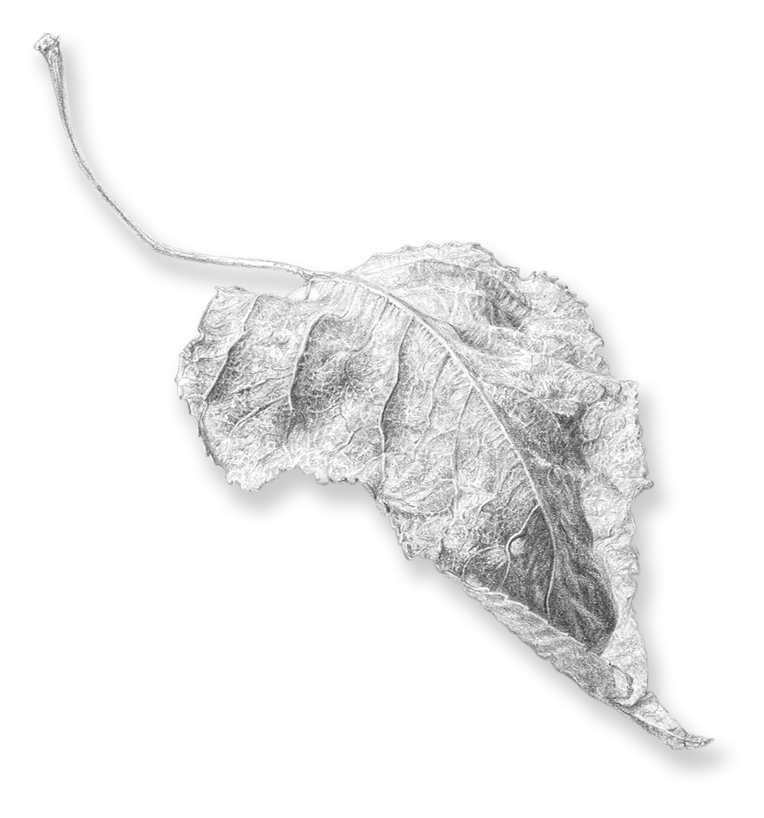
\includegraphics[height=1.5in,keepaspectratio,angle=25]{birch_by_Scott_illustration_Neil_CMYK.png}}}
%}{}
%
%\ifthenelse{\equal{\volumeTitle}{\textTitleVolOne}}{
%\newpage\mbox{}\thispagestyle{empty}
%}{}
%
%\ifthenelse{\equal{\volumeTitle}{\textTitleVolTwo}}{
%\newpage\mbox{}\thispagestyle{empty}
%}{}

% TODO
%
% Adding the glossary words which were not referenced in the text, but other
% glossary entries link to them as "see..." or "see also..."

\glsaddnonum{bodhi-pakkhiya-dhamma}
\glsaddnonum{tilakkhana}
\glsaddnonum{ariya-sacca}
\glsaddnonum{tisarana}
\glsaddnonum{mahathera}
\glsaddnonum{sabhava-dhamma}
\glsaddnonum{four-noble-truths}
\glsaddnonum{pativedha}
\glsaddnonum{adhitthana}
\glsaddnonum{sacca}
\glsaddnonum{anagarika}
\glsaddnonum{raga}
\glsaddnonum{brahma-vihara}
\glsaddnonum{brahmacariya}
\glsaddnonum{gotrabhu-nana}
\glsaddnonum{pabbajja}
\glsaddnonum{satipatthana}
\glsaddnonum{dhana}
\glsaddnonum{anupubbi-katha}
\glsaddnonum{sanna}
\glsaddnonum{vedana}
\glsaddnonum{brahmana}
\glsaddnonum{upasampada}
\glsaddnonum{parisa}
\glsaddnonum{sangha}
\glsaddnonum{moha}
\glsaddnonum{kayagata-sati}
\glsaddnonum{samyojana}
\glsaddnonum{ajahn}
\glsaddnonum{anusaya}
\glsaddnonum{upasika}
\glsaddnonum{upasaka}
\glsaddnonum{bhikkhuni}
\glsaddnonum{mula}
\glsaddnonum{saddha}
\glsaddnonum{indriya}

\chapterFootnote{\textit{Note}: These definitions of terms have been collected from a number of free distribution publications of the Forest Sa\.ngha. We have also included material from `\textit{A Glossary of Pali and Buddhist Terms}' edited by John T. Bullitt, available at \href{http://www.accesstoinsight.org/glossary.html}{www.accesstoinsight.org/glossary.html}. All definitions have been revised for relevance to this publication.}

\chapter{Glossary}

\printglossaries


%
\renewcommand\indexname{Index of Similes}
\printindex[similes]

\renewcommand\indexname{General Index}
\printindex[general]


%
\compactChapter{Sources of Talks}
\begingroup\setlength{\parindent}{0pt}\setlength{\parskip}{1.2em}


\newcommand*{\sourceTitle}[1]{{\chapterfont\normalsize\soChapter{\MakeUppercase{#1}}}}

\vspace*{-\baselineskip}
\sourceTitle{The Middle Way Within} \\
\textit{First published in:} A Taste of Freedom \\
\textit{Comment:} Given in the Northeastern dialect to an assembly of monks and laypeople in 1970.

\sourceTitle{The Peace Beyond} \\
\textit{First published in:} A Taste of Freedom \\
\textit{Comment:} A condensed version of a talk given to the Chief Privy Councillor of Thailand, Mr. Sanya Dharmasakti, at Wat Nong Pah Pong, 1978.

\sourceTitle{Convention and Liberation} \\
% \footnotetext[0]{\textit{Note}: A different translation of this talk has been published elsewhere under the title `Suppositions and Release' by Ajahn Thanissaro.}
\textit{First published in:} A Taste of Freedom \\
\textit{Comment:} An informal talk given in the Northeastern dialect, from an unidentified tape. \\
\textit{Note:} A different translation of this talk has been published elsewhere under the title `Suppositions and Release' by Ajahn Thanissaro.

\sourceTitle{No Abiding} \\
\textit{First published in:} A Taste of Freedom \\
\textit{Comment:} A talk given to the monks, novices and laypeople of Wat Pah Nanachat on a visit to Wat Nong Pah Pong during the rains of 1980.

\sourceTitle{Evening Sitting} \\
\textit{First published in:} The Path to Peace

\sourceTitle{About Being Careful} \\
\textit{First published in:} Everything is Teaching Us

\sourceTitle{It Can Be Done} \\
\textit{First published in:} Everything is Teaching Us

\sourceTitle{Understanding Dukkha} \\
\textit{First published in:} Everything is Teaching Us \\
\textit{Note:} This talk has been published elsewhere under the title `Giving up Good and Evil'.

\sourceTitle{The Dhamma Goes Westward} \\
\textit{First published in:} Everything is Teaching Us

\sourceTitle{Even One Word Is Enough} \\
\textit{First published in:} Everything is Teaching Us \\
\textit{Comment:} To the Western Sa\.ngha newly arrived in England, 1979.

\sourceTitle{Making the Heart Good} \\
\textit{First published in:} Living Dhamma \\
\textit{Comment:} Given on the occasion of a large group of laypeople coming to Wat Pah Pong to make offerings to support the monastery.

\sourceTitle{Why Are We Here?} \\
\textit{First published in:} Living Dhamma \\
\textit{Comment:} Given at Wat Tham Saeng Phet (The Monastery of the Diamond Light Cave) to a group of visiting laypeople, during the rains retreat of 1981, shortly before Ajahn Chah's health broke down.

\sourceTitle{Our Real Home} \\
\textit{First published in:} Living Dhamma \\
\textit{Comment:} A talk addressed to an aging lay disciple approaching her death.

\sourceTitle{The Four Noble Truths} \\
\textit{First published in:} Living Dhamma \\
\textit{Comment:} This talk was given at the Manjushri Institute in Cumbria, U.K., in 1977.

\clearpage

\sourceTitle{Living in the World} \\
\textit{First published in:} Living Dhamma \\
\textit{Comment:} An informal talk given after an invitation to receive almsfood at a lay person's house in Ubon, the district capital, close to Wat Pah Pong. \\
\textit{Note:} This talk has been published elsewhere under the title `Living in the World with Dhamma'.

\sourceTitle{Tuccho Pothila} \\
\textit{First published in:} Living Dhamma \\
\textit{Comment:} An informal talk given at Ajahn Chah's kuti, to a group of laypeople, one evening in 1978. \\
\textit{Note:} This talk has been published elsewhere under the title `Tuccho Pothila -- Venerable Empty-Scripture'.

\sourceTitle{Transcendence} \\
\textit{First published in:} Food for the Heart \\
\textit{Comment:} Given on a lunar observance night (uposatha), at Wat Pah Pong in 1975.

\sourceTitle{Timeless Teachings} \\
\textit{First published in:} Forest Sa\.ngha Newsletter, January 1997, Number 39

\sourceTitle{Fragments of a Teaching} \\
\textit{First published in:} Bodhinyana \\
\textit{Comment:} Given to the lay community at Wat Pah Pong in 1972.

\sourceTitle{A Gift of Dhamma} \\
\textit{First published in:} Bodhinyana \\
\textit{Comment:} A discourse delivered to the assembly of Western monks, novices and lay-disciples at Bung Wai Forest Monastery, Ubon, on the 10th of October, 1977. This discourse was offered to the parents of one of the monks on the occasion of their visit from France.

\clearpage

\sourceTitle{Living With the Cobra} \\
\textit{First published in:} Bodhinyana \\
\textit{Comment:} A brief talk given as final instruction to an elderly Englishwoman who spent two months under the guidance of Ajahn Chah at the end of 1978 and beginning of 1979.

\sourceTitle{Reading the Natural Mind} \\
\textit{First published in:} Bodhinyana \\
\textit{Comment:} An informal talk given to a group of newly ordained monks after the evening chanting, middle of the Rains Retreat, 1978.

\sourceTitle{Just Do It!} \\
\textit{First published in:} Bodhinyana \\
\textit{Comment:} A lively talk, in Lao dialect, given to the Assembly of newly-ordained Monks at Wat Pah Pong on the day of entering the Rains Retreat, July 1978. \\
\textit{Note:} A different translation of this talk has been published elsewhere under the title `Start Doing It!'.

\sourceTitle{Questions and Answers} \\
\textit{First published in:} Bodhinyana \\
\textit{Comment:} Notes taken over a period of a few days from a session of questions and answers with a group of Western monks, 1972. \\
\textit{Note:} This question and answer session was previously published under the same title in `Bodhinyana'.

\sourceTitle{Steady Practice} \\
\textit{First published in:} Food for the Heart \\
\textit{Comment:} Given at Wat Keuan to a group of university students who had taken temporary ordination, during the hot season of 1978. \\
\textit{Note:} This talk has been published elsewhere under the title `Right Practice -- Steady Practice'.

\clearpage

\sourceTitle{Detachment Within Activity} \\
\textit{First published in:} Food for the Heart \\
\textit{Comment:} Given at Wat Pah Pong during the rains retreat, 1977. \\
\textit{Note:} This talk has been published elsewhere under the title `Samm\={a} Sam\={a}dhi -- Detachment Within Activity'.

\sourceTitle{Training this Mind} \\
\textit{First published in:} A Taste of Freedom \\
\textit{Note:} A different translation of this talk has been published elsewhere under the title `About This Mind'.

\sourceTitle{Tranquillity and Insight} \\
\textit{First published in:} A Taste of Freedom \\
\textit{Comment:} An informal talk given in the Northeastern dialect, taken from an unidentified tape. \\
\textit{Note:} This talk has been published elsewhere under the title `On Meditation'.

\sourceTitle{The Path in Harmony} \\
\textit{First published in:} A Taste of Freedom \\
\textit{Comment:} A composite of two talks given in England in 1979 and 1977 respectively.

\sourceTitle{The Place of Coolness} \\
\textit{First published in:} A Taste of Freedom \\
\textit{Comment:} Given to the assembly of monks and novices at Wat Pah Nanachat, during the rains retreat, 1978. \\
\textit{Note:} This talk has been published elsewhere under the title `Right View -- the Place of Coolness'.

\clearpage

\sourceTitle{Monastery of Confusion} \\
\textit{First published in:} Everything is Teaching Us \\
\textit{Note:} This talk has been published elsewhere under the title `Free From Doubt'.

\sourceTitle{Knowing the World} \\
\textit{First published in:} Everything is Teaching Us \\
\textit{Note:} This talk has been published elsewhere under the title `Seeking the Source'.

\sourceTitle{Supports for Meditation} \\
\textit{First published in:} Living Dhamma \\
\textit{Comment:} Given at the Hampstead Vihara, London, 1977. \\
\textit{Note:} This talk has been published elsewhere under the title `Meditation'.

\sourceTitle{Still, Flowing Water} \\
\textit{First published in:} Living Dhamma \\
\textit{Comment:} Given at Wat Tham Saeng Phet, during the rains retreat of 1981.

\sourceTitle{Toward the Unconditioned} \\
\textit{First published in:} Living Dhamma \\
\textit{Comment:} Given on a lunar observance night (Uposatha) at Wat Pah Pong, 1976.

\sourceTitle{Clarity of Insight} \\
\textit{First published in:} Clarity of Insight \\
\textit{Comment:} A talk given to a group of lay meditators in Bangkok in April 1979.

\sourceTitle{Learning to Listen} \\
\textit{Comment:} Given in September 1978, at Wat Pah Pong.

\sourceTitle{Unshakeable Peace} \\
\textit{Comment:} Informally given to a visiting scholar monk who had come to pay respects to Venerable Ajahn Chah. \\
\textit{Note:} A different translation of this talk has been published elsewhere under the title `The Key to Liberation'.

\sourceTitle{Just This Much} \\
\textit{First published in:} A Taste of Freedom \\
\textit{Comment:} Taken from a talk given in England to a Western Dhamma student in 1977. \\
\textit{Note:} This talk has been previously published as `Epilogue' in `A Taste of Freedom'.

\sourceTitle{What Is Contemplation?} \\
\textit{First published in:} Seeing the Way Vol 1. \\
\textit{Comment:} This teaching is taken from a session of questions and answers that took place at Wat Gor Nork monastery during the Vassa of 1979, between Venerable Ajahn Chah and a group of English-speaking disciples. Some rearrangement of the sequence of conversation has been made for ease of understanding.

\sourceTitle{Dhamma Nature} \\
\textit{First published in:} Bodhinyana \\
\textit{Comment:} Delivered to the Western disciples at Bung Wai Forest Monastery during the rains retreat of 1977, just after one of the senior monks had disrobed and left the monastery.

\sourceTitle{Two Faces Of Reality} \\
\textit{First published in:} Bodhinyana \\
\textit{Comment:} A discourse delivered to the assembly of monks after the recitation of the \textit{p\=ati\-mokkha}, the monk's disciplinary code, at Wat Pah Pong during the rains retreat of 1976.

\sourceTitle{The Training of the Heart} \\
\textit{First published in:} Bodhinyana \\
\textit{Comment:} A talk given to a group of Western Monks from Wat Bovornives, Bangkok, March 1977. N.B. in this translation heart is used where mind was used in the other translations.

\sourceTitle{The Wave Ends} \\
\textit{First published in:} The Path to Peace \\
\textit{Comment:} Extracts from a conversation between Luang Por Chah and a lay Buddhist. \\
\textit{Note:} This talk has been previously published as `Questions and Answers' in `The Path to Peace'.

\sourceTitle{Dhamma Fighting} \\
\textit{First published in:} Food for the Heart \\
\textit{Comment:} Excerpt from a talk given to monks and novices at Wat Pah Pong.

\sourceTitle{Understanding Vinaya} \\
\textit{First published in:} Food for the Heart \\
\textit{Comment:} Given to the assembly of monks after the recitation of the \textit{p\=ati\-mokkha}, at Wat Pah Pong during the rains retreat of 1980.

\sourceTitle{Maintaining the Standard} \\
\textit{First published in:} Food for the Heart \\
\textit{Comment:} Given at Wat Pah Pong, after the completion of the Dhamma exams, 1978.

\sourceTitle{The Flood of Sensuality} \\
\textit{First published in:} Food for the Heart \\
\textit{Comment:} Given to the assembly of monks after the recitation of the \textit{p\=ati\-mokkha}, at Wat Pah Pong during the rains retreat, 1978.

\sourceTitle{In the Dead of Night \ldots} \\
\textit{First published in:} Food for the Heart \\
\textit{Comment:} Given on a lunar observance night (uposatha), at Wat Pah Pong, in the late 1960s.

\sourceTitle{The Fountain of Wisdom} \\
\textit{First published in:} Food for the Heart \\
\textit{Comment:} Given to the assembly of monks after the recitation of the \textit{p\=ati\-mokkha}, at Wat Pah Pong during the rains retreat, 1978. \\
\textit{Note:} This talk has been published elsewhere under the title `Sense Contact -- The Fountain of Wisdom'.

\sourceTitle{Not Sure} \\
\textit{First published in:} Food for the Heart \\
\textit{Comment:} An informal talk given at Ajahn Chah's kuti, to some monks and novices one evening in 1980. \\
\textit{Note:} This talk has been published elsewhere under the title `Not Sure! -- The Standard of the Noble Ones'.

\sourceTitle{Wholehearted Training} \\
\textit{First published in:} Everything is Teaching Us

\sourceTitle{Right Restraint} \\
\textit{First published in:} Everything is Teaching Us \\
\textit{Note:} The latter half of this talk has been published elsewhere under the title `Listening Beyond Words'.

\sourceTitle{Suffering on the Road} \\
\textit{First published in:} Living Dhamma \\
\textit{Comment:} A talk given to a group of monks preparing to leave the monastery and go off wandering after their fifth year under the guidance of Ajahn Chah.

\sourceTitle{Opening the Dhamma Eye} \\
\textit{First published in:} A Taste of Freedom \\
\textit{Comment:} Given at Wat Pah Pong to the assembly of monks and novices in October, 1968.

\clearpage

\sourceTitle{The Path to Peace} \\
\textit{First published in:} The Path to Peace

\sourceTitle{Toilets on the Path} \\
\textit{First published in:} Upalamani (Thai) \\
\textit{Comment:} This talk was originally given in the Lao language and translated into Central Thai for Luang Por Chah's biography, \pali{Upalamani}.

\sourceTitle{A Message from Thailand} \\
\textit{First published in:} Seeing the Way Vol 1. \\
\textit{Comment:} This message by Ajahn Chah was sent to his disciples in England whilst he was resident at a branch monastery called `The Cave of Diamond Light', just prior to the serious decline in his health during the rainy season retreat (vassa) of 1981.



\endgroup

%
\chapter{Further Resources}

\vspace*{-\baselineskip}
{\setlength{\parindent}{0pt}\setlength{\parskip}{1.2em}

\href{http://forestsangha.org/}{\large www.forestsangha.org}\\
A portal page to the Buddhist communities associated with Ven. Ajahn Chah. Current news announcements, information on the branch and associated monasteries, and other information can be found here.

% The Gallery feature was removed from forestsangha.org
%\href{http://forestsangha.org/gallery/}{\large www.forestsangha.org/gallery}\\
%This site offers a photo gallery of images of Ven. Ajahn Chah for personal, non-commercial use.

\href{http://forestsanghapublications.org/}{\large www.forestsanghapublications.org}\\
An extension of \href{http://forestsangha.org/}{www.forestsangha.org} providing links to free downloads of printed books and audio files. This site replaces \href{http://www.dhammathreads.org/}{www.dhammathreads.org} and \href{http://www.dhammatalks.org.uk/}{www.dhammatalks.org.uk}.

\href{http://amaravati.org/}{\large www.amaravati.org}\\
The website for Amaravati Buddhist Monastery in Hertfordshire, UK.

\href{http://www.abhayagiri.org/}{\large www.abhayagiri.org}\\
The website for Abhayagiri Buddhist Monastery in California, USA.

\href{http://watpahnanachat.org/}{\large www.watpahnanachat.org}\\
The website for Wat Pah Nanachat, the International Forest Monastery in Ubon, NE Thailand, a branch of Wat Nong Pah Pong.

\href{http://allisburning.org/}{\large www.allisburning.org}\\
An online photographic archive of places, people, objects and activities within the Therav\=ada Buddhist world.

\href{http://www.accesstoinsight.org/}{\large www.accesstoinsight.org}\\
A web resource for the study of Therav\=ada suttas and Dhamma translations.

}

%
\cleartoverso
\thispagestyle{empty}

% \markboth{Branch Monasteries}{\volumeTitle}%
\markboth{}{}%
\addcontentsline{toc}{chapter}{BRANCH MONASTERIES}%

{\centering

{\chapterTitleFont\chapterTitleSize\color{chaptertitle}\soChapter{\MakeUppercase{BRANCH MONASTERIES}}}

Western disciples of Ajahn Chah

The portal page for this community worldwide is:\\
\href{http://www.forestsangha.org}{www.forestsangha.org}
\vspace*{\baselineskip}

\setlength{\columnsep}{55pt}

\begin{minipage}{0.95\linewidth}
\begin{multicols}{2}
\setlength{\parindent}{0pt}
\setlength{\parskip}{1.2em}
\small

{\raggedright

\textbf{UNITED KINGDOM:} \\
Amaravati Buddhist Monastery\\
Great Gaddesden,\\
Hemel Hempstead,\\
Hertfordshire, HP1 3BZ\\
Tel. Office: +44 (0)144 284 2455\\
Fax. +44 (0)144 284 3721\\
Retreat Centre: \mbox{+44 (0)144 284 3239}\\
\href{http://www.amaravati.org}{www.amaravati.org}

\vfill

Aruna Ratanagiri\\
Harnham Buddhist Monastery\\
Harnham,\\
Belsay,\\
Northumberland, NE20 0HF\\
Tel. +44 (0)1661 881 612\\
Fax. +44 (0)1661 881 019\\
\href{http://www.ratanagiri.org.uk}{www.ratanagiri.org.uk}

\vfill

Cittaviveka\\
Chithurst Buddhist Monastery\\
Chithurst,\\
Petersfield,\\
Hampshire, GU31 5EU\\
Tel. +44 (0)1730 814 986\\
Fax. +44 (0)1730 817 334\\
\href{http://www.cittaviveka.org}{www.cittaviveka.org}

%\vfill
%
%Hartridge Buddhist Monastery\\
%Odle Cottage,\\
%Upottery,\\
%Honiton,\\
%Devon, EX14 9QE\\
%Tel. +44 (0)1404 89 1251\\
%Fax. +44 (0)1404 89 0023\\
%\href{http://www.hartridgemonastery.org}{www.hartridgemonastery.org}

}

\columnbreak

{\raggedright

\textbf{SWITZERLAND:} \\
Kloster Dhammapala\\
Am Waldrand,\\
CH-3718 Kandersteg\\
Tel. +41 (0)33 675 21 00\\
Fax. +41 (0)33 675 22 41\\
\href{http://www.dhammapala.ch}{www.dhammapala.ch}

\vfill

\textbf{THAILAND:} \\
Wat Pah Nanachat\\
Bahn Bung Wai,\\
Amper Warin,\\
Ubon 34310\\
\href{http://www.watpahnanachat.org}{www.watpahnanachat.org}

\vfill

\textbf{AUSTRALIA:} \\
Buddha Bodhivana Monastery\\
780 Woods Point Road,\\
East Warburton,\\
Vic 3799\\
Tel. +61 (0)3 5966 5999\\
Fax. +61 (0)3 5966 5998

\vfill

\textbf{NEW ZEALAND:} \\
Vimutti Buddhist Monastery\\
PO Box 7,\\
Bombay, 2343\\
(South Auckland)\\
\href{http://www.vimutti.org.nz}{www.vimutti.org.nz}

%\vfill
%
%Bodhinyanarama Monastery\\
%17 Rakau Grove,\\
%Stokes Valley,\\
%Lower Hutt 5019\\
%Tel. +64 (0)4 5637 193\\
%\href{http://www.bodhinyanarama.net.nz}{www.bodhinyanarama.net.nz}

}

\end{multicols}
\end{minipage}

\clearpage
\thispagestyle{empty}

{\chapterTitleSize\mbox{}}

\mbox{}

\mbox{} \\
\mbox{}
\vspace*{\baselineskip}

\begin{minipage}{0.95\linewidth}
\begin{multicols}{2}
\setlength{\parindent}{0pt}
\setlength{\parskip}{1.2em}
\small

{\raggedright

\textbf{UNITED STATES OF AMERICA:} \\
Abhayagiri Buddhist Monastery\\
16201 Tomki Road,\\
Redwood Valley,\\
CA 95470\\
Tel. +1 (707) 485 1630\\
\href{http://www.abhayagiri.org}{www.abhayagiri.org}

\textbf{ITALY:} \\
Santacittarama\\
Localita Brulla,\\
02030 Frasso Sabino (Rieti)\\
Tel. +39 07 6587 2186\\
Fax. +39 06 233 238 629\\
\href{http://www.santacittarama.org}{www.santacittarama.org}

}

\columnbreak

{\raggedright

\textbf{CANADA:} \\
Tisarana Buddhist Monastery\\
1356 Powers Road, RR \#3 Perth,\\
Ontario K7H 3C5\\
Phone: +1 613-264-8208\\
\href{http://www.tisarana.ca}{www.tisarana.ca}

%% Birken is not a branch monastery, it is an associated monastery
% Sitavana\\
% Birken Forest Monastery\\
% PO Box 5,\\
% Knutsford,\\
% VOE 2A0, BC\\
% \href{http://www.birken.ca}{www.birken.ca}

}

\end{multicols}
\end{minipage}

}



\cleardoublepage
\thispagestyle{empty}

{\centering\mbox{}\vspace*{\chaptopskip}\vspace*{3\baselineskip}

\begin{minipage}{0.8\linewidth}\smaller\centering\setlength{\parskip}{1em}\setlength{\parindent}{0em}

\textit{Sabbad\=ana\d{m} dhammad\=ana\d{m} jinati}\\
\vspace*{0.25\baselineskip}

The gift of Dhamma is greater than all other gifts.
\bigskip

\label{dont-sell}
This book is intended for free distribution. It should not be sold. It has been made available through the faith, effort and generosity of people who wish to share the understanding it contains with whomever is interested. This act of freely offering is itself part of what makes this a `Dhamma publication', a book based on spiritual values.

Please do not sell this book. If you no longer need it, please pass it on freely to another person. If you wish to help such publications to continue to be made available, you can make a contribution, however small or large, by either contacting one of our monasteries or by visiting\\ \href{http://forestsangha.org}{www.forestsangha.org}

\end{minipage}

}


\newpage
\thispagestyle{customplain}

{\ccdetailssize\setlength{\parindent}{0em}%
\raggedright

\label{cc-details}
{\centering

{\large\ccbyncnd}
\bigskip

This work is licenced under the\\ Creative Commons Attribution-NonCommercial-NoDerivs 2.0\\ UK: England \& Wales Licence. To view a copy of this licence, visit:\\
\href{http://creativecommons.org/licenses/by-nc-nd/2.0/uk/}{http://creativecommons.org/licenses/by-nc-nd/2.0/uk/}

}
\bigskip

Summary:
\bigskip

You are free:

\begin{packeditemize}
\item to copy, distribute, display and perform the work
\end{packeditemize}

Under the following conditions:
\begin{packeditemize}
\item Attribution: You must give the original author credit.
\item Non-Commercial: You may not use this work for commercial purposes.
\item No Derivative Works: You may not alter, transform, or build upon this work.
\end{packeditemize}

With the understanding that:
\begin{packeditemize}
\item Waiver: Any of the above conditions can be waived if you get permission from the copyright holder.
\item Public Domain: Where the work or any of its elements is in the public domain under applicable law, that status is in no way affected by the license.
\item Other Rights: In no way are any of the following rights affected by the license:
\begin{packeditemize}
\item Your fair dealing or fair use rights, or other applicable copyright exceptions and limitations;
\item The author's moral rights;
\item Rights other persons may have either in the work itself or in how the work is used, such as publicity or privacy rights.
\end{packeditemize}
\item Notice: For any reuse or distribution, you must make clear to others the licence terms of this work.
\end{packeditemize}

Harnham Buddhist Monastery Trust operating as Aruna Publications asserts its moral right to be identified as the author of this book.
\bigskip

Harnham Buddhist Monastery Trust requests that you attribute ownership of the work to Aruna Publications on copying, distribution, display or performance of the work.

}


%\newpage\mbox{}\thispagestyle{empty}
%\newpage\mbox{}\thispagestyle{empty}
\emptysheet

\end{document}
